\documentclass[twoside]{book}

% Packages required by doxygen
\usepackage{calc}
\usepackage{doxygen}
\usepackage{graphicx}
\usepackage[utf8]{inputenc}
\usepackage{makeidx}
\usepackage{multicol}
\usepackage{multirow}
\usepackage{textcomp}
\usepackage[table]{xcolor}

% Font selection
\usepackage[T1]{fontenc}
\usepackage{mathptmx}
\usepackage[scaled=.90]{helvet}
\usepackage{courier}
\usepackage{amssymb}
\usepackage{sectsty}
\renewcommand{\familydefault}{\sfdefault}
\allsectionsfont{%
  \fontseries{bc}\selectfont%
  \color{darkgray}%
}
\renewcommand{\DoxyLabelFont}{%
  \fontseries{bc}\selectfont%
  \color{darkgray}%
}

% Page & text layout
\usepackage{geometry}
\geometry{%
  a4paper,%
  top=2.5cm,%
  bottom=2.5cm,%
  left=2.5cm,%
  right=2.5cm%
}
\tolerance=750
\hfuzz=15pt
\hbadness=750
\setlength{\emergencystretch}{15pt}
\setlength{\parindent}{0cm}
\setlength{\parskip}{0.2cm}
\makeatletter
\renewcommand{\paragraph}{%
  \@startsection{paragraph}{4}{0ex}{-1.0ex}{1.0ex}{%
    \normalfont\normalsize\bfseries\SS@parafont%
  }%
}
\renewcommand{\subparagraph}{%
  \@startsection{subparagraph}{5}{0ex}{-1.0ex}{1.0ex}{%
    \normalfont\normalsize\bfseries\SS@subparafont%
  }%
}
\makeatother

% Headers & footers
\usepackage{fancyhdr}
\pagestyle{fancyplain}
\fancyhead[LE]{\fancyplain{}{\bfseries\thepage}}
\fancyhead[CE]{\fancyplain{}{}}
\fancyhead[RE]{\fancyplain{}{\bfseries\leftmark}}
\fancyhead[LO]{\fancyplain{}{\bfseries\rightmark}}
\fancyhead[CO]{\fancyplain{}{}}
\fancyhead[RO]{\fancyplain{}{\bfseries\thepage}}
\fancyfoot[LE]{\fancyplain{}{}}
\fancyfoot[CE]{\fancyplain{}{}}
\fancyfoot[RE]{\fancyplain{}{\bfseries\scriptsize Generated on Sun Aug 17 2014 16\-:02\-:24 for Ph2\-\_\-\-D\-A\-Q by Doxygen }}
\fancyfoot[LO]{\fancyplain{}{\bfseries\scriptsize Generated on Sun Aug 17 2014 16\-:02\-:24 for Ph2\-\_\-\-D\-A\-Q by Doxygen }}
\fancyfoot[CO]{\fancyplain{}{}}
\fancyfoot[RO]{\fancyplain{}{}}
\renewcommand{\footrulewidth}{0.4pt}
\renewcommand{\chaptermark}[1]{%
  \markboth{#1}{}%
}
\renewcommand{\sectionmark}[1]{%
  \markright{\thesection\ #1}%
}

% Indices & bibliography
\usepackage{natbib}
\usepackage[titles]{tocloft}
\setcounter{tocdepth}{3}
\setcounter{secnumdepth}{5}
\makeindex

% Hyperlinks (required, but should be loaded last)
\usepackage{ifpdf}
\ifpdf
  \usepackage[pdftex,pagebackref=true]{hyperref}
\else
  \usepackage[ps2pdf,pagebackref=true]{hyperref}
\fi
\hypersetup{%
  colorlinks=true,%
  linkcolor=blue,%
  citecolor=blue,%
  unicode%
}

% Custom commands
\newcommand{\clearemptydoublepage}{%
  \newpage{\pagestyle{empty}\cleardoublepage}%
}


%===== C O N T E N T S =====

\begin{document}

% Titlepage & ToC
\hypersetup{pageanchor=false}
\pagenumbering{roman}
\begin{titlepage}
\vspace*{7cm}
\begin{center}%
{\Large Ph2\-\_\-\-D\-A\-Q \\[1ex]\large 0.\-3 }\\
\vspace*{1cm}
{\large Generated by Doxygen 1.8.5}\\
\vspace*{0.5cm}
{\small Sun Aug 17 2014 16:02:24}\\
\end{center}
\end{titlepage}
\clearemptydoublepage
\tableofcontents
\clearemptydoublepage
\pagenumbering{arabic}
\hypersetup{pageanchor=true}

%--- Begin generated contents ---
\chapter{Git Repository for P\-H2\-\_\-\-D\-A\-Q Software}
\label{md__r_e_a_d_m_e}
\hypertarget{md__r_e_a_d_m_e}{}
Supposed to contain\-:


\begin{DoxyItemize}
\item A middleware A\-P\-I layer, implemented in C++, which will basically wrap to abstracted functions the firmware calls and handshakes currently hardcoded into D\-A\-Q systems software.
\item A C++ object-\/based library describing the system components (C\-B\-Cs, Hybrids, Boards) and their properties(values, status)
\item The standard X\-D\-A\-Q-\/based system, which could really benefit in its future versions of the previous two proposed A\-P\-Is.
\end{DoxyItemize}

\subsection*{M\-C\-P Test Interface }

Here are the step to make the program functional


\begin{DoxyEnumerate}
\item Recover the Git\-Hub repo with the latest tested version of the M\-C\-P.
\item Change in \hyperlink{_definition_8h}{H\-W\-Description/\-Definition.\-h} the path to the u\-Hal connection file.
\begin{DoxyItemize}
\item It's per default set to \-: \href{file:///afs/cern.ch/user/n/npierre/public/settings/connections.xml}{\tt file\-:///afs/cern.\-ch/user/n/npierre/public/settings/connections.\-xml}
\item You have to change it to \-: \href{file://$(BUILD)/settings/connections.xml}{\tt file\-://\$(\-B\-U\-I\-L\-D)/settings/connections.\-xml} (where  is the path to the root of the Git\-Hub repo you recovered)
\end{DoxyItemize}
\item Do a make in the root the repo
\item Launch testpgrm command if you want to test if everything is working good
\item Launch mcp to play with the Test Interface
\end{DoxyEnumerate}

\subsection*{What can you do with the software ? }

A Glib is created per default (maybe in the future you will be able to play with more than one Glib)

You can then add Modules to the Glib and Cbcs to the Modules you created. When creating a Cbc, you can choose the config file you will load to its register map. If you want to add your personal config file, please make sure to add it in \#define in the H\-W\-Description/\-Description.\-h and then to add an option in the M\-C\-P code.

After this creation round, you can do anything you want \-:
\begin{DoxyItemize}
\item Configure the Glib or the Cbcs
\item Manipulate the registers in the Glib
\item Manipulate the registers in the Cbcs
\item Do the manipulation to Start/\-Stop an acquisition, but not actually acquiring something relevant
\item Have a configuration recap of all the objects you created
\end{DoxyItemize}

Concerning the manipulation of the Cbcs, you have the opportunity to modify all the Cbcs of a same Module at once with the Broadcast feature of the Cbc.

When you write a register in the Glib or the Cbc, the writing is updated to the map contained in Glib/\-Cbc objects so that you're always fully aware of what is in the Glib/\-Cbc register.

For writing value in register, we invite you to put in the following format \-: 0x\-\_\-\-\_\-. You must thus type '0x\-F\-F' for exemple and not just 'F\-F' in the command line. That might change in the future..

At the end of the program, the register maps are saved into output\-\_\-\-X\-\_\-\-X.\-txt files you can find in the settings directory. For example, output\-\_\-1\-\_\-2.\-txt contains the register map of the Cbc 2 of the Module 1.

More features will be implemented later, so make sure to have the last release locally to benefit from them.

Warning ! \-: be careful with options choice in the program menus, some mistypes can leed to unexpected hazards \-:-\/(.

\subsection*{Future Improvements }

Implementation of generic Be\-Board and Be\-Board\-Interface Class which will help us dealing with multiple board type (Glib, F\-C7). Work on the Cbc class to make it recognize if the Cbc is from a Glib or a F\-C7. Implement the new Strasbourg firmware as soon as it comes out.

\subsection*{Support, Suggestions ? }

For any support/suggestions, mail Lorenzo Bidegain, Nicolas Pierre or Georg Auzinger. 
\chapter{Namespace Index}
\section{Namespace List}
Here is a list of all namespaces with brief descriptions\-:\begin{DoxyCompactList}
\item\contentsline{section}{\hyperlink{namespace_ph2___hw_description}{Ph2\-\_\-\-Hw\-Description} }{\pageref{namespace_ph2___hw_description}}{}
\item\contentsline{section}{\hyperlink{namespace_ph2___hw_interface}{Ph2\-\_\-\-Hw\-Interface} }{\pageref{namespace_ph2___hw_interface}}{}
\end{DoxyCompactList}

\chapter{Hierarchical Index}
\section{Class Hierarchy}
This inheritance list is sorted roughly, but not completely, alphabetically\-:\begin{DoxyCompactList}
\item \contentsline{section}{Ph2\-\_\-\-Hw\-Description\-:\-:Be\-Board}{\pageref{class_ph2___hw_description_1_1_be_board}}{}
\begin{DoxyCompactList}
\item \contentsline{section}{Ph2\-\_\-\-Hw\-Description\-:\-:Glib}{\pageref{class_ph2___hw_description_1_1_glib}}{}
\end{DoxyCompactList}
\item \contentsline{section}{Ph2\-\_\-\-Hw\-Description\-:\-:Cbc\-Comparer}{\pageref{struct_ph2___hw_description_1_1_cbc_comparer}}{}
\item \contentsline{section}{Ph2\-\_\-\-Hw\-Description\-:\-:Cbc\-Reg\-Item}{\pageref{struct_ph2___hw_description_1_1_cbc_reg_item}}{}
\item \contentsline{section}{Ph2\-\_\-\-Hw\-Interface\-:\-:Data}{\pageref{class_ph2___hw_interface_1_1_data}}{}
\item \contentsline{section}{Ph2\-\_\-\-Hw\-Interface\-:\-:Event}{\pageref{class_ph2___hw_interface_1_1_event}}{}
\item exception\begin{DoxyCompactList}
\item \contentsline{section}{Ph2\-\_\-\-Hw\-Interface\-:\-:Exception}{\pageref{class_ph2___hw_interface_1_1_exception}}{}
\end{DoxyCompactList}
\item \contentsline{section}{Ph2\-\_\-\-Hw\-Description\-:\-:Front\-End\-Description}{\pageref{class_ph2___hw_description_1_1_front_end_description}}{}
\begin{DoxyCompactList}
\item \contentsline{section}{Ph2\-\_\-\-Hw\-Description\-:\-:Cbc}{\pageref{class_ph2___hw_description_1_1_cbc}}{}
\item \contentsline{section}{Ph2\-\_\-\-Hw\-Description\-:\-:Module}{\pageref{class_ph2___hw_description_1_1_module}}{}
\end{DoxyCompactList}
\item \contentsline{section}{Ph2\-\_\-\-Hw\-Interface\-:\-:Reg\-Manager}{\pageref{class_ph2___hw_interface_1_1_reg_manager}}{}
\begin{DoxyCompactList}
\item \contentsline{section}{Ph2\-\_\-\-Hw\-Interface\-:\-:Be\-Board\-Interface}{\pageref{class_ph2___hw_interface_1_1_be_board_interface}}{}
\item \contentsline{section}{Ph2\-\_\-\-Hw\-Interface\-:\-:Cbc\-Interface}{\pageref{class_ph2___hw_interface_1_1_cbc_interface}}{}
\item \contentsline{section}{Ph2\-\_\-\-Hw\-Interface\-:\-:Glib\-Interface}{\pageref{class_ph2___hw_interface_1_1_glib_interface}}{}
\end{DoxyCompactList}
\end{DoxyCompactList}

\chapter{Data Structure Index}
\section{Class List}
Here are the classes, structs, unions and interfaces with brief descriptions\-:\begin{DoxyCompactList}
\item\contentsline{section}{\hyperlink{class_interface_1_1_h_w_interface}{Interface\-::\-H\-W\-Interface} }{\pageref{class_interface_1_1_h_w_interface}}{}
\end{DoxyCompactList}

\chapter{File Index}
\section{File List}
Here is a list of all files with brief descriptions\-:\begin{DoxyCompactList}
\item\contentsline{section}{H\-W\-Description/\hyperlink{_be_board_8cc}{Be\-Board.\-cc} }{\pageref{_be_board_8cc}}{}
\item\contentsline{section}{H\-W\-Description/\hyperlink{_be_board_8h}{Be\-Board.\-h} \\*Be\-Board Description class, configs of the Be\-Board }{\pageref{_be_board_8h}}{}
\item\contentsline{section}{H\-W\-Description/\hyperlink{_cbc_8cc}{Cbc.\-cc} }{\pageref{_cbc_8cc}}{}
\item\contentsline{section}{H\-W\-Description/\hyperlink{_cbc_8h}{Cbc.\-h} \\*Cbc Description class, config of the Cbcs }{\pageref{_cbc_8h}}{}
\item\contentsline{section}{H\-W\-Description/\hyperlink{_cbc_reg_item_8h}{Cbc\-Reg\-Item.\-h} \\*Cbc\-Reg\-Item description, contents of the structure Cbc\-Reg\-Item with is the value of the Cbc\-Reg\-Map }{\pageref{_cbc_reg_item_8h}}{}
\item\contentsline{section}{H\-W\-Description/\hyperlink{_definition_8h}{Definition.\-h} }{\pageref{_definition_8h}}{}
\item\contentsline{section}{H\-W\-Description/\hyperlink{_front_end_description_8cc}{Front\-End\-Description.\-cc} }{\pageref{_front_end_description_8cc}}{}
\item\contentsline{section}{H\-W\-Description/\hyperlink{_front_end_description_8h}{Front\-End\-Description.\-h} \\*Front\-End\-Description base class to describe all parameters common to all F\-E Components in the D\-A\-Q chain }{\pageref{_front_end_description_8h}}{}
\item\contentsline{section}{H\-W\-Description/\hyperlink{_module_8cc}{Module.\-cc} }{\pageref{_module_8cc}}{}
\item\contentsline{section}{H\-W\-Description/\hyperlink{_module_8h}{Module.\-h} \\*Module Description class }{\pageref{_module_8h}}{}
\item\contentsline{section}{H\-W\-Description/\hyperlink{_shelve_8cc}{Shelve.\-cc} }{\pageref{_shelve_8cc}}{}
\item\contentsline{section}{H\-W\-Description/\hyperlink{_shelve_8h}{Shelve.\-h} \\*Shelve Description class, handles a vector of Board }{\pageref{_shelve_8h}}{}
\item\contentsline{section}{H\-W\-Interface/\hyperlink{_be_board_f_w_interface_8cc}{Be\-Board\-F\-W\-Interface.\-cc} }{\pageref{_be_board_f_w_interface_8cc}}{}
\item\contentsline{section}{H\-W\-Interface/\hyperlink{_be_board_f_w_interface_8h}{Be\-Board\-F\-W\-Interface.\-h} \\*Be\-Board\-F\-W\-Interface base class of all type of boards }{\pageref{_be_board_f_w_interface_8h}}{}
\item\contentsline{section}{H\-W\-Interface/\hyperlink{_be_board_interface_8cc}{Be\-Board\-Interface.\-cc} }{\pageref{_be_board_interface_8cc}}{}
\item\contentsline{section}{H\-W\-Interface/\hyperlink{_be_board_interface_8h}{Be\-Board\-Interface.\-h} \\*User Interface to the Boards }{\pageref{_be_board_interface_8h}}{}
\item\contentsline{section}{H\-W\-Interface/\hyperlink{_cbc_interface_8cc}{Cbc\-Interface.\-cc} }{\pageref{_cbc_interface_8cc}}{}
\item\contentsline{section}{H\-W\-Interface/\hyperlink{_cbc_interface_8h}{Cbc\-Interface.\-h} \\*User Interface to the Cbcs }{\pageref{_cbc_interface_8h}}{}
\item\contentsline{section}{H\-W\-Interface/\hyperlink{_data_8cc}{Data.\-cc} }{\pageref{_data_8cc}}{}
\item\contentsline{section}{H\-W\-Interface/\hyperlink{_data_8h}{Data.\-h} }{\pageref{_data_8h}}{}
\item\contentsline{section}{H\-W\-Interface/\hyperlink{_event_8cc}{Event.\-cc} }{\pageref{_event_8cc}}{}
\item\contentsline{section}{H\-W\-Interface/\hyperlink{_event_8h}{Event.\-h} }{\pageref{_event_8h}}{}
\item\contentsline{section}{H\-W\-Interface/\hyperlink{_exception_8cc}{Exception.\-cc} }{\pageref{_exception_8cc}}{}
\item\contentsline{section}{H\-W\-Interface/\hyperlink{_exception_8h}{Exception.\-h} }{\pageref{_exception_8h}}{}
\item\contentsline{section}{H\-W\-Interface/\hyperlink{_glib_f_w_interface_8cc}{Glib\-F\-W\-Interface.\-cc} }{\pageref{_glib_f_w_interface_8cc}}{}
\item\contentsline{section}{H\-W\-Interface/\hyperlink{_glib_f_w_interface_8h}{Glib\-F\-W\-Interface.\-h} \\*Glib\-F\-W\-Interface init/config of the Glib and its Cbc's }{\pageref{_glib_f_w_interface_8h}}{}
\item\contentsline{section}{H\-W\-Interface/\hyperlink{_reg_manager_8cc}{Reg\-Manager.\-cc} }{\pageref{_reg_manager_8cc}}{}
\item\contentsline{section}{H\-W\-Interface/\hyperlink{_reg_manager_8h}{Reg\-Manager.\-h} \\*Reg\-Manager class, permit connection \& r/w registers }{\pageref{_reg_manager_8h}}{}
\item\contentsline{section}{H\-W\-Interface/\hyperlink{_utilities_8cc}{Utilities.\-cc} }{\pageref{_utilities_8cc}}{}
\item\contentsline{section}{H\-W\-Interface/\hyperlink{_utilities_8h}{Utilities.\-h} }{\pageref{_utilities_8h}}{}
\item\contentsline{section}{src/\hyperlink{mcp_8cc}{mcp.\-cc} }{\pageref{mcp_8cc}}{}
\item\contentsline{section}{src/\hyperlink{readdatatest2_c_b_c_8cc}{readdatatest2\-C\-B\-C.\-cc} }{\pageref{readdatatest2_c_b_c_8cc}}{}
\item\contentsline{section}{src/\hyperlink{readdatatest8_c_b_c_8cc}{readdatatest8\-C\-B\-C.\-cc} }{\pageref{readdatatest8_c_b_c_8cc}}{}
\item\contentsline{section}{src/\hyperlink{systemtest_8cc}{systemtest.\-cc} }{\pageref{systemtest_8cc}}{}
\item\contentsline{section}{src/\hyperlink{test_8cc}{test.\-cc} }{\pageref{test_8cc}}{}
\item\contentsline{section}{System/\hyperlink{pugiconfig_8hpp}{pugiconfig.\-hpp} }{\pageref{pugiconfig_8hpp}}{}
\item\contentsline{section}{System/\hyperlink{pugixml_8cpp}{pugixml.\-cpp} }{\pageref{pugixml_8cpp}}{}
\item\contentsline{section}{System/\hyperlink{pugixml_8hpp}{pugixml.\-hpp} }{\pageref{pugixml_8hpp}}{}
\item\contentsline{section}{System/\hyperlink{_system_controller_8cc}{System\-Controller.\-cc} }{\pageref{_system_controller_8cc}}{}
\item\contentsline{section}{System/\hyperlink{_system_controller_8h}{System\-Controller.\-h} \\*Controller of the System, overall wrapper of the framework }{\pageref{_system_controller_8h}}{}
\item\contentsline{section}{tools/\hyperlink{_calibration_8cc}{Calibration.\-cc} \\*\hyperlink{class_calibration}{Calibration} class, calibration of the hardware }{\pageref{_calibration_8cc}}{}
\item\contentsline{section}{tools/\hyperlink{_calibration_8h}{Calibration.\-h} \\*\hyperlink{class_calibration}{Calibration} class, calibration of the hardware }{\pageref{_calibration_8h}}{}
\item\contentsline{section}{tools/\hyperlink{_channel_8cc}{Channel.\-cc} }{\pageref{_channel_8cc}}{}
\item\contentsline{section}{tools/\hyperlink{_channel_8h}{Channel.\-h} }{\pageref{_channel_8h}}{}
\end{DoxyCompactList}

\chapter{Namespace Documentation}
\hypertarget{namespace_ph2___hw_description}{\section{Ph2\-\_\-\-Hw\-Description Namespace Reference}
\label{namespace_ph2___hw_description}\index{Ph2\-\_\-\-Hw\-Description@{Ph2\-\_\-\-Hw\-Description}}
}


Namespace regrouping all the hardware description.  


\subsection*{Data Structures}
\begin{DoxyCompactItemize}
\item 
class \hyperlink{class_ph2___hw_description_1_1_cbc}{Cbc}
\begin{DoxyCompactList}\small\item\em Read/\-Write \hyperlink{class_ph2___hw_description_1_1_cbc}{Cbc}'s registers on a file. \end{DoxyCompactList}\item 
struct \hyperlink{struct_ph2___hw_description_1_1_cbc_comparer}{Cbc\-Comparer}
\begin{DoxyCompactList}\small\item\em Compare two \hyperlink{class_ph2___hw_description_1_1_cbc}{Cbc} by their I\-D. \end{DoxyCompactList}\item 
struct \hyperlink{struct_ph2___hw_description_1_1_cbc_reg_item}{Cbc\-Reg\-Item}
\begin{DoxyCompactList}\small\item\em Struct for Cbc\-Register\-Item that is identified by (Name), Page, Address, Default\-Value, Value. \end{DoxyCompactList}\item 
class \hyperlink{class_ph2___hw_description_1_1_f_e_description}{F\-E\-Description}
\begin{DoxyCompactList}\small\item\em Describe all parameters common to all F\-E Components in the D\-A\-Q chain. \end{DoxyCompactList}\item 
class \hyperlink{class_ph2___hw_description_1_1_glib}{Glib}
\begin{DoxyCompactList}\small\item\em Read/\-Write \hyperlink{class_ph2___hw_description_1_1_glib}{Glib}'s registers on a file, contains a register map and contains a vector of \hyperlink{class_ph2___hw_description_1_1_module}{Module} which are connected to the \hyperlink{class_ph2___hw_description_1_1_glib}{Glib}. \end{DoxyCompactList}\item 
class \hyperlink{class_ph2___hw_description_1_1_module}{Module}
\begin{DoxyCompactList}\small\item\em contains a vector of \hyperlink{class_ph2___hw_description_1_1_cbc}{Cbc} which are connected to the \hyperlink{class_ph2___hw_description_1_1_module}{Module} \end{DoxyCompactList}\end{DoxyCompactItemize}
\subsection*{Typedefs}
\begin{DoxyCompactItemize}
\item 
typedef std\-::map$<$ std\-::string, \\*
\hyperlink{struct_ph2___hw_description_1_1_cbc_reg_item}{Cbc\-Reg\-Item} $>$ \hyperlink{namespace_ph2___hw_description_a9a23b373068f169aa67ca1d22c9a6001}{Cbc\-Reg\-Map}
\item 
typedef std\-::map$<$ std\-::string, \\*
uint8\-\_\-t $>$ \hyperlink{namespace_ph2___hw_description_afc0e75a92548c3406e89bf39ca4c9bfb}{Glib\-Reg\-Map}
\end{DoxyCompactItemize}
\subsection*{Enumerations}
\begin{DoxyCompactItemize}
\item 
enum \hyperlink{namespace_ph2___hw_description_a891c19542f306c932b747f42fe48fc2b}{nb\-\_\-\-F\-E} \{ \hyperlink{namespace_ph2___hw_description_a891c19542f306c932b747f42fe48fc2baa30d72f6d58dc25b003fbf8bf56b3ace}{S\-I\-N\-G\-L\-E\-\_\-\-F\-E}, 
\hyperlink{namespace_ph2___hw_description_a891c19542f306c932b747f42fe48fc2ba6e0b877d015d017f61b07618e057c452}{F\-E\-\_\-\-T\-R\-G}, 
\hyperlink{namespace_ph2___hw_description_a891c19542f306c932b747f42fe48fc2bae3b57cb16641bb367bfc57a00315a4ca}{D\-U\-A\-L\-\_\-\-F\-E}
 \}
\end{DoxyCompactItemize}


\subsection{Detailed Description}
Namespace regrouping all the hardware description. 

\subsection{Typedef Documentation}
\hypertarget{namespace_ph2___hw_description_a9a23b373068f169aa67ca1d22c9a6001}{\index{Ph2\-\_\-\-Hw\-Description@{Ph2\-\_\-\-Hw\-Description}!Cbc\-Reg\-Map@{Cbc\-Reg\-Map}}
\index{Cbc\-Reg\-Map@{Cbc\-Reg\-Map}!Ph2_HwDescription@{Ph2\-\_\-\-Hw\-Description}}
\subsubsection[{Cbc\-Reg\-Map}]{\setlength{\rightskip}{0pt plus 5cm}typedef std\-::map$<$ std\-::string, {\bf Cbc\-Reg\-Item} $>$ {\bf Ph2\-\_\-\-Hw\-Description\-::\-Cbc\-Reg\-Map}}}\label{namespace_ph2___hw_description_a9a23b373068f169aa67ca1d22c9a6001}
\hypertarget{namespace_ph2___hw_description_afc0e75a92548c3406e89bf39ca4c9bfb}{\index{Ph2\-\_\-\-Hw\-Description@{Ph2\-\_\-\-Hw\-Description}!Glib\-Reg\-Map@{Glib\-Reg\-Map}}
\index{Glib\-Reg\-Map@{Glib\-Reg\-Map}!Ph2_HwDescription@{Ph2\-\_\-\-Hw\-Description}}
\subsubsection[{Glib\-Reg\-Map}]{\setlength{\rightskip}{0pt plus 5cm}typedef std\-::map$<$ std\-::string, uint8\-\_\-t $>$ {\bf Ph2\-\_\-\-Hw\-Description\-::\-Glib\-Reg\-Map}}}\label{namespace_ph2___hw_description_afc0e75a92548c3406e89bf39ca4c9bfb}


\subsection{Enumeration Type Documentation}
\hypertarget{namespace_ph2___hw_description_a891c19542f306c932b747f42fe48fc2b}{\index{Ph2\-\_\-\-Hw\-Description@{Ph2\-\_\-\-Hw\-Description}!nb\-\_\-\-F\-E@{nb\-\_\-\-F\-E}}
\index{nb\-\_\-\-F\-E@{nb\-\_\-\-F\-E}!Ph2_HwDescription@{Ph2\-\_\-\-Hw\-Description}}
\subsubsection[{nb\-\_\-\-F\-E}]{\setlength{\rightskip}{0pt plus 5cm}enum {\bf Ph2\-\_\-\-Hw\-Description\-::nb\-\_\-\-F\-E}}}\label{namespace_ph2___hw_description_a891c19542f306c932b747f42fe48fc2b}
\begin{Desc}
\item[Enumerator]\par
\begin{description}
\index{S\-I\-N\-G\-L\-E\-\_\-\-F\-E@{S\-I\-N\-G\-L\-E\-\_\-\-F\-E}!Ph2\-\_\-\-Hw\-Description@{Ph2\-\_\-\-Hw\-Description}}\index{Ph2\-\_\-\-Hw\-Description@{Ph2\-\_\-\-Hw\-Description}!S\-I\-N\-G\-L\-E\-\_\-\-F\-E@{S\-I\-N\-G\-L\-E\-\_\-\-F\-E}}\item[{\em 
\hypertarget{namespace_ph2___hw_description_a891c19542f306c932b747f42fe48fc2baa30d72f6d58dc25b003fbf8bf56b3ace}{S\-I\-N\-G\-L\-E\-\_\-\-F\-E}\label{namespace_ph2___hw_description_a891c19542f306c932b747f42fe48fc2baa30d72f6d58dc25b003fbf8bf56b3ace}
}]\index{F\-E\-\_\-\-T\-R\-G@{F\-E\-\_\-\-T\-R\-G}!Ph2\-\_\-\-Hw\-Description@{Ph2\-\_\-\-Hw\-Description}}\index{Ph2\-\_\-\-Hw\-Description@{Ph2\-\_\-\-Hw\-Description}!F\-E\-\_\-\-T\-R\-G@{F\-E\-\_\-\-T\-R\-G}}\item[{\em 
\hypertarget{namespace_ph2___hw_description_a891c19542f306c932b747f42fe48fc2ba6e0b877d015d017f61b07618e057c452}{F\-E\-\_\-\-T\-R\-G}\label{namespace_ph2___hw_description_a891c19542f306c932b747f42fe48fc2ba6e0b877d015d017f61b07618e057c452}
}]\index{D\-U\-A\-L\-\_\-\-F\-E@{D\-U\-A\-L\-\_\-\-F\-E}!Ph2\-\_\-\-Hw\-Description@{Ph2\-\_\-\-Hw\-Description}}\index{Ph2\-\_\-\-Hw\-Description@{Ph2\-\_\-\-Hw\-Description}!D\-U\-A\-L\-\_\-\-F\-E@{D\-U\-A\-L\-\_\-\-F\-E}}\item[{\em 
\hypertarget{namespace_ph2___hw_description_a891c19542f306c932b747f42fe48fc2bae3b57cb16641bb367bfc57a00315a4ca}{D\-U\-A\-L\-\_\-\-F\-E}\label{namespace_ph2___hw_description_a891c19542f306c932b747f42fe48fc2bae3b57cb16641bb367bfc57a00315a4ca}
}]\end{description}
\end{Desc}

\hypertarget{namespace_ph2___hw_interface}{\section{Ph2\-\_\-\-Hw\-Interface Namespace Reference}
\label{namespace_ph2___hw_interface}\index{Ph2\-\_\-\-Hw\-Interface@{Ph2\-\_\-\-Hw\-Interface}}
}


Namespace regrouping all the interfaces to the hardware.  


\subsection*{Data Structures}
\begin{DoxyCompactItemize}
\item 
class \hyperlink{class_ph2___hw_interface_1_1_cbc_interface}{Cbc\-Interface}
\begin{DoxyCompactList}\small\item\em Permit r/w given registers in the Cbc you specify. \end{DoxyCompactList}\item 
class \hyperlink{class_ph2___hw_interface_1_1_exception}{Exception}
\item 
class \hyperlink{class_ph2___hw_interface_1_1_glib_interface}{Glib\-Interface}
\begin{DoxyCompactList}\small\item\em Permit r/w given registers in the Glib you specify. \end{DoxyCompactList}\item 
class \hyperlink{class_ph2___hw_interface_1_1_reg_manager}{Reg\-Manager}
\begin{DoxyCompactList}\small\item\em Permit connection to given boards and r/w given registers. \end{DoxyCompactList}\end{DoxyCompactItemize}
\subsection*{Functions}
\begin{DoxyCompactItemize}
\item 
long \hyperlink{namespace_ph2___hw_interface_a033a07cbe28368de19d534ef7cd3325d}{get\-Time\-Took} (struct timeval \&p\-Start, bool p\-Mili)
\item 
void \hyperlink{namespace_ph2___hw_interface_a2fe2ee1ddb69c79c23bf9b0b2fa58f67}{myflush} (std\-::istream \&in)
\item 
void \hyperlink{namespace_ph2___hw_interface_a20399ed909de2641f1e7e086a4ec3667}{mypause} ()
\end{DoxyCompactItemize}


\subsection{Detailed Description}
Namespace regrouping all the interfaces to the hardware. 

\subsection{Function Documentation}
\hypertarget{namespace_ph2___hw_interface_a033a07cbe28368de19d534ef7cd3325d}{\index{Ph2\-\_\-\-Hw\-Interface@{Ph2\-\_\-\-Hw\-Interface}!get\-Time\-Took@{get\-Time\-Took}}
\index{get\-Time\-Took@{get\-Time\-Took}!Ph2_HwInterface@{Ph2\-\_\-\-Hw\-Interface}}
\subsubsection[{get\-Time\-Took}]{\setlength{\rightskip}{0pt plus 5cm}long Ph2\-\_\-\-Hw\-Interface\-::get\-Time\-Took (
\begin{DoxyParamCaption}
\item[{struct timeval \&}]{p\-Start, }
\item[{bool}]{p\-Mili}
\end{DoxyParamCaption}
)}}\label{namespace_ph2___hw_interface_a033a07cbe28368de19d534ef7cd3325d}
\hypertarget{namespace_ph2___hw_interface_a2fe2ee1ddb69c79c23bf9b0b2fa58f67}{\index{Ph2\-\_\-\-Hw\-Interface@{Ph2\-\_\-\-Hw\-Interface}!myflush@{myflush}}
\index{myflush@{myflush}!Ph2_HwInterface@{Ph2\-\_\-\-Hw\-Interface}}
\subsubsection[{myflush}]{\setlength{\rightskip}{0pt plus 5cm}void Ph2\-\_\-\-Hw\-Interface\-::myflush (
\begin{DoxyParamCaption}
\item[{std\-::istream \&}]{in}
\end{DoxyParamCaption}
)}}\label{namespace_ph2___hw_interface_a2fe2ee1ddb69c79c23bf9b0b2fa58f67}
\hypertarget{namespace_ph2___hw_interface_a20399ed909de2641f1e7e086a4ec3667}{\index{Ph2\-\_\-\-Hw\-Interface@{Ph2\-\_\-\-Hw\-Interface}!mypause@{mypause}}
\index{mypause@{mypause}!Ph2_HwInterface@{Ph2\-\_\-\-Hw\-Interface}}
\subsubsection[{mypause}]{\setlength{\rightskip}{0pt plus 5cm}void Ph2\-\_\-\-Hw\-Interface\-::mypause (
\begin{DoxyParamCaption}
{}
\end{DoxyParamCaption}
)}}\label{namespace_ph2___hw_interface_a20399ed909de2641f1e7e086a4ec3667}

\hypertarget{namespace_ph2___system}{\section{Ph2\-\_\-\-System Namespace Reference}
\label{namespace_ph2___system}\index{Ph2\-\_\-\-System@{Ph2\-\_\-\-System}}
}


Namespace regrouping the framework wrapper.  


\subsection*{Data Structures}
\begin{DoxyCompactItemize}
\item 
class \hyperlink{class_ph2___system_1_1_system_controller}{System\-Controller}
\begin{DoxyCompactList}\small\item\em Create, initialise, configure a predefined H\-W structure. \end{DoxyCompactList}\end{DoxyCompactItemize}
\subsection*{Typedefs}
\begin{DoxyCompactItemize}
\item 
typedef std\-::vector$<$ \hyperlink{class_ph2___hw_description_1_1_shelve}{Shelve} $\ast$ $>$ \hyperlink{namespace_ph2___system_a1c21eed494ab8a888694adf3de379dcf}{Shelve\-Vec}
\item 
typedef std\-::map$<$ std\-::string, \\*
uint8\-\_\-t $>$ \hyperlink{namespace_ph2___system_a0ea674c0ee02ac6834ac9a1335111980}{Settings\-Map}
\end{DoxyCompactItemize}


\subsection{Detailed Description}
Namespace regrouping the framework wrapper. 

\subsection{Typedef Documentation}
\hypertarget{namespace_ph2___system_a0ea674c0ee02ac6834ac9a1335111980}{\index{Ph2\-\_\-\-System@{Ph2\-\_\-\-System}!Settings\-Map@{Settings\-Map}}
\index{Settings\-Map@{Settings\-Map}!Ph2_System@{Ph2\-\_\-\-System}}
\subsubsection[{Settings\-Map}]{\setlength{\rightskip}{0pt plus 5cm}typedef std\-::map$<$std\-::string,uint8\-\_\-t$>$ {\bf Ph2\-\_\-\-System\-::\-Settings\-Map}}}\label{namespace_ph2___system_a0ea674c0ee02ac6834ac9a1335111980}
Maps the settings \hypertarget{namespace_ph2___system_a1c21eed494ab8a888694adf3de379dcf}{\index{Ph2\-\_\-\-System@{Ph2\-\_\-\-System}!Shelve\-Vec@{Shelve\-Vec}}
\index{Shelve\-Vec@{Shelve\-Vec}!Ph2_System@{Ph2\-\_\-\-System}}
\subsubsection[{Shelve\-Vec}]{\setlength{\rightskip}{0pt plus 5cm}typedef std\-::vector$<${\bf Shelve}$\ast$$>$ {\bf Ph2\-\_\-\-System\-::\-Shelve\-Vec}}}\label{namespace_ph2___system_a1c21eed494ab8a888694adf3de379dcf}
Vector of Shelve pointers 
\hypertarget{namespacepugi}{\section{pugi Namespace Reference}
\label{namespacepugi}\index{pugi@{pugi}}
}
\subsection*{Data Structures}
\begin{DoxyCompactItemize}
\item 
struct \hyperlink{structpugi_1_1xml__attribute__struct}{xml\-\_\-attribute\-\_\-struct}
\begin{DoxyCompactList}\small\item\em A 'name=value' X\-M\-L attribute structure. \end{DoxyCompactList}\item 
struct \hyperlink{structpugi_1_1xml__node__struct}{xml\-\_\-node\-\_\-struct}
\begin{DoxyCompactList}\small\item\em An X\-M\-L document tree node. \end{DoxyCompactList}\end{DoxyCompactItemize}
\subsection*{Functions}
\begin{DoxyCompactItemize}
\item 
static \hyperlink{pugixml_8cpp_a82c335af3ca48cdb209c506bf8dd6ad2}{P\-U\-G\-I\-\_\-\-\_\-\-F\-N} void \hyperlink{namespacepugi_a8effe3a6fc7cc9c1cf2550739dbdc438}{unspecified\-\_\-bool\-\_\-xml\-\_\-attribute} (xml\-\_\-attribute $\ast$$\ast$$\ast$)
\item 
static \hyperlink{pugixml_8cpp_a82c335af3ca48cdb209c506bf8dd6ad2}{P\-U\-G\-I\-\_\-\-\_\-\-F\-N} void \hyperlink{namespacepugi_a487b2e720a3808d6fd5730d7c97bcdac}{unspecified\-\_\-bool\-\_\-xml\-\_\-node} (xml\-\_\-node $\ast$$\ast$$\ast$)
\item 
static \hyperlink{pugixml_8cpp_a82c335af3ca48cdb209c506bf8dd6ad2}{P\-U\-G\-I\-\_\-\-\_\-\-F\-N} void \hyperlink{namespacepugi_acfae514de3abac05ed155e531a401c15}{unspecified\-\_\-bool\-\_\-xml\-\_\-text} (xml\-\_\-text $\ast$$\ast$$\ast$)
\item 
\hyperlink{pugixml_8cpp_a82c335af3ca48cdb209c506bf8dd6ad2}{P\-U\-G\-I\-\_\-\-\_\-\-F\-N} std\-::string \\*
P\-U\-G\-I\-X\-M\-L\-\_\-\-F\-U\-N\-C\-T\-I\-O\-N \hyperlink{namespacepugi_a390bb44f7ba92b1a8a4f9157799d2ca8}{as\-\_\-utf8} (const wchar\-\_\-t $\ast$str)
\item 
\hyperlink{pugixml_8cpp_a82c335af3ca48cdb209c506bf8dd6ad2}{P\-U\-G\-I\-\_\-\-\_\-\-F\-N} std\-::string \\*
P\-U\-G\-I\-X\-M\-L\-\_\-\-F\-U\-N\-C\-T\-I\-O\-N \hyperlink{namespacepugi_ab4be9ab3dc86b13599b9f2fd2f778dfb}{as\-\_\-utf8} (const std\-::basic\-\_\-string$<$ wchar\-\_\-t $>$ \&str)
\item 
\hyperlink{pugixml_8cpp_a82c335af3ca48cdb209c506bf8dd6ad2}{P\-U\-G\-I\-\_\-\-\_\-\-F\-N} std\-::basic\-\_\-string\\*
$<$ wchar\-\_\-t $>$ P\-U\-G\-I\-X\-M\-L\-\_\-\-F\-U\-N\-C\-T\-I\-O\-N \hyperlink{namespacepugi_ac2a9782a1c3c725703c6e4533e735d9b}{as\-\_\-wide} (const char $\ast$str)
\item 
\hyperlink{pugixml_8cpp_a82c335af3ca48cdb209c506bf8dd6ad2}{P\-U\-G\-I\-\_\-\-\_\-\-F\-N} std\-::basic\-\_\-string\\*
$<$ wchar\-\_\-t $>$ P\-U\-G\-I\-X\-M\-L\-\_\-\-F\-U\-N\-C\-T\-I\-O\-N \hyperlink{namespacepugi_af33046c0db1ff7b3f63327d32fc6dca7}{as\-\_\-wide} (const std\-::string \&str)
\item 
\hyperlink{pugixml_8cpp_a82c335af3ca48cdb209c506bf8dd6ad2}{P\-U\-G\-I\-\_\-\-\_\-\-F\-N} void P\-U\-G\-I\-X\-M\-L\-\_\-\-F\-U\-N\-C\-T\-I\-O\-N \hyperlink{namespacepugi_a993c6b7947c1dec98936510d9e5fe778}{set\-\_\-memory\-\_\-management\-\_\-functions} (allocation\-\_\-function allocate, deallocation\-\_\-function deallocate)
\item 
\hyperlink{pugixml_8cpp_a82c335af3ca48cdb209c506bf8dd6ad2}{P\-U\-G\-I\-\_\-\-\_\-\-F\-N} allocation\-\_\-function \\*
P\-U\-G\-I\-X\-M\-L\-\_\-\-F\-U\-N\-C\-T\-I\-O\-N \hyperlink{namespacepugi_ab36e5aed4e5c952687b42d69daf981eb}{get\-\_\-memory\-\_\-allocation\-\_\-function} ()
\item 
\hyperlink{pugixml_8cpp_a82c335af3ca48cdb209c506bf8dd6ad2}{P\-U\-G\-I\-\_\-\-\_\-\-F\-N} deallocation\-\_\-function \\*
P\-U\-G\-I\-X\-M\-L\-\_\-\-F\-U\-N\-C\-T\-I\-O\-N \hyperlink{namespacepugi_a9fcabe4b52fbef0f133fab9ff97652ca}{get\-\_\-memory\-\_\-deallocation\-\_\-function} ()
\item 
static \hyperlink{pugixml_8cpp_a82c335af3ca48cdb209c506bf8dd6ad2}{P\-U\-G\-I\-\_\-\-\_\-\-F\-N} void \hyperlink{namespacepugi_abca519e72b848d2ebadf5250727da6c5}{unspecified\-\_\-bool\-\_\-xpath\-\_\-node} (xpath\-\_\-node $\ast$$\ast$$\ast$)
\item 
static \hyperlink{pugixml_8cpp_a82c335af3ca48cdb209c506bf8dd6ad2}{P\-U\-G\-I\-\_\-\-\_\-\-F\-N} void \hyperlink{namespacepugi_a41b925609dde7657664cf68c6506838b}{unspecified\-\_\-bool\-\_\-xpath\-\_\-query} (xpath\-\_\-query $\ast$$\ast$$\ast$)
\end{DoxyCompactItemize}


\subsection{Function Documentation}
\hypertarget{namespacepugi_a390bb44f7ba92b1a8a4f9157799d2ca8}{\index{pugi@{pugi}!as\-\_\-utf8@{as\-\_\-utf8}}
\index{as\-\_\-utf8@{as\-\_\-utf8}!pugi@{pugi}}
\subsubsection[{as\-\_\-utf8}]{\setlength{\rightskip}{0pt plus 5cm}{\bf P\-U\-G\-I\-\_\-\-\_\-\-F\-N} std\-::string P\-U\-G\-I\-X\-M\-L\-\_\-\-F\-U\-N\-C\-T\-I\-O\-N pugi\-::as\-\_\-utf8 (
\begin{DoxyParamCaption}
\item[{const wchar\-\_\-t $\ast$}]{str}
\end{DoxyParamCaption}
)}}\label{namespacepugi_a390bb44f7ba92b1a8a4f9157799d2ca8}
\hypertarget{namespacepugi_ab4be9ab3dc86b13599b9f2fd2f778dfb}{\index{pugi@{pugi}!as\-\_\-utf8@{as\-\_\-utf8}}
\index{as\-\_\-utf8@{as\-\_\-utf8}!pugi@{pugi}}
\subsubsection[{as\-\_\-utf8}]{\setlength{\rightskip}{0pt plus 5cm}{\bf P\-U\-G\-I\-\_\-\-\_\-\-F\-N} std\-::string P\-U\-G\-I\-X\-M\-L\-\_\-\-F\-U\-N\-C\-T\-I\-O\-N pugi\-::as\-\_\-utf8 (
\begin{DoxyParamCaption}
\item[{const std\-::basic\-\_\-string$<$ wchar\-\_\-t $>$ \&}]{str}
\end{DoxyParamCaption}
)}}\label{namespacepugi_ab4be9ab3dc86b13599b9f2fd2f778dfb}
\hypertarget{namespacepugi_ac2a9782a1c3c725703c6e4533e735d9b}{\index{pugi@{pugi}!as\-\_\-wide@{as\-\_\-wide}}
\index{as\-\_\-wide@{as\-\_\-wide}!pugi@{pugi}}
\subsubsection[{as\-\_\-wide}]{\setlength{\rightskip}{0pt plus 5cm}{\bf P\-U\-G\-I\-\_\-\-\_\-\-F\-N} std\-::basic\-\_\-string$<$wchar\-\_\-t$>$ P\-U\-G\-I\-X\-M\-L\-\_\-\-F\-U\-N\-C\-T\-I\-O\-N pugi\-::as\-\_\-wide (
\begin{DoxyParamCaption}
\item[{const char $\ast$}]{str}
\end{DoxyParamCaption}
)}}\label{namespacepugi_ac2a9782a1c3c725703c6e4533e735d9b}
\hypertarget{namespacepugi_af33046c0db1ff7b3f63327d32fc6dca7}{\index{pugi@{pugi}!as\-\_\-wide@{as\-\_\-wide}}
\index{as\-\_\-wide@{as\-\_\-wide}!pugi@{pugi}}
\subsubsection[{as\-\_\-wide}]{\setlength{\rightskip}{0pt plus 5cm}{\bf P\-U\-G\-I\-\_\-\-\_\-\-F\-N} std\-::basic\-\_\-string$<$wchar\-\_\-t$>$ P\-U\-G\-I\-X\-M\-L\-\_\-\-F\-U\-N\-C\-T\-I\-O\-N pugi\-::as\-\_\-wide (
\begin{DoxyParamCaption}
\item[{const std\-::string \&}]{str}
\end{DoxyParamCaption}
)}}\label{namespacepugi_af33046c0db1ff7b3f63327d32fc6dca7}
\hypertarget{namespacepugi_ab36e5aed4e5c952687b42d69daf981eb}{\index{pugi@{pugi}!get\-\_\-memory\-\_\-allocation\-\_\-function@{get\-\_\-memory\-\_\-allocation\-\_\-function}}
\index{get\-\_\-memory\-\_\-allocation\-\_\-function@{get\-\_\-memory\-\_\-allocation\-\_\-function}!pugi@{pugi}}
\subsubsection[{get\-\_\-memory\-\_\-allocation\-\_\-function}]{\setlength{\rightskip}{0pt plus 5cm}{\bf P\-U\-G\-I\-\_\-\-\_\-\-F\-N} allocation\-\_\-function P\-U\-G\-I\-X\-M\-L\-\_\-\-F\-U\-N\-C\-T\-I\-O\-N pugi\-::get\-\_\-memory\-\_\-allocation\-\_\-function (
\begin{DoxyParamCaption}
{}
\end{DoxyParamCaption}
)}}\label{namespacepugi_ab36e5aed4e5c952687b42d69daf981eb}
\hypertarget{namespacepugi_a9fcabe4b52fbef0f133fab9ff97652ca}{\index{pugi@{pugi}!get\-\_\-memory\-\_\-deallocation\-\_\-function@{get\-\_\-memory\-\_\-deallocation\-\_\-function}}
\index{get\-\_\-memory\-\_\-deallocation\-\_\-function@{get\-\_\-memory\-\_\-deallocation\-\_\-function}!pugi@{pugi}}
\subsubsection[{get\-\_\-memory\-\_\-deallocation\-\_\-function}]{\setlength{\rightskip}{0pt plus 5cm}{\bf P\-U\-G\-I\-\_\-\-\_\-\-F\-N} deallocation\-\_\-function P\-U\-G\-I\-X\-M\-L\-\_\-\-F\-U\-N\-C\-T\-I\-O\-N pugi\-::get\-\_\-memory\-\_\-deallocation\-\_\-function (
\begin{DoxyParamCaption}
{}
\end{DoxyParamCaption}
)}}\label{namespacepugi_a9fcabe4b52fbef0f133fab9ff97652ca}
\hypertarget{namespacepugi_a993c6b7947c1dec98936510d9e5fe778}{\index{pugi@{pugi}!set\-\_\-memory\-\_\-management\-\_\-functions@{set\-\_\-memory\-\_\-management\-\_\-functions}}
\index{set\-\_\-memory\-\_\-management\-\_\-functions@{set\-\_\-memory\-\_\-management\-\_\-functions}!pugi@{pugi}}
\subsubsection[{set\-\_\-memory\-\_\-management\-\_\-functions}]{\setlength{\rightskip}{0pt plus 5cm}{\bf P\-U\-G\-I\-\_\-\-\_\-\-F\-N} void P\-U\-G\-I\-X\-M\-L\-\_\-\-F\-U\-N\-C\-T\-I\-O\-N pugi\-::set\-\_\-memory\-\_\-management\-\_\-functions (
\begin{DoxyParamCaption}
\item[{allocation\-\_\-function}]{allocate, }
\item[{deallocation\-\_\-function}]{deallocate}
\end{DoxyParamCaption}
)}}\label{namespacepugi_a993c6b7947c1dec98936510d9e5fe778}
\hypertarget{namespacepugi_a8effe3a6fc7cc9c1cf2550739dbdc438}{\index{pugi@{pugi}!unspecified\-\_\-bool\-\_\-xml\-\_\-attribute@{unspecified\-\_\-bool\-\_\-xml\-\_\-attribute}}
\index{unspecified\-\_\-bool\-\_\-xml\-\_\-attribute@{unspecified\-\_\-bool\-\_\-xml\-\_\-attribute}!pugi@{pugi}}
\subsubsection[{unspecified\-\_\-bool\-\_\-xml\-\_\-attribute}]{\setlength{\rightskip}{0pt plus 5cm}static {\bf P\-U\-G\-I\-\_\-\-\_\-\-F\-N} void pugi\-::unspecified\-\_\-bool\-\_\-xml\-\_\-attribute (
\begin{DoxyParamCaption}
\item[{xml\-\_\-attribute $\ast$$\ast$$\ast$}]{}
\end{DoxyParamCaption}
)\hspace{0.3cm}{\ttfamily [static]}}}\label{namespacepugi_a8effe3a6fc7cc9c1cf2550739dbdc438}
\hypertarget{namespacepugi_a487b2e720a3808d6fd5730d7c97bcdac}{\index{pugi@{pugi}!unspecified\-\_\-bool\-\_\-xml\-\_\-node@{unspecified\-\_\-bool\-\_\-xml\-\_\-node}}
\index{unspecified\-\_\-bool\-\_\-xml\-\_\-node@{unspecified\-\_\-bool\-\_\-xml\-\_\-node}!pugi@{pugi}}
\subsubsection[{unspecified\-\_\-bool\-\_\-xml\-\_\-node}]{\setlength{\rightskip}{0pt plus 5cm}static {\bf P\-U\-G\-I\-\_\-\-\_\-\-F\-N} void pugi\-::unspecified\-\_\-bool\-\_\-xml\-\_\-node (
\begin{DoxyParamCaption}
\item[{xml\-\_\-node $\ast$$\ast$$\ast$}]{}
\end{DoxyParamCaption}
)\hspace{0.3cm}{\ttfamily [static]}}}\label{namespacepugi_a487b2e720a3808d6fd5730d7c97bcdac}
\hypertarget{namespacepugi_acfae514de3abac05ed155e531a401c15}{\index{pugi@{pugi}!unspecified\-\_\-bool\-\_\-xml\-\_\-text@{unspecified\-\_\-bool\-\_\-xml\-\_\-text}}
\index{unspecified\-\_\-bool\-\_\-xml\-\_\-text@{unspecified\-\_\-bool\-\_\-xml\-\_\-text}!pugi@{pugi}}
\subsubsection[{unspecified\-\_\-bool\-\_\-xml\-\_\-text}]{\setlength{\rightskip}{0pt plus 5cm}static {\bf P\-U\-G\-I\-\_\-\-\_\-\-F\-N} void pugi\-::unspecified\-\_\-bool\-\_\-xml\-\_\-text (
\begin{DoxyParamCaption}
\item[{xml\-\_\-text $\ast$$\ast$$\ast$}]{}
\end{DoxyParamCaption}
)\hspace{0.3cm}{\ttfamily [static]}}}\label{namespacepugi_acfae514de3abac05ed155e531a401c15}
\hypertarget{namespacepugi_abca519e72b848d2ebadf5250727da6c5}{\index{pugi@{pugi}!unspecified\-\_\-bool\-\_\-xpath\-\_\-node@{unspecified\-\_\-bool\-\_\-xpath\-\_\-node}}
\index{unspecified\-\_\-bool\-\_\-xpath\-\_\-node@{unspecified\-\_\-bool\-\_\-xpath\-\_\-node}!pugi@{pugi}}
\subsubsection[{unspecified\-\_\-bool\-\_\-xpath\-\_\-node}]{\setlength{\rightskip}{0pt plus 5cm}static {\bf P\-U\-G\-I\-\_\-\-\_\-\-F\-N} void pugi\-::unspecified\-\_\-bool\-\_\-xpath\-\_\-node (
\begin{DoxyParamCaption}
\item[{xpath\-\_\-node $\ast$$\ast$$\ast$}]{}
\end{DoxyParamCaption}
)\hspace{0.3cm}{\ttfamily [static]}}}\label{namespacepugi_abca519e72b848d2ebadf5250727da6c5}
\hypertarget{namespacepugi_a41b925609dde7657664cf68c6506838b}{\index{pugi@{pugi}!unspecified\-\_\-bool\-\_\-xpath\-\_\-query@{unspecified\-\_\-bool\-\_\-xpath\-\_\-query}}
\index{unspecified\-\_\-bool\-\_\-xpath\-\_\-query@{unspecified\-\_\-bool\-\_\-xpath\-\_\-query}!pugi@{pugi}}
\subsubsection[{unspecified\-\_\-bool\-\_\-xpath\-\_\-query}]{\setlength{\rightskip}{0pt plus 5cm}static {\bf P\-U\-G\-I\-\_\-\-\_\-\-F\-N} void pugi\-::unspecified\-\_\-bool\-\_\-xpath\-\_\-query (
\begin{DoxyParamCaption}
\item[{xpath\-\_\-query $\ast$$\ast$$\ast$}]{}
\end{DoxyParamCaption}
)\hspace{0.3cm}{\ttfamily [static]}}}\label{namespacepugi_a41b925609dde7657664cf68c6506838b}

\chapter{Data Structure Documentation}
\hypertarget{structaxis__to__type}{
\section{axis\_\-to\_\-type$<$ N $>$ Struct Template Reference}
\label{structaxis__to__type}\index{axis_to_type@{axis\_\-to\_\-type}}
}
\subsection*{Static Public Attributes}
\begin{CompactItemize}
\item 
static const \hyperlink{pugixml_8cpp_e7747145441b0591a5c04f20f6f9189a}{axis\_\-t} \hyperlink{structaxis__to__type_c9d75681918ad98c980db0f49b570b50}{axis} = N
\end{CompactItemize}
\subsubsection*{template$<$axis\_\-t N$>$ struct axis\_\-to\_\-type$<$ N $>$}



\subsection{Field Documentation}
\hypertarget{structaxis__to__type_c9d75681918ad98c980db0f49b570b50}{
\index{axis_to_type@{axis\_\-to\_\-type}!axis@{axis}}
\index{axis@{axis}!axis_to_type@{axis\_\-to\_\-type}}
\subsubsection[axis]{\setlength{\rightskip}{0pt plus 5cm}template$<$axis\_\-t N$>$ const \hyperlink{pugixml_8cpp_e7747145441b0591a5c04f20f6f9189a}{axis\_\-t} \hyperlink{structaxis__to__type}{axis\_\-to\_\-type}$<$ N $>$::\hyperlink{structaxis__to__type_c9d75681918ad98c980db0f49b570b50}{axis} = N\hspace{0.3cm}{\tt  \mbox{[}static\mbox{]}}}}
\label{structaxis__to__type_c9d75681918ad98c980db0f49b570b50}




The documentation for this struct was generated from the following file:\begin{CompactItemize}
\item 
Utils/\hyperlink{pugixml_8cpp}{pugixml.cpp}\end{CompactItemize}

\hypertarget{class_ph2___hw_description_1_1_be_board}{\section{Ph2\-\_\-\-Hw\-Description\-:\-:Be\-Board Class Reference}
\label{class_ph2___hw_description_1_1_be_board}\index{Ph2\-\_\-\-Hw\-Description\-::\-Be\-Board@{Ph2\-\_\-\-Hw\-Description\-::\-Be\-Board}}
}


Read/\-Write \hyperlink{class_ph2___hw_description_1_1_be_board}{Be\-Board}'s registers on a file, contains a register map and contains a vector of \hyperlink{class_ph2___hw_description_1_1_module}{Module} which are connected to the \hyperlink{class_ph2___hw_description_1_1_be_board}{Be\-Board}.  




{\ttfamily \#include $<$Be\-Board.\-h$>$}

\subsection*{Public Member Functions}
\begin{DoxyCompactItemize}
\item 
\hyperlink{class_ph2___hw_description_1_1_be_board_a3bd1302a3dbf6ff0ba59dab710cfa537}{Be\-Board} ()
\item 
\hyperlink{class_ph2___hw_description_1_1_be_board_a3d36a1d2b408a2030618a06fa27c77d5}{Be\-Board} (uint8\-\_\-t p\-Shelve\-Id, uint8\-\_\-t p\-Be\-Id, uint8\-\_\-t p\-N\-Fe, std\-::string filename=\hyperlink{_definition_8h_a9a33e5f7e6ec12c2dd3f55317c6c16f1}{D\-E\-F\-A\-U\-L\-T\-\_\-\-G\-L\-I\-B\-\_\-\-F\-I\-L\-E})
\item 
\hyperlink{class_ph2___hw_description_1_1_be_board_ae6ffc11657e275575114eb916b706c40}{Be\-Board} (uint8\-\_\-t p\-Shelve\-Id, uint8\-\_\-t p\-Be\-Id, uint8\-\_\-t p\-N\-Fe, bool p\-Ext\-Trg, bool p\-Fake\-Data=false, std\-::string filename=\hyperlink{_definition_8h_a9a33e5f7e6ec12c2dd3f55317c6c16f1}{D\-E\-F\-A\-U\-L\-T\-\_\-\-G\-L\-I\-B\-\_\-\-F\-I\-L\-E})
\item 
\hyperlink{class_ph2___hw_description_1_1_be_board_a9e763718213e7106b7a6ba1ccb5d23e2}{$\sim$\-Be\-Board} ()
\item 
uint8\-\_\-t \hyperlink{class_ph2___hw_description_1_1_be_board_a2fa9bc6ee1db78f046186117f162eb1e}{get\-N\-Fe} ()
\begin{DoxyCompactList}\small\item\em Get the number of modules connected to the \hyperlink{class_ph2___hw_description_1_1_be_board}{Be\-Board}. \end{DoxyCompactList}\item 
uint8\-\_\-t \hyperlink{class_ph2___hw_description_1_1_be_board_a81c2071b04bb2c4541f0b30bcf2ff1ba}{get\-Be\-Id} ()
\begin{DoxyCompactList}\small\item\em Get the Be Id of the \hyperlink{class_ph2___hw_description_1_1_be_board}{Be\-Board}. \end{DoxyCompactList}\item 
uint8\-\_\-t \hyperlink{class_ph2___hw_description_1_1_be_board_af241f127cad3f32dc0aad9bcc6422f2a}{get\-Shelve\-Id} ()
\begin{DoxyCompactList}\small\item\em Get the Shelve Id of the \hyperlink{class_ph2___hw_description_1_1_be_board}{Be\-Board}. \end{DoxyCompactList}\item 
uint16\-\_\-t \hyperlink{class_ph2___hw_description_1_1_be_board_ac25f4182e6340ca29d42ba9b861d8e67}{get\-Reg} (std\-::string p\-Reg)
\begin{DoxyCompactList}\small\item\em Get any register from the Map. \end{DoxyCompactList}\item 
void \hyperlink{class_ph2___hw_description_1_1_be_board_a933f9d5f715fbe9187f6aa79589cb55c}{set\-Reg} (std\-::string p\-Reg, uint16\-\_\-t pset\-Value)
\begin{DoxyCompactList}\small\item\em Set any register of the Map. \end{DoxyCompactList}\item 
void \hyperlink{class_ph2___hw_description_1_1_be_board_a5242925c065165be9b407dabf889ac9a}{add\-Module} (\hyperlink{class_ph2___hw_description_1_1_module}{Module} \&p\-Module)
\begin{DoxyCompactList}\small\item\em Adding a module to the vector. \end{DoxyCompactList}\item 
bool \hyperlink{class_ph2___hw_description_1_1_be_board_aba02e7319c8c41b569c583bfa2068215}{remove\-Module} (uint8\-\_\-t p\-Module\-Id)
\begin{DoxyCompactList}\small\item\em Remove a \hyperlink{class_ph2___hw_description_1_1_module}{Module} from the vector. \end{DoxyCompactList}\item 
\hyperlink{class_ph2___hw_description_1_1_module}{Module} $\ast$ \hyperlink{class_ph2___hw_description_1_1_be_board_a71b8e3e970d554d7642bea8a9d21b037}{get\-Module} (uint8\-\_\-t p\-Module\-Id)
\begin{DoxyCompactList}\small\item\em Get a module from the vector. \end{DoxyCompactList}\item 
std\-::map$<$ std\-::string, uint16\-\_\-t $>$ \hyperlink{class_ph2___hw_description_1_1_be_board_aff2710580b471a4209c240310cf23ba6}{get\-Be\-Board\-Reg\-Map} ()
\end{DoxyCompactItemize}
\subsection*{Data Fields}
\begin{DoxyCompactItemize}
\item 
uint8\-\_\-t \hyperlink{class_ph2___hw_description_1_1_be_board_aabe1a515a23ff8813d4641293a8b4ba1}{f\-Be\-Id}
\item 
uint8\-\_\-t \hyperlink{class_ph2___hw_description_1_1_be_board_a8e45d863c0a596466a78fd3e16ef92d1}{f\-Shelve\-Id}
\end{DoxyCompactItemize}
\subsection*{Protected Attributes}
\begin{DoxyCompactItemize}
\item 
std\-::vector$<$ \hyperlink{class_ph2___hw_description_1_1_module}{Module} $>$ \hyperlink{class_ph2___hw_description_1_1_be_board_adcee78870a20c92fc8c060ff709a4baf}{f\-Module\-Vector}
\item 
\hyperlink{namespace_ph2___hw_description_a2e13fb82c8ed98154c60f9d0f8467d72}{Be\-Board\-Reg\-Map} \hyperlink{class_ph2___hw_description_1_1_be_board_a6db4850485715c0f23c97c3d621a781b}{f\-Reg\-Map}
\end{DoxyCompactItemize}
\subsection*{Private Member Functions}
\begin{DoxyCompactItemize}
\item 
void \hyperlink{class_ph2___hw_description_1_1_be_board_a1aaade58f564544b17de9509ad82cb0e}{load\-Config\-File} (std\-::string filename)
\begin{DoxyCompactList}\small\item\em Load Reg\-Map from a file. \end{DoxyCompactList}\end{DoxyCompactItemize}


\subsection{Detailed Description}
Read/\-Write \hyperlink{class_ph2___hw_description_1_1_be_board}{Be\-Board}'s registers on a file, contains a register map and contains a vector of \hyperlink{class_ph2___hw_description_1_1_module}{Module} which are connected to the \hyperlink{class_ph2___hw_description_1_1_be_board}{Be\-Board}. 

\subsection{Constructor \& Destructor Documentation}
\hypertarget{class_ph2___hw_description_1_1_be_board_a3bd1302a3dbf6ff0ba59dab710cfa537}{\index{Ph2\-\_\-\-Hw\-Description\-::\-Be\-Board@{Ph2\-\_\-\-Hw\-Description\-::\-Be\-Board}!Be\-Board@{Be\-Board}}
\index{Be\-Board@{Be\-Board}!Ph2_HwDescription::BeBoard@{Ph2\-\_\-\-Hw\-Description\-::\-Be\-Board}}
\subsubsection[{Be\-Board}]{\setlength{\rightskip}{0pt plus 5cm}Ph2\-\_\-\-Hw\-Description\-::\-Be\-Board\-::\-Be\-Board (
\begin{DoxyParamCaption}
{}
\end{DoxyParamCaption}
)}}\label{class_ph2___hw_description_1_1_be_board_a3bd1302a3dbf6ff0ba59dab710cfa537}
\hypertarget{class_ph2___hw_description_1_1_be_board_a3d36a1d2b408a2030618a06fa27c77d5}{\index{Ph2\-\_\-\-Hw\-Description\-::\-Be\-Board@{Ph2\-\_\-\-Hw\-Description\-::\-Be\-Board}!Be\-Board@{Be\-Board}}
\index{Be\-Board@{Be\-Board}!Ph2_HwDescription::BeBoard@{Ph2\-\_\-\-Hw\-Description\-::\-Be\-Board}}
\subsubsection[{Be\-Board}]{\setlength{\rightskip}{0pt plus 5cm}Ph2\-\_\-\-Hw\-Description\-::\-Be\-Board\-::\-Be\-Board (
\begin{DoxyParamCaption}
\item[{uint8\-\_\-t}]{p\-Shelve\-Id, }
\item[{uint8\-\_\-t}]{p\-Be\-Id, }
\item[{uint8\-\_\-t}]{p\-N\-Fe, }
\item[{std\-::string}]{filename = {\ttfamily {\bf D\-E\-F\-A\-U\-L\-T\-\_\-\-G\-L\-I\-B\-\_\-\-F\-I\-L\-E}}}
\end{DoxyParamCaption}
)}}\label{class_ph2___hw_description_1_1_be_board_a3d36a1d2b408a2030618a06fa27c77d5}
\hypertarget{class_ph2___hw_description_1_1_be_board_ae6ffc11657e275575114eb916b706c40}{\index{Ph2\-\_\-\-Hw\-Description\-::\-Be\-Board@{Ph2\-\_\-\-Hw\-Description\-::\-Be\-Board}!Be\-Board@{Be\-Board}}
\index{Be\-Board@{Be\-Board}!Ph2_HwDescription::BeBoard@{Ph2\-\_\-\-Hw\-Description\-::\-Be\-Board}}
\subsubsection[{Be\-Board}]{\setlength{\rightskip}{0pt plus 5cm}Ph2\-\_\-\-Hw\-Description\-::\-Be\-Board\-::\-Be\-Board (
\begin{DoxyParamCaption}
\item[{uint8\-\_\-t}]{p\-Shelve\-Id, }
\item[{uint8\-\_\-t}]{p\-Be\-Id, }
\item[{uint8\-\_\-t}]{p\-N\-Fe, }
\item[{bool}]{p\-Ext\-Trg, }
\item[{bool}]{p\-Fake\-Data = {\ttfamily false}, }
\item[{std\-::string}]{filename = {\ttfamily {\bf D\-E\-F\-A\-U\-L\-T\-\_\-\-G\-L\-I\-B\-\_\-\-F\-I\-L\-E}}}
\end{DoxyParamCaption}
)}}\label{class_ph2___hw_description_1_1_be_board_ae6ffc11657e275575114eb916b706c40}
\hypertarget{class_ph2___hw_description_1_1_be_board_a9e763718213e7106b7a6ba1ccb5d23e2}{\index{Ph2\-\_\-\-Hw\-Description\-::\-Be\-Board@{Ph2\-\_\-\-Hw\-Description\-::\-Be\-Board}!$\sim$\-Be\-Board@{$\sim$\-Be\-Board}}
\index{$\sim$\-Be\-Board@{$\sim$\-Be\-Board}!Ph2_HwDescription::BeBoard@{Ph2\-\_\-\-Hw\-Description\-::\-Be\-Board}}
\subsubsection[{$\sim$\-Be\-Board}]{\setlength{\rightskip}{0pt plus 5cm}Ph2\-\_\-\-Hw\-Description\-::\-Be\-Board\-::$\sim$\-Be\-Board (
\begin{DoxyParamCaption}
{}
\end{DoxyParamCaption}
)\hspace{0.3cm}{\ttfamily [inline]}}}\label{class_ph2___hw_description_1_1_be_board_a9e763718213e7106b7a6ba1ccb5d23e2}


\subsection{Member Function Documentation}
\hypertarget{class_ph2___hw_description_1_1_be_board_a5242925c065165be9b407dabf889ac9a}{\index{Ph2\-\_\-\-Hw\-Description\-::\-Be\-Board@{Ph2\-\_\-\-Hw\-Description\-::\-Be\-Board}!add\-Module@{add\-Module}}
\index{add\-Module@{add\-Module}!Ph2_HwDescription::BeBoard@{Ph2\-\_\-\-Hw\-Description\-::\-Be\-Board}}
\subsubsection[{add\-Module}]{\setlength{\rightskip}{0pt plus 5cm}void Ph2\-\_\-\-Hw\-Description\-::\-Be\-Board\-::add\-Module (
\begin{DoxyParamCaption}
\item[{{\bf Module} \&}]{p\-Module}
\end{DoxyParamCaption}
)}}\label{class_ph2___hw_description_1_1_be_board_a5242925c065165be9b407dabf889ac9a}


Adding a module to the vector. 


\begin{DoxyParams}{Parameters}
{\em p\-Module} & \\
\hline
\end{DoxyParams}
\hypertarget{class_ph2___hw_description_1_1_be_board_aff2710580b471a4209c240310cf23ba6}{\index{Ph2\-\_\-\-Hw\-Description\-::\-Be\-Board@{Ph2\-\_\-\-Hw\-Description\-::\-Be\-Board}!get\-Be\-Board\-Reg\-Map@{get\-Be\-Board\-Reg\-Map}}
\index{get\-Be\-Board\-Reg\-Map@{get\-Be\-Board\-Reg\-Map}!Ph2_HwDescription::BeBoard@{Ph2\-\_\-\-Hw\-Description\-::\-Be\-Board}}
\subsubsection[{get\-Be\-Board\-Reg\-Map}]{\setlength{\rightskip}{0pt plus 5cm}std\-::map$<$ std\-::string, uint16\-\_\-t $>$ Ph2\-\_\-\-Hw\-Description\-::\-Be\-Board\-::get\-Be\-Board\-Reg\-Map (
\begin{DoxyParamCaption}
{}
\end{DoxyParamCaption}
)\hspace{0.3cm}{\ttfamily [inline]}}}\label{class_ph2___hw_description_1_1_be_board_aff2710580b471a4209c240310cf23ba6}
\hypertarget{class_ph2___hw_description_1_1_be_board_a81c2071b04bb2c4541f0b30bcf2ff1ba}{\index{Ph2\-\_\-\-Hw\-Description\-::\-Be\-Board@{Ph2\-\_\-\-Hw\-Description\-::\-Be\-Board}!get\-Be\-Id@{get\-Be\-Id}}
\index{get\-Be\-Id@{get\-Be\-Id}!Ph2_HwDescription::BeBoard@{Ph2\-\_\-\-Hw\-Description\-::\-Be\-Board}}
\subsubsection[{get\-Be\-Id}]{\setlength{\rightskip}{0pt plus 5cm}uint8\-\_\-t Ph2\-\_\-\-Hw\-Description\-::\-Be\-Board\-::get\-Be\-Id (
\begin{DoxyParamCaption}
{}
\end{DoxyParamCaption}
)\hspace{0.3cm}{\ttfamily [inline]}}}\label{class_ph2___hw_description_1_1_be_board_a81c2071b04bb2c4541f0b30bcf2ff1ba}


Get the Be Id of the \hyperlink{class_ph2___hw_description_1_1_be_board}{Be\-Board}. 

\begin{DoxyReturn}{Returns}
the Be Id 
\end{DoxyReturn}
\hypertarget{class_ph2___hw_description_1_1_be_board_a71b8e3e970d554d7642bea8a9d21b037}{\index{Ph2\-\_\-\-Hw\-Description\-::\-Be\-Board@{Ph2\-\_\-\-Hw\-Description\-::\-Be\-Board}!get\-Module@{get\-Module}}
\index{get\-Module@{get\-Module}!Ph2_HwDescription::BeBoard@{Ph2\-\_\-\-Hw\-Description\-::\-Be\-Board}}
\subsubsection[{get\-Module}]{\setlength{\rightskip}{0pt plus 5cm}{\bf Module} $\ast$ Ph2\-\_\-\-Hw\-Description\-::\-Be\-Board\-::get\-Module (
\begin{DoxyParamCaption}
\item[{uint8\-\_\-t}]{p\-Module\-Id}
\end{DoxyParamCaption}
)}}\label{class_ph2___hw_description_1_1_be_board_a71b8e3e970d554d7642bea8a9d21b037}


Get a module from the vector. 


\begin{DoxyParams}{Parameters}
{\em p\-Module\-Id} & \\
\hline
\end{DoxyParams}
\begin{DoxyReturn}{Returns}
a pointer of module, so we can manipulate directly the module contained in the vector 
\end{DoxyReturn}
\hypertarget{class_ph2___hw_description_1_1_be_board_a2fa9bc6ee1db78f046186117f162eb1e}{\index{Ph2\-\_\-\-Hw\-Description\-::\-Be\-Board@{Ph2\-\_\-\-Hw\-Description\-::\-Be\-Board}!get\-N\-Fe@{get\-N\-Fe}}
\index{get\-N\-Fe@{get\-N\-Fe}!Ph2_HwDescription::BeBoard@{Ph2\-\_\-\-Hw\-Description\-::\-Be\-Board}}
\subsubsection[{get\-N\-Fe}]{\setlength{\rightskip}{0pt plus 5cm}uint8\-\_\-t Ph2\-\_\-\-Hw\-Description\-::\-Be\-Board\-::get\-N\-Fe (
\begin{DoxyParamCaption}
{}
\end{DoxyParamCaption}
)\hspace{0.3cm}{\ttfamily [inline]}}}\label{class_ph2___hw_description_1_1_be_board_a2fa9bc6ee1db78f046186117f162eb1e}


Get the number of modules connected to the \hyperlink{class_ph2___hw_description_1_1_be_board}{Be\-Board}. 

\begin{DoxyReturn}{Returns}
The size of the vector 
\end{DoxyReturn}
\hypertarget{class_ph2___hw_description_1_1_be_board_ac25f4182e6340ca29d42ba9b861d8e67}{\index{Ph2\-\_\-\-Hw\-Description\-::\-Be\-Board@{Ph2\-\_\-\-Hw\-Description\-::\-Be\-Board}!get\-Reg@{get\-Reg}}
\index{get\-Reg@{get\-Reg}!Ph2_HwDescription::BeBoard@{Ph2\-\_\-\-Hw\-Description\-::\-Be\-Board}}
\subsubsection[{get\-Reg}]{\setlength{\rightskip}{0pt plus 5cm}uint16\-\_\-t Ph2\-\_\-\-Hw\-Description\-::\-Be\-Board\-::get\-Reg (
\begin{DoxyParamCaption}
\item[{std\-::string}]{p\-Reg}
\end{DoxyParamCaption}
)}}\label{class_ph2___hw_description_1_1_be_board_ac25f4182e6340ca29d42ba9b861d8e67}


Get any register from the Map. 


\begin{DoxyParams}{Parameters}
{\em p\-Reg} & \\
\hline
\end{DoxyParams}
\begin{DoxyReturn}{Returns}
The value of the register 
\end{DoxyReturn}
\hypertarget{class_ph2___hw_description_1_1_be_board_af241f127cad3f32dc0aad9bcc6422f2a}{\index{Ph2\-\_\-\-Hw\-Description\-::\-Be\-Board@{Ph2\-\_\-\-Hw\-Description\-::\-Be\-Board}!get\-Shelve\-Id@{get\-Shelve\-Id}}
\index{get\-Shelve\-Id@{get\-Shelve\-Id}!Ph2_HwDescription::BeBoard@{Ph2\-\_\-\-Hw\-Description\-::\-Be\-Board}}
\subsubsection[{get\-Shelve\-Id}]{\setlength{\rightskip}{0pt plus 5cm}uint8\-\_\-t Ph2\-\_\-\-Hw\-Description\-::\-Be\-Board\-::get\-Shelve\-Id (
\begin{DoxyParamCaption}
{}
\end{DoxyParamCaption}
)\hspace{0.3cm}{\ttfamily [inline]}}}\label{class_ph2___hw_description_1_1_be_board_af241f127cad3f32dc0aad9bcc6422f2a}


Get the Shelve Id of the \hyperlink{class_ph2___hw_description_1_1_be_board}{Be\-Board}. 

\begin{DoxyReturn}{Returns}
the Be Id 
\end{DoxyReturn}
\hypertarget{class_ph2___hw_description_1_1_be_board_a1aaade58f564544b17de9509ad82cb0e}{\index{Ph2\-\_\-\-Hw\-Description\-::\-Be\-Board@{Ph2\-\_\-\-Hw\-Description\-::\-Be\-Board}!load\-Config\-File@{load\-Config\-File}}
\index{load\-Config\-File@{load\-Config\-File}!Ph2_HwDescription::BeBoard@{Ph2\-\_\-\-Hw\-Description\-::\-Be\-Board}}
\subsubsection[{load\-Config\-File}]{\setlength{\rightskip}{0pt plus 5cm}void Ph2\-\_\-\-Hw\-Description\-::\-Be\-Board\-::load\-Config\-File (
\begin{DoxyParamCaption}
\item[{std\-::string}]{filename}
\end{DoxyParamCaption}
)\hspace{0.3cm}{\ttfamily [private]}}}\label{class_ph2___hw_description_1_1_be_board_a1aaade58f564544b17de9509ad82cb0e}


Load Reg\-Map from a file. 


\begin{DoxyParams}{Parameters}
{\em filename} & \\
\hline
\end{DoxyParams}
\hypertarget{class_ph2___hw_description_1_1_be_board_aba02e7319c8c41b569c583bfa2068215}{\index{Ph2\-\_\-\-Hw\-Description\-::\-Be\-Board@{Ph2\-\_\-\-Hw\-Description\-::\-Be\-Board}!remove\-Module@{remove\-Module}}
\index{remove\-Module@{remove\-Module}!Ph2_HwDescription::BeBoard@{Ph2\-\_\-\-Hw\-Description\-::\-Be\-Board}}
\subsubsection[{remove\-Module}]{\setlength{\rightskip}{0pt plus 5cm}bool Ph2\-\_\-\-Hw\-Description\-::\-Be\-Board\-::remove\-Module (
\begin{DoxyParamCaption}
\item[{uint8\-\_\-t}]{p\-Module\-Id}
\end{DoxyParamCaption}
)}}\label{class_ph2___hw_description_1_1_be_board_aba02e7319c8c41b569c583bfa2068215}


Remove a \hyperlink{class_ph2___hw_description_1_1_module}{Module} from the vector. 


\begin{DoxyParams}{Parameters}
{\em p\-Module\-Id} & \\
\hline
\end{DoxyParams}
\begin{DoxyReturn}{Returns}
a bool which indicate if the removing was successful 
\end{DoxyReturn}
\hypertarget{class_ph2___hw_description_1_1_be_board_a933f9d5f715fbe9187f6aa79589cb55c}{\index{Ph2\-\_\-\-Hw\-Description\-::\-Be\-Board@{Ph2\-\_\-\-Hw\-Description\-::\-Be\-Board}!set\-Reg@{set\-Reg}}
\index{set\-Reg@{set\-Reg}!Ph2_HwDescription::BeBoard@{Ph2\-\_\-\-Hw\-Description\-::\-Be\-Board}}
\subsubsection[{set\-Reg}]{\setlength{\rightskip}{0pt plus 5cm}void Ph2\-\_\-\-Hw\-Description\-::\-Be\-Board\-::set\-Reg (
\begin{DoxyParamCaption}
\item[{std\-::string}]{p\-Reg, }
\item[{uint16\-\_\-t}]{pset\-Value}
\end{DoxyParamCaption}
)}}\label{class_ph2___hw_description_1_1_be_board_a933f9d5f715fbe9187f6aa79589cb55c}


Set any register of the Map. 


\begin{DoxyParams}{Parameters}
{\em p\-Reg} & \\
\hline
{\em pset\-Value} & \\
\hline
\end{DoxyParams}


\subsection{Field Documentation}
\hypertarget{class_ph2___hw_description_1_1_be_board_aabe1a515a23ff8813d4641293a8b4ba1}{\index{Ph2\-\_\-\-Hw\-Description\-::\-Be\-Board@{Ph2\-\_\-\-Hw\-Description\-::\-Be\-Board}!f\-Be\-Id@{f\-Be\-Id}}
\index{f\-Be\-Id@{f\-Be\-Id}!Ph2_HwDescription::BeBoard@{Ph2\-\_\-\-Hw\-Description\-::\-Be\-Board}}
\subsubsection[{f\-Be\-Id}]{\setlength{\rightskip}{0pt plus 5cm}uint8\-\_\-t Ph2\-\_\-\-Hw\-Description\-::\-Be\-Board\-::f\-Be\-Id}}\label{class_ph2___hw_description_1_1_be_board_aabe1a515a23ff8813d4641293a8b4ba1}
\hypertarget{class_ph2___hw_description_1_1_be_board_adcee78870a20c92fc8c060ff709a4baf}{\index{Ph2\-\_\-\-Hw\-Description\-::\-Be\-Board@{Ph2\-\_\-\-Hw\-Description\-::\-Be\-Board}!f\-Module\-Vector@{f\-Module\-Vector}}
\index{f\-Module\-Vector@{f\-Module\-Vector}!Ph2_HwDescription::BeBoard@{Ph2\-\_\-\-Hw\-Description\-::\-Be\-Board}}
\subsubsection[{f\-Module\-Vector}]{\setlength{\rightskip}{0pt plus 5cm}std\-::vector$<$ {\bf Module} $>$ Ph2\-\_\-\-Hw\-Description\-::\-Be\-Board\-::f\-Module\-Vector\hspace{0.3cm}{\ttfamily [protected]}}}\label{class_ph2___hw_description_1_1_be_board_adcee78870a20c92fc8c060ff709a4baf}
\hypertarget{class_ph2___hw_description_1_1_be_board_a6db4850485715c0f23c97c3d621a781b}{\index{Ph2\-\_\-\-Hw\-Description\-::\-Be\-Board@{Ph2\-\_\-\-Hw\-Description\-::\-Be\-Board}!f\-Reg\-Map@{f\-Reg\-Map}}
\index{f\-Reg\-Map@{f\-Reg\-Map}!Ph2_HwDescription::BeBoard@{Ph2\-\_\-\-Hw\-Description\-::\-Be\-Board}}
\subsubsection[{f\-Reg\-Map}]{\setlength{\rightskip}{0pt plus 5cm}{\bf Be\-Board\-Reg\-Map} Ph2\-\_\-\-Hw\-Description\-::\-Be\-Board\-::f\-Reg\-Map\hspace{0.3cm}{\ttfamily [protected]}}}\label{class_ph2___hw_description_1_1_be_board_a6db4850485715c0f23c97c3d621a781b}
\hypertarget{class_ph2___hw_description_1_1_be_board_a8e45d863c0a596466a78fd3e16ef92d1}{\index{Ph2\-\_\-\-Hw\-Description\-::\-Be\-Board@{Ph2\-\_\-\-Hw\-Description\-::\-Be\-Board}!f\-Shelve\-Id@{f\-Shelve\-Id}}
\index{f\-Shelve\-Id@{f\-Shelve\-Id}!Ph2_HwDescription::BeBoard@{Ph2\-\_\-\-Hw\-Description\-::\-Be\-Board}}
\subsubsection[{f\-Shelve\-Id}]{\setlength{\rightskip}{0pt plus 5cm}uint8\-\_\-t Ph2\-\_\-\-Hw\-Description\-::\-Be\-Board\-::f\-Shelve\-Id}}\label{class_ph2___hw_description_1_1_be_board_a8e45d863c0a596466a78fd3e16ef92d1}


The documentation for this class was generated from the following files\-:\begin{DoxyCompactItemize}
\item 
H\-W\-Description/\hyperlink{_be_board_8h}{Be\-Board.\-h}\item 
H\-W\-Description/\hyperlink{_be_board_8cc}{Be\-Board.\-cc}\end{DoxyCompactItemize}

\hypertarget{class_ph2___hw_interface_1_1_be_board_f_w_interface}{\section{Ph2\-\_\-\-Hw\-Interface\-:\-:Be\-Board\-F\-W\-Interface Class Reference}
\label{class_ph2___hw_interface_1_1_be_board_f_w_interface}\index{Ph2\-\_\-\-Hw\-Interface\-::\-Be\-Board\-F\-W\-Interface@{Ph2\-\_\-\-Hw\-Interface\-::\-Be\-Board\-F\-W\-Interface}}
}


Class separating board system F\-W interface from u\-Hal wrapper.  




{\ttfamily \#include $<$Be\-Board\-F\-W\-Interface.\-h$>$}

Inheritance diagram for Ph2\-\_\-\-Hw\-Interface\-:\-:Be\-Board\-F\-W\-Interface\-:\begin{figure}[H]
\begin{center}
\leavevmode
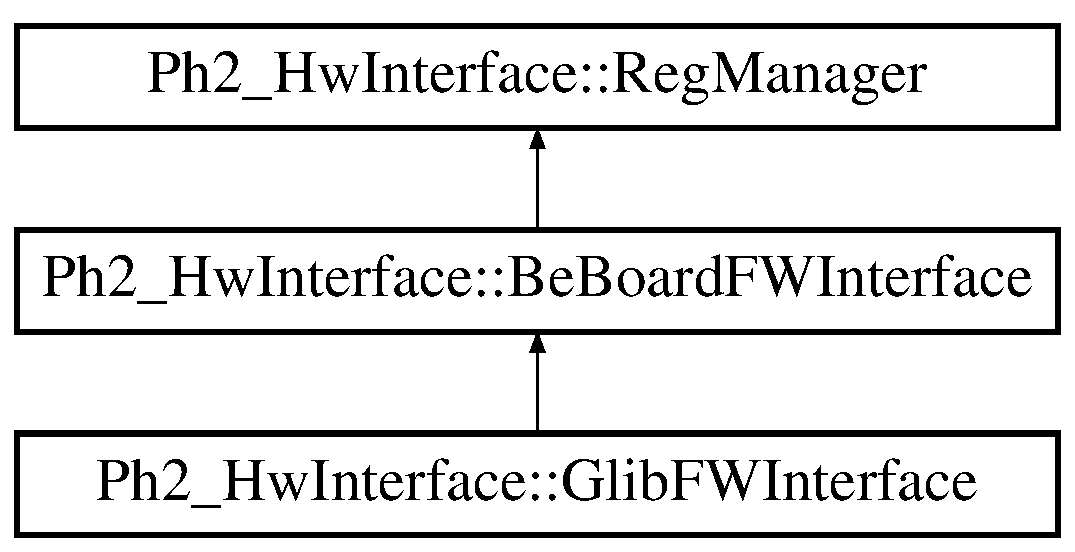
\includegraphics[height=3.000000cm]{class_ph2___hw_interface_1_1_be_board_f_w_interface}
\end{center}
\end{figure}
\subsection*{Public Member Functions}
\begin{DoxyCompactItemize}
\item 
\hyperlink{class_ph2___hw_interface_1_1_be_board_f_w_interface_a6a6be2907a3f6494422abb3ae2b35bd1}{Be\-Board\-F\-W\-Interface} (const char $\ast$pu\-Hal\-Config\-File\-Name, uint32\-\_\-t p\-Board\-Id)
\begin{DoxyCompactList}\small\item\em Constructor of the \hyperlink{class_ph2___hw_interface_1_1_be_board_f_w_interface}{Be\-Board\-F\-W\-Interface} class. \end{DoxyCompactList}\item 
virtual \hyperlink{class_ph2___hw_interface_1_1_be_board_f_w_interface_a22077ee1db6eb5ae149165bff88b5fa0}{$\sim$\-Be\-Board\-F\-W\-Interface} ()
\begin{DoxyCompactList}\small\item\em Destructor of the \hyperlink{class_ph2___hw_interface_1_1_be_board_f_w_interface}{Be\-Board\-F\-W\-Interface} class. \end{DoxyCompactList}\item 
virtual void \hyperlink{class_ph2___hw_interface_1_1_be_board_f_w_interface_aa93b2f84ca29ea20053fb42e5c8f3bb0}{define\-Event\-Size} (uint32\-\_\-t p\-Nb\-Cbc)
\begin{DoxyCompactList}\small\item\em Get the board infos. \end{DoxyCompactList}\item 
virtual std\-::string \hyperlink{class_ph2___hw_interface_1_1_be_board_f_w_interface_a895bb5ac8dfb81a00a047a6d8f5281b2}{get\-Board\-Type} ()
\begin{DoxyCompactList}\small\item\em Get the board type. \end{DoxyCompactList}\item 
virtual void \hyperlink{class_ph2___hw_interface_1_1_be_board_f_w_interface_a717caf9d29d3a7e92efceae18ad1dd78}{get\-Board\-Info} ()
\begin{DoxyCompactList}\small\item\em Get the board infos. \end{DoxyCompactList}\item 
virtual void \hyperlink{class_ph2___hw_interface_1_1_be_board_f_w_interface_ad19ee1309003c559db472046af4620d5}{Flash\-Prom} ()
\item 
virtual void \hyperlink{class_ph2___hw_interface_1_1_be_board_f_w_interface_a9575de192b6dd5613857ce255ec6947b}{Program\-Cdce} ()
\item 
virtual void \hyperlink{class_ph2___hw_interface_1_1_be_board_f_w_interface_a11f16d760d3e3df44daec200ac8d4275}{Encode\-Reg} (\hyperlink{struct_ph2___hw_description_1_1_cbc_reg_item}{Cbc\-Reg\-Item} \&p\-Reg\-Item, uint8\-\_\-t \&p\-Cbc\-Id, std\-::vector$<$ uint32\-\_\-t $>$ \&p\-Vec\-Req)
\begin{DoxyCompactList}\small\item\em Encode a/several word(s) readable for a Cbc. \end{DoxyCompactList}\item 
virtual void \hyperlink{class_ph2___hw_interface_1_1_be_board_f_w_interface_a31041cc7eee33af5663c035b88f5749c}{Decode\-Reg} (\hyperlink{struct_ph2___hw_description_1_1_cbc_reg_item}{Cbc\-Reg\-Item} \&p\-Reg\-Item, uint8\-\_\-t \&p\-Cbc\-Id, uint32\-\_\-t p\-Word)
\begin{DoxyCompactList}\small\item\em Decode a word from a read of a register of the Cbc. \end{DoxyCompactList}\item 
virtual void \hyperlink{class_ph2___hw_interface_1_1_be_board_f_w_interface_abfda233c55aaa85fcd3773fa424764d5}{Write\-Cbc\-Block\-Reg} (uint8\-\_\-t \&p\-Fe\-Id, std\-::vector$<$ uint32\-\_\-t $>$ \&p\-Vec\-Req)
\begin{DoxyCompactList}\small\item\em Write register blocks of a Cbc. \end{DoxyCompactList}\item 
virtual void \hyperlink{class_ph2___hw_interface_1_1_be_board_f_w_interface_aef5cfbb0b5adceff7ccc6babd3d01642}{Read\-Cbc\-Block\-Reg} (uint8\-\_\-t \&p\-Fe\-Id, std\-::vector$<$ uint32\-\_\-t $>$ \&p\-Vec\-Req)
\begin{DoxyCompactList}\small\item\em Read register blocks of a Cbc. \end{DoxyCompactList}\item 
virtual void \hyperlink{class_ph2___hw_interface_1_1_be_board_f_w_interface_a2507c664f19d1d5e3f6de69da16365e8}{Configure\-Board} (\hyperlink{class_ph2___hw_description_1_1_be_board}{Be\-Board} $\ast$p\-Board)
\begin{DoxyCompactList}\small\item\em Configure the board with its Config File. \end{DoxyCompactList}\item 
virtual void \hyperlink{class_ph2___hw_interface_1_1_be_board_f_w_interface_a2835dae7ec6788c1d5728e53f9c3051a}{Start} ()
\begin{DoxyCompactList}\small\item\em Start a D\-A\-Q. \end{DoxyCompactList}\item 
virtual void \hyperlink{class_ph2___hw_interface_1_1_be_board_f_w_interface_af7825e291796f7c8c498a92365583e08}{Stop} (uint32\-\_\-t p\-Nth\-Acq)
\begin{DoxyCompactList}\small\item\em Stop a D\-A\-Q. \end{DoxyCompactList}\item 
virtual void \hyperlink{class_ph2___hw_interface_1_1_be_board_f_w_interface_afb21d1663b328272c12cab6970114ecd}{Pause} ()
\begin{DoxyCompactList}\small\item\em Pause a D\-A\-Q. \end{DoxyCompactList}\item 
virtual void \hyperlink{class_ph2___hw_interface_1_1_be_board_f_w_interface_aafa48fcae2c37040141afc89113881e5}{Resume} ()
\begin{DoxyCompactList}\small\item\em Unpause a D\-A\-Q. \end{DoxyCompactList}\item 
virtual void \hyperlink{class_ph2___hw_interface_1_1_be_board_f_w_interface_af27f2a01b7625d2b144760413128acf2}{Read\-Data} (\hyperlink{class_ph2___hw_description_1_1_be_board}{Be\-Board} $\ast$p\-Board, uint32\-\_\-t p\-Nth\-Acq, bool p\-Break\-Trigger)
\begin{DoxyCompactList}\small\item\em Read data from D\-A\-Q. \end{DoxyCompactList}\item 
virtual const \hyperlink{class_ph2___hw_interface_1_1_event}{Event} $\ast$ \hyperlink{class_ph2___hw_interface_1_1_be_board_f_w_interface_a5f524d2a377db09667de71563e0fab3d}{Get\-Next\-Event} ()
\begin{DoxyCompactList}\small\item\em Get next event from data buffer. \end{DoxyCompactList}\item 
virtual const char $\ast$ \hyperlink{class_ph2___hw_interface_1_1_be_board_f_w_interface_aa298116ba4220d37f3eabfd57b0310c7}{Get\-Buffer} (uint32\-\_\-t \&p\-Buf\-Size)
\begin{DoxyCompactList}\small\item\em Get the data buffer. \end{DoxyCompactList}\end{DoxyCompactItemize}
\subsection*{Data Fields}
\begin{DoxyCompactItemize}
\item 
unsigned int \hyperlink{class_ph2___hw_interface_1_1_be_board_f_w_interface_a9cc80365ec331732245553a8bc0024ab}{f\-N\-Total\-Acq}
\item 
bool \hyperlink{class_ph2___hw_interface_1_1_be_board_f_w_interface_a2eae0dd93411d8acec67a41bcc09339b}{f\-Stop}
\item 
std\-::ofstream $\ast$ \hyperlink{class_ph2___hw_interface_1_1_be_board_f_w_interface_afa2f1748f8a2d527961766449cd91386}{f\-Data\-File}
\item 
\hyperlink{class_ph2___hw_interface_1_1_data}{Data} $\ast$ \hyperlink{class_ph2___hw_interface_1_1_be_board_f_w_interface_a9b315d4b61df34d093ed35cfef755a0f}{f\-Data}
\end{DoxyCompactItemize}
\subsection*{Additional Inherited Members}


\subsection{Detailed Description}
Class separating board system F\-W interface from u\-Hal wrapper. 

\subsection{Constructor \& Destructor Documentation}
\hypertarget{class_ph2___hw_interface_1_1_be_board_f_w_interface_a6a6be2907a3f6494422abb3ae2b35bd1}{\index{Ph2\-\_\-\-Hw\-Interface\-::\-Be\-Board\-F\-W\-Interface@{Ph2\-\_\-\-Hw\-Interface\-::\-Be\-Board\-F\-W\-Interface}!Be\-Board\-F\-W\-Interface@{Be\-Board\-F\-W\-Interface}}
\index{Be\-Board\-F\-W\-Interface@{Be\-Board\-F\-W\-Interface}!Ph2_HwInterface::BeBoardFWInterface@{Ph2\-\_\-\-Hw\-Interface\-::\-Be\-Board\-F\-W\-Interface}}
\subsubsection[{Be\-Board\-F\-W\-Interface}]{\setlength{\rightskip}{0pt plus 5cm}Ph2\-\_\-\-Hw\-Interface\-::\-Be\-Board\-F\-W\-Interface\-::\-Be\-Board\-F\-W\-Interface (
\begin{DoxyParamCaption}
\item[{const char $\ast$}]{pu\-Hal\-Config\-File\-Name, }
\item[{uint32\-\_\-t}]{p\-Board\-Id}
\end{DoxyParamCaption}
)}}\label{class_ph2___hw_interface_1_1_be_board_f_w_interface_a6a6be2907a3f6494422abb3ae2b35bd1}


Constructor of the \hyperlink{class_ph2___hw_interface_1_1_be_board_f_w_interface}{Be\-Board\-F\-W\-Interface} class. 


\begin{DoxyParams}{Parameters}
{\em pu\-Hal\-Config\-File\-Name} & \-: path of the u\-Hal Config File \\
\hline
\end{DoxyParams}
\hypertarget{class_ph2___hw_interface_1_1_be_board_f_w_interface_a22077ee1db6eb5ae149165bff88b5fa0}{\index{Ph2\-\_\-\-Hw\-Interface\-::\-Be\-Board\-F\-W\-Interface@{Ph2\-\_\-\-Hw\-Interface\-::\-Be\-Board\-F\-W\-Interface}!$\sim$\-Be\-Board\-F\-W\-Interface@{$\sim$\-Be\-Board\-F\-W\-Interface}}
\index{$\sim$\-Be\-Board\-F\-W\-Interface@{$\sim$\-Be\-Board\-F\-W\-Interface}!Ph2_HwInterface::BeBoardFWInterface@{Ph2\-\_\-\-Hw\-Interface\-::\-Be\-Board\-F\-W\-Interface}}
\subsubsection[{$\sim$\-Be\-Board\-F\-W\-Interface}]{\setlength{\rightskip}{0pt plus 5cm}Ph2\-\_\-\-Hw\-Interface\-::\-Be\-Board\-F\-W\-Interface\-::$\sim$\-Be\-Board\-F\-W\-Interface (
\begin{DoxyParamCaption}
{}
\end{DoxyParamCaption}
)\hspace{0.3cm}{\ttfamily [virtual]}}}\label{class_ph2___hw_interface_1_1_be_board_f_w_interface_a22077ee1db6eb5ae149165bff88b5fa0}


Destructor of the \hyperlink{class_ph2___hw_interface_1_1_be_board_f_w_interface}{Be\-Board\-F\-W\-Interface} class. 



\subsection{Member Function Documentation}
\hypertarget{class_ph2___hw_interface_1_1_be_board_f_w_interface_a2507c664f19d1d5e3f6de69da16365e8}{\index{Ph2\-\_\-\-Hw\-Interface\-::\-Be\-Board\-F\-W\-Interface@{Ph2\-\_\-\-Hw\-Interface\-::\-Be\-Board\-F\-W\-Interface}!Configure\-Board@{Configure\-Board}}
\index{Configure\-Board@{Configure\-Board}!Ph2_HwInterface::BeBoardFWInterface@{Ph2\-\_\-\-Hw\-Interface\-::\-Be\-Board\-F\-W\-Interface}}
\subsubsection[{Configure\-Board}]{\setlength{\rightskip}{0pt plus 5cm}virtual void Ph2\-\_\-\-Hw\-Interface\-::\-Be\-Board\-F\-W\-Interface\-::\-Configure\-Board (
\begin{DoxyParamCaption}
\item[{{\bf Be\-Board} $\ast$}]{p\-Board}
\end{DoxyParamCaption}
)\hspace{0.3cm}{\ttfamily [inline]}, {\ttfamily [virtual]}}}\label{class_ph2___hw_interface_1_1_be_board_f_w_interface_a2507c664f19d1d5e3f6de69da16365e8}


Configure the board with its Config File. 


\begin{DoxyParams}{Parameters}
{\em p\-Board} & \\
\hline
\end{DoxyParams}


Reimplemented in \hyperlink{class_ph2___hw_interface_1_1_glib_f_w_interface_a52658cd813658d4fae48a79bdabaa5cc}{Ph2\-\_\-\-Hw\-Interface\-::\-Glib\-F\-W\-Interface}.

\hypertarget{class_ph2___hw_interface_1_1_be_board_f_w_interface_a31041cc7eee33af5663c035b88f5749c}{\index{Ph2\-\_\-\-Hw\-Interface\-::\-Be\-Board\-F\-W\-Interface@{Ph2\-\_\-\-Hw\-Interface\-::\-Be\-Board\-F\-W\-Interface}!Decode\-Reg@{Decode\-Reg}}
\index{Decode\-Reg@{Decode\-Reg}!Ph2_HwInterface::BeBoardFWInterface@{Ph2\-\_\-\-Hw\-Interface\-::\-Be\-Board\-F\-W\-Interface}}
\subsubsection[{Decode\-Reg}]{\setlength{\rightskip}{0pt plus 5cm}void Ph2\-\_\-\-Hw\-Interface\-::\-Be\-Board\-F\-W\-Interface\-::\-Decode\-Reg (
\begin{DoxyParamCaption}
\item[{{\bf Cbc\-Reg\-Item} \&}]{p\-Reg\-Item, }
\item[{uint8\-\_\-t \&}]{p\-Cbc\-Id, }
\item[{uint32\-\_\-t}]{p\-Word}
\end{DoxyParamCaption}
)\hspace{0.3cm}{\ttfamily [virtual]}}}\label{class_ph2___hw_interface_1_1_be_board_f_w_interface_a31041cc7eee33af5663c035b88f5749c}


Decode a word from a read of a register of the Cbc. 


\begin{DoxyParams}{Parameters}
{\em p\-Reg\-Item} & \-: Reg\-Item containing infos (name, adress, value...) about the register to read \\
\hline
{\em p\-Cbc\-Id} & \-: Id of the Cbc to work with \\
\hline
{\em p\-Word} & \-: variable to put the decoded word\-Decode a word from a read of a register of the Cbc \\
\hline
\end{DoxyParams}
\hypertarget{class_ph2___hw_interface_1_1_be_board_f_w_interface_aa93b2f84ca29ea20053fb42e5c8f3bb0}{\index{Ph2\-\_\-\-Hw\-Interface\-::\-Be\-Board\-F\-W\-Interface@{Ph2\-\_\-\-Hw\-Interface\-::\-Be\-Board\-F\-W\-Interface}!define\-Event\-Size@{define\-Event\-Size}}
\index{define\-Event\-Size@{define\-Event\-Size}!Ph2_HwInterface::BeBoardFWInterface@{Ph2\-\_\-\-Hw\-Interface\-::\-Be\-Board\-F\-W\-Interface}}
\subsubsection[{define\-Event\-Size}]{\setlength{\rightskip}{0pt plus 5cm}void Ph2\-\_\-\-Hw\-Interface\-::\-Be\-Board\-F\-W\-Interface\-::define\-Event\-Size (
\begin{DoxyParamCaption}
\item[{uint32\-\_\-t}]{p\-Nb\-Cbc}
\end{DoxyParamCaption}
)\hspace{0.3cm}{\ttfamily [virtual]}}}\label{class_ph2___hw_interface_1_1_be_board_f_w_interface_aa93b2f84ca29ea20053fb42e5c8f3bb0}


Get the board infos. 


\begin{DoxyParams}{Parameters}
{\em p\-Board} & \\
\hline
\end{DoxyParams}
\hypertarget{class_ph2___hw_interface_1_1_be_board_f_w_interface_a11f16d760d3e3df44daec200ac8d4275}{\index{Ph2\-\_\-\-Hw\-Interface\-::\-Be\-Board\-F\-W\-Interface@{Ph2\-\_\-\-Hw\-Interface\-::\-Be\-Board\-F\-W\-Interface}!Encode\-Reg@{Encode\-Reg}}
\index{Encode\-Reg@{Encode\-Reg}!Ph2_HwInterface::BeBoardFWInterface@{Ph2\-\_\-\-Hw\-Interface\-::\-Be\-Board\-F\-W\-Interface}}
\subsubsection[{Encode\-Reg}]{\setlength{\rightskip}{0pt plus 5cm}void Ph2\-\_\-\-Hw\-Interface\-::\-Be\-Board\-F\-W\-Interface\-::\-Encode\-Reg (
\begin{DoxyParamCaption}
\item[{{\bf Cbc\-Reg\-Item} \&}]{p\-Reg\-Item, }
\item[{uint8\-\_\-t \&}]{p\-Cbc\-Id, }
\item[{std\-::vector$<$ uint32\-\_\-t $>$ \&}]{p\-Vec\-Req}
\end{DoxyParamCaption}
)\hspace{0.3cm}{\ttfamily [virtual]}}}\label{class_ph2___hw_interface_1_1_be_board_f_w_interface_a11f16d760d3e3df44daec200ac8d4275}


Encode a/several word(s) readable for a Cbc. 


\begin{DoxyParams}{Parameters}
{\em p\-Reg\-Item} & \-: Reg\-Item containing infos (name, adress, value...) about the register to write \\
\hline
{\em p\-Cbc\-Id} & \-: Id of the Cbc to work with \\
\hline
{\em p\-Vec\-Req} & \-: Vector to stack the encoded words\-Encode a/several word(s) readable for a Cbc \\
\hline
\end{DoxyParams}
\hypertarget{class_ph2___hw_interface_1_1_be_board_f_w_interface_ad19ee1309003c559db472046af4620d5}{\index{Ph2\-\_\-\-Hw\-Interface\-::\-Be\-Board\-F\-W\-Interface@{Ph2\-\_\-\-Hw\-Interface\-::\-Be\-Board\-F\-W\-Interface}!Flash\-Prom@{Flash\-Prom}}
\index{Flash\-Prom@{Flash\-Prom}!Ph2_HwInterface::BeBoardFWInterface@{Ph2\-\_\-\-Hw\-Interface\-::\-Be\-Board\-F\-W\-Interface}}
\subsubsection[{Flash\-Prom}]{\setlength{\rightskip}{0pt plus 5cm}virtual void Ph2\-\_\-\-Hw\-Interface\-::\-Be\-Board\-F\-W\-Interface\-::\-Flash\-Prom (
\begin{DoxyParamCaption}
{}
\end{DoxyParamCaption}
)\hspace{0.3cm}{\ttfamily [inline]}, {\ttfamily [virtual]}}}\label{class_ph2___hw_interface_1_1_be_board_f_w_interface_ad19ee1309003c559db472046af4620d5}
\hypertarget{class_ph2___hw_interface_1_1_be_board_f_w_interface_a717caf9d29d3a7e92efceae18ad1dd78}{\index{Ph2\-\_\-\-Hw\-Interface\-::\-Be\-Board\-F\-W\-Interface@{Ph2\-\_\-\-Hw\-Interface\-::\-Be\-Board\-F\-W\-Interface}!get\-Board\-Info@{get\-Board\-Info}}
\index{get\-Board\-Info@{get\-Board\-Info}!Ph2_HwInterface::BeBoardFWInterface@{Ph2\-\_\-\-Hw\-Interface\-::\-Be\-Board\-F\-W\-Interface}}
\subsubsection[{get\-Board\-Info}]{\setlength{\rightskip}{0pt plus 5cm}void Ph2\-\_\-\-Hw\-Interface\-::\-Be\-Board\-F\-W\-Interface\-::get\-Board\-Info (
\begin{DoxyParamCaption}
{}
\end{DoxyParamCaption}
)\hspace{0.3cm}{\ttfamily [virtual]}}}\label{class_ph2___hw_interface_1_1_be_board_f_w_interface_a717caf9d29d3a7e92efceae18ad1dd78}


Get the board infos. 


\begin{DoxyParams}{Parameters}
{\em p\-Board} & \\
\hline
\end{DoxyParams}
\hypertarget{class_ph2___hw_interface_1_1_be_board_f_w_interface_a895bb5ac8dfb81a00a047a6d8f5281b2}{\index{Ph2\-\_\-\-Hw\-Interface\-::\-Be\-Board\-F\-W\-Interface@{Ph2\-\_\-\-Hw\-Interface\-::\-Be\-Board\-F\-W\-Interface}!get\-Board\-Type@{get\-Board\-Type}}
\index{get\-Board\-Type@{get\-Board\-Type}!Ph2_HwInterface::BeBoardFWInterface@{Ph2\-\_\-\-Hw\-Interface\-::\-Be\-Board\-F\-W\-Interface}}
\subsubsection[{get\-Board\-Type}]{\setlength{\rightskip}{0pt plus 5cm}std\-::string Ph2\-\_\-\-Hw\-Interface\-::\-Be\-Board\-F\-W\-Interface\-::get\-Board\-Type (
\begin{DoxyParamCaption}
{}
\end{DoxyParamCaption}
)\hspace{0.3cm}{\ttfamily [virtual]}}}\label{class_ph2___hw_interface_1_1_be_board_f_w_interface_a895bb5ac8dfb81a00a047a6d8f5281b2}


Get the board type. 


\begin{DoxyParams}{Parameters}
{\em p\-Board} & \\
\hline
\end{DoxyParams}
\hypertarget{class_ph2___hw_interface_1_1_be_board_f_w_interface_aa298116ba4220d37f3eabfd57b0310c7}{\index{Ph2\-\_\-\-Hw\-Interface\-::\-Be\-Board\-F\-W\-Interface@{Ph2\-\_\-\-Hw\-Interface\-::\-Be\-Board\-F\-W\-Interface}!Get\-Buffer@{Get\-Buffer}}
\index{Get\-Buffer@{Get\-Buffer}!Ph2_HwInterface::BeBoardFWInterface@{Ph2\-\_\-\-Hw\-Interface\-::\-Be\-Board\-F\-W\-Interface}}
\subsubsection[{Get\-Buffer}]{\setlength{\rightskip}{0pt plus 5cm}virtual const char$\ast$ Ph2\-\_\-\-Hw\-Interface\-::\-Be\-Board\-F\-W\-Interface\-::\-Get\-Buffer (
\begin{DoxyParamCaption}
\item[{uint32\-\_\-t \&}]{p\-Buf\-Size}
\end{DoxyParamCaption}
)\hspace{0.3cm}{\ttfamily [inline]}, {\ttfamily [virtual]}}}\label{class_ph2___hw_interface_1_1_be_board_f_w_interface_aa298116ba4220d37f3eabfd57b0310c7}


Get the data buffer. 


\begin{DoxyParams}{Parameters}
{\em p\-Buf\-Size} & \-: recovers the data buffer size \\
\hline
\end{DoxyParams}
\begin{DoxyReturn}{Returns}
\hyperlink{class_ph2___hw_interface_1_1_data}{Data} buffer 
\end{DoxyReturn}


Reimplemented in \hyperlink{class_ph2___hw_interface_1_1_glib_f_w_interface_abd15e45762db510cdc41e039dabaab6c}{Ph2\-\_\-\-Hw\-Interface\-::\-Glib\-F\-W\-Interface}.

\hypertarget{class_ph2___hw_interface_1_1_be_board_f_w_interface_a5f524d2a377db09667de71563e0fab3d}{\index{Ph2\-\_\-\-Hw\-Interface\-::\-Be\-Board\-F\-W\-Interface@{Ph2\-\_\-\-Hw\-Interface\-::\-Be\-Board\-F\-W\-Interface}!Get\-Next\-Event@{Get\-Next\-Event}}
\index{Get\-Next\-Event@{Get\-Next\-Event}!Ph2_HwInterface::BeBoardFWInterface@{Ph2\-\_\-\-Hw\-Interface\-::\-Be\-Board\-F\-W\-Interface}}
\subsubsection[{Get\-Next\-Event}]{\setlength{\rightskip}{0pt plus 5cm}virtual const {\bf Event}$\ast$ Ph2\-\_\-\-Hw\-Interface\-::\-Be\-Board\-F\-W\-Interface\-::\-Get\-Next\-Event (
\begin{DoxyParamCaption}
{}
\end{DoxyParamCaption}
)\hspace{0.3cm}{\ttfamily [inline]}, {\ttfamily [virtual]}}}\label{class_ph2___hw_interface_1_1_be_board_f_w_interface_a5f524d2a377db09667de71563e0fab3d}


Get next event from data buffer. 

\begin{DoxyReturn}{Returns}
Next event 
\end{DoxyReturn}


Reimplemented in \hyperlink{class_ph2___hw_interface_1_1_glib_f_w_interface_afebeee20cd186f919189e5f349c6a49f}{Ph2\-\_\-\-Hw\-Interface\-::\-Glib\-F\-W\-Interface}.

\hypertarget{class_ph2___hw_interface_1_1_be_board_f_w_interface_afb21d1663b328272c12cab6970114ecd}{\index{Ph2\-\_\-\-Hw\-Interface\-::\-Be\-Board\-F\-W\-Interface@{Ph2\-\_\-\-Hw\-Interface\-::\-Be\-Board\-F\-W\-Interface}!Pause@{Pause}}
\index{Pause@{Pause}!Ph2_HwInterface::BeBoardFWInterface@{Ph2\-\_\-\-Hw\-Interface\-::\-Be\-Board\-F\-W\-Interface}}
\subsubsection[{Pause}]{\setlength{\rightskip}{0pt plus 5cm}virtual void Ph2\-\_\-\-Hw\-Interface\-::\-Be\-Board\-F\-W\-Interface\-::\-Pause (
\begin{DoxyParamCaption}
{}
\end{DoxyParamCaption}
)\hspace{0.3cm}{\ttfamily [inline]}, {\ttfamily [virtual]}}}\label{class_ph2___hw_interface_1_1_be_board_f_w_interface_afb21d1663b328272c12cab6970114ecd}


Pause a D\-A\-Q. 


\begin{DoxyParams}{Parameters}
{\em p\-Board} & \\
\hline
\end{DoxyParams}


Reimplemented in \hyperlink{class_ph2___hw_interface_1_1_glib_f_w_interface_a05d7f790e0316b51714293e8089086f3}{Ph2\-\_\-\-Hw\-Interface\-::\-Glib\-F\-W\-Interface}.

\hypertarget{class_ph2___hw_interface_1_1_be_board_f_w_interface_a9575de192b6dd5613857ce255ec6947b}{\index{Ph2\-\_\-\-Hw\-Interface\-::\-Be\-Board\-F\-W\-Interface@{Ph2\-\_\-\-Hw\-Interface\-::\-Be\-Board\-F\-W\-Interface}!Program\-Cdce@{Program\-Cdce}}
\index{Program\-Cdce@{Program\-Cdce}!Ph2_HwInterface::BeBoardFWInterface@{Ph2\-\_\-\-Hw\-Interface\-::\-Be\-Board\-F\-W\-Interface}}
\subsubsection[{Program\-Cdce}]{\setlength{\rightskip}{0pt plus 5cm}virtual void Ph2\-\_\-\-Hw\-Interface\-::\-Be\-Board\-F\-W\-Interface\-::\-Program\-Cdce (
\begin{DoxyParamCaption}
{}
\end{DoxyParamCaption}
)\hspace{0.3cm}{\ttfamily [inline]}, {\ttfamily [virtual]}}}\label{class_ph2___hw_interface_1_1_be_board_f_w_interface_a9575de192b6dd5613857ce255ec6947b}
\hypertarget{class_ph2___hw_interface_1_1_be_board_f_w_interface_aef5cfbb0b5adceff7ccc6babd3d01642}{\index{Ph2\-\_\-\-Hw\-Interface\-::\-Be\-Board\-F\-W\-Interface@{Ph2\-\_\-\-Hw\-Interface\-::\-Be\-Board\-F\-W\-Interface}!Read\-Cbc\-Block\-Reg@{Read\-Cbc\-Block\-Reg}}
\index{Read\-Cbc\-Block\-Reg@{Read\-Cbc\-Block\-Reg}!Ph2_HwInterface::BeBoardFWInterface@{Ph2\-\_\-\-Hw\-Interface\-::\-Be\-Board\-F\-W\-Interface}}
\subsubsection[{Read\-Cbc\-Block\-Reg}]{\setlength{\rightskip}{0pt plus 5cm}virtual void Ph2\-\_\-\-Hw\-Interface\-::\-Be\-Board\-F\-W\-Interface\-::\-Read\-Cbc\-Block\-Reg (
\begin{DoxyParamCaption}
\item[{uint8\-\_\-t \&}]{p\-Fe\-Id, }
\item[{std\-::vector$<$ uint32\-\_\-t $>$ \&}]{p\-Vec\-Req}
\end{DoxyParamCaption}
)\hspace{0.3cm}{\ttfamily [inline]}, {\ttfamily [virtual]}}}\label{class_ph2___hw_interface_1_1_be_board_f_w_interface_aef5cfbb0b5adceff7ccc6babd3d01642}


Read register blocks of a Cbc. 


\begin{DoxyParams}{Parameters}
{\em p\-Cbc} & \-: Cbc to work with \\
\hline
{\em p\-Vec\-Req} & \-: Vector to stack the read words \\
\hline
\end{DoxyParams}


Reimplemented in \hyperlink{class_ph2___hw_interface_1_1_glib_f_w_interface_af1fc5669e98ae17f235c47f08ac256c0}{Ph2\-\_\-\-Hw\-Interface\-::\-Glib\-F\-W\-Interface}.

\hypertarget{class_ph2___hw_interface_1_1_be_board_f_w_interface_af27f2a01b7625d2b144760413128acf2}{\index{Ph2\-\_\-\-Hw\-Interface\-::\-Be\-Board\-F\-W\-Interface@{Ph2\-\_\-\-Hw\-Interface\-::\-Be\-Board\-F\-W\-Interface}!Read\-Data@{Read\-Data}}
\index{Read\-Data@{Read\-Data}!Ph2_HwInterface::BeBoardFWInterface@{Ph2\-\_\-\-Hw\-Interface\-::\-Be\-Board\-F\-W\-Interface}}
\subsubsection[{Read\-Data}]{\setlength{\rightskip}{0pt plus 5cm}virtual void Ph2\-\_\-\-Hw\-Interface\-::\-Be\-Board\-F\-W\-Interface\-::\-Read\-Data (
\begin{DoxyParamCaption}
\item[{{\bf Be\-Board} $\ast$}]{p\-Board, }
\item[{uint32\-\_\-t}]{p\-Nth\-Acq, }
\item[{bool}]{p\-Break\-Trigger}
\end{DoxyParamCaption}
)\hspace{0.3cm}{\ttfamily [inline]}, {\ttfamily [virtual]}}}\label{class_ph2___hw_interface_1_1_be_board_f_w_interface_af27f2a01b7625d2b144760413128acf2}


Read data from D\-A\-Q. 


\begin{DoxyParams}{Parameters}
{\em p\-Board} & \\
\hline
{\em p\-Nth\-Acq} & \-: actual number of acquisitions \\
\hline
{\em p\-Break\-Trigger} & \-: if true, enable the break trigger \\
\hline
\end{DoxyParams}


Reimplemented in \hyperlink{class_ph2___hw_interface_1_1_glib_f_w_interface_a26c35fec3518f40d09ebc7f0114be19b}{Ph2\-\_\-\-Hw\-Interface\-::\-Glib\-F\-W\-Interface}.

\hypertarget{class_ph2___hw_interface_1_1_be_board_f_w_interface_aafa48fcae2c37040141afc89113881e5}{\index{Ph2\-\_\-\-Hw\-Interface\-::\-Be\-Board\-F\-W\-Interface@{Ph2\-\_\-\-Hw\-Interface\-::\-Be\-Board\-F\-W\-Interface}!Resume@{Resume}}
\index{Resume@{Resume}!Ph2_HwInterface::BeBoardFWInterface@{Ph2\-\_\-\-Hw\-Interface\-::\-Be\-Board\-F\-W\-Interface}}
\subsubsection[{Resume}]{\setlength{\rightskip}{0pt plus 5cm}virtual void Ph2\-\_\-\-Hw\-Interface\-::\-Be\-Board\-F\-W\-Interface\-::\-Resume (
\begin{DoxyParamCaption}
{}
\end{DoxyParamCaption}
)\hspace{0.3cm}{\ttfamily [inline]}, {\ttfamily [virtual]}}}\label{class_ph2___hw_interface_1_1_be_board_f_w_interface_aafa48fcae2c37040141afc89113881e5}


Unpause a D\-A\-Q. 


\begin{DoxyParams}{Parameters}
{\em p\-Board} & \\
\hline
\end{DoxyParams}


Reimplemented in \hyperlink{class_ph2___hw_interface_1_1_glib_f_w_interface_aedd3abfb576016701da27fabc975ac13}{Ph2\-\_\-\-Hw\-Interface\-::\-Glib\-F\-W\-Interface}.

\hypertarget{class_ph2___hw_interface_1_1_be_board_f_w_interface_a2835dae7ec6788c1d5728e53f9c3051a}{\index{Ph2\-\_\-\-Hw\-Interface\-::\-Be\-Board\-F\-W\-Interface@{Ph2\-\_\-\-Hw\-Interface\-::\-Be\-Board\-F\-W\-Interface}!Start@{Start}}
\index{Start@{Start}!Ph2_HwInterface::BeBoardFWInterface@{Ph2\-\_\-\-Hw\-Interface\-::\-Be\-Board\-F\-W\-Interface}}
\subsubsection[{Start}]{\setlength{\rightskip}{0pt plus 5cm}virtual void Ph2\-\_\-\-Hw\-Interface\-::\-Be\-Board\-F\-W\-Interface\-::\-Start (
\begin{DoxyParamCaption}
{}
\end{DoxyParamCaption}
)\hspace{0.3cm}{\ttfamily [inline]}, {\ttfamily [virtual]}}}\label{class_ph2___hw_interface_1_1_be_board_f_w_interface_a2835dae7ec6788c1d5728e53f9c3051a}


Start a D\-A\-Q. 


\begin{DoxyParams}{Parameters}
{\em p\-Board} & \\
\hline
\end{DoxyParams}


Reimplemented in \hyperlink{class_ph2___hw_interface_1_1_glib_f_w_interface_adebd47ee3a84dbb8b60f6dd521921aac}{Ph2\-\_\-\-Hw\-Interface\-::\-Glib\-F\-W\-Interface}.

\hypertarget{class_ph2___hw_interface_1_1_be_board_f_w_interface_af7825e291796f7c8c498a92365583e08}{\index{Ph2\-\_\-\-Hw\-Interface\-::\-Be\-Board\-F\-W\-Interface@{Ph2\-\_\-\-Hw\-Interface\-::\-Be\-Board\-F\-W\-Interface}!Stop@{Stop}}
\index{Stop@{Stop}!Ph2_HwInterface::BeBoardFWInterface@{Ph2\-\_\-\-Hw\-Interface\-::\-Be\-Board\-F\-W\-Interface}}
\subsubsection[{Stop}]{\setlength{\rightskip}{0pt plus 5cm}virtual void Ph2\-\_\-\-Hw\-Interface\-::\-Be\-Board\-F\-W\-Interface\-::\-Stop (
\begin{DoxyParamCaption}
\item[{uint32\-\_\-t}]{p\-Nth\-Acq}
\end{DoxyParamCaption}
)\hspace{0.3cm}{\ttfamily [inline]}, {\ttfamily [virtual]}}}\label{class_ph2___hw_interface_1_1_be_board_f_w_interface_af7825e291796f7c8c498a92365583e08}


Stop a D\-A\-Q. 


\begin{DoxyParams}{Parameters}
{\em p\-Board} & \\
\hline
{\em p\-Nth\-Acq} & \-: actual number of acquisitions \\
\hline
\end{DoxyParams}


Reimplemented in \hyperlink{class_ph2___hw_interface_1_1_glib_f_w_interface_ad980b1ab04d9f87f1a26978201e42997}{Ph2\-\_\-\-Hw\-Interface\-::\-Glib\-F\-W\-Interface}.

\hypertarget{class_ph2___hw_interface_1_1_be_board_f_w_interface_abfda233c55aaa85fcd3773fa424764d5}{\index{Ph2\-\_\-\-Hw\-Interface\-::\-Be\-Board\-F\-W\-Interface@{Ph2\-\_\-\-Hw\-Interface\-::\-Be\-Board\-F\-W\-Interface}!Write\-Cbc\-Block\-Reg@{Write\-Cbc\-Block\-Reg}}
\index{Write\-Cbc\-Block\-Reg@{Write\-Cbc\-Block\-Reg}!Ph2_HwInterface::BeBoardFWInterface@{Ph2\-\_\-\-Hw\-Interface\-::\-Be\-Board\-F\-W\-Interface}}
\subsubsection[{Write\-Cbc\-Block\-Reg}]{\setlength{\rightskip}{0pt plus 5cm}virtual void Ph2\-\_\-\-Hw\-Interface\-::\-Be\-Board\-F\-W\-Interface\-::\-Write\-Cbc\-Block\-Reg (
\begin{DoxyParamCaption}
\item[{uint8\-\_\-t \&}]{p\-Fe\-Id, }
\item[{std\-::vector$<$ uint32\-\_\-t $>$ \&}]{p\-Vec\-Req}
\end{DoxyParamCaption}
)\hspace{0.3cm}{\ttfamily [inline]}, {\ttfamily [virtual]}}}\label{class_ph2___hw_interface_1_1_be_board_f_w_interface_abfda233c55aaa85fcd3773fa424764d5}


Write register blocks of a Cbc. 


\begin{DoxyParams}{Parameters}
{\em p\-Cbc} & \-: Cbc to work with \\
\hline
{\em p\-Vec\-Req} & \-: Block of words to write \\
\hline
\end{DoxyParams}


Reimplemented in \hyperlink{class_ph2___hw_interface_1_1_glib_f_w_interface_a1a43546404b9097fafa83302cd326e4c}{Ph2\-\_\-\-Hw\-Interface\-::\-Glib\-F\-W\-Interface}.



\subsection{Field Documentation}
\hypertarget{class_ph2___hw_interface_1_1_be_board_f_w_interface_a9b315d4b61df34d093ed35cfef755a0f}{\index{Ph2\-\_\-\-Hw\-Interface\-::\-Be\-Board\-F\-W\-Interface@{Ph2\-\_\-\-Hw\-Interface\-::\-Be\-Board\-F\-W\-Interface}!f\-Data@{f\-Data}}
\index{f\-Data@{f\-Data}!Ph2_HwInterface::BeBoardFWInterface@{Ph2\-\_\-\-Hw\-Interface\-::\-Be\-Board\-F\-W\-Interface}}
\subsubsection[{f\-Data}]{\setlength{\rightskip}{0pt plus 5cm}{\bf Data}$\ast$ Ph2\-\_\-\-Hw\-Interface\-::\-Be\-Board\-F\-W\-Interface\-::f\-Data}}\label{class_ph2___hw_interface_1_1_be_board_f_w_interface_a9b315d4b61df34d093ed35cfef755a0f}
\hyperlink{class_ph2___hw_interface_1_1_data}{Data} read storage \hypertarget{class_ph2___hw_interface_1_1_be_board_f_w_interface_afa2f1748f8a2d527961766449cd91386}{\index{Ph2\-\_\-\-Hw\-Interface\-::\-Be\-Board\-F\-W\-Interface@{Ph2\-\_\-\-Hw\-Interface\-::\-Be\-Board\-F\-W\-Interface}!f\-Data\-File@{f\-Data\-File}}
\index{f\-Data\-File@{f\-Data\-File}!Ph2_HwInterface::BeBoardFWInterface@{Ph2\-\_\-\-Hw\-Interface\-::\-Be\-Board\-F\-W\-Interface}}
\subsubsection[{f\-Data\-File}]{\setlength{\rightskip}{0pt plus 5cm}std\-::ofstream$\ast$ Ph2\-\_\-\-Hw\-Interface\-::\-Be\-Board\-F\-W\-Interface\-::f\-Data\-File}}\label{class_ph2___hw_interface_1_1_be_board_f_w_interface_afa2f1748f8a2d527961766449cd91386}
File storing data \hypertarget{class_ph2___hw_interface_1_1_be_board_f_w_interface_a9cc80365ec331732245553a8bc0024ab}{\index{Ph2\-\_\-\-Hw\-Interface\-::\-Be\-Board\-F\-W\-Interface@{Ph2\-\_\-\-Hw\-Interface\-::\-Be\-Board\-F\-W\-Interface}!f\-N\-Total\-Acq@{f\-N\-Total\-Acq}}
\index{f\-N\-Total\-Acq@{f\-N\-Total\-Acq}!Ph2_HwInterface::BeBoardFWInterface@{Ph2\-\_\-\-Hw\-Interface\-::\-Be\-Board\-F\-W\-Interface}}
\subsubsection[{f\-N\-Total\-Acq}]{\setlength{\rightskip}{0pt plus 5cm}unsigned int Ph2\-\_\-\-Hw\-Interface\-::\-Be\-Board\-F\-W\-Interface\-::f\-N\-Total\-Acq}}\label{class_ph2___hw_interface_1_1_be_board_f_w_interface_a9cc80365ec331732245553a8bc0024ab}
\hypertarget{class_ph2___hw_interface_1_1_be_board_f_w_interface_a2eae0dd93411d8acec67a41bcc09339b}{\index{Ph2\-\_\-\-Hw\-Interface\-::\-Be\-Board\-F\-W\-Interface@{Ph2\-\_\-\-Hw\-Interface\-::\-Be\-Board\-F\-W\-Interface}!f\-Stop@{f\-Stop}}
\index{f\-Stop@{f\-Stop}!Ph2_HwInterface::BeBoardFWInterface@{Ph2\-\_\-\-Hw\-Interface\-::\-Be\-Board\-F\-W\-Interface}}
\subsubsection[{f\-Stop}]{\setlength{\rightskip}{0pt plus 5cm}bool Ph2\-\_\-\-Hw\-Interface\-::\-Be\-Board\-F\-W\-Interface\-::f\-Stop}}\label{class_ph2___hw_interface_1_1_be_board_f_w_interface_a2eae0dd93411d8acec67a41bcc09339b}


The documentation for this class was generated from the following files\-:\begin{DoxyCompactItemize}
\item 
H\-W\-Interface/\hyperlink{_be_board_f_w_interface_8h}{Be\-Board\-F\-W\-Interface.\-h}\item 
H\-W\-Interface/\hyperlink{_be_board_f_w_interface_8cc}{Be\-Board\-F\-W\-Interface.\-cc}\end{DoxyCompactItemize}

\hypertarget{class_ph2___hw_interface_1_1_be_board_interface}{\section{Ph2\-\_\-\-Hw\-Interface\-:\-:Be\-Board\-Interface Class Reference}
\label{class_ph2___hw_interface_1_1_be_board_interface}\index{Ph2\-\_\-\-Hw\-Interface\-::\-Be\-Board\-Interface@{Ph2\-\_\-\-Hw\-Interface\-::\-Be\-Board\-Interface}}
}


Class representing the User Interface to the different boards.  




{\ttfamily \#include $<$Be\-Board\-Interface.\-h$>$}

\subsection*{Public Member Functions}
\begin{DoxyCompactItemize}
\item 
\hyperlink{class_ph2___hw_interface_1_1_be_board_interface_a621bd484157724e03eeba5d52ce0b726}{Be\-Board\-Interface} (\hyperlink{namespace_ph2___hw_interface_ac35d341eb47fa7cbe4d28ccbc6ab4875}{Be\-Board\-F\-W\-Map} \&p\-Board\-Map)
\begin{DoxyCompactList}\small\item\em Constructor of the \hyperlink{class_ph2___hw_interface_1_1_be_board_interface}{Be\-Board\-Interface} class. \end{DoxyCompactList}\item 
\hyperlink{class_ph2___hw_interface_1_1_be_board_interface_ad67b2d931b904565cf6e5881fa0d140e}{$\sim$\-Be\-Board\-Interface} ()
\begin{DoxyCompactList}\small\item\em Destructor of the \hyperlink{class_ph2___hw_interface_1_1_be_board_interface}{Be\-Board\-Interface} class. \end{DoxyCompactList}\item 
void \hyperlink{class_ph2___hw_interface_1_1_be_board_interface_add92a5f30e058c3a384b8fde1015f31a}{Write\-Board\-Reg} (\hyperlink{class_ph2___hw_description_1_1_be_board}{Be\-Board} $\ast$p\-Board, const std\-::string \&p\-Reg\-Node, const uint32\-\_\-t \&p\-Val)
\begin{DoxyCompactList}\small\item\em Update both Board register and Config File. \end{DoxyCompactList}\item 
void \hyperlink{class_ph2___hw_interface_1_1_be_board_interface_a1b3096f0b052d6e9329fdb3b9a8299fb}{Read\-Board\-Reg} (\hyperlink{class_ph2___hw_description_1_1_be_board}{Be\-Board} $\ast$p\-Board, const std\-::string \&p\-Reg\-Node)
\begin{DoxyCompactList}\small\item\em Update Config File with the value in the Board register. \end{DoxyCompactList}\item 
void \hyperlink{class_ph2___hw_interface_1_1_be_board_interface_ae423a6ec7526a0abd9ce3c9e0e3b1847}{get\-Board\-Info} (\hyperlink{class_ph2___hw_description_1_1_be_board}{Be\-Board} $\ast$p\-Board)
\begin{DoxyCompactList}\small\item\em Get the board infos. \end{DoxyCompactList}\item 
void \hyperlink{class_ph2___hw_interface_1_1_be_board_interface_a808eabcbd850dd651f9b3122f702079f}{Configure\-Board} (\hyperlink{class_ph2___hw_description_1_1_be_board}{Be\-Board} $\ast$p\-Board)
\begin{DoxyCompactList}\small\item\em Configure the board with its Config File. \end{DoxyCompactList}\item 
void \hyperlink{class_ph2___hw_interface_1_1_be_board_interface_ac78a16fd4779f86c1224b09d30349e18}{Start} (\hyperlink{class_ph2___hw_description_1_1_be_board}{Be\-Board} $\ast$p\-Board)
\begin{DoxyCompactList}\small\item\em Start a D\-A\-Q. \end{DoxyCompactList}\item 
void \hyperlink{class_ph2___hw_interface_1_1_be_board_interface_a08d0374efe31d8078f8d31f58b709e6f}{Stop} (\hyperlink{class_ph2___hw_description_1_1_be_board}{Be\-Board} $\ast$p\-Board, uint32\-\_\-t p\-Nth\-Acq)
\begin{DoxyCompactList}\small\item\em Stop a D\-A\-Q. \end{DoxyCompactList}\item 
void \hyperlink{class_ph2___hw_interface_1_1_be_board_interface_a2b9692f018d7756fbfd720224da542da}{Pause} (\hyperlink{class_ph2___hw_description_1_1_be_board}{Be\-Board} $\ast$p\-Board)
\begin{DoxyCompactList}\small\item\em Pause a D\-A\-Q. \end{DoxyCompactList}\item 
void \hyperlink{class_ph2___hw_interface_1_1_be_board_interface_ad21d2651379571889a7a2ebc55ee3223}{Resume} (\hyperlink{class_ph2___hw_description_1_1_be_board}{Be\-Board} $\ast$p\-Board)
\begin{DoxyCompactList}\small\item\em Unpause a D\-A\-Q. \end{DoxyCompactList}\item 
void \hyperlink{class_ph2___hw_interface_1_1_be_board_interface_a3e5106285fa795c21cb9d20fbf753759}{Read\-Data} (\hyperlink{class_ph2___hw_description_1_1_be_board}{Be\-Board} $\ast$p\-Board, uint32\-\_\-t p\-Nth\-Acq, bool p\-Break\-Trigger)
\begin{DoxyCompactList}\small\item\em Read data from D\-A\-Q. \end{DoxyCompactList}\item 
const \hyperlink{class_ph2___hw_interface_1_1_event}{Event} $\ast$ \hyperlink{class_ph2___hw_interface_1_1_be_board_interface_a8dadf0d6aba310d1476b5c50aae98742}{Get\-Next\-Event} (\hyperlink{class_ph2___hw_description_1_1_be_board}{Be\-Board} $\ast$p\-Board)
\begin{DoxyCompactList}\small\item\em Get next event from data buffer. \end{DoxyCompactList}\end{DoxyCompactItemize}
\subsection*{Private Member Functions}
\begin{DoxyCompactItemize}
\item 
void \hyperlink{class_ph2___hw_interface_1_1_be_board_interface_ac4f6fae0f69208acc832437359993665}{set\-Board} (uint8\-\_\-t p\-Board\-Id)
\begin{DoxyCompactList}\small\item\em Set the board to talk with. \end{DoxyCompactList}\end{DoxyCompactItemize}
\subsection*{Private Attributes}
\begin{DoxyCompactItemize}
\item 
\hyperlink{namespace_ph2___hw_interface_ac35d341eb47fa7cbe4d28ccbc6ab4875}{Be\-Board\-F\-W\-Map} \& \hyperlink{class_ph2___hw_interface_1_1_be_board_interface_aff153bb1272b1f145c919a9ba2cc572d}{f\-Board\-Map}
\item 
\hyperlink{class_ph2___hw_interface_1_1_be_board_f_w_interface}{Be\-Board\-F\-W\-Interface} $\ast$ \hyperlink{class_ph2___hw_interface_1_1_be_board_interface_a763c8be5545618fb5ca0dfe01667f9ae}{f\-Board\-F\-W}
\item 
uint8\-\_\-t \hyperlink{class_ph2___hw_interface_1_1_be_board_interface_af248fa0474f163d72349854f12d3ad61}{prev\-Board\-Id}
\end{DoxyCompactItemize}


\subsection{Detailed Description}
Class representing the User Interface to the different boards. 

\subsection{Constructor \& Destructor Documentation}
\hypertarget{class_ph2___hw_interface_1_1_be_board_interface_a621bd484157724e03eeba5d52ce0b726}{\index{Ph2\-\_\-\-Hw\-Interface\-::\-Be\-Board\-Interface@{Ph2\-\_\-\-Hw\-Interface\-::\-Be\-Board\-Interface}!Be\-Board\-Interface@{Be\-Board\-Interface}}
\index{Be\-Board\-Interface@{Be\-Board\-Interface}!Ph2_HwInterface::BeBoardInterface@{Ph2\-\_\-\-Hw\-Interface\-::\-Be\-Board\-Interface}}
\subsubsection[{Be\-Board\-Interface}]{\setlength{\rightskip}{0pt plus 5cm}Ph2\-\_\-\-Hw\-Interface\-::\-Be\-Board\-Interface\-::\-Be\-Board\-Interface (
\begin{DoxyParamCaption}
\item[{{\bf Be\-Board\-F\-W\-Map} \&}]{p\-Board\-Map}
\end{DoxyParamCaption}
)}}\label{class_ph2___hw_interface_1_1_be_board_interface_a621bd484157724e03eeba5d52ce0b726}


Constructor of the \hyperlink{class_ph2___hw_interface_1_1_be_board_interface}{Be\-Board\-Interface} class. 


\begin{DoxyParams}{Parameters}
{\em Reference} & to the Board\-F\-W\-Interface \\
\hline
\end{DoxyParams}
\hypertarget{class_ph2___hw_interface_1_1_be_board_interface_ad67b2d931b904565cf6e5881fa0d140e}{\index{Ph2\-\_\-\-Hw\-Interface\-::\-Be\-Board\-Interface@{Ph2\-\_\-\-Hw\-Interface\-::\-Be\-Board\-Interface}!$\sim$\-Be\-Board\-Interface@{$\sim$\-Be\-Board\-Interface}}
\index{$\sim$\-Be\-Board\-Interface@{$\sim$\-Be\-Board\-Interface}!Ph2_HwInterface::BeBoardInterface@{Ph2\-\_\-\-Hw\-Interface\-::\-Be\-Board\-Interface}}
\subsubsection[{$\sim$\-Be\-Board\-Interface}]{\setlength{\rightskip}{0pt plus 5cm}Ph2\-\_\-\-Hw\-Interface\-::\-Be\-Board\-Interface\-::$\sim$\-Be\-Board\-Interface (
\begin{DoxyParamCaption}
{}
\end{DoxyParamCaption}
)}}\label{class_ph2___hw_interface_1_1_be_board_interface_ad67b2d931b904565cf6e5881fa0d140e}


Destructor of the \hyperlink{class_ph2___hw_interface_1_1_be_board_interface}{Be\-Board\-Interface} class. 



\subsection{Member Function Documentation}
\hypertarget{class_ph2___hw_interface_1_1_be_board_interface_a808eabcbd850dd651f9b3122f702079f}{\index{Ph2\-\_\-\-Hw\-Interface\-::\-Be\-Board\-Interface@{Ph2\-\_\-\-Hw\-Interface\-::\-Be\-Board\-Interface}!Configure\-Board@{Configure\-Board}}
\index{Configure\-Board@{Configure\-Board}!Ph2_HwInterface::BeBoardInterface@{Ph2\-\_\-\-Hw\-Interface\-::\-Be\-Board\-Interface}}
\subsubsection[{Configure\-Board}]{\setlength{\rightskip}{0pt plus 5cm}void Ph2\-\_\-\-Hw\-Interface\-::\-Be\-Board\-Interface\-::\-Configure\-Board (
\begin{DoxyParamCaption}
\item[{{\bf Be\-Board} $\ast$}]{p\-Board}
\end{DoxyParamCaption}
)}}\label{class_ph2___hw_interface_1_1_be_board_interface_a808eabcbd850dd651f9b3122f702079f}


Configure the board with its Config File. 


\begin{DoxyParams}{Parameters}
{\em p\-Board} & \\
\hline
\end{DoxyParams}
\hypertarget{class_ph2___hw_interface_1_1_be_board_interface_ae423a6ec7526a0abd9ce3c9e0e3b1847}{\index{Ph2\-\_\-\-Hw\-Interface\-::\-Be\-Board\-Interface@{Ph2\-\_\-\-Hw\-Interface\-::\-Be\-Board\-Interface}!get\-Board\-Info@{get\-Board\-Info}}
\index{get\-Board\-Info@{get\-Board\-Info}!Ph2_HwInterface::BeBoardInterface@{Ph2\-\_\-\-Hw\-Interface\-::\-Be\-Board\-Interface}}
\subsubsection[{get\-Board\-Info}]{\setlength{\rightskip}{0pt plus 5cm}void Ph2\-\_\-\-Hw\-Interface\-::\-Be\-Board\-Interface\-::get\-Board\-Info (
\begin{DoxyParamCaption}
\item[{{\bf Be\-Board} $\ast$}]{p\-Board}
\end{DoxyParamCaption}
)}}\label{class_ph2___hw_interface_1_1_be_board_interface_ae423a6ec7526a0abd9ce3c9e0e3b1847}


Get the board infos. 


\begin{DoxyParams}{Parameters}
{\em p\-Board} & \\
\hline
\end{DoxyParams}
\hypertarget{class_ph2___hw_interface_1_1_be_board_interface_a8dadf0d6aba310d1476b5c50aae98742}{\index{Ph2\-\_\-\-Hw\-Interface\-::\-Be\-Board\-Interface@{Ph2\-\_\-\-Hw\-Interface\-::\-Be\-Board\-Interface}!Get\-Next\-Event@{Get\-Next\-Event}}
\index{Get\-Next\-Event@{Get\-Next\-Event}!Ph2_HwInterface::BeBoardInterface@{Ph2\-\_\-\-Hw\-Interface\-::\-Be\-Board\-Interface}}
\subsubsection[{Get\-Next\-Event}]{\setlength{\rightskip}{0pt plus 5cm}const {\bf Event} $\ast$ Ph2\-\_\-\-Hw\-Interface\-::\-Be\-Board\-Interface\-::\-Get\-Next\-Event (
\begin{DoxyParamCaption}
\item[{{\bf Be\-Board} $\ast$}]{p\-Board}
\end{DoxyParamCaption}
)}}\label{class_ph2___hw_interface_1_1_be_board_interface_a8dadf0d6aba310d1476b5c50aae98742}


Get next event from data buffer. 


\begin{DoxyParams}{Parameters}
{\em p\-Board} & \\
\hline
\end{DoxyParams}
\begin{DoxyReturn}{Returns}
Next event 
\end{DoxyReturn}
\hypertarget{class_ph2___hw_interface_1_1_be_board_interface_a2b9692f018d7756fbfd720224da542da}{\index{Ph2\-\_\-\-Hw\-Interface\-::\-Be\-Board\-Interface@{Ph2\-\_\-\-Hw\-Interface\-::\-Be\-Board\-Interface}!Pause@{Pause}}
\index{Pause@{Pause}!Ph2_HwInterface::BeBoardInterface@{Ph2\-\_\-\-Hw\-Interface\-::\-Be\-Board\-Interface}}
\subsubsection[{Pause}]{\setlength{\rightskip}{0pt plus 5cm}void Ph2\-\_\-\-Hw\-Interface\-::\-Be\-Board\-Interface\-::\-Pause (
\begin{DoxyParamCaption}
\item[{{\bf Be\-Board} $\ast$}]{p\-Board}
\end{DoxyParamCaption}
)}}\label{class_ph2___hw_interface_1_1_be_board_interface_a2b9692f018d7756fbfd720224da542da}


Pause a D\-A\-Q. 


\begin{DoxyParams}{Parameters}
{\em p\-Board} & \\
\hline
\end{DoxyParams}
\hypertarget{class_ph2___hw_interface_1_1_be_board_interface_a1b3096f0b052d6e9329fdb3b9a8299fb}{\index{Ph2\-\_\-\-Hw\-Interface\-::\-Be\-Board\-Interface@{Ph2\-\_\-\-Hw\-Interface\-::\-Be\-Board\-Interface}!Read\-Board\-Reg@{Read\-Board\-Reg}}
\index{Read\-Board\-Reg@{Read\-Board\-Reg}!Ph2_HwInterface::BeBoardInterface@{Ph2\-\_\-\-Hw\-Interface\-::\-Be\-Board\-Interface}}
\subsubsection[{Read\-Board\-Reg}]{\setlength{\rightskip}{0pt plus 5cm}void Ph2\-\_\-\-Hw\-Interface\-::\-Be\-Board\-Interface\-::\-Read\-Board\-Reg (
\begin{DoxyParamCaption}
\item[{{\bf Be\-Board} $\ast$}]{p\-Board, }
\item[{const std\-::string \&}]{p\-Reg\-Node}
\end{DoxyParamCaption}
)}}\label{class_ph2___hw_interface_1_1_be_board_interface_a1b3096f0b052d6e9329fdb3b9a8299fb}


Update Config File with the value in the Board register. 


\begin{DoxyParams}{Parameters}
{\em p\-Board} & \\
\hline
{\em p\-Reg\-Node} & \-: Node of the register to update \\
\hline
\end{DoxyParams}
\hypertarget{class_ph2___hw_interface_1_1_be_board_interface_a3e5106285fa795c21cb9d20fbf753759}{\index{Ph2\-\_\-\-Hw\-Interface\-::\-Be\-Board\-Interface@{Ph2\-\_\-\-Hw\-Interface\-::\-Be\-Board\-Interface}!Read\-Data@{Read\-Data}}
\index{Read\-Data@{Read\-Data}!Ph2_HwInterface::BeBoardInterface@{Ph2\-\_\-\-Hw\-Interface\-::\-Be\-Board\-Interface}}
\subsubsection[{Read\-Data}]{\setlength{\rightskip}{0pt plus 5cm}void Ph2\-\_\-\-Hw\-Interface\-::\-Be\-Board\-Interface\-::\-Read\-Data (
\begin{DoxyParamCaption}
\item[{{\bf Be\-Board} $\ast$}]{p\-Board, }
\item[{uint32\-\_\-t}]{p\-Nth\-Acq, }
\item[{bool}]{p\-Break\-Trigger}
\end{DoxyParamCaption}
)}}\label{class_ph2___hw_interface_1_1_be_board_interface_a3e5106285fa795c21cb9d20fbf753759}


Read data from D\-A\-Q. 


\begin{DoxyParams}{Parameters}
{\em p\-Board} & \\
\hline
{\em p\-Nth\-Acq} & \-: actual number of acquisitions \\
\hline
{\em p\-Break\-Trigger} & \-: if true, enable the break trigger \\
\hline
\end{DoxyParams}
\hypertarget{class_ph2___hw_interface_1_1_be_board_interface_ad21d2651379571889a7a2ebc55ee3223}{\index{Ph2\-\_\-\-Hw\-Interface\-::\-Be\-Board\-Interface@{Ph2\-\_\-\-Hw\-Interface\-::\-Be\-Board\-Interface}!Resume@{Resume}}
\index{Resume@{Resume}!Ph2_HwInterface::BeBoardInterface@{Ph2\-\_\-\-Hw\-Interface\-::\-Be\-Board\-Interface}}
\subsubsection[{Resume}]{\setlength{\rightskip}{0pt plus 5cm}void Ph2\-\_\-\-Hw\-Interface\-::\-Be\-Board\-Interface\-::\-Resume (
\begin{DoxyParamCaption}
\item[{{\bf Be\-Board} $\ast$}]{p\-Board}
\end{DoxyParamCaption}
)}}\label{class_ph2___hw_interface_1_1_be_board_interface_ad21d2651379571889a7a2ebc55ee3223}


Unpause a D\-A\-Q. 


\begin{DoxyParams}{Parameters}
{\em p\-Board} & \\
\hline
\end{DoxyParams}
\hypertarget{class_ph2___hw_interface_1_1_be_board_interface_ac4f6fae0f69208acc832437359993665}{\index{Ph2\-\_\-\-Hw\-Interface\-::\-Be\-Board\-Interface@{Ph2\-\_\-\-Hw\-Interface\-::\-Be\-Board\-Interface}!set\-Board@{set\-Board}}
\index{set\-Board@{set\-Board}!Ph2_HwInterface::BeBoardInterface@{Ph2\-\_\-\-Hw\-Interface\-::\-Be\-Board\-Interface}}
\subsubsection[{set\-Board}]{\setlength{\rightskip}{0pt plus 5cm}void Ph2\-\_\-\-Hw\-Interface\-::\-Be\-Board\-Interface\-::set\-Board (
\begin{DoxyParamCaption}
\item[{uint8\-\_\-t}]{p\-Board\-Id}
\end{DoxyParamCaption}
)\hspace{0.3cm}{\ttfamily [private]}}}\label{class_ph2___hw_interface_1_1_be_board_interface_ac4f6fae0f69208acc832437359993665}


Set the board to talk with. 


\begin{DoxyParams}{Parameters}
{\em p\-Board\-Id} & \\
\hline
\end{DoxyParams}
\hypertarget{class_ph2___hw_interface_1_1_be_board_interface_ac78a16fd4779f86c1224b09d30349e18}{\index{Ph2\-\_\-\-Hw\-Interface\-::\-Be\-Board\-Interface@{Ph2\-\_\-\-Hw\-Interface\-::\-Be\-Board\-Interface}!Start@{Start}}
\index{Start@{Start}!Ph2_HwInterface::BeBoardInterface@{Ph2\-\_\-\-Hw\-Interface\-::\-Be\-Board\-Interface}}
\subsubsection[{Start}]{\setlength{\rightskip}{0pt plus 5cm}void Ph2\-\_\-\-Hw\-Interface\-::\-Be\-Board\-Interface\-::\-Start (
\begin{DoxyParamCaption}
\item[{{\bf Be\-Board} $\ast$}]{p\-Board}
\end{DoxyParamCaption}
)}}\label{class_ph2___hw_interface_1_1_be_board_interface_ac78a16fd4779f86c1224b09d30349e18}


Start a D\-A\-Q. 


\begin{DoxyParams}{Parameters}
{\em p\-Board} & \\
\hline
\end{DoxyParams}
\hypertarget{class_ph2___hw_interface_1_1_be_board_interface_a08d0374efe31d8078f8d31f58b709e6f}{\index{Ph2\-\_\-\-Hw\-Interface\-::\-Be\-Board\-Interface@{Ph2\-\_\-\-Hw\-Interface\-::\-Be\-Board\-Interface}!Stop@{Stop}}
\index{Stop@{Stop}!Ph2_HwInterface::BeBoardInterface@{Ph2\-\_\-\-Hw\-Interface\-::\-Be\-Board\-Interface}}
\subsubsection[{Stop}]{\setlength{\rightskip}{0pt plus 5cm}void Ph2\-\_\-\-Hw\-Interface\-::\-Be\-Board\-Interface\-::\-Stop (
\begin{DoxyParamCaption}
\item[{{\bf Be\-Board} $\ast$}]{p\-Board, }
\item[{uint32\-\_\-t}]{p\-Nth\-Acq}
\end{DoxyParamCaption}
)}}\label{class_ph2___hw_interface_1_1_be_board_interface_a08d0374efe31d8078f8d31f58b709e6f}


Stop a D\-A\-Q. 


\begin{DoxyParams}{Parameters}
{\em p\-Board} & \\
\hline
{\em p\-Nth\-Acq} & \-: actual number of acquisitions \\
\hline
\end{DoxyParams}
\hypertarget{class_ph2___hw_interface_1_1_be_board_interface_add92a5f30e058c3a384b8fde1015f31a}{\index{Ph2\-\_\-\-Hw\-Interface\-::\-Be\-Board\-Interface@{Ph2\-\_\-\-Hw\-Interface\-::\-Be\-Board\-Interface}!Write\-Board\-Reg@{Write\-Board\-Reg}}
\index{Write\-Board\-Reg@{Write\-Board\-Reg}!Ph2_HwInterface::BeBoardInterface@{Ph2\-\_\-\-Hw\-Interface\-::\-Be\-Board\-Interface}}
\subsubsection[{Write\-Board\-Reg}]{\setlength{\rightskip}{0pt plus 5cm}void Ph2\-\_\-\-Hw\-Interface\-::\-Be\-Board\-Interface\-::\-Write\-Board\-Reg (
\begin{DoxyParamCaption}
\item[{{\bf Be\-Board} $\ast$}]{p\-Board, }
\item[{const std\-::string \&}]{p\-Reg\-Node, }
\item[{const uint32\-\_\-t \&}]{p\-Val}
\end{DoxyParamCaption}
)}}\label{class_ph2___hw_interface_1_1_be_board_interface_add92a5f30e058c3a384b8fde1015f31a}


Update both Board register and Config File. 


\begin{DoxyParams}{Parameters}
{\em p\-Board} & \\
\hline
{\em p\-Reg\-Node} & \-: Node of the register to update \\
\hline
{\em p\-Val} & \-: Value to write \\
\hline
\end{DoxyParams}


\subsection{Field Documentation}
\hypertarget{class_ph2___hw_interface_1_1_be_board_interface_a763c8be5545618fb5ca0dfe01667f9ae}{\index{Ph2\-\_\-\-Hw\-Interface\-::\-Be\-Board\-Interface@{Ph2\-\_\-\-Hw\-Interface\-::\-Be\-Board\-Interface}!f\-Board\-F\-W@{f\-Board\-F\-W}}
\index{f\-Board\-F\-W@{f\-Board\-F\-W}!Ph2_HwInterface::BeBoardInterface@{Ph2\-\_\-\-Hw\-Interface\-::\-Be\-Board\-Interface}}
\subsubsection[{f\-Board\-F\-W}]{\setlength{\rightskip}{0pt plus 5cm}{\bf Be\-Board\-F\-W\-Interface}$\ast$ Ph2\-\_\-\-Hw\-Interface\-::\-Be\-Board\-Interface\-::f\-Board\-F\-W\hspace{0.3cm}{\ttfamily [private]}}}\label{class_ph2___hw_interface_1_1_be_board_interface_a763c8be5545618fb5ca0dfe01667f9ae}
Board loaded \hypertarget{class_ph2___hw_interface_1_1_be_board_interface_aff153bb1272b1f145c919a9ba2cc572d}{\index{Ph2\-\_\-\-Hw\-Interface\-::\-Be\-Board\-Interface@{Ph2\-\_\-\-Hw\-Interface\-::\-Be\-Board\-Interface}!f\-Board\-Map@{f\-Board\-Map}}
\index{f\-Board\-Map@{f\-Board\-Map}!Ph2_HwInterface::BeBoardInterface@{Ph2\-\_\-\-Hw\-Interface\-::\-Be\-Board\-Interface}}
\subsubsection[{f\-Board\-Map}]{\setlength{\rightskip}{0pt plus 5cm}{\bf Be\-Board\-F\-W\-Map}\& Ph2\-\_\-\-Hw\-Interface\-::\-Be\-Board\-Interface\-::f\-Board\-Map\hspace{0.3cm}{\ttfamily [private]}}}\label{class_ph2___hw_interface_1_1_be_board_interface_aff153bb1272b1f145c919a9ba2cc572d}
Map of Board connected \hypertarget{class_ph2___hw_interface_1_1_be_board_interface_af248fa0474f163d72349854f12d3ad61}{\index{Ph2\-\_\-\-Hw\-Interface\-::\-Be\-Board\-Interface@{Ph2\-\_\-\-Hw\-Interface\-::\-Be\-Board\-Interface}!prev\-Board\-Id@{prev\-Board\-Id}}
\index{prev\-Board\-Id@{prev\-Board\-Id}!Ph2_HwInterface::BeBoardInterface@{Ph2\-\_\-\-Hw\-Interface\-::\-Be\-Board\-Interface}}
\subsubsection[{prev\-Board\-Id}]{\setlength{\rightskip}{0pt plus 5cm}uint8\-\_\-t Ph2\-\_\-\-Hw\-Interface\-::\-Be\-Board\-Interface\-::prev\-Board\-Id\hspace{0.3cm}{\ttfamily [private]}}}\label{class_ph2___hw_interface_1_1_be_board_interface_af248fa0474f163d72349854f12d3ad61}
Id of the previous board 

The documentation for this class was generated from the following files\-:\begin{DoxyCompactItemize}
\item 
H\-W\-Interface/\hyperlink{_be_board_interface_8h}{Be\-Board\-Interface.\-h}\item 
H\-W\-Interface/\hyperlink{_be_board_interface_8cc}{Be\-Board\-Interface.\-cc}\end{DoxyCompactItemize}

\hypertarget{structxpath__parser_1_1binary__op__t}{\section{xpath\-\_\-parser\-:\-:binary\-\_\-op\-\_\-t Struct Reference}
\label{structxpath__parser_1_1binary__op__t}\index{xpath\-\_\-parser\-::binary\-\_\-op\-\_\-t@{xpath\-\_\-parser\-::binary\-\_\-op\-\_\-t}}
}
\subsection*{Public Member Functions}
\begin{DoxyCompactItemize}
\item 
\hyperlink{structxpath__parser_1_1binary__op__t_a18cac63911120c27f5ee842b1e6afe35}{binary\-\_\-op\-\_\-t} ()
\item 
\hyperlink{structxpath__parser_1_1binary__op__t_a6b8a545436af8aa0c74c91e181a2b865}{binary\-\_\-op\-\_\-t} (\hyperlink{pugixml_8cpp_a11258a240266b84b6b0526930e5d330d}{ast\-\_\-type\-\_\-t} asttype\-\_\-, xpath\-\_\-value\-\_\-type rettype\-\_\-, int precedence\-\_\-)
\end{DoxyCompactItemize}
\subsection*{Static Public Member Functions}
\begin{DoxyCompactItemize}
\item 
static \hyperlink{structxpath__parser_1_1binary__op__t}{binary\-\_\-op\-\_\-t} \hyperlink{structxpath__parser_1_1binary__op__t_a723f5f2b66df47b4ac74455cb39b9544}{parse} (\hyperlink{classxpath__lexer}{xpath\-\_\-lexer} \&lexer)
\end{DoxyCompactItemize}
\subsection*{Data Fields}
\begin{DoxyCompactItemize}
\item 
\hyperlink{pugixml_8cpp_a11258a240266b84b6b0526930e5d330d}{ast\-\_\-type\-\_\-t} \hyperlink{structxpath__parser_1_1binary__op__t_a1af7e302de46bf45ffdb466cfd89fa15}{asttype}
\item 
xpath\-\_\-value\-\_\-type \hyperlink{structxpath__parser_1_1binary__op__t_a02c18d8d6d9a7ef28b2fefcb900e75bc}{rettype}
\item 
int \hyperlink{structxpath__parser_1_1binary__op__t_a422064e11cc65c6110c422568441b69c}{precedence}
\end{DoxyCompactItemize}


\subsection{Constructor \& Destructor Documentation}
\hypertarget{structxpath__parser_1_1binary__op__t_a18cac63911120c27f5ee842b1e6afe35}{\index{xpath\-\_\-parser\-::binary\-\_\-op\-\_\-t@{xpath\-\_\-parser\-::binary\-\_\-op\-\_\-t}!binary\-\_\-op\-\_\-t@{binary\-\_\-op\-\_\-t}}
\index{binary\-\_\-op\-\_\-t@{binary\-\_\-op\-\_\-t}!xpath_parser::binary_op_t@{xpath\-\_\-parser\-::binary\-\_\-op\-\_\-t}}
\subsubsection[{binary\-\_\-op\-\_\-t}]{\setlength{\rightskip}{0pt plus 5cm}xpath\-\_\-parser\-::binary\-\_\-op\-\_\-t\-::binary\-\_\-op\-\_\-t (
\begin{DoxyParamCaption}
{}
\end{DoxyParamCaption}
)\hspace{0.3cm}{\ttfamily [inline]}}}\label{structxpath__parser_1_1binary__op__t_a18cac63911120c27f5ee842b1e6afe35}
\hypertarget{structxpath__parser_1_1binary__op__t_a6b8a545436af8aa0c74c91e181a2b865}{\index{xpath\-\_\-parser\-::binary\-\_\-op\-\_\-t@{xpath\-\_\-parser\-::binary\-\_\-op\-\_\-t}!binary\-\_\-op\-\_\-t@{binary\-\_\-op\-\_\-t}}
\index{binary\-\_\-op\-\_\-t@{binary\-\_\-op\-\_\-t}!xpath_parser::binary_op_t@{xpath\-\_\-parser\-::binary\-\_\-op\-\_\-t}}
\subsubsection[{binary\-\_\-op\-\_\-t}]{\setlength{\rightskip}{0pt plus 5cm}xpath\-\_\-parser\-::binary\-\_\-op\-\_\-t\-::binary\-\_\-op\-\_\-t (
\begin{DoxyParamCaption}
\item[{{\bf ast\-\_\-type\-\_\-t}}]{asttype\-\_\-, }
\item[{xpath\-\_\-value\-\_\-type}]{rettype\-\_\-, }
\item[{int}]{precedence\-\_\-}
\end{DoxyParamCaption}
)\hspace{0.3cm}{\ttfamily [inline]}}}\label{structxpath__parser_1_1binary__op__t_a6b8a545436af8aa0c74c91e181a2b865}


\subsection{Member Function Documentation}
\hypertarget{structxpath__parser_1_1binary__op__t_a723f5f2b66df47b4ac74455cb39b9544}{\index{xpath\-\_\-parser\-::binary\-\_\-op\-\_\-t@{xpath\-\_\-parser\-::binary\-\_\-op\-\_\-t}!parse@{parse}}
\index{parse@{parse}!xpath_parser::binary_op_t@{xpath\-\_\-parser\-::binary\-\_\-op\-\_\-t}}
\subsubsection[{parse}]{\setlength{\rightskip}{0pt plus 5cm}static {\bf binary\-\_\-op\-\_\-t} xpath\-\_\-parser\-::binary\-\_\-op\-\_\-t\-::parse (
\begin{DoxyParamCaption}
\item[{{\bf xpath\-\_\-lexer} \&}]{lexer}
\end{DoxyParamCaption}
)\hspace{0.3cm}{\ttfamily [inline]}, {\ttfamily [static]}}}\label{structxpath__parser_1_1binary__op__t_a723f5f2b66df47b4ac74455cb39b9544}


\subsection{Field Documentation}
\hypertarget{structxpath__parser_1_1binary__op__t_a1af7e302de46bf45ffdb466cfd89fa15}{\index{xpath\-\_\-parser\-::binary\-\_\-op\-\_\-t@{xpath\-\_\-parser\-::binary\-\_\-op\-\_\-t}!asttype@{asttype}}
\index{asttype@{asttype}!xpath_parser::binary_op_t@{xpath\-\_\-parser\-::binary\-\_\-op\-\_\-t}}
\subsubsection[{asttype}]{\setlength{\rightskip}{0pt plus 5cm}{\bf ast\-\_\-type\-\_\-t} xpath\-\_\-parser\-::binary\-\_\-op\-\_\-t\-::asttype}}\label{structxpath__parser_1_1binary__op__t_a1af7e302de46bf45ffdb466cfd89fa15}
\hypertarget{structxpath__parser_1_1binary__op__t_a422064e11cc65c6110c422568441b69c}{\index{xpath\-\_\-parser\-::binary\-\_\-op\-\_\-t@{xpath\-\_\-parser\-::binary\-\_\-op\-\_\-t}!precedence@{precedence}}
\index{precedence@{precedence}!xpath_parser::binary_op_t@{xpath\-\_\-parser\-::binary\-\_\-op\-\_\-t}}
\subsubsection[{precedence}]{\setlength{\rightskip}{0pt plus 5cm}int xpath\-\_\-parser\-::binary\-\_\-op\-\_\-t\-::precedence}}\label{structxpath__parser_1_1binary__op__t_a422064e11cc65c6110c422568441b69c}
\hypertarget{structxpath__parser_1_1binary__op__t_a02c18d8d6d9a7ef28b2fefcb900e75bc}{\index{xpath\-\_\-parser\-::binary\-\_\-op\-\_\-t@{xpath\-\_\-parser\-::binary\-\_\-op\-\_\-t}!rettype@{rettype}}
\index{rettype@{rettype}!xpath_parser::binary_op_t@{xpath\-\_\-parser\-::binary\-\_\-op\-\_\-t}}
\subsubsection[{rettype}]{\setlength{\rightskip}{0pt plus 5cm}xpath\-\_\-value\-\_\-type xpath\-\_\-parser\-::binary\-\_\-op\-\_\-t\-::rettype}}\label{structxpath__parser_1_1binary__op__t_a02c18d8d6d9a7ef28b2fefcb900e75bc}


The documentation for this struct was generated from the following file\-:\begin{DoxyCompactItemize}
\item 
System/\hyperlink{pugixml_8cpp}{pugixml.\-cpp}\end{DoxyCompactItemize}

\hypertarget{structbuffer__holder}{\section{buffer\-\_\-holder Struct Reference}
\label{structbuffer__holder}\index{buffer\-\_\-holder@{buffer\-\_\-holder}}
}
\subsection*{Public Member Functions}
\begin{DoxyCompactItemize}
\item 
\hyperlink{structbuffer__holder_aec91ad4dabc8db2a6cacac601b317857}{buffer\-\_\-holder} (void $\ast$data\-\_\-, void($\ast$deleter\-\_\-)(void $\ast$))
\item 
\hyperlink{structbuffer__holder_a43e10af0ca501bfa9bd1c2a012937876}{$\sim$buffer\-\_\-holder} ()
\item 
void $\ast$ \hyperlink{structbuffer__holder_add9b75027bdf15dee0e2dc88225d5b10}{release} ()
\end{DoxyCompactItemize}
\subsection*{Data Fields}
\begin{DoxyCompactItemize}
\item 
void $\ast$ \hyperlink{structbuffer__holder_a06c1e1004fac90848dfdb4fbc150cede}{data}
\item 
void($\ast$ \hyperlink{structbuffer__holder_a96e7067c68bc1f7a9ee7dd75c84f04e8}{deleter} )(void $\ast$)
\end{DoxyCompactItemize}


\subsection{Constructor \& Destructor Documentation}
\hypertarget{structbuffer__holder_aec91ad4dabc8db2a6cacac601b317857}{\index{buffer\-\_\-holder@{buffer\-\_\-holder}!buffer\-\_\-holder@{buffer\-\_\-holder}}
\index{buffer\-\_\-holder@{buffer\-\_\-holder}!buffer_holder@{buffer\-\_\-holder}}
\subsubsection[{buffer\-\_\-holder}]{\setlength{\rightskip}{0pt plus 5cm}buffer\-\_\-holder\-::buffer\-\_\-holder (
\begin{DoxyParamCaption}
\item[{void $\ast$}]{data\-\_\-, }
\item[{void($\ast$)(void $\ast$)}]{deleter\-\_\-}
\end{DoxyParamCaption}
)\hspace{0.3cm}{\ttfamily [inline]}}}\label{structbuffer__holder_aec91ad4dabc8db2a6cacac601b317857}
\hypertarget{structbuffer__holder_a43e10af0ca501bfa9bd1c2a012937876}{\index{buffer\-\_\-holder@{buffer\-\_\-holder}!$\sim$buffer\-\_\-holder@{$\sim$buffer\-\_\-holder}}
\index{$\sim$buffer\-\_\-holder@{$\sim$buffer\-\_\-holder}!buffer_holder@{buffer\-\_\-holder}}
\subsubsection[{$\sim$buffer\-\_\-holder}]{\setlength{\rightskip}{0pt plus 5cm}buffer\-\_\-holder\-::$\sim$buffer\-\_\-holder (
\begin{DoxyParamCaption}
{}
\end{DoxyParamCaption}
)\hspace{0.3cm}{\ttfamily [inline]}}}\label{structbuffer__holder_a43e10af0ca501bfa9bd1c2a012937876}


\subsection{Member Function Documentation}
\hypertarget{structbuffer__holder_add9b75027bdf15dee0e2dc88225d5b10}{\index{buffer\-\_\-holder@{buffer\-\_\-holder}!release@{release}}
\index{release@{release}!buffer_holder@{buffer\-\_\-holder}}
\subsubsection[{release}]{\setlength{\rightskip}{0pt plus 5cm}void$\ast$ buffer\-\_\-holder\-::release (
\begin{DoxyParamCaption}
{}
\end{DoxyParamCaption}
)\hspace{0.3cm}{\ttfamily [inline]}}}\label{structbuffer__holder_add9b75027bdf15dee0e2dc88225d5b10}


\subsection{Field Documentation}
\hypertarget{structbuffer__holder_a06c1e1004fac90848dfdb4fbc150cede}{\index{buffer\-\_\-holder@{buffer\-\_\-holder}!data@{data}}
\index{data@{data}!buffer_holder@{buffer\-\_\-holder}}
\subsubsection[{data}]{\setlength{\rightskip}{0pt plus 5cm}void$\ast$ buffer\-\_\-holder\-::data}}\label{structbuffer__holder_a06c1e1004fac90848dfdb4fbc150cede}
\hypertarget{structbuffer__holder_a96e7067c68bc1f7a9ee7dd75c84f04e8}{\index{buffer\-\_\-holder@{buffer\-\_\-holder}!deleter@{deleter}}
\index{deleter@{deleter}!buffer_holder@{buffer\-\_\-holder}}
\subsubsection[{deleter}]{\setlength{\rightskip}{0pt plus 5cm}void($\ast$ buffer\-\_\-holder\-::deleter)(void $\ast$)}}\label{structbuffer__holder_a96e7067c68bc1f7a9ee7dd75c84f04e8}


The documentation for this struct was generated from the following file\-:\begin{DoxyCompactItemize}
\item 
System/\hyperlink{pugixml_8cpp}{pugixml.\-cpp}\end{DoxyCompactItemize}

\hypertarget{class_calibration}{
\section{Calibration Class Reference}
\label{class_calibration}\index{Calibration@{Calibration}}
}
Read/Write Cbc's registers on a file.  


{\tt \#include $<$Calibration.h$>$}

Inheritance diagram for Calibration::\begin{figure}[H]
\begin{center}
\leavevmode
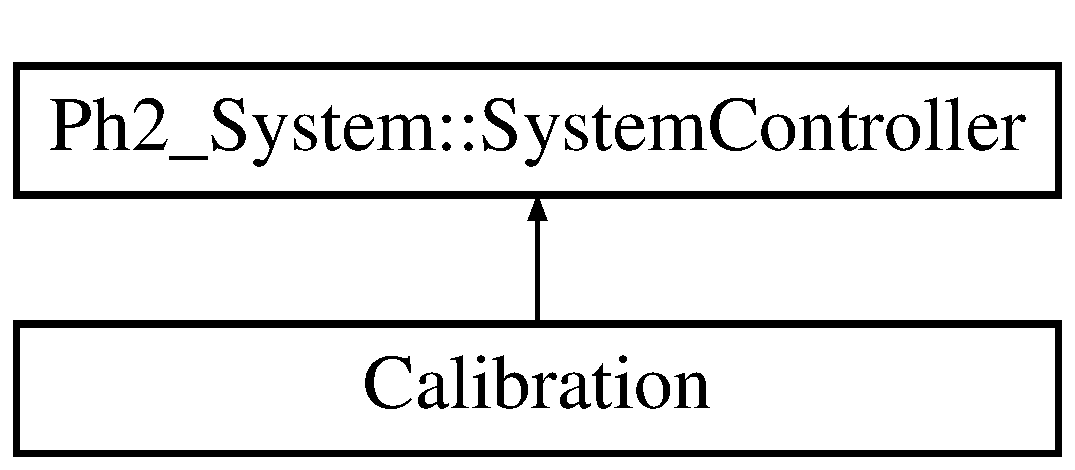
\includegraphics[height=2cm]{class_calibration}
\end{center}
\end{figure}
\subsection*{Public Member Functions}
\begin{CompactItemize}
\item 
\hyperlink{class_calibration_80f51a5ff7ec0f44d5388c9a61d1f20b}{Calibration} ()
\item 
\hyperlink{class_calibration_108efb6ccd8c98e5cac950be4bf0ac26}{$\sim$Calibration} ()
\item 
void \hyperlink{class_calibration_0d38b6198cd798ed2a2d3dceec93e6e1}{Initialise\-Test\-Group} ()
\item 
void \hyperlink{class_calibration_22a49d922a44c44eb1c5a7222c80e61a}{Vplus\-Scan} ()
\item 
void \hyperlink{class_calibration_90a0ab6faea40d474217ba5ab2c4d07f}{Offset\-Scan} ()
\item 
void \hyperlink{class_calibration_e154696d09e1b201ff1a28d99f2ed7a9}{Save\-Results} ()
\end{CompactItemize}
\subsection*{Private Member Functions}
\begin{CompactItemize}
\item 
void \hyperlink{class_calibration_6fbe71051d2006b42b0ef359bf5df44c}{Construct\-Test\-Group} (uint8\_\-t p\-Shelve\-Id, uint8\_\-t p\-Be\-Id, uint8\_\-t p\-Fe\-Id, uint8\_\-t p\-Cbc\-Id)
\item 
void \hyperlink{class_calibration_bb8c03c4daadb9063e4ef00303eda3bd}{Fit\-Vplus\-Vcth} (\hyperlink{class_ph2___hw_description_1_1_be_board}{Be\-Board} \&p\-Board, uint8\_\-t p\-Target\-Vcth, bool p\-Do\-Draw)
\item 
void \hyperlink{class_calibration_f70b5ced67623bace3f122e6ff96fe33}{set\-Global\-Reg} (\hyperlink{class_ph2___hw_description_1_1_be_board}{Be\-Board} \&p\-Board, std::string p\-Reg\-Name, uint8\_\-t p\-Reg\-Value)
\item 
void \hyperlink{class_calibration_4bcd5273c929942732583cf3b7b4fed8}{initialize\-SCurves} (\hyperlink{class_ph2___hw_description_1_1_be_board}{Be\-Board} \&p\-Board, uint8\_\-t p\-Group\-Id, uint8\_\-t p\-Value, TString p\-Parameter)
\item 
void \hyperlink{class_calibration_b4219c9939ddc49ca79fdaf9e13ba321}{measure\-SCurves} (\hyperlink{class_ph2___hw_description_1_1_be_board}{Be\-Board} \&p\-Board, uint8\_\-t p\-Group\-Id, uint32\_\-t p\-Eventsper\-Vcth, uint32\_\-t p\-Total\-Channels, bool p\-Hole\-Mode)
\item 
void \hyperlink{class_calibration_0c4e31e30ac0adf287e163960d761091}{process\-SCurves} (\hyperlink{class_ph2___hw_description_1_1_be_board}{Be\-Board} \&p\-Board, uint8\_\-t p\-Group\-Id, uint32\_\-t p\-Eventsper\-Vcth, uint8\_\-t p\-Value, TString p\-Parameter, bool p\-Hole\-Mode, bool p\-Do\-Draw)
\item 
uint32\_\-t \hyperlink{class_calibration_e8231544cb5098450e714f98a9e66a60}{fill\-Scurve\-Hists} (\hyperlink{class_ph2___hw_description_1_1_be_board}{Be\-Board} \&p\-Board, uint8\_\-t p\-Group\-Id, uint8\_\-t p\-Vcth, const \hyperlink{class_ph2___hw_interface_1_1_event}{Event} $\ast$p\-Event)
\item 
uint32\_\-t \hyperlink{class_calibration_cc42b29fa0301ecab251a51902603765}{Toggle\-Test\-Group} (\hyperlink{class_ph2___hw_description_1_1_be_board}{Be\-Board} \&p\-Board, uint8\_\-t p\-Group\-Id, bool p\-Hole\-Mode, bool p\-Enable)
\item 
uint32\_\-t \hyperlink{class_calibration_e61d5cd4dfc7b3725ee2f5d734860627}{Set\-Offset\-Target\-Bit\-Test\-Group} (\hyperlink{class_ph2___hw_description_1_1_be_board}{Be\-Board} \&p\-Board, uint8\_\-t p\-Group\-Id, bool p\-Hole\-Mode, uint8\_\-t p\-Target\-Bit, uint8\_\-t p\-Target\-Vcth)
\item 
void \hyperlink{class_calibration_29f921b720db68af7b1a889263aaac2a}{process\-SCurves\-Offset} (\hyperlink{class_ph2___hw_description_1_1_be_board}{Be\-Board} \&p\-Board, uint8\_\-t p\-Group\-Id, uint32\_\-t p\-Eventsper\-Vcth, uint8\_\-t p\-Target\-Vcth, uint8\_\-t p\-Target\-Bit, TString p\-Parameter, bool p\-Hole\-Mode, bool p\-Do\-Draw)
\item 
void \hyperlink{class_calibration_e68b10877c53dc83483e90391ce4b9ac}{Update\-Cbc\-Object} (\hyperlink{class_ph2___hw_description_1_1_be_board}{Be\-Board} \&p\-Board, uint8\_\-t p\-Group\-Id)
\end{CompactItemize}
\subsection*{Private Attributes}
\begin{CompactItemize}
\item 
\hyperlink{_channel_8h_1fc681fc13cd077738e86a5fbc1104d4}{Test\-Group\-Map} \hyperlink{class_calibration_c79d5ebc2766ebc9c5faf384a05581b0}{f\-Test\-Group\-Map}
\item 
\hyperlink{_channel_8h_1be8cf31d2544b84debee2220beeb318}{Test\-Group\-Graph\-Map} \hyperlink{class_calibration_7598aa1e8dab58e452923e54909f8a8e}{f\-Test\-Group\-Graph\-Map}
\item 
std::vector$<$ uint8\_\-t $>$ \hyperlink{class_calibration_d6fedaf43e799f69b7fd46d9347cc536}{f\-Vplus\-Values}
\item 
std::map$<$ \hyperlink{class_ph2___hw_description_1_1_cbc}{Cbc} $\ast$, TCanvas $\ast$ $>$ \hyperlink{class_calibration_e47a517af22b6c01652d8f5d5bd3ae20}{f\-Cbc\-Canvas\-Map}
\end{CompactItemize}


\subsection{Detailed Description}
Read/Write Cbc's registers on a file. 



\subsection{Constructor \& Destructor Documentation}
\hypertarget{class_calibration_80f51a5ff7ec0f44d5388c9a61d1f20b}{
\index{Calibration@{Calibration}!Calibration@{Calibration}}
\index{Calibration@{Calibration}!Calibration@{Calibration}}
\subsubsection[Calibration]{\setlength{\rightskip}{0pt plus 5cm}Calibration::Calibration ()}}
\label{class_calibration_80f51a5ff7ec0f44d5388c9a61d1f20b}


\hypertarget{class_calibration_108efb6ccd8c98e5cac950be4bf0ac26}{
\index{Calibration@{Calibration}!~Calibration@{$\sim$Calibration}}
\index{~Calibration@{$\sim$Calibration}!Calibration@{Calibration}}
\subsubsection[$\sim$Calibration]{\setlength{\rightskip}{0pt plus 5cm}Calibration::$\sim$Calibration ()}}
\label{class_calibration_108efb6ccd8c98e5cac950be4bf0ac26}




\subsection{Member Function Documentation}
\hypertarget{class_calibration_6fbe71051d2006b42b0ef359bf5df44c}{
\index{Calibration@{Calibration}!ConstructTestGroup@{ConstructTestGroup}}
\index{ConstructTestGroup@{ConstructTestGroup}!Calibration@{Calibration}}
\subsubsection[ConstructTestGroup]{\setlength{\rightskip}{0pt plus 5cm}void Calibration::Construct\-Test\-Group (uint8\_\-t {\em p\-Shelve\-Id}, uint8\_\-t {\em p\-Be\-Id}, uint8\_\-t {\em p\-Fe\-Id}, uint8\_\-t {\em p\-Cbc\-Id})\hspace{0.3cm}{\tt  \mbox{[}private\mbox{]}}}}
\label{class_calibration_6fbe71051d2006b42b0ef359bf5df44c}


\hypertarget{class_calibration_e8231544cb5098450e714f98a9e66a60}{
\index{Calibration@{Calibration}!fillScurveHists@{fillScurveHists}}
\index{fillScurveHists@{fillScurveHists}!Calibration@{Calibration}}
\subsubsection[fillScurveHists]{\setlength{\rightskip}{0pt plus 5cm}uint32\_\-t Calibration::fill\-Scurve\-Hists (\hyperlink{class_ph2___hw_description_1_1_be_board}{Be\-Board} \& {\em p\-Board}, uint8\_\-t {\em p\-Group\-Id}, uint8\_\-t {\em p\-Vcth}, const \hyperlink{class_ph2___hw_interface_1_1_event}{Event} $\ast$ {\em p\-Event})\hspace{0.3cm}{\tt  \mbox{[}private\mbox{]}}}}
\label{class_calibration_e8231544cb5098450e714f98a9e66a60}


\hypertarget{class_calibration_bb8c03c4daadb9063e4ef00303eda3bd}{
\index{Calibration@{Calibration}!FitVplusVcth@{FitVplusVcth}}
\index{FitVplusVcth@{FitVplusVcth}!Calibration@{Calibration}}
\subsubsection[FitVplusVcth]{\setlength{\rightskip}{0pt plus 5cm}void Calibration::Fit\-Vplus\-Vcth (\hyperlink{class_ph2___hw_description_1_1_be_board}{Be\-Board} \& {\em p\-Board}, uint8\_\-t {\em p\-Target\-Vcth}, bool {\em p\-Do\-Draw})\hspace{0.3cm}{\tt  \mbox{[}private\mbox{]}}}}
\label{class_calibration_bb8c03c4daadb9063e4ef00303eda3bd}


\hypertarget{class_calibration_0d38b6198cd798ed2a2d3dceec93e6e1}{
\index{Calibration@{Calibration}!InitialiseTestGroup@{InitialiseTestGroup}}
\index{InitialiseTestGroup@{InitialiseTestGroup}!Calibration@{Calibration}}
\subsubsection[InitialiseTestGroup]{\setlength{\rightskip}{0pt plus 5cm}void Calibration::Initialise\-Test\-Group ()}}
\label{class_calibration_0d38b6198cd798ed2a2d3dceec93e6e1}


\hypertarget{class_calibration_4bcd5273c929942732583cf3b7b4fed8}{
\index{Calibration@{Calibration}!initializeSCurves@{initializeSCurves}}
\index{initializeSCurves@{initializeSCurves}!Calibration@{Calibration}}
\subsubsection[initializeSCurves]{\setlength{\rightskip}{0pt plus 5cm}void Calibration::initialize\-SCurves (\hyperlink{class_ph2___hw_description_1_1_be_board}{Be\-Board} \& {\em p\-Board}, uint8\_\-t {\em p\-Group\-Id}, uint8\_\-t {\em p\-Value}, TString {\em p\-Parameter})\hspace{0.3cm}{\tt  \mbox{[}private\mbox{]}}}}
\label{class_calibration_4bcd5273c929942732583cf3b7b4fed8}


\hypertarget{class_calibration_b4219c9939ddc49ca79fdaf9e13ba321}{
\index{Calibration@{Calibration}!measureSCurves@{measureSCurves}}
\index{measureSCurves@{measureSCurves}!Calibration@{Calibration}}
\subsubsection[measureSCurves]{\setlength{\rightskip}{0pt plus 5cm}void Calibration::measure\-SCurves (\hyperlink{class_ph2___hw_description_1_1_be_board}{Be\-Board} \& {\em p\-Board}, uint8\_\-t {\em p\-Group\-Id}, uint32\_\-t {\em p\-Eventsper\-Vcth}, uint32\_\-t {\em p\-Total\-Channels}, bool {\em p\-Hole\-Mode})\hspace{0.3cm}{\tt  \mbox{[}private\mbox{]}}}}
\label{class_calibration_b4219c9939ddc49ca79fdaf9e13ba321}


\hypertarget{class_calibration_90a0ab6faea40d474217ba5ab2c4d07f}{
\index{Calibration@{Calibration}!OffsetScan@{OffsetScan}}
\index{OffsetScan@{OffsetScan}!Calibration@{Calibration}}
\subsubsection[OffsetScan]{\setlength{\rightskip}{0pt plus 5cm}void Calibration::Offset\-Scan ()}}
\label{class_calibration_90a0ab6faea40d474217ba5ab2c4d07f}


\hypertarget{class_calibration_0c4e31e30ac0adf287e163960d761091}{
\index{Calibration@{Calibration}!processSCurves@{processSCurves}}
\index{processSCurves@{processSCurves}!Calibration@{Calibration}}
\subsubsection[processSCurves]{\setlength{\rightskip}{0pt plus 5cm}void Calibration::process\-SCurves (\hyperlink{class_ph2___hw_description_1_1_be_board}{Be\-Board} \& {\em p\-Board}, uint8\_\-t {\em p\-Group\-Id}, uint32\_\-t {\em p\-Eventsper\-Vcth}, uint8\_\-t {\em p\-Value}, TString {\em p\-Parameter}, bool {\em p\-Hole\-Mode}, bool {\em p\-Do\-Draw})\hspace{0.3cm}{\tt  \mbox{[}private\mbox{]}}}}
\label{class_calibration_0c4e31e30ac0adf287e163960d761091}


\hypertarget{class_calibration_29f921b720db68af7b1a889263aaac2a}{
\index{Calibration@{Calibration}!processSCurvesOffset@{processSCurvesOffset}}
\index{processSCurvesOffset@{processSCurvesOffset}!Calibration@{Calibration}}
\subsubsection[processSCurvesOffset]{\setlength{\rightskip}{0pt plus 5cm}void Calibration::process\-SCurves\-Offset (\hyperlink{class_ph2___hw_description_1_1_be_board}{Be\-Board} \& {\em p\-Board}, uint8\_\-t {\em p\-Group\-Id}, uint32\_\-t {\em p\-Eventsper\-Vcth}, uint8\_\-t {\em p\-Target\-Vcth}, uint8\_\-t {\em p\-Target\-Bit}, TString {\em p\-Parameter}, bool {\em p\-Hole\-Mode}, bool {\em p\-Do\-Draw})\hspace{0.3cm}{\tt  \mbox{[}private\mbox{]}}}}
\label{class_calibration_29f921b720db68af7b1a889263aaac2a}


\hypertarget{class_calibration_e154696d09e1b201ff1a28d99f2ed7a9}{
\index{Calibration@{Calibration}!SaveResults@{SaveResults}}
\index{SaveResults@{SaveResults}!Calibration@{Calibration}}
\subsubsection[SaveResults]{\setlength{\rightskip}{0pt plus 5cm}void Calibration::Save\-Results ()}}
\label{class_calibration_e154696d09e1b201ff1a28d99f2ed7a9}


\hypertarget{class_calibration_f70b5ced67623bace3f122e6ff96fe33}{
\index{Calibration@{Calibration}!setGlobalReg@{setGlobalReg}}
\index{setGlobalReg@{setGlobalReg}!Calibration@{Calibration}}
\subsubsection[setGlobalReg]{\setlength{\rightskip}{0pt plus 5cm}void Calibration::set\-Global\-Reg (\hyperlink{class_ph2___hw_description_1_1_be_board}{Be\-Board} \& {\em p\-Board}, std::string {\em p\-Reg\-Name}, uint8\_\-t {\em p\-Reg\-Value})\hspace{0.3cm}{\tt  \mbox{[}private\mbox{]}}}}
\label{class_calibration_f70b5ced67623bace3f122e6ff96fe33}


\hypertarget{class_calibration_e61d5cd4dfc7b3725ee2f5d734860627}{
\index{Calibration@{Calibration}!SetOffsetTargetBitTestGroup@{SetOffsetTargetBitTestGroup}}
\index{SetOffsetTargetBitTestGroup@{SetOffsetTargetBitTestGroup}!Calibration@{Calibration}}
\subsubsection[SetOffsetTargetBitTestGroup]{\setlength{\rightskip}{0pt plus 5cm}uint32\_\-t Calibration::Set\-Offset\-Target\-Bit\-Test\-Group (\hyperlink{class_ph2___hw_description_1_1_be_board}{Be\-Board} \& {\em p\-Board}, uint8\_\-t {\em p\-Group\-Id}, bool {\em p\-Hole\-Mode}, uint8\_\-t {\em p\-Target\-Bit}, uint8\_\-t {\em p\-Target\-Vcth})\hspace{0.3cm}{\tt  \mbox{[}private\mbox{]}}}}
\label{class_calibration_e61d5cd4dfc7b3725ee2f5d734860627}


\hypertarget{class_calibration_cc42b29fa0301ecab251a51902603765}{
\index{Calibration@{Calibration}!ToggleTestGroup@{ToggleTestGroup}}
\index{ToggleTestGroup@{ToggleTestGroup}!Calibration@{Calibration}}
\subsubsection[ToggleTestGroup]{\setlength{\rightskip}{0pt plus 5cm}uint32\_\-t Calibration::Toggle\-Test\-Group (\hyperlink{class_ph2___hw_description_1_1_be_board}{Be\-Board} \& {\em p\-Board}, uint8\_\-t {\em p\-Group\-Id}, bool {\em p\-Hole\-Mode}, bool {\em p\-Enable})\hspace{0.3cm}{\tt  \mbox{[}private\mbox{]}}}}
\label{class_calibration_cc42b29fa0301ecab251a51902603765}


\hypertarget{class_calibration_e68b10877c53dc83483e90391ce4b9ac}{
\index{Calibration@{Calibration}!UpdateCbcObject@{UpdateCbcObject}}
\index{UpdateCbcObject@{UpdateCbcObject}!Calibration@{Calibration}}
\subsubsection[UpdateCbcObject]{\setlength{\rightskip}{0pt plus 5cm}void Calibration::Update\-Cbc\-Object (\hyperlink{class_ph2___hw_description_1_1_be_board}{Be\-Board} \& {\em p\-Board}, uint8\_\-t {\em p\-Group\-Id})\hspace{0.3cm}{\tt  \mbox{[}private\mbox{]}}}}
\label{class_calibration_e68b10877c53dc83483e90391ce4b9ac}


\hypertarget{class_calibration_22a49d922a44c44eb1c5a7222c80e61a}{
\index{Calibration@{Calibration}!VplusScan@{VplusScan}}
\index{VplusScan@{VplusScan}!Calibration@{Calibration}}
\subsubsection[VplusScan]{\setlength{\rightskip}{0pt plus 5cm}void Calibration::Vplus\-Scan ()}}
\label{class_calibration_22a49d922a44c44eb1c5a7222c80e61a}




\subsection{Field Documentation}
\hypertarget{class_calibration_e47a517af22b6c01652d8f5d5bd3ae20}{
\index{Calibration@{Calibration}!fCbcCanvasMap@{fCbcCanvasMap}}
\index{fCbcCanvasMap@{fCbcCanvasMap}!Calibration@{Calibration}}
\subsubsection[fCbcCanvasMap]{\setlength{\rightskip}{0pt plus 5cm}std::map$<$\hyperlink{class_ph2___hw_description_1_1_cbc}{Cbc}$\ast$, TCanvas$\ast$$>$ \hyperlink{class_calibration_e47a517af22b6c01652d8f5d5bd3ae20}{Calibration::f\-Cbc\-Canvas\-Map}\hspace{0.3cm}{\tt  \mbox{[}private\mbox{]}}}}
\label{class_calibration_e47a517af22b6c01652d8f5d5bd3ae20}


\hypertarget{class_calibration_7598aa1e8dab58e452923e54909f8a8e}{
\index{Calibration@{Calibration}!fTestGroupGraphMap@{fTestGroupGraphMap}}
\index{fTestGroupGraphMap@{fTestGroupGraphMap}!Calibration@{Calibration}}
\subsubsection[fTestGroupGraphMap]{\setlength{\rightskip}{0pt plus 5cm}\hyperlink{_channel_8h_1be8cf31d2544b84debee2220beeb318}{Test\-Group\-Graph\-Map} \hyperlink{class_calibration_7598aa1e8dab58e452923e54909f8a8e}{Calibration::f\-Test\-Group\-Graph\-Map}\hspace{0.3cm}{\tt  \mbox{[}private\mbox{]}}}}
\label{class_calibration_7598aa1e8dab58e452923e54909f8a8e}


\hypertarget{class_calibration_c79d5ebc2766ebc9c5faf384a05581b0}{
\index{Calibration@{Calibration}!fTestGroupMap@{fTestGroupMap}}
\index{fTestGroupMap@{fTestGroupMap}!Calibration@{Calibration}}
\subsubsection[fTestGroupMap]{\setlength{\rightskip}{0pt plus 5cm}\hyperlink{_channel_8h_1fc681fc13cd077738e86a5fbc1104d4}{Test\-Group\-Map} \hyperlink{class_calibration_c79d5ebc2766ebc9c5faf384a05581b0}{Calibration::f\-Test\-Group\-Map}\hspace{0.3cm}{\tt  \mbox{[}private\mbox{]}}}}
\label{class_calibration_c79d5ebc2766ebc9c5faf384a05581b0}


\hypertarget{class_calibration_d6fedaf43e799f69b7fd46d9347cc536}{
\index{Calibration@{Calibration}!fVplusValues@{fVplusValues}}
\index{fVplusValues@{fVplusValues}!Calibration@{Calibration}}
\subsubsection[fVplusValues]{\setlength{\rightskip}{0pt plus 5cm}std::vector$<$uint8\_\-t$>$ \hyperlink{class_calibration_d6fedaf43e799f69b7fd46d9347cc536}{Calibration::f\-Vplus\-Values}\hspace{0.3cm}{\tt  \mbox{[}private\mbox{]}}}}
\label{class_calibration_d6fedaf43e799f69b7fd46d9347cc536}




The documentation for this class was generated from the following files:\begin{CompactItemize}
\item 
tools/\hyperlink{_calibration_8h}{Calibration.h}\item 
tools/\hyperlink{_calibration_8cc}{Calibration.cc}\end{CompactItemize}

\hypertarget{class_ph2___hw_description_1_1_cbc}{\section{Ph2\-\_\-\-Hw\-Description\-:\-:Cbc Class Reference}
\label{class_ph2___hw_description_1_1_cbc}\index{Ph2\-\_\-\-Hw\-Description\-::\-Cbc@{Ph2\-\_\-\-Hw\-Description\-::\-Cbc}}
}


Read/\-Write \hyperlink{class_ph2___hw_description_1_1_cbc}{Cbc}'s registers on a file.  




{\ttfamily \#include $<$Cbc.\-h$>$}

Inheritance diagram for Ph2\-\_\-\-Hw\-Description\-:\-:Cbc\-:\begin{figure}[H]
\begin{center}
\leavevmode
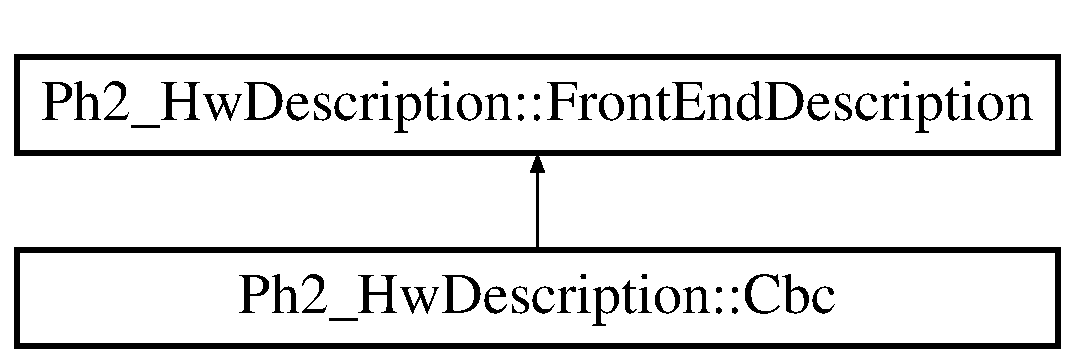
\includegraphics[height=2.000000cm]{class_ph2___hw_description_1_1_cbc}
\end{center}
\end{figure}
\subsection*{Public Member Functions}
\begin{DoxyCompactItemize}
\item 
\hyperlink{class_ph2___hw_description_1_1_cbc_a4569a0838d600c2d96f25adb6403e610}{Cbc} (\hyperlink{class_ph2___hw_description_1_1_f_e_description}{F\-E\-Description} \&p\-Fe\-Desc, uint8\-\_\-t p\-Cbc\-Id, std\-::string filename)
\item 
\hyperlink{class_ph2___hw_description_1_1_cbc_a8ad3757886613841f563b6eecd5d8406}{Cbc} (\hyperlink{class_ph2___hw_description_1_1_f_e_description}{F\-E\-Description} \&p\-Fe\-Desc, uint8\-\_\-t p\-Cbc\-Id, uint8\-\_\-t p\-Trigger\-Latency, uint8\-\_\-t p\-Vcth)
\item 
\hyperlink{class_ph2___hw_description_1_1_cbc_ad14c3944426f98d07914d0cb0fd38948}{Cbc} (\hyperlink{class_ph2___hw_description_1_1_f_e_description}{F\-E\-Description} \&p\-Fe\-Desc, uint8\-\_\-t p\-Cbc\-Id)
\item 
\hyperlink{class_ph2___hw_description_1_1_cbc_ad2ec420b5bd8e361a151b585a62c0ebe}{Cbc} (uint8\-\_\-t p\-Shelve\-Id, uint8\-\_\-t p\-Be\-Id, uint8\-\_\-t p\-F\-M\-C\-Id, uint8\-\_\-t p\-Fe\-Id, uint8\-\_\-t p\-Cbc\-Id, std\-::string filename)
\item 
\hyperlink{class_ph2___hw_description_1_1_cbc_a31698ad31b2484c74b87647e9451fc6d}{Cbc} (uint8\-\_\-t p\-Shelve\-Id, uint8\-\_\-t p\-Be\-Id, uint8\-\_\-t p\-F\-M\-C\-Id, uint8\-\_\-t p\-Fe\-Id, uint8\-\_\-t p\-Cbc\-Id, uint8\-\_\-t p\-Trigger\-Latency, uint8\-\_\-t p\-Vcth)
\item 
\hyperlink{class_ph2___hw_description_1_1_cbc_ac7e237f12e6950b45538e3706be11bb0}{Cbc} (uint8\-\_\-t p\-Shelve\-Id, uint8\-\_\-t p\-Be\-Id, uint8\-\_\-t p\-F\-M\-C\-Id, uint8\-\_\-t p\-Fe\-Id, uint8\-\_\-t p\-Cbc\-Id)
\item 
\hyperlink{class_ph2___hw_description_1_1_cbc_a5b7124456823871d611ada17ed0a51a1}{Cbc} ()
\item 
\hyperlink{class_ph2___hw_description_1_1_cbc_ab529cbb8cbbbc3b28a7ca2a472d4aa50}{Cbc} (const \hyperlink{class_ph2___hw_description_1_1_cbc}{Cbc} \&cbcobj)
\item 
\hyperlink{class_ph2___hw_description_1_1_cbc_a4e641d292073978e6e1b34fa91c13067}{$\sim$\-Cbc} ()
\item 
void \hyperlink{class_ph2___hw_description_1_1_cbc_afd6fdbe40eff3c160221a3a8acfb657d}{loadf\-Reg\-Map} (std\-::string filename)
\begin{DoxyCompactList}\small\item\em Load Reg\-Map from a file. \end{DoxyCompactList}\item 
uint8\-\_\-t \hyperlink{class_ph2___hw_description_1_1_cbc_a7dcee2bd6f0cbe1e9342f4d8e4229477}{get\-Trigger\-Latency} ()
\begin{DoxyCompactList}\small\item\em Get the register Trigger\-Latency from the Map. \end{DoxyCompactList}\item 
void \hyperlink{class_ph2___hw_description_1_1_cbc_af2ca8a515be91e594345f59765eedc86}{set\-Trigger\-Latency} (uint8\-\_\-t p\-Trigger\-Latency)
\begin{DoxyCompactList}\small\item\em Set the register Trigger\-Latency of the Map. \end{DoxyCompactList}\item 
uint8\-\_\-t \hyperlink{class_ph2___hw_description_1_1_cbc_ad52630f4caa9defc0c46e38c7f828d5f}{get\-Vcth} ()
\begin{DoxyCompactList}\small\item\em Get the register Vcth from the Map. \end{DoxyCompactList}\item 
void \hyperlink{class_ph2___hw_description_1_1_cbc_a055db371622ef5e565d7abd490d1b5bd}{set\-Vcth} (uint8\-\_\-t pset\-Vcth)
\begin{DoxyCompactList}\small\item\em Set the register Vcth of the Map. \end{DoxyCompactList}\item 
uint8\-\_\-t \hyperlink{class_ph2___hw_description_1_1_cbc_a8e29ea3bf86977585b3824941d948f91}{get\-Reg} (std\-::string p\-Reg)
\begin{DoxyCompactList}\small\item\em Get any register from the Map. \end{DoxyCompactList}\item 
void \hyperlink{class_ph2___hw_description_1_1_cbc_aa24292fe56d6b19ec08ba67f9790b5c7}{set\-Reg} (std\-::string p\-Reg, uint8\-\_\-t pset\-Value)
\begin{DoxyCompactList}\small\item\em Set any register of the Map. \end{DoxyCompactList}\item 
void \hyperlink{class_ph2___hw_description_1_1_cbc_a21a95937ae871d154b4d0f7f2fe6bd02}{write\-Reg\-Values} (std\-::string filename)
\begin{DoxyCompactList}\small\item\em Write the registers of the Map in a file. \end{DoxyCompactList}\item 
uint8\-\_\-t \hyperlink{class_ph2___hw_description_1_1_cbc_a14a78f27fb0e6c74622b6bc49259a2f3}{get\-Cbc\-Id} ()
\begin{DoxyCompactList}\small\item\em Get the \hyperlink{class_ph2___hw_description_1_1_cbc}{Cbc} Id. \end{DoxyCompactList}\item 
\hyperlink{namespace_ph2___hw_description_a9a23b373068f169aa67ca1d22c9a6001}{Cbc\-Reg\-Map} \hyperlink{class_ph2___hw_description_1_1_cbc_ad2bae647b2474b4737d7f2ede5a73ed3}{get\-Reg\-Map} ()
\begin{DoxyCompactList}\small\item\em Get the Map of the registers. \end{DoxyCompactList}\end{DoxyCompactItemize}
\subsection*{Data Fields}
\begin{DoxyCompactItemize}
\item 
uint8\-\_\-t \hyperlink{class_ph2___hw_description_1_1_cbc_a99b392306d4cdb7ffa7f956fc553011c}{f\-Cbc\-Id}
\end{DoxyCompactItemize}
\subsection*{Protected Attributes}
\begin{DoxyCompactItemize}
\item 
\hyperlink{namespace_ph2___hw_description_a9a23b373068f169aa67ca1d22c9a6001}{Cbc\-Reg\-Map} \hyperlink{class_ph2___hw_description_1_1_cbc_ab4dbf1af172e821d95f77acb7e4fb962}{f\-Reg\-Map}
\end{DoxyCompactItemize}


\subsection{Detailed Description}
Read/\-Write \hyperlink{class_ph2___hw_description_1_1_cbc}{Cbc}'s registers on a file. 

\subsection{Constructor \& Destructor Documentation}
\hypertarget{class_ph2___hw_description_1_1_cbc_a4569a0838d600c2d96f25adb6403e610}{\index{Ph2\-\_\-\-Hw\-Description\-::\-Cbc@{Ph2\-\_\-\-Hw\-Description\-::\-Cbc}!Cbc@{Cbc}}
\index{Cbc@{Cbc}!Ph2_HwDescription::Cbc@{Ph2\-\_\-\-Hw\-Description\-::\-Cbc}}
\subsubsection[{Cbc}]{\setlength{\rightskip}{0pt plus 5cm}Ph2\-\_\-\-Hw\-Description\-::\-Cbc\-::\-Cbc (
\begin{DoxyParamCaption}
\item[{{\bf F\-E\-Description} \&}]{p\-Fe\-Desc, }
\item[{uint8\-\_\-t}]{p\-Cbc\-Id, }
\item[{std\-::string}]{filename}
\end{DoxyParamCaption}
)}}\label{class_ph2___hw_description_1_1_cbc_a4569a0838d600c2d96f25adb6403e610}
\hypertarget{class_ph2___hw_description_1_1_cbc_a8ad3757886613841f563b6eecd5d8406}{\index{Ph2\-\_\-\-Hw\-Description\-::\-Cbc@{Ph2\-\_\-\-Hw\-Description\-::\-Cbc}!Cbc@{Cbc}}
\index{Cbc@{Cbc}!Ph2_HwDescription::Cbc@{Ph2\-\_\-\-Hw\-Description\-::\-Cbc}}
\subsubsection[{Cbc}]{\setlength{\rightskip}{0pt plus 5cm}Ph2\-\_\-\-Hw\-Description\-::\-Cbc\-::\-Cbc (
\begin{DoxyParamCaption}
\item[{{\bf F\-E\-Description} \&}]{p\-Fe\-Desc, }
\item[{uint8\-\_\-t}]{p\-Cbc\-Id, }
\item[{uint8\-\_\-t}]{p\-Trigger\-Latency, }
\item[{uint8\-\_\-t}]{p\-Vcth}
\end{DoxyParamCaption}
)}}\label{class_ph2___hw_description_1_1_cbc_a8ad3757886613841f563b6eecd5d8406}
\hypertarget{class_ph2___hw_description_1_1_cbc_ad14c3944426f98d07914d0cb0fd38948}{\index{Ph2\-\_\-\-Hw\-Description\-::\-Cbc@{Ph2\-\_\-\-Hw\-Description\-::\-Cbc}!Cbc@{Cbc}}
\index{Cbc@{Cbc}!Ph2_HwDescription::Cbc@{Ph2\-\_\-\-Hw\-Description\-::\-Cbc}}
\subsubsection[{Cbc}]{\setlength{\rightskip}{0pt plus 5cm}Ph2\-\_\-\-Hw\-Description\-::\-Cbc\-::\-Cbc (
\begin{DoxyParamCaption}
\item[{{\bf F\-E\-Description} \&}]{p\-Fe\-Desc, }
\item[{uint8\-\_\-t}]{p\-Cbc\-Id}
\end{DoxyParamCaption}
)}}\label{class_ph2___hw_description_1_1_cbc_ad14c3944426f98d07914d0cb0fd38948}
\hypertarget{class_ph2___hw_description_1_1_cbc_ad2ec420b5bd8e361a151b585a62c0ebe}{\index{Ph2\-\_\-\-Hw\-Description\-::\-Cbc@{Ph2\-\_\-\-Hw\-Description\-::\-Cbc}!Cbc@{Cbc}}
\index{Cbc@{Cbc}!Ph2_HwDescription::Cbc@{Ph2\-\_\-\-Hw\-Description\-::\-Cbc}}
\subsubsection[{Cbc}]{\setlength{\rightskip}{0pt plus 5cm}Ph2\-\_\-\-Hw\-Description\-::\-Cbc\-::\-Cbc (
\begin{DoxyParamCaption}
\item[{uint8\-\_\-t}]{p\-Shelve\-Id, }
\item[{uint8\-\_\-t}]{p\-Be\-Id, }
\item[{uint8\-\_\-t}]{p\-F\-M\-C\-Id, }
\item[{uint8\-\_\-t}]{p\-Fe\-Id, }
\item[{uint8\-\_\-t}]{p\-Cbc\-Id, }
\item[{std\-::string}]{filename}
\end{DoxyParamCaption}
)}}\label{class_ph2___hw_description_1_1_cbc_ad2ec420b5bd8e361a151b585a62c0ebe}
\hypertarget{class_ph2___hw_description_1_1_cbc_a31698ad31b2484c74b87647e9451fc6d}{\index{Ph2\-\_\-\-Hw\-Description\-::\-Cbc@{Ph2\-\_\-\-Hw\-Description\-::\-Cbc}!Cbc@{Cbc}}
\index{Cbc@{Cbc}!Ph2_HwDescription::Cbc@{Ph2\-\_\-\-Hw\-Description\-::\-Cbc}}
\subsubsection[{Cbc}]{\setlength{\rightskip}{0pt plus 5cm}Ph2\-\_\-\-Hw\-Description\-::\-Cbc\-::\-Cbc (
\begin{DoxyParamCaption}
\item[{uint8\-\_\-t}]{p\-Shelve\-Id, }
\item[{uint8\-\_\-t}]{p\-Be\-Id, }
\item[{uint8\-\_\-t}]{p\-F\-M\-C\-Id, }
\item[{uint8\-\_\-t}]{p\-Fe\-Id, }
\item[{uint8\-\_\-t}]{p\-Cbc\-Id, }
\item[{uint8\-\_\-t}]{p\-Trigger\-Latency, }
\item[{uint8\-\_\-t}]{p\-Vcth}
\end{DoxyParamCaption}
)}}\label{class_ph2___hw_description_1_1_cbc_a31698ad31b2484c74b87647e9451fc6d}
\hypertarget{class_ph2___hw_description_1_1_cbc_ac7e237f12e6950b45538e3706be11bb0}{\index{Ph2\-\_\-\-Hw\-Description\-::\-Cbc@{Ph2\-\_\-\-Hw\-Description\-::\-Cbc}!Cbc@{Cbc}}
\index{Cbc@{Cbc}!Ph2_HwDescription::Cbc@{Ph2\-\_\-\-Hw\-Description\-::\-Cbc}}
\subsubsection[{Cbc}]{\setlength{\rightskip}{0pt plus 5cm}Ph2\-\_\-\-Hw\-Description\-::\-Cbc\-::\-Cbc (
\begin{DoxyParamCaption}
\item[{uint8\-\_\-t}]{p\-Shelve\-Id, }
\item[{uint8\-\_\-t}]{p\-Be\-Id, }
\item[{uint8\-\_\-t}]{p\-F\-M\-C\-Id, }
\item[{uint8\-\_\-t}]{p\-Fe\-Id, }
\item[{uint8\-\_\-t}]{p\-Cbc\-Id}
\end{DoxyParamCaption}
)}}\label{class_ph2___hw_description_1_1_cbc_ac7e237f12e6950b45538e3706be11bb0}
\hypertarget{class_ph2___hw_description_1_1_cbc_a5b7124456823871d611ada17ed0a51a1}{\index{Ph2\-\_\-\-Hw\-Description\-::\-Cbc@{Ph2\-\_\-\-Hw\-Description\-::\-Cbc}!Cbc@{Cbc}}
\index{Cbc@{Cbc}!Ph2_HwDescription::Cbc@{Ph2\-\_\-\-Hw\-Description\-::\-Cbc}}
\subsubsection[{Cbc}]{\setlength{\rightskip}{0pt plus 5cm}Ph2\-\_\-\-Hw\-Description\-::\-Cbc\-::\-Cbc (
\begin{DoxyParamCaption}
{}
\end{DoxyParamCaption}
)}}\label{class_ph2___hw_description_1_1_cbc_a5b7124456823871d611ada17ed0a51a1}
\hypertarget{class_ph2___hw_description_1_1_cbc_ab529cbb8cbbbc3b28a7ca2a472d4aa50}{\index{Ph2\-\_\-\-Hw\-Description\-::\-Cbc@{Ph2\-\_\-\-Hw\-Description\-::\-Cbc}!Cbc@{Cbc}}
\index{Cbc@{Cbc}!Ph2_HwDescription::Cbc@{Ph2\-\_\-\-Hw\-Description\-::\-Cbc}}
\subsubsection[{Cbc}]{\setlength{\rightskip}{0pt plus 5cm}Ph2\-\_\-\-Hw\-Description\-::\-Cbc\-::\-Cbc (
\begin{DoxyParamCaption}
\item[{const {\bf Cbc} \&}]{cbcobj}
\end{DoxyParamCaption}
)}}\label{class_ph2___hw_description_1_1_cbc_ab529cbb8cbbbc3b28a7ca2a472d4aa50}
\hypertarget{class_ph2___hw_description_1_1_cbc_a4e641d292073978e6e1b34fa91c13067}{\index{Ph2\-\_\-\-Hw\-Description\-::\-Cbc@{Ph2\-\_\-\-Hw\-Description\-::\-Cbc}!$\sim$\-Cbc@{$\sim$\-Cbc}}
\index{$\sim$\-Cbc@{$\sim$\-Cbc}!Ph2_HwDescription::Cbc@{Ph2\-\_\-\-Hw\-Description\-::\-Cbc}}
\subsubsection[{$\sim$\-Cbc}]{\setlength{\rightskip}{0pt plus 5cm}Ph2\-\_\-\-Hw\-Description\-::\-Cbc\-::$\sim$\-Cbc (
\begin{DoxyParamCaption}
{}
\end{DoxyParamCaption}
)}}\label{class_ph2___hw_description_1_1_cbc_a4e641d292073978e6e1b34fa91c13067}


\subsection{Member Function Documentation}
\hypertarget{class_ph2___hw_description_1_1_cbc_a14a78f27fb0e6c74622b6bc49259a2f3}{\index{Ph2\-\_\-\-Hw\-Description\-::\-Cbc@{Ph2\-\_\-\-Hw\-Description\-::\-Cbc}!get\-Cbc\-Id@{get\-Cbc\-Id}}
\index{get\-Cbc\-Id@{get\-Cbc\-Id}!Ph2_HwDescription::Cbc@{Ph2\-\_\-\-Hw\-Description\-::\-Cbc}}
\subsubsection[{get\-Cbc\-Id}]{\setlength{\rightskip}{0pt plus 5cm}uint8\-\_\-t Ph2\-\_\-\-Hw\-Description\-::\-Cbc\-::get\-Cbc\-Id (
\begin{DoxyParamCaption}
{}
\end{DoxyParamCaption}
)\hspace{0.3cm}{\ttfamily [inline]}}}\label{class_ph2___hw_description_1_1_cbc_a14a78f27fb0e6c74622b6bc49259a2f3}


Get the \hyperlink{class_ph2___hw_description_1_1_cbc}{Cbc} Id. 

\begin{DoxyReturn}{Returns}
The \hyperlink{class_ph2___hw_description_1_1_cbc}{Cbc} I\-D 
\end{DoxyReturn}
\hypertarget{class_ph2___hw_description_1_1_cbc_a8e29ea3bf86977585b3824941d948f91}{\index{Ph2\-\_\-\-Hw\-Description\-::\-Cbc@{Ph2\-\_\-\-Hw\-Description\-::\-Cbc}!get\-Reg@{get\-Reg}}
\index{get\-Reg@{get\-Reg}!Ph2_HwDescription::Cbc@{Ph2\-\_\-\-Hw\-Description\-::\-Cbc}}
\subsubsection[{get\-Reg}]{\setlength{\rightskip}{0pt plus 5cm}uint8\-\_\-t Ph2\-\_\-\-Hw\-Description\-::\-Cbc\-::get\-Reg (
\begin{DoxyParamCaption}
\item[{std\-::string}]{p\-Reg}
\end{DoxyParamCaption}
)}}\label{class_ph2___hw_description_1_1_cbc_a8e29ea3bf86977585b3824941d948f91}


Get any register from the Map. 


\begin{DoxyParams}{Parameters}
{\em p\-Reg} & \\
\hline
\end{DoxyParams}
\begin{DoxyReturn}{Returns}
The value of the register 
\end{DoxyReturn}
\hypertarget{class_ph2___hw_description_1_1_cbc_ad2bae647b2474b4737d7f2ede5a73ed3}{\index{Ph2\-\_\-\-Hw\-Description\-::\-Cbc@{Ph2\-\_\-\-Hw\-Description\-::\-Cbc}!get\-Reg\-Map@{get\-Reg\-Map}}
\index{get\-Reg\-Map@{get\-Reg\-Map}!Ph2_HwDescription::Cbc@{Ph2\-\_\-\-Hw\-Description\-::\-Cbc}}
\subsubsection[{get\-Reg\-Map}]{\setlength{\rightskip}{0pt plus 5cm}{\bf Cbc\-Reg\-Map} Ph2\-\_\-\-Hw\-Description\-::\-Cbc\-::get\-Reg\-Map (
\begin{DoxyParamCaption}
{}
\end{DoxyParamCaption}
)\hspace{0.3cm}{\ttfamily [inline]}}}\label{class_ph2___hw_description_1_1_cbc_ad2bae647b2474b4737d7f2ede5a73ed3}


Get the Map of the registers. 

\begin{DoxyReturn}{Returns}
The map of register 
\end{DoxyReturn}
\hypertarget{class_ph2___hw_description_1_1_cbc_a7dcee2bd6f0cbe1e9342f4d8e4229477}{\index{Ph2\-\_\-\-Hw\-Description\-::\-Cbc@{Ph2\-\_\-\-Hw\-Description\-::\-Cbc}!get\-Trigger\-Latency@{get\-Trigger\-Latency}}
\index{get\-Trigger\-Latency@{get\-Trigger\-Latency}!Ph2_HwDescription::Cbc@{Ph2\-\_\-\-Hw\-Description\-::\-Cbc}}
\subsubsection[{get\-Trigger\-Latency}]{\setlength{\rightskip}{0pt plus 5cm}uint8\-\_\-t Ph2\-\_\-\-Hw\-Description\-::\-Cbc\-::get\-Trigger\-Latency (
\begin{DoxyParamCaption}
{}
\end{DoxyParamCaption}
)}}\label{class_ph2___hw_description_1_1_cbc_a7dcee2bd6f0cbe1e9342f4d8e4229477}


Get the register Trigger\-Latency from the Map. 

\begin{DoxyReturn}{Returns}
The value of Trigger\-Lantency 
\end{DoxyReturn}
\hypertarget{class_ph2___hw_description_1_1_cbc_ad52630f4caa9defc0c46e38c7f828d5f}{\index{Ph2\-\_\-\-Hw\-Description\-::\-Cbc@{Ph2\-\_\-\-Hw\-Description\-::\-Cbc}!get\-Vcth@{get\-Vcth}}
\index{get\-Vcth@{get\-Vcth}!Ph2_HwDescription::Cbc@{Ph2\-\_\-\-Hw\-Description\-::\-Cbc}}
\subsubsection[{get\-Vcth}]{\setlength{\rightskip}{0pt plus 5cm}uint8\-\_\-t Ph2\-\_\-\-Hw\-Description\-::\-Cbc\-::get\-Vcth (
\begin{DoxyParamCaption}
{}
\end{DoxyParamCaption}
)}}\label{class_ph2___hw_description_1_1_cbc_ad52630f4caa9defc0c46e38c7f828d5f}


Get the register Vcth from the Map. 

\begin{DoxyReturn}{Returns}
The value of Vcth 
\end{DoxyReturn}
\hypertarget{class_ph2___hw_description_1_1_cbc_afd6fdbe40eff3c160221a3a8acfb657d}{\index{Ph2\-\_\-\-Hw\-Description\-::\-Cbc@{Ph2\-\_\-\-Hw\-Description\-::\-Cbc}!loadf\-Reg\-Map@{loadf\-Reg\-Map}}
\index{loadf\-Reg\-Map@{loadf\-Reg\-Map}!Ph2_HwDescription::Cbc@{Ph2\-\_\-\-Hw\-Description\-::\-Cbc}}
\subsubsection[{loadf\-Reg\-Map}]{\setlength{\rightskip}{0pt plus 5cm}void Ph2\-\_\-\-Hw\-Description\-::\-Cbc\-::loadf\-Reg\-Map (
\begin{DoxyParamCaption}
\item[{std\-::string}]{filename}
\end{DoxyParamCaption}
)}}\label{class_ph2___hw_description_1_1_cbc_afd6fdbe40eff3c160221a3a8acfb657d}


Load Reg\-Map from a file. 


\begin{DoxyParams}{Parameters}
{\em filename} & \\
\hline
\end{DoxyParams}
\hypertarget{class_ph2___hw_description_1_1_cbc_aa24292fe56d6b19ec08ba67f9790b5c7}{\index{Ph2\-\_\-\-Hw\-Description\-::\-Cbc@{Ph2\-\_\-\-Hw\-Description\-::\-Cbc}!set\-Reg@{set\-Reg}}
\index{set\-Reg@{set\-Reg}!Ph2_HwDescription::Cbc@{Ph2\-\_\-\-Hw\-Description\-::\-Cbc}}
\subsubsection[{set\-Reg}]{\setlength{\rightskip}{0pt plus 5cm}void Ph2\-\_\-\-Hw\-Description\-::\-Cbc\-::set\-Reg (
\begin{DoxyParamCaption}
\item[{std\-::string}]{p\-Reg, }
\item[{uint8\-\_\-t}]{pset\-Value}
\end{DoxyParamCaption}
)}}\label{class_ph2___hw_description_1_1_cbc_aa24292fe56d6b19ec08ba67f9790b5c7}


Set any register of the Map. 


\begin{DoxyParams}{Parameters}
{\em p\-Reg} & \\
\hline
{\em pset\-Value} & \\
\hline
\end{DoxyParams}
\hypertarget{class_ph2___hw_description_1_1_cbc_af2ca8a515be91e594345f59765eedc86}{\index{Ph2\-\_\-\-Hw\-Description\-::\-Cbc@{Ph2\-\_\-\-Hw\-Description\-::\-Cbc}!set\-Trigger\-Latency@{set\-Trigger\-Latency}}
\index{set\-Trigger\-Latency@{set\-Trigger\-Latency}!Ph2_HwDescription::Cbc@{Ph2\-\_\-\-Hw\-Description\-::\-Cbc}}
\subsubsection[{set\-Trigger\-Latency}]{\setlength{\rightskip}{0pt plus 5cm}void Ph2\-\_\-\-Hw\-Description\-::\-Cbc\-::set\-Trigger\-Latency (
\begin{DoxyParamCaption}
\item[{uint8\-\_\-t}]{p\-Trigger\-Latency}
\end{DoxyParamCaption}
)}}\label{class_ph2___hw_description_1_1_cbc_af2ca8a515be91e594345f59765eedc86}


Set the register Trigger\-Latency of the Map. 


\begin{DoxyParams}{Parameters}
{\em p\-Trigger\-Latency} & \\
\hline
\end{DoxyParams}
\hypertarget{class_ph2___hw_description_1_1_cbc_a055db371622ef5e565d7abd490d1b5bd}{\index{Ph2\-\_\-\-Hw\-Description\-::\-Cbc@{Ph2\-\_\-\-Hw\-Description\-::\-Cbc}!set\-Vcth@{set\-Vcth}}
\index{set\-Vcth@{set\-Vcth}!Ph2_HwDescription::Cbc@{Ph2\-\_\-\-Hw\-Description\-::\-Cbc}}
\subsubsection[{set\-Vcth}]{\setlength{\rightskip}{0pt plus 5cm}void Ph2\-\_\-\-Hw\-Description\-::\-Cbc\-::set\-Vcth (
\begin{DoxyParamCaption}
\item[{uint8\-\_\-t}]{pset\-Vcth}
\end{DoxyParamCaption}
)}}\label{class_ph2___hw_description_1_1_cbc_a055db371622ef5e565d7abd490d1b5bd}


Set the register Vcth of the Map. 


\begin{DoxyParams}{Parameters}
{\em pset\-Vcth} & \\
\hline
\end{DoxyParams}
\hypertarget{class_ph2___hw_description_1_1_cbc_a21a95937ae871d154b4d0f7f2fe6bd02}{\index{Ph2\-\_\-\-Hw\-Description\-::\-Cbc@{Ph2\-\_\-\-Hw\-Description\-::\-Cbc}!write\-Reg\-Values@{write\-Reg\-Values}}
\index{write\-Reg\-Values@{write\-Reg\-Values}!Ph2_HwDescription::Cbc@{Ph2\-\_\-\-Hw\-Description\-::\-Cbc}}
\subsubsection[{write\-Reg\-Values}]{\setlength{\rightskip}{0pt plus 5cm}void Ph2\-\_\-\-Hw\-Description\-::\-Cbc\-::write\-Reg\-Values (
\begin{DoxyParamCaption}
\item[{std\-::string}]{filename}
\end{DoxyParamCaption}
)}}\label{class_ph2___hw_description_1_1_cbc_a21a95937ae871d154b4d0f7f2fe6bd02}


Write the registers of the Map in a file. 


\begin{DoxyParams}{Parameters}
{\em filename} & \\
\hline
\end{DoxyParams}


\subsection{Field Documentation}
\hypertarget{class_ph2___hw_description_1_1_cbc_a99b392306d4cdb7ffa7f956fc553011c}{\index{Ph2\-\_\-\-Hw\-Description\-::\-Cbc@{Ph2\-\_\-\-Hw\-Description\-::\-Cbc}!f\-Cbc\-Id@{f\-Cbc\-Id}}
\index{f\-Cbc\-Id@{f\-Cbc\-Id}!Ph2_HwDescription::Cbc@{Ph2\-\_\-\-Hw\-Description\-::\-Cbc}}
\subsubsection[{f\-Cbc\-Id}]{\setlength{\rightskip}{0pt plus 5cm}uint8\-\_\-t Ph2\-\_\-\-Hw\-Description\-::\-Cbc\-::f\-Cbc\-Id}}\label{class_ph2___hw_description_1_1_cbc_a99b392306d4cdb7ffa7f956fc553011c}
\hypertarget{class_ph2___hw_description_1_1_cbc_ab4dbf1af172e821d95f77acb7e4fb962}{\index{Ph2\-\_\-\-Hw\-Description\-::\-Cbc@{Ph2\-\_\-\-Hw\-Description\-::\-Cbc}!f\-Reg\-Map@{f\-Reg\-Map}}
\index{f\-Reg\-Map@{f\-Reg\-Map}!Ph2_HwDescription::Cbc@{Ph2\-\_\-\-Hw\-Description\-::\-Cbc}}
\subsubsection[{f\-Reg\-Map}]{\setlength{\rightskip}{0pt plus 5cm}{\bf Cbc\-Reg\-Map} Ph2\-\_\-\-Hw\-Description\-::\-Cbc\-::f\-Reg\-Map\hspace{0.3cm}{\ttfamily [protected]}}}\label{class_ph2___hw_description_1_1_cbc_ab4dbf1af172e821d95f77acb7e4fb962}


The documentation for this class was generated from the following files\-:\begin{DoxyCompactItemize}
\item 
H\-W\-Description/\hyperlink{_cbc_8h}{Cbc.\-h}\item 
H\-W\-Description/\hyperlink{_cbc_8cc}{Cbc.\-cc}\end{DoxyCompactItemize}

\hypertarget{struct_ph2___hw_description_1_1_cbc_comparer}{\section{Ph2\-\_\-\-Hw\-Description\-:\-:Cbc\-Comparer Struct Reference}
\label{struct_ph2___hw_description_1_1_cbc_comparer}\index{Ph2\-\_\-\-Hw\-Description\-::\-Cbc\-Comparer@{Ph2\-\_\-\-Hw\-Description\-::\-Cbc\-Comparer}}
}


Compare two \hyperlink{class_ph2___hw_description_1_1_cbc}{Cbc} by their I\-D.  




{\ttfamily \#include $<$Cbc.\-h$>$}

\subsection*{Public Member Functions}
\begin{DoxyCompactItemize}
\item 
bool \hyperlink{struct_ph2___hw_description_1_1_cbc_comparer_af83d2c46bcdcb36adcd0ae91f929942a}{operator()} (\hyperlink{class_ph2___hw_description_1_1_cbc}{Cbc} \&cbc1, \hyperlink{class_ph2___hw_description_1_1_cbc}{Cbc} \&cbc2)
\end{DoxyCompactItemize}


\subsection{Detailed Description}
Compare two \hyperlink{class_ph2___hw_description_1_1_cbc}{Cbc} by their I\-D. 

\subsection{Member Function Documentation}
\hypertarget{struct_ph2___hw_description_1_1_cbc_comparer_af83d2c46bcdcb36adcd0ae91f929942a}{\index{Ph2\-\_\-\-Hw\-Description\-::\-Cbc\-Comparer@{Ph2\-\_\-\-Hw\-Description\-::\-Cbc\-Comparer}!operator()@{operator()}}
\index{operator()@{operator()}!Ph2_HwDescription::CbcComparer@{Ph2\-\_\-\-Hw\-Description\-::\-Cbc\-Comparer}}
\subsubsection[{operator()}]{\setlength{\rightskip}{0pt plus 5cm}bool Ph2\-\_\-\-Hw\-Description\-::\-Cbc\-Comparer\-::operator() (
\begin{DoxyParamCaption}
\item[{{\bf Cbc} \&}]{cbc1, }
\item[{{\bf Cbc} \&}]{cbc2}
\end{DoxyParamCaption}
)}}\label{struct_ph2___hw_description_1_1_cbc_comparer_af83d2c46bcdcb36adcd0ae91f929942a}


The documentation for this struct was generated from the following files\-:\begin{DoxyCompactItemize}
\item 
H\-W\-Description/\hyperlink{_cbc_8h}{Cbc.\-h}\item 
H\-W\-Description/\hyperlink{_cbc_8cc}{Cbc.\-cc}\end{DoxyCompactItemize}

\hypertarget{class_ph2___hw_interface_1_1_cbc_interface}{\section{Ph2\-\_\-\-Hw\-Interface\-:\-:Cbc\-Interface Class Reference}
\label{class_ph2___hw_interface_1_1_cbc_interface}\index{Ph2\-\_\-\-Hw\-Interface\-::\-Cbc\-Interface@{Ph2\-\_\-\-Hw\-Interface\-::\-Cbc\-Interface}}
}
Inheritance diagram for Ph2\-\_\-\-Hw\-Interface\-:\-:Cbc\-Interface\-:\begin{figure}[H]
\begin{center}
\leavevmode
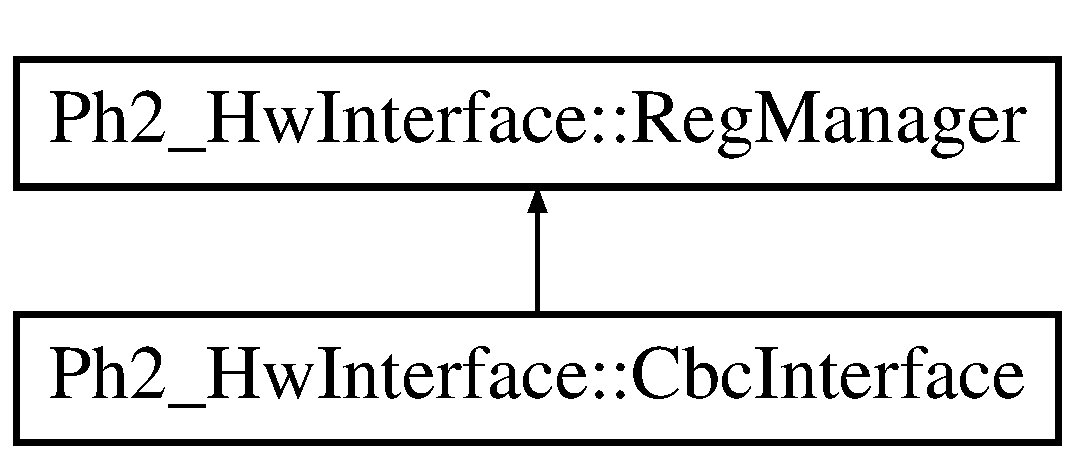
\includegraphics[height=2.000000cm]{class_ph2___hw_interface_1_1_cbc_interface}
\end{center}
\end{figure}
\subsection*{Public Member Functions}
\begin{DoxyCompactItemize}
\item 
\hypertarget{class_ph2___hw_interface_1_1_cbc_interface_a3ddefe5549da06a7d26fee1502a792b4}{{\bfseries Cbc\-Interface} (const char $\ast$pu\-Hal\-Config\-File\-Name)}\label{class_ph2___hw_interface_1_1_cbc_interface_a3ddefe5549da06a7d26fee1502a792b4}

\item 
\hypertarget{class_ph2___hw_interface_1_1_cbc_interface_af5cf4eb5b7134835f00349cb19f35c56}{void \hyperlink{class_ph2___hw_interface_1_1_cbc_interface_af5cf4eb5b7134835f00349cb19f35c56}{Configure\-Cbc} (Cbc \&p\-Cbc)}\label{class_ph2___hw_interface_1_1_cbc_interface_af5cf4eb5b7134835f00349cb19f35c56}

\begin{DoxyCompactList}\small\item\em Configure the Cbc after the Cbc\-Config\-File. \end{DoxyCompactList}\item 
\hypertarget{class_ph2___hw_interface_1_1_cbc_interface_a498d71b5709e0524b8e9dc50b92d1424}{void \hyperlink{class_ph2___hw_interface_1_1_cbc_interface_a498d71b5709e0524b8e9dc50b92d1424}{Update\-Cbc\-Write} (Cbc \&p\-Cbc, const std\-::string \&p\-Reg\-Node, uint32\-\_\-t \&p\-Word)}\label{class_ph2___hw_interface_1_1_cbc_interface_a498d71b5709e0524b8e9dc50b92d1424}

\begin{DoxyCompactList}\small\item\em Write the designated register in both Cbc and Cbc\-Config\-File. \end{DoxyCompactList}\item 
\hypertarget{class_ph2___hw_interface_1_1_cbc_interface_ab08ea1de98fe120098a4f5c52e017393}{void \hyperlink{class_ph2___hw_interface_1_1_cbc_interface_ab08ea1de98fe120098a4f5c52e017393}{Update\-Cbc\-Read} (Cbc \&p\-Cbc, const std\-::string \&p\-Reg\-Node)}\label{class_ph2___hw_interface_1_1_cbc_interface_ab08ea1de98fe120098a4f5c52e017393}

\begin{DoxyCompactList}\small\item\em Read the designated register in the Cbc and update the Cbc\-Config\-File. \end{DoxyCompactList}\end{DoxyCompactItemize}
\subsection*{Static Public Attributes}
\begin{DoxyCompactItemize}
\item 
\hypertarget{class_ph2___hw_interface_1_1_cbc_interface_ab45dcb5563c94075ac0a3e17d17c1fd4}{static const std\-::string {\bfseries f\-Str\-I2c\-Settings} = I2\-C\-\_\-\-S\-E\-T\-T\-I\-N\-G\-S}\label{class_ph2___hw_interface_1_1_cbc_interface_ab45dcb5563c94075ac0a3e17d17c1fd4}

\item 
\hypertarget{class_ph2___hw_interface_1_1_cbc_interface_a350e32baca2a50220eeff24b9fa07054}{static const std\-::string {\bfseries f\-Str\-I2c\-Command} = I2\-C\-\_\-\-C\-O\-M\-M\-A\-N\-D}\label{class_ph2___hw_interface_1_1_cbc_interface_a350e32baca2a50220eeff24b9fa07054}

\item 
\hypertarget{class_ph2___hw_interface_1_1_cbc_interface_a6a0730099e121a7707615ba6969afe80}{static const std\-::string {\bfseries f\-Str\-I2c\-Reply} = I2\-C\-\_\-\-R\-E\-P\-L\-Y}\label{class_ph2___hw_interface_1_1_cbc_interface_a6a0730099e121a7707615ba6969afe80}

\item 
\hypertarget{class_ph2___hw_interface_1_1_cbc_interface_ad5257bb9fac0efe9cb8307a04f51ef77}{static const uint32\-\_\-t {\bfseries f\-I2c\-Slave} = I2\-C\-\_\-\-S\-L\-A\-V\-E}\label{class_ph2___hw_interface_1_1_cbc_interface_ad5257bb9fac0efe9cb8307a04f51ef77}

\end{DoxyCompactItemize}
\subsection*{Additional Inherited Members}


The documentation for this class was generated from the following files\-:\begin{DoxyCompactItemize}
\item 
Cbc\-Interface.\-h\item 
Cbc\-Interface.\-cc\end{DoxyCompactItemize}

\hypertarget{struct_ph2___hw_description_1_1_cbc_reg_item}{\section{Ph2\-\_\-\-Hw\-Description\-:\-:Cbc\-Reg\-Item Struct Reference}
\label{struct_ph2___hw_description_1_1_cbc_reg_item}\index{Ph2\-\_\-\-Hw\-Description\-::\-Cbc\-Reg\-Item@{Ph2\-\_\-\-Hw\-Description\-::\-Cbc\-Reg\-Item}}
}


Struct for Cbc\-Register\-Item that is identified by Page, Address, Default\-Value, Value.  




{\ttfamily \#include $<$Cbc\-Reg\-Item.\-h$>$}

\subsection*{Data Fields}
\begin{DoxyCompactItemize}
\item 
uint8\-\_\-t \hyperlink{struct_ph2___hw_description_1_1_cbc_reg_item_a082fb29397d4a4e2ccbf4563c1385e6e}{f\-Page}
\item 
uint8\-\_\-t \hyperlink{struct_ph2___hw_description_1_1_cbc_reg_item_a67f6d52003832c42c7747f304d50a87d}{f\-Address}
\item 
uint8\-\_\-t \hyperlink{struct_ph2___hw_description_1_1_cbc_reg_item_a7c958bb4e0cd79891f3d3a191ef2f749}{f\-Def\-Value}
\item 
uint8\-\_\-t \hyperlink{struct_ph2___hw_description_1_1_cbc_reg_item_a1fa052a53215cbee674174febcc52b6a}{f\-Value}
\end{DoxyCompactItemize}


\subsection{Detailed Description}
Struct for Cbc\-Register\-Item that is identified by Page, Address, Default\-Value, Value. 

\subsection{Field Documentation}
\hypertarget{struct_ph2___hw_description_1_1_cbc_reg_item_a67f6d52003832c42c7747f304d50a87d}{\index{Ph2\-\_\-\-Hw\-Description\-::\-Cbc\-Reg\-Item@{Ph2\-\_\-\-Hw\-Description\-::\-Cbc\-Reg\-Item}!f\-Address@{f\-Address}}
\index{f\-Address@{f\-Address}!Ph2_HwDescription::CbcRegItem@{Ph2\-\_\-\-Hw\-Description\-::\-Cbc\-Reg\-Item}}
\subsubsection[{f\-Address}]{\setlength{\rightskip}{0pt plus 5cm}uint8\-\_\-t Ph2\-\_\-\-Hw\-Description\-::\-Cbc\-Reg\-Item\-::f\-Address}}\label{struct_ph2___hw_description_1_1_cbc_reg_item_a67f6d52003832c42c7747f304d50a87d}
\hypertarget{struct_ph2___hw_description_1_1_cbc_reg_item_a7c958bb4e0cd79891f3d3a191ef2f749}{\index{Ph2\-\_\-\-Hw\-Description\-::\-Cbc\-Reg\-Item@{Ph2\-\_\-\-Hw\-Description\-::\-Cbc\-Reg\-Item}!f\-Def\-Value@{f\-Def\-Value}}
\index{f\-Def\-Value@{f\-Def\-Value}!Ph2_HwDescription::CbcRegItem@{Ph2\-\_\-\-Hw\-Description\-::\-Cbc\-Reg\-Item}}
\subsubsection[{f\-Def\-Value}]{\setlength{\rightskip}{0pt plus 5cm}uint8\-\_\-t Ph2\-\_\-\-Hw\-Description\-::\-Cbc\-Reg\-Item\-::f\-Def\-Value}}\label{struct_ph2___hw_description_1_1_cbc_reg_item_a7c958bb4e0cd79891f3d3a191ef2f749}
\hypertarget{struct_ph2___hw_description_1_1_cbc_reg_item_a082fb29397d4a4e2ccbf4563c1385e6e}{\index{Ph2\-\_\-\-Hw\-Description\-::\-Cbc\-Reg\-Item@{Ph2\-\_\-\-Hw\-Description\-::\-Cbc\-Reg\-Item}!f\-Page@{f\-Page}}
\index{f\-Page@{f\-Page}!Ph2_HwDescription::CbcRegItem@{Ph2\-\_\-\-Hw\-Description\-::\-Cbc\-Reg\-Item}}
\subsubsection[{f\-Page}]{\setlength{\rightskip}{0pt plus 5cm}uint8\-\_\-t Ph2\-\_\-\-Hw\-Description\-::\-Cbc\-Reg\-Item\-::f\-Page}}\label{struct_ph2___hw_description_1_1_cbc_reg_item_a082fb29397d4a4e2ccbf4563c1385e6e}
\hypertarget{struct_ph2___hw_description_1_1_cbc_reg_item_a1fa052a53215cbee674174febcc52b6a}{\index{Ph2\-\_\-\-Hw\-Description\-::\-Cbc\-Reg\-Item@{Ph2\-\_\-\-Hw\-Description\-::\-Cbc\-Reg\-Item}!f\-Value@{f\-Value}}
\index{f\-Value@{f\-Value}!Ph2_HwDescription::CbcRegItem@{Ph2\-\_\-\-Hw\-Description\-::\-Cbc\-Reg\-Item}}
\subsubsection[{f\-Value}]{\setlength{\rightskip}{0pt plus 5cm}uint8\-\_\-t Ph2\-\_\-\-Hw\-Description\-::\-Cbc\-Reg\-Item\-::f\-Value}}\label{struct_ph2___hw_description_1_1_cbc_reg_item_a1fa052a53215cbee674174febcc52b6a}


The documentation for this struct was generated from the following file\-:\begin{DoxyCompactItemize}
\item 
H\-W\-Description/\hyperlink{_cbc_reg_item_8h}{Cbc\-Reg\-Item.\-h}\end{DoxyCompactItemize}

\hypertarget{struct_channel}{
\section{Channel Struct Reference}
\label{struct_channel}\index{Channel@{Channel}}
}
{\tt \#include $<$Channel.h$>$}

\subsection*{Public Member Functions}
\begin{CompactItemize}
\item 
\hyperlink{struct_channel_9020dabc51a3a2bc7ba558cc3b5c8c45}{Channel} (uint8\_\-t p\-Be\-Id, uint8\_\-t p\-Fe\-Id, uint8\_\-t p\-Cbc\-Id, uint8\_\-t p\-Channel\-Id)
\item 
\hyperlink{struct_channel_5f15ebd302464069f1a9e3f0ded14482}{$\sim$Channel} ()
\item 
double \hyperlink{struct_channel_e76c0ccc6dc03c5e016cdec79a3df739}{get\-Pedestal} ()
\item 
double \hyperlink{struct_channel_570a341791f9709d3fca63ffa9ec8e16}{get\-Noise} ()
\item 
uint8\_\-t \hyperlink{struct_channel_cb087e09d25e9de182a6d97d8c3dcd6e}{get\-Offset} ()
\item 
void \hyperlink{struct_channel_a88adf1f3058e04b8763ffffe6e9b1d8}{set\-Offset} (uint8\_\-t p\-Offset)
\item 
void \hyperlink{struct_channel_4bb2e116319e8c5122c821e82a56cb89}{initialize\-Hist} (uint8\_\-t p\-Value, TString p\-Parameter)
\item 
void \hyperlink{struct_channel_db1b3676dac071110ef0df05a9ac8611}{fill\-Hist} (uint8\_\-t p\-Vcth)
\item 
void \hyperlink{struct_channel_01bed9b8126d353efbcb93edf93cff4f}{fit\-Hist} (uint32\_\-t p\-Eventsper\-Vcth, bool p\-Hole, uint8\_\-t p\-Value, TString p\-Parameter, TFile $\ast$p\-Resultfile)
\item 
void \hyperlink{struct_channel_e97d073ff9a992d141eb8350f6c504ff}{reset\-Hist} ()
\end{CompactItemize}
\subsection*{Data Fields}
\begin{CompactItemize}
\item 
uint8\_\-t \hyperlink{struct_channel_8b456db0ac7206afd7062c7fc6ea1015}{f\-Be\-Id}
\item 
uint8\_\-t \hyperlink{struct_channel_05c28fbcfbe6afc306791e57c14ee90f}{f\-Fe\-Id}
\item 
uint8\_\-t \hyperlink{struct_channel_434b0806f9c242aa903f8be8e5849d7b}{f\-Cbc\-Id}
\item 
uint8\_\-t \hyperlink{struct_channel_6bf2beaaef75ac318efdda6c63fd14d4}{f\-Channel\-Id}
\item 
uint8\_\-t \hyperlink{struct_channel_40a902cc52cb9d00f537094d3944a121}{f\-Offset}
\item 
TH1F $\ast$ \hyperlink{struct_channel_cc4d3eaf08d6c4951f3ae678000ff684}{f\-Scurve}
\item 
TF1 $\ast$ \hyperlink{struct_channel_5ca62453f01642d2b85ab4d24acf5783}{f\-Fit}
\end{CompactItemize}


\subsection{Constructor \& Destructor Documentation}
\hypertarget{struct_channel_9020dabc51a3a2bc7ba558cc3b5c8c45}{
\index{Channel@{Channel}!Channel@{Channel}}
\index{Channel@{Channel}!Channel@{Channel}}
\subsubsection[Channel]{\setlength{\rightskip}{0pt plus 5cm}Channel::Channel (uint8\_\-t {\em p\-Be\-Id}, uint8\_\-t {\em p\-Fe\-Id}, uint8\_\-t {\em p\-Cbc\-Id}, uint8\_\-t {\em p\-Channel\-Id})}}
\label{struct_channel_9020dabc51a3a2bc7ba558cc3b5c8c45}


\hypertarget{struct_channel_5f15ebd302464069f1a9e3f0ded14482}{
\index{Channel@{Channel}!~Channel@{$\sim$Channel}}
\index{~Channel@{$\sim$Channel}!Channel@{Channel}}
\subsubsection[$\sim$Channel]{\setlength{\rightskip}{0pt plus 5cm}Channel::$\sim$Channel ()}}
\label{struct_channel_5f15ebd302464069f1a9e3f0ded14482}




\subsection{Member Function Documentation}
\hypertarget{struct_channel_db1b3676dac071110ef0df05a9ac8611}{
\index{Channel@{Channel}!fillHist@{fillHist}}
\index{fillHist@{fillHist}!Channel@{Channel}}
\subsubsection[fillHist]{\setlength{\rightskip}{0pt plus 5cm}void Channel::fill\-Hist (uint8\_\-t {\em p\-Vcth})}}
\label{struct_channel_db1b3676dac071110ef0df05a9ac8611}


\hypertarget{struct_channel_01bed9b8126d353efbcb93edf93cff4f}{
\index{Channel@{Channel}!fitHist@{fitHist}}
\index{fitHist@{fitHist}!Channel@{Channel}}
\subsubsection[fitHist]{\setlength{\rightskip}{0pt plus 5cm}void Channel::fit\-Hist (uint32\_\-t {\em p\-Eventsper\-Vcth}, bool {\em p\-Hole}, uint8\_\-t {\em p\-Value}, TString {\em p\-Parameter}, TFile $\ast$ {\em p\-Resultfile})}}
\label{struct_channel_01bed9b8126d353efbcb93edf93cff4f}


\hypertarget{struct_channel_570a341791f9709d3fca63ffa9ec8e16}{
\index{Channel@{Channel}!getNoise@{getNoise}}
\index{getNoise@{getNoise}!Channel@{Channel}}
\subsubsection[getNoise]{\setlength{\rightskip}{0pt plus 5cm}double Channel::get\-Noise ()}}
\label{struct_channel_570a341791f9709d3fca63ffa9ec8e16}


\hypertarget{struct_channel_cb087e09d25e9de182a6d97d8c3dcd6e}{
\index{Channel@{Channel}!getOffset@{getOffset}}
\index{getOffset@{getOffset}!Channel@{Channel}}
\subsubsection[getOffset]{\setlength{\rightskip}{0pt plus 5cm}uint8\_\-t Channel::get\-Offset ()\hspace{0.3cm}{\tt  \mbox{[}inline\mbox{]}}}}
\label{struct_channel_cb087e09d25e9de182a6d97d8c3dcd6e}


\hypertarget{struct_channel_e76c0ccc6dc03c5e016cdec79a3df739}{
\index{Channel@{Channel}!getPedestal@{getPedestal}}
\index{getPedestal@{getPedestal}!Channel@{Channel}}
\subsubsection[getPedestal]{\setlength{\rightskip}{0pt plus 5cm}double Channel::get\-Pedestal ()}}
\label{struct_channel_e76c0ccc6dc03c5e016cdec79a3df739}


\hypertarget{struct_channel_4bb2e116319e8c5122c821e82a56cb89}{
\index{Channel@{Channel}!initializeHist@{initializeHist}}
\index{initializeHist@{initializeHist}!Channel@{Channel}}
\subsubsection[initializeHist]{\setlength{\rightskip}{0pt plus 5cm}void Channel::initialize\-Hist (uint8\_\-t {\em p\-Value}, TString {\em p\-Parameter})}}
\label{struct_channel_4bb2e116319e8c5122c821e82a56cb89}


\hypertarget{struct_channel_e97d073ff9a992d141eb8350f6c504ff}{
\index{Channel@{Channel}!resetHist@{resetHist}}
\index{resetHist@{resetHist}!Channel@{Channel}}
\subsubsection[resetHist]{\setlength{\rightskip}{0pt plus 5cm}void Channel::reset\-Hist ()}}
\label{struct_channel_e97d073ff9a992d141eb8350f6c504ff}


\hypertarget{struct_channel_a88adf1f3058e04b8763ffffe6e9b1d8}{
\index{Channel@{Channel}!setOffset@{setOffset}}
\index{setOffset@{setOffset}!Channel@{Channel}}
\subsubsection[setOffset]{\setlength{\rightskip}{0pt plus 5cm}void Channel::set\-Offset (uint8\_\-t {\em p\-Offset})}}
\label{struct_channel_a88adf1f3058e04b8763ffffe6e9b1d8}




\subsection{Field Documentation}
\hypertarget{struct_channel_8b456db0ac7206afd7062c7fc6ea1015}{
\index{Channel@{Channel}!fBeId@{fBeId}}
\index{fBeId@{fBeId}!Channel@{Channel}}
\subsubsection[fBeId]{\setlength{\rightskip}{0pt plus 5cm}uint8\_\-t \hyperlink{struct_channel_8b456db0ac7206afd7062c7fc6ea1015}{Channel::f\-Be\-Id}}}
\label{struct_channel_8b456db0ac7206afd7062c7fc6ea1015}


\hypertarget{struct_channel_434b0806f9c242aa903f8be8e5849d7b}{
\index{Channel@{Channel}!fCbcId@{fCbcId}}
\index{fCbcId@{fCbcId}!Channel@{Channel}}
\subsubsection[fCbcId]{\setlength{\rightskip}{0pt plus 5cm}uint8\_\-t \hyperlink{struct_channel_434b0806f9c242aa903f8be8e5849d7b}{Channel::f\-Cbc\-Id}}}
\label{struct_channel_434b0806f9c242aa903f8be8e5849d7b}


\hypertarget{struct_channel_6bf2beaaef75ac318efdda6c63fd14d4}{
\index{Channel@{Channel}!fChannelId@{fChannelId}}
\index{fChannelId@{fChannelId}!Channel@{Channel}}
\subsubsection[fChannelId]{\setlength{\rightskip}{0pt plus 5cm}uint8\_\-t \hyperlink{struct_channel_6bf2beaaef75ac318efdda6c63fd14d4}{Channel::f\-Channel\-Id}}}
\label{struct_channel_6bf2beaaef75ac318efdda6c63fd14d4}


\hypertarget{struct_channel_05c28fbcfbe6afc306791e57c14ee90f}{
\index{Channel@{Channel}!fFeId@{fFeId}}
\index{fFeId@{fFeId}!Channel@{Channel}}
\subsubsection[fFeId]{\setlength{\rightskip}{0pt plus 5cm}uint8\_\-t \hyperlink{struct_channel_05c28fbcfbe6afc306791e57c14ee90f}{Channel::f\-Fe\-Id}}}
\label{struct_channel_05c28fbcfbe6afc306791e57c14ee90f}


\hypertarget{struct_channel_5ca62453f01642d2b85ab4d24acf5783}{
\index{Channel@{Channel}!fFit@{fFit}}
\index{fFit@{fFit}!Channel@{Channel}}
\subsubsection[fFit]{\setlength{\rightskip}{0pt plus 5cm}TF1$\ast$ \hyperlink{struct_channel_5ca62453f01642d2b85ab4d24acf5783}{Channel::f\-Fit}}}
\label{struct_channel_5ca62453f01642d2b85ab4d24acf5783}


\hypertarget{struct_channel_40a902cc52cb9d00f537094d3944a121}{
\index{Channel@{Channel}!fOffset@{fOffset}}
\index{fOffset@{fOffset}!Channel@{Channel}}
\subsubsection[fOffset]{\setlength{\rightskip}{0pt plus 5cm}uint8\_\-t \hyperlink{struct_channel_40a902cc52cb9d00f537094d3944a121}{Channel::f\-Offset}}}
\label{struct_channel_40a902cc52cb9d00f537094d3944a121}


\hypertarget{struct_channel_cc4d3eaf08d6c4951f3ae678000ff684}{
\index{Channel@{Channel}!fScurve@{fScurve}}
\index{fScurve@{fScurve}!Channel@{Channel}}
\subsubsection[fScurve]{\setlength{\rightskip}{0pt plus 5cm}TH1F$\ast$ \hyperlink{struct_channel_cc4d3eaf08d6c4951f3ae678000ff684}{Channel::f\-Scurve}}}
\label{struct_channel_cc4d3eaf08d6c4951f3ae678000ff684}




The documentation for this struct was generated from the following files:\begin{CompactItemize}
\item 
tools/\hyperlink{_channel_8h}{Channel.h}\item 
tools/\hyperlink{_channel_8cc}{Channel.cc}\end{CompactItemize}

\hypertarget{class_ph2___hw_interface_1_1_data}{\section{Ph2\-\_\-\-Hw\-Interface\-:\-:Data Class Reference}
\label{class_ph2___hw_interface_1_1_data}\index{Ph2\-\_\-\-Hw\-Interface\-::\-Data@{Ph2\-\_\-\-Hw\-Interface\-::\-Data}}
}


\hyperlink{class_ph2___hw_interface_1_1_data}{Data} container to manipulate data flux from the Cbc.  




{\ttfamily \#include $<$Data.\-h$>$}

\subsection*{Public Member Functions}
\begin{DoxyCompactItemize}
\item 
\hyperlink{class_ph2___hw_interface_1_1_data_a4cbcbfc2a023f0e826253fc7308ebb17}{Data} (uint32\-\_\-t p\-Nb\-Cbc)
\begin{DoxyCompactList}\small\item\em Constructor of the \hyperlink{class_ph2___hw_interface_1_1_data}{Data} class. \end{DoxyCompactList}\item 
\hyperlink{class_ph2___hw_interface_1_1_data_a6b19ec929731107ee1bf288493b2ee7a}{Data} (\hyperlink{class_ph2___hw_description_1_1_be_board}{Be\-Board} \&p\-Board, uint32\-\_\-t p\-Nb\-Cbc)
\begin{DoxyCompactList}\small\item\em Constructor of the \hyperlink{class_ph2___hw_interface_1_1_data}{Data} class. \end{DoxyCompactList}\item 
\hyperlink{class_ph2___hw_interface_1_1_data_aefcb0c450523abe1c4397189f64a3aff}{Data} (\hyperlink{class_ph2___hw_interface_1_1_data}{Data} \&p\-Data)
\begin{DoxyCompactList}\small\item\em Copy Constructor of the \hyperlink{class_ph2___hw_interface_1_1_data}{Data} class. \end{DoxyCompactList}\item 
\hyperlink{class_ph2___hw_interface_1_1_data_a889228098e5c0b4eb5d06ad7850cdd7e}{$\sim$\-Data} ()
\begin{DoxyCompactList}\small\item\em Destructor of the \hyperlink{class_ph2___hw_interface_1_1_data}{Data} class. \end{DoxyCompactList}\item 
void \hyperlink{class_ph2___hw_interface_1_1_data_ab3a85993abf1f3981ab917b5f87c4000}{Initialise} (uint32\-\_\-t p\-Nevents)
\begin{DoxyCompactList}\small\item\em Initialise the data structure. \end{DoxyCompactList}\item 
void \hyperlink{class_ph2___hw_interface_1_1_data_a4d6bcb42ecdaa4b5763a3b8279f22599}{Initialise} (uint32\-\_\-t p\-Nevents, \hyperlink{class_ph2___hw_description_1_1_be_board}{Be\-Board} \&p\-Board)
\begin{DoxyCompactList}\small\item\em Initialise the data structure. \end{DoxyCompactList}\item 
void \hyperlink{class_ph2___hw_interface_1_1_data_aec509baa349ed8a038797b63df76b3d9}{Set} (void $\ast$p\-Data)
\begin{DoxyCompactList}\small\item\em Set the data in the data map. \end{DoxyCompactList}\item 
void \hyperlink{class_ph2___hw_interface_1_1_data_ab33619d62d7662d11cf6c2bddebcc835}{Reset} ()
\begin{DoxyCompactList}\small\item\em Reset the data structure. \end{DoxyCompactList}\item 
void \hyperlink{class_ph2___hw_interface_1_1_data_a751235bbc2393f58f9fd83b8837ad2b4}{Copy\-Buffer} (\hyperlink{class_ph2___hw_interface_1_1_data}{Data} \&p\-Data)
\begin{DoxyCompactList}\small\item\em Copy the data buffer. \end{DoxyCompactList}\item 
const char $\ast$ \hyperlink{class_ph2___hw_interface_1_1_data_a6093f26d20db6ca6a2a248b6bc8ddb25}{Get\-Buffer} (uint32\-\_\-t \&p\-Buf\-Size) const 
\begin{DoxyCompactList}\small\item\em Copy the data buffer. \end{DoxyCompactList}\item 
const \hyperlink{class_ph2___hw_interface_1_1_event}{Event} $\ast$ \hyperlink{class_ph2___hw_interface_1_1_data_a18d1e30edd97079893bbd2332809cba8}{Get\-Next\-Event} ()
\begin{DoxyCompactList}\small\item\em Get the next \hyperlink{class_ph2___hw_interface_1_1_event}{Event}. \end{DoxyCompactList}\end{DoxyCompactItemize}
\subsection*{Private Member Functions}
\begin{DoxyCompactItemize}
\item 
void \hyperlink{class_ph2___hw_interface_1_1_data_a91b7bafc8b47251b022aab16e19fa722}{swap\-Byte\-Order} (const char $\ast$org, char $\ast$swapped, unsigned int nbyte)
\begin{DoxyCompactList}\small\item\em Byte swapping (not used) \end{DoxyCompactList}\end{DoxyCompactItemize}
\subsection*{Private Attributes}
\begin{DoxyCompactItemize}
\item 
char $\ast$ \hyperlink{class_ph2___hw_interface_1_1_data_acf647e64b2febe8555e7b044e5cfc98d}{f\-Buf}
\item 
uint32\-\_\-t \hyperlink{class_ph2___hw_interface_1_1_data_aaf97e7ef5081a4a6a412c25382b3bafe}{f\-Buf\-Size}
\item 
uint32\-\_\-t \hyperlink{class_ph2___hw_interface_1_1_data_ac27abb30ceb327ce0fc4245caaf0b3d5}{f\-Nevents}
\item 
\hyperlink{class_ph2___hw_interface_1_1_event}{Event} \hyperlink{class_ph2___hw_interface_1_1_data_a1b13d9197eeb9fd673a42a35b55e8dd8}{f\-Event}
\item 
uint32\-\_\-t \hyperlink{class_ph2___hw_interface_1_1_data_a4566e332acab8fe25be41f05c2862222}{f\-Current\-Event}
\end{DoxyCompactItemize}


\subsection{Detailed Description}
\hyperlink{class_ph2___hw_interface_1_1_data}{Data} container to manipulate data flux from the Cbc. 

\subsection{Constructor \& Destructor Documentation}
\hypertarget{class_ph2___hw_interface_1_1_data_a4cbcbfc2a023f0e826253fc7308ebb17}{\index{Ph2\-\_\-\-Hw\-Interface\-::\-Data@{Ph2\-\_\-\-Hw\-Interface\-::\-Data}!Data@{Data}}
\index{Data@{Data}!Ph2_HwInterface::Data@{Ph2\-\_\-\-Hw\-Interface\-::\-Data}}
\subsubsection[{Data}]{\setlength{\rightskip}{0pt plus 5cm}Ph2\-\_\-\-Hw\-Interface\-::\-Data\-::\-Data (
\begin{DoxyParamCaption}
\item[{uint32\-\_\-t}]{p\-Nb\-Cbc}
\end{DoxyParamCaption}
)\hspace{0.3cm}{\ttfamily [inline]}}}\label{class_ph2___hw_interface_1_1_data_a4cbcbfc2a023f0e826253fc7308ebb17}


Constructor of the \hyperlink{class_ph2___hw_interface_1_1_data}{Data} class. 


\begin{DoxyParams}{Parameters}
{\em p\-Nb\-Cbc} & \\
\hline
\end{DoxyParams}
\hypertarget{class_ph2___hw_interface_1_1_data_a6b19ec929731107ee1bf288493b2ee7a}{\index{Ph2\-\_\-\-Hw\-Interface\-::\-Data@{Ph2\-\_\-\-Hw\-Interface\-::\-Data}!Data@{Data}}
\index{Data@{Data}!Ph2_HwInterface::Data@{Ph2\-\_\-\-Hw\-Interface\-::\-Data}}
\subsubsection[{Data}]{\setlength{\rightskip}{0pt plus 5cm}Ph2\-\_\-\-Hw\-Interface\-::\-Data\-::\-Data (
\begin{DoxyParamCaption}
\item[{{\bf Be\-Board} \&}]{p\-Board, }
\item[{uint32\-\_\-t}]{p\-Nb\-Cbc}
\end{DoxyParamCaption}
)}}\label{class_ph2___hw_interface_1_1_data_a6b19ec929731107ee1bf288493b2ee7a}


Constructor of the \hyperlink{class_ph2___hw_interface_1_1_data}{Data} class. 


\begin{DoxyParams}{Parameters}
{\em p\-Board} & \-: Board to work with \\
\hline
{\em p\-Nb\-Cbc} & \\
\hline
\end{DoxyParams}
\hypertarget{class_ph2___hw_interface_1_1_data_aefcb0c450523abe1c4397189f64a3aff}{\index{Ph2\-\_\-\-Hw\-Interface\-::\-Data@{Ph2\-\_\-\-Hw\-Interface\-::\-Data}!Data@{Data}}
\index{Data@{Data}!Ph2_HwInterface::Data@{Ph2\-\_\-\-Hw\-Interface\-::\-Data}}
\subsubsection[{Data}]{\setlength{\rightskip}{0pt plus 5cm}Ph2\-\_\-\-Hw\-Interface\-::\-Data\-::\-Data (
\begin{DoxyParamCaption}
\item[{{\bf Data} \&}]{p\-Data}
\end{DoxyParamCaption}
)}}\label{class_ph2___hw_interface_1_1_data_aefcb0c450523abe1c4397189f64a3aff}


Copy Constructor of the \hyperlink{class_ph2___hw_interface_1_1_data}{Data} class. 

\hypertarget{class_ph2___hw_interface_1_1_data_a889228098e5c0b4eb5d06ad7850cdd7e}{\index{Ph2\-\_\-\-Hw\-Interface\-::\-Data@{Ph2\-\_\-\-Hw\-Interface\-::\-Data}!$\sim$\-Data@{$\sim$\-Data}}
\index{$\sim$\-Data@{$\sim$\-Data}!Ph2_HwInterface::Data@{Ph2\-\_\-\-Hw\-Interface\-::\-Data}}
\subsubsection[{$\sim$\-Data}]{\setlength{\rightskip}{0pt plus 5cm}Ph2\-\_\-\-Hw\-Interface\-::\-Data\-::$\sim$\-Data (
\begin{DoxyParamCaption}
{}
\end{DoxyParamCaption}
)\hspace{0.3cm}{\ttfamily [inline]}}}\label{class_ph2___hw_interface_1_1_data_a889228098e5c0b4eb5d06ad7850cdd7e}


Destructor of the \hyperlink{class_ph2___hw_interface_1_1_data}{Data} class. 



\subsection{Member Function Documentation}
\hypertarget{class_ph2___hw_interface_1_1_data_a751235bbc2393f58f9fd83b8837ad2b4}{\index{Ph2\-\_\-\-Hw\-Interface\-::\-Data@{Ph2\-\_\-\-Hw\-Interface\-::\-Data}!Copy\-Buffer@{Copy\-Buffer}}
\index{Copy\-Buffer@{Copy\-Buffer}!Ph2_HwInterface::Data@{Ph2\-\_\-\-Hw\-Interface\-::\-Data}}
\subsubsection[{Copy\-Buffer}]{\setlength{\rightskip}{0pt plus 5cm}void Ph2\-\_\-\-Hw\-Interface\-::\-Data\-::\-Copy\-Buffer (
\begin{DoxyParamCaption}
\item[{{\bf Data} \&}]{p\-Data}
\end{DoxyParamCaption}
)}}\label{class_ph2___hw_interface_1_1_data_a751235bbc2393f58f9fd83b8837ad2b4}


Copy the data buffer. 


\begin{DoxyParams}{Parameters}
{\em p\-Data} & \-: \hyperlink{class_ph2___hw_interface_1_1_data}{Data} to copy in \\
\hline
\end{DoxyParams}
\hypertarget{class_ph2___hw_interface_1_1_data_a6093f26d20db6ca6a2a248b6bc8ddb25}{\index{Ph2\-\_\-\-Hw\-Interface\-::\-Data@{Ph2\-\_\-\-Hw\-Interface\-::\-Data}!Get\-Buffer@{Get\-Buffer}}
\index{Get\-Buffer@{Get\-Buffer}!Ph2_HwInterface::Data@{Ph2\-\_\-\-Hw\-Interface\-::\-Data}}
\subsubsection[{Get\-Buffer}]{\setlength{\rightskip}{0pt plus 5cm}const char $\ast$ Ph2\-\_\-\-Hw\-Interface\-::\-Data\-::\-Get\-Buffer (
\begin{DoxyParamCaption}
\item[{uint32\-\_\-t \&}]{p\-Buf\-Size}
\end{DoxyParamCaption}
) const}}\label{class_ph2___hw_interface_1_1_data_a6093f26d20db6ca6a2a248b6bc8ddb25}


Copy the data buffer. 


\begin{DoxyParams}{Parameters}
{\em p\-Buf\-Size} & \-: size of the buffer \\
\hline
\end{DoxyParams}
\begin{DoxyReturn}{Returns}
\hyperlink{class_ph2___hw_interface_1_1_data}{Data} buffer 
\end{DoxyReturn}
\hypertarget{class_ph2___hw_interface_1_1_data_a18d1e30edd97079893bbd2332809cba8}{\index{Ph2\-\_\-\-Hw\-Interface\-::\-Data@{Ph2\-\_\-\-Hw\-Interface\-::\-Data}!Get\-Next\-Event@{Get\-Next\-Event}}
\index{Get\-Next\-Event@{Get\-Next\-Event}!Ph2_HwInterface::Data@{Ph2\-\_\-\-Hw\-Interface\-::\-Data}}
\subsubsection[{Get\-Next\-Event}]{\setlength{\rightskip}{0pt plus 5cm}const {\bf Event} $\ast$ Ph2\-\_\-\-Hw\-Interface\-::\-Data\-::\-Get\-Next\-Event (
\begin{DoxyParamCaption}
{}
\end{DoxyParamCaption}
)}}\label{class_ph2___hw_interface_1_1_data_a18d1e30edd97079893bbd2332809cba8}


Get the next \hyperlink{class_ph2___hw_interface_1_1_event}{Event}. 

\begin{DoxyReturn}{Returns}
Next \hyperlink{class_ph2___hw_interface_1_1_event}{Event} 
\end{DoxyReturn}
\hypertarget{class_ph2___hw_interface_1_1_data_ab3a85993abf1f3981ab917b5f87c4000}{\index{Ph2\-\_\-\-Hw\-Interface\-::\-Data@{Ph2\-\_\-\-Hw\-Interface\-::\-Data}!Initialise@{Initialise}}
\index{Initialise@{Initialise}!Ph2_HwInterface::Data@{Ph2\-\_\-\-Hw\-Interface\-::\-Data}}
\subsubsection[{Initialise}]{\setlength{\rightskip}{0pt plus 5cm}void Ph2\-\_\-\-Hw\-Interface\-::\-Data\-::\-Initialise (
\begin{DoxyParamCaption}
\item[{uint32\-\_\-t}]{p\-Nevents}
\end{DoxyParamCaption}
)}}\label{class_ph2___hw_interface_1_1_data_ab3a85993abf1f3981ab917b5f87c4000}


Initialise the data structure. 


\begin{DoxyParams}{Parameters}
{\em p\-Nevents} & \-: number of Events \\
\hline
\end{DoxyParams}
\hypertarget{class_ph2___hw_interface_1_1_data_a4d6bcb42ecdaa4b5763a3b8279f22599}{\index{Ph2\-\_\-\-Hw\-Interface\-::\-Data@{Ph2\-\_\-\-Hw\-Interface\-::\-Data}!Initialise@{Initialise}}
\index{Initialise@{Initialise}!Ph2_HwInterface::Data@{Ph2\-\_\-\-Hw\-Interface\-::\-Data}}
\subsubsection[{Initialise}]{\setlength{\rightskip}{0pt plus 5cm}void Ph2\-\_\-\-Hw\-Interface\-::\-Data\-::\-Initialise (
\begin{DoxyParamCaption}
\item[{uint32\-\_\-t}]{p\-Nevents, }
\item[{{\bf Be\-Board} \&}]{p\-Board}
\end{DoxyParamCaption}
)}}\label{class_ph2___hw_interface_1_1_data_a4d6bcb42ecdaa4b5763a3b8279f22599}


Initialise the data structure. 


\begin{DoxyParams}{Parameters}
{\em p\-Nevents} & \-: number of Events \\
\hline
{\em p\-Board} & \-: Board to work with \\
\hline
\end{DoxyParams}
\hypertarget{class_ph2___hw_interface_1_1_data_ab33619d62d7662d11cf6c2bddebcc835}{\index{Ph2\-\_\-\-Hw\-Interface\-::\-Data@{Ph2\-\_\-\-Hw\-Interface\-::\-Data}!Reset@{Reset}}
\index{Reset@{Reset}!Ph2_HwInterface::Data@{Ph2\-\_\-\-Hw\-Interface\-::\-Data}}
\subsubsection[{Reset}]{\setlength{\rightskip}{0pt plus 5cm}void Ph2\-\_\-\-Hw\-Interface\-::\-Data\-::\-Reset (
\begin{DoxyParamCaption}
{}
\end{DoxyParamCaption}
)}}\label{class_ph2___hw_interface_1_1_data_ab33619d62d7662d11cf6c2bddebcc835}


Reset the data structure. 

\hypertarget{class_ph2___hw_interface_1_1_data_aec509baa349ed8a038797b63df76b3d9}{\index{Ph2\-\_\-\-Hw\-Interface\-::\-Data@{Ph2\-\_\-\-Hw\-Interface\-::\-Data}!Set@{Set}}
\index{Set@{Set}!Ph2_HwInterface::Data@{Ph2\-\_\-\-Hw\-Interface\-::\-Data}}
\subsubsection[{Set}]{\setlength{\rightskip}{0pt plus 5cm}void Ph2\-\_\-\-Hw\-Interface\-::\-Data\-::\-Set (
\begin{DoxyParamCaption}
\item[{void $\ast$}]{p\-Data}
\end{DoxyParamCaption}
)}}\label{class_ph2___hw_interface_1_1_data_aec509baa349ed8a038797b63df76b3d9}


Set the data in the data map. 


\begin{DoxyParams}{Parameters}
{\em $\ast$p\-Data} & \-: \hyperlink{class_ph2___hw_interface_1_1_data}{Data} from the Cbc \\
\hline
\end{DoxyParams}
\hypertarget{class_ph2___hw_interface_1_1_data_a91b7bafc8b47251b022aab16e19fa722}{\index{Ph2\-\_\-\-Hw\-Interface\-::\-Data@{Ph2\-\_\-\-Hw\-Interface\-::\-Data}!swap\-Byte\-Order@{swap\-Byte\-Order}}
\index{swap\-Byte\-Order@{swap\-Byte\-Order}!Ph2_HwInterface::Data@{Ph2\-\_\-\-Hw\-Interface\-::\-Data}}
\subsubsection[{swap\-Byte\-Order}]{\setlength{\rightskip}{0pt plus 5cm}void Ph2\-\_\-\-Hw\-Interface\-::\-Data\-::swap\-Byte\-Order (
\begin{DoxyParamCaption}
\item[{const char $\ast$}]{org, }
\item[{char $\ast$}]{swapped, }
\item[{unsigned int}]{nbyte}
\end{DoxyParamCaption}
)\hspace{0.3cm}{\ttfamily [private]}}}\label{class_ph2___hw_interface_1_1_data_a91b7bafc8b47251b022aab16e19fa722}


Byte swapping (not used) 

Current \hyperlink{class_ph2___hw_interface_1_1_event}{Event} in use $<$


\begin{DoxyParams}{Parameters}
{\em $\ast$org} & \-: input byte string \\
\hline
{\em $\ast$swapped} & \-: output byte string \\
\hline
{\em nbytes} & \-: lenght of byte string \\
\hline
\end{DoxyParams}


\subsection{Field Documentation}
\hypertarget{class_ph2___hw_interface_1_1_data_acf647e64b2febe8555e7b044e5cfc98d}{\index{Ph2\-\_\-\-Hw\-Interface\-::\-Data@{Ph2\-\_\-\-Hw\-Interface\-::\-Data}!f\-Buf@{f\-Buf}}
\index{f\-Buf@{f\-Buf}!Ph2_HwInterface::Data@{Ph2\-\_\-\-Hw\-Interface\-::\-Data}}
\subsubsection[{f\-Buf}]{\setlength{\rightskip}{0pt plus 5cm}char$\ast$ Ph2\-\_\-\-Hw\-Interface\-::\-Data\-::f\-Buf\hspace{0.3cm}{\ttfamily [private]}}}\label{class_ph2___hw_interface_1_1_data_acf647e64b2febe8555e7b044e5cfc98d}
\hypertarget{class_ph2___hw_interface_1_1_data_aaf97e7ef5081a4a6a412c25382b3bafe}{\index{Ph2\-\_\-\-Hw\-Interface\-::\-Data@{Ph2\-\_\-\-Hw\-Interface\-::\-Data}!f\-Buf\-Size@{f\-Buf\-Size}}
\index{f\-Buf\-Size@{f\-Buf\-Size}!Ph2_HwInterface::Data@{Ph2\-\_\-\-Hw\-Interface\-::\-Data}}
\subsubsection[{f\-Buf\-Size}]{\setlength{\rightskip}{0pt plus 5cm}uint32\-\_\-t Ph2\-\_\-\-Hw\-Interface\-::\-Data\-::f\-Buf\-Size\hspace{0.3cm}{\ttfamily [private]}}}\label{class_ph2___hw_interface_1_1_data_aaf97e7ef5081a4a6a412c25382b3bafe}
\hyperlink{class_ph2___hw_interface_1_1_data}{Data} buffer $<$ \hypertarget{class_ph2___hw_interface_1_1_data_a4566e332acab8fe25be41f05c2862222}{\index{Ph2\-\_\-\-Hw\-Interface\-::\-Data@{Ph2\-\_\-\-Hw\-Interface\-::\-Data}!f\-Current\-Event@{f\-Current\-Event}}
\index{f\-Current\-Event@{f\-Current\-Event}!Ph2_HwInterface::Data@{Ph2\-\_\-\-Hw\-Interface\-::\-Data}}
\subsubsection[{f\-Current\-Event}]{\setlength{\rightskip}{0pt plus 5cm}uint32\-\_\-t Ph2\-\_\-\-Hw\-Interface\-::\-Data\-::f\-Current\-Event\hspace{0.3cm}{\ttfamily [private]}}}\label{class_ph2___hw_interface_1_1_data_a4566e332acab8fe25be41f05c2862222}
Events container $<$ \hypertarget{class_ph2___hw_interface_1_1_data_a1b13d9197eeb9fd673a42a35b55e8dd8}{\index{Ph2\-\_\-\-Hw\-Interface\-::\-Data@{Ph2\-\_\-\-Hw\-Interface\-::\-Data}!f\-Event@{f\-Event}}
\index{f\-Event@{f\-Event}!Ph2_HwInterface::Data@{Ph2\-\_\-\-Hw\-Interface\-::\-Data}}
\subsubsection[{f\-Event}]{\setlength{\rightskip}{0pt plus 5cm}{\bf Event} Ph2\-\_\-\-Hw\-Interface\-::\-Data\-::f\-Event\hspace{0.3cm}{\ttfamily [private]}}}\label{class_ph2___hw_interface_1_1_data_a1b13d9197eeb9fd673a42a35b55e8dd8}
Number of Events$<$ \hypertarget{class_ph2___hw_interface_1_1_data_ac27abb30ceb327ce0fc4245caaf0b3d5}{\index{Ph2\-\_\-\-Hw\-Interface\-::\-Data@{Ph2\-\_\-\-Hw\-Interface\-::\-Data}!f\-Nevents@{f\-Nevents}}
\index{f\-Nevents@{f\-Nevents}!Ph2_HwInterface::Data@{Ph2\-\_\-\-Hw\-Interface\-::\-Data}}
\subsubsection[{f\-Nevents}]{\setlength{\rightskip}{0pt plus 5cm}uint32\-\_\-t Ph2\-\_\-\-Hw\-Interface\-::\-Data\-::f\-Nevents\hspace{0.3cm}{\ttfamily [private]}}}\label{class_ph2___hw_interface_1_1_data_ac27abb30ceb327ce0fc4245caaf0b3d5}
Size of \hyperlink{class_ph2___hw_interface_1_1_data}{Data} buffer $<$ 

The documentation for this class was generated from the following files\-:\begin{DoxyCompactItemize}
\item 
H\-W\-Interface/\hyperlink{_data_8h}{Data.\-h}\item 
H\-W\-Interface/\hyperlink{_data_8cc}{Data.\-cc}\end{DoxyCompactItemize}

\hypertarget{structdocument__order__comparator}{
\section{document\_\-order\_\-comparator Struct Reference}
\label{structdocument__order__comparator}\index{document_order_comparator@{document\_\-order\_\-comparator}}
}
\subsection*{Public Member Functions}
\begin{CompactItemize}
\item 
bool \hyperlink{structdocument__order__comparator_11e471cbfa426bc9e48844c1db1a190e}{operator()} (const xpath\_\-node \&lhs, const xpath\_\-node \&rhs) const 
\end{CompactItemize}


\subsection{Member Function Documentation}
\hypertarget{structdocument__order__comparator_11e471cbfa426bc9e48844c1db1a190e}{
\index{document_order_comparator@{document\_\-order\_\-comparator}!operator()@{operator()}}
\index{operator()@{operator()}!document_order_comparator@{document\_\-order\_\-comparator}}
\subsubsection[operator()]{\setlength{\rightskip}{0pt plus 5cm}bool document\_\-order\_\-comparator::operator() (const xpath\_\-node \& {\em lhs}, const xpath\_\-node \& {\em rhs}) const\hspace{0.3cm}{\tt  \mbox{[}inline\mbox{]}}}}
\label{structdocument__order__comparator_11e471cbfa426bc9e48844c1db1a190e}




The documentation for this struct was generated from the following file:\begin{CompactItemize}
\item 
Utils/\hyperlink{pugixml_8cpp}{pugixml.cpp}\end{CompactItemize}

\hypertarget{structduplicate__comparator}{
\section{duplicate\_\-comparator Struct Reference}
\label{structduplicate__comparator}\index{duplicate_comparator@{duplicate\_\-comparator}}
}
\subsection*{Public Member Functions}
\begin{CompactItemize}
\item 
bool \hyperlink{structduplicate__comparator_fa36b2cf7af3e0bc7e41b03995bd99d3}{operator()} (const xpath\_\-node \&lhs, const xpath\_\-node \&rhs) const 
\end{CompactItemize}


\subsection{Member Function Documentation}
\hypertarget{structduplicate__comparator_fa36b2cf7af3e0bc7e41b03995bd99d3}{
\index{duplicate_comparator@{duplicate\_\-comparator}!operator()@{operator()}}
\index{operator()@{operator()}!duplicate_comparator@{duplicate\_\-comparator}}
\subsubsection[operator()]{\setlength{\rightskip}{0pt plus 5cm}bool duplicate\_\-comparator::operator() (const xpath\_\-node \& {\em lhs}, const xpath\_\-node \& {\em rhs}) const\hspace{0.3cm}{\tt  \mbox{[}inline\mbox{]}}}}
\label{structduplicate__comparator_fa36b2cf7af3e0bc7e41b03995bd99d3}




The documentation for this struct was generated from the following file:\begin{CompactItemize}
\item 
Utils/\hyperlink{pugixml_8cpp}{pugixml.cpp}\end{CompactItemize}

\hypertarget{structequal__to}{\section{equal\-\_\-to Struct Reference}
\label{structequal__to}\index{equal\-\_\-to@{equal\-\_\-to}}
}
\subsection*{Public Member Functions}
\begin{DoxyCompactItemize}
\item 
{\footnotesize template$<$typename T $>$ }\\bool \hyperlink{structequal__to_acaf39da83a307280fef2f11691386b0e}{operator()} (const T \&lhs, const T \&rhs) const 
\end{DoxyCompactItemize}


\subsection{Member Function Documentation}
\hypertarget{structequal__to_acaf39da83a307280fef2f11691386b0e}{\index{equal\-\_\-to@{equal\-\_\-to}!operator()@{operator()}}
\index{operator()@{operator()}!equal_to@{equal\-\_\-to}}
\subsubsection[{operator()}]{\setlength{\rightskip}{0pt plus 5cm}template$<$typename T $>$ bool equal\-\_\-to\-::operator() (
\begin{DoxyParamCaption}
\item[{const T \&}]{lhs, }
\item[{const T \&}]{rhs}
\end{DoxyParamCaption}
) const\hspace{0.3cm}{\ttfamily [inline]}}}\label{structequal__to_acaf39da83a307280fef2f11691386b0e}


The documentation for this struct was generated from the following file\-:\begin{DoxyCompactItemize}
\item 
System/\hyperlink{pugixml_8cpp}{pugixml.\-cpp}\end{DoxyCompactItemize}

\hypertarget{class_ph2___hw_interface_1_1_event}{\section{Ph2\-\_\-\-Hw\-Interface\-:\-:Event Class Reference}
\label{class_ph2___hw_interface_1_1_event}\index{Ph2\-\_\-\-Hw\-Interface\-::\-Event@{Ph2\-\_\-\-Hw\-Interface\-::\-Event}}
}


\hyperlink{class_ph2___hw_interface_1_1_event}{Event} container to manipulate event flux from the Cbc.  




{\ttfamily \#include $<$Event.\-h$>$}

\subsection*{Public Member Functions}
\begin{DoxyCompactItemize}
\item 
\hyperlink{class_ph2___hw_interface_1_1_event_a76e38e4a345ed8cac86579821efe9b73}{Event} (uint32\-\_\-t p\-Nb\-Cbc)
\begin{DoxyCompactList}\small\item\em Constructor of the \hyperlink{class_ph2___hw_interface_1_1_event}{Event} Class. \end{DoxyCompactList}\item 
\hyperlink{class_ph2___hw_interface_1_1_event_a75a7e673a29d9cca0080c5517895d838}{Event} (\hyperlink{class_ph2___hw_description_1_1_be_board}{Be\-Board} \&p\-Board, uint32\-\_\-t p\-Nb\-Cbc)
\begin{DoxyCompactList}\small\item\em Constructor of the \hyperlink{class_ph2___hw_interface_1_1_event}{Event} Class. \end{DoxyCompactList}\item 
\hyperlink{class_ph2___hw_interface_1_1_event_a3f676bea23859e6417f1ccbade7308df}{Event} (\hyperlink{class_ph2___hw_interface_1_1_event}{Event} \&p\-Event)
\begin{DoxyCompactList}\small\item\em Copy Constructor of the \hyperlink{class_ph2___hw_interface_1_1_event}{Event} Class. \end{DoxyCompactList}\item 
\hyperlink{class_ph2___hw_interface_1_1_event_a2698d395adfcd65d0853676a899127fc}{$\sim$\-Event} ()
\begin{DoxyCompactList}\small\item\em Destructor of the \hyperlink{class_ph2___hw_interface_1_1_event}{Event} Class. \end{DoxyCompactList}\item 
void \hyperlink{class_ph2___hw_interface_1_1_event_ac324585a7a75fb07c51e71317e53ea64}{Clear} ()
\begin{DoxyCompactList}\small\item\em Clear the \hyperlink{class_ph2___hw_interface_1_1_event}{Event} Map. \end{DoxyCompactList}\item 
void \hyperlink{class_ph2___hw_interface_1_1_event_a41a2aae19c78d908c738163e56f1be0b}{Add\-Board} (\hyperlink{class_ph2___hw_description_1_1_be_board}{Be\-Board} \&p\-Board)
\begin{DoxyCompactList}\small\item\em Add a board structure in the map. \end{DoxyCompactList}\item 
int \hyperlink{class_ph2___hw_interface_1_1_event_a67bf8cfaeaec158907932be40b37601d}{Set\-Event} (char $\ast$p\-Event)
\begin{DoxyCompactList}\small\item\em Set an \hyperlink{class_ph2___hw_interface_1_1_event}{Event} to the \hyperlink{class_ph2___hw_interface_1_1_event}{Event} map. \end{DoxyCompactList}\item 
char $\ast$ \hyperlink{class_ph2___hw_interface_1_1_event_a2ee5e2552a84cb78ae902436e0dd77f4}{Get\-Cbc\-Event} (uint8\-\_\-t \&p\-Fe\-Id, uint8\-\_\-t \&p\-Cbc\-Id) const 
\begin{DoxyCompactList}\small\item\em Get an event contained in a Cbc. \end{DoxyCompactList}\item 
uint32\-\_\-t \hyperlink{class_ph2___hw_interface_1_1_event_ab577a18ce8a9edc17debb67ea8734530}{Get\-Bunch} () const 
\begin{DoxyCompactList}\small\item\em Get the bunch value. \end{DoxyCompactList}\item 
uint32\-\_\-t \hyperlink{class_ph2___hw_interface_1_1_event_a02d8bec5f5249cb80e2835e8aff037d7}{Get\-Orbit} () const 
\begin{DoxyCompactList}\small\item\em Get the orbit value. \end{DoxyCompactList}\item 
uint32\-\_\-t \hyperlink{class_ph2___hw_interface_1_1_event_ae5af75e033d2eb6d76a039e859a9ce86}{Get\-Lumi} () const 
\begin{DoxyCompactList}\small\item\em Get the luminence value. \end{DoxyCompactList}\item 
uint32\-\_\-t \hyperlink{class_ph2___hw_interface_1_1_event_aaebf08f816e8a98f424ba8ab25e32231}{Get\-Event\-Count} () const 
\begin{DoxyCompactList}\small\item\em Get the \hyperlink{class_ph2___hw_interface_1_1_event}{Event} counter. \end{DoxyCompactList}\item 
uint32\-\_\-t \hyperlink{class_ph2___hw_interface_1_1_event_a620592c831036eae724c37db45ca0765}{Get\-Event\-Count\-C\-B\-C} () const 
\begin{DoxyCompactList}\small\item\em Get the Cbc \hyperlink{class_ph2___hw_interface_1_1_event}{Event} counter. \end{DoxyCompactList}\item 
uint32\-\_\-t \hyperlink{class_ph2___hw_interface_1_1_event_a2c193b4b2bdb35267f63d03cc684e7b1}{Get\-T\-D\-C} () const 
\begin{DoxyCompactList}\small\item\em Get T\-D\-C value ?? \end{DoxyCompactList}\item 
std\-::string \hyperlink{class_ph2___hw_interface_1_1_event_a1dd8d9cc8a8169df80518d57b1075d2c}{Hex\-String} () const 
\begin{DoxyCompactList}\small\item\em Convert \hyperlink{class_ph2___hw_interface_1_1_data}{Data} to Hex string. \end{DoxyCompactList}\item 
bool \hyperlink{class_ph2___hw_interface_1_1_event_a5b542b0d98a413feef14cc57cff250bf}{Bit} (uint8\-\_\-t p\-Fe\-Id, uint8\-\_\-t p\-Cbc\-Id, uint32\-\_\-t p\-Position) const 
\begin{DoxyCompactList}\small\item\em Function to get the bit at the global data string position. \end{DoxyCompactList}\item 
bool \hyperlink{class_ph2___hw_interface_1_1_event_ae0242a4b78e3da2959a2bcfb8adb86f9}{Error} (uint8\-\_\-t p\-Fe\-Id, uint8\-\_\-t p\-Cbc\-Id, uint32\-\_\-t i) const 
\begin{DoxyCompactList}\small\item\em Function to get Error bit. \end{DoxyCompactList}\item 
uint32\-\_\-t \hyperlink{class_ph2___hw_interface_1_1_event_ab3bbc58be7f96ba0dbc1721eb90d4380}{Error} (uint8\-\_\-t p\-Fe\-Id, uint8\-\_\-t p\-Cbc\-Id) const 
\begin{DoxyCompactList}\small\item\em Function to get all Error bits. \end{DoxyCompactList}\item 
uint32\-\_\-t \hyperlink{class_ph2___hw_interface_1_1_event_a2597189e1c09b65433df4489f5afbf56}{Pipeline\-Address} (uint8\-\_\-t p\-Fe\-Id, uint8\-\_\-t p\-Cbc\-Id) const 
\begin{DoxyCompactList}\small\item\em Function to get pipeline address. \end{DoxyCompactList}\item 
bool \hyperlink{class_ph2___hw_interface_1_1_event_a3e93e6f16944f443caffd2df81262fbe}{Data\-Bit} (uint8\-\_\-t p\-Fe\-Id, uint8\-\_\-t p\-Cbc\-Id, uint32\-\_\-t i) const 
\begin{DoxyCompactList}\small\item\em Function to get a C\-B\-C pixel bit data. \end{DoxyCompactList}\item 
std\-::string \hyperlink{class_ph2___hw_interface_1_1_event_a67261ba2ea976e1c265c8aa7fe1a4b2d}{Bit\-String} (uint8\-\_\-t p\-Fe\-Id, uint8\-\_\-t p\-Cbc\-Id, uint32\-\_\-t p\-Offset, uint32\-\_\-t p\-Width) const 
\begin{DoxyCompactList}\small\item\em Function to get bit string from the data offset and width. \end{DoxyCompactList}\item 
std\-::vector$<$ bool $>$ \hyperlink{class_ph2___hw_interface_1_1_event_ab83e11f21873bd5beebd1049671ce3da}{Bit\-Vector} (uint8\-\_\-t p\-Fe\-Id, uint8\-\_\-t p\-Cbc\-Id, uint32\-\_\-t p\-Offset, uint32\-\_\-t p\-Width) const 
\begin{DoxyCompactList}\small\item\em Function to get bit vector from the data offset and width. \end{DoxyCompactList}\item 
std\-::string \hyperlink{class_ph2___hw_interface_1_1_event_adb005c7fbcd56f6cb66a4b83b185886b}{Data\-Bit\-String} (uint8\-\_\-t p\-Fe\-Id, uint8\-\_\-t p\-Cbc\-Id) const 
\begin{DoxyCompactList}\small\item\em Function to get bit string of C\-B\-C data. \end{DoxyCompactList}\item 
std\-::vector$<$ bool $>$ \hyperlink{class_ph2___hw_interface_1_1_event_a54db44c9de8f4ca816d8cadcaa733260}{Data\-Bit\-Vector} (uint8\-\_\-t p\-Fe\-Id, uint8\-\_\-t p\-Cbc\-Id) const 
\begin{DoxyCompactList}\small\item\em Function to get bit vector of C\-B\-C data. \end{DoxyCompactList}\item 
std\-::string \hyperlink{class_ph2___hw_interface_1_1_event_ab7a41db929dba07f724a0b0f3e5ba626}{Data\-Hex\-String} (uint8\-\_\-t p\-Fe\-Id, uint8\-\_\-t p\-Cbc\-Id) const 
\begin{DoxyCompactList}\small\item\em Function to get bit string in hexadecimal format for C\-B\-C data. \end{DoxyCompactList}\item 
std\-::string \hyperlink{class_ph2___hw_interface_1_1_event_a8b6a50a409927366a830084f11885882}{Glib\-Flag\-String} (uint8\-\_\-t p\-Fe\-Id, uint8\-\_\-t p\-Cbc\-Id) const 
\begin{DoxyCompactList}\small\item\em Function to get G\-L\-I\-B flag string. \end{DoxyCompactList}\item 
std\-::string \hyperlink{class_ph2___hw_interface_1_1_event_abc647a9563bd796f8785590a2b5b525b}{Stub\-Bit\-String} (uint8\-\_\-t p\-Fe\-Id, uint8\-\_\-t p\-Cbc\-Id) const 
\begin{DoxyCompactList}\small\item\em Function to get bit string for C\-B\-C S\-T\-U\-B data. \end{DoxyCompactList}\item 
char \hyperlink{class_ph2___hw_interface_1_1_event_a348abea85bdfdfc8c0b88cda907dbea8}{Char} (uint8\-\_\-t p\-Fe\-Id, uint8\-\_\-t p\-Cbc\-Id, uint32\-\_\-t p\-Byte\-Position)
\begin{DoxyCompactList}\small\item\em Function to get char at the global data string at position 8$\ast$i. \end{DoxyCompactList}\end{DoxyCompactItemize}
\subsection*{Data Fields}
\begin{DoxyCompactItemize}
\item 
uint32\-\_\-t \hyperlink{class_ph2___hw_interface_1_1_event_a0a12db10e67652851517cc65c8057667}{f\-Event\-Size}
\item 
uint32\-\_\-t \hyperlink{class_ph2___hw_interface_1_1_event_a4d5cdd6c250eecb7bfd2f0ee3b1056a4}{f\-Fe\-N\-Char}
\item 
uint32\-\_\-t \hyperlink{class_ph2___hw_interface_1_1_event_afd3160b2830469808d9f671bfbedfd55}{f\-Offset\-T\-D\-C}
\end{DoxyCompactItemize}
\subsection*{Private Attributes}
\begin{DoxyCompactItemize}
\item 
char $\ast$ \hyperlink{class_ph2___hw_interface_1_1_event_ab396cf1480f11b535d0e464aa6f9f046}{f\-Buf}
\item 
\hyperlink{namespace_ph2___hw_interface_acf9f41d647e7a3ad9bae233b04b9e3bc}{Event\-Map} \hyperlink{class_ph2___hw_interface_1_1_event_ace9844f1fc14895f880ed111c705d392}{f\-Event\-Map}
\item 
uint32\-\_\-t \hyperlink{class_ph2___hw_interface_1_1_event_ae5b69f2e0a9c9c947f7a37b7dcf380dc}{f\-Bunch}
\item 
uint32\-\_\-t \hyperlink{class_ph2___hw_interface_1_1_event_a6aa6c402d2b16e735fbb4b7518c2666e}{f\-Orbit}
\item 
uint32\-\_\-t \hyperlink{class_ph2___hw_interface_1_1_event_a78afd0886560acf70ee6b982c5690e0a}{f\-Lumi}
\item 
uint32\-\_\-t \hyperlink{class_ph2___hw_interface_1_1_event_add8f3a445ae11e54b47af7690074a4ce}{f\-Event\-Count}
\item 
uint32\-\_\-t \hyperlink{class_ph2___hw_interface_1_1_event_ac61b0e2c53e5d4228d43132f470dfdac}{f\-Event\-Count\-C\-B\-C}
\item 
uint32\-\_\-t \hyperlink{class_ph2___hw_interface_1_1_event_ab91638311238d12f1cd258556c8d1d80}{f\-T\-D\-C}
\end{DoxyCompactItemize}


\subsection{Detailed Description}
\hyperlink{class_ph2___hw_interface_1_1_event}{Event} container to manipulate event flux from the Cbc. 

\subsection{Constructor \& Destructor Documentation}
\hypertarget{class_ph2___hw_interface_1_1_event_a76e38e4a345ed8cac86579821efe9b73}{\index{Ph2\-\_\-\-Hw\-Interface\-::\-Event@{Ph2\-\_\-\-Hw\-Interface\-::\-Event}!Event@{Event}}
\index{Event@{Event}!Ph2_HwInterface::Event@{Ph2\-\_\-\-Hw\-Interface\-::\-Event}}
\subsubsection[{Event}]{\setlength{\rightskip}{0pt plus 5cm}Ph2\-\_\-\-Hw\-Interface\-::\-Event\-::\-Event (
\begin{DoxyParamCaption}
\item[{uint32\-\_\-t}]{p\-Nb\-Cbc}
\end{DoxyParamCaption}
)}}\label{class_ph2___hw_interface_1_1_event_a76e38e4a345ed8cac86579821efe9b73}


Constructor of the \hyperlink{class_ph2___hw_interface_1_1_event}{Event} Class. 


\begin{DoxyParams}{Parameters}
{\em p\-Nb\-Cbc} & \\
\hline
\end{DoxyParams}
\hypertarget{class_ph2___hw_interface_1_1_event_a75a7e673a29d9cca0080c5517895d838}{\index{Ph2\-\_\-\-Hw\-Interface\-::\-Event@{Ph2\-\_\-\-Hw\-Interface\-::\-Event}!Event@{Event}}
\index{Event@{Event}!Ph2_HwInterface::Event@{Ph2\-\_\-\-Hw\-Interface\-::\-Event}}
\subsubsection[{Event}]{\setlength{\rightskip}{0pt plus 5cm}Ph2\-\_\-\-Hw\-Interface\-::\-Event\-::\-Event (
\begin{DoxyParamCaption}
\item[{{\bf Be\-Board} \&}]{p\-Board, }
\item[{uint32\-\_\-t}]{p\-Nb\-Cbc}
\end{DoxyParamCaption}
)}}\label{class_ph2___hw_interface_1_1_event_a75a7e673a29d9cca0080c5517895d838}


Constructor of the \hyperlink{class_ph2___hw_interface_1_1_event}{Event} Class. 


\begin{DoxyParams}{Parameters}
{\em p\-Board} & \-: Board to work with \\
\hline
{\em p\-Nb\-Cbc} & \\
\hline
\end{DoxyParams}
\hypertarget{class_ph2___hw_interface_1_1_event_a3f676bea23859e6417f1ccbade7308df}{\index{Ph2\-\_\-\-Hw\-Interface\-::\-Event@{Ph2\-\_\-\-Hw\-Interface\-::\-Event}!Event@{Event}}
\index{Event@{Event}!Ph2_HwInterface::Event@{Ph2\-\_\-\-Hw\-Interface\-::\-Event}}
\subsubsection[{Event}]{\setlength{\rightskip}{0pt plus 5cm}Ph2\-\_\-\-Hw\-Interface\-::\-Event\-::\-Event (
\begin{DoxyParamCaption}
\item[{{\bf Event} \&}]{p\-Event}
\end{DoxyParamCaption}
)}}\label{class_ph2___hw_interface_1_1_event_a3f676bea23859e6417f1ccbade7308df}


Copy Constructor of the \hyperlink{class_ph2___hw_interface_1_1_event}{Event} Class. 

\hypertarget{class_ph2___hw_interface_1_1_event_a2698d395adfcd65d0853676a899127fc}{\index{Ph2\-\_\-\-Hw\-Interface\-::\-Event@{Ph2\-\_\-\-Hw\-Interface\-::\-Event}!$\sim$\-Event@{$\sim$\-Event}}
\index{$\sim$\-Event@{$\sim$\-Event}!Ph2_HwInterface::Event@{Ph2\-\_\-\-Hw\-Interface\-::\-Event}}
\subsubsection[{$\sim$\-Event}]{\setlength{\rightskip}{0pt plus 5cm}Ph2\-\_\-\-Hw\-Interface\-::\-Event\-::$\sim$\-Event (
\begin{DoxyParamCaption}
{}
\end{DoxyParamCaption}
)\hspace{0.3cm}{\ttfamily [inline]}}}\label{class_ph2___hw_interface_1_1_event_a2698d395adfcd65d0853676a899127fc}


Destructor of the \hyperlink{class_ph2___hw_interface_1_1_event}{Event} Class. 



\subsection{Member Function Documentation}
\hypertarget{class_ph2___hw_interface_1_1_event_a41a2aae19c78d908c738163e56f1be0b}{\index{Ph2\-\_\-\-Hw\-Interface\-::\-Event@{Ph2\-\_\-\-Hw\-Interface\-::\-Event}!Add\-Board@{Add\-Board}}
\index{Add\-Board@{Add\-Board}!Ph2_HwInterface::Event@{Ph2\-\_\-\-Hw\-Interface\-::\-Event}}
\subsubsection[{Add\-Board}]{\setlength{\rightskip}{0pt plus 5cm}void Ph2\-\_\-\-Hw\-Interface\-::\-Event\-::\-Add\-Board (
\begin{DoxyParamCaption}
\item[{{\bf Be\-Board} \&}]{p\-Board}
\end{DoxyParamCaption}
)}}\label{class_ph2___hw_interface_1_1_event_a41a2aae19c78d908c738163e56f1be0b}


Add a board structure in the map. 


\begin{DoxyParams}{Parameters}
{\em p\-Board} & \-: board to work with \\
\hline
\end{DoxyParams}
\hypertarget{class_ph2___hw_interface_1_1_event_a5b542b0d98a413feef14cc57cff250bf}{\index{Ph2\-\_\-\-Hw\-Interface\-::\-Event@{Ph2\-\_\-\-Hw\-Interface\-::\-Event}!Bit@{Bit}}
\index{Bit@{Bit}!Ph2_HwInterface::Event@{Ph2\-\_\-\-Hw\-Interface\-::\-Event}}
\subsubsection[{Bit}]{\setlength{\rightskip}{0pt plus 5cm}bool Ph2\-\_\-\-Hw\-Interface\-::\-Event\-::\-Bit (
\begin{DoxyParamCaption}
\item[{uint8\-\_\-t}]{p\-Fe\-Id, }
\item[{uint8\-\_\-t}]{p\-Cbc\-Id, }
\item[{uint32\-\_\-t}]{p\-Position}
\end{DoxyParamCaption}
) const}}\label{class_ph2___hw_interface_1_1_event_a5b542b0d98a413feef14cc57cff250bf}


Function to get the bit at the global data string position. 


\begin{DoxyParams}{Parameters}
{\em p\-Fe\-Id} & \-: F\-E Id \\
\hline
{\em p\-Cbc\-Id} & \-: Cbc Id \\
\hline
{\em p\-Position} & \-: Position in the data buffer \\
\hline
\end{DoxyParams}
\begin{DoxyReturn}{Returns}
Bit 
\end{DoxyReturn}
\hypertarget{class_ph2___hw_interface_1_1_event_a67261ba2ea976e1c265c8aa7fe1a4b2d}{\index{Ph2\-\_\-\-Hw\-Interface\-::\-Event@{Ph2\-\_\-\-Hw\-Interface\-::\-Event}!Bit\-String@{Bit\-String}}
\index{Bit\-String@{Bit\-String}!Ph2_HwInterface::Event@{Ph2\-\_\-\-Hw\-Interface\-::\-Event}}
\subsubsection[{Bit\-String}]{\setlength{\rightskip}{0pt plus 5cm}std\-::string Ph2\-\_\-\-Hw\-Interface\-::\-Event\-::\-Bit\-String (
\begin{DoxyParamCaption}
\item[{uint8\-\_\-t}]{p\-Fe\-Id, }
\item[{uint8\-\_\-t}]{p\-Cbc\-Id, }
\item[{uint32\-\_\-t}]{p\-Offset, }
\item[{uint32\-\_\-t}]{p\-Width}
\end{DoxyParamCaption}
) const}}\label{class_ph2___hw_interface_1_1_event_a67261ba2ea976e1c265c8aa7fe1a4b2d}


Function to get bit string from the data offset and width. 


\begin{DoxyParams}{Parameters}
{\em p\-Fe\-Id} & \-: F\-E Id \\
\hline
{\em p\-Cbc\-Id} & \-: Cbc Id \\
\hline
{\em p\-Offset} & \-: position Offset \\
\hline
{\em p\-Width} & \-: string width \\
\hline
\end{DoxyParams}
\begin{DoxyReturn}{Returns}
Bit string 
\end{DoxyReturn}
\hypertarget{class_ph2___hw_interface_1_1_event_ab83e11f21873bd5beebd1049671ce3da}{\index{Ph2\-\_\-\-Hw\-Interface\-::\-Event@{Ph2\-\_\-\-Hw\-Interface\-::\-Event}!Bit\-Vector@{Bit\-Vector}}
\index{Bit\-Vector@{Bit\-Vector}!Ph2_HwInterface::Event@{Ph2\-\_\-\-Hw\-Interface\-::\-Event}}
\subsubsection[{Bit\-Vector}]{\setlength{\rightskip}{0pt plus 5cm}std\-::vector$<$ bool $>$ Ph2\-\_\-\-Hw\-Interface\-::\-Event\-::\-Bit\-Vector (
\begin{DoxyParamCaption}
\item[{uint8\-\_\-t}]{p\-Fe\-Id, }
\item[{uint8\-\_\-t}]{p\-Cbc\-Id, }
\item[{uint32\-\_\-t}]{p\-Offset, }
\item[{uint32\-\_\-t}]{p\-Width}
\end{DoxyParamCaption}
) const}}\label{class_ph2___hw_interface_1_1_event_ab83e11f21873bd5beebd1049671ce3da}


Function to get bit vector from the data offset and width. 


\begin{DoxyParams}{Parameters}
{\em p\-Fe\-Id} & \-: F\-E Id \\
\hline
{\em p\-Cbc\-Id} & \-: Cbc Id \\
\hline
{\em p\-Offset} & \-: position Offset \\
\hline
{\em p\-Width} & \-: string width \\
\hline
\end{DoxyParams}
\begin{DoxyReturn}{Returns}
Boolean/\-Bit vector 
\end{DoxyReturn}
\hypertarget{class_ph2___hw_interface_1_1_event_a348abea85bdfdfc8c0b88cda907dbea8}{\index{Ph2\-\_\-\-Hw\-Interface\-::\-Event@{Ph2\-\_\-\-Hw\-Interface\-::\-Event}!Char@{Char}}
\index{Char@{Char}!Ph2_HwInterface::Event@{Ph2\-\_\-\-Hw\-Interface\-::\-Event}}
\subsubsection[{Char}]{\setlength{\rightskip}{0pt plus 5cm}char Ph2\-\_\-\-Hw\-Interface\-::\-Event\-::\-Char (
\begin{DoxyParamCaption}
\item[{uint8\-\_\-t}]{p\-Fe\-Id, }
\item[{uint8\-\_\-t}]{p\-Cbc\-Id, }
\item[{uint32\-\_\-t}]{p\-Byte\-Position}
\end{DoxyParamCaption}
)\hspace{0.3cm}{\ttfamily [inline]}}}\label{class_ph2___hw_interface_1_1_event_a348abea85bdfdfc8c0b88cda907dbea8}


Function to get char at the global data string at position 8$\ast$i. 


\begin{DoxyParams}{Parameters}
{\em p\-Fe\-Id} & \-: F\-E Id \\
\hline
{\em p\-Cbc\-Id} & \-: Cbc Id \\
\hline
{\em p\-Byte\-Position} & \-: Position of the byte \\
\hline
\end{DoxyParams}
\begin{DoxyReturn}{Returns}
Char in given position 
\end{DoxyReturn}
\hypertarget{class_ph2___hw_interface_1_1_event_ac324585a7a75fb07c51e71317e53ea64}{\index{Ph2\-\_\-\-Hw\-Interface\-::\-Event@{Ph2\-\_\-\-Hw\-Interface\-::\-Event}!Clear@{Clear}}
\index{Clear@{Clear}!Ph2_HwInterface::Event@{Ph2\-\_\-\-Hw\-Interface\-::\-Event}}
\subsubsection[{Clear}]{\setlength{\rightskip}{0pt plus 5cm}void Ph2\-\_\-\-Hw\-Interface\-::\-Event\-::\-Clear (
\begin{DoxyParamCaption}
{}
\end{DoxyParamCaption}
)\hspace{0.3cm}{\ttfamily [inline]}}}\label{class_ph2___hw_interface_1_1_event_ac324585a7a75fb07c51e71317e53ea64}


Clear the \hyperlink{class_ph2___hw_interface_1_1_event}{Event} Map. 

\hypertarget{class_ph2___hw_interface_1_1_event_a3e93e6f16944f443caffd2df81262fbe}{\index{Ph2\-\_\-\-Hw\-Interface\-::\-Event@{Ph2\-\_\-\-Hw\-Interface\-::\-Event}!Data\-Bit@{Data\-Bit}}
\index{Data\-Bit@{Data\-Bit}!Ph2_HwInterface::Event@{Ph2\-\_\-\-Hw\-Interface\-::\-Event}}
\subsubsection[{Data\-Bit}]{\setlength{\rightskip}{0pt plus 5cm}bool Ph2\-\_\-\-Hw\-Interface\-::\-Event\-::\-Data\-Bit (
\begin{DoxyParamCaption}
\item[{uint8\-\_\-t}]{p\-Fe\-Id, }
\item[{uint8\-\_\-t}]{p\-Cbc\-Id, }
\item[{uint32\-\_\-t}]{i}
\end{DoxyParamCaption}
) const}}\label{class_ph2___hw_interface_1_1_event_a3e93e6f16944f443caffd2df81262fbe}


Function to get a C\-B\-C pixel bit data. 


\begin{DoxyParams}{Parameters}
{\em p\-Fe\-Id} & \-: F\-E Id \\
\hline
{\em p\-Cbc\-Id} & \-: Cbc Id \\
\hline
{\em i} & \-: pixel bit data number i \\
\hline
\end{DoxyParams}
\begin{DoxyReturn}{Returns}
\hyperlink{class_ph2___hw_interface_1_1_data}{Data} Bit 
\end{DoxyReturn}
\hypertarget{class_ph2___hw_interface_1_1_event_adb005c7fbcd56f6cb66a4b83b185886b}{\index{Ph2\-\_\-\-Hw\-Interface\-::\-Event@{Ph2\-\_\-\-Hw\-Interface\-::\-Event}!Data\-Bit\-String@{Data\-Bit\-String}}
\index{Data\-Bit\-String@{Data\-Bit\-String}!Ph2_HwInterface::Event@{Ph2\-\_\-\-Hw\-Interface\-::\-Event}}
\subsubsection[{Data\-Bit\-String}]{\setlength{\rightskip}{0pt plus 5cm}std\-::string Ph2\-\_\-\-Hw\-Interface\-::\-Event\-::\-Data\-Bit\-String (
\begin{DoxyParamCaption}
\item[{uint8\-\_\-t}]{p\-Fe\-Id, }
\item[{uint8\-\_\-t}]{p\-Cbc\-Id}
\end{DoxyParamCaption}
) const}}\label{class_ph2___hw_interface_1_1_event_adb005c7fbcd56f6cb66a4b83b185886b}


Function to get bit string of C\-B\-C data. 


\begin{DoxyParams}{Parameters}
{\em p\-Fe\-Id} & \-: F\-E Id \\
\hline
{\em p\-Cbc\-Id} & \-: Cbc Id \\
\hline
\end{DoxyParams}
\begin{DoxyReturn}{Returns}
\hyperlink{class_ph2___hw_interface_1_1_data}{Data} Bit string 
\end{DoxyReturn}
\hypertarget{class_ph2___hw_interface_1_1_event_a54db44c9de8f4ca816d8cadcaa733260}{\index{Ph2\-\_\-\-Hw\-Interface\-::\-Event@{Ph2\-\_\-\-Hw\-Interface\-::\-Event}!Data\-Bit\-Vector@{Data\-Bit\-Vector}}
\index{Data\-Bit\-Vector@{Data\-Bit\-Vector}!Ph2_HwInterface::Event@{Ph2\-\_\-\-Hw\-Interface\-::\-Event}}
\subsubsection[{Data\-Bit\-Vector}]{\setlength{\rightskip}{0pt plus 5cm}std\-::vector$<$ bool $>$ Ph2\-\_\-\-Hw\-Interface\-::\-Event\-::\-Data\-Bit\-Vector (
\begin{DoxyParamCaption}
\item[{uint8\-\_\-t}]{p\-Fe\-Id, }
\item[{uint8\-\_\-t}]{p\-Cbc\-Id}
\end{DoxyParamCaption}
) const}}\label{class_ph2___hw_interface_1_1_event_a54db44c9de8f4ca816d8cadcaa733260}


Function to get bit vector of C\-B\-C data. 


\begin{DoxyParams}{Parameters}
{\em p\-Fe\-Id} & \-: F\-E Id \\
\hline
{\em p\-Cbc\-Id} & \-: Cbc Id \\
\hline
\end{DoxyParams}
\begin{DoxyReturn}{Returns}
\hyperlink{class_ph2___hw_interface_1_1_data}{Data} Bit vector 
\end{DoxyReturn}
\hypertarget{class_ph2___hw_interface_1_1_event_ab7a41db929dba07f724a0b0f3e5ba626}{\index{Ph2\-\_\-\-Hw\-Interface\-::\-Event@{Ph2\-\_\-\-Hw\-Interface\-::\-Event}!Data\-Hex\-String@{Data\-Hex\-String}}
\index{Data\-Hex\-String@{Data\-Hex\-String}!Ph2_HwInterface::Event@{Ph2\-\_\-\-Hw\-Interface\-::\-Event}}
\subsubsection[{Data\-Hex\-String}]{\setlength{\rightskip}{0pt plus 5cm}std\-::string Ph2\-\_\-\-Hw\-Interface\-::\-Event\-::\-Data\-Hex\-String (
\begin{DoxyParamCaption}
\item[{uint8\-\_\-t}]{p\-Fe\-Id, }
\item[{uint8\-\_\-t}]{p\-Cbc\-Id}
\end{DoxyParamCaption}
) const}}\label{class_ph2___hw_interface_1_1_event_ab7a41db929dba07f724a0b0f3e5ba626}


Function to get bit string in hexadecimal format for C\-B\-C data. 


\begin{DoxyParams}{Parameters}
{\em p\-Fe\-Id} & \-: F\-E Id \\
\hline
{\em p\-Cbc\-Id} & \-: Cbc Id \\
\hline
\end{DoxyParams}
\begin{DoxyReturn}{Returns}
\hyperlink{class_ph2___hw_interface_1_1_data}{Data} Bit string in Hex 
\end{DoxyReturn}
\hypertarget{class_ph2___hw_interface_1_1_event_ae0242a4b78e3da2959a2bcfb8adb86f9}{\index{Ph2\-\_\-\-Hw\-Interface\-::\-Event@{Ph2\-\_\-\-Hw\-Interface\-::\-Event}!Error@{Error}}
\index{Error@{Error}!Ph2_HwInterface::Event@{Ph2\-\_\-\-Hw\-Interface\-::\-Event}}
\subsubsection[{Error}]{\setlength{\rightskip}{0pt plus 5cm}bool Ph2\-\_\-\-Hw\-Interface\-::\-Event\-::\-Error (
\begin{DoxyParamCaption}
\item[{uint8\-\_\-t}]{p\-Fe\-Id, }
\item[{uint8\-\_\-t}]{p\-Cbc\-Id, }
\item[{uint32\-\_\-t}]{i}
\end{DoxyParamCaption}
) const}}\label{class_ph2___hw_interface_1_1_event_ae0242a4b78e3da2959a2bcfb8adb86f9}


Function to get Error bit. 


\begin{DoxyParams}{Parameters}
{\em p\-Fe\-Id} & \-: F\-E Id \\
\hline
{\em p\-Cbc\-Id} & \-: Cbc Id \\
\hline
{\em i} & \-: Error bit number i \\
\hline
\end{DoxyParams}
\begin{DoxyReturn}{Returns}
Error bit 
\end{DoxyReturn}
\hypertarget{class_ph2___hw_interface_1_1_event_ab3bbc58be7f96ba0dbc1721eb90d4380}{\index{Ph2\-\_\-\-Hw\-Interface\-::\-Event@{Ph2\-\_\-\-Hw\-Interface\-::\-Event}!Error@{Error}}
\index{Error@{Error}!Ph2_HwInterface::Event@{Ph2\-\_\-\-Hw\-Interface\-::\-Event}}
\subsubsection[{Error}]{\setlength{\rightskip}{0pt plus 5cm}uint32\-\_\-t Ph2\-\_\-\-Hw\-Interface\-::\-Event\-::\-Error (
\begin{DoxyParamCaption}
\item[{uint8\-\_\-t}]{p\-Fe\-Id, }
\item[{uint8\-\_\-t}]{p\-Cbc\-Id}
\end{DoxyParamCaption}
) const}}\label{class_ph2___hw_interface_1_1_event_ab3bbc58be7f96ba0dbc1721eb90d4380}


Function to get all Error bits. 


\begin{DoxyParams}{Parameters}
{\em p\-Fe\-Id} & \-: F\-E Id \\
\hline
{\em p\-Cbc\-Id} & \-: Cbc Id \\
\hline
\end{DoxyParams}
\begin{DoxyReturn}{Returns}
Error bit 
\end{DoxyReturn}
\hypertarget{class_ph2___hw_interface_1_1_event_ab577a18ce8a9edc17debb67ea8734530}{\index{Ph2\-\_\-\-Hw\-Interface\-::\-Event@{Ph2\-\_\-\-Hw\-Interface\-::\-Event}!Get\-Bunch@{Get\-Bunch}}
\index{Get\-Bunch@{Get\-Bunch}!Ph2_HwInterface::Event@{Ph2\-\_\-\-Hw\-Interface\-::\-Event}}
\subsubsection[{Get\-Bunch}]{\setlength{\rightskip}{0pt plus 5cm}uint32\-\_\-t Ph2\-\_\-\-Hw\-Interface\-::\-Event\-::\-Get\-Bunch (
\begin{DoxyParamCaption}
{}
\end{DoxyParamCaption}
) const\hspace{0.3cm}{\ttfamily [inline]}}}\label{class_ph2___hw_interface_1_1_event_ab577a18ce8a9edc17debb67ea8734530}


Get the bunch value. 

\begin{DoxyReturn}{Returns}
Bunch value 
\end{DoxyReturn}
\hypertarget{class_ph2___hw_interface_1_1_event_a2ee5e2552a84cb78ae902436e0dd77f4}{\index{Ph2\-\_\-\-Hw\-Interface\-::\-Event@{Ph2\-\_\-\-Hw\-Interface\-::\-Event}!Get\-Cbc\-Event@{Get\-Cbc\-Event}}
\index{Get\-Cbc\-Event@{Get\-Cbc\-Event}!Ph2_HwInterface::Event@{Ph2\-\_\-\-Hw\-Interface\-::\-Event}}
\subsubsection[{Get\-Cbc\-Event}]{\setlength{\rightskip}{0pt plus 5cm}char $\ast$ Ph2\-\_\-\-Hw\-Interface\-::\-Event\-::\-Get\-Cbc\-Event (
\begin{DoxyParamCaption}
\item[{uint8\-\_\-t \&}]{p\-Fe\-Id, }
\item[{uint8\-\_\-t \&}]{p\-Cbc\-Id}
\end{DoxyParamCaption}
) const}}\label{class_ph2___hw_interface_1_1_event_a2ee5e2552a84cb78ae902436e0dd77f4}


Get an event contained in a Cbc. 


\begin{DoxyParams}{Parameters}
{\em p\-Fe\-Id} & \-: F\-E Id \\
\hline
{\em p\-Cbc\-Id} & \-: Cbc Id \\
\hline
\end{DoxyParams}
\begin{DoxyReturn}{Returns}
\hyperlink{class_ph2___hw_interface_1_1_event}{Event} buffer 
\end{DoxyReturn}
\hypertarget{class_ph2___hw_interface_1_1_event_aaebf08f816e8a98f424ba8ab25e32231}{\index{Ph2\-\_\-\-Hw\-Interface\-::\-Event@{Ph2\-\_\-\-Hw\-Interface\-::\-Event}!Get\-Event\-Count@{Get\-Event\-Count}}
\index{Get\-Event\-Count@{Get\-Event\-Count}!Ph2_HwInterface::Event@{Ph2\-\_\-\-Hw\-Interface\-::\-Event}}
\subsubsection[{Get\-Event\-Count}]{\setlength{\rightskip}{0pt plus 5cm}uint32\-\_\-t Ph2\-\_\-\-Hw\-Interface\-::\-Event\-::\-Get\-Event\-Count (
\begin{DoxyParamCaption}
{}
\end{DoxyParamCaption}
) const\hspace{0.3cm}{\ttfamily [inline]}}}\label{class_ph2___hw_interface_1_1_event_aaebf08f816e8a98f424ba8ab25e32231}


Get the \hyperlink{class_ph2___hw_interface_1_1_event}{Event} counter. 

\begin{DoxyReturn}{Returns}
\hyperlink{class_ph2___hw_interface_1_1_event}{Event} counter 
\end{DoxyReturn}
\hypertarget{class_ph2___hw_interface_1_1_event_a620592c831036eae724c37db45ca0765}{\index{Ph2\-\_\-\-Hw\-Interface\-::\-Event@{Ph2\-\_\-\-Hw\-Interface\-::\-Event}!Get\-Event\-Count\-C\-B\-C@{Get\-Event\-Count\-C\-B\-C}}
\index{Get\-Event\-Count\-C\-B\-C@{Get\-Event\-Count\-C\-B\-C}!Ph2_HwInterface::Event@{Ph2\-\_\-\-Hw\-Interface\-::\-Event}}
\subsubsection[{Get\-Event\-Count\-C\-B\-C}]{\setlength{\rightskip}{0pt plus 5cm}uint32\-\_\-t Ph2\-\_\-\-Hw\-Interface\-::\-Event\-::\-Get\-Event\-Count\-C\-B\-C (
\begin{DoxyParamCaption}
{}
\end{DoxyParamCaption}
) const\hspace{0.3cm}{\ttfamily [inline]}}}\label{class_ph2___hw_interface_1_1_event_a620592c831036eae724c37db45ca0765}


Get the Cbc \hyperlink{class_ph2___hw_interface_1_1_event}{Event} counter. 

\begin{DoxyReturn}{Returns}
Cbc \hyperlink{class_ph2___hw_interface_1_1_event}{Event} counter 
\end{DoxyReturn}
\hypertarget{class_ph2___hw_interface_1_1_event_ae5af75e033d2eb6d76a039e859a9ce86}{\index{Ph2\-\_\-\-Hw\-Interface\-::\-Event@{Ph2\-\_\-\-Hw\-Interface\-::\-Event}!Get\-Lumi@{Get\-Lumi}}
\index{Get\-Lumi@{Get\-Lumi}!Ph2_HwInterface::Event@{Ph2\-\_\-\-Hw\-Interface\-::\-Event}}
\subsubsection[{Get\-Lumi}]{\setlength{\rightskip}{0pt plus 5cm}uint32\-\_\-t Ph2\-\_\-\-Hw\-Interface\-::\-Event\-::\-Get\-Lumi (
\begin{DoxyParamCaption}
{}
\end{DoxyParamCaption}
) const\hspace{0.3cm}{\ttfamily [inline]}}}\label{class_ph2___hw_interface_1_1_event_ae5af75e033d2eb6d76a039e859a9ce86}


Get the luminence value. 

\begin{DoxyReturn}{Returns}
Luminence value 
\end{DoxyReturn}
\hypertarget{class_ph2___hw_interface_1_1_event_a02d8bec5f5249cb80e2835e8aff037d7}{\index{Ph2\-\_\-\-Hw\-Interface\-::\-Event@{Ph2\-\_\-\-Hw\-Interface\-::\-Event}!Get\-Orbit@{Get\-Orbit}}
\index{Get\-Orbit@{Get\-Orbit}!Ph2_HwInterface::Event@{Ph2\-\_\-\-Hw\-Interface\-::\-Event}}
\subsubsection[{Get\-Orbit}]{\setlength{\rightskip}{0pt plus 5cm}uint32\-\_\-t Ph2\-\_\-\-Hw\-Interface\-::\-Event\-::\-Get\-Orbit (
\begin{DoxyParamCaption}
{}
\end{DoxyParamCaption}
) const\hspace{0.3cm}{\ttfamily [inline]}}}\label{class_ph2___hw_interface_1_1_event_a02d8bec5f5249cb80e2835e8aff037d7}


Get the orbit value. 

\begin{DoxyReturn}{Returns}
Orbit value 
\end{DoxyReturn}
\hypertarget{class_ph2___hw_interface_1_1_event_a2c193b4b2bdb35267f63d03cc684e7b1}{\index{Ph2\-\_\-\-Hw\-Interface\-::\-Event@{Ph2\-\_\-\-Hw\-Interface\-::\-Event}!Get\-T\-D\-C@{Get\-T\-D\-C}}
\index{Get\-T\-D\-C@{Get\-T\-D\-C}!Ph2_HwInterface::Event@{Ph2\-\_\-\-Hw\-Interface\-::\-Event}}
\subsubsection[{Get\-T\-D\-C}]{\setlength{\rightskip}{0pt plus 5cm}uint32\-\_\-t Ph2\-\_\-\-Hw\-Interface\-::\-Event\-::\-Get\-T\-D\-C (
\begin{DoxyParamCaption}
{}
\end{DoxyParamCaption}
) const\hspace{0.3cm}{\ttfamily [inline]}}}\label{class_ph2___hw_interface_1_1_event_a2c193b4b2bdb35267f63d03cc684e7b1}


Get T\-D\-C value ?? 

\begin{DoxyReturn}{Returns}
T\-D\-C value 
\end{DoxyReturn}
\hypertarget{class_ph2___hw_interface_1_1_event_a8b6a50a409927366a830084f11885882}{\index{Ph2\-\_\-\-Hw\-Interface\-::\-Event@{Ph2\-\_\-\-Hw\-Interface\-::\-Event}!Glib\-Flag\-String@{Glib\-Flag\-String}}
\index{Glib\-Flag\-String@{Glib\-Flag\-String}!Ph2_HwInterface::Event@{Ph2\-\_\-\-Hw\-Interface\-::\-Event}}
\subsubsection[{Glib\-Flag\-String}]{\setlength{\rightskip}{0pt plus 5cm}std\-::string Ph2\-\_\-\-Hw\-Interface\-::\-Event\-::\-Glib\-Flag\-String (
\begin{DoxyParamCaption}
\item[{uint8\-\_\-t}]{p\-Fe\-Id, }
\item[{uint8\-\_\-t}]{p\-Cbc\-Id}
\end{DoxyParamCaption}
) const}}\label{class_ph2___hw_interface_1_1_event_a8b6a50a409927366a830084f11885882}


Function to get G\-L\-I\-B flag string. 


\begin{DoxyParams}{Parameters}
{\em p\-Fe\-Id} & \-: F\-E Id \\
\hline
{\em p\-Cbc\-Id} & \-: Cbc Id \\
\hline
\end{DoxyParams}
\begin{DoxyReturn}{Returns}
Glib flag string 
\end{DoxyReturn}
\hypertarget{class_ph2___hw_interface_1_1_event_a1dd8d9cc8a8169df80518d57b1075d2c}{\index{Ph2\-\_\-\-Hw\-Interface\-::\-Event@{Ph2\-\_\-\-Hw\-Interface\-::\-Event}!Hex\-String@{Hex\-String}}
\index{Hex\-String@{Hex\-String}!Ph2_HwInterface::Event@{Ph2\-\_\-\-Hw\-Interface\-::\-Event}}
\subsubsection[{Hex\-String}]{\setlength{\rightskip}{0pt plus 5cm}std\-::string Ph2\-\_\-\-Hw\-Interface\-::\-Event\-::\-Hex\-String (
\begin{DoxyParamCaption}
{}
\end{DoxyParamCaption}
) const}}\label{class_ph2___hw_interface_1_1_event_a1dd8d9cc8a8169df80518d57b1075d2c}


Convert \hyperlink{class_ph2___hw_interface_1_1_data}{Data} to Hex string. 

\begin{DoxyReturn}{Returns}
\hyperlink{class_ph2___hw_interface_1_1_data}{Data} string in hex 
\end{DoxyReturn}
\hypertarget{class_ph2___hw_interface_1_1_event_a2597189e1c09b65433df4489f5afbf56}{\index{Ph2\-\_\-\-Hw\-Interface\-::\-Event@{Ph2\-\_\-\-Hw\-Interface\-::\-Event}!Pipeline\-Address@{Pipeline\-Address}}
\index{Pipeline\-Address@{Pipeline\-Address}!Ph2_HwInterface::Event@{Ph2\-\_\-\-Hw\-Interface\-::\-Event}}
\subsubsection[{Pipeline\-Address}]{\setlength{\rightskip}{0pt plus 5cm}uint32\-\_\-t Ph2\-\_\-\-Hw\-Interface\-::\-Event\-::\-Pipeline\-Address (
\begin{DoxyParamCaption}
\item[{uint8\-\_\-t}]{p\-Fe\-Id, }
\item[{uint8\-\_\-t}]{p\-Cbc\-Id}
\end{DoxyParamCaption}
) const}}\label{class_ph2___hw_interface_1_1_event_a2597189e1c09b65433df4489f5afbf56}


Function to get pipeline address. 


\begin{DoxyParams}{Parameters}
{\em p\-Fe\-Id} & \-: F\-E Id \\
\hline
{\em p\-Cbc\-Id} & \-: Cbc Id \\
\hline
\end{DoxyParams}
\begin{DoxyReturn}{Returns}
Pipeline address 
\end{DoxyReturn}
\hypertarget{class_ph2___hw_interface_1_1_event_a67bf8cfaeaec158907932be40b37601d}{\index{Ph2\-\_\-\-Hw\-Interface\-::\-Event@{Ph2\-\_\-\-Hw\-Interface\-::\-Event}!Set\-Event@{Set\-Event}}
\index{Set\-Event@{Set\-Event}!Ph2_HwInterface::Event@{Ph2\-\_\-\-Hw\-Interface\-::\-Event}}
\subsubsection[{Set\-Event}]{\setlength{\rightskip}{0pt plus 5cm}int Ph2\-\_\-\-Hw\-Interface\-::\-Event\-::\-Set\-Event (
\begin{DoxyParamCaption}
\item[{char $\ast$}]{p\-Event}
\end{DoxyParamCaption}
)}}\label{class_ph2___hw_interface_1_1_event_a67bf8cfaeaec158907932be40b37601d}


Set an \hyperlink{class_ph2___hw_interface_1_1_event}{Event} to the \hyperlink{class_ph2___hw_interface_1_1_event}{Event} map. 


\begin{DoxyParams}{Parameters}
{\em p\-Event} & \-: \hyperlink{class_ph2___hw_interface_1_1_event}{Event} to set \\
\hline
\end{DoxyParams}
\begin{DoxyReturn}{Returns}
Aknowledgement of the \hyperlink{class_ph2___hw_interface_1_1_event}{Event} setting (1/0) 
\end{DoxyReturn}
\hypertarget{class_ph2___hw_interface_1_1_event_abc647a9563bd796f8785590a2b5b525b}{\index{Ph2\-\_\-\-Hw\-Interface\-::\-Event@{Ph2\-\_\-\-Hw\-Interface\-::\-Event}!Stub\-Bit\-String@{Stub\-Bit\-String}}
\index{Stub\-Bit\-String@{Stub\-Bit\-String}!Ph2_HwInterface::Event@{Ph2\-\_\-\-Hw\-Interface\-::\-Event}}
\subsubsection[{Stub\-Bit\-String}]{\setlength{\rightskip}{0pt plus 5cm}std\-::string Ph2\-\_\-\-Hw\-Interface\-::\-Event\-::\-Stub\-Bit\-String (
\begin{DoxyParamCaption}
\item[{uint8\-\_\-t}]{p\-Fe\-Id, }
\item[{uint8\-\_\-t}]{p\-Cbc\-Id}
\end{DoxyParamCaption}
) const}}\label{class_ph2___hw_interface_1_1_event_abc647a9563bd796f8785590a2b5b525b}


Function to get bit string for C\-B\-C S\-T\-U\-B data. 


\begin{DoxyParams}{Parameters}
{\em p\-Fe\-Id} & \-: F\-E Id \\
\hline
{\em p\-Cbc\-Id} & \-: Cbc Id \\
\hline
\end{DoxyParams}
\begin{DoxyReturn}{Returns}
Stub Bit string 
\end{DoxyReturn}


\subsection{Field Documentation}
\hypertarget{class_ph2___hw_interface_1_1_event_ab396cf1480f11b535d0e464aa6f9f046}{\index{Ph2\-\_\-\-Hw\-Interface\-::\-Event@{Ph2\-\_\-\-Hw\-Interface\-::\-Event}!f\-Buf@{f\-Buf}}
\index{f\-Buf@{f\-Buf}!Ph2_HwInterface::Event@{Ph2\-\_\-\-Hw\-Interface\-::\-Event}}
\subsubsection[{f\-Buf}]{\setlength{\rightskip}{0pt plus 5cm}char$\ast$ Ph2\-\_\-\-Hw\-Interface\-::\-Event\-::f\-Buf\hspace{0.3cm}{\ttfamily [private]}}}\label{class_ph2___hw_interface_1_1_event_ab396cf1480f11b535d0e464aa6f9f046}
\hyperlink{class_ph2___hw_interface_1_1_data}{Data} buffer \hypertarget{class_ph2___hw_interface_1_1_event_ae5b69f2e0a9c9c947f7a37b7dcf380dc}{\index{Ph2\-\_\-\-Hw\-Interface\-::\-Event@{Ph2\-\_\-\-Hw\-Interface\-::\-Event}!f\-Bunch@{f\-Bunch}}
\index{f\-Bunch@{f\-Bunch}!Ph2_HwInterface::Event@{Ph2\-\_\-\-Hw\-Interface\-::\-Event}}
\subsubsection[{f\-Bunch}]{\setlength{\rightskip}{0pt plus 5cm}uint32\-\_\-t Ph2\-\_\-\-Hw\-Interface\-::\-Event\-::f\-Bunch\hspace{0.3cm}{\ttfamily [private]}}}\label{class_ph2___hw_interface_1_1_event_ae5b69f2e0a9c9c947f7a37b7dcf380dc}
Bunch value \hypertarget{class_ph2___hw_interface_1_1_event_add8f3a445ae11e54b47af7690074a4ce}{\index{Ph2\-\_\-\-Hw\-Interface\-::\-Event@{Ph2\-\_\-\-Hw\-Interface\-::\-Event}!f\-Event\-Count@{f\-Event\-Count}}
\index{f\-Event\-Count@{f\-Event\-Count}!Ph2_HwInterface::Event@{Ph2\-\_\-\-Hw\-Interface\-::\-Event}}
\subsubsection[{f\-Event\-Count}]{\setlength{\rightskip}{0pt plus 5cm}uint32\-\_\-t Ph2\-\_\-\-Hw\-Interface\-::\-Event\-::f\-Event\-Count\hspace{0.3cm}{\ttfamily [private]}}}\label{class_ph2___hw_interface_1_1_event_add8f3a445ae11e54b47af7690074a4ce}
\hyperlink{class_ph2___hw_interface_1_1_event}{Event} Counter \hypertarget{class_ph2___hw_interface_1_1_event_ac61b0e2c53e5d4228d43132f470dfdac}{\index{Ph2\-\_\-\-Hw\-Interface\-::\-Event@{Ph2\-\_\-\-Hw\-Interface\-::\-Event}!f\-Event\-Count\-C\-B\-C@{f\-Event\-Count\-C\-B\-C}}
\index{f\-Event\-Count\-C\-B\-C@{f\-Event\-Count\-C\-B\-C}!Ph2_HwInterface::Event@{Ph2\-\_\-\-Hw\-Interface\-::\-Event}}
\subsubsection[{f\-Event\-Count\-C\-B\-C}]{\setlength{\rightskip}{0pt plus 5cm}uint32\-\_\-t Ph2\-\_\-\-Hw\-Interface\-::\-Event\-::f\-Event\-Count\-C\-B\-C\hspace{0.3cm}{\ttfamily [private]}}}\label{class_ph2___hw_interface_1_1_event_ac61b0e2c53e5d4228d43132f470dfdac}
Cbc \hyperlink{class_ph2___hw_interface_1_1_event}{Event} Counter \hypertarget{class_ph2___hw_interface_1_1_event_ace9844f1fc14895f880ed111c705d392}{\index{Ph2\-\_\-\-Hw\-Interface\-::\-Event@{Ph2\-\_\-\-Hw\-Interface\-::\-Event}!f\-Event\-Map@{f\-Event\-Map}}
\index{f\-Event\-Map@{f\-Event\-Map}!Ph2_HwInterface::Event@{Ph2\-\_\-\-Hw\-Interface\-::\-Event}}
\subsubsection[{f\-Event\-Map}]{\setlength{\rightskip}{0pt plus 5cm}{\bf Event\-Map} Ph2\-\_\-\-Hw\-Interface\-::\-Event\-::f\-Event\-Map\hspace{0.3cm}{\ttfamily [private]}}}\label{class_ph2___hw_interface_1_1_event_ace9844f1fc14895f880ed111c705d392}
\hyperlink{class_ph2___hw_interface_1_1_event}{Event} map \hypertarget{class_ph2___hw_interface_1_1_event_a0a12db10e67652851517cc65c8057667}{\index{Ph2\-\_\-\-Hw\-Interface\-::\-Event@{Ph2\-\_\-\-Hw\-Interface\-::\-Event}!f\-Event\-Size@{f\-Event\-Size}}
\index{f\-Event\-Size@{f\-Event\-Size}!Ph2_HwInterface::Event@{Ph2\-\_\-\-Hw\-Interface\-::\-Event}}
\subsubsection[{f\-Event\-Size}]{\setlength{\rightskip}{0pt plus 5cm}uint32\-\_\-t Ph2\-\_\-\-Hw\-Interface\-::\-Event\-::f\-Event\-Size}}\label{class_ph2___hw_interface_1_1_event_a0a12db10e67652851517cc65c8057667}
Size of an \hyperlink{class_ph2___hw_interface_1_1_event}{Event} \hypertarget{class_ph2___hw_interface_1_1_event_a4d5cdd6c250eecb7bfd2f0ee3b1056a4}{\index{Ph2\-\_\-\-Hw\-Interface\-::\-Event@{Ph2\-\_\-\-Hw\-Interface\-::\-Event}!f\-Fe\-N\-Char@{f\-Fe\-N\-Char}}
\index{f\-Fe\-N\-Char@{f\-Fe\-N\-Char}!Ph2_HwInterface::Event@{Ph2\-\_\-\-Hw\-Interface\-::\-Event}}
\subsubsection[{f\-Fe\-N\-Char}]{\setlength{\rightskip}{0pt plus 5cm}uint32\-\_\-t Ph2\-\_\-\-Hw\-Interface\-::\-Event\-::f\-Fe\-N\-Char}}\label{class_ph2___hw_interface_1_1_event_a4d5cdd6c250eecb7bfd2f0ee3b1056a4}
Size of a Fe \hyperlink{class_ph2___hw_interface_1_1_event}{Event} \hypertarget{class_ph2___hw_interface_1_1_event_a78afd0886560acf70ee6b982c5690e0a}{\index{Ph2\-\_\-\-Hw\-Interface\-::\-Event@{Ph2\-\_\-\-Hw\-Interface\-::\-Event}!f\-Lumi@{f\-Lumi}}
\index{f\-Lumi@{f\-Lumi}!Ph2_HwInterface::Event@{Ph2\-\_\-\-Hw\-Interface\-::\-Event}}
\subsubsection[{f\-Lumi}]{\setlength{\rightskip}{0pt plus 5cm}uint32\-\_\-t Ph2\-\_\-\-Hw\-Interface\-::\-Event\-::f\-Lumi\hspace{0.3cm}{\ttfamily [private]}}}\label{class_ph2___hw_interface_1_1_event_a78afd0886560acf70ee6b982c5690e0a}
Luminense value \hypertarget{class_ph2___hw_interface_1_1_event_afd3160b2830469808d9f671bfbedfd55}{\index{Ph2\-\_\-\-Hw\-Interface\-::\-Event@{Ph2\-\_\-\-Hw\-Interface\-::\-Event}!f\-Offset\-T\-D\-C@{f\-Offset\-T\-D\-C}}
\index{f\-Offset\-T\-D\-C@{f\-Offset\-T\-D\-C}!Ph2_HwInterface::Event@{Ph2\-\_\-\-Hw\-Interface\-::\-Event}}
\subsubsection[{f\-Offset\-T\-D\-C}]{\setlength{\rightskip}{0pt plus 5cm}uint32\-\_\-t Ph2\-\_\-\-Hw\-Interface\-::\-Event\-::f\-Offset\-T\-D\-C}}\label{class_ph2___hw_interface_1_1_event_afd3160b2830469808d9f671bfbedfd55}
Offset of T\-D\-C \hypertarget{class_ph2___hw_interface_1_1_event_a6aa6c402d2b16e735fbb4b7518c2666e}{\index{Ph2\-\_\-\-Hw\-Interface\-::\-Event@{Ph2\-\_\-\-Hw\-Interface\-::\-Event}!f\-Orbit@{f\-Orbit}}
\index{f\-Orbit@{f\-Orbit}!Ph2_HwInterface::Event@{Ph2\-\_\-\-Hw\-Interface\-::\-Event}}
\subsubsection[{f\-Orbit}]{\setlength{\rightskip}{0pt plus 5cm}uint32\-\_\-t Ph2\-\_\-\-Hw\-Interface\-::\-Event\-::f\-Orbit\hspace{0.3cm}{\ttfamily [private]}}}\label{class_ph2___hw_interface_1_1_event_a6aa6c402d2b16e735fbb4b7518c2666e}
Orbit value \hypertarget{class_ph2___hw_interface_1_1_event_ab91638311238d12f1cd258556c8d1d80}{\index{Ph2\-\_\-\-Hw\-Interface\-::\-Event@{Ph2\-\_\-\-Hw\-Interface\-::\-Event}!f\-T\-D\-C@{f\-T\-D\-C}}
\index{f\-T\-D\-C@{f\-T\-D\-C}!Ph2_HwInterface::Event@{Ph2\-\_\-\-Hw\-Interface\-::\-Event}}
\subsubsection[{f\-T\-D\-C}]{\setlength{\rightskip}{0pt plus 5cm}uint32\-\_\-t Ph2\-\_\-\-Hw\-Interface\-::\-Event\-::f\-T\-D\-C\hspace{0.3cm}{\ttfamily [private]}}}\label{class_ph2___hw_interface_1_1_event_ab91638311238d12f1cd258556c8d1d80}
T\-D\-C ?? 

The documentation for this class was generated from the following files\-:\begin{DoxyCompactItemize}
\item 
H\-W\-Interface/\hyperlink{_event_8h}{Event.\-h}\item 
H\-W\-Interface/\hyperlink{_event_8cc}{Event.\-cc}\end{DoxyCompactItemize}

\hypertarget{class_ph2___hw_interface_1_1_exception}{
\section{Ph2\_\-Hw\-Interface::Exception Class Reference}
\label{class_ph2___hw_interface_1_1_exception}\index{Ph2_HwInterface::Exception@{Ph2\_\-HwInterface::Exception}}
}
\hyperlink{class_ph2___hw_interface_1_1_exception}{Exception} handling class, inheriting from std::exception.  


{\tt \#include $<$Exception.h$>$}

\subsection*{Public Member Functions}
\begin{CompactItemize}
\item 
\hyperlink{class_ph2___hw_interface_1_1_exception_9ac7df51fe36dfb65ff24ca975ec846f}{Exception} (const char $\ast$p\-Str\-Error)
\begin{CompactList}\small\item\em Constructor of \hyperlink{class_ph2___hw_interface_1_1_exception}{Exception} class. \item\end{CompactList}\item 
\hyperlink{class_ph2___hw_interface_1_1_exception_667217cdbe920cb69842a3d3afb69d35}{$\sim$Exception} ()  throw ()
\begin{CompactList}\small\item\em Destructor of \hyperlink{class_ph2___hw_interface_1_1_exception}{Exception} class. \item\end{CompactList}\item 
const char $\ast$ \hyperlink{class_ph2___hw_interface_1_1_exception_8db77fef785111589956a21598b748e0}{what} () const   throw ()
\begin{CompactList}\small\item\em What to throw. \item\end{CompactList}\end{CompactItemize}
\subsection*{Private Attributes}
\begin{CompactItemize}
\item 
std::string \hyperlink{class_ph2___hw_interface_1_1_exception_a060af06e0614e117e2902f41e57e179}{f\-Str\-Error}
\end{CompactItemize}


\subsection{Detailed Description}
\hyperlink{class_ph2___hw_interface_1_1_exception}{Exception} handling class, inheriting from std::exception. 



\subsection{Constructor \& Destructor Documentation}
\hypertarget{class_ph2___hw_interface_1_1_exception_9ac7df51fe36dfb65ff24ca975ec846f}{
\index{Ph2_HwInterface::Exception@{Ph2\_\-Hw\-Interface::Exception}!Exception@{Exception}}
\index{Exception@{Exception}!Ph2_HwInterface::Exception@{Ph2\_\-Hw\-Interface::Exception}}
\subsubsection[Exception]{\setlength{\rightskip}{0pt plus 5cm}Ph2\_\-Hw\-Interface::Exception::Exception (const char $\ast$ {\em p\-Str\-Error})\hspace{0.3cm}{\tt  \mbox{[}inline\mbox{]}}}}
\label{class_ph2___hw_interface_1_1_exception_9ac7df51fe36dfb65ff24ca975ec846f}


Constructor of \hyperlink{class_ph2___hw_interface_1_1_exception}{Exception} class. 

\begin{Desc}
\item[Parameters:]
\begin{description}
\item[{\em p\-Str\-Error}]: Error message \end{description}
\end{Desc}
\hypertarget{class_ph2___hw_interface_1_1_exception_667217cdbe920cb69842a3d3afb69d35}{
\index{Ph2_HwInterface::Exception@{Ph2\_\-Hw\-Interface::Exception}!~Exception@{$\sim$Exception}}
\index{~Exception@{$\sim$Exception}!Ph2_HwInterface::Exception@{Ph2\_\-Hw\-Interface::Exception}}
\subsubsection[$\sim$Exception]{\setlength{\rightskip}{0pt plus 5cm}Ph2\_\-Hw\-Interface::Exception::$\sim$Exception ()  throw ()\hspace{0.3cm}{\tt  \mbox{[}inline\mbox{]}}}}
\label{class_ph2___hw_interface_1_1_exception_667217cdbe920cb69842a3d3afb69d35}


Destructor of \hyperlink{class_ph2___hw_interface_1_1_exception}{Exception} class. 



\subsection{Member Function Documentation}
\hypertarget{class_ph2___hw_interface_1_1_exception_8db77fef785111589956a21598b748e0}{
\index{Ph2_HwInterface::Exception@{Ph2\_\-Hw\-Interface::Exception}!what@{what}}
\index{what@{what}!Ph2_HwInterface::Exception@{Ph2\_\-Hw\-Interface::Exception}}
\subsubsection[what]{\setlength{\rightskip}{0pt plus 5cm}const char $\ast$ Ph2\_\-Hw\-Interface::Exception::what () const  throw ()}}
\label{class_ph2___hw_interface_1_1_exception_8db77fef785111589956a21598b748e0}


What to throw. 



\subsection{Field Documentation}
\hypertarget{class_ph2___hw_interface_1_1_exception_a060af06e0614e117e2902f41e57e179}{
\index{Ph2_HwInterface::Exception@{Ph2\_\-Hw\-Interface::Exception}!fStrError@{fStrError}}
\index{fStrError@{fStrError}!Ph2_HwInterface::Exception@{Ph2\_\-Hw\-Interface::Exception}}
\subsubsection[fStrError]{\setlength{\rightskip}{0pt plus 5cm}std::string \hyperlink{class_ph2___hw_interface_1_1_exception_a060af06e0614e117e2902f41e57e179}{Ph2\_\-Hw\-Interface::Exception::f\-Str\-Error}\hspace{0.3cm}{\tt  \mbox{[}private\mbox{]}}}}
\label{class_ph2___hw_interface_1_1_exception_a060af06e0614e117e2902f41e57e179}


Error String 

The documentation for this class was generated from the following files:\begin{CompactItemize}
\item 
Utils/\hyperlink{_exception_8h}{Exception.h}\item 
Utils/\hyperlink{_exception_8cc}{Exception.cc}\end{CompactItemize}

\hypertarget{class_ph2___hw_description_1_1_front_end_description}{
\section{Ph2\_\-Hw\-Description::Front\-End\-Description Class Reference}
\label{class_ph2___hw_description_1_1_front_end_description}\index{Ph2_HwDescription::FrontEndDescription@{Ph2\_\-HwDescription::FrontEndDescription}}
}
Describe all parameters common to all FE Components in the DAQ chain.  


{\tt \#include $<$Front\-End\-Description.h$>$}

Inheritance diagram for Ph2\_\-Hw\-Description::Front\-End\-Description::\begin{figure}[H]
\begin{center}
\leavevmode
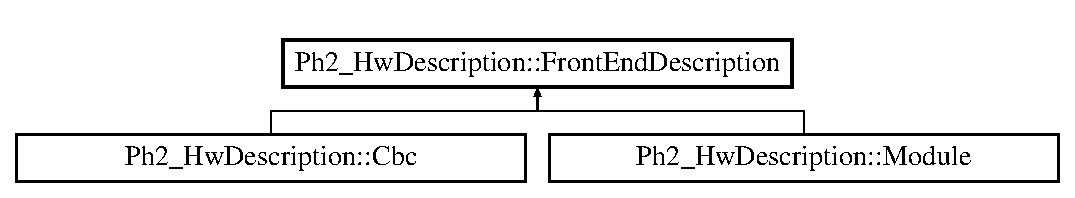
\includegraphics[height=2cm]{class_ph2___hw_description_1_1_front_end_description}
\end{center}
\end{figure}
\subsection*{Public Member Functions}
\begin{CompactItemize}
\item 
\hyperlink{class_ph2___hw_description_1_1_front_end_description_9605f28b75ce29cba767fe6efb9d9d19}{Front\-End\-Description} (uint8\_\-t p\-Shelve\-Id, uint8\_\-t p\-Be\-Id, uint8\_\-t p\-FMCId, uint8\_\-t p\-Fe\-Id, bool p\-Status=true)
\item 
\hyperlink{class_ph2___hw_description_1_1_front_end_description_38c5f465c7227c8cf3f897ab88f9598c}{Front\-End\-Description} (uint8\_\-t p\-Be\-Id, uint8\_\-t p\-FMCId, uint8\_\-t p\-Fe\-Id)
\item 
\hyperlink{class_ph2___hw_description_1_1_front_end_description_3fc1d338b2fb7eca2c8b0038ed235daf}{Front\-End\-Description} ()
\item 
\hyperlink{class_ph2___hw_description_1_1_front_end_description_da01bf978797bf26295f1947b6896efa}{Front\-End\-Description} (const \hyperlink{class_ph2___hw_description_1_1_front_end_description}{Front\-End\-Description} \&p\-Fe\-Desc)
\item 
virtual \hyperlink{class_ph2___hw_description_1_1_front_end_description_8ff5e1dc9dc09e6db9c105a362000e89}{$\sim$Front\-End\-Description} ()
\item 
virtual uint8\_\-t \hyperlink{class_ph2___hw_description_1_1_front_end_description_d38bbaceaee52efe13614561059a0930}{get\-Shelve\-Id} () const 
\begin{CompactList}\small\item\em Get the \hyperlink{class_ph2___hw_description_1_1_shelve}{Shelve} ID. \item\end{CompactList}\item 
virtual uint8\_\-t \hyperlink{class_ph2___hw_description_1_1_front_end_description_093089d617b1a7d4f0b3bf8a83d2eddf}{get\-Be\-Id} () const 
\begin{CompactList}\small\item\em Get the Be ID. \item\end{CompactList}\item 
virtual uint8\_\-t \hyperlink{class_ph2___hw_description_1_1_front_end_description_d5af03f0adc80ee53511ea7e1dfeeea0}{get\-FMCId} () const 
\begin{CompactList}\small\item\em Get the FMC ID. \item\end{CompactList}\item 
virtual uint8\_\-t \hyperlink{class_ph2___hw_description_1_1_front_end_description_e929f2f3d2d8f785506a51e0d9cf44dd}{get\-Fe\-Id} () const 
\begin{CompactList}\small\item\em Get the FE ID. \item\end{CompactList}\item 
virtual bool \hyperlink{class_ph2___hw_description_1_1_front_end_description_867b5c7ff86669819f168cea49539386}{get\-Status} () const 
\begin{CompactList}\small\item\em Get the Status. \item\end{CompactList}\item 
virtual void \hyperlink{class_ph2___hw_description_1_1_front_end_description_b876244bc12be6e5b622f57eccd61c0e}{set\-Shelve\-Id} (uint8\_\-t p\-Shelve\-Id)
\begin{CompactList}\small\item\em Set the \hyperlink{class_ph2___hw_description_1_1_shelve}{Shelve} ID. \item\end{CompactList}\item 
virtual void \hyperlink{class_ph2___hw_description_1_1_front_end_description_f123e6401d5e89f4bf6c52cc23911965}{set\-Be\-Id} (uint8\_\-t p\-Be\-Id)
\begin{CompactList}\small\item\em Set the Be ID. \item\end{CompactList}\item 
virtual void \hyperlink{class_ph2___hw_description_1_1_front_end_description_de9e6abc89ff5c5477584cc58b7c04b2}{set\-FMCId} (uint8\_\-t p\-FMCId)
\begin{CompactList}\small\item\em Set the FMC ID. \item\end{CompactList}\item 
virtual void \hyperlink{class_ph2___hw_description_1_1_front_end_description_99950602e14a271cf1e2fc71be4d9e91}{set\-Fe\-Id} (uint8\_\-t p\-Fe\-Id)
\begin{CompactList}\small\item\em Set the FE ID. \item\end{CompactList}\item 
virtual void \hyperlink{class_ph2___hw_description_1_1_front_end_description_cd0db6c28f72c80079b22ed5da535a40}{set\-Status} (bool p\-Status)
\begin{CompactList}\small\item\em Set the status. \item\end{CompactList}\end{CompactItemize}
\subsection*{Protected Attributes}
\begin{CompactItemize}
\item 
uint8\_\-t \hyperlink{class_ph2___hw_description_1_1_front_end_description_7ce5e0acdcb5647bb94f09ec480e8155}{f\-Shelve\-Id}
\item 
uint8\_\-t \hyperlink{class_ph2___hw_description_1_1_front_end_description_9ad4c11d4b00f0e1325843cfceac2e7c}{f\-Be\-Id}
\item 
uint8\_\-t \hyperlink{class_ph2___hw_description_1_1_front_end_description_4f17ee7ee9d0d395c9f7da5ab3c8f424}{f\-FMCId}
\item 
uint8\_\-t \hyperlink{class_ph2___hw_description_1_1_front_end_description_11b388f8d0f3259e5355779b36e75d9f}{f\-Fe\-Id}
\item 
bool \hyperlink{class_ph2___hw_description_1_1_front_end_description_719dce1ef5c6656fd71ae91f6f404053}{f\-Status}
\end{CompactItemize}


\subsection{Detailed Description}
Describe all parameters common to all FE Components in the DAQ chain. 



\subsection{Constructor \& Destructor Documentation}
\hypertarget{class_ph2___hw_description_1_1_front_end_description_9605f28b75ce29cba767fe6efb9d9d19}{
\index{Ph2_HwDescription::FrontEndDescription@{Ph2\_\-Hw\-Description::Front\-End\-Description}!FrontEndDescription@{FrontEndDescription}}
\index{FrontEndDescription@{FrontEndDescription}!Ph2_HwDescription::FrontEndDescription@{Ph2\_\-Hw\-Description::Front\-End\-Description}}
\subsubsection[FrontEndDescription]{\setlength{\rightskip}{0pt plus 5cm}Ph2\_\-Hw\-Description::Front\-End\-Description::Front\-End\-Description (uint8\_\-t {\em p\-Shelve\-Id}, uint8\_\-t {\em p\-Be\-Id}, uint8\_\-t {\em p\-FMCId}, uint8\_\-t {\em p\-Fe\-Id}, bool {\em p\-Status} = {\tt true})}}
\label{class_ph2___hw_description_1_1_front_end_description_9605f28b75ce29cba767fe6efb9d9d19}


\hypertarget{class_ph2___hw_description_1_1_front_end_description_38c5f465c7227c8cf3f897ab88f9598c}{
\index{Ph2_HwDescription::FrontEndDescription@{Ph2\_\-Hw\-Description::Front\-End\-Description}!FrontEndDescription@{FrontEndDescription}}
\index{FrontEndDescription@{FrontEndDescription}!Ph2_HwDescription::FrontEndDescription@{Ph2\_\-Hw\-Description::Front\-End\-Description}}
\subsubsection[FrontEndDescription]{\setlength{\rightskip}{0pt plus 5cm}Ph2\_\-Hw\-Description::Front\-End\-Description::Front\-End\-Description (uint8\_\-t {\em p\-Be\-Id}, uint8\_\-t {\em p\-FMCId}, uint8\_\-t {\em p\-Fe\-Id})}}
\label{class_ph2___hw_description_1_1_front_end_description_38c5f465c7227c8cf3f897ab88f9598c}


\hypertarget{class_ph2___hw_description_1_1_front_end_description_3fc1d338b2fb7eca2c8b0038ed235daf}{
\index{Ph2_HwDescription::FrontEndDescription@{Ph2\_\-Hw\-Description::Front\-End\-Description}!FrontEndDescription@{FrontEndDescription}}
\index{FrontEndDescription@{FrontEndDescription}!Ph2_HwDescription::FrontEndDescription@{Ph2\_\-Hw\-Description::Front\-End\-Description}}
\subsubsection[FrontEndDescription]{\setlength{\rightskip}{0pt plus 5cm}Ph2\_\-Hw\-Description::Front\-End\-Description::Front\-End\-Description ()}}
\label{class_ph2___hw_description_1_1_front_end_description_3fc1d338b2fb7eca2c8b0038ed235daf}


\hypertarget{class_ph2___hw_description_1_1_front_end_description_da01bf978797bf26295f1947b6896efa}{
\index{Ph2_HwDescription::FrontEndDescription@{Ph2\_\-Hw\-Description::Front\-End\-Description}!FrontEndDescription@{FrontEndDescription}}
\index{FrontEndDescription@{FrontEndDescription}!Ph2_HwDescription::FrontEndDescription@{Ph2\_\-Hw\-Description::Front\-End\-Description}}
\subsubsection[FrontEndDescription]{\setlength{\rightskip}{0pt plus 5cm}Ph2\_\-Hw\-Description::Front\-End\-Description::Front\-End\-Description (const \hyperlink{class_ph2___hw_description_1_1_front_end_description}{Front\-End\-Description} \& {\em p\-Fe\-Desc})}}
\label{class_ph2___hw_description_1_1_front_end_description_da01bf978797bf26295f1947b6896efa}


\hypertarget{class_ph2___hw_description_1_1_front_end_description_8ff5e1dc9dc09e6db9c105a362000e89}{
\index{Ph2_HwDescription::FrontEndDescription@{Ph2\_\-Hw\-Description::Front\-End\-Description}!~FrontEndDescription@{$\sim$FrontEndDescription}}
\index{~FrontEndDescription@{$\sim$FrontEndDescription}!Ph2_HwDescription::FrontEndDescription@{Ph2\_\-Hw\-Description::Front\-End\-Description}}
\subsubsection[$\sim$FrontEndDescription]{\setlength{\rightskip}{0pt plus 5cm}Ph2\_\-Hw\-Description::Front\-End\-Description::$\sim$Front\-End\-Description ()\hspace{0.3cm}{\tt  \mbox{[}virtual\mbox{]}}}}
\label{class_ph2___hw_description_1_1_front_end_description_8ff5e1dc9dc09e6db9c105a362000e89}




\subsection{Member Function Documentation}
\hypertarget{class_ph2___hw_description_1_1_front_end_description_093089d617b1a7d4f0b3bf8a83d2eddf}{
\index{Ph2_HwDescription::FrontEndDescription@{Ph2\_\-Hw\-Description::Front\-End\-Description}!getBeId@{getBeId}}
\index{getBeId@{getBeId}!Ph2_HwDescription::FrontEndDescription@{Ph2\_\-Hw\-Description::Front\-End\-Description}}
\subsubsection[getBeId]{\setlength{\rightskip}{0pt plus 5cm}virtual uint8\_\-t Ph2\_\-Hw\-Description::Front\-End\-Description::get\-Be\-Id () const\hspace{0.3cm}{\tt  \mbox{[}inline, virtual\mbox{]}}}}
\label{class_ph2___hw_description_1_1_front_end_description_093089d617b1a7d4f0b3bf8a83d2eddf}


Get the Be ID. 

\begin{Desc}
\item[Returns:]The Be ID \end{Desc}
\hypertarget{class_ph2___hw_description_1_1_front_end_description_e929f2f3d2d8f785506a51e0d9cf44dd}{
\index{Ph2_HwDescription::FrontEndDescription@{Ph2\_\-Hw\-Description::Front\-End\-Description}!getFeId@{getFeId}}
\index{getFeId@{getFeId}!Ph2_HwDescription::FrontEndDescription@{Ph2\_\-Hw\-Description::Front\-End\-Description}}
\subsubsection[getFeId]{\setlength{\rightskip}{0pt plus 5cm}virtual uint8\_\-t Ph2\_\-Hw\-Description::Front\-End\-Description::get\-Fe\-Id () const\hspace{0.3cm}{\tt  \mbox{[}inline, virtual\mbox{]}}}}
\label{class_ph2___hw_description_1_1_front_end_description_e929f2f3d2d8f785506a51e0d9cf44dd}


Get the FE ID. 

\begin{Desc}
\item[Returns:]The FE ID \end{Desc}
\hypertarget{class_ph2___hw_description_1_1_front_end_description_d5af03f0adc80ee53511ea7e1dfeeea0}{
\index{Ph2_HwDescription::FrontEndDescription@{Ph2\_\-Hw\-Description::Front\-End\-Description}!getFMCId@{getFMCId}}
\index{getFMCId@{getFMCId}!Ph2_HwDescription::FrontEndDescription@{Ph2\_\-Hw\-Description::Front\-End\-Description}}
\subsubsection[getFMCId]{\setlength{\rightskip}{0pt plus 5cm}virtual uint8\_\-t Ph2\_\-Hw\-Description::Front\-End\-Description::get\-FMCId () const\hspace{0.3cm}{\tt  \mbox{[}inline, virtual\mbox{]}}}}
\label{class_ph2___hw_description_1_1_front_end_description_d5af03f0adc80ee53511ea7e1dfeeea0}


Get the FMC ID. 

\begin{Desc}
\item[Returns:]The FMC ID \end{Desc}
\hypertarget{class_ph2___hw_description_1_1_front_end_description_d38bbaceaee52efe13614561059a0930}{
\index{Ph2_HwDescription::FrontEndDescription@{Ph2\_\-Hw\-Description::Front\-End\-Description}!getShelveId@{getShelveId}}
\index{getShelveId@{getShelveId}!Ph2_HwDescription::FrontEndDescription@{Ph2\_\-Hw\-Description::Front\-End\-Description}}
\subsubsection[getShelveId]{\setlength{\rightskip}{0pt plus 5cm}virtual uint8\_\-t Ph2\_\-Hw\-Description::Front\-End\-Description::get\-Shelve\-Id () const\hspace{0.3cm}{\tt  \mbox{[}inline, virtual\mbox{]}}}}
\label{class_ph2___hw_description_1_1_front_end_description_d38bbaceaee52efe13614561059a0930}


Get the \hyperlink{class_ph2___hw_description_1_1_shelve}{Shelve} ID. 

\begin{Desc}
\item[Returns:]The \hyperlink{class_ph2___hw_description_1_1_shelve}{Shelve} ID \end{Desc}
\hypertarget{class_ph2___hw_description_1_1_front_end_description_867b5c7ff86669819f168cea49539386}{
\index{Ph2_HwDescription::FrontEndDescription@{Ph2\_\-Hw\-Description::Front\-End\-Description}!getStatus@{getStatus}}
\index{getStatus@{getStatus}!Ph2_HwDescription::FrontEndDescription@{Ph2\_\-Hw\-Description::Front\-End\-Description}}
\subsubsection[getStatus]{\setlength{\rightskip}{0pt plus 5cm}virtual bool Ph2\_\-Hw\-Description::Front\-End\-Description::get\-Status () const\hspace{0.3cm}{\tt  \mbox{[}inline, virtual\mbox{]}}}}
\label{class_ph2___hw_description_1_1_front_end_description_867b5c7ff86669819f168cea49539386}


Get the Status. 

\begin{Desc}
\item[Returns:]The Status \end{Desc}
\hypertarget{class_ph2___hw_description_1_1_front_end_description_f123e6401d5e89f4bf6c52cc23911965}{
\index{Ph2_HwDescription::FrontEndDescription@{Ph2\_\-Hw\-Description::Front\-End\-Description}!setBeId@{setBeId}}
\index{setBeId@{setBeId}!Ph2_HwDescription::FrontEndDescription@{Ph2\_\-Hw\-Description::Front\-End\-Description}}
\subsubsection[setBeId]{\setlength{\rightskip}{0pt plus 5cm}virtual void Ph2\_\-Hw\-Description::Front\-End\-Description::set\-Be\-Id (uint8\_\-t {\em p\-Be\-Id})\hspace{0.3cm}{\tt  \mbox{[}inline, virtual\mbox{]}}}}
\label{class_ph2___hw_description_1_1_front_end_description_f123e6401d5e89f4bf6c52cc23911965}


Set the Be ID. 

\begin{Desc}
\item[Parameters:]
\begin{description}
\item[{\em p\-Be\-Id}]\end{description}
\end{Desc}
\hypertarget{class_ph2___hw_description_1_1_front_end_description_99950602e14a271cf1e2fc71be4d9e91}{
\index{Ph2_HwDescription::FrontEndDescription@{Ph2\_\-Hw\-Description::Front\-End\-Description}!setFeId@{setFeId}}
\index{setFeId@{setFeId}!Ph2_HwDescription::FrontEndDescription@{Ph2\_\-Hw\-Description::Front\-End\-Description}}
\subsubsection[setFeId]{\setlength{\rightskip}{0pt plus 5cm}virtual void Ph2\_\-Hw\-Description::Front\-End\-Description::set\-Fe\-Id (uint8\_\-t {\em p\-Fe\-Id})\hspace{0.3cm}{\tt  \mbox{[}inline, virtual\mbox{]}}}}
\label{class_ph2___hw_description_1_1_front_end_description_99950602e14a271cf1e2fc71be4d9e91}


Set the FE ID. 

\begin{Desc}
\item[Parameters:]
\begin{description}
\item[{\em p\-Fe\-Id}]\end{description}
\end{Desc}
\hypertarget{class_ph2___hw_description_1_1_front_end_description_de9e6abc89ff5c5477584cc58b7c04b2}{
\index{Ph2_HwDescription::FrontEndDescription@{Ph2\_\-Hw\-Description::Front\-End\-Description}!setFMCId@{setFMCId}}
\index{setFMCId@{setFMCId}!Ph2_HwDescription::FrontEndDescription@{Ph2\_\-Hw\-Description::Front\-End\-Description}}
\subsubsection[setFMCId]{\setlength{\rightskip}{0pt plus 5cm}virtual void Ph2\_\-Hw\-Description::Front\-End\-Description::set\-FMCId (uint8\_\-t {\em p\-FMCId})\hspace{0.3cm}{\tt  \mbox{[}inline, virtual\mbox{]}}}}
\label{class_ph2___hw_description_1_1_front_end_description_de9e6abc89ff5c5477584cc58b7c04b2}


Set the FMC ID. 

\begin{Desc}
\item[Parameters:]
\begin{description}
\item[{\em p\-FMCId}]\end{description}
\end{Desc}
\hypertarget{class_ph2___hw_description_1_1_front_end_description_b876244bc12be6e5b622f57eccd61c0e}{
\index{Ph2_HwDescription::FrontEndDescription@{Ph2\_\-Hw\-Description::Front\-End\-Description}!setShelveId@{setShelveId}}
\index{setShelveId@{setShelveId}!Ph2_HwDescription::FrontEndDescription@{Ph2\_\-Hw\-Description::Front\-End\-Description}}
\subsubsection[setShelveId]{\setlength{\rightskip}{0pt plus 5cm}virtual void Ph2\_\-Hw\-Description::Front\-End\-Description::set\-Shelve\-Id (uint8\_\-t {\em p\-Shelve\-Id})\hspace{0.3cm}{\tt  \mbox{[}inline, virtual\mbox{]}}}}
\label{class_ph2___hw_description_1_1_front_end_description_b876244bc12be6e5b622f57eccd61c0e}


Set the \hyperlink{class_ph2___hw_description_1_1_shelve}{Shelve} ID. 

\begin{Desc}
\item[Parameters:]
\begin{description}
\item[{\em p\-Shelve\-Id}]\end{description}
\end{Desc}
\hypertarget{class_ph2___hw_description_1_1_front_end_description_cd0db6c28f72c80079b22ed5da535a40}{
\index{Ph2_HwDescription::FrontEndDescription@{Ph2\_\-Hw\-Description::Front\-End\-Description}!setStatus@{setStatus}}
\index{setStatus@{setStatus}!Ph2_HwDescription::FrontEndDescription@{Ph2\_\-Hw\-Description::Front\-End\-Description}}
\subsubsection[setStatus]{\setlength{\rightskip}{0pt plus 5cm}virtual void Ph2\_\-Hw\-Description::Front\-End\-Description::set\-Status (bool {\em p\-Status})\hspace{0.3cm}{\tt  \mbox{[}inline, virtual\mbox{]}}}}
\label{class_ph2___hw_description_1_1_front_end_description_cd0db6c28f72c80079b22ed5da535a40}


Set the status. 

\begin{Desc}
\item[Parameters:]
\begin{description}
\item[{\em p\-Status}]\end{description}
\end{Desc}


\subsection{Field Documentation}
\hypertarget{class_ph2___hw_description_1_1_front_end_description_9ad4c11d4b00f0e1325843cfceac2e7c}{
\index{Ph2_HwDescription::FrontEndDescription@{Ph2\_\-Hw\-Description::Front\-End\-Description}!fBeId@{fBeId}}
\index{fBeId@{fBeId}!Ph2_HwDescription::FrontEndDescription@{Ph2\_\-Hw\-Description::Front\-End\-Description}}
\subsubsection[fBeId]{\setlength{\rightskip}{0pt plus 5cm}uint8\_\-t \hyperlink{class_ph2___hw_description_1_1_front_end_description_9ad4c11d4b00f0e1325843cfceac2e7c}{Ph2\_\-Hw\-Description::Front\-End\-Description::f\-Be\-Id}\hspace{0.3cm}{\tt  \mbox{[}protected\mbox{]}}}}
\label{class_ph2___hw_description_1_1_front_end_description_9ad4c11d4b00f0e1325843cfceac2e7c}


\hypertarget{class_ph2___hw_description_1_1_front_end_description_11b388f8d0f3259e5355779b36e75d9f}{
\index{Ph2_HwDescription::FrontEndDescription@{Ph2\_\-Hw\-Description::Front\-End\-Description}!fFeId@{fFeId}}
\index{fFeId@{fFeId}!Ph2_HwDescription::FrontEndDescription@{Ph2\_\-Hw\-Description::Front\-End\-Description}}
\subsubsection[fFeId]{\setlength{\rightskip}{0pt plus 5cm}uint8\_\-t \hyperlink{class_ph2___hw_description_1_1_front_end_description_11b388f8d0f3259e5355779b36e75d9f}{Ph2\_\-Hw\-Description::Front\-End\-Description::f\-Fe\-Id}\hspace{0.3cm}{\tt  \mbox{[}protected\mbox{]}}}}
\label{class_ph2___hw_description_1_1_front_end_description_11b388f8d0f3259e5355779b36e75d9f}


\hypertarget{class_ph2___hw_description_1_1_front_end_description_4f17ee7ee9d0d395c9f7da5ab3c8f424}{
\index{Ph2_HwDescription::FrontEndDescription@{Ph2\_\-Hw\-Description::Front\-End\-Description}!fFMCId@{fFMCId}}
\index{fFMCId@{fFMCId}!Ph2_HwDescription::FrontEndDescription@{Ph2\_\-Hw\-Description::Front\-End\-Description}}
\subsubsection[fFMCId]{\setlength{\rightskip}{0pt plus 5cm}uint8\_\-t \hyperlink{class_ph2___hw_description_1_1_front_end_description_4f17ee7ee9d0d395c9f7da5ab3c8f424}{Ph2\_\-Hw\-Description::Front\-End\-Description::f\-FMCId}\hspace{0.3cm}{\tt  \mbox{[}protected\mbox{]}}}}
\label{class_ph2___hw_description_1_1_front_end_description_4f17ee7ee9d0d395c9f7da5ab3c8f424}


\hypertarget{class_ph2___hw_description_1_1_front_end_description_7ce5e0acdcb5647bb94f09ec480e8155}{
\index{Ph2_HwDescription::FrontEndDescription@{Ph2\_\-Hw\-Description::Front\-End\-Description}!fShelveId@{fShelveId}}
\index{fShelveId@{fShelveId}!Ph2_HwDescription::FrontEndDescription@{Ph2\_\-Hw\-Description::Front\-End\-Description}}
\subsubsection[fShelveId]{\setlength{\rightskip}{0pt plus 5cm}uint8\_\-t \hyperlink{class_ph2___hw_description_1_1_front_end_description_7ce5e0acdcb5647bb94f09ec480e8155}{Ph2\_\-Hw\-Description::Front\-End\-Description::f\-Shelve\-Id}\hspace{0.3cm}{\tt  \mbox{[}protected\mbox{]}}}}
\label{class_ph2___hw_description_1_1_front_end_description_7ce5e0acdcb5647bb94f09ec480e8155}


\hypertarget{class_ph2___hw_description_1_1_front_end_description_719dce1ef5c6656fd71ae91f6f404053}{
\index{Ph2_HwDescription::FrontEndDescription@{Ph2\_\-Hw\-Description::Front\-End\-Description}!fStatus@{fStatus}}
\index{fStatus@{fStatus}!Ph2_HwDescription::FrontEndDescription@{Ph2\_\-Hw\-Description::Front\-End\-Description}}
\subsubsection[fStatus]{\setlength{\rightskip}{0pt plus 5cm}bool \hyperlink{class_ph2___hw_description_1_1_front_end_description_719dce1ef5c6656fd71ae91f6f404053}{Ph2\_\-Hw\-Description::Front\-End\-Description::f\-Status}\hspace{0.3cm}{\tt  \mbox{[}protected\mbox{]}}}}
\label{class_ph2___hw_description_1_1_front_end_description_719dce1ef5c6656fd71ae91f6f404053}




The documentation for this class was generated from the following files:\begin{CompactItemize}
\item 
HWDescription/\hyperlink{_front_end_description_8h}{Front\-End\-Description.h}\item 
HWDescription/\hyperlink{_front_end_description_8cc}{Front\-End\-Description.cc}\end{CompactItemize}

\hypertarget{structgap}{
\section{gap Struct Reference}
\label{structgap}\index{gap@{gap}}
}
\subsection*{Public Member Functions}
\begin{CompactItemize}
\item 
\hyperlink{structgap_4ae36e370647da0df57eb30d3bbcd32b}{gap} ()
\item 
void \hyperlink{structgap_9c0d0b12bc778c8439c8aec7747ab2b0}{push} (char\_\-t $\ast$\&s, size\_\-t count)
\item 
char\_\-t $\ast$ \hyperlink{structgap_176c58ee8d57c41b91ae9f00d5e8cab5}{flush} (char\_\-t $\ast$s)
\end{CompactItemize}
\subsection*{Data Fields}
\begin{CompactItemize}
\item 
char\_\-t $\ast$ \hyperlink{structgap_1fafd4d9909a3413f723f24e46dfde0e}{end}
\item 
size\_\-t \hyperlink{structgap_d5bb3597ade78d89bbe0e300748ad508}{size}
\end{CompactItemize}


\subsection{Constructor \& Destructor Documentation}
\hypertarget{structgap_4ae36e370647da0df57eb30d3bbcd32b}{
\index{gap@{gap}!gap@{gap}}
\index{gap@{gap}!gap@{gap}}
\subsubsection[gap]{\setlength{\rightskip}{0pt plus 5cm}gap::gap ()\hspace{0.3cm}{\tt  \mbox{[}inline\mbox{]}}}}
\label{structgap_4ae36e370647da0df57eb30d3bbcd32b}




\subsection{Member Function Documentation}
\hypertarget{structgap_176c58ee8d57c41b91ae9f00d5e8cab5}{
\index{gap@{gap}!flush@{flush}}
\index{flush@{flush}!gap@{gap}}
\subsubsection[flush]{\setlength{\rightskip}{0pt plus 5cm}char\_\-t$\ast$ gap::flush (char\_\-t $\ast$ {\em s})\hspace{0.3cm}{\tt  \mbox{[}inline\mbox{]}}}}
\label{structgap_176c58ee8d57c41b91ae9f00d5e8cab5}


\hypertarget{structgap_9c0d0b12bc778c8439c8aec7747ab2b0}{
\index{gap@{gap}!push@{push}}
\index{push@{push}!gap@{gap}}
\subsubsection[push]{\setlength{\rightskip}{0pt plus 5cm}void gap::push (char\_\-t $\ast$\& {\em s}, size\_\-t {\em count})\hspace{0.3cm}{\tt  \mbox{[}inline\mbox{]}}}}
\label{structgap_9c0d0b12bc778c8439c8aec7747ab2b0}




\subsection{Field Documentation}
\hypertarget{structgap_1fafd4d9909a3413f723f24e46dfde0e}{
\index{gap@{gap}!end@{end}}
\index{end@{end}!gap@{gap}}
\subsubsection[end]{\setlength{\rightskip}{0pt plus 5cm}char\_\-t$\ast$ \hyperlink{structgap_1fafd4d9909a3413f723f24e46dfde0e}{gap::end}}}
\label{structgap_1fafd4d9909a3413f723f24e46dfde0e}


\hypertarget{structgap_d5bb3597ade78d89bbe0e300748ad508}{
\index{gap@{gap}!size@{size}}
\index{size@{size}!gap@{gap}}
\subsubsection[size]{\setlength{\rightskip}{0pt plus 5cm}size\_\-t \hyperlink{structgap_d5bb3597ade78d89bbe0e300748ad508}{gap::size}}}
\label{structgap_d5bb3597ade78d89bbe0e300748ad508}




The documentation for this struct was generated from the following file:\begin{CompactItemize}
\item 
Utils/\hyperlink{pugixml_8cpp}{pugixml.cpp}\end{CompactItemize}

\hypertarget{class_ph2___hw_interface_1_1_glib_f_w_interface}{\section{Ph2\-\_\-\-Hw\-Interface\-:\-:Glib\-F\-W\-Interface Class Reference}
\label{class_ph2___hw_interface_1_1_glib_f_w_interface}\index{Ph2\-\_\-\-Hw\-Interface\-::\-Glib\-F\-W\-Interface@{Ph2\-\_\-\-Hw\-Interface\-::\-Glib\-F\-W\-Interface}}
}


init/config of the Glib and its Cbc's  




{\ttfamily \#include $<$Glib\-F\-W\-Interface.\-h$>$}

Inheritance diagram for Ph2\-\_\-\-Hw\-Interface\-:\-:Glib\-F\-W\-Interface\-:\begin{figure}[H]
\begin{center}
\leavevmode
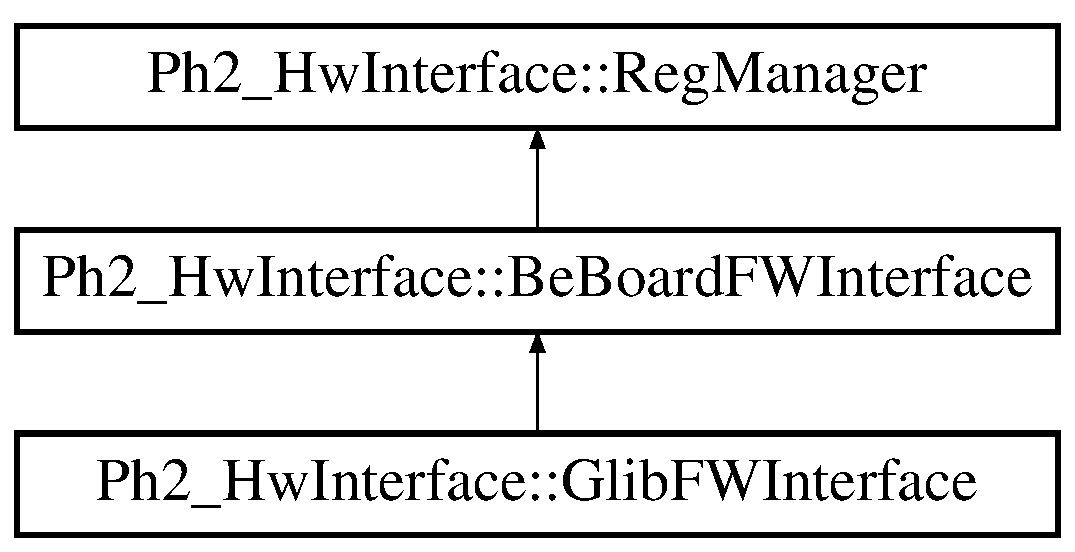
\includegraphics[height=3.000000cm]{class_ph2___hw_interface_1_1_glib_f_w_interface}
\end{center}
\end{figure}
\subsection*{Public Member Functions}
\begin{DoxyCompactItemize}
\item 
\hyperlink{class_ph2___hw_interface_1_1_glib_f_w_interface_aef1044c390e934afa17cdf9566ac71c3}{Glib\-F\-W\-Interface} (const char $\ast$pu\-Hal\-Config\-File\-Name, uint32\-\_\-t p\-Board\-Id)
\begin{DoxyCompactList}\small\item\em Constructor of the \hyperlink{class_ph2___hw_interface_1_1_glib_f_w_interface}{Glib\-F\-W\-Interface} class. \end{DoxyCompactList}\item 
\hyperlink{class_ph2___hw_interface_1_1_glib_f_w_interface_a8cd8fec61b8e8327b142beddcd512b34}{$\sim$\-Glib\-F\-W\-Interface} ()
\begin{DoxyCompactList}\small\item\em Destructor of the \hyperlink{class_ph2___hw_interface_1_1_glib_f_w_interface}{Glib\-F\-W\-Interface} class. \end{DoxyCompactList}\item 
void \hyperlink{class_ph2___hw_interface_1_1_glib_f_w_interface_a52658cd813658d4fae48a79bdabaa5cc}{Configure\-Board} (\hyperlink{class_ph2___hw_description_1_1_be_board}{Be\-Board} $\ast$p\-Board)
\begin{DoxyCompactList}\small\item\em Configure the board with its Config File. \end{DoxyCompactList}\item 
void \hyperlink{class_ph2___hw_interface_1_1_glib_f_w_interface_a2ce120711b8a58610f779813064d2c8f}{Select\-F\-E\-Id} ()
\begin{DoxyCompactList}\small\item\em Detect the right F\-E Id to write the right registers (not working with the latest Firmware) \end{DoxyCompactList}\item 
void \hyperlink{class_ph2___hw_interface_1_1_glib_f_w_interface_adebd47ee3a84dbb8b60f6dd521921aac}{Start} ()
\begin{DoxyCompactList}\small\item\em Start a D\-A\-Q. \end{DoxyCompactList}\item 
void \hyperlink{class_ph2___hw_interface_1_1_glib_f_w_interface_ad980b1ab04d9f87f1a26978201e42997}{Stop} (uint32\-\_\-t p\-Nth\-Acq)
\begin{DoxyCompactList}\small\item\em Stop a D\-A\-Q. \end{DoxyCompactList}\item 
void \hyperlink{class_ph2___hw_interface_1_1_glib_f_w_interface_a05d7f790e0316b51714293e8089086f3}{Pause} ()
\begin{DoxyCompactList}\small\item\em Pause a D\-A\-Q. \end{DoxyCompactList}\item 
void \hyperlink{class_ph2___hw_interface_1_1_glib_f_w_interface_aedd3abfb576016701da27fabc975ac13}{Resume} ()
\begin{DoxyCompactList}\small\item\em Unpause a D\-A\-Q. \end{DoxyCompactList}\item 
void \hyperlink{class_ph2___hw_interface_1_1_glib_f_w_interface_a26c35fec3518f40d09ebc7f0114be19b}{Read\-Data} (\hyperlink{class_ph2___hw_description_1_1_be_board}{Be\-Board} $\ast$p\-Board, uint32\-\_\-t p\-Nth\-Acq, bool p\-Break\-Trigger)
\begin{DoxyCompactList}\small\item\em Read data from D\-A\-Q. \end{DoxyCompactList}\item 
const \hyperlink{class_ph2___hw_interface_1_1_event}{Event} $\ast$ \hyperlink{class_ph2___hw_interface_1_1_glib_f_w_interface_afebeee20cd186f919189e5f349c6a49f}{Get\-Next\-Event} ()
\begin{DoxyCompactList}\small\item\em Get next event from data buffer. \end{DoxyCompactList}\item 
const char $\ast$ \hyperlink{class_ph2___hw_interface_1_1_glib_f_w_interface_a123de5dea8083175ddf299b62861e782}{Get\-Buffer} (uint32\-\_\-t \&p\-Buf\-Size)
\begin{DoxyCompactList}\small\item\em Get the data buffer. \end{DoxyCompactList}\item 
void \hyperlink{class_ph2___hw_interface_1_1_glib_f_w_interface_a2bc165eebeab754425dcbffb21aa2717}{Write\-Cbc\-Block\-Reg} (uint8\-\_\-t p\-Fe\-Id, std\-::vector$<$ uint32\-\_\-t $>$ \&p\-Vec\-Req)
\begin{DoxyCompactList}\small\item\em Read register blocks of a Cbc. \end{DoxyCompactList}\item 
void \hyperlink{class_ph2___hw_interface_1_1_glib_f_w_interface_a9dbc3cf2a991126aed53d834d4d152ce}{Read\-Cbc\-Block\-Reg} (uint8\-\_\-t p\-Fe\-Id, std\-::vector$<$ uint32\-\_\-t $>$ \&p\-Vec\-Req)
\begin{DoxyCompactList}\small\item\em Read register blocks of a Cbc. \end{DoxyCompactList}\end{DoxyCompactItemize}
\subsection*{Private Member Functions}
\begin{DoxyCompactItemize}
\item 
void \hyperlink{class_ph2___hw_interface_1_1_glib_f_w_interface_a0b6b576606e87a52598c3dd3b314c62e}{Select\-Daq\-S\-R\-A\-M} (uint32\-\_\-t p\-Nth\-Acq)
\begin{DoxyCompactList}\small\item\em S\-R\-A\-M selection for D\-A\-Q. \end{DoxyCompactList}\item 
bool \hyperlink{class_ph2___hw_interface_1_1_glib_f_w_interface_aa43ddde3db1e03ed001bda27a2acf7e1}{I2c\-Cmd\-Ack\-Wait} (uint32\-\_\-t p\-Ack\-Val, uint8\-\_\-t p\-Ncount=1)
\begin{DoxyCompactList}\small\item\em Wait for the I2\-C command acknowledgement. \end{DoxyCompactList}\item 
void \hyperlink{class_ph2___hw_interface_1_1_glib_f_w_interface_a17a0f55fc06cc6f0b334f7debcf733d3}{Send\-Block\-Cbc\-I2c\-Request} (std\-::vector$<$ uint32\-\_\-t $>$ \&p\-Vec\-Req, bool p\-Write)
\begin{DoxyCompactList}\small\item\em Send request to r/w blocks via I2\-C. \end{DoxyCompactList}\item 
void \hyperlink{class_ph2___hw_interface_1_1_glib_f_w_interface_ae067b85741fbb52c30a946d5f4f2691b}{Read\-I2c\-Block\-Values\-In\-S\-R\-A\-M} (std\-::vector$<$ uint32\-\_\-t $>$ \&p\-Vec\-Req)
\begin{DoxyCompactList}\small\item\em Read blocks from S\-R\-A\-M via I2\-C. \end{DoxyCompactList}\item 
void \hyperlink{class_ph2___hw_interface_1_1_glib_f_w_interface_abb8f5593c61f54a35a2a7f99b3d6ca55}{Enable\-I2c} (bool p\-Enable)
\begin{DoxyCompactList}\small\item\em Enable I2\-C communications. \end{DoxyCompactList}\item 
void \hyperlink{class_ph2___hw_interface_1_1_glib_f_w_interface_ad7974fd2dee37135dc6cc3997d083037}{Select\-Fe\-S\-R\-A\-M} (uint32\-\_\-t p\-Fe)
\end{DoxyCompactItemize}
\subsection*{Private Attributes}
\begin{DoxyCompactItemize}
\item 
struct timeval \hyperlink{class_ph2___hw_interface_1_1_glib_f_w_interface_a211b2606feb8fad3ac74f00b2d089ade}{f\-Start\-Veto}
\item 
std\-::string \hyperlink{class_ph2___hw_interface_1_1_glib_f_w_interface_a3fd05ec282e3485d13f3d4271f622039}{f\-Str\-Sram}
\item 
std\-::string \hyperlink{class_ph2___hw_interface_1_1_glib_f_w_interface_aee5e3a859a56e2ab7cead5100714851c}{f\-Str\-Sram\-User\-Logic}
\item 
std\-::string \hyperlink{class_ph2___hw_interface_1_1_glib_f_w_interface_a2d5e62e2689d9a0b0ac542ea1ea49b2c}{f\-Str\-Full}
\item 
std\-::string \hyperlink{class_ph2___hw_interface_1_1_glib_f_w_interface_a1c2f018359fc0fc7f9652d6058ac94f1}{f\-Str\-Readout}
\item 
std\-::string \hyperlink{class_ph2___hw_interface_1_1_glib_f_w_interface_a1f3b7bdef0d23e16f014a56aea92209c}{f\-Str\-Other\-Sram}
\item 
std\-::string \hyperlink{class_ph2___hw_interface_1_1_glib_f_w_interface_a875ddab3eef88b4c9b829c1b4bb03d3f}{f\-Str\-Other\-Sram\-User\-Logic}
\item 
std\-::string \hyperlink{class_ph2___hw_interface_1_1_glib_f_w_interface_a96e1ee562be7a0430ec976df840b8b3d}{f\-Cbc\-Stub\-Lat}
\item 
std\-::string \hyperlink{class_ph2___hw_interface_1_1_glib_f_w_interface_aa2c87823ad0d9c2da49526eeef10c8e6}{f\-Cbc\-I2\-C\-Cmd\-Ack}
\item 
std\-::string \hyperlink{class_ph2___hw_interface_1_1_glib_f_w_interface_aa46f35b8ba4a764c83a8cfc1ddf15f1e}{f\-Cbc\-I2\-C\-Cmd\-Rq}
\item 
std\-::string \hyperlink{class_ph2___hw_interface_1_1_glib_f_w_interface_ac7410b226fffc5a361386f6e6c3b96e0}{f\-Cbc\-Hard\-Reset}
\item 
std\-::string \hyperlink{class_ph2___hw_interface_1_1_glib_f_w_interface_a16633bf7e8c4d61cacd8a6862673221c}{f\-Cbc\-Fast\-Reset}
\end{DoxyCompactItemize}
\subsection*{Additional Inherited Members}


\subsection{Detailed Description}
init/config of the Glib and its Cbc's 

\subsection{Constructor \& Destructor Documentation}
\hypertarget{class_ph2___hw_interface_1_1_glib_f_w_interface_aef1044c390e934afa17cdf9566ac71c3}{\index{Ph2\-\_\-\-Hw\-Interface\-::\-Glib\-F\-W\-Interface@{Ph2\-\_\-\-Hw\-Interface\-::\-Glib\-F\-W\-Interface}!Glib\-F\-W\-Interface@{Glib\-F\-W\-Interface}}
\index{Glib\-F\-W\-Interface@{Glib\-F\-W\-Interface}!Ph2_HwInterface::GlibFWInterface@{Ph2\-\_\-\-Hw\-Interface\-::\-Glib\-F\-W\-Interface}}
\subsubsection[{Glib\-F\-W\-Interface}]{\setlength{\rightskip}{0pt plus 5cm}Ph2\-\_\-\-Hw\-Interface\-::\-Glib\-F\-W\-Interface\-::\-Glib\-F\-W\-Interface (
\begin{DoxyParamCaption}
\item[{const char $\ast$}]{pu\-Hal\-Config\-File\-Name, }
\item[{uint32\-\_\-t}]{p\-Board\-Id}
\end{DoxyParamCaption}
)}}\label{class_ph2___hw_interface_1_1_glib_f_w_interface_aef1044c390e934afa17cdf9566ac71c3}


Constructor of the \hyperlink{class_ph2___hw_interface_1_1_glib_f_w_interface}{Glib\-F\-W\-Interface} class. 


\begin{DoxyParams}{Parameters}
{\em pu\-Hal\-Config\-File\-Name} & \-: path of the u\-Hal Config File \\
\hline
{\em p\-Board\-Id} & \\
\hline
\end{DoxyParams}
\hypertarget{class_ph2___hw_interface_1_1_glib_f_w_interface_a8cd8fec61b8e8327b142beddcd512b34}{\index{Ph2\-\_\-\-Hw\-Interface\-::\-Glib\-F\-W\-Interface@{Ph2\-\_\-\-Hw\-Interface\-::\-Glib\-F\-W\-Interface}!$\sim$\-Glib\-F\-W\-Interface@{$\sim$\-Glib\-F\-W\-Interface}}
\index{$\sim$\-Glib\-F\-W\-Interface@{$\sim$\-Glib\-F\-W\-Interface}!Ph2_HwInterface::GlibFWInterface@{Ph2\-\_\-\-Hw\-Interface\-::\-Glib\-F\-W\-Interface}}
\subsubsection[{$\sim$\-Glib\-F\-W\-Interface}]{\setlength{\rightskip}{0pt plus 5cm}Ph2\-\_\-\-Hw\-Interface\-::\-Glib\-F\-W\-Interface\-::$\sim$\-Glib\-F\-W\-Interface (
\begin{DoxyParamCaption}
{}
\end{DoxyParamCaption}
)\hspace{0.3cm}{\ttfamily [inline]}}}\label{class_ph2___hw_interface_1_1_glib_f_w_interface_a8cd8fec61b8e8327b142beddcd512b34}


Destructor of the \hyperlink{class_ph2___hw_interface_1_1_glib_f_w_interface}{Glib\-F\-W\-Interface} class. 



\subsection{Member Function Documentation}
\hypertarget{class_ph2___hw_interface_1_1_glib_f_w_interface_a52658cd813658d4fae48a79bdabaa5cc}{\index{Ph2\-\_\-\-Hw\-Interface\-::\-Glib\-F\-W\-Interface@{Ph2\-\_\-\-Hw\-Interface\-::\-Glib\-F\-W\-Interface}!Configure\-Board@{Configure\-Board}}
\index{Configure\-Board@{Configure\-Board}!Ph2_HwInterface::GlibFWInterface@{Ph2\-\_\-\-Hw\-Interface\-::\-Glib\-F\-W\-Interface}}
\subsubsection[{Configure\-Board}]{\setlength{\rightskip}{0pt plus 5cm}void Ph2\-\_\-\-Hw\-Interface\-::\-Glib\-F\-W\-Interface\-::\-Configure\-Board (
\begin{DoxyParamCaption}
\item[{{\bf Be\-Board} $\ast$}]{p\-Board}
\end{DoxyParamCaption}
)\hspace{0.3cm}{\ttfamily [virtual]}}}\label{class_ph2___hw_interface_1_1_glib_f_w_interface_a52658cd813658d4fae48a79bdabaa5cc}


Configure the board with its Config File. 


\begin{DoxyParams}{Parameters}
{\em p\-Board} & \\
\hline
\end{DoxyParams}


Reimplemented from \hyperlink{class_ph2___hw_interface_1_1_be_board_f_w_interface_a2507c664f19d1d5e3f6de69da16365e8}{Ph2\-\_\-\-Hw\-Interface\-::\-Be\-Board\-F\-W\-Interface}.

\hypertarget{class_ph2___hw_interface_1_1_glib_f_w_interface_abb8f5593c61f54a35a2a7f99b3d6ca55}{\index{Ph2\-\_\-\-Hw\-Interface\-::\-Glib\-F\-W\-Interface@{Ph2\-\_\-\-Hw\-Interface\-::\-Glib\-F\-W\-Interface}!Enable\-I2c@{Enable\-I2c}}
\index{Enable\-I2c@{Enable\-I2c}!Ph2_HwInterface::GlibFWInterface@{Ph2\-\_\-\-Hw\-Interface\-::\-Glib\-F\-W\-Interface}}
\subsubsection[{Enable\-I2c}]{\setlength{\rightskip}{0pt plus 5cm}void Ph2\-\_\-\-Hw\-Interface\-::\-Glib\-F\-W\-Interface\-::\-Enable\-I2c (
\begin{DoxyParamCaption}
\item[{bool}]{p\-Enable}
\end{DoxyParamCaption}
)\hspace{0.3cm}{\ttfamily [private]}}}\label{class_ph2___hw_interface_1_1_glib_f_w_interface_abb8f5593c61f54a35a2a7f99b3d6ca55}


Enable I2\-C communications. 


\begin{DoxyParams}{Parameters}
{\em p\-Enable} & \-: 1/0 -\/$>$ Enable/\-Disable \\
\hline
\end{DoxyParams}
\hypertarget{class_ph2___hw_interface_1_1_glib_f_w_interface_a123de5dea8083175ddf299b62861e782}{\index{Ph2\-\_\-\-Hw\-Interface\-::\-Glib\-F\-W\-Interface@{Ph2\-\_\-\-Hw\-Interface\-::\-Glib\-F\-W\-Interface}!Get\-Buffer@{Get\-Buffer}}
\index{Get\-Buffer@{Get\-Buffer}!Ph2_HwInterface::GlibFWInterface@{Ph2\-\_\-\-Hw\-Interface\-::\-Glib\-F\-W\-Interface}}
\subsubsection[{Get\-Buffer}]{\setlength{\rightskip}{0pt plus 5cm}const char $\ast$ Ph2\-\_\-\-Hw\-Interface\-::\-Glib\-F\-W\-Interface\-::\-Get\-Buffer (
\begin{DoxyParamCaption}
\item[{uint32\-\_\-t \&}]{p\-Buf\-Size}
\end{DoxyParamCaption}
)}}\label{class_ph2___hw_interface_1_1_glib_f_w_interface_a123de5dea8083175ddf299b62861e782}


Get the data buffer. 


\begin{DoxyParams}{Parameters}
{\em p\-Buf\-Size} & \-: recovers the data buffer size \\
\hline
\end{DoxyParams}
\begin{DoxyReturn}{Returns}
\hyperlink{class_ph2___hw_interface_1_1_data}{Data} buffer 
\end{DoxyReturn}
\hypertarget{class_ph2___hw_interface_1_1_glib_f_w_interface_afebeee20cd186f919189e5f349c6a49f}{\index{Ph2\-\_\-\-Hw\-Interface\-::\-Glib\-F\-W\-Interface@{Ph2\-\_\-\-Hw\-Interface\-::\-Glib\-F\-W\-Interface}!Get\-Next\-Event@{Get\-Next\-Event}}
\index{Get\-Next\-Event@{Get\-Next\-Event}!Ph2_HwInterface::GlibFWInterface@{Ph2\-\_\-\-Hw\-Interface\-::\-Glib\-F\-W\-Interface}}
\subsubsection[{Get\-Next\-Event}]{\setlength{\rightskip}{0pt plus 5cm}const {\bf Event} $\ast$ Ph2\-\_\-\-Hw\-Interface\-::\-Glib\-F\-W\-Interface\-::\-Get\-Next\-Event (
\begin{DoxyParamCaption}
{}
\end{DoxyParamCaption}
)\hspace{0.3cm}{\ttfamily [virtual]}}}\label{class_ph2___hw_interface_1_1_glib_f_w_interface_afebeee20cd186f919189e5f349c6a49f}


Get next event from data buffer. 

\begin{DoxyReturn}{Returns}
Next event 
\end{DoxyReturn}


Reimplemented from \hyperlink{class_ph2___hw_interface_1_1_be_board_f_w_interface_a5f524d2a377db09667de71563e0fab3d}{Ph2\-\_\-\-Hw\-Interface\-::\-Be\-Board\-F\-W\-Interface}.

\hypertarget{class_ph2___hw_interface_1_1_glib_f_w_interface_aa43ddde3db1e03ed001bda27a2acf7e1}{\index{Ph2\-\_\-\-Hw\-Interface\-::\-Glib\-F\-W\-Interface@{Ph2\-\_\-\-Hw\-Interface\-::\-Glib\-F\-W\-Interface}!I2c\-Cmd\-Ack\-Wait@{I2c\-Cmd\-Ack\-Wait}}
\index{I2c\-Cmd\-Ack\-Wait@{I2c\-Cmd\-Ack\-Wait}!Ph2_HwInterface::GlibFWInterface@{Ph2\-\_\-\-Hw\-Interface\-::\-Glib\-F\-W\-Interface}}
\subsubsection[{I2c\-Cmd\-Ack\-Wait}]{\setlength{\rightskip}{0pt plus 5cm}bool Ph2\-\_\-\-Hw\-Interface\-::\-Glib\-F\-W\-Interface\-::\-I2c\-Cmd\-Ack\-Wait (
\begin{DoxyParamCaption}
\item[{uint32\-\_\-t}]{p\-Ack\-Val, }
\item[{uint8\-\_\-t}]{p\-Ncount = {\ttfamily 1}}
\end{DoxyParamCaption}
)\hspace{0.3cm}{\ttfamily [private]}}}\label{class_ph2___hw_interface_1_1_glib_f_w_interface_aa43ddde3db1e03ed001bda27a2acf7e1}


Wait for the I2\-C command acknowledgement. 


\begin{DoxyParams}{Parameters}
{\em p\-Ack\-Val} & \-: Expected status of acknowledgement, 1/0 -\/$>$ true/false \\
\hline
{\em p\-Ncount} & \-: Number of registers at stake \\
\hline
\end{DoxyParams}
\begin{DoxyReturn}{Returns}
boolean confirming the acknowledgement 
\end{DoxyReturn}
\hypertarget{class_ph2___hw_interface_1_1_glib_f_w_interface_a05d7f790e0316b51714293e8089086f3}{\index{Ph2\-\_\-\-Hw\-Interface\-::\-Glib\-F\-W\-Interface@{Ph2\-\_\-\-Hw\-Interface\-::\-Glib\-F\-W\-Interface}!Pause@{Pause}}
\index{Pause@{Pause}!Ph2_HwInterface::GlibFWInterface@{Ph2\-\_\-\-Hw\-Interface\-::\-Glib\-F\-W\-Interface}}
\subsubsection[{Pause}]{\setlength{\rightskip}{0pt plus 5cm}void Ph2\-\_\-\-Hw\-Interface\-::\-Glib\-F\-W\-Interface\-::\-Pause (
\begin{DoxyParamCaption}
{}
\end{DoxyParamCaption}
)\hspace{0.3cm}{\ttfamily [virtual]}}}\label{class_ph2___hw_interface_1_1_glib_f_w_interface_a05d7f790e0316b51714293e8089086f3}


Pause a D\-A\-Q. 



Reimplemented from \hyperlink{class_ph2___hw_interface_1_1_be_board_f_w_interface_afb21d1663b328272c12cab6970114ecd}{Ph2\-\_\-\-Hw\-Interface\-::\-Be\-Board\-F\-W\-Interface}.

\hypertarget{class_ph2___hw_interface_1_1_glib_f_w_interface_a9dbc3cf2a991126aed53d834d4d152ce}{\index{Ph2\-\_\-\-Hw\-Interface\-::\-Glib\-F\-W\-Interface@{Ph2\-\_\-\-Hw\-Interface\-::\-Glib\-F\-W\-Interface}!Read\-Cbc\-Block\-Reg@{Read\-Cbc\-Block\-Reg}}
\index{Read\-Cbc\-Block\-Reg@{Read\-Cbc\-Block\-Reg}!Ph2_HwInterface::GlibFWInterface@{Ph2\-\_\-\-Hw\-Interface\-::\-Glib\-F\-W\-Interface}}
\subsubsection[{Read\-Cbc\-Block\-Reg}]{\setlength{\rightskip}{0pt plus 5cm}void Ph2\-\_\-\-Hw\-Interface\-::\-Glib\-F\-W\-Interface\-::\-Read\-Cbc\-Block\-Reg (
\begin{DoxyParamCaption}
\item[{uint8\-\_\-t}]{p\-Fe\-Id, }
\item[{std\-::vector$<$ uint32\-\_\-t $>$ \&}]{p\-Vec\-Req}
\end{DoxyParamCaption}
)\hspace{0.3cm}{\ttfamily [virtual]}}}\label{class_ph2___hw_interface_1_1_glib_f_w_interface_a9dbc3cf2a991126aed53d834d4d152ce}


Read register blocks of a Cbc. 


\begin{DoxyParams}{Parameters}
{\em p\-Fe\-Id} & \-: Front\-End to work with \\
\hline
{\em p\-Vec\-Req} & \-: Vector to stack the read words \\
\hline
\end{DoxyParams}


Reimplemented from \hyperlink{class_ph2___hw_interface_1_1_be_board_f_w_interface_a624e0ef864d5bdef907041270d04bffb}{Ph2\-\_\-\-Hw\-Interface\-::\-Be\-Board\-F\-W\-Interface}.

\hypertarget{class_ph2___hw_interface_1_1_glib_f_w_interface_a26c35fec3518f40d09ebc7f0114be19b}{\index{Ph2\-\_\-\-Hw\-Interface\-::\-Glib\-F\-W\-Interface@{Ph2\-\_\-\-Hw\-Interface\-::\-Glib\-F\-W\-Interface}!Read\-Data@{Read\-Data}}
\index{Read\-Data@{Read\-Data}!Ph2_HwInterface::GlibFWInterface@{Ph2\-\_\-\-Hw\-Interface\-::\-Glib\-F\-W\-Interface}}
\subsubsection[{Read\-Data}]{\setlength{\rightskip}{0pt plus 5cm}void Ph2\-\_\-\-Hw\-Interface\-::\-Glib\-F\-W\-Interface\-::\-Read\-Data (
\begin{DoxyParamCaption}
\item[{{\bf Be\-Board} $\ast$}]{p\-Board, }
\item[{uint32\-\_\-t}]{p\-Nth\-Acq, }
\item[{bool}]{p\-Break\-Trigger}
\end{DoxyParamCaption}
)\hspace{0.3cm}{\ttfamily [virtual]}}}\label{class_ph2___hw_interface_1_1_glib_f_w_interface_a26c35fec3518f40d09ebc7f0114be19b}


Read data from D\-A\-Q. 


\begin{DoxyParams}{Parameters}
{\em p\-Nth\-Acq} & \-: actual number of acquisitions \\
\hline
{\em p\-Break\-Trigger} & \-: if true, enable the break trigger \\
\hline
\end{DoxyParams}


Reimplemented from \hyperlink{class_ph2___hw_interface_1_1_be_board_f_w_interface_af27f2a01b7625d2b144760413128acf2}{Ph2\-\_\-\-Hw\-Interface\-::\-Be\-Board\-F\-W\-Interface}.

\hypertarget{class_ph2___hw_interface_1_1_glib_f_w_interface_ae067b85741fbb52c30a946d5f4f2691b}{\index{Ph2\-\_\-\-Hw\-Interface\-::\-Glib\-F\-W\-Interface@{Ph2\-\_\-\-Hw\-Interface\-::\-Glib\-F\-W\-Interface}!Read\-I2c\-Block\-Values\-In\-S\-R\-A\-M@{Read\-I2c\-Block\-Values\-In\-S\-R\-A\-M}}
\index{Read\-I2c\-Block\-Values\-In\-S\-R\-A\-M@{Read\-I2c\-Block\-Values\-In\-S\-R\-A\-M}!Ph2_HwInterface::GlibFWInterface@{Ph2\-\_\-\-Hw\-Interface\-::\-Glib\-F\-W\-Interface}}
\subsubsection[{Read\-I2c\-Block\-Values\-In\-S\-R\-A\-M}]{\setlength{\rightskip}{0pt plus 5cm}void Ph2\-\_\-\-Hw\-Interface\-::\-Glib\-F\-W\-Interface\-::\-Read\-I2c\-Block\-Values\-In\-S\-R\-A\-M (
\begin{DoxyParamCaption}
\item[{std\-::vector$<$ uint32\-\_\-t $>$ \&}]{p\-Vec\-Req}
\end{DoxyParamCaption}
)\hspace{0.3cm}{\ttfamily [private]}}}\label{class_ph2___hw_interface_1_1_glib_f_w_interface_ae067b85741fbb52c30a946d5f4f2691b}


Read blocks from S\-R\-A\-M via I2\-C. 


\begin{DoxyParams}{Parameters}
{\em p\-Vec\-Req} & \-: Vector to stack the read words \\
\hline
\end{DoxyParams}
\hypertarget{class_ph2___hw_interface_1_1_glib_f_w_interface_aedd3abfb576016701da27fabc975ac13}{\index{Ph2\-\_\-\-Hw\-Interface\-::\-Glib\-F\-W\-Interface@{Ph2\-\_\-\-Hw\-Interface\-::\-Glib\-F\-W\-Interface}!Resume@{Resume}}
\index{Resume@{Resume}!Ph2_HwInterface::GlibFWInterface@{Ph2\-\_\-\-Hw\-Interface\-::\-Glib\-F\-W\-Interface}}
\subsubsection[{Resume}]{\setlength{\rightskip}{0pt plus 5cm}void Ph2\-\_\-\-Hw\-Interface\-::\-Glib\-F\-W\-Interface\-::\-Resume (
\begin{DoxyParamCaption}
{}
\end{DoxyParamCaption}
)\hspace{0.3cm}{\ttfamily [virtual]}}}\label{class_ph2___hw_interface_1_1_glib_f_w_interface_aedd3abfb576016701da27fabc975ac13}


Unpause a D\-A\-Q. 



Reimplemented from \hyperlink{class_ph2___hw_interface_1_1_be_board_f_w_interface_aafa48fcae2c37040141afc89113881e5}{Ph2\-\_\-\-Hw\-Interface\-::\-Be\-Board\-F\-W\-Interface}.

\hypertarget{class_ph2___hw_interface_1_1_glib_f_w_interface_a0b6b576606e87a52598c3dd3b314c62e}{\index{Ph2\-\_\-\-Hw\-Interface\-::\-Glib\-F\-W\-Interface@{Ph2\-\_\-\-Hw\-Interface\-::\-Glib\-F\-W\-Interface}!Select\-Daq\-S\-R\-A\-M@{Select\-Daq\-S\-R\-A\-M}}
\index{Select\-Daq\-S\-R\-A\-M@{Select\-Daq\-S\-R\-A\-M}!Ph2_HwInterface::GlibFWInterface@{Ph2\-\_\-\-Hw\-Interface\-::\-Glib\-F\-W\-Interface}}
\subsubsection[{Select\-Daq\-S\-R\-A\-M}]{\setlength{\rightskip}{0pt plus 5cm}void Ph2\-\_\-\-Hw\-Interface\-::\-Glib\-F\-W\-Interface\-::\-Select\-Daq\-S\-R\-A\-M (
\begin{DoxyParamCaption}
\item[{uint32\-\_\-t}]{p\-Nth\-Acq}
\end{DoxyParamCaption}
)\hspace{0.3cm}{\ttfamily [private]}}}\label{class_ph2___hw_interface_1_1_glib_f_w_interface_a0b6b576606e87a52598c3dd3b314c62e}


S\-R\-A\-M selection for D\-A\-Q. 


\begin{DoxyParams}{Parameters}
{\em p\-Nth\-Acq} & \-: actual number of acquisitions \\
\hline
\end{DoxyParams}
\hypertarget{class_ph2___hw_interface_1_1_glib_f_w_interface_a2ce120711b8a58610f779813064d2c8f}{\index{Ph2\-\_\-\-Hw\-Interface\-::\-Glib\-F\-W\-Interface@{Ph2\-\_\-\-Hw\-Interface\-::\-Glib\-F\-W\-Interface}!Select\-F\-E\-Id@{Select\-F\-E\-Id}}
\index{Select\-F\-E\-Id@{Select\-F\-E\-Id}!Ph2_HwInterface::GlibFWInterface@{Ph2\-\_\-\-Hw\-Interface\-::\-Glib\-F\-W\-Interface}}
\subsubsection[{Select\-F\-E\-Id}]{\setlength{\rightskip}{0pt plus 5cm}void Ph2\-\_\-\-Hw\-Interface\-::\-Glib\-F\-W\-Interface\-::\-Select\-F\-E\-Id (
\begin{DoxyParamCaption}
{}
\end{DoxyParamCaption}
)}}\label{class_ph2___hw_interface_1_1_glib_f_w_interface_a2ce120711b8a58610f779813064d2c8f}


Detect the right F\-E Id to write the right registers (not working with the latest Firmware) 

\hypertarget{class_ph2___hw_interface_1_1_glib_f_w_interface_ad7974fd2dee37135dc6cc3997d083037}{\index{Ph2\-\_\-\-Hw\-Interface\-::\-Glib\-F\-W\-Interface@{Ph2\-\_\-\-Hw\-Interface\-::\-Glib\-F\-W\-Interface}!Select\-Fe\-S\-R\-A\-M@{Select\-Fe\-S\-R\-A\-M}}
\index{Select\-Fe\-S\-R\-A\-M@{Select\-Fe\-S\-R\-A\-M}!Ph2_HwInterface::GlibFWInterface@{Ph2\-\_\-\-Hw\-Interface\-::\-Glib\-F\-W\-Interface}}
\subsubsection[{Select\-Fe\-S\-R\-A\-M}]{\setlength{\rightskip}{0pt plus 5cm}void Ph2\-\_\-\-Hw\-Interface\-::\-Glib\-F\-W\-Interface\-::\-Select\-Fe\-S\-R\-A\-M (
\begin{DoxyParamCaption}
\item[{uint32\-\_\-t}]{p\-Fe}
\end{DoxyParamCaption}
)\hspace{0.3cm}{\ttfamily [private]}}}\label{class_ph2___hw_interface_1_1_glib_f_w_interface_ad7974fd2dee37135dc6cc3997d083037}
\hypertarget{class_ph2___hw_interface_1_1_glib_f_w_interface_a17a0f55fc06cc6f0b334f7debcf733d3}{\index{Ph2\-\_\-\-Hw\-Interface\-::\-Glib\-F\-W\-Interface@{Ph2\-\_\-\-Hw\-Interface\-::\-Glib\-F\-W\-Interface}!Send\-Block\-Cbc\-I2c\-Request@{Send\-Block\-Cbc\-I2c\-Request}}
\index{Send\-Block\-Cbc\-I2c\-Request@{Send\-Block\-Cbc\-I2c\-Request}!Ph2_HwInterface::GlibFWInterface@{Ph2\-\_\-\-Hw\-Interface\-::\-Glib\-F\-W\-Interface}}
\subsubsection[{Send\-Block\-Cbc\-I2c\-Request}]{\setlength{\rightskip}{0pt plus 5cm}void Ph2\-\_\-\-Hw\-Interface\-::\-Glib\-F\-W\-Interface\-::\-Send\-Block\-Cbc\-I2c\-Request (
\begin{DoxyParamCaption}
\item[{std\-::vector$<$ uint32\-\_\-t $>$ \&}]{p\-Vec\-Req, }
\item[{bool}]{p\-Write}
\end{DoxyParamCaption}
)\hspace{0.3cm}{\ttfamily [private]}}}\label{class_ph2___hw_interface_1_1_glib_f_w_interface_a17a0f55fc06cc6f0b334f7debcf733d3}


Send request to r/w blocks via I2\-C. 


\begin{DoxyParams}{Parameters}
{\em p\-Vec\-Req} & \-: Block of words to send \\
\hline
{\em p\-Write} & \-: 1/0 -\/$>$ Write/\-Read \\
\hline
\end{DoxyParams}
\hypertarget{class_ph2___hw_interface_1_1_glib_f_w_interface_adebd47ee3a84dbb8b60f6dd521921aac}{\index{Ph2\-\_\-\-Hw\-Interface\-::\-Glib\-F\-W\-Interface@{Ph2\-\_\-\-Hw\-Interface\-::\-Glib\-F\-W\-Interface}!Start@{Start}}
\index{Start@{Start}!Ph2_HwInterface::GlibFWInterface@{Ph2\-\_\-\-Hw\-Interface\-::\-Glib\-F\-W\-Interface}}
\subsubsection[{Start}]{\setlength{\rightskip}{0pt plus 5cm}void Ph2\-\_\-\-Hw\-Interface\-::\-Glib\-F\-W\-Interface\-::\-Start (
\begin{DoxyParamCaption}
{}
\end{DoxyParamCaption}
)\hspace{0.3cm}{\ttfamily [virtual]}}}\label{class_ph2___hw_interface_1_1_glib_f_w_interface_adebd47ee3a84dbb8b60f6dd521921aac}


Start a D\-A\-Q. 



Reimplemented from \hyperlink{class_ph2___hw_interface_1_1_be_board_f_w_interface_a2835dae7ec6788c1d5728e53f9c3051a}{Ph2\-\_\-\-Hw\-Interface\-::\-Be\-Board\-F\-W\-Interface}.

\hypertarget{class_ph2___hw_interface_1_1_glib_f_w_interface_ad980b1ab04d9f87f1a26978201e42997}{\index{Ph2\-\_\-\-Hw\-Interface\-::\-Glib\-F\-W\-Interface@{Ph2\-\_\-\-Hw\-Interface\-::\-Glib\-F\-W\-Interface}!Stop@{Stop}}
\index{Stop@{Stop}!Ph2_HwInterface::GlibFWInterface@{Ph2\-\_\-\-Hw\-Interface\-::\-Glib\-F\-W\-Interface}}
\subsubsection[{Stop}]{\setlength{\rightskip}{0pt plus 5cm}void Ph2\-\_\-\-Hw\-Interface\-::\-Glib\-F\-W\-Interface\-::\-Stop (
\begin{DoxyParamCaption}
\item[{uint32\-\_\-t}]{p\-Nth\-Acq}
\end{DoxyParamCaption}
)\hspace{0.3cm}{\ttfamily [virtual]}}}\label{class_ph2___hw_interface_1_1_glib_f_w_interface_ad980b1ab04d9f87f1a26978201e42997}


Stop a D\-A\-Q. 


\begin{DoxyParams}{Parameters}
{\em p\-Nth\-Acq} & \-: actual number of acquisitions \\
\hline
\end{DoxyParams}


Reimplemented from \hyperlink{class_ph2___hw_interface_1_1_be_board_f_w_interface_af7825e291796f7c8c498a92365583e08}{Ph2\-\_\-\-Hw\-Interface\-::\-Be\-Board\-F\-W\-Interface}.

\hypertarget{class_ph2___hw_interface_1_1_glib_f_w_interface_a2bc165eebeab754425dcbffb21aa2717}{\index{Ph2\-\_\-\-Hw\-Interface\-::\-Glib\-F\-W\-Interface@{Ph2\-\_\-\-Hw\-Interface\-::\-Glib\-F\-W\-Interface}!Write\-Cbc\-Block\-Reg@{Write\-Cbc\-Block\-Reg}}
\index{Write\-Cbc\-Block\-Reg@{Write\-Cbc\-Block\-Reg}!Ph2_HwInterface::GlibFWInterface@{Ph2\-\_\-\-Hw\-Interface\-::\-Glib\-F\-W\-Interface}}
\subsubsection[{Write\-Cbc\-Block\-Reg}]{\setlength{\rightskip}{0pt plus 5cm}void Ph2\-\_\-\-Hw\-Interface\-::\-Glib\-F\-W\-Interface\-::\-Write\-Cbc\-Block\-Reg (
\begin{DoxyParamCaption}
\item[{uint8\-\_\-t}]{p\-Fe\-Id, }
\item[{std\-::vector$<$ uint32\-\_\-t $>$ \&}]{p\-Vec\-Req}
\end{DoxyParamCaption}
)\hspace{0.3cm}{\ttfamily [virtual]}}}\label{class_ph2___hw_interface_1_1_glib_f_w_interface_a2bc165eebeab754425dcbffb21aa2717}


Read register blocks of a Cbc. 


\begin{DoxyParams}{Parameters}
{\em p\-Fe\-Id} & \-: Front\-End to work with \\
\hline
{\em p\-Vec\-Req} & \-: Vector to stack the read words \\
\hline
\end{DoxyParams}


Reimplemented from \hyperlink{class_ph2___hw_interface_1_1_be_board_f_w_interface_aea9e44d8b6de6bd204b74eeafba00f7c}{Ph2\-\_\-\-Hw\-Interface\-::\-Be\-Board\-F\-W\-Interface}.



\subsection{Field Documentation}
\hypertarget{class_ph2___hw_interface_1_1_glib_f_w_interface_a16633bf7e8c4d61cacd8a6862673221c}{\index{Ph2\-\_\-\-Hw\-Interface\-::\-Glib\-F\-W\-Interface@{Ph2\-\_\-\-Hw\-Interface\-::\-Glib\-F\-W\-Interface}!f\-Cbc\-Fast\-Reset@{f\-Cbc\-Fast\-Reset}}
\index{f\-Cbc\-Fast\-Reset@{f\-Cbc\-Fast\-Reset}!Ph2_HwInterface::GlibFWInterface@{Ph2\-\_\-\-Hw\-Interface\-::\-Glib\-F\-W\-Interface}}
\subsubsection[{f\-Cbc\-Fast\-Reset}]{\setlength{\rightskip}{0pt plus 5cm}std\-::string Ph2\-\_\-\-Hw\-Interface\-::\-Glib\-F\-W\-Interface\-::f\-Cbc\-Fast\-Reset\hspace{0.3cm}{\ttfamily [private]}}}\label{class_ph2___hw_interface_1_1_glib_f_w_interface_a16633bf7e8c4d61cacd8a6862673221c}
\hypertarget{class_ph2___hw_interface_1_1_glib_f_w_interface_ac7410b226fffc5a361386f6e6c3b96e0}{\index{Ph2\-\_\-\-Hw\-Interface\-::\-Glib\-F\-W\-Interface@{Ph2\-\_\-\-Hw\-Interface\-::\-Glib\-F\-W\-Interface}!f\-Cbc\-Hard\-Reset@{f\-Cbc\-Hard\-Reset}}
\index{f\-Cbc\-Hard\-Reset@{f\-Cbc\-Hard\-Reset}!Ph2_HwInterface::GlibFWInterface@{Ph2\-\_\-\-Hw\-Interface\-::\-Glib\-F\-W\-Interface}}
\subsubsection[{f\-Cbc\-Hard\-Reset}]{\setlength{\rightskip}{0pt plus 5cm}std\-::string Ph2\-\_\-\-Hw\-Interface\-::\-Glib\-F\-W\-Interface\-::f\-Cbc\-Hard\-Reset\hspace{0.3cm}{\ttfamily [private]}}}\label{class_ph2___hw_interface_1_1_glib_f_w_interface_ac7410b226fffc5a361386f6e6c3b96e0}
\hypertarget{class_ph2___hw_interface_1_1_glib_f_w_interface_aa2c87823ad0d9c2da49526eeef10c8e6}{\index{Ph2\-\_\-\-Hw\-Interface\-::\-Glib\-F\-W\-Interface@{Ph2\-\_\-\-Hw\-Interface\-::\-Glib\-F\-W\-Interface}!f\-Cbc\-I2\-C\-Cmd\-Ack@{f\-Cbc\-I2\-C\-Cmd\-Ack}}
\index{f\-Cbc\-I2\-C\-Cmd\-Ack@{f\-Cbc\-I2\-C\-Cmd\-Ack}!Ph2_HwInterface::GlibFWInterface@{Ph2\-\_\-\-Hw\-Interface\-::\-Glib\-F\-W\-Interface}}
\subsubsection[{f\-Cbc\-I2\-C\-Cmd\-Ack}]{\setlength{\rightskip}{0pt plus 5cm}std\-::string Ph2\-\_\-\-Hw\-Interface\-::\-Glib\-F\-W\-Interface\-::f\-Cbc\-I2\-C\-Cmd\-Ack\hspace{0.3cm}{\ttfamily [private]}}}\label{class_ph2___hw_interface_1_1_glib_f_w_interface_aa2c87823ad0d9c2da49526eeef10c8e6}
\hypertarget{class_ph2___hw_interface_1_1_glib_f_w_interface_aa46f35b8ba4a764c83a8cfc1ddf15f1e}{\index{Ph2\-\_\-\-Hw\-Interface\-::\-Glib\-F\-W\-Interface@{Ph2\-\_\-\-Hw\-Interface\-::\-Glib\-F\-W\-Interface}!f\-Cbc\-I2\-C\-Cmd\-Rq@{f\-Cbc\-I2\-C\-Cmd\-Rq}}
\index{f\-Cbc\-I2\-C\-Cmd\-Rq@{f\-Cbc\-I2\-C\-Cmd\-Rq}!Ph2_HwInterface::GlibFWInterface@{Ph2\-\_\-\-Hw\-Interface\-::\-Glib\-F\-W\-Interface}}
\subsubsection[{f\-Cbc\-I2\-C\-Cmd\-Rq}]{\setlength{\rightskip}{0pt plus 5cm}std\-::string Ph2\-\_\-\-Hw\-Interface\-::\-Glib\-F\-W\-Interface\-::f\-Cbc\-I2\-C\-Cmd\-Rq\hspace{0.3cm}{\ttfamily [private]}}}\label{class_ph2___hw_interface_1_1_glib_f_w_interface_aa46f35b8ba4a764c83a8cfc1ddf15f1e}
\hypertarget{class_ph2___hw_interface_1_1_glib_f_w_interface_a96e1ee562be7a0430ec976df840b8b3d}{\index{Ph2\-\_\-\-Hw\-Interface\-::\-Glib\-F\-W\-Interface@{Ph2\-\_\-\-Hw\-Interface\-::\-Glib\-F\-W\-Interface}!f\-Cbc\-Stub\-Lat@{f\-Cbc\-Stub\-Lat}}
\index{f\-Cbc\-Stub\-Lat@{f\-Cbc\-Stub\-Lat}!Ph2_HwInterface::GlibFWInterface@{Ph2\-\_\-\-Hw\-Interface\-::\-Glib\-F\-W\-Interface}}
\subsubsection[{f\-Cbc\-Stub\-Lat}]{\setlength{\rightskip}{0pt plus 5cm}std\-::string Ph2\-\_\-\-Hw\-Interface\-::\-Glib\-F\-W\-Interface\-::f\-Cbc\-Stub\-Lat\hspace{0.3cm}{\ttfamily [private]}}}\label{class_ph2___hw_interface_1_1_glib_f_w_interface_a96e1ee562be7a0430ec976df840b8b3d}
\hypertarget{class_ph2___hw_interface_1_1_glib_f_w_interface_a211b2606feb8fad3ac74f00b2d089ade}{\index{Ph2\-\_\-\-Hw\-Interface\-::\-Glib\-F\-W\-Interface@{Ph2\-\_\-\-Hw\-Interface\-::\-Glib\-F\-W\-Interface}!f\-Start\-Veto@{f\-Start\-Veto}}
\index{f\-Start\-Veto@{f\-Start\-Veto}!Ph2_HwInterface::GlibFWInterface@{Ph2\-\_\-\-Hw\-Interface\-::\-Glib\-F\-W\-Interface}}
\subsubsection[{f\-Start\-Veto}]{\setlength{\rightskip}{0pt plus 5cm}struct timeval Ph2\-\_\-\-Hw\-Interface\-::\-Glib\-F\-W\-Interface\-::f\-Start\-Veto\hspace{0.3cm}{\ttfamily [private]}}}\label{class_ph2___hw_interface_1_1_glib_f_w_interface_a211b2606feb8fad3ac74f00b2d089ade}
\hypertarget{class_ph2___hw_interface_1_1_glib_f_w_interface_a2d5e62e2689d9a0b0ac542ea1ea49b2c}{\index{Ph2\-\_\-\-Hw\-Interface\-::\-Glib\-F\-W\-Interface@{Ph2\-\_\-\-Hw\-Interface\-::\-Glib\-F\-W\-Interface}!f\-Str\-Full@{f\-Str\-Full}}
\index{f\-Str\-Full@{f\-Str\-Full}!Ph2_HwInterface::GlibFWInterface@{Ph2\-\_\-\-Hw\-Interface\-::\-Glib\-F\-W\-Interface}}
\subsubsection[{f\-Str\-Full}]{\setlength{\rightskip}{0pt plus 5cm}std\-::string Ph2\-\_\-\-Hw\-Interface\-::\-Glib\-F\-W\-Interface\-::f\-Str\-Full\hspace{0.3cm}{\ttfamily [private]}}}\label{class_ph2___hw_interface_1_1_glib_f_w_interface_a2d5e62e2689d9a0b0ac542ea1ea49b2c}
\hypertarget{class_ph2___hw_interface_1_1_glib_f_w_interface_a1f3b7bdef0d23e16f014a56aea92209c}{\index{Ph2\-\_\-\-Hw\-Interface\-::\-Glib\-F\-W\-Interface@{Ph2\-\_\-\-Hw\-Interface\-::\-Glib\-F\-W\-Interface}!f\-Str\-Other\-Sram@{f\-Str\-Other\-Sram}}
\index{f\-Str\-Other\-Sram@{f\-Str\-Other\-Sram}!Ph2_HwInterface::GlibFWInterface@{Ph2\-\_\-\-Hw\-Interface\-::\-Glib\-F\-W\-Interface}}
\subsubsection[{f\-Str\-Other\-Sram}]{\setlength{\rightskip}{0pt plus 5cm}std\-::string Ph2\-\_\-\-Hw\-Interface\-::\-Glib\-F\-W\-Interface\-::f\-Str\-Other\-Sram\hspace{0.3cm}{\ttfamily [private]}}}\label{class_ph2___hw_interface_1_1_glib_f_w_interface_a1f3b7bdef0d23e16f014a56aea92209c}
\hypertarget{class_ph2___hw_interface_1_1_glib_f_w_interface_a875ddab3eef88b4c9b829c1b4bb03d3f}{\index{Ph2\-\_\-\-Hw\-Interface\-::\-Glib\-F\-W\-Interface@{Ph2\-\_\-\-Hw\-Interface\-::\-Glib\-F\-W\-Interface}!f\-Str\-Other\-Sram\-User\-Logic@{f\-Str\-Other\-Sram\-User\-Logic}}
\index{f\-Str\-Other\-Sram\-User\-Logic@{f\-Str\-Other\-Sram\-User\-Logic}!Ph2_HwInterface::GlibFWInterface@{Ph2\-\_\-\-Hw\-Interface\-::\-Glib\-F\-W\-Interface}}
\subsubsection[{f\-Str\-Other\-Sram\-User\-Logic}]{\setlength{\rightskip}{0pt plus 5cm}std\-::string Ph2\-\_\-\-Hw\-Interface\-::\-Glib\-F\-W\-Interface\-::f\-Str\-Other\-Sram\-User\-Logic\hspace{0.3cm}{\ttfamily [private]}}}\label{class_ph2___hw_interface_1_1_glib_f_w_interface_a875ddab3eef88b4c9b829c1b4bb03d3f}
\hypertarget{class_ph2___hw_interface_1_1_glib_f_w_interface_a1c2f018359fc0fc7f9652d6058ac94f1}{\index{Ph2\-\_\-\-Hw\-Interface\-::\-Glib\-F\-W\-Interface@{Ph2\-\_\-\-Hw\-Interface\-::\-Glib\-F\-W\-Interface}!f\-Str\-Readout@{f\-Str\-Readout}}
\index{f\-Str\-Readout@{f\-Str\-Readout}!Ph2_HwInterface::GlibFWInterface@{Ph2\-\_\-\-Hw\-Interface\-::\-Glib\-F\-W\-Interface}}
\subsubsection[{f\-Str\-Readout}]{\setlength{\rightskip}{0pt plus 5cm}std\-::string Ph2\-\_\-\-Hw\-Interface\-::\-Glib\-F\-W\-Interface\-::f\-Str\-Readout\hspace{0.3cm}{\ttfamily [private]}}}\label{class_ph2___hw_interface_1_1_glib_f_w_interface_a1c2f018359fc0fc7f9652d6058ac94f1}
\hypertarget{class_ph2___hw_interface_1_1_glib_f_w_interface_a3fd05ec282e3485d13f3d4271f622039}{\index{Ph2\-\_\-\-Hw\-Interface\-::\-Glib\-F\-W\-Interface@{Ph2\-\_\-\-Hw\-Interface\-::\-Glib\-F\-W\-Interface}!f\-Str\-Sram@{f\-Str\-Sram}}
\index{f\-Str\-Sram@{f\-Str\-Sram}!Ph2_HwInterface::GlibFWInterface@{Ph2\-\_\-\-Hw\-Interface\-::\-Glib\-F\-W\-Interface}}
\subsubsection[{f\-Str\-Sram}]{\setlength{\rightskip}{0pt plus 5cm}std\-::string Ph2\-\_\-\-Hw\-Interface\-::\-Glib\-F\-W\-Interface\-::f\-Str\-Sram\hspace{0.3cm}{\ttfamily [private]}}}\label{class_ph2___hw_interface_1_1_glib_f_w_interface_a3fd05ec282e3485d13f3d4271f622039}
\hypertarget{class_ph2___hw_interface_1_1_glib_f_w_interface_aee5e3a859a56e2ab7cead5100714851c}{\index{Ph2\-\_\-\-Hw\-Interface\-::\-Glib\-F\-W\-Interface@{Ph2\-\_\-\-Hw\-Interface\-::\-Glib\-F\-W\-Interface}!f\-Str\-Sram\-User\-Logic@{f\-Str\-Sram\-User\-Logic}}
\index{f\-Str\-Sram\-User\-Logic@{f\-Str\-Sram\-User\-Logic}!Ph2_HwInterface::GlibFWInterface@{Ph2\-\_\-\-Hw\-Interface\-::\-Glib\-F\-W\-Interface}}
\subsubsection[{f\-Str\-Sram\-User\-Logic}]{\setlength{\rightskip}{0pt plus 5cm}std\-::string Ph2\-\_\-\-Hw\-Interface\-::\-Glib\-F\-W\-Interface\-::f\-Str\-Sram\-User\-Logic\hspace{0.3cm}{\ttfamily [private]}}}\label{class_ph2___hw_interface_1_1_glib_f_w_interface_aee5e3a859a56e2ab7cead5100714851c}


The documentation for this class was generated from the following files\-:\begin{DoxyCompactItemize}
\item 
H\-W\-Interface/\hyperlink{_glib_f_w_interface_8h}{Glib\-F\-W\-Interface.\-h}\item 
H\-W\-Interface/\hyperlink{_glib_f_w_interface_8cc}{Glib\-F\-W\-Interface.\-cc}\end{DoxyCompactItemize}

\hypertarget{structlatin1__writer}{\section{latin1\-\_\-writer Struct Reference}
\label{structlatin1__writer}\index{latin1\-\_\-writer@{latin1\-\_\-writer}}
}
\subsection*{Public Types}
\begin{DoxyCompactItemize}
\item 
typedef uint8\-\_\-t $\ast$ \hyperlink{structlatin1__writer_af9228600fa7eecd793cc3d927d46eb1a}{value\-\_\-type}
\end{DoxyCompactItemize}
\subsection*{Static Public Member Functions}
\begin{DoxyCompactItemize}
\item 
static \hyperlink{structlatin1__writer_af9228600fa7eecd793cc3d927d46eb1a}{value\-\_\-type} \hyperlink{structlatin1__writer_ab5d7a833d29d66031420686ca67b1f6e}{low} (\hyperlink{structlatin1__writer_af9228600fa7eecd793cc3d927d46eb1a}{value\-\_\-type} result, uint32\-\_\-t ch)
\item 
static \hyperlink{structlatin1__writer_af9228600fa7eecd793cc3d927d46eb1a}{value\-\_\-type} \hyperlink{structlatin1__writer_a0e48c306ebe556f267404a9624f00554}{high} (\hyperlink{structlatin1__writer_af9228600fa7eecd793cc3d927d46eb1a}{value\-\_\-type} result, uint32\-\_\-t ch)
\end{DoxyCompactItemize}


\subsection{Member Typedef Documentation}
\hypertarget{structlatin1__writer_af9228600fa7eecd793cc3d927d46eb1a}{\index{latin1\-\_\-writer@{latin1\-\_\-writer}!value\-\_\-type@{value\-\_\-type}}
\index{value\-\_\-type@{value\-\_\-type}!latin1_writer@{latin1\-\_\-writer}}
\subsubsection[{value\-\_\-type}]{\setlength{\rightskip}{0pt plus 5cm}typedef uint8\-\_\-t$\ast$ {\bf latin1\-\_\-writer\-::value\-\_\-type}}}\label{structlatin1__writer_af9228600fa7eecd793cc3d927d46eb1a}


\subsection{Member Function Documentation}
\hypertarget{structlatin1__writer_a0e48c306ebe556f267404a9624f00554}{\index{latin1\-\_\-writer@{latin1\-\_\-writer}!high@{high}}
\index{high@{high}!latin1_writer@{latin1\-\_\-writer}}
\subsubsection[{high}]{\setlength{\rightskip}{0pt plus 5cm}static {\bf value\-\_\-type} latin1\-\_\-writer\-::high (
\begin{DoxyParamCaption}
\item[{{\bf value\-\_\-type}}]{result, }
\item[{uint32\-\_\-t}]{ch}
\end{DoxyParamCaption}
)\hspace{0.3cm}{\ttfamily [inline]}, {\ttfamily [static]}}}\label{structlatin1__writer_a0e48c306ebe556f267404a9624f00554}
\hypertarget{structlatin1__writer_ab5d7a833d29d66031420686ca67b1f6e}{\index{latin1\-\_\-writer@{latin1\-\_\-writer}!low@{low}}
\index{low@{low}!latin1_writer@{latin1\-\_\-writer}}
\subsubsection[{low}]{\setlength{\rightskip}{0pt plus 5cm}static {\bf value\-\_\-type} latin1\-\_\-writer\-::low (
\begin{DoxyParamCaption}
\item[{{\bf value\-\_\-type}}]{result, }
\item[{uint32\-\_\-t}]{ch}
\end{DoxyParamCaption}
)\hspace{0.3cm}{\ttfamily [inline]}, {\ttfamily [static]}}}\label{structlatin1__writer_ab5d7a833d29d66031420686ca67b1f6e}


The documentation for this struct was generated from the following file\-:\begin{DoxyCompactItemize}
\item 
System/\hyperlink{pugixml_8cpp}{pugixml.\-cpp}\end{DoxyCompactItemize}

\hypertarget{structless}{
\section{less Struct Reference}
\label{structless}\index{less@{less}}
}
\subsection*{Public Member Functions}
\begin{CompactItemize}
\item 
template$<$typename T$>$ bool \hyperlink{structless_0c27ef55a1c5a352989dff9c82a68da0}{operator()} (const T \&lhs, const T \&rhs) const 
\end{CompactItemize}


\subsection{Member Function Documentation}
\hypertarget{structless_0c27ef55a1c5a352989dff9c82a68da0}{
\index{less@{less}!operator()@{operator()}}
\index{operator()@{operator()}!less@{less}}
\subsubsection[operator()]{\setlength{\rightskip}{0pt plus 5cm}template$<$typename T$>$ bool less::operator() (const T \& {\em lhs}, const T \& {\em rhs}) const\hspace{0.3cm}{\tt  \mbox{[}inline\mbox{]}}}}
\label{structless_0c27ef55a1c5a352989dff9c82a68da0}




The documentation for this struct was generated from the following file:\begin{CompactItemize}
\item 
Utils/\hyperlink{pugixml_8cpp}{pugixml.cpp}\end{CompactItemize}

\hypertarget{structless__equal}{
\section{less\_\-equal Struct Reference}
\label{structless__equal}\index{less_equal@{less\_\-equal}}
}
\subsection*{Public Member Functions}
\begin{CompactItemize}
\item 
template$<$typename T$>$ bool \hyperlink{structless__equal_3c9dc6cda82c38a6ec895ba179b89572}{operator()} (const T \&lhs, const T \&rhs) const 
\end{CompactItemize}


\subsection{Member Function Documentation}
\hypertarget{structless__equal_3c9dc6cda82c38a6ec895ba179b89572}{
\index{less_equal@{less\_\-equal}!operator()@{operator()}}
\index{operator()@{operator()}!less_equal@{less\_\-equal}}
\subsubsection[operator()]{\setlength{\rightskip}{0pt plus 5cm}template$<$typename T$>$ bool less\_\-equal::operator() (const T \& {\em lhs}, const T \& {\em rhs}) const\hspace{0.3cm}{\tt  \mbox{[}inline\mbox{]}}}}
\label{structless__equal_3c9dc6cda82c38a6ec895ba179b89572}




The documentation for this struct was generated from the following file:\begin{CompactItemize}
\item 
Utils/\hyperlink{pugixml_8cpp}{pugixml.cpp}\end{CompactItemize}

\hypertarget{class_ph2___hw_description_1_1_module}{\section{Ph2\-\_\-\-Hw\-Description\-:\-:Module Class Reference}
\label{class_ph2___hw_description_1_1_module}\index{Ph2\-\_\-\-Hw\-Description\-::\-Module@{Ph2\-\_\-\-Hw\-Description\-::\-Module}}
}


contains a vector of \hyperlink{class_ph2___hw_description_1_1_cbc}{Cbc} which are connected to the \hyperlink{class_ph2___hw_description_1_1_module}{Module}  




{\ttfamily \#include $<$Module.\-h$>$}

Inheritance diagram for Ph2\-\_\-\-Hw\-Description\-:\-:Module\-:\begin{figure}[H]
\begin{center}
\leavevmode
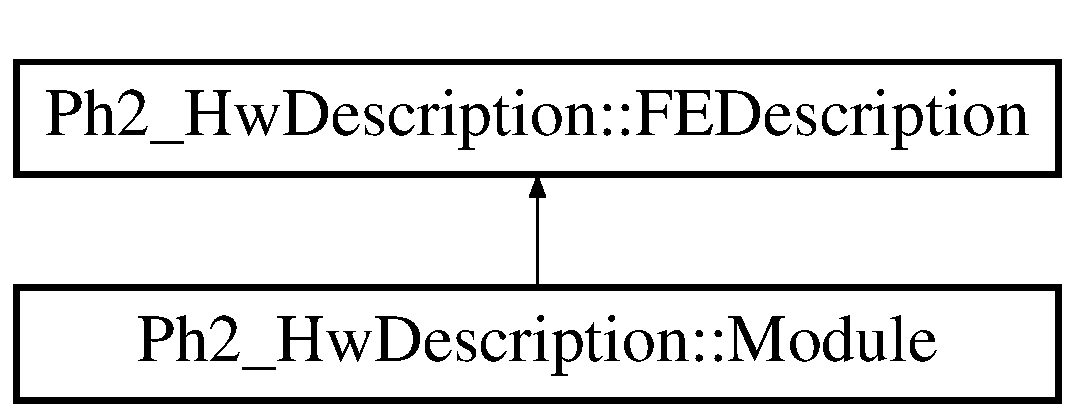
\includegraphics[height=2.000000cm]{class_ph2___hw_description_1_1_module}
\end{center}
\end{figure}
\subsection*{Public Member Functions}
\begin{DoxyCompactItemize}
\item 
\hyperlink{class_ph2___hw_description_1_1_module_adab1cde05b3a83e7199f5b55166074ed}{Module} (\hyperlink{class_ph2___hw_description_1_1_front_end_description}{Front\-End\-Description} \&p\-Fe\-Desc)
\item 
\hyperlink{class_ph2___hw_description_1_1_module_acb5e5f17c946438f985c209563060f26}{Module} (uint8\-\_\-t p\-Shelve\-Id, uint8\-\_\-t p\-Be\-Id, uint8\-\_\-t p\-F\-M\-C\-Id, uint8\-\_\-t p\-Fe\-Id, uint8\-\_\-t p\-Module\-Id)
\item 
\hyperlink{class_ph2___hw_description_1_1_module_aaec7dd439bdf7a1db3f2136569a00125}{Module} ()
\item 
\hyperlink{class_ph2___hw_description_1_1_module_a8142f34ea2308ed78e8d0dbb042bc5f3}{$\sim$\-Module} ()
\item 
uint8\-\_\-t \hyperlink{class_ph2___hw_description_1_1_module_a8703442b1055c0c38b4157fc155ac084}{get\-N\-Cbc} ()
\begin{DoxyCompactList}\small\item\em Get the number of \hyperlink{class_ph2___hw_description_1_1_cbc}{Cbc} connected to the \hyperlink{class_ph2___hw_description_1_1_module}{Module}. \end{DoxyCompactList}\item 
void \hyperlink{class_ph2___hw_description_1_1_module_ac2743d5056bc3053bf472e5fd94bbf14}{add\-Cbc} (\hyperlink{class_ph2___hw_description_1_1_cbc}{Cbc} \&p\-Cbc)
\begin{DoxyCompactList}\small\item\em Adding a \hyperlink{class_ph2___hw_description_1_1_cbc}{Cbc} to the vector. \end{DoxyCompactList}\item 
bool \hyperlink{class_ph2___hw_description_1_1_module_a0aa7c940311bd13a32fd4e0f251c2d27}{remove\-Cbc} (uint8\-\_\-t p\-Cbc\-Id)
\begin{DoxyCompactList}\small\item\em Remove a \hyperlink{class_ph2___hw_description_1_1_cbc}{Cbc} from the vector. \end{DoxyCompactList}\item 
\hyperlink{class_ph2___hw_description_1_1_cbc}{Cbc} $\ast$ \hyperlink{class_ph2___hw_description_1_1_module_a05ccbee9ca3eb8022e359b5e9dabe783}{get\-Cbc} (uint8\-\_\-t p\-Cbc\-Id)
\begin{DoxyCompactList}\small\item\em Get a \hyperlink{class_ph2___hw_description_1_1_cbc}{Cbc} from the vector. \end{DoxyCompactList}\end{DoxyCompactItemize}
\subsection*{Data Fields}
\begin{DoxyCompactItemize}
\item 
uint8\-\_\-t \hyperlink{class_ph2___hw_description_1_1_module_a8bf42ae708d304acbc5509edf7f7cee0}{f\-Module\-Id}
\end{DoxyCompactItemize}
\subsection*{Protected Attributes}
\begin{DoxyCompactItemize}
\item 
std\-::vector$<$ \hyperlink{class_ph2___hw_description_1_1_cbc}{Cbc} $>$ \hyperlink{class_ph2___hw_description_1_1_module_ab5cfd93bf927592f609d31f66cd4161b}{f\-Cbc\-Vector}
\end{DoxyCompactItemize}


\subsection{Detailed Description}
contains a vector of \hyperlink{class_ph2___hw_description_1_1_cbc}{Cbc} which are connected to the \hyperlink{class_ph2___hw_description_1_1_module}{Module} 

\subsection{Constructor \& Destructor Documentation}
\hypertarget{class_ph2___hw_description_1_1_module_adab1cde05b3a83e7199f5b55166074ed}{\index{Ph2\-\_\-\-Hw\-Description\-::\-Module@{Ph2\-\_\-\-Hw\-Description\-::\-Module}!Module@{Module}}
\index{Module@{Module}!Ph2_HwDescription::Module@{Ph2\-\_\-\-Hw\-Description\-::\-Module}}
\subsubsection[{Module}]{\setlength{\rightskip}{0pt plus 5cm}Ph2\-\_\-\-Hw\-Description\-::\-Module\-::\-Module (
\begin{DoxyParamCaption}
\item[{{\bf Front\-End\-Description} \&}]{p\-Fe\-Desc}
\end{DoxyParamCaption}
)}}\label{class_ph2___hw_description_1_1_module_adab1cde05b3a83e7199f5b55166074ed}
\hypertarget{class_ph2___hw_description_1_1_module_acb5e5f17c946438f985c209563060f26}{\index{Ph2\-\_\-\-Hw\-Description\-::\-Module@{Ph2\-\_\-\-Hw\-Description\-::\-Module}!Module@{Module}}
\index{Module@{Module}!Ph2_HwDescription::Module@{Ph2\-\_\-\-Hw\-Description\-::\-Module}}
\subsubsection[{Module}]{\setlength{\rightskip}{0pt plus 5cm}Ph2\-\_\-\-Hw\-Description\-::\-Module\-::\-Module (
\begin{DoxyParamCaption}
\item[{uint8\-\_\-t}]{p\-Shelve\-Id, }
\item[{uint8\-\_\-t}]{p\-Be\-Id, }
\item[{uint8\-\_\-t}]{p\-F\-M\-C\-Id, }
\item[{uint8\-\_\-t}]{p\-Fe\-Id, }
\item[{uint8\-\_\-t}]{p\-Module\-Id}
\end{DoxyParamCaption}
)}}\label{class_ph2___hw_description_1_1_module_acb5e5f17c946438f985c209563060f26}
\hypertarget{class_ph2___hw_description_1_1_module_aaec7dd439bdf7a1db3f2136569a00125}{\index{Ph2\-\_\-\-Hw\-Description\-::\-Module@{Ph2\-\_\-\-Hw\-Description\-::\-Module}!Module@{Module}}
\index{Module@{Module}!Ph2_HwDescription::Module@{Ph2\-\_\-\-Hw\-Description\-::\-Module}}
\subsubsection[{Module}]{\setlength{\rightskip}{0pt plus 5cm}Ph2\-\_\-\-Hw\-Description\-::\-Module\-::\-Module (
\begin{DoxyParamCaption}
{}
\end{DoxyParamCaption}
)}}\label{class_ph2___hw_description_1_1_module_aaec7dd439bdf7a1db3f2136569a00125}
\hypertarget{class_ph2___hw_description_1_1_module_a8142f34ea2308ed78e8d0dbb042bc5f3}{\index{Ph2\-\_\-\-Hw\-Description\-::\-Module@{Ph2\-\_\-\-Hw\-Description\-::\-Module}!$\sim$\-Module@{$\sim$\-Module}}
\index{$\sim$\-Module@{$\sim$\-Module}!Ph2_HwDescription::Module@{Ph2\-\_\-\-Hw\-Description\-::\-Module}}
\subsubsection[{$\sim$\-Module}]{\setlength{\rightskip}{0pt plus 5cm}Ph2\-\_\-\-Hw\-Description\-::\-Module\-::$\sim$\-Module (
\begin{DoxyParamCaption}
{}
\end{DoxyParamCaption}
)\hspace{0.3cm}{\ttfamily [inline]}}}\label{class_ph2___hw_description_1_1_module_a8142f34ea2308ed78e8d0dbb042bc5f3}


\subsection{Member Function Documentation}
\hypertarget{class_ph2___hw_description_1_1_module_ac2743d5056bc3053bf472e5fd94bbf14}{\index{Ph2\-\_\-\-Hw\-Description\-::\-Module@{Ph2\-\_\-\-Hw\-Description\-::\-Module}!add\-Cbc@{add\-Cbc}}
\index{add\-Cbc@{add\-Cbc}!Ph2_HwDescription::Module@{Ph2\-\_\-\-Hw\-Description\-::\-Module}}
\subsubsection[{add\-Cbc}]{\setlength{\rightskip}{0pt plus 5cm}void Ph2\-\_\-\-Hw\-Description\-::\-Module\-::add\-Cbc (
\begin{DoxyParamCaption}
\item[{{\bf Cbc} \&}]{p\-Cbc}
\end{DoxyParamCaption}
)}}\label{class_ph2___hw_description_1_1_module_ac2743d5056bc3053bf472e5fd94bbf14}


Adding a \hyperlink{class_ph2___hw_description_1_1_cbc}{Cbc} to the vector. 


\begin{DoxyParams}{Parameters}
{\em p\-Cbc} & \\
\hline
\end{DoxyParams}
\hypertarget{class_ph2___hw_description_1_1_module_a05ccbee9ca3eb8022e359b5e9dabe783}{\index{Ph2\-\_\-\-Hw\-Description\-::\-Module@{Ph2\-\_\-\-Hw\-Description\-::\-Module}!get\-Cbc@{get\-Cbc}}
\index{get\-Cbc@{get\-Cbc}!Ph2_HwDescription::Module@{Ph2\-\_\-\-Hw\-Description\-::\-Module}}
\subsubsection[{get\-Cbc}]{\setlength{\rightskip}{0pt plus 5cm}{\bf Cbc} $\ast$ Ph2\-\_\-\-Hw\-Description\-::\-Module\-::get\-Cbc (
\begin{DoxyParamCaption}
\item[{uint8\-\_\-t}]{p\-Cbc\-Id}
\end{DoxyParamCaption}
)}}\label{class_ph2___hw_description_1_1_module_a05ccbee9ca3eb8022e359b5e9dabe783}


Get a \hyperlink{class_ph2___hw_description_1_1_cbc}{Cbc} from the vector. 


\begin{DoxyParams}{Parameters}
{\em p\-Cbc\-Id} & \\
\hline
\end{DoxyParams}
\begin{DoxyReturn}{Returns}
a pointer of \hyperlink{class_ph2___hw_description_1_1_cbc}{Cbc}, so we can manipulate directly the \hyperlink{class_ph2___hw_description_1_1_cbc}{Cbc} contained in the vector 
\end{DoxyReturn}
\hypertarget{class_ph2___hw_description_1_1_module_a8703442b1055c0c38b4157fc155ac084}{\index{Ph2\-\_\-\-Hw\-Description\-::\-Module@{Ph2\-\_\-\-Hw\-Description\-::\-Module}!get\-N\-Cbc@{get\-N\-Cbc}}
\index{get\-N\-Cbc@{get\-N\-Cbc}!Ph2_HwDescription::Module@{Ph2\-\_\-\-Hw\-Description\-::\-Module}}
\subsubsection[{get\-N\-Cbc}]{\setlength{\rightskip}{0pt plus 5cm}uint8\-\_\-t Ph2\-\_\-\-Hw\-Description\-::\-Module\-::get\-N\-Cbc (
\begin{DoxyParamCaption}
{}
\end{DoxyParamCaption}
)\hspace{0.3cm}{\ttfamily [inline]}}}\label{class_ph2___hw_description_1_1_module_a8703442b1055c0c38b4157fc155ac084}


Get the number of \hyperlink{class_ph2___hw_description_1_1_cbc}{Cbc} connected to the \hyperlink{class_ph2___hw_description_1_1_module}{Module}. 

\begin{DoxyReturn}{Returns}
The size of the vector 
\end{DoxyReturn}
\hypertarget{class_ph2___hw_description_1_1_module_a0aa7c940311bd13a32fd4e0f251c2d27}{\index{Ph2\-\_\-\-Hw\-Description\-::\-Module@{Ph2\-\_\-\-Hw\-Description\-::\-Module}!remove\-Cbc@{remove\-Cbc}}
\index{remove\-Cbc@{remove\-Cbc}!Ph2_HwDescription::Module@{Ph2\-\_\-\-Hw\-Description\-::\-Module}}
\subsubsection[{remove\-Cbc}]{\setlength{\rightskip}{0pt plus 5cm}bool Ph2\-\_\-\-Hw\-Description\-::\-Module\-::remove\-Cbc (
\begin{DoxyParamCaption}
\item[{uint8\-\_\-t}]{p\-Cbc\-Id}
\end{DoxyParamCaption}
)}}\label{class_ph2___hw_description_1_1_module_a0aa7c940311bd13a32fd4e0f251c2d27}


Remove a \hyperlink{class_ph2___hw_description_1_1_cbc}{Cbc} from the vector. 


\begin{DoxyParams}{Parameters}
{\em p\-Cbc\-Id} & \\
\hline
\end{DoxyParams}
\begin{DoxyReturn}{Returns}
a bool which indicate if the removing was successful 
\end{DoxyReturn}


\subsection{Field Documentation}
\hypertarget{class_ph2___hw_description_1_1_module_ab5cfd93bf927592f609d31f66cd4161b}{\index{Ph2\-\_\-\-Hw\-Description\-::\-Module@{Ph2\-\_\-\-Hw\-Description\-::\-Module}!f\-Cbc\-Vector@{f\-Cbc\-Vector}}
\index{f\-Cbc\-Vector@{f\-Cbc\-Vector}!Ph2_HwDescription::Module@{Ph2\-\_\-\-Hw\-Description\-::\-Module}}
\subsubsection[{f\-Cbc\-Vector}]{\setlength{\rightskip}{0pt plus 5cm}std\-::vector$<$ {\bf Cbc} $>$ Ph2\-\_\-\-Hw\-Description\-::\-Module\-::f\-Cbc\-Vector\hspace{0.3cm}{\ttfamily [protected]}}}\label{class_ph2___hw_description_1_1_module_ab5cfd93bf927592f609d31f66cd4161b}
\hypertarget{class_ph2___hw_description_1_1_module_a8bf42ae708d304acbc5509edf7f7cee0}{\index{Ph2\-\_\-\-Hw\-Description\-::\-Module@{Ph2\-\_\-\-Hw\-Description\-::\-Module}!f\-Module\-Id@{f\-Module\-Id}}
\index{f\-Module\-Id@{f\-Module\-Id}!Ph2_HwDescription::Module@{Ph2\-\_\-\-Hw\-Description\-::\-Module}}
\subsubsection[{f\-Module\-Id}]{\setlength{\rightskip}{0pt plus 5cm}uint8\-\_\-t Ph2\-\_\-\-Hw\-Description\-::\-Module\-::f\-Module\-Id}}\label{class_ph2___hw_description_1_1_module_a8bf42ae708d304acbc5509edf7f7cee0}


The documentation for this class was generated from the following files\-:\begin{DoxyCompactItemize}
\item 
H\-W\-Description/\hyperlink{_module_8h}{Module.\-h}\item 
H\-W\-Description/\hyperlink{_module_8cc}{Module.\-cc}\end{DoxyCompactItemize}

\hypertarget{structnamespace__uri__predicate}{\section{namespace\-\_\-uri\-\_\-predicate Struct Reference}
\label{structnamespace__uri__predicate}\index{namespace\-\_\-uri\-\_\-predicate@{namespace\-\_\-uri\-\_\-predicate}}
}
\subsection*{Public Member Functions}
\begin{DoxyCompactItemize}
\item 
\hyperlink{structnamespace__uri__predicate_a25bef9c1e12b0fdc908275ae7ab7c202}{namespace\-\_\-uri\-\_\-predicate} (const char\-\_\-t $\ast$name)
\item 
bool \hyperlink{structnamespace__uri__predicate_ab4580e45d603d3eedfe75fec74210ce1}{operator()} (const xml\-\_\-attribute \&a) const 
\end{DoxyCompactItemize}
\subsection*{Data Fields}
\begin{DoxyCompactItemize}
\item 
const char\-\_\-t $\ast$ \hyperlink{structnamespace__uri__predicate_a80a2c051b9e57b8895c28d8fcc32e051}{prefix}
\item 
size\-\_\-t \hyperlink{structnamespace__uri__predicate_aa48279192e8d48b9c798f5485a2a9170}{prefix\-\_\-length}
\end{DoxyCompactItemize}


\subsection{Constructor \& Destructor Documentation}
\hypertarget{structnamespace__uri__predicate_a25bef9c1e12b0fdc908275ae7ab7c202}{\index{namespace\-\_\-uri\-\_\-predicate@{namespace\-\_\-uri\-\_\-predicate}!namespace\-\_\-uri\-\_\-predicate@{namespace\-\_\-uri\-\_\-predicate}}
\index{namespace\-\_\-uri\-\_\-predicate@{namespace\-\_\-uri\-\_\-predicate}!namespace_uri_predicate@{namespace\-\_\-uri\-\_\-predicate}}
\subsubsection[{namespace\-\_\-uri\-\_\-predicate}]{\setlength{\rightskip}{0pt plus 5cm}namespace\-\_\-uri\-\_\-predicate\-::namespace\-\_\-uri\-\_\-predicate (
\begin{DoxyParamCaption}
\item[{const char\-\_\-t $\ast$}]{name}
\end{DoxyParamCaption}
)\hspace{0.3cm}{\ttfamily [inline]}}}\label{structnamespace__uri__predicate_a25bef9c1e12b0fdc908275ae7ab7c202}


\subsection{Member Function Documentation}
\hypertarget{structnamespace__uri__predicate_ab4580e45d603d3eedfe75fec74210ce1}{\index{namespace\-\_\-uri\-\_\-predicate@{namespace\-\_\-uri\-\_\-predicate}!operator()@{operator()}}
\index{operator()@{operator()}!namespace_uri_predicate@{namespace\-\_\-uri\-\_\-predicate}}
\subsubsection[{operator()}]{\setlength{\rightskip}{0pt plus 5cm}bool namespace\-\_\-uri\-\_\-predicate\-::operator() (
\begin{DoxyParamCaption}
\item[{const xml\-\_\-attribute \&}]{a}
\end{DoxyParamCaption}
) const\hspace{0.3cm}{\ttfamily [inline]}}}\label{structnamespace__uri__predicate_ab4580e45d603d3eedfe75fec74210ce1}


\subsection{Field Documentation}
\hypertarget{structnamespace__uri__predicate_a80a2c051b9e57b8895c28d8fcc32e051}{\index{namespace\-\_\-uri\-\_\-predicate@{namespace\-\_\-uri\-\_\-predicate}!prefix@{prefix}}
\index{prefix@{prefix}!namespace_uri_predicate@{namespace\-\_\-uri\-\_\-predicate}}
\subsubsection[{prefix}]{\setlength{\rightskip}{0pt plus 5cm}const char\-\_\-t$\ast$ namespace\-\_\-uri\-\_\-predicate\-::prefix}}\label{structnamespace__uri__predicate_a80a2c051b9e57b8895c28d8fcc32e051}
\hypertarget{structnamespace__uri__predicate_aa48279192e8d48b9c798f5485a2a9170}{\index{namespace\-\_\-uri\-\_\-predicate@{namespace\-\_\-uri\-\_\-predicate}!prefix\-\_\-length@{prefix\-\_\-length}}
\index{prefix\-\_\-length@{prefix\-\_\-length}!namespace_uri_predicate@{namespace\-\_\-uri\-\_\-predicate}}
\subsubsection[{prefix\-\_\-length}]{\setlength{\rightskip}{0pt plus 5cm}size\-\_\-t namespace\-\_\-uri\-\_\-predicate\-::prefix\-\_\-length}}\label{structnamespace__uri__predicate_aa48279192e8d48b9c798f5485a2a9170}


The documentation for this struct was generated from the following file\-:\begin{DoxyCompactItemize}
\item 
System/\hyperlink{pugixml_8cpp}{pugixml.\-cpp}\end{DoxyCompactItemize}

\hypertarget{structnot__equal__to}{\section{not\-\_\-equal\-\_\-to Struct Reference}
\label{structnot__equal__to}\index{not\-\_\-equal\-\_\-to@{not\-\_\-equal\-\_\-to}}
}
\subsection*{Public Member Functions}
\begin{DoxyCompactItemize}
\item 
{\footnotesize template$<$typename T $>$ }\\bool \hyperlink{structnot__equal__to_acbcb7d0809378458b52e6ed1a07c1d7d}{operator()} (const T \&lhs, const T \&rhs) const 
\end{DoxyCompactItemize}


\subsection{Member Function Documentation}
\hypertarget{structnot__equal__to_acbcb7d0809378458b52e6ed1a07c1d7d}{\index{not\-\_\-equal\-\_\-to@{not\-\_\-equal\-\_\-to}!operator()@{operator()}}
\index{operator()@{operator()}!not_equal_to@{not\-\_\-equal\-\_\-to}}
\subsubsection[{operator()}]{\setlength{\rightskip}{0pt plus 5cm}template$<$typename T $>$ bool not\-\_\-equal\-\_\-to\-::operator() (
\begin{DoxyParamCaption}
\item[{const T \&}]{lhs, }
\item[{const T \&}]{rhs}
\end{DoxyParamCaption}
) const\hspace{0.3cm}{\ttfamily [inline]}}}\label{structnot__equal__to_acbcb7d0809378458b52e6ed1a07c1d7d}


The documentation for this struct was generated from the following file\-:\begin{DoxyCompactItemize}
\item 
System/\hyperlink{pugixml_8cpp}{pugixml.\-cpp}\end{DoxyCompactItemize}

\hypertarget{structopt__false}{\section{opt\-\_\-false Struct Reference}
\label{structopt__false}\index{opt\-\_\-false@{opt\-\_\-false}}
}
\subsection*{Public Types}
\begin{DoxyCompactItemize}
\item 
enum \{ \hyperlink{structopt__false_adf1eb3ad7c3e284bd861d80d6817174fa0608b30b4b0f63ec3263f29fe847899e}{value} = 0
 \}
\end{DoxyCompactItemize}


\subsection{Member Enumeration Documentation}
\hypertarget{structopt__false_adf1eb3ad7c3e284bd861d80d6817174f}{\subsubsection[{anonymous enum}]{\setlength{\rightskip}{0pt plus 5cm}anonymous enum}}\label{structopt__false_adf1eb3ad7c3e284bd861d80d6817174f}
\begin{Desc}
\item[Enumerator]\par
\begin{description}
\index{value@{value}!opt\-\_\-false@{opt\-\_\-false}}\index{opt\-\_\-false@{opt\-\_\-false}!value@{value}}\item[{\em 
\hypertarget{structopt__false_adf1eb3ad7c3e284bd861d80d6817174fa0608b30b4b0f63ec3263f29fe847899e}{value}\label{structopt__false_adf1eb3ad7c3e284bd861d80d6817174fa0608b30b4b0f63ec3263f29fe847899e}
}]\end{description}
\end{Desc}


The documentation for this struct was generated from the following file\-:\begin{DoxyCompactItemize}
\item 
System/\hyperlink{pugixml_8cpp}{pugixml.\-cpp}\end{DoxyCompactItemize}

\hypertarget{structopt__true}{
\section{opt\_\-true Struct Reference}
\label{structopt__true}\index{opt_true@{opt\_\-true}}
}
\subsection*{Public Types}
\begin{CompactItemize}
\item 
\hyperlink{structopt__true_6b3a9dd06e76271df50cfd55f92fffc23f8405655cc98a5710236f177e042b72}{value} = 1
\item 
enum \{ \hyperlink{structopt__true_6b3a9dd06e76271df50cfd55f92fffc23f8405655cc98a5710236f177e042b72}{value} =  1
 \}
\end{CompactItemize}


\subsection{Member Enumeration Documentation}
\hypertarget{structopt__true_6b3a9dd06e76271df50cfd55f92fffc2}{
\subsubsection["@3]{\setlength{\rightskip}{0pt plus 5cm}anonymous enum}}
\label{structopt__true_6b3a9dd06e76271df50cfd55f92fffc2}


\begin{Desc}
\item[Enumerator: ]\par
\begin{description}
\index{value@{value}!opt_true@{opt\_\-true}}\index{opt_true@{opt\_\-true}!value@{value}}\item[{\em 
\hypertarget{structopt__true_6b3a9dd06e76271df50cfd55f92fffc23f8405655cc98a5710236f177e042b72}{
value}
\label{structopt__true_6b3a9dd06e76271df50cfd55f92fffc23f8405655cc98a5710236f177e042b72}
}]\end{description}
\end{Desc}



The documentation for this struct was generated from the following file:\begin{CompactItemize}
\item 
Utils/\hyperlink{pugixml_8cpp}{pugixml.cpp}\end{CompactItemize}

\hypertarget{struct_ph2___hw_description_1_1_reg_item_comparer}{\section{Ph2\-\_\-\-Hw\-Description\-:\-:Reg\-Item\-Comparer Struct Reference}
\label{struct_ph2___hw_description_1_1_reg_item_comparer}\index{Ph2\-\_\-\-Hw\-Description\-::\-Reg\-Item\-Comparer@{Ph2\-\_\-\-Hw\-Description\-::\-Reg\-Item\-Comparer}}
}


Compare two pair of Register Name Versus \hyperlink{struct_ph2___hw_description_1_1_cbc_reg_item}{Cbc\-Reg\-Item} by the Page and Adress of the \hyperlink{struct_ph2___hw_description_1_1_cbc_reg_item}{Cbc\-Reg\-Item}.  




{\ttfamily \#include $<$Cbc.\-h$>$}

\subsection*{Public Member Functions}
\begin{DoxyCompactItemize}
\item 
bool \hyperlink{struct_ph2___hw_description_1_1_reg_item_comparer_aee3e1f2a92ae7431674b6307478c8c6f}{operator()} (\hyperlink{namespace_ph2___hw_description_a78856413327152e693dceca249188d11}{Cbc\-Reg\-Pair} p\-Reg\-Item1, \hyperlink{namespace_ph2___hw_description_a78856413327152e693dceca249188d11}{Cbc\-Reg\-Pair} p\-Reg\-Item2)
\end{DoxyCompactItemize}


\subsection{Detailed Description}
Compare two pair of Register Name Versus \hyperlink{struct_ph2___hw_description_1_1_cbc_reg_item}{Cbc\-Reg\-Item} by the Page and Adress of the \hyperlink{struct_ph2___hw_description_1_1_cbc_reg_item}{Cbc\-Reg\-Item}. 

\subsection{Member Function Documentation}
\hypertarget{struct_ph2___hw_description_1_1_reg_item_comparer_aee3e1f2a92ae7431674b6307478c8c6f}{\index{Ph2\-\_\-\-Hw\-Description\-::\-Reg\-Item\-Comparer@{Ph2\-\_\-\-Hw\-Description\-::\-Reg\-Item\-Comparer}!operator()@{operator()}}
\index{operator()@{operator()}!Ph2_HwDescription::RegItemComparer@{Ph2\-\_\-\-Hw\-Description\-::\-Reg\-Item\-Comparer}}
\subsubsection[{operator()}]{\setlength{\rightskip}{0pt plus 5cm}bool Ph2\-\_\-\-Hw\-Description\-::\-Reg\-Item\-Comparer\-::operator() (
\begin{DoxyParamCaption}
\item[{{\bf Cbc\-Reg\-Pair}}]{p\-Reg\-Item1, }
\item[{{\bf Cbc\-Reg\-Pair}}]{p\-Reg\-Item2}
\end{DoxyParamCaption}
)}}\label{struct_ph2___hw_description_1_1_reg_item_comparer_aee3e1f2a92ae7431674b6307478c8c6f}


The documentation for this struct was generated from the following files\-:\begin{DoxyCompactItemize}
\item 
H\-W\-Description/\hyperlink{_cbc_8h}{Cbc.\-h}\item 
H\-W\-Description/\hyperlink{_cbc_8cc}{Cbc.\-cc}\end{DoxyCompactItemize}

\hypertarget{class_ph2___hw_interface_1_1_reg_manager}{\section{Ph2\-\_\-\-Hw\-Interface\-:\-:Reg\-Manager Class Reference}
\label{class_ph2___hw_interface_1_1_reg_manager}\index{Ph2\-\_\-\-Hw\-Interface\-::\-Reg\-Manager@{Ph2\-\_\-\-Hw\-Interface\-::\-Reg\-Manager}}
}


Permit connection to given boards and r/w given registers.  




{\ttfamily \#include $<$Reg\-Manager.\-h$>$}

Inheritance diagram for Ph2\-\_\-\-Hw\-Interface\-:\-:Reg\-Manager\-:\begin{figure}[H]
\begin{center}
\leavevmode
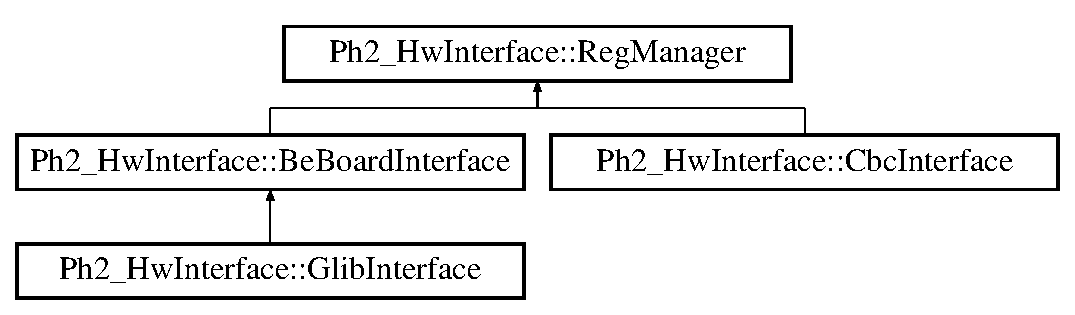
\includegraphics[height=2.000000cm]{class_ph2___hw_interface_1_1_reg_manager}
\end{center}
\end{figure}
\subsection*{Public Member Functions}
\begin{DoxyCompactItemize}
\item 
\hyperlink{class_ph2___hw_interface_1_1_reg_manager_a938f6b582b1fffcb478f35fd9d81954f}{Reg\-Manager} (const char $\ast$pu\-Hal\-Config\-File\-Name)
\begin{DoxyCompactList}\small\item\em Constructor of the \hyperlink{class_ph2___hw_interface_1_1_reg_manager}{Reg\-Manager} class. \end{DoxyCompactList}\item 
virtual \hyperlink{class_ph2___hw_interface_1_1_reg_manager_a5d650c4e6467153f98f999abbbfc354c}{$\sim$\-Reg\-Manager} ()
\begin{DoxyCompactList}\small\item\em Destructor of the \hyperlink{class_ph2___hw_interface_1_1_reg_manager}{Reg\-Manager} class. \end{DoxyCompactList}\end{DoxyCompactItemize}
\subsection*{Protected Member Functions}
\begin{DoxyCompactItemize}
\item 
virtual bool \hyperlink{class_ph2___hw_interface_1_1_reg_manager_a31174516fef6706c88c3f59dd93e4fdf}{Write\-Reg} (const std\-::string \&p\-Reg\-Node, const uint32\-\_\-t \&p\-Val)
\begin{DoxyCompactList}\small\item\em Write a register. \end{DoxyCompactList}\item 
virtual bool \hyperlink{class_ph2___hw_interface_1_1_reg_manager_a888f5cccb05daa28896cf622abfdcbd6}{Write\-Block\-Reg} (const std\-::string \&p\-Reg\-Node, const std\-::vector$<$ uint32\-\_\-t $>$ \&p\-Values)
\begin{DoxyCompactList}\small\item\em Write a block of values in a register. \end{DoxyCompactList}\item 
virtual uhal\-::\-Val\-Word$<$ uint32\-\_\-t $>$ \hyperlink{class_ph2___hw_interface_1_1_reg_manager_a077e0a18592206365150680213345112}{Read\-Reg} (const std\-::string \&p\-Reg\-Node)
\begin{DoxyCompactList}\small\item\em Read a value in a register. \end{DoxyCompactList}\item 
virtual uhal\-::\-Val\-Vector$<$ uint32\-\_\-t $>$ \hyperlink{class_ph2___hw_interface_1_1_reg_manager_a6481c211d27badc409ff0e7af20575e4}{Read\-Block\-Reg} (const std\-::string \&p\-Reg\-Node, const uint32\-\_\-t \&p\-Blocksize)
\begin{DoxyCompactList}\small\item\em Read a block of values in a register. \end{DoxyCompactList}\item 
virtual void \hyperlink{class_ph2___hw_interface_1_1_reg_manager_a20c502bcad5115c6ae16d4d356b72f0c}{Choose\-Board} (uint8\-\_\-t p\-Board\-Id)
\begin{DoxyCompactList}\small\item\em Choose the board we want to talk with. \end{DoxyCompactList}\end{DoxyCompactItemize}
\subsection*{Protected Attributes}
\begin{DoxyCompactItemize}
\item 
uhal\-::\-Hw\-Interface $\ast$ \hyperlink{class_ph2___hw_interface_1_1_reg_manager_a0d4908ec834a3a0b7d8139872fd0a4a0}{f\-Board}
\item 
const char $\ast$ \hyperlink{class_ph2___hw_interface_1_1_reg_manager_aaaa29ca65c283acc645132c7bef0f24f}{f\-U\-Hal\-Config\-File\-Name}
\item 
std\-::map$<$ uint8\-\_\-t, \\*
uhal\-::\-Hw\-Interface $\ast$ $>$ \hyperlink{class_ph2___hw_interface_1_1_reg_manager_a9c34ffe467a572796c05036533bb6d39}{f\-Board\-Map}
\end{DoxyCompactItemize}


\subsection{Detailed Description}
Permit connection to given boards and r/w given registers. 

\subsection{Constructor \& Destructor Documentation}
\hypertarget{class_ph2___hw_interface_1_1_reg_manager_a938f6b582b1fffcb478f35fd9d81954f}{\index{Ph2\-\_\-\-Hw\-Interface\-::\-Reg\-Manager@{Ph2\-\_\-\-Hw\-Interface\-::\-Reg\-Manager}!Reg\-Manager@{Reg\-Manager}}
\index{Reg\-Manager@{Reg\-Manager}!Ph2_HwInterface::RegManager@{Ph2\-\_\-\-Hw\-Interface\-::\-Reg\-Manager}}
\subsubsection[{Reg\-Manager}]{\setlength{\rightskip}{0pt plus 5cm}Ph2\-\_\-\-Hw\-Interface\-::\-Reg\-Manager\-::\-Reg\-Manager (
\begin{DoxyParamCaption}
\item[{const char $\ast$}]{pu\-Hal\-Config\-File\-Name}
\end{DoxyParamCaption}
)}}\label{class_ph2___hw_interface_1_1_reg_manager_a938f6b582b1fffcb478f35fd9d81954f}


Constructor of the \hyperlink{class_ph2___hw_interface_1_1_reg_manager}{Reg\-Manager} class. 


\begin{DoxyParams}{Parameters}
{\em pu\-Hal\-Config\-File\-Name} & \-: path of the u\-Hal Config File \\
\hline
\end{DoxyParams}
\hypertarget{class_ph2___hw_interface_1_1_reg_manager_a5d650c4e6467153f98f999abbbfc354c}{\index{Ph2\-\_\-\-Hw\-Interface\-::\-Reg\-Manager@{Ph2\-\_\-\-Hw\-Interface\-::\-Reg\-Manager}!$\sim$\-Reg\-Manager@{$\sim$\-Reg\-Manager}}
\index{$\sim$\-Reg\-Manager@{$\sim$\-Reg\-Manager}!Ph2_HwInterface::RegManager@{Ph2\-\_\-\-Hw\-Interface\-::\-Reg\-Manager}}
\subsubsection[{$\sim$\-Reg\-Manager}]{\setlength{\rightskip}{0pt plus 5cm}Ph2\-\_\-\-Hw\-Interface\-::\-Reg\-Manager\-::$\sim$\-Reg\-Manager (
\begin{DoxyParamCaption}
{}
\end{DoxyParamCaption}
)\hspace{0.3cm}{\ttfamily [virtual]}}}\label{class_ph2___hw_interface_1_1_reg_manager_a5d650c4e6467153f98f999abbbfc354c}


Destructor of the \hyperlink{class_ph2___hw_interface_1_1_reg_manager}{Reg\-Manager} class. 



\subsection{Member Function Documentation}
\hypertarget{class_ph2___hw_interface_1_1_reg_manager_a20c502bcad5115c6ae16d4d356b72f0c}{\index{Ph2\-\_\-\-Hw\-Interface\-::\-Reg\-Manager@{Ph2\-\_\-\-Hw\-Interface\-::\-Reg\-Manager}!Choose\-Board@{Choose\-Board}}
\index{Choose\-Board@{Choose\-Board}!Ph2_HwInterface::RegManager@{Ph2\-\_\-\-Hw\-Interface\-::\-Reg\-Manager}}
\subsubsection[{Choose\-Board}]{\setlength{\rightskip}{0pt plus 5cm}void Ph2\-\_\-\-Hw\-Interface\-::\-Reg\-Manager\-::\-Choose\-Board (
\begin{DoxyParamCaption}
\item[{uint8\-\_\-t}]{p\-Board\-Id}
\end{DoxyParamCaption}
)\hspace{0.3cm}{\ttfamily [protected]}, {\ttfamily [virtual]}}}\label{class_ph2___hw_interface_1_1_reg_manager_a20c502bcad5115c6ae16d4d356b72f0c}


Choose the board we want to talk with. 


\begin{DoxyParams}{Parameters}
{\em p\-Board\-Id} & \-: Id of the Board to connect to \\
\hline
\end{DoxyParams}
\hypertarget{class_ph2___hw_interface_1_1_reg_manager_a6481c211d27badc409ff0e7af20575e4}{\index{Ph2\-\_\-\-Hw\-Interface\-::\-Reg\-Manager@{Ph2\-\_\-\-Hw\-Interface\-::\-Reg\-Manager}!Read\-Block\-Reg@{Read\-Block\-Reg}}
\index{Read\-Block\-Reg@{Read\-Block\-Reg}!Ph2_HwInterface::RegManager@{Ph2\-\_\-\-Hw\-Interface\-::\-Reg\-Manager}}
\subsubsection[{Read\-Block\-Reg}]{\setlength{\rightskip}{0pt plus 5cm}uhal\-::\-Val\-Vector$<$ uint32\-\_\-t $>$ Ph2\-\_\-\-Hw\-Interface\-::\-Reg\-Manager\-::\-Read\-Block\-Reg (
\begin{DoxyParamCaption}
\item[{const std\-::string \&}]{p\-Reg\-Node, }
\item[{const uint32\-\_\-t \&}]{p\-Blocksize}
\end{DoxyParamCaption}
)\hspace{0.3cm}{\ttfamily [protected]}, {\ttfamily [virtual]}}}\label{class_ph2___hw_interface_1_1_reg_manager_a6481c211d27badc409ff0e7af20575e4}


Read a block of values in a register. 


\begin{DoxyParams}{Parameters}
{\em p\-Reg\-Node} & \-: Node of the register to read \\
\hline
{\em p\-Blocksize} & \-: Size of the block to read \\
\hline
\end{DoxyParams}
\begin{DoxyReturn}{Returns}
Val\-Vector block values of the register 
\end{DoxyReturn}
\hypertarget{class_ph2___hw_interface_1_1_reg_manager_a077e0a18592206365150680213345112}{\index{Ph2\-\_\-\-Hw\-Interface\-::\-Reg\-Manager@{Ph2\-\_\-\-Hw\-Interface\-::\-Reg\-Manager}!Read\-Reg@{Read\-Reg}}
\index{Read\-Reg@{Read\-Reg}!Ph2_HwInterface::RegManager@{Ph2\-\_\-\-Hw\-Interface\-::\-Reg\-Manager}}
\subsubsection[{Read\-Reg}]{\setlength{\rightskip}{0pt plus 5cm}uhal\-::\-Val\-Word$<$ uint32\-\_\-t $>$ Ph2\-\_\-\-Hw\-Interface\-::\-Reg\-Manager\-::\-Read\-Reg (
\begin{DoxyParamCaption}
\item[{const std\-::string \&}]{p\-Reg\-Node}
\end{DoxyParamCaption}
)\hspace{0.3cm}{\ttfamily [protected]}, {\ttfamily [virtual]}}}\label{class_ph2___hw_interface_1_1_reg_manager_a077e0a18592206365150680213345112}


Read a value in a register. 


\begin{DoxyParams}{Parameters}
{\em p\-Reg\-Node} & \-: Node of the register to read \\
\hline
\end{DoxyParams}
\begin{DoxyReturn}{Returns}
Val\-Word value of the register 
\end{DoxyReturn}
\hypertarget{class_ph2___hw_interface_1_1_reg_manager_a888f5cccb05daa28896cf622abfdcbd6}{\index{Ph2\-\_\-\-Hw\-Interface\-::\-Reg\-Manager@{Ph2\-\_\-\-Hw\-Interface\-::\-Reg\-Manager}!Write\-Block\-Reg@{Write\-Block\-Reg}}
\index{Write\-Block\-Reg@{Write\-Block\-Reg}!Ph2_HwInterface::RegManager@{Ph2\-\_\-\-Hw\-Interface\-::\-Reg\-Manager}}
\subsubsection[{Write\-Block\-Reg}]{\setlength{\rightskip}{0pt plus 5cm}bool Ph2\-\_\-\-Hw\-Interface\-::\-Reg\-Manager\-::\-Write\-Block\-Reg (
\begin{DoxyParamCaption}
\item[{const std\-::string \&}]{p\-Reg\-Node, }
\item[{const std\-::vector$<$ uint32\-\_\-t $>$ \&}]{p\-Values}
\end{DoxyParamCaption}
)\hspace{0.3cm}{\ttfamily [protected]}, {\ttfamily [virtual]}}}\label{class_ph2___hw_interface_1_1_reg_manager_a888f5cccb05daa28896cf622abfdcbd6}


Write a block of values in a register. 


\begin{DoxyParams}{Parameters}
{\em p\-Reg\-Node} & \-: Node of the register to write \\
\hline
{\em p\-Values} & \-: Block of values to write \\
\hline
\end{DoxyParams}
\begin{DoxyReturn}{Returns}
boolean confirming the writing 
\end{DoxyReturn}
\hypertarget{class_ph2___hw_interface_1_1_reg_manager_a31174516fef6706c88c3f59dd93e4fdf}{\index{Ph2\-\_\-\-Hw\-Interface\-::\-Reg\-Manager@{Ph2\-\_\-\-Hw\-Interface\-::\-Reg\-Manager}!Write\-Reg@{Write\-Reg}}
\index{Write\-Reg@{Write\-Reg}!Ph2_HwInterface::RegManager@{Ph2\-\_\-\-Hw\-Interface\-::\-Reg\-Manager}}
\subsubsection[{Write\-Reg}]{\setlength{\rightskip}{0pt plus 5cm}bool Ph2\-\_\-\-Hw\-Interface\-::\-Reg\-Manager\-::\-Write\-Reg (
\begin{DoxyParamCaption}
\item[{const std\-::string \&}]{p\-Reg\-Node, }
\item[{const uint32\-\_\-t \&}]{p\-Val}
\end{DoxyParamCaption}
)\hspace{0.3cm}{\ttfamily [protected]}, {\ttfamily [virtual]}}}\label{class_ph2___hw_interface_1_1_reg_manager_a31174516fef6706c88c3f59dd93e4fdf}


Write a register. 


\begin{DoxyParams}{Parameters}
{\em p\-Reg\-Node} & \-: Node of the register to write \\
\hline
{\em p\-Val} & \-: Value to write \\
\hline
\end{DoxyParams}
\begin{DoxyReturn}{Returns}
boolean confirming the writing 
\end{DoxyReturn}


\subsection{Field Documentation}
\hypertarget{class_ph2___hw_interface_1_1_reg_manager_a0d4908ec834a3a0b7d8139872fd0a4a0}{\index{Ph2\-\_\-\-Hw\-Interface\-::\-Reg\-Manager@{Ph2\-\_\-\-Hw\-Interface\-::\-Reg\-Manager}!f\-Board@{f\-Board}}
\index{f\-Board@{f\-Board}!Ph2_HwInterface::RegManager@{Ph2\-\_\-\-Hw\-Interface\-::\-Reg\-Manager}}
\subsubsection[{f\-Board}]{\setlength{\rightskip}{0pt plus 5cm}uhal\-::\-Hw\-Interface$\ast$ Ph2\-\_\-\-Hw\-Interface\-::\-Reg\-Manager\-::f\-Board\hspace{0.3cm}{\ttfamily [protected]}}}\label{class_ph2___hw_interface_1_1_reg_manager_a0d4908ec834a3a0b7d8139872fd0a4a0}
Board in use \hypertarget{class_ph2___hw_interface_1_1_reg_manager_a9c34ffe467a572796c05036533bb6d39}{\index{Ph2\-\_\-\-Hw\-Interface\-::\-Reg\-Manager@{Ph2\-\_\-\-Hw\-Interface\-::\-Reg\-Manager}!f\-Board\-Map@{f\-Board\-Map}}
\index{f\-Board\-Map@{f\-Board\-Map}!Ph2_HwInterface::RegManager@{Ph2\-\_\-\-Hw\-Interface\-::\-Reg\-Manager}}
\subsubsection[{f\-Board\-Map}]{\setlength{\rightskip}{0pt plus 5cm}std\-::map$<$uint8\-\_\-t,uhal\-::\-Hw\-Interface$\ast$$>$ Ph2\-\_\-\-Hw\-Interface\-::\-Reg\-Manager\-::f\-Board\-Map\hspace{0.3cm}{\ttfamily [protected]}}}\label{class_ph2___hw_interface_1_1_reg_manager_a9c34ffe467a572796c05036533bb6d39}
Board Map with all known boards \hypertarget{class_ph2___hw_interface_1_1_reg_manager_aaaa29ca65c283acc645132c7bef0f24f}{\index{Ph2\-\_\-\-Hw\-Interface\-::\-Reg\-Manager@{Ph2\-\_\-\-Hw\-Interface\-::\-Reg\-Manager}!f\-U\-Hal\-Config\-File\-Name@{f\-U\-Hal\-Config\-File\-Name}}
\index{f\-U\-Hal\-Config\-File\-Name@{f\-U\-Hal\-Config\-File\-Name}!Ph2_HwInterface::RegManager@{Ph2\-\_\-\-Hw\-Interface\-::\-Reg\-Manager}}
\subsubsection[{f\-U\-Hal\-Config\-File\-Name}]{\setlength{\rightskip}{0pt plus 5cm}const char$\ast$ Ph2\-\_\-\-Hw\-Interface\-::\-Reg\-Manager\-::f\-U\-Hal\-Config\-File\-Name\hspace{0.3cm}{\ttfamily [protected]}}}\label{class_ph2___hw_interface_1_1_reg_manager_aaaa29ca65c283acc645132c7bef0f24f}
path of the u\-Hal Config File 

The documentation for this class was generated from the following files\-:\begin{DoxyCompactItemize}
\item 
H\-W\-Interface/\hyperlink{_reg_manager_8h}{Reg\-Manager.\-h}\item 
H\-W\-Interface/\hyperlink{_reg_manager_8cc}{Reg\-Manager.\-cc}\end{DoxyCompactItemize}

\hypertarget{class_ph2___hw_description_1_1_shelve}{\section{Ph2\-\_\-\-Hw\-Description\-:\-:Shelve Class Reference}
\label{class_ph2___hw_description_1_1_shelve}\index{Ph2\-\_\-\-Hw\-Description\-::\-Shelve@{Ph2\-\_\-\-Hw\-Description\-::\-Shelve}}
}


contains a vector of Board which are connected to the \hyperlink{class_ph2___hw_description_1_1_shelve}{Shelve}  




{\ttfamily \#include $<$Shelve.\-h$>$}

\subsection*{Public Member Functions}
\begin{DoxyCompactItemize}
\item 
\hyperlink{class_ph2___hw_description_1_1_shelve_a7e0361665ca7e4de8ce3fd1138ad1d86}{Shelve} (uint8\-\_\-t p\-Shelve\-Id)
\item 
\hyperlink{class_ph2___hw_description_1_1_shelve_ab989c28364f9f94029dd02b3eb1d8241}{Shelve} ()
\item 
\hyperlink{class_ph2___hw_description_1_1_shelve_acbdc580d3ff8f4efe2df84d19ef6ef55}{$\sim$\-Shelve} ()
\item 
uint8\-\_\-t \hyperlink{class_ph2___hw_description_1_1_shelve_a9d8f1abe782fb206e11aae187cbc44c2}{get\-N\-Board} ()
\begin{DoxyCompactList}\small\item\em Get the number of Board connected to the \hyperlink{class_ph2___hw_description_1_1_shelve}{Shelve}. \end{DoxyCompactList}\item 
void \hyperlink{class_ph2___hw_description_1_1_shelve_aa6ab700f126822c6da156760f130aba6}{add\-Board} (\hyperlink{class_ph2___hw_description_1_1_be_board}{Be\-Board} \&p\-Board)
\begin{DoxyCompactList}\small\item\em Adding a Board to the vector. \end{DoxyCompactList}\item 
bool \hyperlink{class_ph2___hw_description_1_1_shelve_ad0d5bb55bdf8e6629cdc919685ffb8f9}{remove\-Board} (uint8\-\_\-t p\-Be\-Id)
\begin{DoxyCompactList}\small\item\em Remove a Board from the vector. \end{DoxyCompactList}\item 
\hyperlink{class_ph2___hw_description_1_1_be_board}{Be\-Board} $\ast$ \hyperlink{class_ph2___hw_description_1_1_shelve_a4b3d05cdf618b323e37fffdc3872476e}{get\-Board} (uint8\-\_\-t p\-Be\-Id)
\begin{DoxyCompactList}\small\item\em Get a Board from the vector. \end{DoxyCompactList}\end{DoxyCompactItemize}
\subsection*{Data Fields}
\begin{DoxyCompactItemize}
\item 
uint8\-\_\-t \hyperlink{class_ph2___hw_description_1_1_shelve_ad6a771be1946db28ff6418ac419ef543}{f\-Shelve\-Id}
\end{DoxyCompactItemize}
\subsection*{Private Attributes}
\begin{DoxyCompactItemize}
\item 
std\-::vector$<$ \hyperlink{class_ph2___hw_description_1_1_be_board}{Be\-Board} $>$ \hyperlink{class_ph2___hw_description_1_1_shelve_a5b87ee50bb6046acadaeb8226395da52}{f\-Board\-Vector}
\end{DoxyCompactItemize}


\subsection{Detailed Description}
contains a vector of Board which are connected to the \hyperlink{class_ph2___hw_description_1_1_shelve}{Shelve} 

\subsection{Constructor \& Destructor Documentation}
\hypertarget{class_ph2___hw_description_1_1_shelve_a7e0361665ca7e4de8ce3fd1138ad1d86}{\index{Ph2\-\_\-\-Hw\-Description\-::\-Shelve@{Ph2\-\_\-\-Hw\-Description\-::\-Shelve}!Shelve@{Shelve}}
\index{Shelve@{Shelve}!Ph2_HwDescription::Shelve@{Ph2\-\_\-\-Hw\-Description\-::\-Shelve}}
\subsubsection[{Shelve}]{\setlength{\rightskip}{0pt plus 5cm}Ph2\-\_\-\-Hw\-Description\-::\-Shelve\-::\-Shelve (
\begin{DoxyParamCaption}
\item[{uint8\-\_\-t}]{p\-Shelve\-Id}
\end{DoxyParamCaption}
)}}\label{class_ph2___hw_description_1_1_shelve_a7e0361665ca7e4de8ce3fd1138ad1d86}
\hypertarget{class_ph2___hw_description_1_1_shelve_ab989c28364f9f94029dd02b3eb1d8241}{\index{Ph2\-\_\-\-Hw\-Description\-::\-Shelve@{Ph2\-\_\-\-Hw\-Description\-::\-Shelve}!Shelve@{Shelve}}
\index{Shelve@{Shelve}!Ph2_HwDescription::Shelve@{Ph2\-\_\-\-Hw\-Description\-::\-Shelve}}
\subsubsection[{Shelve}]{\setlength{\rightskip}{0pt plus 5cm}Ph2\-\_\-\-Hw\-Description\-::\-Shelve\-::\-Shelve (
\begin{DoxyParamCaption}
{}
\end{DoxyParamCaption}
)}}\label{class_ph2___hw_description_1_1_shelve_ab989c28364f9f94029dd02b3eb1d8241}
\hypertarget{class_ph2___hw_description_1_1_shelve_acbdc580d3ff8f4efe2df84d19ef6ef55}{\index{Ph2\-\_\-\-Hw\-Description\-::\-Shelve@{Ph2\-\_\-\-Hw\-Description\-::\-Shelve}!$\sim$\-Shelve@{$\sim$\-Shelve}}
\index{$\sim$\-Shelve@{$\sim$\-Shelve}!Ph2_HwDescription::Shelve@{Ph2\-\_\-\-Hw\-Description\-::\-Shelve}}
\subsubsection[{$\sim$\-Shelve}]{\setlength{\rightskip}{0pt plus 5cm}Ph2\-\_\-\-Hw\-Description\-::\-Shelve\-::$\sim$\-Shelve (
\begin{DoxyParamCaption}
{}
\end{DoxyParamCaption}
)\hspace{0.3cm}{\ttfamily [inline]}}}\label{class_ph2___hw_description_1_1_shelve_acbdc580d3ff8f4efe2df84d19ef6ef55}


\subsection{Member Function Documentation}
\hypertarget{class_ph2___hw_description_1_1_shelve_aa6ab700f126822c6da156760f130aba6}{\index{Ph2\-\_\-\-Hw\-Description\-::\-Shelve@{Ph2\-\_\-\-Hw\-Description\-::\-Shelve}!add\-Board@{add\-Board}}
\index{add\-Board@{add\-Board}!Ph2_HwDescription::Shelve@{Ph2\-\_\-\-Hw\-Description\-::\-Shelve}}
\subsubsection[{add\-Board}]{\setlength{\rightskip}{0pt plus 5cm}void Ph2\-\_\-\-Hw\-Description\-::\-Shelve\-::add\-Board (
\begin{DoxyParamCaption}
\item[{{\bf Be\-Board} \&}]{p\-Board}
\end{DoxyParamCaption}
)}}\label{class_ph2___hw_description_1_1_shelve_aa6ab700f126822c6da156760f130aba6}


Adding a Board to the vector. 


\begin{DoxyParams}{Parameters}
{\em p\-Board} & \\
\hline
\end{DoxyParams}
\hypertarget{class_ph2___hw_description_1_1_shelve_a4b3d05cdf618b323e37fffdc3872476e}{\index{Ph2\-\_\-\-Hw\-Description\-::\-Shelve@{Ph2\-\_\-\-Hw\-Description\-::\-Shelve}!get\-Board@{get\-Board}}
\index{get\-Board@{get\-Board}!Ph2_HwDescription::Shelve@{Ph2\-\_\-\-Hw\-Description\-::\-Shelve}}
\subsubsection[{get\-Board}]{\setlength{\rightskip}{0pt plus 5cm}{\bf Be\-Board} $\ast$ Ph2\-\_\-\-Hw\-Description\-::\-Shelve\-::get\-Board (
\begin{DoxyParamCaption}
\item[{uint8\-\_\-t}]{p\-Be\-Id}
\end{DoxyParamCaption}
)}}\label{class_ph2___hw_description_1_1_shelve_a4b3d05cdf618b323e37fffdc3872476e}


Get a Board from the vector. 


\begin{DoxyParams}{Parameters}
{\em p\-Be\-Id} & \\
\hline
\end{DoxyParams}
\begin{DoxyReturn}{Returns}
a pointer of Board, so we can manipulate directly the Board contained in the vector 
\end{DoxyReturn}
\hypertarget{class_ph2___hw_description_1_1_shelve_a9d8f1abe782fb206e11aae187cbc44c2}{\index{Ph2\-\_\-\-Hw\-Description\-::\-Shelve@{Ph2\-\_\-\-Hw\-Description\-::\-Shelve}!get\-N\-Board@{get\-N\-Board}}
\index{get\-N\-Board@{get\-N\-Board}!Ph2_HwDescription::Shelve@{Ph2\-\_\-\-Hw\-Description\-::\-Shelve}}
\subsubsection[{get\-N\-Board}]{\setlength{\rightskip}{0pt plus 5cm}uint8\-\_\-t Ph2\-\_\-\-Hw\-Description\-::\-Shelve\-::get\-N\-Board (
\begin{DoxyParamCaption}
{}
\end{DoxyParamCaption}
)\hspace{0.3cm}{\ttfamily [inline]}}}\label{class_ph2___hw_description_1_1_shelve_a9d8f1abe782fb206e11aae187cbc44c2}


Get the number of Board connected to the \hyperlink{class_ph2___hw_description_1_1_shelve}{Shelve}. 

\begin{DoxyReturn}{Returns}
The size of the vector 
\end{DoxyReturn}
\hypertarget{class_ph2___hw_description_1_1_shelve_ad0d5bb55bdf8e6629cdc919685ffb8f9}{\index{Ph2\-\_\-\-Hw\-Description\-::\-Shelve@{Ph2\-\_\-\-Hw\-Description\-::\-Shelve}!remove\-Board@{remove\-Board}}
\index{remove\-Board@{remove\-Board}!Ph2_HwDescription::Shelve@{Ph2\-\_\-\-Hw\-Description\-::\-Shelve}}
\subsubsection[{remove\-Board}]{\setlength{\rightskip}{0pt plus 5cm}bool Ph2\-\_\-\-Hw\-Description\-::\-Shelve\-::remove\-Board (
\begin{DoxyParamCaption}
\item[{uint8\-\_\-t}]{p\-Be\-Id}
\end{DoxyParamCaption}
)}}\label{class_ph2___hw_description_1_1_shelve_ad0d5bb55bdf8e6629cdc919685ffb8f9}


Remove a Board from the vector. 


\begin{DoxyParams}{Parameters}
{\em p\-Be\-Id} & \\
\hline
\end{DoxyParams}
\begin{DoxyReturn}{Returns}
a bool which indicate if the removing was successful 
\end{DoxyReturn}


\subsection{Field Documentation}
\hypertarget{class_ph2___hw_description_1_1_shelve_a5b87ee50bb6046acadaeb8226395da52}{\index{Ph2\-\_\-\-Hw\-Description\-::\-Shelve@{Ph2\-\_\-\-Hw\-Description\-::\-Shelve}!f\-Board\-Vector@{f\-Board\-Vector}}
\index{f\-Board\-Vector@{f\-Board\-Vector}!Ph2_HwDescription::Shelve@{Ph2\-\_\-\-Hw\-Description\-::\-Shelve}}
\subsubsection[{f\-Board\-Vector}]{\setlength{\rightskip}{0pt plus 5cm}std\-::vector$<$ {\bf Be\-Board} $>$ Ph2\-\_\-\-Hw\-Description\-::\-Shelve\-::f\-Board\-Vector\hspace{0.3cm}{\ttfamily [private]}}}\label{class_ph2___hw_description_1_1_shelve_a5b87ee50bb6046acadaeb8226395da52}
\hypertarget{class_ph2___hw_description_1_1_shelve_ad6a771be1946db28ff6418ac419ef543}{\index{Ph2\-\_\-\-Hw\-Description\-::\-Shelve@{Ph2\-\_\-\-Hw\-Description\-::\-Shelve}!f\-Shelve\-Id@{f\-Shelve\-Id}}
\index{f\-Shelve\-Id@{f\-Shelve\-Id}!Ph2_HwDescription::Shelve@{Ph2\-\_\-\-Hw\-Description\-::\-Shelve}}
\subsubsection[{f\-Shelve\-Id}]{\setlength{\rightskip}{0pt plus 5cm}uint8\-\_\-t Ph2\-\_\-\-Hw\-Description\-::\-Shelve\-::f\-Shelve\-Id}}\label{class_ph2___hw_description_1_1_shelve_ad6a771be1946db28ff6418ac419ef543}


The documentation for this class was generated from the following files\-:\begin{DoxyCompactItemize}
\item 
H\-W\-Description/\hyperlink{_shelve_8h}{Shelve.\-h}\item 
H\-W\-Description/\hyperlink{_shelve_8cc}{Shelve.\-cc}\end{DoxyCompactItemize}

\hypertarget{structstrconv__attribute__impl}{
\section{strconv\_\-attribute\_\-impl$<$ opt\_\-escape $>$ Struct Template Reference}
\label{structstrconv__attribute__impl}\index{strconv_attribute_impl@{strconv\_\-attribute\_\-impl}}
}
\subsection*{Static Public Member Functions}
\begin{CompactItemize}
\item 
static char\_\-t $\ast$ \hyperlink{structstrconv__attribute__impl_9b7f8b1e860c5d022dbd29f9a89e9e27}{parse\_\-wnorm} (char\_\-t $\ast$s, char\_\-t end\_\-quote)
\item 
static char\_\-t $\ast$ \hyperlink{structstrconv__attribute__impl_2d39998b79896af7c53c5f3dc22a526b}{parse\_\-wconv} (char\_\-t $\ast$s, char\_\-t end\_\-quote)
\item 
static char\_\-t $\ast$ \hyperlink{structstrconv__attribute__impl_0f57ee9d69b9d626765f4a9c8af6df2e}{parse\_\-eol} (char\_\-t $\ast$s, char\_\-t end\_\-quote)
\item 
static char\_\-t $\ast$ \hyperlink{structstrconv__attribute__impl_8358dc980178e55c8669b9dcd04872d7}{parse\_\-simple} (char\_\-t $\ast$s, char\_\-t end\_\-quote)
\end{CompactItemize}
\subsubsection*{template$<$typename opt\_\-escape$>$ struct strconv\_\-attribute\_\-impl$<$ opt\_\-escape $>$}



\subsection{Member Function Documentation}
\hypertarget{structstrconv__attribute__impl_0f57ee9d69b9d626765f4a9c8af6df2e}{
\index{strconv_attribute_impl@{strconv\_\-attribute\_\-impl}!parse_eol@{parse\_\-eol}}
\index{parse_eol@{parse\_\-eol}!strconv_attribute_impl@{strconv\_\-attribute\_\-impl}}
\subsubsection[parse\_\-eol]{\setlength{\rightskip}{0pt plus 5cm}template$<$typename opt\_\-escape$>$ static char\_\-t$\ast$ \hyperlink{structstrconv__attribute__impl}{strconv\_\-attribute\_\-impl}$<$ opt\_\-escape $>$::parse\_\-eol (char\_\-t $\ast$ {\em s}, char\_\-t {\em end\_\-quote})\hspace{0.3cm}{\tt  \mbox{[}inline, static\mbox{]}}}}
\label{structstrconv__attribute__impl_0f57ee9d69b9d626765f4a9c8af6df2e}


\hypertarget{structstrconv__attribute__impl_8358dc980178e55c8669b9dcd04872d7}{
\index{strconv_attribute_impl@{strconv\_\-attribute\_\-impl}!parse_simple@{parse\_\-simple}}
\index{parse_simple@{parse\_\-simple}!strconv_attribute_impl@{strconv\_\-attribute\_\-impl}}
\subsubsection[parse\_\-simple]{\setlength{\rightskip}{0pt plus 5cm}template$<$typename opt\_\-escape$>$ static char\_\-t$\ast$ \hyperlink{structstrconv__attribute__impl}{strconv\_\-attribute\_\-impl}$<$ opt\_\-escape $>$::parse\_\-simple (char\_\-t $\ast$ {\em s}, char\_\-t {\em end\_\-quote})\hspace{0.3cm}{\tt  \mbox{[}inline, static\mbox{]}}}}
\label{structstrconv__attribute__impl_8358dc980178e55c8669b9dcd04872d7}


\hypertarget{structstrconv__attribute__impl_2d39998b79896af7c53c5f3dc22a526b}{
\index{strconv_attribute_impl@{strconv\_\-attribute\_\-impl}!parse_wconv@{parse\_\-wconv}}
\index{parse_wconv@{parse\_\-wconv}!strconv_attribute_impl@{strconv\_\-attribute\_\-impl}}
\subsubsection[parse\_\-wconv]{\setlength{\rightskip}{0pt plus 5cm}template$<$typename opt\_\-escape$>$ static char\_\-t$\ast$ \hyperlink{structstrconv__attribute__impl}{strconv\_\-attribute\_\-impl}$<$ opt\_\-escape $>$::parse\_\-wconv (char\_\-t $\ast$ {\em s}, char\_\-t {\em end\_\-quote})\hspace{0.3cm}{\tt  \mbox{[}inline, static\mbox{]}}}}
\label{structstrconv__attribute__impl_2d39998b79896af7c53c5f3dc22a526b}


\hypertarget{structstrconv__attribute__impl_9b7f8b1e860c5d022dbd29f9a89e9e27}{
\index{strconv_attribute_impl@{strconv\_\-attribute\_\-impl}!parse_wnorm@{parse\_\-wnorm}}
\index{parse_wnorm@{parse\_\-wnorm}!strconv_attribute_impl@{strconv\_\-attribute\_\-impl}}
\subsubsection[parse\_\-wnorm]{\setlength{\rightskip}{0pt plus 5cm}template$<$typename opt\_\-escape$>$ static char\_\-t$\ast$ \hyperlink{structstrconv__attribute__impl}{strconv\_\-attribute\_\-impl}$<$ opt\_\-escape $>$::parse\_\-wnorm (char\_\-t $\ast$ {\em s}, char\_\-t {\em end\_\-quote})\hspace{0.3cm}{\tt  \mbox{[}inline, static\mbox{]}}}}
\label{structstrconv__attribute__impl_9b7f8b1e860c5d022dbd29f9a89e9e27}




The documentation for this struct was generated from the following file:\begin{CompactItemize}
\item 
Utils/\hyperlink{pugixml_8cpp}{pugixml.cpp}\end{CompactItemize}

\hypertarget{structstrconv__pcdata__impl}{\section{strconv\-\_\-pcdata\-\_\-impl$<$ opt\-\_\-trim, opt\-\_\-eol, opt\-\_\-escape $>$ Struct Template Reference}
\label{structstrconv__pcdata__impl}\index{strconv\-\_\-pcdata\-\_\-impl$<$ opt\-\_\-trim, opt\-\_\-eol, opt\-\_\-escape $>$@{strconv\-\_\-pcdata\-\_\-impl$<$ opt\-\_\-trim, opt\-\_\-eol, opt\-\_\-escape $>$}}
}
\subsection*{Static Public Member Functions}
\begin{DoxyCompactItemize}
\item 
static char\-\_\-t $\ast$ \hyperlink{structstrconv__pcdata__impl_a0bd2c80c1df06c93d77332a4bb63b5b8}{parse} (char\-\_\-t $\ast$s)
\end{DoxyCompactItemize}


\subsection{Member Function Documentation}
\hypertarget{structstrconv__pcdata__impl_a0bd2c80c1df06c93d77332a4bb63b5b8}{\index{strconv\-\_\-pcdata\-\_\-impl@{strconv\-\_\-pcdata\-\_\-impl}!parse@{parse}}
\index{parse@{parse}!strconv_pcdata_impl@{strconv\-\_\-pcdata\-\_\-impl}}
\subsubsection[{parse}]{\setlength{\rightskip}{0pt plus 5cm}template$<$typename opt\-\_\-trim , typename opt\-\_\-eol , typename opt\-\_\-escape $>$ static char\-\_\-t$\ast$ {\bf strconv\-\_\-pcdata\-\_\-impl}$<$ opt\-\_\-trim, opt\-\_\-eol, opt\-\_\-escape $>$\-::parse (
\begin{DoxyParamCaption}
\item[{char\-\_\-t $\ast$}]{s}
\end{DoxyParamCaption}
)\hspace{0.3cm}{\ttfamily [inline]}, {\ttfamily [static]}}}\label{structstrconv__pcdata__impl_a0bd2c80c1df06c93d77332a4bb63b5b8}


The documentation for this struct was generated from the following file\-:\begin{DoxyCompactItemize}
\item 
System/\hyperlink{pugixml_8cpp}{pugixml.\-cpp}\end{DoxyCompactItemize}

\hypertarget{class_ph2___system_1_1_system_controller}{\section{Ph2\-\_\-\-System\-:\-:System\-Controller Class Reference}
\label{class_ph2___system_1_1_system_controller}\index{Ph2\-\_\-\-System\-::\-System\-Controller@{Ph2\-\_\-\-System\-::\-System\-Controller}}
}


Create, initialise, configure a predefined H\-W structure.  




{\ttfamily \#include $<$System\-Controller.\-h$>$}

Inheritance diagram for Ph2\-\_\-\-System\-:\-:System\-Controller\-:\begin{figure}[H]
\begin{center}
\leavevmode
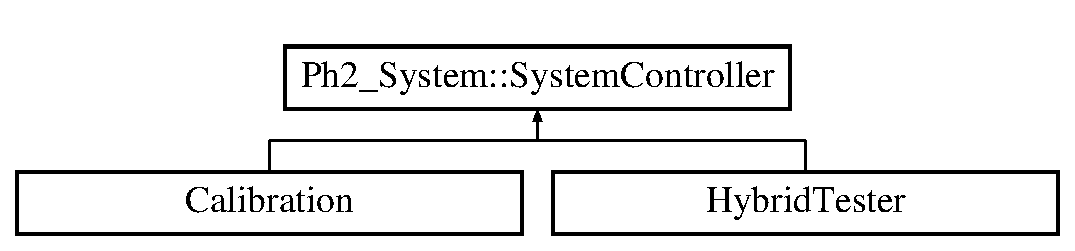
\includegraphics[height=2.000000cm]{class_ph2___system_1_1_system_controller}
\end{center}
\end{figure}
\subsection*{Public Member Functions}
\begin{DoxyCompactItemize}
\item 
\hyperlink{class_ph2___system_1_1_system_controller_a7755f0304eb845c975862df469f25e70}{System\-Controller} ()
\begin{DoxyCompactList}\small\item\em Constructor of the \hyperlink{class_ph2___system_1_1_system_controller}{System\-Controller} class. \end{DoxyCompactList}\item 
\hyperlink{class_ph2___system_1_1_system_controller_abd794b0a85d9d83ec553d707875efcf1}{$\sim$\-System\-Controller} ()
\begin{DoxyCompactList}\small\item\em Destructor of the \hyperlink{class_ph2___system_1_1_system_controller}{System\-Controller} class. \end{DoxyCompactList}\item 
void \hyperlink{class_ph2___system_1_1_system_controller_ab6db20a430b09bd7888d7af0fb3b9511}{Initialize\-Hw} (const char $\ast$p\-Filename)
\begin{DoxyCompactList}\small\item\em Initialize the Hardware via an X\-M\-L file. \end{DoxyCompactList}\item 
void \hyperlink{class_ph2___system_1_1_system_controller_a9f1a7ff3ebeafde5f6e608842a139edb}{Initialize\-Settings} (const char $\ast$p\-Filename)
\begin{DoxyCompactList}\small\item\em Initialize the settings. \end{DoxyCompactList}\item 
void \hyperlink{class_ph2___system_1_1_system_controller_af0bb978523eb3a6436650d9e4f112432}{Configure\-Hw} ()
\begin{DoxyCompactList}\small\item\em Configure the Hardware with X\-M\-L file indicated values. \end{DoxyCompactList}\item 
void \hyperlink{class_ph2___system_1_1_system_controller_a566a9fd32ddb038dc935de263a0032f8}{Run} (\hyperlink{class_ph2___hw_description_1_1_be_board}{Be\-Board} $\ast$p\-Be\-Board, uint32\-\_\-t p\-Nth\-Acq)
\begin{DoxyCompactList}\small\item\em Run a D\-A\-Q. \end{DoxyCompactList}\end{DoxyCompactItemize}
\subsection*{Data Fields}
\begin{DoxyCompactItemize}
\item 
\hyperlink{class_ph2___hw_interface_1_1_be_board_interface}{Be\-Board\-Interface} $\ast$ \hyperlink{class_ph2___system_1_1_system_controller_a8e8bc5e14aaf6659673c16c7dea5e57d}{f\-Be\-Board\-Interface}
\item 
\hyperlink{class_ph2___hw_interface_1_1_cbc_interface}{Cbc\-Interface} $\ast$ \hyperlink{class_ph2___system_1_1_system_controller_ae38e8bcea2b76c5981d2b0e49559ad16}{f\-Cbc\-Interface}
\item 
\hyperlink{namespace_ph2___system_a1c21eed494ab8a888694adf3de379dcf}{Shelve\-Vec} \hyperlink{class_ph2___system_1_1_system_controller_ad98d8c88b5d4138921591ea2c971f714}{f\-Shelve\-Vec}
\item 
\hyperlink{namespace_ph2___hw_interface_ac35d341eb47fa7cbe4d28ccbc6ab4875}{Be\-Board\-F\-W\-Map} \hyperlink{class_ph2___system_1_1_system_controller_a84042bff8bf08490a04e82bdeea9c7d6}{f\-Be\-Board\-F\-W\-Map}
\item 
\hyperlink{namespace_ph2___system_a0ea674c0ee02ac6834ac9a1335111980}{Settings\-Map} \hyperlink{class_ph2___system_1_1_system_controller_a18fd8d1b9c57b411097430646e1dda9a}{f\-Settings\-Map}
\end{DoxyCompactItemize}


\subsection{Detailed Description}
Create, initialise, configure a predefined H\-W structure. 

\subsection{Constructor \& Destructor Documentation}
\hypertarget{class_ph2___system_1_1_system_controller_a7755f0304eb845c975862df469f25e70}{\index{Ph2\-\_\-\-System\-::\-System\-Controller@{Ph2\-\_\-\-System\-::\-System\-Controller}!System\-Controller@{System\-Controller}}
\index{System\-Controller@{System\-Controller}!Ph2_System::SystemController@{Ph2\-\_\-\-System\-::\-System\-Controller}}
\subsubsection[{System\-Controller}]{\setlength{\rightskip}{0pt plus 5cm}Ph2\-\_\-\-System\-::\-System\-Controller\-::\-System\-Controller (
\begin{DoxyParamCaption}
{}
\end{DoxyParamCaption}
)}}\label{class_ph2___system_1_1_system_controller_a7755f0304eb845c975862df469f25e70}


Constructor of the \hyperlink{class_ph2___system_1_1_system_controller}{System\-Controller} class. 

\hypertarget{class_ph2___system_1_1_system_controller_abd794b0a85d9d83ec553d707875efcf1}{\index{Ph2\-\_\-\-System\-::\-System\-Controller@{Ph2\-\_\-\-System\-::\-System\-Controller}!$\sim$\-System\-Controller@{$\sim$\-System\-Controller}}
\index{$\sim$\-System\-Controller@{$\sim$\-System\-Controller}!Ph2_System::SystemController@{Ph2\-\_\-\-System\-::\-System\-Controller}}
\subsubsection[{$\sim$\-System\-Controller}]{\setlength{\rightskip}{0pt plus 5cm}Ph2\-\_\-\-System\-::\-System\-Controller\-::$\sim$\-System\-Controller (
\begin{DoxyParamCaption}
{}
\end{DoxyParamCaption}
)}}\label{class_ph2___system_1_1_system_controller_abd794b0a85d9d83ec553d707875efcf1}


Destructor of the \hyperlink{class_ph2___system_1_1_system_controller}{System\-Controller} class. 



\subsection{Member Function Documentation}
\hypertarget{class_ph2___system_1_1_system_controller_af0bb978523eb3a6436650d9e4f112432}{\index{Ph2\-\_\-\-System\-::\-System\-Controller@{Ph2\-\_\-\-System\-::\-System\-Controller}!Configure\-Hw@{Configure\-Hw}}
\index{Configure\-Hw@{Configure\-Hw}!Ph2_System::SystemController@{Ph2\-\_\-\-System\-::\-System\-Controller}}
\subsubsection[{Configure\-Hw}]{\setlength{\rightskip}{0pt plus 5cm}void Ph2\-\_\-\-System\-::\-System\-Controller\-::\-Configure\-Hw (
\begin{DoxyParamCaption}
{}
\end{DoxyParamCaption}
)}}\label{class_ph2___system_1_1_system_controller_af0bb978523eb3a6436650d9e4f112432}


Configure the Hardware with X\-M\-L file indicated values. 

\hypertarget{class_ph2___system_1_1_system_controller_ab6db20a430b09bd7888d7af0fb3b9511}{\index{Ph2\-\_\-\-System\-::\-System\-Controller@{Ph2\-\_\-\-System\-::\-System\-Controller}!Initialize\-Hw@{Initialize\-Hw}}
\index{Initialize\-Hw@{Initialize\-Hw}!Ph2_System::SystemController@{Ph2\-\_\-\-System\-::\-System\-Controller}}
\subsubsection[{Initialize\-Hw}]{\setlength{\rightskip}{0pt plus 5cm}void Ph2\-\_\-\-System\-::\-System\-Controller\-::\-Initialize\-Hw (
\begin{DoxyParamCaption}
\item[{const char $\ast$}]{p\-Filename}
\end{DoxyParamCaption}
)}}\label{class_ph2___system_1_1_system_controller_ab6db20a430b09bd7888d7af0fb3b9511}


Initialize the Hardware via an X\-M\-L file. 


\begin{DoxyParams}{Parameters}
{\em p\-Filename} & \-: X\-M\-L H\-W Description file \\
\hline
\end{DoxyParams}
\hypertarget{class_ph2___system_1_1_system_controller_a9f1a7ff3ebeafde5f6e608842a139edb}{\index{Ph2\-\_\-\-System\-::\-System\-Controller@{Ph2\-\_\-\-System\-::\-System\-Controller}!Initialize\-Settings@{Initialize\-Settings}}
\index{Initialize\-Settings@{Initialize\-Settings}!Ph2_System::SystemController@{Ph2\-\_\-\-System\-::\-System\-Controller}}
\subsubsection[{Initialize\-Settings}]{\setlength{\rightskip}{0pt plus 5cm}void Ph2\-\_\-\-System\-::\-System\-Controller\-::\-Initialize\-Settings (
\begin{DoxyParamCaption}
\item[{const char $\ast$}]{p\-Filename}
\end{DoxyParamCaption}
)}}\label{class_ph2___system_1_1_system_controller_a9f1a7ff3ebeafde5f6e608842a139edb}


Initialize the settings. 


\begin{DoxyParams}{Parameters}
{\em p\-Filename} & \-: X\-M\-L H\-W Description file \\
\hline
\end{DoxyParams}
\hypertarget{class_ph2___system_1_1_system_controller_a566a9fd32ddb038dc935de263a0032f8}{\index{Ph2\-\_\-\-System\-::\-System\-Controller@{Ph2\-\_\-\-System\-::\-System\-Controller}!Run@{Run}}
\index{Run@{Run}!Ph2_System::SystemController@{Ph2\-\_\-\-System\-::\-System\-Controller}}
\subsubsection[{Run}]{\setlength{\rightskip}{0pt plus 5cm}void Ph2\-\_\-\-System\-::\-System\-Controller\-::\-Run (
\begin{DoxyParamCaption}
\item[{{\bf Be\-Board} $\ast$}]{p\-Be\-Board, }
\item[{uint32\-\_\-t}]{p\-Nth\-Acq}
\end{DoxyParamCaption}
)}}\label{class_ph2___system_1_1_system_controller_a566a9fd32ddb038dc935de263a0032f8}


Run a D\-A\-Q. 


\begin{DoxyParams}{Parameters}
{\em p\-Be\-Board} & \\
\hline
{\em p\-Nth\-Acq} & \\
\hline
\end{DoxyParams}


\subsection{Field Documentation}
\hypertarget{class_ph2___system_1_1_system_controller_a84042bff8bf08490a04e82bdeea9c7d6}{\index{Ph2\-\_\-\-System\-::\-System\-Controller@{Ph2\-\_\-\-System\-::\-System\-Controller}!f\-Be\-Board\-F\-W\-Map@{f\-Be\-Board\-F\-W\-Map}}
\index{f\-Be\-Board\-F\-W\-Map@{f\-Be\-Board\-F\-W\-Map}!Ph2_System::SystemController@{Ph2\-\_\-\-System\-::\-System\-Controller}}
\subsubsection[{f\-Be\-Board\-F\-W\-Map}]{\setlength{\rightskip}{0pt plus 5cm}{\bf Be\-Board\-F\-W\-Map} Ph2\-\_\-\-System\-::\-System\-Controller\-::f\-Be\-Board\-F\-W\-Map}}\label{class_ph2___system_1_1_system_controller_a84042bff8bf08490a04e82bdeea9c7d6}
Map of connections to the Be\-Board \hypertarget{class_ph2___system_1_1_system_controller_a8e8bc5e14aaf6659673c16c7dea5e57d}{\index{Ph2\-\_\-\-System\-::\-System\-Controller@{Ph2\-\_\-\-System\-::\-System\-Controller}!f\-Be\-Board\-Interface@{f\-Be\-Board\-Interface}}
\index{f\-Be\-Board\-Interface@{f\-Be\-Board\-Interface}!Ph2_System::SystemController@{Ph2\-\_\-\-System\-::\-System\-Controller}}
\subsubsection[{f\-Be\-Board\-Interface}]{\setlength{\rightskip}{0pt plus 5cm}{\bf Be\-Board\-Interface}$\ast$ Ph2\-\_\-\-System\-::\-System\-Controller\-::f\-Be\-Board\-Interface}}\label{class_ph2___system_1_1_system_controller_a8e8bc5e14aaf6659673c16c7dea5e57d}
Interface to the Be\-Board \hypertarget{class_ph2___system_1_1_system_controller_ae38e8bcea2b76c5981d2b0e49559ad16}{\index{Ph2\-\_\-\-System\-::\-System\-Controller@{Ph2\-\_\-\-System\-::\-System\-Controller}!f\-Cbc\-Interface@{f\-Cbc\-Interface}}
\index{f\-Cbc\-Interface@{f\-Cbc\-Interface}!Ph2_System::SystemController@{Ph2\-\_\-\-System\-::\-System\-Controller}}
\subsubsection[{f\-Cbc\-Interface}]{\setlength{\rightskip}{0pt plus 5cm}{\bf Cbc\-Interface}$\ast$ Ph2\-\_\-\-System\-::\-System\-Controller\-::f\-Cbc\-Interface}}\label{class_ph2___system_1_1_system_controller_ae38e8bcea2b76c5981d2b0e49559ad16}
Interface to the Cbc \hypertarget{class_ph2___system_1_1_system_controller_a18fd8d1b9c57b411097430646e1dda9a}{\index{Ph2\-\_\-\-System\-::\-System\-Controller@{Ph2\-\_\-\-System\-::\-System\-Controller}!f\-Settings\-Map@{f\-Settings\-Map}}
\index{f\-Settings\-Map@{f\-Settings\-Map}!Ph2_System::SystemController@{Ph2\-\_\-\-System\-::\-System\-Controller}}
\subsubsection[{f\-Settings\-Map}]{\setlength{\rightskip}{0pt plus 5cm}{\bf Settings\-Map} Ph2\-\_\-\-System\-::\-System\-Controller\-::f\-Settings\-Map}}\label{class_ph2___system_1_1_system_controller_a18fd8d1b9c57b411097430646e1dda9a}
Maps the settings \hypertarget{class_ph2___system_1_1_system_controller_ad98d8c88b5d4138921591ea2c971f714}{\index{Ph2\-\_\-\-System\-::\-System\-Controller@{Ph2\-\_\-\-System\-::\-System\-Controller}!f\-Shelve\-Vec@{f\-Shelve\-Vec}}
\index{f\-Shelve\-Vec@{f\-Shelve\-Vec}!Ph2_System::SystemController@{Ph2\-\_\-\-System\-::\-System\-Controller}}
\subsubsection[{f\-Shelve\-Vec}]{\setlength{\rightskip}{0pt plus 5cm}{\bf Shelve\-Vec} Ph2\-\_\-\-System\-::\-System\-Controller\-::f\-Shelve\-Vec}}\label{class_ph2___system_1_1_system_controller_ad98d8c88b5d4138921591ea2c971f714}
Vector of Shelve pointers 

The documentation for this class was generated from the following files\-:\begin{DoxyCompactItemize}
\item 
System/\hyperlink{_system_controller_8h}{System\-Controller.\-h}\item 
System/\hyperlink{_system_controller_8cc}{System\-Controller.\-cc}\end{DoxyCompactItemize}

\hypertarget{struct_test_group}{\section{Test\-Group Struct Reference}
\label{struct_test_group}\index{Test\-Group@{Test\-Group}}
}


{\ttfamily \#include $<$Channel.\-h$>$}

\subsection*{Public Member Functions}
\begin{DoxyCompactItemize}
\item 
\hyperlink{struct_test_group_abc9cdcaaaeaf7be5d30db099ca8953cb}{Test\-Group} (uint8\-\_\-t p\-Be\-Id, uint8\-\_\-t p\-Fe\-Id, uint8\-\_\-t p\-Cbc\-Id, uint8\-\_\-t p\-Group\-Id)
\item 
void \hyperlink{struct_test_group_ab2b392dd24e0961bd115c0240d7a25ff}{Fill\-Vplus\-Vcth\-Graph} (uint8\-\_\-t p\-Vplus, double p\-Pedestal, double p\-Noise)
\end{DoxyCompactItemize}
\subsection*{Data Fields}
\begin{DoxyCompactItemize}
\item 
uint8\-\_\-t \hyperlink{struct_test_group_a220aae8ee3ae8c357f1787e3625431b4}{f\-Be\-Id}
\item 
uint8\-\_\-t \hyperlink{struct_test_group_a0eaafe2a6411b3865c90240b36b24840}{f\-Fe\-Id}
\item 
uint8\-\_\-t \hyperlink{struct_test_group_ac29315115540d3e0fc74b2dba3771162}{f\-Cbc\-Id}
\item 
uint8\-\_\-t \hyperlink{struct_test_group_a425092488cd04f3f22fdf8dfe0e877ed}{f\-Group\-Id}
\item 
T\-Graph\-Errors $\ast$ \hyperlink{struct_test_group_a1481302f545d48c3185534280d55b545}{f\-Vplus\-Vcth\-Graph}
\end{DoxyCompactItemize}


\subsection{Constructor \& Destructor Documentation}
\hypertarget{struct_test_group_abc9cdcaaaeaf7be5d30db099ca8953cb}{\index{Test\-Group@{Test\-Group}!Test\-Group@{Test\-Group}}
\index{Test\-Group@{Test\-Group}!TestGroup@{Test\-Group}}
\subsubsection[{Test\-Group}]{\setlength{\rightskip}{0pt plus 5cm}Test\-Group\-::\-Test\-Group (
\begin{DoxyParamCaption}
\item[{uint8\-\_\-t}]{p\-Be\-Id, }
\item[{uint8\-\_\-t}]{p\-Fe\-Id, }
\item[{uint8\-\_\-t}]{p\-Cbc\-Id, }
\item[{uint8\-\_\-t}]{p\-Group\-Id}
\end{DoxyParamCaption}
)}}\label{struct_test_group_abc9cdcaaaeaf7be5d30db099ca8953cb}


\subsection{Member Function Documentation}
\hypertarget{struct_test_group_ab2b392dd24e0961bd115c0240d7a25ff}{\index{Test\-Group@{Test\-Group}!Fill\-Vplus\-Vcth\-Graph@{Fill\-Vplus\-Vcth\-Graph}}
\index{Fill\-Vplus\-Vcth\-Graph@{Fill\-Vplus\-Vcth\-Graph}!TestGroup@{Test\-Group}}
\subsubsection[{Fill\-Vplus\-Vcth\-Graph}]{\setlength{\rightskip}{0pt plus 5cm}void Test\-Group\-::\-Fill\-Vplus\-Vcth\-Graph (
\begin{DoxyParamCaption}
\item[{uint8\-\_\-t}]{p\-Vplus, }
\item[{double}]{p\-Pedestal, }
\item[{double}]{p\-Noise}
\end{DoxyParamCaption}
)}}\label{struct_test_group_ab2b392dd24e0961bd115c0240d7a25ff}


\subsection{Field Documentation}
\hypertarget{struct_test_group_a220aae8ee3ae8c357f1787e3625431b4}{\index{Test\-Group@{Test\-Group}!f\-Be\-Id@{f\-Be\-Id}}
\index{f\-Be\-Id@{f\-Be\-Id}!TestGroup@{Test\-Group}}
\subsubsection[{f\-Be\-Id}]{\setlength{\rightskip}{0pt plus 5cm}uint8\-\_\-t Test\-Group\-::f\-Be\-Id}}\label{struct_test_group_a220aae8ee3ae8c357f1787e3625431b4}
\hypertarget{struct_test_group_ac29315115540d3e0fc74b2dba3771162}{\index{Test\-Group@{Test\-Group}!f\-Cbc\-Id@{f\-Cbc\-Id}}
\index{f\-Cbc\-Id@{f\-Cbc\-Id}!TestGroup@{Test\-Group}}
\subsubsection[{f\-Cbc\-Id}]{\setlength{\rightskip}{0pt plus 5cm}uint8\-\_\-t Test\-Group\-::f\-Cbc\-Id}}\label{struct_test_group_ac29315115540d3e0fc74b2dba3771162}
\hypertarget{struct_test_group_a0eaafe2a6411b3865c90240b36b24840}{\index{Test\-Group@{Test\-Group}!f\-Fe\-Id@{f\-Fe\-Id}}
\index{f\-Fe\-Id@{f\-Fe\-Id}!TestGroup@{Test\-Group}}
\subsubsection[{f\-Fe\-Id}]{\setlength{\rightskip}{0pt plus 5cm}uint8\-\_\-t Test\-Group\-::f\-Fe\-Id}}\label{struct_test_group_a0eaafe2a6411b3865c90240b36b24840}
\hypertarget{struct_test_group_a425092488cd04f3f22fdf8dfe0e877ed}{\index{Test\-Group@{Test\-Group}!f\-Group\-Id@{f\-Group\-Id}}
\index{f\-Group\-Id@{f\-Group\-Id}!TestGroup@{Test\-Group}}
\subsubsection[{f\-Group\-Id}]{\setlength{\rightskip}{0pt plus 5cm}uint8\-\_\-t Test\-Group\-::f\-Group\-Id}}\label{struct_test_group_a425092488cd04f3f22fdf8dfe0e877ed}
\hypertarget{struct_test_group_a1481302f545d48c3185534280d55b545}{\index{Test\-Group@{Test\-Group}!f\-Vplus\-Vcth\-Graph@{f\-Vplus\-Vcth\-Graph}}
\index{f\-Vplus\-Vcth\-Graph@{f\-Vplus\-Vcth\-Graph}!TestGroup@{Test\-Group}}
\subsubsection[{f\-Vplus\-Vcth\-Graph}]{\setlength{\rightskip}{0pt plus 5cm}T\-Graph\-Errors$\ast$ Test\-Group\-::f\-Vplus\-Vcth\-Graph}}\label{struct_test_group_a1481302f545d48c3185534280d55b545}


The documentation for this struct was generated from the following files\-:\begin{DoxyCompactItemize}
\item 
tools/\hyperlink{_channel_8h}{Channel.\-h}\item 
tools/\hyperlink{_channel_8cc}{Channel.\-cc}\end{DoxyCompactItemize}

\hypertarget{struct_test_group_comparer}{
\section{Test\-Group\-Comparer Struct Reference}
\label{struct_test_group_comparer}\index{TestGroupComparer@{TestGroupComparer}}
}
{\tt \#include $<$Channel.h$>$}

\subsection*{Public Member Functions}
\begin{CompactItemize}
\item 
bool \hyperlink{struct_test_group_comparer_f1d4d79824e65c08f7e063f6d09eb755}{operator()} (const \hyperlink{struct_test_group}{Test\-Group} \&g1, const \hyperlink{struct_test_group}{Test\-Group} \&g2) const 
\end{CompactItemize}


\subsection{Member Function Documentation}
\hypertarget{struct_test_group_comparer_f1d4d79824e65c08f7e063f6d09eb755}{
\index{TestGroupComparer@{Test\-Group\-Comparer}!operator()@{operator()}}
\index{operator()@{operator()}!TestGroupComparer@{Test\-Group\-Comparer}}
\subsubsection[operator()]{\setlength{\rightskip}{0pt plus 5cm}bool Test\-Group\-Comparer::operator() (const \hyperlink{struct_test_group}{Test\-Group} \& {\em g1}, const \hyperlink{struct_test_group}{Test\-Group} \& {\em g2}) const\hspace{0.3cm}{\tt  \mbox{[}inline\mbox{]}}}}
\label{struct_test_group_comparer_f1d4d79824e65c08f7e063f6d09eb755}




The documentation for this struct was generated from the following file:\begin{CompactItemize}
\item 
tools/\hyperlink{_channel_8h}{Channel.h}\end{CompactItemize}

\hypertarget{structutf16__counter}{
\section{utf16\_\-counter Struct Reference}
\label{structutf16__counter}\index{utf16_counter@{utf16\_\-counter}}
}
\subsection*{Public Types}
\begin{CompactItemize}
\item 
typedef size\_\-t \hyperlink{structutf16__counter_0d63f9ca809d182b2f184ef93bd11107}{value\_\-type}
\end{CompactItemize}
\subsection*{Static Public Member Functions}
\begin{CompactItemize}
\item 
static \hyperlink{structutf16__counter_0d63f9ca809d182b2f184ef93bd11107}{value\_\-type} \hyperlink{structutf16__counter_4571f3d0fbf0ce763904ec3321dcb41e}{low} (\hyperlink{structutf16__counter_0d63f9ca809d182b2f184ef93bd11107}{value\_\-type} result, uint32\_\-t)
\item 
static \hyperlink{structutf16__counter_0d63f9ca809d182b2f184ef93bd11107}{value\_\-type} \hyperlink{structutf16__counter_c1a8793996e57dc28fd22f3165628e4d}{high} (\hyperlink{structutf16__counter_0d63f9ca809d182b2f184ef93bd11107}{value\_\-type} result, uint32\_\-t)
\end{CompactItemize}


\subsection{Member Typedef Documentation}
\hypertarget{structutf16__counter_0d63f9ca809d182b2f184ef93bd11107}{
\index{utf16_counter@{utf16\_\-counter}!value_type@{value\_\-type}}
\index{value_type@{value\_\-type}!utf16_counter@{utf16\_\-counter}}
\subsubsection[value\_\-type]{\setlength{\rightskip}{0pt plus 5cm}typedef size\_\-t \hyperlink{structutf16__counter_0d63f9ca809d182b2f184ef93bd11107}{utf16\_\-counter::value\_\-type}}}
\label{structutf16__counter_0d63f9ca809d182b2f184ef93bd11107}




\subsection{Member Function Documentation}
\hypertarget{structutf16__counter_c1a8793996e57dc28fd22f3165628e4d}{
\index{utf16_counter@{utf16\_\-counter}!high@{high}}
\index{high@{high}!utf16_counter@{utf16\_\-counter}}
\subsubsection[high]{\setlength{\rightskip}{0pt plus 5cm}static \hyperlink{structutf16__counter_0d63f9ca809d182b2f184ef93bd11107}{value\_\-type} utf16\_\-counter::high (\hyperlink{structutf16__counter_0d63f9ca809d182b2f184ef93bd11107}{value\_\-type} {\em result}, uint32\_\-t)\hspace{0.3cm}{\tt  \mbox{[}inline, static\mbox{]}}}}
\label{structutf16__counter_c1a8793996e57dc28fd22f3165628e4d}


\hypertarget{structutf16__counter_4571f3d0fbf0ce763904ec3321dcb41e}{
\index{utf16_counter@{utf16\_\-counter}!low@{low}}
\index{low@{low}!utf16_counter@{utf16\_\-counter}}
\subsubsection[low]{\setlength{\rightskip}{0pt plus 5cm}static \hyperlink{structutf16__counter_0d63f9ca809d182b2f184ef93bd11107}{value\_\-type} utf16\_\-counter::low (\hyperlink{structutf16__counter_0d63f9ca809d182b2f184ef93bd11107}{value\_\-type} {\em result}, uint32\_\-t)\hspace{0.3cm}{\tt  \mbox{[}inline, static\mbox{]}}}}
\label{structutf16__counter_4571f3d0fbf0ce763904ec3321dcb41e}




The documentation for this struct was generated from the following file:\begin{CompactItemize}
\item 
Utils/\hyperlink{pugixml_8cpp}{pugixml.cpp}\end{CompactItemize}

\hypertarget{structutf16__writer}{
\section{utf16\_\-writer Struct Reference}
\label{structutf16__writer}\index{utf16_writer@{utf16\_\-writer}}
}
\subsection*{Public Types}
\begin{CompactItemize}
\item 
typedef uint16\_\-t $\ast$ \hyperlink{structutf16__writer_527b705eaf5099167b8bc42423ce918c}{value\_\-type}
\end{CompactItemize}
\subsection*{Static Public Member Functions}
\begin{CompactItemize}
\item 
static \hyperlink{structutf16__writer_527b705eaf5099167b8bc42423ce918c}{value\_\-type} \hyperlink{structutf16__writer_b11fef721a8b38de5e315d2e75d12956}{low} (\hyperlink{structutf16__writer_527b705eaf5099167b8bc42423ce918c}{value\_\-type} result, uint32\_\-t ch)
\item 
static \hyperlink{structutf16__writer_527b705eaf5099167b8bc42423ce918c}{value\_\-type} \hyperlink{structutf16__writer_01b6ce1a567dea11daead3ca83f42d5c}{high} (\hyperlink{structutf16__writer_527b705eaf5099167b8bc42423ce918c}{value\_\-type} result, uint32\_\-t ch)
\item 
static \hyperlink{structutf16__writer_527b705eaf5099167b8bc42423ce918c}{value\_\-type} \hyperlink{structutf16__writer_c14e06db126fbbef4be7efdb80fbdf4a}{any} (\hyperlink{structutf16__writer_527b705eaf5099167b8bc42423ce918c}{value\_\-type} result, uint32\_\-t ch)
\end{CompactItemize}


\subsection{Member Typedef Documentation}
\hypertarget{structutf16__writer_527b705eaf5099167b8bc42423ce918c}{
\index{utf16_writer@{utf16\_\-writer}!value_type@{value\_\-type}}
\index{value_type@{value\_\-type}!utf16_writer@{utf16\_\-writer}}
\subsubsection[value\_\-type]{\setlength{\rightskip}{0pt plus 5cm}typedef uint16\_\-t$\ast$ \hyperlink{structutf16__writer_527b705eaf5099167b8bc42423ce918c}{utf16\_\-writer::value\_\-type}}}
\label{structutf16__writer_527b705eaf5099167b8bc42423ce918c}




\subsection{Member Function Documentation}
\hypertarget{structutf16__writer_c14e06db126fbbef4be7efdb80fbdf4a}{
\index{utf16_writer@{utf16\_\-writer}!any@{any}}
\index{any@{any}!utf16_writer@{utf16\_\-writer}}
\subsubsection[any]{\setlength{\rightskip}{0pt plus 5cm}static \hyperlink{structutf16__writer_527b705eaf5099167b8bc42423ce918c}{value\_\-type} utf16\_\-writer::any (\hyperlink{structutf16__writer_527b705eaf5099167b8bc42423ce918c}{value\_\-type} {\em result}, uint32\_\-t {\em ch})\hspace{0.3cm}{\tt  \mbox{[}inline, static\mbox{]}}}}
\label{structutf16__writer_c14e06db126fbbef4be7efdb80fbdf4a}


\hypertarget{structutf16__writer_01b6ce1a567dea11daead3ca83f42d5c}{
\index{utf16_writer@{utf16\_\-writer}!high@{high}}
\index{high@{high}!utf16_writer@{utf16\_\-writer}}
\subsubsection[high]{\setlength{\rightskip}{0pt plus 5cm}static \hyperlink{structutf16__writer_527b705eaf5099167b8bc42423ce918c}{value\_\-type} utf16\_\-writer::high (\hyperlink{structutf16__writer_527b705eaf5099167b8bc42423ce918c}{value\_\-type} {\em result}, uint32\_\-t {\em ch})\hspace{0.3cm}{\tt  \mbox{[}inline, static\mbox{]}}}}
\label{structutf16__writer_01b6ce1a567dea11daead3ca83f42d5c}


\hypertarget{structutf16__writer_b11fef721a8b38de5e315d2e75d12956}{
\index{utf16_writer@{utf16\_\-writer}!low@{low}}
\index{low@{low}!utf16_writer@{utf16\_\-writer}}
\subsubsection[low]{\setlength{\rightskip}{0pt plus 5cm}static \hyperlink{structutf16__writer_527b705eaf5099167b8bc42423ce918c}{value\_\-type} utf16\_\-writer::low (\hyperlink{structutf16__writer_527b705eaf5099167b8bc42423ce918c}{value\_\-type} {\em result}, uint32\_\-t {\em ch})\hspace{0.3cm}{\tt  \mbox{[}inline, static\mbox{]}}}}
\label{structutf16__writer_b11fef721a8b38de5e315d2e75d12956}




The documentation for this struct was generated from the following file:\begin{CompactItemize}
\item 
Utils/\hyperlink{pugixml_8cpp}{pugixml.cpp}\end{CompactItemize}

\hypertarget{structutf32__counter}{\section{utf32\-\_\-counter Struct Reference}
\label{structutf32__counter}\index{utf32\-\_\-counter@{utf32\-\_\-counter}}
}
\subsection*{Public Types}
\begin{DoxyCompactItemize}
\item 
typedef size\-\_\-t \hyperlink{structutf32__counter_a6fb6728fe1a009958000f0e934fa6500}{value\-\_\-type}
\end{DoxyCompactItemize}
\subsection*{Static Public Member Functions}
\begin{DoxyCompactItemize}
\item 
static \hyperlink{structutf32__counter_a6fb6728fe1a009958000f0e934fa6500}{value\-\_\-type} \hyperlink{structutf32__counter_a3a75f4840e0391ed972ddba621d49480}{low} (\hyperlink{structutf32__counter_a6fb6728fe1a009958000f0e934fa6500}{value\-\_\-type} result, uint32\-\_\-t)
\item 
static \hyperlink{structutf32__counter_a6fb6728fe1a009958000f0e934fa6500}{value\-\_\-type} \hyperlink{structutf32__counter_aa72f5248b1dc5937330ab049bf449251}{high} (\hyperlink{structutf32__counter_a6fb6728fe1a009958000f0e934fa6500}{value\-\_\-type} result, uint32\-\_\-t)
\end{DoxyCompactItemize}


\subsection{Member Typedef Documentation}
\hypertarget{structutf32__counter_a6fb6728fe1a009958000f0e934fa6500}{\index{utf32\-\_\-counter@{utf32\-\_\-counter}!value\-\_\-type@{value\-\_\-type}}
\index{value\-\_\-type@{value\-\_\-type}!utf32_counter@{utf32\-\_\-counter}}
\subsubsection[{value\-\_\-type}]{\setlength{\rightskip}{0pt plus 5cm}typedef size\-\_\-t {\bf utf32\-\_\-counter\-::value\-\_\-type}}}\label{structutf32__counter_a6fb6728fe1a009958000f0e934fa6500}


\subsection{Member Function Documentation}
\hypertarget{structutf32__counter_aa72f5248b1dc5937330ab049bf449251}{\index{utf32\-\_\-counter@{utf32\-\_\-counter}!high@{high}}
\index{high@{high}!utf32_counter@{utf32\-\_\-counter}}
\subsubsection[{high}]{\setlength{\rightskip}{0pt plus 5cm}static {\bf value\-\_\-type} utf32\-\_\-counter\-::high (
\begin{DoxyParamCaption}
\item[{{\bf value\-\_\-type}}]{result, }
\item[{uint32\-\_\-t}]{}
\end{DoxyParamCaption}
)\hspace{0.3cm}{\ttfamily [inline]}, {\ttfamily [static]}}}\label{structutf32__counter_aa72f5248b1dc5937330ab049bf449251}
\hypertarget{structutf32__counter_a3a75f4840e0391ed972ddba621d49480}{\index{utf32\-\_\-counter@{utf32\-\_\-counter}!low@{low}}
\index{low@{low}!utf32_counter@{utf32\-\_\-counter}}
\subsubsection[{low}]{\setlength{\rightskip}{0pt plus 5cm}static {\bf value\-\_\-type} utf32\-\_\-counter\-::low (
\begin{DoxyParamCaption}
\item[{{\bf value\-\_\-type}}]{result, }
\item[{uint32\-\_\-t}]{}
\end{DoxyParamCaption}
)\hspace{0.3cm}{\ttfamily [inline]}, {\ttfamily [static]}}}\label{structutf32__counter_a3a75f4840e0391ed972ddba621d49480}


The documentation for this struct was generated from the following file\-:\begin{DoxyCompactItemize}
\item 
System/\hyperlink{pugixml_8cpp}{pugixml.\-cpp}\end{DoxyCompactItemize}

\hypertarget{structutf32__writer}{
\section{utf32\_\-writer Struct Reference}
\label{structutf32__writer}\index{utf32_writer@{utf32\_\-writer}}
}
\subsection*{Public Types}
\begin{CompactItemize}
\item 
typedef uint32\_\-t $\ast$ \hyperlink{structutf32__writer_2284e1fa3406f113f151ded2aaa8d4ae}{value\_\-type}
\end{CompactItemize}
\subsection*{Static Public Member Functions}
\begin{CompactItemize}
\item 
static \hyperlink{structutf32__writer_2284e1fa3406f113f151ded2aaa8d4ae}{value\_\-type} \hyperlink{structutf32__writer_06e1b65906f7355ea54a622248095bc7}{low} (\hyperlink{structutf32__writer_2284e1fa3406f113f151ded2aaa8d4ae}{value\_\-type} result, uint32\_\-t ch)
\item 
static \hyperlink{structutf32__writer_2284e1fa3406f113f151ded2aaa8d4ae}{value\_\-type} \hyperlink{structutf32__writer_3f86d996cde3ed7cab5c31930b67c9f1}{high} (\hyperlink{structutf32__writer_2284e1fa3406f113f151ded2aaa8d4ae}{value\_\-type} result, uint32\_\-t ch)
\item 
static \hyperlink{structutf32__writer_2284e1fa3406f113f151ded2aaa8d4ae}{value\_\-type} \hyperlink{structutf32__writer_a94aaa4a13e755942e7da70ea7700d3e}{any} (\hyperlink{structutf32__writer_2284e1fa3406f113f151ded2aaa8d4ae}{value\_\-type} result, uint32\_\-t ch)
\end{CompactItemize}


\subsection{Member Typedef Documentation}
\hypertarget{structutf32__writer_2284e1fa3406f113f151ded2aaa8d4ae}{
\index{utf32_writer@{utf32\_\-writer}!value_type@{value\_\-type}}
\index{value_type@{value\_\-type}!utf32_writer@{utf32\_\-writer}}
\subsubsection[value\_\-type]{\setlength{\rightskip}{0pt plus 5cm}typedef uint32\_\-t$\ast$ \hyperlink{structutf32__writer_2284e1fa3406f113f151ded2aaa8d4ae}{utf32\_\-writer::value\_\-type}}}
\label{structutf32__writer_2284e1fa3406f113f151ded2aaa8d4ae}




\subsection{Member Function Documentation}
\hypertarget{structutf32__writer_a94aaa4a13e755942e7da70ea7700d3e}{
\index{utf32_writer@{utf32\_\-writer}!any@{any}}
\index{any@{any}!utf32_writer@{utf32\_\-writer}}
\subsubsection[any]{\setlength{\rightskip}{0pt plus 5cm}static \hyperlink{structutf32__writer_2284e1fa3406f113f151ded2aaa8d4ae}{value\_\-type} utf32\_\-writer::any (\hyperlink{structutf32__writer_2284e1fa3406f113f151ded2aaa8d4ae}{value\_\-type} {\em result}, uint32\_\-t {\em ch})\hspace{0.3cm}{\tt  \mbox{[}inline, static\mbox{]}}}}
\label{structutf32__writer_a94aaa4a13e755942e7da70ea7700d3e}


\hypertarget{structutf32__writer_3f86d996cde3ed7cab5c31930b67c9f1}{
\index{utf32_writer@{utf32\_\-writer}!high@{high}}
\index{high@{high}!utf32_writer@{utf32\_\-writer}}
\subsubsection[high]{\setlength{\rightskip}{0pt plus 5cm}static \hyperlink{structutf32__writer_2284e1fa3406f113f151ded2aaa8d4ae}{value\_\-type} utf32\_\-writer::high (\hyperlink{structutf32__writer_2284e1fa3406f113f151ded2aaa8d4ae}{value\_\-type} {\em result}, uint32\_\-t {\em ch})\hspace{0.3cm}{\tt  \mbox{[}inline, static\mbox{]}}}}
\label{structutf32__writer_3f86d996cde3ed7cab5c31930b67c9f1}


\hypertarget{structutf32__writer_06e1b65906f7355ea54a622248095bc7}{
\index{utf32_writer@{utf32\_\-writer}!low@{low}}
\index{low@{low}!utf32_writer@{utf32\_\-writer}}
\subsubsection[low]{\setlength{\rightskip}{0pt plus 5cm}static \hyperlink{structutf32__writer_2284e1fa3406f113f151ded2aaa8d4ae}{value\_\-type} utf32\_\-writer::low (\hyperlink{structutf32__writer_2284e1fa3406f113f151ded2aaa8d4ae}{value\_\-type} {\em result}, uint32\_\-t {\em ch})\hspace{0.3cm}{\tt  \mbox{[}inline, static\mbox{]}}}}
\label{structutf32__writer_06e1b65906f7355ea54a622248095bc7}




The documentation for this struct was generated from the following file:\begin{CompactItemize}
\item 
Utils/\hyperlink{pugixml_8cpp}{pugixml.cpp}\end{CompactItemize}

\hypertarget{structutf8__counter}{\section{utf8\-\_\-counter Struct Reference}
\label{structutf8__counter}\index{utf8\-\_\-counter@{utf8\-\_\-counter}}
}
\subsection*{Public Types}
\begin{DoxyCompactItemize}
\item 
typedef size\-\_\-t \hyperlink{structutf8__counter_adb65152c007965c42184614da9c4af1b}{value\-\_\-type}
\end{DoxyCompactItemize}
\subsection*{Static Public Member Functions}
\begin{DoxyCompactItemize}
\item 
static \hyperlink{structutf8__counter_adb65152c007965c42184614da9c4af1b}{value\-\_\-type} \hyperlink{structutf8__counter_a0950643189089175ae0eac9b4193534d}{low} (\hyperlink{structutf8__counter_adb65152c007965c42184614da9c4af1b}{value\-\_\-type} result, uint32\-\_\-t ch)
\item 
static \hyperlink{structutf8__counter_adb65152c007965c42184614da9c4af1b}{value\-\_\-type} \hyperlink{structutf8__counter_ab16e675980a15e1ede2e4cd18d19f7b1}{high} (\hyperlink{structutf8__counter_adb65152c007965c42184614da9c4af1b}{value\-\_\-type} result, uint32\-\_\-t)
\end{DoxyCompactItemize}


\subsection{Member Typedef Documentation}
\hypertarget{structutf8__counter_adb65152c007965c42184614da9c4af1b}{\index{utf8\-\_\-counter@{utf8\-\_\-counter}!value\-\_\-type@{value\-\_\-type}}
\index{value\-\_\-type@{value\-\_\-type}!utf8_counter@{utf8\-\_\-counter}}
\subsubsection[{value\-\_\-type}]{\setlength{\rightskip}{0pt plus 5cm}typedef size\-\_\-t {\bf utf8\-\_\-counter\-::value\-\_\-type}}}\label{structutf8__counter_adb65152c007965c42184614da9c4af1b}


\subsection{Member Function Documentation}
\hypertarget{structutf8__counter_ab16e675980a15e1ede2e4cd18d19f7b1}{\index{utf8\-\_\-counter@{utf8\-\_\-counter}!high@{high}}
\index{high@{high}!utf8_counter@{utf8\-\_\-counter}}
\subsubsection[{high}]{\setlength{\rightskip}{0pt plus 5cm}static {\bf value\-\_\-type} utf8\-\_\-counter\-::high (
\begin{DoxyParamCaption}
\item[{{\bf value\-\_\-type}}]{result, }
\item[{uint32\-\_\-t}]{}
\end{DoxyParamCaption}
)\hspace{0.3cm}{\ttfamily [inline]}, {\ttfamily [static]}}}\label{structutf8__counter_ab16e675980a15e1ede2e4cd18d19f7b1}
\hypertarget{structutf8__counter_a0950643189089175ae0eac9b4193534d}{\index{utf8\-\_\-counter@{utf8\-\_\-counter}!low@{low}}
\index{low@{low}!utf8_counter@{utf8\-\_\-counter}}
\subsubsection[{low}]{\setlength{\rightskip}{0pt plus 5cm}static {\bf value\-\_\-type} utf8\-\_\-counter\-::low (
\begin{DoxyParamCaption}
\item[{{\bf value\-\_\-type}}]{result, }
\item[{uint32\-\_\-t}]{ch}
\end{DoxyParamCaption}
)\hspace{0.3cm}{\ttfamily [inline]}, {\ttfamily [static]}}}\label{structutf8__counter_a0950643189089175ae0eac9b4193534d}


The documentation for this struct was generated from the following file\-:\begin{DoxyCompactItemize}
\item 
System/\hyperlink{pugixml_8cpp}{pugixml.\-cpp}\end{DoxyCompactItemize}

\hypertarget{structutf8__writer}{\section{utf8\-\_\-writer Struct Reference}
\label{structutf8__writer}\index{utf8\-\_\-writer@{utf8\-\_\-writer}}
}
\subsection*{Public Types}
\begin{DoxyCompactItemize}
\item 
typedef uint8\-\_\-t $\ast$ \hyperlink{structutf8__writer_af25ec3c651f9a4a3f193573a4e95002b}{value\-\_\-type}
\end{DoxyCompactItemize}
\subsection*{Static Public Member Functions}
\begin{DoxyCompactItemize}
\item 
static \hyperlink{structutf8__writer_af25ec3c651f9a4a3f193573a4e95002b}{value\-\_\-type} \hyperlink{structutf8__writer_ac4ec52da6f37225ba4fde259bff2f86c}{low} (\hyperlink{structutf8__writer_af25ec3c651f9a4a3f193573a4e95002b}{value\-\_\-type} result, uint32\-\_\-t ch)
\item 
static \hyperlink{structutf8__writer_af25ec3c651f9a4a3f193573a4e95002b}{value\-\_\-type} \hyperlink{structutf8__writer_ac03dfaf797d599afdf0be7def86ff9b9}{high} (\hyperlink{structutf8__writer_af25ec3c651f9a4a3f193573a4e95002b}{value\-\_\-type} result, uint32\-\_\-t ch)
\item 
static \hyperlink{structutf8__writer_af25ec3c651f9a4a3f193573a4e95002b}{value\-\_\-type} \hyperlink{structutf8__writer_a288e9c5f3720b95ae6b77330ad38dd56}{any} (\hyperlink{structutf8__writer_af25ec3c651f9a4a3f193573a4e95002b}{value\-\_\-type} result, uint32\-\_\-t ch)
\end{DoxyCompactItemize}


\subsection{Member Typedef Documentation}
\hypertarget{structutf8__writer_af25ec3c651f9a4a3f193573a4e95002b}{\index{utf8\-\_\-writer@{utf8\-\_\-writer}!value\-\_\-type@{value\-\_\-type}}
\index{value\-\_\-type@{value\-\_\-type}!utf8_writer@{utf8\-\_\-writer}}
\subsubsection[{value\-\_\-type}]{\setlength{\rightskip}{0pt plus 5cm}typedef uint8\-\_\-t$\ast$ {\bf utf8\-\_\-writer\-::value\-\_\-type}}}\label{structutf8__writer_af25ec3c651f9a4a3f193573a4e95002b}


\subsection{Member Function Documentation}
\hypertarget{structutf8__writer_a288e9c5f3720b95ae6b77330ad38dd56}{\index{utf8\-\_\-writer@{utf8\-\_\-writer}!any@{any}}
\index{any@{any}!utf8_writer@{utf8\-\_\-writer}}
\subsubsection[{any}]{\setlength{\rightskip}{0pt plus 5cm}static {\bf value\-\_\-type} utf8\-\_\-writer\-::any (
\begin{DoxyParamCaption}
\item[{{\bf value\-\_\-type}}]{result, }
\item[{uint32\-\_\-t}]{ch}
\end{DoxyParamCaption}
)\hspace{0.3cm}{\ttfamily [inline]}, {\ttfamily [static]}}}\label{structutf8__writer_a288e9c5f3720b95ae6b77330ad38dd56}
\hypertarget{structutf8__writer_ac03dfaf797d599afdf0be7def86ff9b9}{\index{utf8\-\_\-writer@{utf8\-\_\-writer}!high@{high}}
\index{high@{high}!utf8_writer@{utf8\-\_\-writer}}
\subsubsection[{high}]{\setlength{\rightskip}{0pt plus 5cm}static {\bf value\-\_\-type} utf8\-\_\-writer\-::high (
\begin{DoxyParamCaption}
\item[{{\bf value\-\_\-type}}]{result, }
\item[{uint32\-\_\-t}]{ch}
\end{DoxyParamCaption}
)\hspace{0.3cm}{\ttfamily [inline]}, {\ttfamily [static]}}}\label{structutf8__writer_ac03dfaf797d599afdf0be7def86ff9b9}
\hypertarget{structutf8__writer_ac4ec52da6f37225ba4fde259bff2f86c}{\index{utf8\-\_\-writer@{utf8\-\_\-writer}!low@{low}}
\index{low@{low}!utf8_writer@{utf8\-\_\-writer}}
\subsubsection[{low}]{\setlength{\rightskip}{0pt plus 5cm}static {\bf value\-\_\-type} utf8\-\_\-writer\-::low (
\begin{DoxyParamCaption}
\item[{{\bf value\-\_\-type}}]{result, }
\item[{uint32\-\_\-t}]{ch}
\end{DoxyParamCaption}
)\hspace{0.3cm}{\ttfamily [inline]}, {\ttfamily [static]}}}\label{structutf8__writer_ac4ec52da6f37225ba4fde259bff2f86c}


The documentation for this struct was generated from the following file\-:\begin{DoxyCompactItemize}
\item 
System/\hyperlink{pugixml_8cpp}{pugixml.\-cpp}\end{DoxyCompactItemize}

\hypertarget{structutf__decoder}{\section{utf\-\_\-decoder$<$ Traits, opt\-\_\-swap $>$ Struct Template Reference}
\label{structutf__decoder}\index{utf\-\_\-decoder$<$ Traits, opt\-\_\-swap $>$@{utf\-\_\-decoder$<$ Traits, opt\-\_\-swap $>$}}
}
\subsection*{Static Public Member Functions}
\begin{DoxyCompactItemize}
\item 
static Traits\-::value\-\_\-type \hyperlink{structutf__decoder_a671829bbdba1eac5c8bd2bf781eae498}{decode\-\_\-utf8\-\_\-block} (const uint8\-\_\-t $\ast$data, size\-\_\-t size, typename Traits\-::value\-\_\-type result)
\item 
static Traits\-::value\-\_\-type \hyperlink{structutf__decoder_ac22afd983ac79318f0e7d07669bda8d1}{decode\-\_\-utf16\-\_\-block} (const uint16\-\_\-t $\ast$data, size\-\_\-t size, typename Traits\-::value\-\_\-type result)
\item 
static Traits\-::value\-\_\-type \hyperlink{structutf__decoder_a8bed41cc707328e8d8ab91fd7c3c943e}{decode\-\_\-utf32\-\_\-block} (const uint32\-\_\-t $\ast$data, size\-\_\-t size, typename Traits\-::value\-\_\-type result)
\item 
static Traits\-::value\-\_\-type \hyperlink{structutf__decoder_a3f728755fa7cc552e30e8d8776cad1ce}{decode\-\_\-latin1\-\_\-block} (const uint8\-\_\-t $\ast$data, size\-\_\-t size, typename Traits\-::value\-\_\-type result)
\item 
static Traits\-::value\-\_\-type \hyperlink{structutf__decoder_a56b161067860fde1ed534ac3b7399e36}{decode\-\_\-wchar\-\_\-block\-\_\-impl} (const uint16\-\_\-t $\ast$data, size\-\_\-t size, typename Traits\-::value\-\_\-type result)
\item 
static Traits\-::value\-\_\-type \hyperlink{structutf__decoder_a3bd423d3ce99b245c76be8a0796d951b}{decode\-\_\-wchar\-\_\-block\-\_\-impl} (const uint32\-\_\-t $\ast$data, size\-\_\-t size, typename Traits\-::value\-\_\-type result)
\item 
static Traits\-::value\-\_\-type \hyperlink{structutf__decoder_a5953fd0661c64408e08161342e4c538d}{decode\-\_\-wchar\-\_\-block} (const wchar\-\_\-t $\ast$data, size\-\_\-t size, typename Traits\-::value\-\_\-type result)
\end{DoxyCompactItemize}


\subsection{Member Function Documentation}
\hypertarget{structutf__decoder_a3f728755fa7cc552e30e8d8776cad1ce}{\index{utf\-\_\-decoder@{utf\-\_\-decoder}!decode\-\_\-latin1\-\_\-block@{decode\-\_\-latin1\-\_\-block}}
\index{decode\-\_\-latin1\-\_\-block@{decode\-\_\-latin1\-\_\-block}!utf_decoder@{utf\-\_\-decoder}}
\subsubsection[{decode\-\_\-latin1\-\_\-block}]{\setlength{\rightskip}{0pt plus 5cm}template$<$typename Traits , typename opt\-\_\-swap  = opt\-\_\-false$>$ static Traits\-::value\-\_\-type {\bf utf\-\_\-decoder}$<$ Traits, opt\-\_\-swap $>$\-::decode\-\_\-latin1\-\_\-block (
\begin{DoxyParamCaption}
\item[{const uint8\-\_\-t $\ast$}]{data, }
\item[{size\-\_\-t}]{size, }
\item[{typename Traits\-::value\-\_\-type}]{result}
\end{DoxyParamCaption}
)\hspace{0.3cm}{\ttfamily [inline]}, {\ttfamily [static]}}}\label{structutf__decoder_a3f728755fa7cc552e30e8d8776cad1ce}
\hypertarget{structutf__decoder_ac22afd983ac79318f0e7d07669bda8d1}{\index{utf\-\_\-decoder@{utf\-\_\-decoder}!decode\-\_\-utf16\-\_\-block@{decode\-\_\-utf16\-\_\-block}}
\index{decode\-\_\-utf16\-\_\-block@{decode\-\_\-utf16\-\_\-block}!utf_decoder@{utf\-\_\-decoder}}
\subsubsection[{decode\-\_\-utf16\-\_\-block}]{\setlength{\rightskip}{0pt plus 5cm}template$<$typename Traits , typename opt\-\_\-swap  = opt\-\_\-false$>$ static Traits\-::value\-\_\-type {\bf utf\-\_\-decoder}$<$ Traits, opt\-\_\-swap $>$\-::decode\-\_\-utf16\-\_\-block (
\begin{DoxyParamCaption}
\item[{const uint16\-\_\-t $\ast$}]{data, }
\item[{size\-\_\-t}]{size, }
\item[{typename Traits\-::value\-\_\-type}]{result}
\end{DoxyParamCaption}
)\hspace{0.3cm}{\ttfamily [inline]}, {\ttfamily [static]}}}\label{structutf__decoder_ac22afd983ac79318f0e7d07669bda8d1}
\hypertarget{structutf__decoder_a8bed41cc707328e8d8ab91fd7c3c943e}{\index{utf\-\_\-decoder@{utf\-\_\-decoder}!decode\-\_\-utf32\-\_\-block@{decode\-\_\-utf32\-\_\-block}}
\index{decode\-\_\-utf32\-\_\-block@{decode\-\_\-utf32\-\_\-block}!utf_decoder@{utf\-\_\-decoder}}
\subsubsection[{decode\-\_\-utf32\-\_\-block}]{\setlength{\rightskip}{0pt plus 5cm}template$<$typename Traits , typename opt\-\_\-swap  = opt\-\_\-false$>$ static Traits\-::value\-\_\-type {\bf utf\-\_\-decoder}$<$ Traits, opt\-\_\-swap $>$\-::decode\-\_\-utf32\-\_\-block (
\begin{DoxyParamCaption}
\item[{const uint32\-\_\-t $\ast$}]{data, }
\item[{size\-\_\-t}]{size, }
\item[{typename Traits\-::value\-\_\-type}]{result}
\end{DoxyParamCaption}
)\hspace{0.3cm}{\ttfamily [inline]}, {\ttfamily [static]}}}\label{structutf__decoder_a8bed41cc707328e8d8ab91fd7c3c943e}
\hypertarget{structutf__decoder_a671829bbdba1eac5c8bd2bf781eae498}{\index{utf\-\_\-decoder@{utf\-\_\-decoder}!decode\-\_\-utf8\-\_\-block@{decode\-\_\-utf8\-\_\-block}}
\index{decode\-\_\-utf8\-\_\-block@{decode\-\_\-utf8\-\_\-block}!utf_decoder@{utf\-\_\-decoder}}
\subsubsection[{decode\-\_\-utf8\-\_\-block}]{\setlength{\rightskip}{0pt plus 5cm}template$<$typename Traits , typename opt\-\_\-swap  = opt\-\_\-false$>$ static Traits\-::value\-\_\-type {\bf utf\-\_\-decoder}$<$ Traits, opt\-\_\-swap $>$\-::decode\-\_\-utf8\-\_\-block (
\begin{DoxyParamCaption}
\item[{const uint8\-\_\-t $\ast$}]{data, }
\item[{size\-\_\-t}]{size, }
\item[{typename Traits\-::value\-\_\-type}]{result}
\end{DoxyParamCaption}
)\hspace{0.3cm}{\ttfamily [inline]}, {\ttfamily [static]}}}\label{structutf__decoder_a671829bbdba1eac5c8bd2bf781eae498}
\hypertarget{structutf__decoder_a5953fd0661c64408e08161342e4c538d}{\index{utf\-\_\-decoder@{utf\-\_\-decoder}!decode\-\_\-wchar\-\_\-block@{decode\-\_\-wchar\-\_\-block}}
\index{decode\-\_\-wchar\-\_\-block@{decode\-\_\-wchar\-\_\-block}!utf_decoder@{utf\-\_\-decoder}}
\subsubsection[{decode\-\_\-wchar\-\_\-block}]{\setlength{\rightskip}{0pt plus 5cm}template$<$typename Traits , typename opt\-\_\-swap  = opt\-\_\-false$>$ static Traits\-::value\-\_\-type {\bf utf\-\_\-decoder}$<$ Traits, opt\-\_\-swap $>$\-::decode\-\_\-wchar\-\_\-block (
\begin{DoxyParamCaption}
\item[{const wchar\-\_\-t $\ast$}]{data, }
\item[{size\-\_\-t}]{size, }
\item[{typename Traits\-::value\-\_\-type}]{result}
\end{DoxyParamCaption}
)\hspace{0.3cm}{\ttfamily [inline]}, {\ttfamily [static]}}}\label{structutf__decoder_a5953fd0661c64408e08161342e4c538d}
\hypertarget{structutf__decoder_a56b161067860fde1ed534ac3b7399e36}{\index{utf\-\_\-decoder@{utf\-\_\-decoder}!decode\-\_\-wchar\-\_\-block\-\_\-impl@{decode\-\_\-wchar\-\_\-block\-\_\-impl}}
\index{decode\-\_\-wchar\-\_\-block\-\_\-impl@{decode\-\_\-wchar\-\_\-block\-\_\-impl}!utf_decoder@{utf\-\_\-decoder}}
\subsubsection[{decode\-\_\-wchar\-\_\-block\-\_\-impl}]{\setlength{\rightskip}{0pt plus 5cm}template$<$typename Traits , typename opt\-\_\-swap  = opt\-\_\-false$>$ static Traits\-::value\-\_\-type {\bf utf\-\_\-decoder}$<$ Traits, opt\-\_\-swap $>$\-::decode\-\_\-wchar\-\_\-block\-\_\-impl (
\begin{DoxyParamCaption}
\item[{const uint16\-\_\-t $\ast$}]{data, }
\item[{size\-\_\-t}]{size, }
\item[{typename Traits\-::value\-\_\-type}]{result}
\end{DoxyParamCaption}
)\hspace{0.3cm}{\ttfamily [inline]}, {\ttfamily [static]}}}\label{structutf__decoder_a56b161067860fde1ed534ac3b7399e36}
\hypertarget{structutf__decoder_a3bd423d3ce99b245c76be8a0796d951b}{\index{utf\-\_\-decoder@{utf\-\_\-decoder}!decode\-\_\-wchar\-\_\-block\-\_\-impl@{decode\-\_\-wchar\-\_\-block\-\_\-impl}}
\index{decode\-\_\-wchar\-\_\-block\-\_\-impl@{decode\-\_\-wchar\-\_\-block\-\_\-impl}!utf_decoder@{utf\-\_\-decoder}}
\subsubsection[{decode\-\_\-wchar\-\_\-block\-\_\-impl}]{\setlength{\rightskip}{0pt plus 5cm}template$<$typename Traits , typename opt\-\_\-swap  = opt\-\_\-false$>$ static Traits\-::value\-\_\-type {\bf utf\-\_\-decoder}$<$ Traits, opt\-\_\-swap $>$\-::decode\-\_\-wchar\-\_\-block\-\_\-impl (
\begin{DoxyParamCaption}
\item[{const uint32\-\_\-t $\ast$}]{data, }
\item[{size\-\_\-t}]{size, }
\item[{typename Traits\-::value\-\_\-type}]{result}
\end{DoxyParamCaption}
)\hspace{0.3cm}{\ttfamily [inline]}, {\ttfamily [static]}}}\label{structutf__decoder_a3bd423d3ce99b245c76be8a0796d951b}


The documentation for this struct was generated from the following file\-:\begin{DoxyCompactItemize}
\item 
System/\hyperlink{pugixml_8cpp}{pugixml.\-cpp}\end{DoxyCompactItemize}

\hypertarget{structwchar__selector}{\section{wchar\-\_\-selector$<$ size $>$ Struct Template Reference}
\label{structwchar__selector}\index{wchar\-\_\-selector$<$ size $>$@{wchar\-\_\-selector$<$ size $>$}}
}


The documentation for this struct was generated from the following file\-:\begin{DoxyCompactItemize}
\item 
System/\hyperlink{pugixml_8cpp}{pugixml.\-cpp}\end{DoxyCompactItemize}

\hypertarget{structwchar__selector_3_012_01_4}{
\section{wchar\_\-selector$<$ 2 $>$ Struct Template Reference}
\label{structwchar__selector_3_012_01_4}\index{wchar_selector< 2 >@{wchar\_\-selector$<$ 2 $>$}}
}
\subsection*{Public Types}
\begin{CompactItemize}
\item 
typedef uint16\_\-t \hyperlink{structwchar__selector_3_012_01_4_60517f9b159ad60977ca7c3d2739c168}{type}
\item 
typedef \hyperlink{structutf16__counter}{utf16\_\-counter} \hyperlink{structwchar__selector_3_012_01_4_108682c81b16127f3bec2501f02cb9d8}{counter}
\item 
typedef \hyperlink{structutf16__writer}{utf16\_\-writer} \hyperlink{structwchar__selector_3_012_01_4_f84979f9b8cd883798fe4e99820d6073}{writer}
\end{CompactItemize}
\subsubsection*{template$<$$>$ struct wchar\_\-selector$<$ 2 $>$}



\subsection{Member Typedef Documentation}
\hypertarget{structwchar__selector_3_012_01_4_108682c81b16127f3bec2501f02cb9d8}{
\index{wchar_selector< 2 >@{wchar\_\-selector$<$ 2 $>$}!counter@{counter}}
\index{counter@{counter}!wchar_selector< 2 >@{wchar\_\-selector$<$ 2 $>$}}
\subsubsection[counter]{\setlength{\rightskip}{0pt plus 5cm}typedef \hyperlink{structutf16__counter}{utf16\_\-counter} wchar\_\-selector$<$ 2 $>$::\hyperlink{structutf16__counter}{counter}}}
\label{structwchar__selector_3_012_01_4_108682c81b16127f3bec2501f02cb9d8}


\hypertarget{structwchar__selector_3_012_01_4_60517f9b159ad60977ca7c3d2739c168}{
\index{wchar_selector< 2 >@{wchar\_\-selector$<$ 2 $>$}!type@{type}}
\index{type@{type}!wchar_selector< 2 >@{wchar\_\-selector$<$ 2 $>$}}
\subsubsection[type]{\setlength{\rightskip}{0pt plus 5cm}typedef uint16\_\-t wchar\_\-selector$<$ 2 $>$::\hyperlink{structwchar__selector_3_012_01_4_60517f9b159ad60977ca7c3d2739c168}{type}}}
\label{structwchar__selector_3_012_01_4_60517f9b159ad60977ca7c3d2739c168}


\hypertarget{structwchar__selector_3_012_01_4_f84979f9b8cd883798fe4e99820d6073}{
\index{wchar_selector< 2 >@{wchar\_\-selector$<$ 2 $>$}!writer@{writer}}
\index{writer@{writer}!wchar_selector< 2 >@{wchar\_\-selector$<$ 2 $>$}}
\subsubsection[writer]{\setlength{\rightskip}{0pt plus 5cm}typedef \hyperlink{structutf16__writer}{utf16\_\-writer} wchar\_\-selector$<$ 2 $>$::\hyperlink{structutf16__writer}{writer}}}
\label{structwchar__selector_3_012_01_4_f84979f9b8cd883798fe4e99820d6073}




The documentation for this struct was generated from the following file:\begin{CompactItemize}
\item 
Utils/\hyperlink{pugixml_8cpp}{pugixml.cpp}\end{CompactItemize}

\hypertarget{structwchar__selector_3_014_01_4}{\section{wchar\-\_\-selector$<$ 4 $>$ Struct Template Reference}
\label{structwchar__selector_3_014_01_4}\index{wchar\-\_\-selector$<$ 4 $>$@{wchar\-\_\-selector$<$ 4 $>$}}
}
\subsection*{Public Types}
\begin{DoxyCompactItemize}
\item 
typedef uint32\-\_\-t \hyperlink{structwchar__selector_3_014_01_4_af45ac603ab6fefec66e5c29044b4eed6}{type}
\item 
typedef \hyperlink{structutf32__counter}{utf32\-\_\-counter} \hyperlink{structwchar__selector_3_014_01_4_a7d7c585ae0819660112b8c8683971b97}{counter}
\item 
typedef \hyperlink{structutf32__writer}{utf32\-\_\-writer} \hyperlink{structwchar__selector_3_014_01_4_a48042e7fe51c4661397ae7afe3905243}{writer}
\end{DoxyCompactItemize}


\subsection{Member Typedef Documentation}
\hypertarget{structwchar__selector_3_014_01_4_a7d7c585ae0819660112b8c8683971b97}{\index{wchar\-\_\-selector$<$ 4 $>$@{wchar\-\_\-selector$<$ 4 $>$}!counter@{counter}}
\index{counter@{counter}!wchar_selector< 4 >@{wchar\-\_\-selector$<$ 4 $>$}}
\subsubsection[{counter}]{\setlength{\rightskip}{0pt plus 5cm}typedef {\bf utf32\-\_\-counter} {\bf wchar\-\_\-selector}$<$ 4 $>$\-::{\bf counter}}}\label{structwchar__selector_3_014_01_4_a7d7c585ae0819660112b8c8683971b97}
\hypertarget{structwchar__selector_3_014_01_4_af45ac603ab6fefec66e5c29044b4eed6}{\index{wchar\-\_\-selector$<$ 4 $>$@{wchar\-\_\-selector$<$ 4 $>$}!type@{type}}
\index{type@{type}!wchar_selector< 4 >@{wchar\-\_\-selector$<$ 4 $>$}}
\subsubsection[{type}]{\setlength{\rightskip}{0pt plus 5cm}typedef uint32\-\_\-t {\bf wchar\-\_\-selector}$<$ 4 $>$\-::{\bf type}}}\label{structwchar__selector_3_014_01_4_af45ac603ab6fefec66e5c29044b4eed6}
\hypertarget{structwchar__selector_3_014_01_4_a48042e7fe51c4661397ae7afe3905243}{\index{wchar\-\_\-selector$<$ 4 $>$@{wchar\-\_\-selector$<$ 4 $>$}!writer@{writer}}
\index{writer@{writer}!wchar_selector< 4 >@{wchar\-\_\-selector$<$ 4 $>$}}
\subsubsection[{writer}]{\setlength{\rightskip}{0pt plus 5cm}typedef {\bf utf32\-\_\-writer} {\bf wchar\-\_\-selector}$<$ 4 $>$\-::{\bf writer}}}\label{structwchar__selector_3_014_01_4_a48042e7fe51c4661397ae7afe3905243}


The documentation for this struct was generated from the following file\-:\begin{DoxyCompactItemize}
\item 
System/\hyperlink{pugixml_8cpp}{pugixml.\-cpp}\end{DoxyCompactItemize}

\hypertarget{structxml__allocator}{\section{xml\-\_\-allocator Struct Reference}
\label{structxml__allocator}\index{xml\-\_\-allocator@{xml\-\_\-allocator}}
}
Inheritance diagram for xml\-\_\-allocator\-:\begin{figure}[H]
\begin{center}
\leavevmode
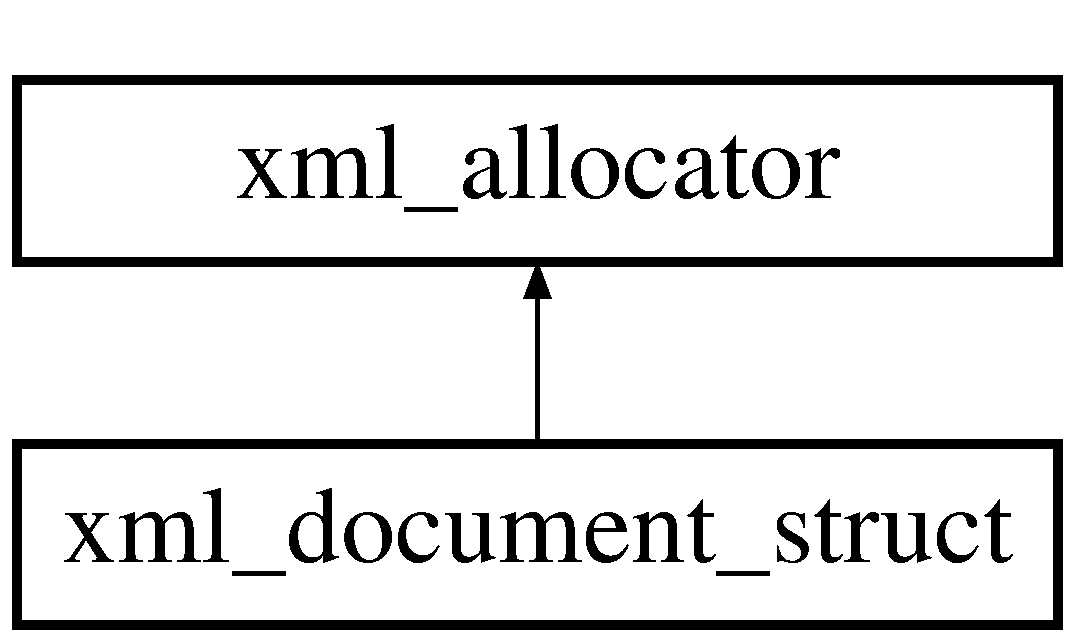
\includegraphics[height=2.000000cm]{structxml__allocator}
\end{center}
\end{figure}
\subsection*{Public Member Functions}
\begin{DoxyCompactItemize}
\item 
\hyperlink{structxml__allocator_ad41b1a18595953aa71a470b45921c0fd}{xml\-\_\-allocator} (\hyperlink{structxml__memory__page}{xml\-\_\-memory\-\_\-page} $\ast$root)
\item 
\hyperlink{structxml__memory__page}{xml\-\_\-memory\-\_\-page} $\ast$ \hyperlink{structxml__allocator_a4b399b01e530220ec5849b912b84063b}{allocate\-\_\-page} (size\-\_\-t data\-\_\-size)
\item 
void $\ast$ \hyperlink{structxml__allocator_a30bb557bc040de54c041c6d3dca6772e}{allocate\-\_\-memory\-\_\-oob} (size\-\_\-t size, \hyperlink{structxml__memory__page}{xml\-\_\-memory\-\_\-page} $\ast$\&out\-\_\-page)
\item 
void $\ast$ \hyperlink{structxml__allocator_afac0b9fac2c2962972f60d0346eb4f39}{allocate\-\_\-memory} (size\-\_\-t size, \hyperlink{structxml__memory__page}{xml\-\_\-memory\-\_\-page} $\ast$\&out\-\_\-page)
\item 
void \hyperlink{structxml__allocator_a5df417155487cce4e0460b123ac33dc6}{deallocate\-\_\-memory} (void $\ast$ptr, size\-\_\-t size, \hyperlink{structxml__memory__page}{xml\-\_\-memory\-\_\-page} $\ast$page)
\item 
char\-\_\-t $\ast$ \hyperlink{structxml__allocator_ac5ec2b5d41672d6494a2742e95e525b3}{allocate\-\_\-string} (size\-\_\-t length)
\item 
void \hyperlink{structxml__allocator_af32c538db4d562c2d0bfe15f7c0aa879}{deallocate\-\_\-string} (char\-\_\-t $\ast$string)
\end{DoxyCompactItemize}
\subsection*{Static Public Member Functions}
\begin{DoxyCompactItemize}
\item 
static void \hyperlink{structxml__allocator_a1c6bfe15a257a094f55659f8d71c209e}{deallocate\-\_\-page} (\hyperlink{structxml__memory__page}{xml\-\_\-memory\-\_\-page} $\ast$page)
\end{DoxyCompactItemize}
\subsection*{Data Fields}
\begin{DoxyCompactItemize}
\item 
\hyperlink{structxml__memory__page}{xml\-\_\-memory\-\_\-page} $\ast$ \hyperlink{structxml__allocator_a38082e85b23743620a257f997a00bb69}{\-\_\-root}
\item 
size\-\_\-t \hyperlink{structxml__allocator_a4908b4aaa8cbbc3bf936ab8a938053c0}{\-\_\-busy\-\_\-size}
\end{DoxyCompactItemize}


\subsection{Constructor \& Destructor Documentation}
\hypertarget{structxml__allocator_ad41b1a18595953aa71a470b45921c0fd}{\index{xml\-\_\-allocator@{xml\-\_\-allocator}!xml\-\_\-allocator@{xml\-\_\-allocator}}
\index{xml\-\_\-allocator@{xml\-\_\-allocator}!xml_allocator@{xml\-\_\-allocator}}
\subsubsection[{xml\-\_\-allocator}]{\setlength{\rightskip}{0pt plus 5cm}xml\-\_\-allocator\-::xml\-\_\-allocator (
\begin{DoxyParamCaption}
\item[{{\bf xml\-\_\-memory\-\_\-page} $\ast$}]{root}
\end{DoxyParamCaption}
)\hspace{0.3cm}{\ttfamily [inline]}}}\label{structxml__allocator_ad41b1a18595953aa71a470b45921c0fd}


\subsection{Member Function Documentation}
\hypertarget{structxml__allocator_afac0b9fac2c2962972f60d0346eb4f39}{\index{xml\-\_\-allocator@{xml\-\_\-allocator}!allocate\-\_\-memory@{allocate\-\_\-memory}}
\index{allocate\-\_\-memory@{allocate\-\_\-memory}!xml_allocator@{xml\-\_\-allocator}}
\subsubsection[{allocate\-\_\-memory}]{\setlength{\rightskip}{0pt plus 5cm}void$\ast$ xml\-\_\-allocator\-::allocate\-\_\-memory (
\begin{DoxyParamCaption}
\item[{size\-\_\-t}]{size, }
\item[{{\bf xml\-\_\-memory\-\_\-page} $\ast$\&}]{out\-\_\-page}
\end{DoxyParamCaption}
)\hspace{0.3cm}{\ttfamily [inline]}}}\label{structxml__allocator_afac0b9fac2c2962972f60d0346eb4f39}
\hypertarget{structxml__allocator_a30bb557bc040de54c041c6d3dca6772e}{\index{xml\-\_\-allocator@{xml\-\_\-allocator}!allocate\-\_\-memory\-\_\-oob@{allocate\-\_\-memory\-\_\-oob}}
\index{allocate\-\_\-memory\-\_\-oob@{allocate\-\_\-memory\-\_\-oob}!xml_allocator@{xml\-\_\-allocator}}
\subsubsection[{allocate\-\_\-memory\-\_\-oob}]{\setlength{\rightskip}{0pt plus 5cm}{\bf P\-U\-G\-I\-\_\-\-\_\-\-F\-N\-\_\-\-N\-O\-\_\-\-I\-N\-L\-I\-N\-E} void $\ast$ xml\-\_\-allocator\-::allocate\-\_\-memory\-\_\-oob (
\begin{DoxyParamCaption}
\item[{size\-\_\-t}]{size, }
\item[{{\bf xml\-\_\-memory\-\_\-page} $\ast$\&}]{out\-\_\-page}
\end{DoxyParamCaption}
)}}\label{structxml__allocator_a30bb557bc040de54c041c6d3dca6772e}
\hypertarget{structxml__allocator_a4b399b01e530220ec5849b912b84063b}{\index{xml\-\_\-allocator@{xml\-\_\-allocator}!allocate\-\_\-page@{allocate\-\_\-page}}
\index{allocate\-\_\-page@{allocate\-\_\-page}!xml_allocator@{xml\-\_\-allocator}}
\subsubsection[{allocate\-\_\-page}]{\setlength{\rightskip}{0pt plus 5cm}{\bf xml\-\_\-memory\-\_\-page}$\ast$ xml\-\_\-allocator\-::allocate\-\_\-page (
\begin{DoxyParamCaption}
\item[{size\-\_\-t}]{data\-\_\-size}
\end{DoxyParamCaption}
)\hspace{0.3cm}{\ttfamily [inline]}}}\label{structxml__allocator_a4b399b01e530220ec5849b912b84063b}
\hypertarget{structxml__allocator_ac5ec2b5d41672d6494a2742e95e525b3}{\index{xml\-\_\-allocator@{xml\-\_\-allocator}!allocate\-\_\-string@{allocate\-\_\-string}}
\index{allocate\-\_\-string@{allocate\-\_\-string}!xml_allocator@{xml\-\_\-allocator}}
\subsubsection[{allocate\-\_\-string}]{\setlength{\rightskip}{0pt plus 5cm}char\-\_\-t$\ast$ xml\-\_\-allocator\-::allocate\-\_\-string (
\begin{DoxyParamCaption}
\item[{size\-\_\-t}]{length}
\end{DoxyParamCaption}
)\hspace{0.3cm}{\ttfamily [inline]}}}\label{structxml__allocator_ac5ec2b5d41672d6494a2742e95e525b3}
\hypertarget{structxml__allocator_a5df417155487cce4e0460b123ac33dc6}{\index{xml\-\_\-allocator@{xml\-\_\-allocator}!deallocate\-\_\-memory@{deallocate\-\_\-memory}}
\index{deallocate\-\_\-memory@{deallocate\-\_\-memory}!xml_allocator@{xml\-\_\-allocator}}
\subsubsection[{deallocate\-\_\-memory}]{\setlength{\rightskip}{0pt plus 5cm}void xml\-\_\-allocator\-::deallocate\-\_\-memory (
\begin{DoxyParamCaption}
\item[{void $\ast$}]{ptr, }
\item[{size\-\_\-t}]{size, }
\item[{{\bf xml\-\_\-memory\-\_\-page} $\ast$}]{page}
\end{DoxyParamCaption}
)\hspace{0.3cm}{\ttfamily [inline]}}}\label{structxml__allocator_a5df417155487cce4e0460b123ac33dc6}
\hypertarget{structxml__allocator_a1c6bfe15a257a094f55659f8d71c209e}{\index{xml\-\_\-allocator@{xml\-\_\-allocator}!deallocate\-\_\-page@{deallocate\-\_\-page}}
\index{deallocate\-\_\-page@{deallocate\-\_\-page}!xml_allocator@{xml\-\_\-allocator}}
\subsubsection[{deallocate\-\_\-page}]{\setlength{\rightskip}{0pt plus 5cm}static void xml\-\_\-allocator\-::deallocate\-\_\-page (
\begin{DoxyParamCaption}
\item[{{\bf xml\-\_\-memory\-\_\-page} $\ast$}]{page}
\end{DoxyParamCaption}
)\hspace{0.3cm}{\ttfamily [inline]}, {\ttfamily [static]}}}\label{structxml__allocator_a1c6bfe15a257a094f55659f8d71c209e}
\hypertarget{structxml__allocator_af32c538db4d562c2d0bfe15f7c0aa879}{\index{xml\-\_\-allocator@{xml\-\_\-allocator}!deallocate\-\_\-string@{deallocate\-\_\-string}}
\index{deallocate\-\_\-string@{deallocate\-\_\-string}!xml_allocator@{xml\-\_\-allocator}}
\subsubsection[{deallocate\-\_\-string}]{\setlength{\rightskip}{0pt plus 5cm}void xml\-\_\-allocator\-::deallocate\-\_\-string (
\begin{DoxyParamCaption}
\item[{char\-\_\-t $\ast$}]{string}
\end{DoxyParamCaption}
)\hspace{0.3cm}{\ttfamily [inline]}}}\label{structxml__allocator_af32c538db4d562c2d0bfe15f7c0aa879}


\subsection{Field Documentation}
\hypertarget{structxml__allocator_a4908b4aaa8cbbc3bf936ab8a938053c0}{\index{xml\-\_\-allocator@{xml\-\_\-allocator}!\-\_\-busy\-\_\-size@{\-\_\-busy\-\_\-size}}
\index{\-\_\-busy\-\_\-size@{\-\_\-busy\-\_\-size}!xml_allocator@{xml\-\_\-allocator}}
\subsubsection[{\-\_\-busy\-\_\-size}]{\setlength{\rightskip}{0pt plus 5cm}size\-\_\-t xml\-\_\-allocator\-::\-\_\-busy\-\_\-size}}\label{structxml__allocator_a4908b4aaa8cbbc3bf936ab8a938053c0}
\hypertarget{structxml__allocator_a38082e85b23743620a257f997a00bb69}{\index{xml\-\_\-allocator@{xml\-\_\-allocator}!\-\_\-root@{\-\_\-root}}
\index{\-\_\-root@{\-\_\-root}!xml_allocator@{xml\-\_\-allocator}}
\subsubsection[{\-\_\-root}]{\setlength{\rightskip}{0pt plus 5cm}{\bf xml\-\_\-memory\-\_\-page}$\ast$ xml\-\_\-allocator\-::\-\_\-root}}\label{structxml__allocator_a38082e85b23743620a257f997a00bb69}


The documentation for this struct was generated from the following file\-:\begin{DoxyCompactItemize}
\item 
System/\hyperlink{pugixml_8cpp}{pugixml.\-cpp}\end{DoxyCompactItemize}

\hypertarget{structpugi_1_1xml__attribute__struct}{
\section{pugi::xml\_\-attribute\_\-struct Struct Reference}
\label{structpugi_1_1xml__attribute__struct}\index{pugi::xml_attribute_struct@{pugi::xml\_\-attribute\_\-struct}}
}
A 'name=value' XML attribute structure.  


\subsection*{Public Member Functions}
\begin{CompactItemize}
\item 
\hyperlink{structpugi_1_1xml__attribute__struct_57bb21cb72613e746a659efdd6425b94}{xml\_\-attribute\_\-struct} (impl::xml\_\-memory\_\-page $\ast$page)
\begin{CompactList}\small\item\em Default ctor. \item\end{CompactList}\end{CompactItemize}
\subsection*{Data Fields}
\begin{CompactItemize}
\item 
uintptr\_\-t \hyperlink{structpugi_1_1xml__attribute__struct_0dca6ca6c129bbf87a7ebaf87f3e12de}{header}
\item 
char\_\-t $\ast$ \hyperlink{structpugi_1_1xml__attribute__struct_a886c4aae23a132e1704717721ee2c19}{name}
\begin{CompactList}\small\item\em Pointer to attribute name. \item\end{CompactList}\item 
char\_\-t $\ast$ \hyperlink{structpugi_1_1xml__attribute__struct_e652627d56cb9dcc0afdd1fbf6570364}{value}
\begin{CompactList}\small\item\em Pointer to attribute value. \item\end{CompactList}\item 
\hyperlink{structpugi_1_1xml__attribute__struct}{xml\_\-attribute\_\-struct} $\ast$ \hyperlink{structpugi_1_1xml__attribute__struct_0e3a022235b316e4cfc1034ceb7d7862}{prev\_\-attribute\_\-c}
\begin{CompactList}\small\item\em Previous attribute (cyclic list). \item\end{CompactList}\item 
\hyperlink{structpugi_1_1xml__attribute__struct}{xml\_\-attribute\_\-struct} $\ast$ \hyperlink{structpugi_1_1xml__attribute__struct_9860c0eb7fa72dc9b69ee9b0575f9efc}{next\_\-attribute}
\begin{CompactList}\small\item\em Next attribute. \item\end{CompactList}\end{CompactItemize}


\subsection{Detailed Description}
A 'name=value' XML attribute structure. 



\subsection{Constructor \& Destructor Documentation}
\hypertarget{structpugi_1_1xml__attribute__struct_57bb21cb72613e746a659efdd6425b94}{
\index{pugi::xml_attribute_struct@{pugi::xml\_\-attribute\_\-struct}!xml_attribute_struct@{xml\_\-attribute\_\-struct}}
\index{xml_attribute_struct@{xml\_\-attribute\_\-struct}!pugi::xml_attribute_struct@{pugi::xml\_\-attribute\_\-struct}}
\subsubsection[xml\_\-attribute\_\-struct]{\setlength{\rightskip}{0pt plus 5cm}pugi::xml\_\-attribute\_\-struct::xml\_\-attribute\_\-struct (impl::xml\_\-memory\_\-page $\ast$ {\em page})\hspace{0.3cm}{\tt  \mbox{[}inline\mbox{]}}}}
\label{structpugi_1_1xml__attribute__struct_57bb21cb72613e746a659efdd6425b94}


Default ctor. 



\subsection{Field Documentation}
\hypertarget{structpugi_1_1xml__attribute__struct_0dca6ca6c129bbf87a7ebaf87f3e12de}{
\index{pugi::xml_attribute_struct@{pugi::xml\_\-attribute\_\-struct}!header@{header}}
\index{header@{header}!pugi::xml_attribute_struct@{pugi::xml\_\-attribute\_\-struct}}
\subsubsection[header]{\setlength{\rightskip}{0pt plus 5cm}uintptr\_\-t \hyperlink{structpugi_1_1xml__attribute__struct_0dca6ca6c129bbf87a7ebaf87f3e12de}{pugi::xml\_\-attribute\_\-struct::header}}}
\label{structpugi_1_1xml__attribute__struct_0dca6ca6c129bbf87a7ebaf87f3e12de}


\hypertarget{structpugi_1_1xml__attribute__struct_a886c4aae23a132e1704717721ee2c19}{
\index{pugi::xml_attribute_struct@{pugi::xml\_\-attribute\_\-struct}!name@{name}}
\index{name@{name}!pugi::xml_attribute_struct@{pugi::xml\_\-attribute\_\-struct}}
\subsubsection[name]{\setlength{\rightskip}{0pt plus 5cm}char\_\-t$\ast$ \hyperlink{structpugi_1_1xml__attribute__struct_a886c4aae23a132e1704717721ee2c19}{pugi::xml\_\-attribute\_\-struct::name}}}
\label{structpugi_1_1xml__attribute__struct_a886c4aae23a132e1704717721ee2c19}


Pointer to attribute name. 

\hypertarget{structpugi_1_1xml__attribute__struct_9860c0eb7fa72dc9b69ee9b0575f9efc}{
\index{pugi::xml_attribute_struct@{pugi::xml\_\-attribute\_\-struct}!next_attribute@{next\_\-attribute}}
\index{next_attribute@{next\_\-attribute}!pugi::xml_attribute_struct@{pugi::xml\_\-attribute\_\-struct}}
\subsubsection[next\_\-attribute]{\setlength{\rightskip}{0pt plus 5cm}\hyperlink{structpugi_1_1xml__attribute__struct}{xml\_\-attribute\_\-struct}$\ast$ \hyperlink{structpugi_1_1xml__attribute__struct_9860c0eb7fa72dc9b69ee9b0575f9efc}{pugi::xml\_\-attribute\_\-struct::next\_\-attribute}}}
\label{structpugi_1_1xml__attribute__struct_9860c0eb7fa72dc9b69ee9b0575f9efc}


Next attribute. 

\hypertarget{structpugi_1_1xml__attribute__struct_0e3a022235b316e4cfc1034ceb7d7862}{
\index{pugi::xml_attribute_struct@{pugi::xml\_\-attribute\_\-struct}!prev_attribute_c@{prev\_\-attribute\_\-c}}
\index{prev_attribute_c@{prev\_\-attribute\_\-c}!pugi::xml_attribute_struct@{pugi::xml\_\-attribute\_\-struct}}
\subsubsection[prev\_\-attribute\_\-c]{\setlength{\rightskip}{0pt plus 5cm}\hyperlink{structpugi_1_1xml__attribute__struct}{xml\_\-attribute\_\-struct}$\ast$ \hyperlink{structpugi_1_1xml__attribute__struct_0e3a022235b316e4cfc1034ceb7d7862}{pugi::xml\_\-attribute\_\-struct::prev\_\-attribute\_\-c}}}
\label{structpugi_1_1xml__attribute__struct_0e3a022235b316e4cfc1034ceb7d7862}


Previous attribute (cyclic list). 

\hypertarget{structpugi_1_1xml__attribute__struct_e652627d56cb9dcc0afdd1fbf6570364}{
\index{pugi::xml_attribute_struct@{pugi::xml\_\-attribute\_\-struct}!value@{value}}
\index{value@{value}!pugi::xml_attribute_struct@{pugi::xml\_\-attribute\_\-struct}}
\subsubsection[value]{\setlength{\rightskip}{0pt plus 5cm}char\_\-t$\ast$ \hyperlink{structpugi_1_1xml__attribute__struct_e652627d56cb9dcc0afdd1fbf6570364}{pugi::xml\_\-attribute\_\-struct::value}}}
\label{structpugi_1_1xml__attribute__struct_e652627d56cb9dcc0afdd1fbf6570364}


Pointer to attribute value. 



The documentation for this struct was generated from the following file:\begin{CompactItemize}
\item 
Utils/\hyperlink{pugixml_8cpp}{pugixml.cpp}\end{CompactItemize}

\hypertarget{classxml__buffered__writer}{
\section{xml\_\-buffered\_\-writer Class Reference}
\label{classxml__buffered__writer}\index{xml_buffered_writer@{xml\_\-buffered\_\-writer}}
}
\subsection*{Public Types}
\begin{CompactItemize}
\item 
\hyperlink{classxml__buffered__writer_e80799461cc7c7c621ff75eb6835e7ce9021e7b22ef17fba93b80380f0ffbbc8}{bufcapacitybytes}
\item 
\hyperlink{classxml__buffered__writer_e80799461cc7c7c621ff75eb6835e7ceb8b49b73105796783607f1f1ddd382cd}{bufcapacity} = bufcapacitybytes / (sizeof(char\_\-t) + 4)
\item 
enum \{ \hyperlink{classxml__buffered__writer_e80799461cc7c7c621ff75eb6835e7ce9021e7b22ef17fba93b80380f0ffbbc8}{bufcapacitybytes}, 
\hyperlink{classxml__buffered__writer_e80799461cc7c7c621ff75eb6835e7ceb8b49b73105796783607f1f1ddd382cd}{bufcapacity} =  bufcapacitybytes / (sizeof(char\_\-t) + 4)
 \}
\end{CompactItemize}
\subsection*{Public Member Functions}
\begin{CompactItemize}
\item 
\hyperlink{classxml__buffered__writer_3c22ad246e2aebb6597935baf4a223a7}{xml\_\-buffered\_\-writer} (xml\_\-writer \&writer\_\-, xml\_\-encoding user\_\-encoding)
\item 
\hyperlink{classxml__buffered__writer_a0aaa7ca5b9b61fb0e9dd79502e8d728}{$\sim$xml\_\-buffered\_\-writer} ()
\item 
void \hyperlink{classxml__buffered__writer_74192d6bbee5ea387377537ede483b4f}{flush} ()
\item 
void \hyperlink{classxml__buffered__writer_a733cb2cd0d5fcacec92c67a7f26c553}{flush} (const char\_\-t $\ast$data, size\_\-t size)
\item 
void \hyperlink{classxml__buffered__writer_f830f04deffd7e28122d8c8973707c94}{write} (const char\_\-t $\ast$data, size\_\-t length)
\item 
void \hyperlink{classxml__buffered__writer_f4181dcf2610619ba4f35d86c3d66372}{write} (const char\_\-t $\ast$data)
\item 
void \hyperlink{classxml__buffered__writer_1aa829bd551a69dd9005d2d46063308f}{write} (char\_\-t d0)
\item 
void \hyperlink{classxml__buffered__writer_4cd6e908908e17c9b07eba34f7317791}{write} (char\_\-t d0, char\_\-t d1)
\item 
void \hyperlink{classxml__buffered__writer_f82b277c1ef5c75d1901bb5a8eb4507f}{write} (char\_\-t d0, char\_\-t d1, char\_\-t d2)
\item 
void \hyperlink{classxml__buffered__writer_f679f459dfa0af257c190b8db57e7dcb}{write} (char\_\-t d0, char\_\-t d1, char\_\-t d2, char\_\-t d3)
\item 
void \hyperlink{classxml__buffered__writer_ad4a4f18223ec3cb1ff607425119b85f}{write} (char\_\-t d0, char\_\-t d1, char\_\-t d2, char\_\-t d3, char\_\-t d4)
\item 
void \hyperlink{classxml__buffered__writer_e6af5067d768c24b9c20422f76737f29}{write} (char\_\-t d0, char\_\-t d1, char\_\-t d2, char\_\-t d3, char\_\-t d4, char\_\-t d5)
\end{CompactItemize}
\subsection*{Data Fields}
\begin{CompactItemize}
\item 
char\_\-t \hyperlink{classxml__buffered__writer_84c87765fbdf444d981ffb0f67899dd4}{buffer} \mbox{[}bufcapacity\mbox{]}
\item 
\begin{tabbing}
xx\=xx\=xx\=xx\=xx\=xx\=xx\=xx\=xx\=\kill
union \{\\
\>uint8\_t \hyperlink{classxml__buffered__writer_c672c70ba0597cf94d35c352ac563891}{data\_u8} \mbox{[}4 $\ast$bufcapacity\mbox{]}\\
\>uint16\_t \hyperlink{classxml__buffered__writer_a969d3724efe221a68927947e3a5196d}{data\_u16} \mbox{[}2 $\ast$bufcapacity\mbox{]}\\
\>uint32\_t \hyperlink{classxml__buffered__writer_fa54826d8227c4ee661e1a9cc1e1acf2}{data\_u32} \mbox{[}bufcapacity\mbox{]}\\
\>char\_t \hyperlink{classxml__buffered__writer_6f21e839a1c66901995c8aae5cc9ad7b}{data\_char} \mbox{[}bufcapacity\mbox{]}\\
\} \hyperlink{classxml__buffered__writer_99e9007c9af7b48a758adb0cbc55a147}{scratch}\\

\end{tabbing}\item 
xml\_\-writer \& \hyperlink{classxml__buffered__writer_37cdd45f867937e1978565f5a0fa318b}{writer}
\item 
size\_\-t \hyperlink{classxml__buffered__writer_6bad6a93035d796939d84bee30e74ce7}{bufsize}
\item 
xml\_\-encoding \hyperlink{classxml__buffered__writer_b810a7286598172e1549561b285f08fb}{encoding}
\end{CompactItemize}
\subsection*{Private Member Functions}
\begin{CompactItemize}
\item 
\hyperlink{classxml__buffered__writer_6ab927cae021733a4b2e9e7cbbb79c13}{xml\_\-buffered\_\-writer} (const \hyperlink{classxml__buffered__writer}{xml\_\-buffered\_\-writer} \&)
\item 
\hyperlink{classxml__buffered__writer}{xml\_\-buffered\_\-writer} \& \hyperlink{classxml__buffered__writer_0aab8cdf0db6269840a0b16319bdb985}{operator=} (const \hyperlink{classxml__buffered__writer}{xml\_\-buffered\_\-writer} \&)
\end{CompactItemize}


\subsection{Member Enumeration Documentation}
\hypertarget{classxml__buffered__writer_e80799461cc7c7c621ff75eb6835e7ce}{
\subsubsection["@4]{\setlength{\rightskip}{0pt plus 5cm}anonymous enum}}
\label{classxml__buffered__writer_e80799461cc7c7c621ff75eb6835e7ce}


\begin{Desc}
\item[Enumerator: ]\par
\begin{description}
\index{bufcapacitybytes@{bufcapacitybytes}!xml_buffered_writer@{xml\_\-buffered\_\-writer}}\index{xml_buffered_writer@{xml\_\-buffered\_\-writer}!bufcapacitybytes@{bufcapacitybytes}}\item[{\em 
\hypertarget{classxml__buffered__writer_e80799461cc7c7c621ff75eb6835e7ce9021e7b22ef17fba93b80380f0ffbbc8}{
bufcapacitybytes}
\label{classxml__buffered__writer_e80799461cc7c7c621ff75eb6835e7ce9021e7b22ef17fba93b80380f0ffbbc8}
}]\index{bufcapacity@{bufcapacity}!xml_buffered_writer@{xml\_\-buffered\_\-writer}}\index{xml_buffered_writer@{xml\_\-buffered\_\-writer}!bufcapacity@{bufcapacity}}\item[{\em 
\hypertarget{classxml__buffered__writer_e80799461cc7c7c621ff75eb6835e7ceb8b49b73105796783607f1f1ddd382cd}{
bufcapacity}
\label{classxml__buffered__writer_e80799461cc7c7c621ff75eb6835e7ceb8b49b73105796783607f1f1ddd382cd}
}]\end{description}
\end{Desc}



\subsection{Constructor \& Destructor Documentation}
\hypertarget{classxml__buffered__writer_6ab927cae021733a4b2e9e7cbbb79c13}{
\index{xml_buffered_writer@{xml\_\-buffered\_\-writer}!xml_buffered_writer@{xml\_\-buffered\_\-writer}}
\index{xml_buffered_writer@{xml\_\-buffered\_\-writer}!xml_buffered_writer@{xml\_\-buffered\_\-writer}}
\subsubsection[xml\_\-buffered\_\-writer]{\setlength{\rightskip}{0pt plus 5cm}xml\_\-buffered\_\-writer::xml\_\-buffered\_\-writer (const \hyperlink{classxml__buffered__writer}{xml\_\-buffered\_\-writer} \&)\hspace{0.3cm}{\tt  \mbox{[}private\mbox{]}}}}
\label{classxml__buffered__writer_6ab927cae021733a4b2e9e7cbbb79c13}


\hypertarget{classxml__buffered__writer_3c22ad246e2aebb6597935baf4a223a7}{
\index{xml_buffered_writer@{xml\_\-buffered\_\-writer}!xml_buffered_writer@{xml\_\-buffered\_\-writer}}
\index{xml_buffered_writer@{xml\_\-buffered\_\-writer}!xml_buffered_writer@{xml\_\-buffered\_\-writer}}
\subsubsection[xml\_\-buffered\_\-writer]{\setlength{\rightskip}{0pt plus 5cm}xml\_\-buffered\_\-writer::xml\_\-buffered\_\-writer (xml\_\-writer \& {\em writer\_\-}, xml\_\-encoding {\em user\_\-encoding})\hspace{0.3cm}{\tt  \mbox{[}inline\mbox{]}}}}
\label{classxml__buffered__writer_3c22ad246e2aebb6597935baf4a223a7}


\hypertarget{classxml__buffered__writer_a0aaa7ca5b9b61fb0e9dd79502e8d728}{
\index{xml_buffered_writer@{xml\_\-buffered\_\-writer}!~xml_buffered_writer@{$\sim$xml\_\-buffered\_\-writer}}
\index{~xml_buffered_writer@{$\sim$xml\_\-buffered\_\-writer}!xml_buffered_writer@{xml\_\-buffered\_\-writer}}
\subsubsection[$\sim$xml\_\-buffered\_\-writer]{\setlength{\rightskip}{0pt plus 5cm}xml\_\-buffered\_\-writer::$\sim$xml\_\-buffered\_\-writer ()\hspace{0.3cm}{\tt  \mbox{[}inline\mbox{]}}}}
\label{classxml__buffered__writer_a0aaa7ca5b9b61fb0e9dd79502e8d728}




\subsection{Member Function Documentation}
\hypertarget{classxml__buffered__writer_a733cb2cd0d5fcacec92c67a7f26c553}{
\index{xml_buffered_writer@{xml\_\-buffered\_\-writer}!flush@{flush}}
\index{flush@{flush}!xml_buffered_writer@{xml\_\-buffered\_\-writer}}
\subsubsection[flush]{\setlength{\rightskip}{0pt plus 5cm}void xml\_\-buffered\_\-writer::flush (const char\_\-t $\ast$ {\em data}, size\_\-t {\em size})\hspace{0.3cm}{\tt  \mbox{[}inline\mbox{]}}}}
\label{classxml__buffered__writer_a733cb2cd0d5fcacec92c67a7f26c553}


\hypertarget{classxml__buffered__writer_74192d6bbee5ea387377537ede483b4f}{
\index{xml_buffered_writer@{xml\_\-buffered\_\-writer}!flush@{flush}}
\index{flush@{flush}!xml_buffered_writer@{xml\_\-buffered\_\-writer}}
\subsubsection[flush]{\setlength{\rightskip}{0pt plus 5cm}void xml\_\-buffered\_\-writer::flush ()\hspace{0.3cm}{\tt  \mbox{[}inline\mbox{]}}}}
\label{classxml__buffered__writer_74192d6bbee5ea387377537ede483b4f}


\hypertarget{classxml__buffered__writer_0aab8cdf0db6269840a0b16319bdb985}{
\index{xml_buffered_writer@{xml\_\-buffered\_\-writer}!operator=@{operator=}}
\index{operator=@{operator=}!xml_buffered_writer@{xml\_\-buffered\_\-writer}}
\subsubsection[operator=]{\setlength{\rightskip}{0pt plus 5cm}\hyperlink{classxml__buffered__writer}{xml\_\-buffered\_\-writer}\& xml\_\-buffered\_\-writer::operator= (const \hyperlink{classxml__buffered__writer}{xml\_\-buffered\_\-writer} \&)\hspace{0.3cm}{\tt  \mbox{[}private\mbox{]}}}}
\label{classxml__buffered__writer_0aab8cdf0db6269840a0b16319bdb985}


\hypertarget{classxml__buffered__writer_e6af5067d768c24b9c20422f76737f29}{
\index{xml_buffered_writer@{xml\_\-buffered\_\-writer}!write@{write}}
\index{write@{write}!xml_buffered_writer@{xml\_\-buffered\_\-writer}}
\subsubsection[write]{\setlength{\rightskip}{0pt plus 5cm}void xml\_\-buffered\_\-writer::write (char\_\-t {\em d0}, char\_\-t {\em d1}, char\_\-t {\em d2}, char\_\-t {\em d3}, char\_\-t {\em d4}, char\_\-t {\em d5})\hspace{0.3cm}{\tt  \mbox{[}inline\mbox{]}}}}
\label{classxml__buffered__writer_e6af5067d768c24b9c20422f76737f29}


\hypertarget{classxml__buffered__writer_ad4a4f18223ec3cb1ff607425119b85f}{
\index{xml_buffered_writer@{xml\_\-buffered\_\-writer}!write@{write}}
\index{write@{write}!xml_buffered_writer@{xml\_\-buffered\_\-writer}}
\subsubsection[write]{\setlength{\rightskip}{0pt plus 5cm}void xml\_\-buffered\_\-writer::write (char\_\-t {\em d0}, char\_\-t {\em d1}, char\_\-t {\em d2}, char\_\-t {\em d3}, char\_\-t {\em d4})\hspace{0.3cm}{\tt  \mbox{[}inline\mbox{]}}}}
\label{classxml__buffered__writer_ad4a4f18223ec3cb1ff607425119b85f}


\hypertarget{classxml__buffered__writer_f679f459dfa0af257c190b8db57e7dcb}{
\index{xml_buffered_writer@{xml\_\-buffered\_\-writer}!write@{write}}
\index{write@{write}!xml_buffered_writer@{xml\_\-buffered\_\-writer}}
\subsubsection[write]{\setlength{\rightskip}{0pt plus 5cm}void xml\_\-buffered\_\-writer::write (char\_\-t {\em d0}, char\_\-t {\em d1}, char\_\-t {\em d2}, char\_\-t {\em d3})\hspace{0.3cm}{\tt  \mbox{[}inline\mbox{]}}}}
\label{classxml__buffered__writer_f679f459dfa0af257c190b8db57e7dcb}


\hypertarget{classxml__buffered__writer_f82b277c1ef5c75d1901bb5a8eb4507f}{
\index{xml_buffered_writer@{xml\_\-buffered\_\-writer}!write@{write}}
\index{write@{write}!xml_buffered_writer@{xml\_\-buffered\_\-writer}}
\subsubsection[write]{\setlength{\rightskip}{0pt plus 5cm}void xml\_\-buffered\_\-writer::write (char\_\-t {\em d0}, char\_\-t {\em d1}, char\_\-t {\em d2})\hspace{0.3cm}{\tt  \mbox{[}inline\mbox{]}}}}
\label{classxml__buffered__writer_f82b277c1ef5c75d1901bb5a8eb4507f}


\hypertarget{classxml__buffered__writer_4cd6e908908e17c9b07eba34f7317791}{
\index{xml_buffered_writer@{xml\_\-buffered\_\-writer}!write@{write}}
\index{write@{write}!xml_buffered_writer@{xml\_\-buffered\_\-writer}}
\subsubsection[write]{\setlength{\rightskip}{0pt plus 5cm}void xml\_\-buffered\_\-writer::write (char\_\-t {\em d0}, char\_\-t {\em d1})\hspace{0.3cm}{\tt  \mbox{[}inline\mbox{]}}}}
\label{classxml__buffered__writer_4cd6e908908e17c9b07eba34f7317791}


\hypertarget{classxml__buffered__writer_1aa829bd551a69dd9005d2d46063308f}{
\index{xml_buffered_writer@{xml\_\-buffered\_\-writer}!write@{write}}
\index{write@{write}!xml_buffered_writer@{xml\_\-buffered\_\-writer}}
\subsubsection[write]{\setlength{\rightskip}{0pt plus 5cm}void xml\_\-buffered\_\-writer::write (char\_\-t {\em d0})\hspace{0.3cm}{\tt  \mbox{[}inline\mbox{]}}}}
\label{classxml__buffered__writer_1aa829bd551a69dd9005d2d46063308f}


\hypertarget{classxml__buffered__writer_f4181dcf2610619ba4f35d86c3d66372}{
\index{xml_buffered_writer@{xml\_\-buffered\_\-writer}!write@{write}}
\index{write@{write}!xml_buffered_writer@{xml\_\-buffered\_\-writer}}
\subsubsection[write]{\setlength{\rightskip}{0pt plus 5cm}void xml\_\-buffered\_\-writer::write (const char\_\-t $\ast$ {\em data})\hspace{0.3cm}{\tt  \mbox{[}inline\mbox{]}}}}
\label{classxml__buffered__writer_f4181dcf2610619ba4f35d86c3d66372}


\hypertarget{classxml__buffered__writer_f830f04deffd7e28122d8c8973707c94}{
\index{xml_buffered_writer@{xml\_\-buffered\_\-writer}!write@{write}}
\index{write@{write}!xml_buffered_writer@{xml\_\-buffered\_\-writer}}
\subsubsection[write]{\setlength{\rightskip}{0pt plus 5cm}void xml\_\-buffered\_\-writer::write (const char\_\-t $\ast$ {\em data}, size\_\-t {\em length})\hspace{0.3cm}{\tt  \mbox{[}inline\mbox{]}}}}
\label{classxml__buffered__writer_f830f04deffd7e28122d8c8973707c94}




\subsection{Field Documentation}
\hypertarget{classxml__buffered__writer_84c87765fbdf444d981ffb0f67899dd4}{
\index{xml_buffered_writer@{xml\_\-buffered\_\-writer}!buffer@{buffer}}
\index{buffer@{buffer}!xml_buffered_writer@{xml\_\-buffered\_\-writer}}
\subsubsection[buffer]{\setlength{\rightskip}{0pt plus 5cm}char\_\-t \hyperlink{classxml__buffered__writer_84c87765fbdf444d981ffb0f67899dd4}{xml\_\-buffered\_\-writer::buffer}\mbox{[}bufcapacity\mbox{]}}}
\label{classxml__buffered__writer_84c87765fbdf444d981ffb0f67899dd4}


\hypertarget{classxml__buffered__writer_6bad6a93035d796939d84bee30e74ce7}{
\index{xml_buffered_writer@{xml\_\-buffered\_\-writer}!bufsize@{bufsize}}
\index{bufsize@{bufsize}!xml_buffered_writer@{xml\_\-buffered\_\-writer}}
\subsubsection[bufsize]{\setlength{\rightskip}{0pt plus 5cm}size\_\-t \hyperlink{classxml__buffered__writer_6bad6a93035d796939d84bee30e74ce7}{xml\_\-buffered\_\-writer::bufsize}}}
\label{classxml__buffered__writer_6bad6a93035d796939d84bee30e74ce7}


\hypertarget{classxml__buffered__writer_6f21e839a1c66901995c8aae5cc9ad7b}{
\index{xml_buffered_writer@{xml\_\-buffered\_\-writer}!data_char@{data\_\-char}}
\index{data_char@{data\_\-char}!xml_buffered_writer@{xml\_\-buffered\_\-writer}}
\subsubsection[data\_\-char]{\setlength{\rightskip}{0pt plus 5cm}char\_\-t \hyperlink{classxml__buffered__writer_6f21e839a1c66901995c8aae5cc9ad7b}{xml\_\-buffered\_\-writer::data\_\-char}\mbox{[}bufcapacity\mbox{]}}}
\label{classxml__buffered__writer_6f21e839a1c66901995c8aae5cc9ad7b}


\hypertarget{classxml__buffered__writer_a969d3724efe221a68927947e3a5196d}{
\index{xml_buffered_writer@{xml\_\-buffered\_\-writer}!data_u16@{data\_\-u16}}
\index{data_u16@{data\_\-u16}!xml_buffered_writer@{xml\_\-buffered\_\-writer}}
\subsubsection[data\_\-u16]{\setlength{\rightskip}{0pt plus 5cm}uint16\_\-t \hyperlink{classxml__buffered__writer_a969d3724efe221a68927947e3a5196d}{xml\_\-buffered\_\-writer::data\_\-u16}\mbox{[}2 $\ast$bufcapacity\mbox{]}}}
\label{classxml__buffered__writer_a969d3724efe221a68927947e3a5196d}


\hypertarget{classxml__buffered__writer_fa54826d8227c4ee661e1a9cc1e1acf2}{
\index{xml_buffered_writer@{xml\_\-buffered\_\-writer}!data_u32@{data\_\-u32}}
\index{data_u32@{data\_\-u32}!xml_buffered_writer@{xml\_\-buffered\_\-writer}}
\subsubsection[data\_\-u32]{\setlength{\rightskip}{0pt plus 5cm}uint32\_\-t \hyperlink{classxml__buffered__writer_fa54826d8227c4ee661e1a9cc1e1acf2}{xml\_\-buffered\_\-writer::data\_\-u32}\mbox{[}bufcapacity\mbox{]}}}
\label{classxml__buffered__writer_fa54826d8227c4ee661e1a9cc1e1acf2}


\hypertarget{classxml__buffered__writer_c672c70ba0597cf94d35c352ac563891}{
\index{xml_buffered_writer@{xml\_\-buffered\_\-writer}!data_u8@{data\_\-u8}}
\index{data_u8@{data\_\-u8}!xml_buffered_writer@{xml\_\-buffered\_\-writer}}
\subsubsection[data\_\-u8]{\setlength{\rightskip}{0pt plus 5cm}uint8\_\-t \hyperlink{classxml__buffered__writer_c672c70ba0597cf94d35c352ac563891}{xml\_\-buffered\_\-writer::data\_\-u8}\mbox{[}4 $\ast$bufcapacity\mbox{]}}}
\label{classxml__buffered__writer_c672c70ba0597cf94d35c352ac563891}


\hypertarget{classxml__buffered__writer_b810a7286598172e1549561b285f08fb}{
\index{xml_buffered_writer@{xml\_\-buffered\_\-writer}!encoding@{encoding}}
\index{encoding@{encoding}!xml_buffered_writer@{xml\_\-buffered\_\-writer}}
\subsubsection[encoding]{\setlength{\rightskip}{0pt plus 5cm}xml\_\-encoding \hyperlink{classxml__buffered__writer_b810a7286598172e1549561b285f08fb}{xml\_\-buffered\_\-writer::encoding}}}
\label{classxml__buffered__writer_b810a7286598172e1549561b285f08fb}


\hypertarget{classxml__buffered__writer_99e9007c9af7b48a758adb0cbc55a147}{
\index{xml_buffered_writer@{xml\_\-buffered\_\-writer}!scratch@{scratch}}
\index{scratch@{scratch}!xml_buffered_writer@{xml\_\-buffered\_\-writer}}
\subsubsection[scratch]{\setlength{\rightskip}{0pt plus 5cm}union \{ ... \}   \hyperlink{classxml__buffered__writer_99e9007c9af7b48a758adb0cbc55a147}{xml\_\-buffered\_\-writer::scratch}}}
\label{classxml__buffered__writer_99e9007c9af7b48a758adb0cbc55a147}


\hypertarget{classxml__buffered__writer_37cdd45f867937e1978565f5a0fa318b}{
\index{xml_buffered_writer@{xml\_\-buffered\_\-writer}!writer@{writer}}
\index{writer@{writer}!xml_buffered_writer@{xml\_\-buffered\_\-writer}}
\subsubsection[writer]{\setlength{\rightskip}{0pt plus 5cm}xml\_\-writer\& \hyperlink{classxml__buffered__writer_37cdd45f867937e1978565f5a0fa318b}{xml\_\-buffered\_\-writer::writer}}}
\label{classxml__buffered__writer_37cdd45f867937e1978565f5a0fa318b}




The documentation for this class was generated from the following file:\begin{CompactItemize}
\item 
Utils/\hyperlink{pugixml_8cpp}{pugixml.cpp}\end{CompactItemize}

\hypertarget{structxml__document__struct}{
\section{xml\_\-document\_\-struct Struct Reference}
\label{structxml__document__struct}\index{xml_document_struct@{xml\_\-document\_\-struct}}
}
Inheritance diagram for xml\_\-document\_\-struct::\begin{figure}[H]
\begin{center}
\leavevmode
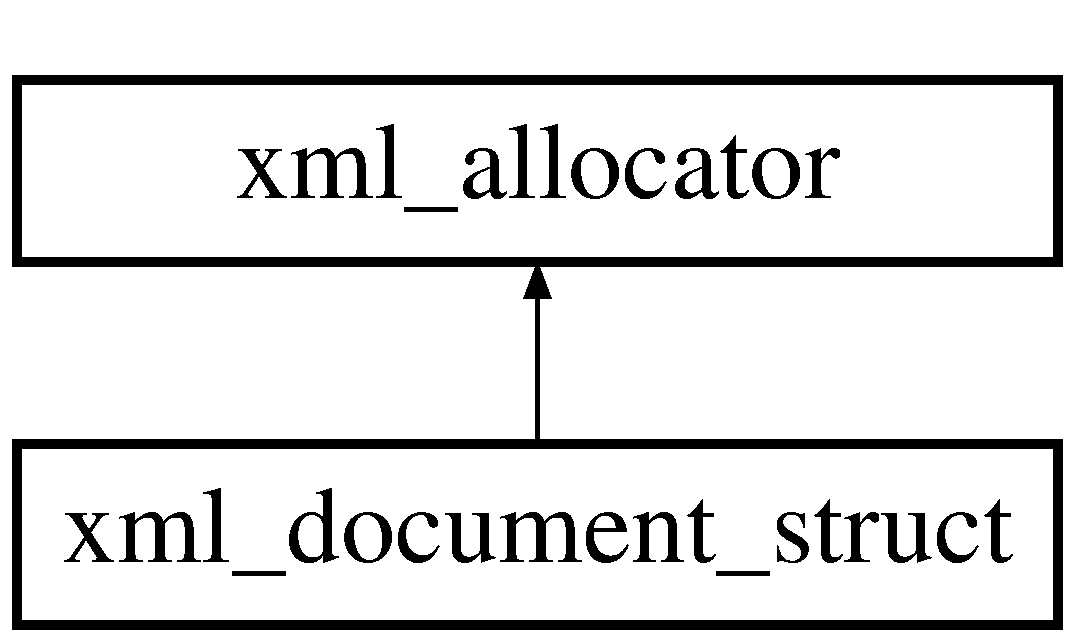
\includegraphics[height=2cm]{structxml__document__struct}
\end{center}
\end{figure}
\subsection*{Public Member Functions}
\begin{CompactItemize}
\item 
\hyperlink{structxml__document__struct_ea3482436c20abd98ca063c3bd5dcfba}{xml\_\-document\_\-struct} (\hyperlink{structxml__memory__page}{xml\_\-memory\_\-page} $\ast$page)
\end{CompactItemize}
\subsection*{Data Fields}
\begin{CompactItemize}
\item 
const char\_\-t $\ast$ \hyperlink{structxml__document__struct_120451f29b8cc2a82a3ecc926449ea0e}{buffer}
\item 
\hyperlink{structxml__extra__buffer}{xml\_\-extra\_\-buffer} $\ast$ \hyperlink{structxml__document__struct_fe3b1efd5b683c306157244496f55c4b}{extra\_\-buffers}
\end{CompactItemize}


\subsection{Constructor \& Destructor Documentation}
\hypertarget{structxml__document__struct_ea3482436c20abd98ca063c3bd5dcfba}{
\index{xml_document_struct@{xml\_\-document\_\-struct}!xml_document_struct@{xml\_\-document\_\-struct}}
\index{xml_document_struct@{xml\_\-document\_\-struct}!xml_document_struct@{xml\_\-document\_\-struct}}
\subsubsection[xml\_\-document\_\-struct]{\setlength{\rightskip}{0pt plus 5cm}xml\_\-document\_\-struct::xml\_\-document\_\-struct (\hyperlink{structxml__memory__page}{xml\_\-memory\_\-page} $\ast$ {\em page})\hspace{0.3cm}{\tt  \mbox{[}inline\mbox{]}}}}
\label{structxml__document__struct_ea3482436c20abd98ca063c3bd5dcfba}




\subsection{Field Documentation}
\hypertarget{structxml__document__struct_120451f29b8cc2a82a3ecc926449ea0e}{
\index{xml_document_struct@{xml\_\-document\_\-struct}!buffer@{buffer}}
\index{buffer@{buffer}!xml_document_struct@{xml\_\-document\_\-struct}}
\subsubsection[buffer]{\setlength{\rightskip}{0pt plus 5cm}const char\_\-t$\ast$ \hyperlink{structxml__document__struct_120451f29b8cc2a82a3ecc926449ea0e}{xml\_\-document\_\-struct::buffer}}}
\label{structxml__document__struct_120451f29b8cc2a82a3ecc926449ea0e}


\hypertarget{structxml__document__struct_fe3b1efd5b683c306157244496f55c4b}{
\index{xml_document_struct@{xml\_\-document\_\-struct}!extra_buffers@{extra\_\-buffers}}
\index{extra_buffers@{extra\_\-buffers}!xml_document_struct@{xml\_\-document\_\-struct}}
\subsubsection[extra\_\-buffers]{\setlength{\rightskip}{0pt plus 5cm}\hyperlink{structxml__extra__buffer}{xml\_\-extra\_\-buffer}$\ast$ \hyperlink{structxml__document__struct_fe3b1efd5b683c306157244496f55c4b}{xml\_\-document\_\-struct::extra\_\-buffers}}}
\label{structxml__document__struct_fe3b1efd5b683c306157244496f55c4b}




The documentation for this struct was generated from the following file:\begin{CompactItemize}
\item 
Utils/\hyperlink{pugixml_8cpp}{pugixml.cpp}\end{CompactItemize}

\hypertarget{structxml__extra__buffer}{
\section{xml\_\-extra\_\-buffer Struct Reference}
\label{structxml__extra__buffer}\index{xml_extra_buffer@{xml\_\-extra\_\-buffer}}
}
\subsection*{Data Fields}
\begin{CompactItemize}
\item 
char\_\-t $\ast$ \hyperlink{structxml__extra__buffer_b24b191b25f92ad4d48009978ebee38c}{buffer}
\item 
\hyperlink{structxml__extra__buffer}{xml\_\-extra\_\-buffer} $\ast$ \hyperlink{structxml__extra__buffer_8aaafa90868ca4d8e06b21eeabd96183}{next}
\end{CompactItemize}


\subsection{Field Documentation}
\hypertarget{structxml__extra__buffer_b24b191b25f92ad4d48009978ebee38c}{
\index{xml_extra_buffer@{xml\_\-extra\_\-buffer}!buffer@{buffer}}
\index{buffer@{buffer}!xml_extra_buffer@{xml\_\-extra\_\-buffer}}
\subsubsection[buffer]{\setlength{\rightskip}{0pt plus 5cm}char\_\-t$\ast$ \hyperlink{structxml__extra__buffer_b24b191b25f92ad4d48009978ebee38c}{xml\_\-extra\_\-buffer::buffer}}}
\label{structxml__extra__buffer_b24b191b25f92ad4d48009978ebee38c}


\hypertarget{structxml__extra__buffer_8aaafa90868ca4d8e06b21eeabd96183}{
\index{xml_extra_buffer@{xml\_\-extra\_\-buffer}!next@{next}}
\index{next@{next}!xml_extra_buffer@{xml\_\-extra\_\-buffer}}
\subsubsection[next]{\setlength{\rightskip}{0pt plus 5cm}\hyperlink{structxml__extra__buffer}{xml\_\-extra\_\-buffer}$\ast$ \hyperlink{structxml__extra__buffer_8aaafa90868ca4d8e06b21eeabd96183}{xml\_\-extra\_\-buffer::next}}}
\label{structxml__extra__buffer_8aaafa90868ca4d8e06b21eeabd96183}




The documentation for this struct was generated from the following file:\begin{CompactItemize}
\item 
Utils/\hyperlink{pugixml_8cpp}{pugixml.cpp}\end{CompactItemize}

\hypertarget{structxml__memory__management__function__storage}{\section{xml\-\_\-memory\-\_\-management\-\_\-function\-\_\-storage$<$ T $>$ Struct Template Reference}
\label{structxml__memory__management__function__storage}\index{xml\-\_\-memory\-\_\-management\-\_\-function\-\_\-storage$<$ T $>$@{xml\-\_\-memory\-\_\-management\-\_\-function\-\_\-storage$<$ T $>$}}
}
\subsection*{Static Public Attributes}
\begin{DoxyCompactItemize}
\item 
static allocation\-\_\-function \hyperlink{structxml__memory__management__function__storage_abb6865f8d07d27fd9273737c59f6e941}{allocate} = \hyperlink{pugixml_8cpp_a5c5a3cf417e46e0b3f5207fb9c6a5c18}{default\-\_\-allocate}
\item 
static deallocation\-\_\-function \hyperlink{structxml__memory__management__function__storage_a1c80a9a045ed6cfb90b17a178e4b3512}{deallocate} = \hyperlink{pugixml_8cpp_a04da64bb4806c0b7491d5d9d73d50100}{default\-\_\-deallocate}
\end{DoxyCompactItemize}


\subsection{Field Documentation}
\hypertarget{structxml__memory__management__function__storage_abb6865f8d07d27fd9273737c59f6e941}{\index{xml\-\_\-memory\-\_\-management\-\_\-function\-\_\-storage@{xml\-\_\-memory\-\_\-management\-\_\-function\-\_\-storage}!allocate@{allocate}}
\index{allocate@{allocate}!xml_memory_management_function_storage@{xml\-\_\-memory\-\_\-management\-\_\-function\-\_\-storage}}
\subsubsection[{allocate}]{\setlength{\rightskip}{0pt plus 5cm}template$<$typename T $>$ allocation\-\_\-function {\bf xml\-\_\-memory\-\_\-management\-\_\-function\-\_\-storage}$<$ T $>$\-::allocate = {\bf default\-\_\-allocate}\hspace{0.3cm}{\ttfamily [static]}}}\label{structxml__memory__management__function__storage_abb6865f8d07d27fd9273737c59f6e941}
\hypertarget{structxml__memory__management__function__storage_a1c80a9a045ed6cfb90b17a178e4b3512}{\index{xml\-\_\-memory\-\_\-management\-\_\-function\-\_\-storage@{xml\-\_\-memory\-\_\-management\-\_\-function\-\_\-storage}!deallocate@{deallocate}}
\index{deallocate@{deallocate}!xml_memory_management_function_storage@{xml\-\_\-memory\-\_\-management\-\_\-function\-\_\-storage}}
\subsubsection[{deallocate}]{\setlength{\rightskip}{0pt plus 5cm}template$<$typename T $>$ deallocation\-\_\-function {\bf xml\-\_\-memory\-\_\-management\-\_\-function\-\_\-storage}$<$ T $>$\-::deallocate = {\bf default\-\_\-deallocate}\hspace{0.3cm}{\ttfamily [static]}}}\label{structxml__memory__management__function__storage_a1c80a9a045ed6cfb90b17a178e4b3512}


The documentation for this struct was generated from the following file\-:\begin{DoxyCompactItemize}
\item 
System/\hyperlink{pugixml_8cpp}{pugixml.\-cpp}\end{DoxyCompactItemize}

\hypertarget{structxml__memory__page}{
\section{xml\_\-memory\_\-page Struct Reference}
\label{structxml__memory__page}\index{xml_memory_page@{xml\_\-memory\_\-page}}
}
\subsection*{Static Public Member Functions}
\begin{CompactItemize}
\item 
static \hyperlink{structxml__memory__page}{xml\_\-memory\_\-page} $\ast$ \hyperlink{structxml__memory__page_b425973f2abb4fa98ff077d88c0df11c}{construct} (void $\ast$\hyperlink{structxml__memory__page_b51315db80e7f2a5afb87c56fedcd734}{memory})
\end{CompactItemize}
\subsection*{Data Fields}
\begin{CompactItemize}
\item 
\hyperlink{structxml__allocator}{xml\_\-allocator} $\ast$ \hyperlink{structxml__memory__page_df8fa143123a842baa59b82fc3d83c3b}{allocator}
\item 
void $\ast$ \hyperlink{structxml__memory__page_b51315db80e7f2a5afb87c56fedcd734}{memory}
\item 
\hyperlink{structxml__memory__page}{xml\_\-memory\_\-page} $\ast$ \hyperlink{structxml__memory__page_014969b0e4a34a6cb24e9823791e60ab}{prev}
\item 
\hyperlink{structxml__memory__page}{xml\_\-memory\_\-page} $\ast$ \hyperlink{structxml__memory__page_326a74e009af80219ea31bc65ed9e45e}{next}
\item 
size\_\-t \hyperlink{structxml__memory__page_04780ddabc14b45baba3d1ded79d355a}{busy\_\-size}
\item 
size\_\-t \hyperlink{structxml__memory__page_b4c29645546530a0e1938b53979890a8}{freed\_\-size}
\item 
char \hyperlink{structxml__memory__page_bd99ed1563aa66fb3573a9208452685c}{data} \mbox{[}1\mbox{]}
\end{CompactItemize}


\subsection{Member Function Documentation}
\hypertarget{structxml__memory__page_b425973f2abb4fa98ff077d88c0df11c}{
\index{xml_memory_page@{xml\_\-memory\_\-page}!construct@{construct}}
\index{construct@{construct}!xml_memory_page@{xml\_\-memory\_\-page}}
\subsubsection[construct]{\setlength{\rightskip}{0pt plus 5cm}static \hyperlink{structxml__memory__page}{xml\_\-memory\_\-page}$\ast$ xml\_\-memory\_\-page::construct (void $\ast$ {\em memory})\hspace{0.3cm}{\tt  \mbox{[}inline, static\mbox{]}}}}
\label{structxml__memory__page_b425973f2abb4fa98ff077d88c0df11c}




\subsection{Field Documentation}
\hypertarget{structxml__memory__page_df8fa143123a842baa59b82fc3d83c3b}{
\index{xml_memory_page@{xml\_\-memory\_\-page}!allocator@{allocator}}
\index{allocator@{allocator}!xml_memory_page@{xml\_\-memory\_\-page}}
\subsubsection[allocator]{\setlength{\rightskip}{0pt plus 5cm}\hyperlink{structxml__allocator}{xml\_\-allocator}$\ast$ \hyperlink{structxml__memory__page_df8fa143123a842baa59b82fc3d83c3b}{xml\_\-memory\_\-page::allocator}}}
\label{structxml__memory__page_df8fa143123a842baa59b82fc3d83c3b}


\hypertarget{structxml__memory__page_04780ddabc14b45baba3d1ded79d355a}{
\index{xml_memory_page@{xml\_\-memory\_\-page}!busy_size@{busy\_\-size}}
\index{busy_size@{busy\_\-size}!xml_memory_page@{xml\_\-memory\_\-page}}
\subsubsection[busy\_\-size]{\setlength{\rightskip}{0pt plus 5cm}size\_\-t \hyperlink{structxml__memory__page_04780ddabc14b45baba3d1ded79d355a}{xml\_\-memory\_\-page::busy\_\-size}}}
\label{structxml__memory__page_04780ddabc14b45baba3d1ded79d355a}


\hypertarget{structxml__memory__page_bd99ed1563aa66fb3573a9208452685c}{
\index{xml_memory_page@{xml\_\-memory\_\-page}!data@{data}}
\index{data@{data}!xml_memory_page@{xml\_\-memory\_\-page}}
\subsubsection[data]{\setlength{\rightskip}{0pt plus 5cm}char \hyperlink{structxml__memory__page_bd99ed1563aa66fb3573a9208452685c}{xml\_\-memory\_\-page::data}\mbox{[}1\mbox{]}}}
\label{structxml__memory__page_bd99ed1563aa66fb3573a9208452685c}


\hypertarget{structxml__memory__page_b4c29645546530a0e1938b53979890a8}{
\index{xml_memory_page@{xml\_\-memory\_\-page}!freed_size@{freed\_\-size}}
\index{freed_size@{freed\_\-size}!xml_memory_page@{xml\_\-memory\_\-page}}
\subsubsection[freed\_\-size]{\setlength{\rightskip}{0pt plus 5cm}size\_\-t \hyperlink{structxml__memory__page_b4c29645546530a0e1938b53979890a8}{xml\_\-memory\_\-page::freed\_\-size}}}
\label{structxml__memory__page_b4c29645546530a0e1938b53979890a8}


\hypertarget{structxml__memory__page_b51315db80e7f2a5afb87c56fedcd734}{
\index{xml_memory_page@{xml\_\-memory\_\-page}!memory@{memory}}
\index{memory@{memory}!xml_memory_page@{xml\_\-memory\_\-page}}
\subsubsection[memory]{\setlength{\rightskip}{0pt plus 5cm}void$\ast$ \hyperlink{structxml__memory__page_b51315db80e7f2a5afb87c56fedcd734}{xml\_\-memory\_\-page::memory}}}
\label{structxml__memory__page_b51315db80e7f2a5afb87c56fedcd734}


\hypertarget{structxml__memory__page_326a74e009af80219ea31bc65ed9e45e}{
\index{xml_memory_page@{xml\_\-memory\_\-page}!next@{next}}
\index{next@{next}!xml_memory_page@{xml\_\-memory\_\-page}}
\subsubsection[next]{\setlength{\rightskip}{0pt plus 5cm}\hyperlink{structxml__memory__page}{xml\_\-memory\_\-page}$\ast$ \hyperlink{structxml__memory__page_326a74e009af80219ea31bc65ed9e45e}{xml\_\-memory\_\-page::next}}}
\label{structxml__memory__page_326a74e009af80219ea31bc65ed9e45e}


\hypertarget{structxml__memory__page_014969b0e4a34a6cb24e9823791e60ab}{
\index{xml_memory_page@{xml\_\-memory\_\-page}!prev@{prev}}
\index{prev@{prev}!xml_memory_page@{xml\_\-memory\_\-page}}
\subsubsection[prev]{\setlength{\rightskip}{0pt plus 5cm}\hyperlink{structxml__memory__page}{xml\_\-memory\_\-page}$\ast$ \hyperlink{structxml__memory__page_014969b0e4a34a6cb24e9823791e60ab}{xml\_\-memory\_\-page::prev}}}
\label{structxml__memory__page_014969b0e4a34a6cb24e9823791e60ab}




The documentation for this struct was generated from the following file:\begin{CompactItemize}
\item 
Utils/\hyperlink{pugixml_8cpp}{pugixml.cpp}\end{CompactItemize}

\hypertarget{structxml__memory__string__header}{
\section{xml\_\-memory\_\-string\_\-header Struct Reference}
\label{structxml__memory__string__header}\index{xml_memory_string_header@{xml\_\-memory\_\-string\_\-header}}
}
\subsection*{Data Fields}
\begin{CompactItemize}
\item 
uint16\_\-t \hyperlink{structxml__memory__string__header_0cc274672f1263f73eeb6bf839bf96ee}{page\_\-offset}
\item 
uint16\_\-t \hyperlink{structxml__memory__string__header_bbb48a709081e6610dffad322499e3f7}{full\_\-size}
\end{CompactItemize}


\subsection{Field Documentation}
\hypertarget{structxml__memory__string__header_bbb48a709081e6610dffad322499e3f7}{
\index{xml_memory_string_header@{xml\_\-memory\_\-string\_\-header}!full_size@{full\_\-size}}
\index{full_size@{full\_\-size}!xml_memory_string_header@{xml\_\-memory\_\-string\_\-header}}
\subsubsection[full\_\-size]{\setlength{\rightskip}{0pt plus 5cm}uint16\_\-t \hyperlink{structxml__memory__string__header_bbb48a709081e6610dffad322499e3f7}{xml\_\-memory\_\-string\_\-header::full\_\-size}}}
\label{structxml__memory__string__header_bbb48a709081e6610dffad322499e3f7}


\hypertarget{structxml__memory__string__header_0cc274672f1263f73eeb6bf839bf96ee}{
\index{xml_memory_string_header@{xml\_\-memory\_\-string\_\-header}!page_offset@{page\_\-offset}}
\index{page_offset@{page\_\-offset}!xml_memory_string_header@{xml\_\-memory\_\-string\_\-header}}
\subsubsection[page\_\-offset]{\setlength{\rightskip}{0pt plus 5cm}uint16\_\-t \hyperlink{structxml__memory__string__header_0cc274672f1263f73eeb6bf839bf96ee}{xml\_\-memory\_\-string\_\-header::page\_\-offset}}}
\label{structxml__memory__string__header_0cc274672f1263f73eeb6bf839bf96ee}




The documentation for this struct was generated from the following file:\begin{CompactItemize}
\item 
Utils/\hyperlink{pugixml_8cpp}{pugixml.cpp}\end{CompactItemize}

\hypertarget{structpugi_1_1xml__node__struct}{\section{pugi\-:\-:xml\-\_\-node\-\_\-struct Struct Reference}
\label{structpugi_1_1xml__node__struct}\index{pugi\-::xml\-\_\-node\-\_\-struct@{pugi\-::xml\-\_\-node\-\_\-struct}}
}


An X\-M\-L document tree node.  


\subsection*{Public Member Functions}
\begin{DoxyCompactItemize}
\item 
\hyperlink{structpugi_1_1xml__node__struct_af9af20f835af8b6b99f9a39c93920ea6}{xml\-\_\-node\-\_\-struct} (impl\-::xml\-\_\-memory\-\_\-page $\ast$page, xml\-\_\-node\-\_\-type type)
\end{DoxyCompactItemize}
\subsection*{Data Fields}
\begin{DoxyCompactItemize}
\item 
uintptr\-\_\-t \hyperlink{structpugi_1_1xml__node__struct_aea2e405a368dc5a278a2d23465f1975c}{header}
\item 
\hyperlink{structpugi_1_1xml__node__struct}{xml\-\_\-node\-\_\-struct} $\ast$ \hyperlink{structpugi_1_1xml__node__struct_af692c222bcc5a9f61108cb3ae0b7b5ea}{parent}
\begin{DoxyCompactList}\small\item\em Pointer to parent. \end{DoxyCompactList}\item 
char\-\_\-t $\ast$ \hyperlink{structpugi_1_1xml__node__struct_ae2324fdbd1e307fb12007d1d0f957a0b}{name}
\begin{DoxyCompactList}\small\item\em Pointer to element name. \end{DoxyCompactList}\item 
char\-\_\-t $\ast$ \hyperlink{structpugi_1_1xml__node__struct_a191e708864fccda17bb66157afdadd2d}{value}
\begin{DoxyCompactList}\small\item\em Pointer to any associated string data. \end{DoxyCompactList}\item 
\hyperlink{structpugi_1_1xml__node__struct}{xml\-\_\-node\-\_\-struct} $\ast$ \hyperlink{structpugi_1_1xml__node__struct_af72c49a0f81928ef664d9d2f0260f23d}{first\-\_\-child}
\begin{DoxyCompactList}\small\item\em First child. \end{DoxyCompactList}\item 
\hyperlink{structpugi_1_1xml__node__struct}{xml\-\_\-node\-\_\-struct} $\ast$ \hyperlink{structpugi_1_1xml__node__struct_a74e62128c88c422c0ed969633bbb2d4e}{prev\-\_\-sibling\-\_\-c}
\begin{DoxyCompactList}\small\item\em Left brother (cyclic list) \end{DoxyCompactList}\item 
\hyperlink{structpugi_1_1xml__node__struct}{xml\-\_\-node\-\_\-struct} $\ast$ \hyperlink{structpugi_1_1xml__node__struct_acf0867e3a77871e37132046d97398a6d}{next\-\_\-sibling}
\begin{DoxyCompactList}\small\item\em Right brother. \end{DoxyCompactList}\item 
\hyperlink{structpugi_1_1xml__attribute__struct}{xml\-\_\-attribute\-\_\-struct} $\ast$ \hyperlink{structpugi_1_1xml__node__struct_a482d2daf97ce0745661cb2c57d8f6fb3}{first\-\_\-attribute}
\begin{DoxyCompactList}\small\item\em First attribute. \end{DoxyCompactList}\end{DoxyCompactItemize}


\subsection{Detailed Description}
An X\-M\-L document tree node. 

\subsection{Constructor \& Destructor Documentation}
\hypertarget{structpugi_1_1xml__node__struct_af9af20f835af8b6b99f9a39c93920ea6}{\index{pugi\-::xml\-\_\-node\-\_\-struct@{pugi\-::xml\-\_\-node\-\_\-struct}!xml\-\_\-node\-\_\-struct@{xml\-\_\-node\-\_\-struct}}
\index{xml\-\_\-node\-\_\-struct@{xml\-\_\-node\-\_\-struct}!pugi::xml_node_struct@{pugi\-::xml\-\_\-node\-\_\-struct}}
\subsubsection[{xml\-\_\-node\-\_\-struct}]{\setlength{\rightskip}{0pt plus 5cm}pugi\-::xml\-\_\-node\-\_\-struct\-::xml\-\_\-node\-\_\-struct (
\begin{DoxyParamCaption}
\item[{impl\-::xml\-\_\-memory\-\_\-page $\ast$}]{page, }
\item[{xml\-\_\-node\-\_\-type}]{type}
\end{DoxyParamCaption}
)\hspace{0.3cm}{\ttfamily [inline]}}}\label{structpugi_1_1xml__node__struct_af9af20f835af8b6b99f9a39c93920ea6}
Default ctor 
\begin{DoxyParams}{Parameters}
{\em type} & -\/ node type \\
\hline
\end{DoxyParams}


\subsection{Field Documentation}
\hypertarget{structpugi_1_1xml__node__struct_a482d2daf97ce0745661cb2c57d8f6fb3}{\index{pugi\-::xml\-\_\-node\-\_\-struct@{pugi\-::xml\-\_\-node\-\_\-struct}!first\-\_\-attribute@{first\-\_\-attribute}}
\index{first\-\_\-attribute@{first\-\_\-attribute}!pugi::xml_node_struct@{pugi\-::xml\-\_\-node\-\_\-struct}}
\subsubsection[{first\-\_\-attribute}]{\setlength{\rightskip}{0pt plus 5cm}{\bf xml\-\_\-attribute\-\_\-struct}$\ast$ pugi\-::xml\-\_\-node\-\_\-struct\-::first\-\_\-attribute}}\label{structpugi_1_1xml__node__struct_a482d2daf97ce0745661cb2c57d8f6fb3}


First attribute. 

\hypertarget{structpugi_1_1xml__node__struct_af72c49a0f81928ef664d9d2f0260f23d}{\index{pugi\-::xml\-\_\-node\-\_\-struct@{pugi\-::xml\-\_\-node\-\_\-struct}!first\-\_\-child@{first\-\_\-child}}
\index{first\-\_\-child@{first\-\_\-child}!pugi::xml_node_struct@{pugi\-::xml\-\_\-node\-\_\-struct}}
\subsubsection[{first\-\_\-child}]{\setlength{\rightskip}{0pt plus 5cm}{\bf xml\-\_\-node\-\_\-struct}$\ast$ pugi\-::xml\-\_\-node\-\_\-struct\-::first\-\_\-child}}\label{structpugi_1_1xml__node__struct_af72c49a0f81928ef664d9d2f0260f23d}


First child. 

\hypertarget{structpugi_1_1xml__node__struct_aea2e405a368dc5a278a2d23465f1975c}{\index{pugi\-::xml\-\_\-node\-\_\-struct@{pugi\-::xml\-\_\-node\-\_\-struct}!header@{header}}
\index{header@{header}!pugi::xml_node_struct@{pugi\-::xml\-\_\-node\-\_\-struct}}
\subsubsection[{header}]{\setlength{\rightskip}{0pt plus 5cm}uintptr\-\_\-t pugi\-::xml\-\_\-node\-\_\-struct\-::header}}\label{structpugi_1_1xml__node__struct_aea2e405a368dc5a278a2d23465f1975c}
\hypertarget{structpugi_1_1xml__node__struct_ae2324fdbd1e307fb12007d1d0f957a0b}{\index{pugi\-::xml\-\_\-node\-\_\-struct@{pugi\-::xml\-\_\-node\-\_\-struct}!name@{name}}
\index{name@{name}!pugi::xml_node_struct@{pugi\-::xml\-\_\-node\-\_\-struct}}
\subsubsection[{name}]{\setlength{\rightskip}{0pt plus 5cm}char\-\_\-t$\ast$ pugi\-::xml\-\_\-node\-\_\-struct\-::name}}\label{structpugi_1_1xml__node__struct_ae2324fdbd1e307fb12007d1d0f957a0b}


Pointer to element name. 

\hypertarget{structpugi_1_1xml__node__struct_acf0867e3a77871e37132046d97398a6d}{\index{pugi\-::xml\-\_\-node\-\_\-struct@{pugi\-::xml\-\_\-node\-\_\-struct}!next\-\_\-sibling@{next\-\_\-sibling}}
\index{next\-\_\-sibling@{next\-\_\-sibling}!pugi::xml_node_struct@{pugi\-::xml\-\_\-node\-\_\-struct}}
\subsubsection[{next\-\_\-sibling}]{\setlength{\rightskip}{0pt plus 5cm}{\bf xml\-\_\-node\-\_\-struct}$\ast$ pugi\-::xml\-\_\-node\-\_\-struct\-::next\-\_\-sibling}}\label{structpugi_1_1xml__node__struct_acf0867e3a77871e37132046d97398a6d}


Right brother. 

\hypertarget{structpugi_1_1xml__node__struct_af692c222bcc5a9f61108cb3ae0b7b5ea}{\index{pugi\-::xml\-\_\-node\-\_\-struct@{pugi\-::xml\-\_\-node\-\_\-struct}!parent@{parent}}
\index{parent@{parent}!pugi::xml_node_struct@{pugi\-::xml\-\_\-node\-\_\-struct}}
\subsubsection[{parent}]{\setlength{\rightskip}{0pt plus 5cm}{\bf xml\-\_\-node\-\_\-struct}$\ast$ pugi\-::xml\-\_\-node\-\_\-struct\-::parent}}\label{structpugi_1_1xml__node__struct_af692c222bcc5a9f61108cb3ae0b7b5ea}


Pointer to parent. 

\hypertarget{structpugi_1_1xml__node__struct_a74e62128c88c422c0ed969633bbb2d4e}{\index{pugi\-::xml\-\_\-node\-\_\-struct@{pugi\-::xml\-\_\-node\-\_\-struct}!prev\-\_\-sibling\-\_\-c@{prev\-\_\-sibling\-\_\-c}}
\index{prev\-\_\-sibling\-\_\-c@{prev\-\_\-sibling\-\_\-c}!pugi::xml_node_struct@{pugi\-::xml\-\_\-node\-\_\-struct}}
\subsubsection[{prev\-\_\-sibling\-\_\-c}]{\setlength{\rightskip}{0pt plus 5cm}{\bf xml\-\_\-node\-\_\-struct}$\ast$ pugi\-::xml\-\_\-node\-\_\-struct\-::prev\-\_\-sibling\-\_\-c}}\label{structpugi_1_1xml__node__struct_a74e62128c88c422c0ed969633bbb2d4e}


Left brother (cyclic list) 

\hypertarget{structpugi_1_1xml__node__struct_a191e708864fccda17bb66157afdadd2d}{\index{pugi\-::xml\-\_\-node\-\_\-struct@{pugi\-::xml\-\_\-node\-\_\-struct}!value@{value}}
\index{value@{value}!pugi::xml_node_struct@{pugi\-::xml\-\_\-node\-\_\-struct}}
\subsubsection[{value}]{\setlength{\rightskip}{0pt plus 5cm}char\-\_\-t$\ast$ pugi\-::xml\-\_\-node\-\_\-struct\-::value}}\label{structpugi_1_1xml__node__struct_a191e708864fccda17bb66157afdadd2d}


Pointer to any associated string data. 



The documentation for this struct was generated from the following file\-:\begin{DoxyCompactItemize}
\item 
System/\hyperlink{pugixml_8cpp}{pugixml.\-cpp}\end{DoxyCompactItemize}

\hypertarget{structxml__parser}{
\section{xml\_\-parser Struct Reference}
\label{structxml__parser}\index{xml_parser@{xml\_\-parser}}
}
\subsection*{Public Member Functions}
\begin{CompactItemize}
\item 
\hyperlink{structxml__parser_cc030c4ed339b238e1ff2d3e6fa7188b}{xml\_\-parser} (const \hyperlink{structxml__allocator}{xml\_\-allocator} \&alloc\_\-)
\item 
char\_\-t $\ast$ \hyperlink{structxml__parser_722853b603ad9a1d1f61bb8115bea5b4}{parse\_\-doctype\_\-primitive} (char\_\-t $\ast$s)
\item 
char\_\-t $\ast$ \hyperlink{structxml__parser_1e996ac9c9993f1939128859596376a1}{parse\_\-doctype\_\-ignore} (char\_\-t $\ast$s)
\item 
char\_\-t $\ast$ \hyperlink{structxml__parser_9bc0e5f3d75cd7edb267a85430e1cdfc}{parse\_\-doctype\_\-group} (char\_\-t $\ast$s, char\_\-t endch, bool toplevel)
\item 
char\_\-t $\ast$ \hyperlink{structxml__parser_40da52e4b27a0a06752930a0edf16fe9}{parse\_\-exclamation} (char\_\-t $\ast$s, xml\_\-node\_\-struct $\ast$cursor, unsigned int optmsk, char\_\-t endch)
\item 
char\_\-t $\ast$ \hyperlink{structxml__parser_2b0edc4fbf2ff448b4d5b31593c5c4fd}{parse\_\-question} (char\_\-t $\ast$s, xml\_\-node\_\-struct $\ast$\&ref\_\-cursor, unsigned int optmsk, char\_\-t endch)
\item 
char\_\-t $\ast$ \hyperlink{structxml__parser_96e76ebea8834b3e56e1c8646e593da4}{parse\_\-tree} (char\_\-t $\ast$s, xml\_\-node\_\-struct $\ast$root, unsigned int optmsk, char\_\-t endch)
\end{CompactItemize}
\subsection*{Static Public Member Functions}
\begin{CompactItemize}
\item 
static char\_\-t $\ast$ \hyperlink{structxml__parser_f0a3f5a488b05da9fa2c87e1dd1f9eda}{parse\_\-skip\_\-bom} (char\_\-t $\ast$s)
\item 
static bool \hyperlink{structxml__parser_6be4da5b3206913d0e3bd8320394df41}{has\_\-element\_\-node\_\-siblings} (xml\_\-node\_\-struct $\ast$node)
\item 
static xml\_\-parse\_\-result \hyperlink{structxml__parser_4bf0acd166edf3fc6cc9543002ff6f5d}{parse} (char\_\-t $\ast$buffer, size\_\-t length, \hyperlink{structxml__document__struct}{xml\_\-document\_\-struct} $\ast$xmldoc, xml\_\-node\_\-struct $\ast$root, unsigned int optmsk)
\end{CompactItemize}
\subsection*{Data Fields}
\begin{CompactItemize}
\item 
\hyperlink{structxml__allocator}{xml\_\-allocator} \hyperlink{structxml__parser_213cf019cbf45f5049acdcae296a2976}{alloc}
\item 
char\_\-t $\ast$ \hyperlink{structxml__parser_2476a71cd7e67b3f4bdbcd1323524503}{error\_\-offset}
\item 
xml\_\-parse\_\-status \hyperlink{structxml__parser_0555859911674e5a7a349447d6533383}{error\_\-status}
\end{CompactItemize}


\subsection{Constructor \& Destructor Documentation}
\hypertarget{structxml__parser_cc030c4ed339b238e1ff2d3e6fa7188b}{
\index{xml_parser@{xml\_\-parser}!xml_parser@{xml\_\-parser}}
\index{xml_parser@{xml\_\-parser}!xml_parser@{xml\_\-parser}}
\subsubsection[xml\_\-parser]{\setlength{\rightskip}{0pt plus 5cm}xml\_\-parser::xml\_\-parser (const \hyperlink{structxml__allocator}{xml\_\-allocator} \& {\em alloc\_\-})\hspace{0.3cm}{\tt  \mbox{[}inline\mbox{]}}}}
\label{structxml__parser_cc030c4ed339b238e1ff2d3e6fa7188b}




\subsection{Member Function Documentation}
\hypertarget{structxml__parser_6be4da5b3206913d0e3bd8320394df41}{
\index{xml_parser@{xml\_\-parser}!has_element_node_siblings@{has\_\-element\_\-node\_\-siblings}}
\index{has_element_node_siblings@{has\_\-element\_\-node\_\-siblings}!xml_parser@{xml\_\-parser}}
\subsubsection[has\_\-element\_\-node\_\-siblings]{\setlength{\rightskip}{0pt plus 5cm}static bool xml\_\-parser::has\_\-element\_\-node\_\-siblings (xml\_\-node\_\-struct $\ast$ {\em node})\hspace{0.3cm}{\tt  \mbox{[}inline, static\mbox{]}}}}
\label{structxml__parser_6be4da5b3206913d0e3bd8320394df41}


\hypertarget{structxml__parser_4bf0acd166edf3fc6cc9543002ff6f5d}{
\index{xml_parser@{xml\_\-parser}!parse@{parse}}
\index{parse@{parse}!xml_parser@{xml\_\-parser}}
\subsubsection[parse]{\setlength{\rightskip}{0pt plus 5cm}static xml\_\-parse\_\-result xml\_\-parser::parse (char\_\-t $\ast$ {\em buffer}, size\_\-t {\em length}, \hyperlink{structxml__document__struct}{xml\_\-document\_\-struct} $\ast$ {\em xmldoc}, xml\_\-node\_\-struct $\ast$ {\em root}, unsigned int {\em optmsk})\hspace{0.3cm}{\tt  \mbox{[}inline, static\mbox{]}}}}
\label{structxml__parser_4bf0acd166edf3fc6cc9543002ff6f5d}


\hypertarget{structxml__parser_9bc0e5f3d75cd7edb267a85430e1cdfc}{
\index{xml_parser@{xml\_\-parser}!parse_doctype_group@{parse\_\-doctype\_\-group}}
\index{parse_doctype_group@{parse\_\-doctype\_\-group}!xml_parser@{xml\_\-parser}}
\subsubsection[parse\_\-doctype\_\-group]{\setlength{\rightskip}{0pt plus 5cm}char\_\-t$\ast$ xml\_\-parser::parse\_\-doctype\_\-group (char\_\-t $\ast$ {\em s}, char\_\-t {\em endch}, bool {\em toplevel})\hspace{0.3cm}{\tt  \mbox{[}inline\mbox{]}}}}
\label{structxml__parser_9bc0e5f3d75cd7edb267a85430e1cdfc}


\hypertarget{structxml__parser_1e996ac9c9993f1939128859596376a1}{
\index{xml_parser@{xml\_\-parser}!parse_doctype_ignore@{parse\_\-doctype\_\-ignore}}
\index{parse_doctype_ignore@{parse\_\-doctype\_\-ignore}!xml_parser@{xml\_\-parser}}
\subsubsection[parse\_\-doctype\_\-ignore]{\setlength{\rightskip}{0pt plus 5cm}char\_\-t$\ast$ xml\_\-parser::parse\_\-doctype\_\-ignore (char\_\-t $\ast$ {\em s})\hspace{0.3cm}{\tt  \mbox{[}inline\mbox{]}}}}
\label{structxml__parser_1e996ac9c9993f1939128859596376a1}


\hypertarget{structxml__parser_722853b603ad9a1d1f61bb8115bea5b4}{
\index{xml_parser@{xml\_\-parser}!parse_doctype_primitive@{parse\_\-doctype\_\-primitive}}
\index{parse_doctype_primitive@{parse\_\-doctype\_\-primitive}!xml_parser@{xml\_\-parser}}
\subsubsection[parse\_\-doctype\_\-primitive]{\setlength{\rightskip}{0pt plus 5cm}char\_\-t$\ast$ xml\_\-parser::parse\_\-doctype\_\-primitive (char\_\-t $\ast$ {\em s})\hspace{0.3cm}{\tt  \mbox{[}inline\mbox{]}}}}
\label{structxml__parser_722853b603ad9a1d1f61bb8115bea5b4}


\hypertarget{structxml__parser_40da52e4b27a0a06752930a0edf16fe9}{
\index{xml_parser@{xml\_\-parser}!parse_exclamation@{parse\_\-exclamation}}
\index{parse_exclamation@{parse\_\-exclamation}!xml_parser@{xml\_\-parser}}
\subsubsection[parse\_\-exclamation]{\setlength{\rightskip}{0pt plus 5cm}char\_\-t$\ast$ xml\_\-parser::parse\_\-exclamation (char\_\-t $\ast$ {\em s}, xml\_\-node\_\-struct $\ast$ {\em cursor}, unsigned int {\em optmsk}, char\_\-t {\em endch})\hspace{0.3cm}{\tt  \mbox{[}inline\mbox{]}}}}
\label{structxml__parser_40da52e4b27a0a06752930a0edf16fe9}


\hypertarget{structxml__parser_2b0edc4fbf2ff448b4d5b31593c5c4fd}{
\index{xml_parser@{xml\_\-parser}!parse_question@{parse\_\-question}}
\index{parse_question@{parse\_\-question}!xml_parser@{xml\_\-parser}}
\subsubsection[parse\_\-question]{\setlength{\rightskip}{0pt plus 5cm}char\_\-t$\ast$ xml\_\-parser::parse\_\-question (char\_\-t $\ast$ {\em s}, xml\_\-node\_\-struct $\ast$\& {\em ref\_\-cursor}, unsigned int {\em optmsk}, char\_\-t {\em endch})\hspace{0.3cm}{\tt  \mbox{[}inline\mbox{]}}}}
\label{structxml__parser_2b0edc4fbf2ff448b4d5b31593c5c4fd}


\hypertarget{structxml__parser_f0a3f5a488b05da9fa2c87e1dd1f9eda}{
\index{xml_parser@{xml\_\-parser}!parse_skip_bom@{parse\_\-skip\_\-bom}}
\index{parse_skip_bom@{parse\_\-skip\_\-bom}!xml_parser@{xml\_\-parser}}
\subsubsection[parse\_\-skip\_\-bom]{\setlength{\rightskip}{0pt plus 5cm}static char\_\-t$\ast$ xml\_\-parser::parse\_\-skip\_\-bom (char\_\-t $\ast$ {\em s})\hspace{0.3cm}{\tt  \mbox{[}inline, static\mbox{]}}}}
\label{structxml__parser_f0a3f5a488b05da9fa2c87e1dd1f9eda}


\hypertarget{structxml__parser_96e76ebea8834b3e56e1c8646e593da4}{
\index{xml_parser@{xml\_\-parser}!parse_tree@{parse\_\-tree}}
\index{parse_tree@{parse\_\-tree}!xml_parser@{xml\_\-parser}}
\subsubsection[parse\_\-tree]{\setlength{\rightskip}{0pt plus 5cm}char\_\-t$\ast$ xml\_\-parser::parse\_\-tree (char\_\-t $\ast$ {\em s}, xml\_\-node\_\-struct $\ast$ {\em root}, unsigned int {\em optmsk}, char\_\-t {\em endch})\hspace{0.3cm}{\tt  \mbox{[}inline\mbox{]}}}}
\label{structxml__parser_96e76ebea8834b3e56e1c8646e593da4}




\subsection{Field Documentation}
\hypertarget{structxml__parser_213cf019cbf45f5049acdcae296a2976}{
\index{xml_parser@{xml\_\-parser}!alloc@{alloc}}
\index{alloc@{alloc}!xml_parser@{xml\_\-parser}}
\subsubsection[alloc]{\setlength{\rightskip}{0pt plus 5cm}\hyperlink{structxml__allocator}{xml\_\-allocator} \hyperlink{structxml__parser_213cf019cbf45f5049acdcae296a2976}{xml\_\-parser::alloc}}}
\label{structxml__parser_213cf019cbf45f5049acdcae296a2976}


\hypertarget{structxml__parser_2476a71cd7e67b3f4bdbcd1323524503}{
\index{xml_parser@{xml\_\-parser}!error_offset@{error\_\-offset}}
\index{error_offset@{error\_\-offset}!xml_parser@{xml\_\-parser}}
\subsubsection[error\_\-offset]{\setlength{\rightskip}{0pt plus 5cm}char\_\-t$\ast$ \hyperlink{structxml__parser_2476a71cd7e67b3f4bdbcd1323524503}{xml\_\-parser::error\_\-offset}}}
\label{structxml__parser_2476a71cd7e67b3f4bdbcd1323524503}


\hypertarget{structxml__parser_0555859911674e5a7a349447d6533383}{
\index{xml_parser@{xml\_\-parser}!error_status@{error\_\-status}}
\index{error_status@{error\_\-status}!xml_parser@{xml\_\-parser}}
\subsubsection[error\_\-status]{\setlength{\rightskip}{0pt plus 5cm}xml\_\-parse\_\-status \hyperlink{structxml__parser_0555859911674e5a7a349447d6533383}{xml\_\-parser::error\_\-status}}}
\label{structxml__parser_0555859911674e5a7a349447d6533383}




The documentation for this struct was generated from the following file:\begin{CompactItemize}
\item 
Utils/\hyperlink{pugixml_8cpp}{pugixml.cpp}\end{CompactItemize}

\hypertarget{structxml__stream__chunk}{
\section{xml\_\-stream\_\-chunk$<$ T $>$ Struct Template Reference}
\label{structxml__stream__chunk}\index{xml_stream_chunk@{xml\_\-stream\_\-chunk}}
}
\subsection*{Public Member Functions}
\begin{CompactItemize}
\item 
\hyperlink{structxml__stream__chunk_8b87fcb2074014dd252f752a95092337}{xml\_\-stream\_\-chunk} ()
\end{CompactItemize}
\subsection*{Static Public Member Functions}
\begin{CompactItemize}
\item 
static \hyperlink{structxml__stream__chunk}{xml\_\-stream\_\-chunk} $\ast$ \hyperlink{structxml__stream__chunk_92cffe33c529ff266329fd4afb59226d}{create} ()
\item 
static void \hyperlink{structxml__stream__chunk_4b812901d59950d48d539e5c8726a0e8}{destroy} (void $\ast$ptr)
\end{CompactItemize}
\subsection*{Data Fields}
\begin{CompactItemize}
\item 
\hyperlink{structxml__stream__chunk}{xml\_\-stream\_\-chunk} $\ast$ \hyperlink{structxml__stream__chunk_d00071f7340adb2bde7c4157d4100b3c}{next}
\item 
size\_\-t \hyperlink{structxml__stream__chunk_42618ba3b7bda1246cfc640149fc34eb}{size}
\item 
T \hyperlink{structxml__stream__chunk_365e2e228a0277467b25a0fea42b8518}{data} \mbox{[}\hyperlink{pugixml_8cpp_a040c77beb7349f7473f072b6dd364b9}{xml\_\-memory\_\-page\_\-size}/sizeof(T)\mbox{]}
\end{CompactItemize}
\subsubsection*{template$<$typename T$>$ struct xml\_\-stream\_\-chunk$<$ T $>$}



\subsection{Constructor \& Destructor Documentation}
\hypertarget{structxml__stream__chunk_8b87fcb2074014dd252f752a95092337}{
\index{xml_stream_chunk@{xml\_\-stream\_\-chunk}!xml_stream_chunk@{xml\_\-stream\_\-chunk}}
\index{xml_stream_chunk@{xml\_\-stream\_\-chunk}!xml_stream_chunk@{xml\_\-stream\_\-chunk}}
\subsubsection[xml\_\-stream\_\-chunk]{\setlength{\rightskip}{0pt plus 5cm}template$<$typename T$>$ \hyperlink{structxml__stream__chunk}{xml\_\-stream\_\-chunk}$<$ T $>$::\hyperlink{structxml__stream__chunk}{xml\_\-stream\_\-chunk} ()\hspace{0.3cm}{\tt  \mbox{[}inline\mbox{]}}}}
\label{structxml__stream__chunk_8b87fcb2074014dd252f752a95092337}




\subsection{Member Function Documentation}
\hypertarget{structxml__stream__chunk_92cffe33c529ff266329fd4afb59226d}{
\index{xml_stream_chunk@{xml\_\-stream\_\-chunk}!create@{create}}
\index{create@{create}!xml_stream_chunk@{xml\_\-stream\_\-chunk}}
\subsubsection[create]{\setlength{\rightskip}{0pt plus 5cm}template$<$typename T$>$ static \hyperlink{structxml__stream__chunk}{xml\_\-stream\_\-chunk}$\ast$ \hyperlink{structxml__stream__chunk}{xml\_\-stream\_\-chunk}$<$ T $>$::create ()\hspace{0.3cm}{\tt  \mbox{[}inline, static\mbox{]}}}}
\label{structxml__stream__chunk_92cffe33c529ff266329fd4afb59226d}


\hypertarget{structxml__stream__chunk_4b812901d59950d48d539e5c8726a0e8}{
\index{xml_stream_chunk@{xml\_\-stream\_\-chunk}!destroy@{destroy}}
\index{destroy@{destroy}!xml_stream_chunk@{xml\_\-stream\_\-chunk}}
\subsubsection[destroy]{\setlength{\rightskip}{0pt plus 5cm}template$<$typename T$>$ static void \hyperlink{structxml__stream__chunk}{xml\_\-stream\_\-chunk}$<$ T $>$::destroy (void $\ast$ {\em ptr})\hspace{0.3cm}{\tt  \mbox{[}inline, static\mbox{]}}}}
\label{structxml__stream__chunk_4b812901d59950d48d539e5c8726a0e8}




\subsection{Field Documentation}
\hypertarget{structxml__stream__chunk_365e2e228a0277467b25a0fea42b8518}{
\index{xml_stream_chunk@{xml\_\-stream\_\-chunk}!data@{data}}
\index{data@{data}!xml_stream_chunk@{xml\_\-stream\_\-chunk}}
\subsubsection[data]{\setlength{\rightskip}{0pt plus 5cm}template$<$typename T$>$ T \hyperlink{structxml__stream__chunk}{xml\_\-stream\_\-chunk}$<$ T $>$::\hyperlink{structxml__stream__chunk_365e2e228a0277467b25a0fea42b8518}{data}\mbox{[}\hyperlink{pugixml_8cpp_a040c77beb7349f7473f072b6dd364b9}{xml\_\-memory\_\-page\_\-size}/sizeof(T)\mbox{]}}}
\label{structxml__stream__chunk_365e2e228a0277467b25a0fea42b8518}


\hypertarget{structxml__stream__chunk_d00071f7340adb2bde7c4157d4100b3c}{
\index{xml_stream_chunk@{xml\_\-stream\_\-chunk}!next@{next}}
\index{next@{next}!xml_stream_chunk@{xml\_\-stream\_\-chunk}}
\subsubsection[next]{\setlength{\rightskip}{0pt plus 5cm}template$<$typename T$>$ \hyperlink{structxml__stream__chunk}{xml\_\-stream\_\-chunk}$\ast$ \hyperlink{structxml__stream__chunk}{xml\_\-stream\_\-chunk}$<$ T $>$::\hyperlink{structxml__stream__chunk_d00071f7340adb2bde7c4157d4100b3c}{next}}}
\label{structxml__stream__chunk_d00071f7340adb2bde7c4157d4100b3c}


\hypertarget{structxml__stream__chunk_42618ba3b7bda1246cfc640149fc34eb}{
\index{xml_stream_chunk@{xml\_\-stream\_\-chunk}!size@{size}}
\index{size@{size}!xml_stream_chunk@{xml\_\-stream\_\-chunk}}
\subsubsection[size]{\setlength{\rightskip}{0pt plus 5cm}template$<$typename T$>$ size\_\-t \hyperlink{structxml__stream__chunk}{xml\_\-stream\_\-chunk}$<$ T $>$::\hyperlink{structxml__stream__chunk_42618ba3b7bda1246cfc640149fc34eb}{size}}}
\label{structxml__stream__chunk_42618ba3b7bda1246cfc640149fc34eb}




The documentation for this struct was generated from the following file:\begin{CompactItemize}
\item 
Utils/\hyperlink{pugixml_8cpp}{pugixml.cpp}\end{CompactItemize}

\hypertarget{classxpath__allocator}{
\section{xpath\_\-allocator Class Reference}
\label{classxpath__allocator}\index{xpath_allocator@{xpath\_\-allocator}}
}
\subsection*{Public Member Functions}
\begin{CompactItemize}
\item 
\hyperlink{classxpath__allocator_3b8ba1722fba115d05949d8f592080e8}{xpath\_\-allocator} (\hyperlink{structxpath__memory__block}{xpath\_\-memory\_\-block} $\ast$root, size\_\-t root\_\-size=0)
\item 
void $\ast$ \hyperlink{classxpath__allocator_a66f3703548657eca5316392a2d79d00}{allocate\_\-nothrow} (size\_\-t size)
\item 
void $\ast$ \hyperlink{classxpath__allocator_ad95aa445f2fdc7c3d1c19b1f3d67cb1}{allocate} (size\_\-t size)
\item 
void $\ast$ \hyperlink{classxpath__allocator_4dd502389202ec8e7420832112a571e5}{reallocate} (void $\ast$ptr, size\_\-t old\_\-size, size\_\-t new\_\-size)
\item 
void \hyperlink{classxpath__allocator_f1c3ec117935d4488bbd16adf807fbc1}{revert} (const \hyperlink{classxpath__allocator}{xpath\_\-allocator} \&state)
\item 
void \hyperlink{classxpath__allocator_9436b8bdef3e0e0ff0df28c2af6a430d}{release} ()
\end{CompactItemize}
\subsection*{Private Attributes}
\begin{CompactItemize}
\item 
\hyperlink{structxpath__memory__block}{xpath\_\-memory\_\-block} $\ast$ \hyperlink{classxpath__allocator_ce647e1e57dd658b4bbcd3b18fb567f1}{\_\-root}
\item 
size\_\-t \hyperlink{classxpath__allocator_dc703a6c3f3a0435f8b5f2e6c770b3fe}{\_\-root\_\-size}
\end{CompactItemize}


\subsection{Constructor \& Destructor Documentation}
\hypertarget{classxpath__allocator_3b8ba1722fba115d05949d8f592080e8}{
\index{xpath_allocator@{xpath\_\-allocator}!xpath_allocator@{xpath\_\-allocator}}
\index{xpath_allocator@{xpath\_\-allocator}!xpath_allocator@{xpath\_\-allocator}}
\subsubsection[xpath\_\-allocator]{\setlength{\rightskip}{0pt plus 5cm}xpath\_\-allocator::xpath\_\-allocator (\hyperlink{structxpath__memory__block}{xpath\_\-memory\_\-block} $\ast$ {\em root}, size\_\-t {\em root\_\-size} = {\tt 0})\hspace{0.3cm}{\tt  \mbox{[}inline\mbox{]}}}}
\label{classxpath__allocator_3b8ba1722fba115d05949d8f592080e8}




\subsection{Member Function Documentation}
\hypertarget{classxpath__allocator_ad95aa445f2fdc7c3d1c19b1f3d67cb1}{
\index{xpath_allocator@{xpath\_\-allocator}!allocate@{allocate}}
\index{allocate@{allocate}!xpath_allocator@{xpath\_\-allocator}}
\subsubsection[allocate]{\setlength{\rightskip}{0pt plus 5cm}void$\ast$ xpath\_\-allocator::allocate (size\_\-t {\em size})\hspace{0.3cm}{\tt  \mbox{[}inline\mbox{]}}}}
\label{classxpath__allocator_ad95aa445f2fdc7c3d1c19b1f3d67cb1}


\hypertarget{classxpath__allocator_a66f3703548657eca5316392a2d79d00}{
\index{xpath_allocator@{xpath\_\-allocator}!allocate_nothrow@{allocate\_\-nothrow}}
\index{allocate_nothrow@{allocate\_\-nothrow}!xpath_allocator@{xpath\_\-allocator}}
\subsubsection[allocate\_\-nothrow]{\setlength{\rightskip}{0pt plus 5cm}void$\ast$ xpath\_\-allocator::allocate\_\-nothrow (size\_\-t {\em size})\hspace{0.3cm}{\tt  \mbox{[}inline\mbox{]}}}}
\label{classxpath__allocator_a66f3703548657eca5316392a2d79d00}


\hypertarget{classxpath__allocator_4dd502389202ec8e7420832112a571e5}{
\index{xpath_allocator@{xpath\_\-allocator}!reallocate@{reallocate}}
\index{reallocate@{reallocate}!xpath_allocator@{xpath\_\-allocator}}
\subsubsection[reallocate]{\setlength{\rightskip}{0pt plus 5cm}void$\ast$ xpath\_\-allocator::reallocate (void $\ast$ {\em ptr}, size\_\-t {\em old\_\-size}, size\_\-t {\em new\_\-size})\hspace{0.3cm}{\tt  \mbox{[}inline\mbox{]}}}}
\label{classxpath__allocator_4dd502389202ec8e7420832112a571e5}


\hypertarget{classxpath__allocator_9436b8bdef3e0e0ff0df28c2af6a430d}{
\index{xpath_allocator@{xpath\_\-allocator}!release@{release}}
\index{release@{release}!xpath_allocator@{xpath\_\-allocator}}
\subsubsection[release]{\setlength{\rightskip}{0pt plus 5cm}void xpath\_\-allocator::release ()\hspace{0.3cm}{\tt  \mbox{[}inline\mbox{]}}}}
\label{classxpath__allocator_9436b8bdef3e0e0ff0df28c2af6a430d}


\hypertarget{classxpath__allocator_f1c3ec117935d4488bbd16adf807fbc1}{
\index{xpath_allocator@{xpath\_\-allocator}!revert@{revert}}
\index{revert@{revert}!xpath_allocator@{xpath\_\-allocator}}
\subsubsection[revert]{\setlength{\rightskip}{0pt plus 5cm}void xpath\_\-allocator::revert (const \hyperlink{classxpath__allocator}{xpath\_\-allocator} \& {\em state})\hspace{0.3cm}{\tt  \mbox{[}inline\mbox{]}}}}
\label{classxpath__allocator_f1c3ec117935d4488bbd16adf807fbc1}




\subsection{Field Documentation}
\hypertarget{classxpath__allocator_ce647e1e57dd658b4bbcd3b18fb567f1}{
\index{xpath_allocator@{xpath\_\-allocator}!_root@{\_\-root}}
\index{_root@{\_\-root}!xpath_allocator@{xpath\_\-allocator}}
\subsubsection[\_\-root]{\setlength{\rightskip}{0pt plus 5cm}\hyperlink{structxpath__memory__block}{xpath\_\-memory\_\-block}$\ast$ \hyperlink{classxpath__allocator_ce647e1e57dd658b4bbcd3b18fb567f1}{xpath\_\-allocator::\_\-root}\hspace{0.3cm}{\tt  \mbox{[}private\mbox{]}}}}
\label{classxpath__allocator_ce647e1e57dd658b4bbcd3b18fb567f1}


\hypertarget{classxpath__allocator_dc703a6c3f3a0435f8b5f2e6c770b3fe}{
\index{xpath_allocator@{xpath\_\-allocator}!_root_size@{\_\-root\_\-size}}
\index{_root_size@{\_\-root\_\-size}!xpath_allocator@{xpath\_\-allocator}}
\subsubsection[\_\-root\_\-size]{\setlength{\rightskip}{0pt plus 5cm}size\_\-t \hyperlink{classxpath__allocator_dc703a6c3f3a0435f8b5f2e6c770b3fe}{xpath\_\-allocator::\_\-root\_\-size}\hspace{0.3cm}{\tt  \mbox{[}private\mbox{]}}}}
\label{classxpath__allocator_dc703a6c3f3a0435f8b5f2e6c770b3fe}




The documentation for this class was generated from the following file:\begin{CompactItemize}
\item 
Utils/\hyperlink{pugixml_8cpp}{pugixml.cpp}\end{CompactItemize}

\hypertarget{structxpath__allocator__capture}{\section{xpath\-\_\-allocator\-\_\-capture Struct Reference}
\label{structxpath__allocator__capture}\index{xpath\-\_\-allocator\-\_\-capture@{xpath\-\_\-allocator\-\_\-capture}}
}
\subsection*{Public Member Functions}
\begin{DoxyCompactItemize}
\item 
\hyperlink{structxpath__allocator__capture_af6925e08c811c0cbda74d4da5b9f2eed}{xpath\-\_\-allocator\-\_\-capture} (\hyperlink{classxpath__allocator}{xpath\-\_\-allocator} $\ast$alloc)
\item 
\hyperlink{structxpath__allocator__capture_a09d4f62de6a543483b94eec405667101}{$\sim$xpath\-\_\-allocator\-\_\-capture} ()
\end{DoxyCompactItemize}
\subsection*{Data Fields}
\begin{DoxyCompactItemize}
\item 
\hyperlink{classxpath__allocator}{xpath\-\_\-allocator} $\ast$ \hyperlink{structxpath__allocator__capture_a382acca931c691699ec84a03fb060cf4}{\-\_\-target}
\item 
\hyperlink{classxpath__allocator}{xpath\-\_\-allocator} \hyperlink{structxpath__allocator__capture_a275859dc99681c12b42ee4f51b713d39}{\-\_\-state}
\end{DoxyCompactItemize}


\subsection{Constructor \& Destructor Documentation}
\hypertarget{structxpath__allocator__capture_af6925e08c811c0cbda74d4da5b9f2eed}{\index{xpath\-\_\-allocator\-\_\-capture@{xpath\-\_\-allocator\-\_\-capture}!xpath\-\_\-allocator\-\_\-capture@{xpath\-\_\-allocator\-\_\-capture}}
\index{xpath\-\_\-allocator\-\_\-capture@{xpath\-\_\-allocator\-\_\-capture}!xpath_allocator_capture@{xpath\-\_\-allocator\-\_\-capture}}
\subsubsection[{xpath\-\_\-allocator\-\_\-capture}]{\setlength{\rightskip}{0pt plus 5cm}xpath\-\_\-allocator\-\_\-capture\-::xpath\-\_\-allocator\-\_\-capture (
\begin{DoxyParamCaption}
\item[{{\bf xpath\-\_\-allocator} $\ast$}]{alloc}
\end{DoxyParamCaption}
)\hspace{0.3cm}{\ttfamily [inline]}}}\label{structxpath__allocator__capture_af6925e08c811c0cbda74d4da5b9f2eed}
\hypertarget{structxpath__allocator__capture_a09d4f62de6a543483b94eec405667101}{\index{xpath\-\_\-allocator\-\_\-capture@{xpath\-\_\-allocator\-\_\-capture}!$\sim$xpath\-\_\-allocator\-\_\-capture@{$\sim$xpath\-\_\-allocator\-\_\-capture}}
\index{$\sim$xpath\-\_\-allocator\-\_\-capture@{$\sim$xpath\-\_\-allocator\-\_\-capture}!xpath_allocator_capture@{xpath\-\_\-allocator\-\_\-capture}}
\subsubsection[{$\sim$xpath\-\_\-allocator\-\_\-capture}]{\setlength{\rightskip}{0pt plus 5cm}xpath\-\_\-allocator\-\_\-capture\-::$\sim$xpath\-\_\-allocator\-\_\-capture (
\begin{DoxyParamCaption}
{}
\end{DoxyParamCaption}
)\hspace{0.3cm}{\ttfamily [inline]}}}\label{structxpath__allocator__capture_a09d4f62de6a543483b94eec405667101}


\subsection{Field Documentation}
\hypertarget{structxpath__allocator__capture_a275859dc99681c12b42ee4f51b713d39}{\index{xpath\-\_\-allocator\-\_\-capture@{xpath\-\_\-allocator\-\_\-capture}!\-\_\-state@{\-\_\-state}}
\index{\-\_\-state@{\-\_\-state}!xpath_allocator_capture@{xpath\-\_\-allocator\-\_\-capture}}
\subsubsection[{\-\_\-state}]{\setlength{\rightskip}{0pt plus 5cm}{\bf xpath\-\_\-allocator} xpath\-\_\-allocator\-\_\-capture\-::\-\_\-state}}\label{structxpath__allocator__capture_a275859dc99681c12b42ee4f51b713d39}
\hypertarget{structxpath__allocator__capture_a382acca931c691699ec84a03fb060cf4}{\index{xpath\-\_\-allocator\-\_\-capture@{xpath\-\_\-allocator\-\_\-capture}!\-\_\-target@{\-\_\-target}}
\index{\-\_\-target@{\-\_\-target}!xpath_allocator_capture@{xpath\-\_\-allocator\-\_\-capture}}
\subsubsection[{\-\_\-target}]{\setlength{\rightskip}{0pt plus 5cm}{\bf xpath\-\_\-allocator}$\ast$ xpath\-\_\-allocator\-\_\-capture\-::\-\_\-target}}\label{structxpath__allocator__capture_a382acca931c691699ec84a03fb060cf4}


The documentation for this struct was generated from the following file\-:\begin{DoxyCompactItemize}
\item 
System/\hyperlink{pugixml_8cpp}{pugixml.\-cpp}\end{DoxyCompactItemize}

\hypertarget{classxpath__ast__node}{\section{xpath\-\_\-ast\-\_\-node Class Reference}
\label{classxpath__ast__node}\index{xpath\-\_\-ast\-\_\-node@{xpath\-\_\-ast\-\_\-node}}
}
\subsection*{Public Member Functions}
\begin{DoxyCompactItemize}
\item 
\hyperlink{classxpath__ast__node_af155d17a4477a693d37f4e34957dcc21}{xpath\-\_\-ast\-\_\-node} (\hyperlink{pugixml_8cpp_a11258a240266b84b6b0526930e5d330d}{ast\-\_\-type\-\_\-t} type, xpath\-\_\-value\-\_\-type rettype\-\_\-, const char\-\_\-t $\ast$value)
\item 
\hyperlink{classxpath__ast__node_ada97458f3fc7d6c87cf70d8084117b0d}{xpath\-\_\-ast\-\_\-node} (\hyperlink{pugixml_8cpp_a11258a240266b84b6b0526930e5d330d}{ast\-\_\-type\-\_\-t} type, xpath\-\_\-value\-\_\-type rettype\-\_\-, double value)
\item 
\hyperlink{classxpath__ast__node_a8de4244f7b9fc7626049197ddc0afab7}{xpath\-\_\-ast\-\_\-node} (\hyperlink{pugixml_8cpp_a11258a240266b84b6b0526930e5d330d}{ast\-\_\-type\-\_\-t} type, xpath\-\_\-value\-\_\-type rettype\-\_\-, xpath\-\_\-variable $\ast$value)
\item 
\hyperlink{classxpath__ast__node_af6f4ffea3f3c7fdb6ef1e759d4b070f4}{xpath\-\_\-ast\-\_\-node} (\hyperlink{pugixml_8cpp_a11258a240266b84b6b0526930e5d330d}{ast\-\_\-type\-\_\-t} type, xpath\-\_\-value\-\_\-type rettype\-\_\-, \hyperlink{classxpath__ast__node}{xpath\-\_\-ast\-\_\-node} $\ast$left=0, \hyperlink{classxpath__ast__node}{xpath\-\_\-ast\-\_\-node} $\ast$right=0)
\item 
\hyperlink{classxpath__ast__node_a7cf74b277deba86a6575796c727fe458}{xpath\-\_\-ast\-\_\-node} (\hyperlink{pugixml_8cpp_a11258a240266b84b6b0526930e5d330d}{ast\-\_\-type\-\_\-t} type, \hyperlink{classxpath__ast__node}{xpath\-\_\-ast\-\_\-node} $\ast$left, \hyperlink{pugixml_8cpp_ae7747145441b0591a5c04f20f6f9189a}{axis\-\_\-t} axis, \hyperlink{pugixml_8cpp_ab268b4264276130baeb17ab629015275}{nodetest\-\_\-t} test, const char\-\_\-t $\ast$contents)
\item 
void \hyperlink{classxpath__ast__node_a2764184d076834284eb3ff3182b845cc}{set\-\_\-next} (\hyperlink{classxpath__ast__node}{xpath\-\_\-ast\-\_\-node} $\ast$value)
\item 
void \hyperlink{classxpath__ast__node_afe044146db852b7d4dbf188fd2ff6c75}{set\-\_\-right} (\hyperlink{classxpath__ast__node}{xpath\-\_\-ast\-\_\-node} $\ast$value)
\item 
bool \hyperlink{classxpath__ast__node_ab7f965a92023bc2704b8e6fd9f3d7c14}{eval\-\_\-boolean} (const \hyperlink{structxpath__context}{xpath\-\_\-context} \&c, const \hyperlink{structxpath__stack}{xpath\-\_\-stack} \&stack)
\item 
double \hyperlink{classxpath__ast__node_a92dd7048e28d486bc7f382d1fc6f1de6}{eval\-\_\-number} (const \hyperlink{structxpath__context}{xpath\-\_\-context} \&c, const \hyperlink{structxpath__stack}{xpath\-\_\-stack} \&stack)
\item 
\hyperlink{classxpath__string}{xpath\-\_\-string} \hyperlink{classxpath__ast__node_aaf931a091af0fb91c25e90b205363b4e}{eval\-\_\-string\-\_\-concat} (const \hyperlink{structxpath__context}{xpath\-\_\-context} \&c, const \hyperlink{structxpath__stack}{xpath\-\_\-stack} \&stack)
\item 
\hyperlink{classxpath__string}{xpath\-\_\-string} \hyperlink{classxpath__ast__node_a6b675237a590548b68d0e0b97518b6df}{eval\-\_\-string} (const \hyperlink{structxpath__context}{xpath\-\_\-context} \&c, const \hyperlink{structxpath__stack}{xpath\-\_\-stack} \&stack)
\item 
\hyperlink{classxpath__node__set__raw}{xpath\-\_\-node\-\_\-set\-\_\-raw} \hyperlink{classxpath__ast__node_a30d98ec97e3129e82ac9ec3f2a759855}{eval\-\_\-node\-\_\-set} (const \hyperlink{structxpath__context}{xpath\-\_\-context} \&c, const \hyperlink{structxpath__stack}{xpath\-\_\-stack} \&stack)
\item 
bool \hyperlink{classxpath__ast__node_a9253f88832441a357ea65639c73a34be}{is\-\_\-posinv} ()
\item 
xpath\-\_\-value\-\_\-type \hyperlink{classxpath__ast__node_a2c3598521141ed4b763fe6c4f852234f}{rettype} () const 
\end{DoxyCompactItemize}
\subsection*{Private Member Functions}
\begin{DoxyCompactItemize}
\item 
\hyperlink{classxpath__ast__node_ae5a059e41b41505bef1f7dbebda8070b}{xpath\-\_\-ast\-\_\-node} (const \hyperlink{classxpath__ast__node}{xpath\-\_\-ast\-\_\-node} \&)
\item 
\hyperlink{classxpath__ast__node}{xpath\-\_\-ast\-\_\-node} \& \hyperlink{classxpath__ast__node_a60fddea92b095c2b8705f12f7309e6aa}{operator=} (const \hyperlink{classxpath__ast__node}{xpath\-\_\-ast\-\_\-node} \&)
\item 
void \hyperlink{classxpath__ast__node_afcefe6b386c214349c5e23f13828fa1e}{apply\-\_\-predicate} (\hyperlink{classxpath__node__set__raw}{xpath\-\_\-node\-\_\-set\-\_\-raw} \&ns, size\-\_\-t first, \hyperlink{classxpath__ast__node}{xpath\-\_\-ast\-\_\-node} $\ast$expr, const \hyperlink{structxpath__stack}{xpath\-\_\-stack} \&stack)
\item 
void \hyperlink{classxpath__ast__node_ae5e3b5fec836d9478ebd195dda7fdedd}{apply\-\_\-predicates} (\hyperlink{classxpath__node__set__raw}{xpath\-\_\-node\-\_\-set\-\_\-raw} \&ns, size\-\_\-t first, const \hyperlink{structxpath__stack}{xpath\-\_\-stack} \&stack)
\item 
void \hyperlink{classxpath__ast__node_aa141bfbd4d5e42da83f0de8f729eb849}{step\-\_\-push} (\hyperlink{classxpath__node__set__raw}{xpath\-\_\-node\-\_\-set\-\_\-raw} \&ns, const xml\-\_\-attribute \&a, const xml\-\_\-node \&parent, \hyperlink{classxpath__allocator}{xpath\-\_\-allocator} $\ast$alloc)
\item 
void \hyperlink{classxpath__ast__node_a7083f1a6c3d4128bb8a4ac147851a86b}{step\-\_\-push} (\hyperlink{classxpath__node__set__raw}{xpath\-\_\-node\-\_\-set\-\_\-raw} \&ns, const xml\-\_\-node \&n, \hyperlink{classxpath__allocator}{xpath\-\_\-allocator} $\ast$alloc)
\item 
{\footnotesize template$<$class T $>$ }\\void \hyperlink{classxpath__ast__node_a725919925f8489f279173c1b653ba092}{step\-\_\-fill} (\hyperlink{classxpath__node__set__raw}{xpath\-\_\-node\-\_\-set\-\_\-raw} \&ns, const xml\-\_\-node \&n, \hyperlink{classxpath__allocator}{xpath\-\_\-allocator} $\ast$alloc, T)
\item 
{\footnotesize template$<$class T $>$ }\\void \hyperlink{classxpath__ast__node_aa65fdd16b494e000821cc2d22de7e2c1}{step\-\_\-fill} (\hyperlink{classxpath__node__set__raw}{xpath\-\_\-node\-\_\-set\-\_\-raw} \&ns, const xml\-\_\-attribute \&a, const xml\-\_\-node \&p, \hyperlink{classxpath__allocator}{xpath\-\_\-allocator} $\ast$alloc, T v)
\item 
{\footnotesize template$<$class T $>$ }\\\hyperlink{classxpath__node__set__raw}{xpath\-\_\-node\-\_\-set\-\_\-raw} \hyperlink{classxpath__ast__node_a80577a0dc3e6369c79958eb9beb2edbc}{step\-\_\-do} (const \hyperlink{structxpath__context}{xpath\-\_\-context} \&c, const \hyperlink{structxpath__stack}{xpath\-\_\-stack} \&stack, T v)
\end{DoxyCompactItemize}
\subsection*{Static Private Member Functions}
\begin{DoxyCompactItemize}
\item 
{\footnotesize template$<$class Comp $>$ }\\static bool \hyperlink{classxpath__ast__node_a98dd7f6e67fe2c56c63056eed835d6a4}{compare\-\_\-eq} (\hyperlink{classxpath__ast__node}{xpath\-\_\-ast\-\_\-node} $\ast$lhs, \hyperlink{classxpath__ast__node}{xpath\-\_\-ast\-\_\-node} $\ast$rhs, const \hyperlink{structxpath__context}{xpath\-\_\-context} \&c, const \hyperlink{structxpath__stack}{xpath\-\_\-stack} \&stack, const Comp \&comp)
\item 
{\footnotesize template$<$class Comp $>$ }\\static bool \hyperlink{classxpath__ast__node_abb6e4c529276eaf882233dbb6e04e111}{compare\-\_\-rel} (\hyperlink{classxpath__ast__node}{xpath\-\_\-ast\-\_\-node} $\ast$lhs, \hyperlink{classxpath__ast__node}{xpath\-\_\-ast\-\_\-node} $\ast$rhs, const \hyperlink{structxpath__context}{xpath\-\_\-context} \&c, const \hyperlink{structxpath__stack}{xpath\-\_\-stack} \&stack, const Comp \&comp)
\end{DoxyCompactItemize}
\subsection*{Private Attributes}
\begin{DoxyCompactItemize}
\item 
char \hyperlink{classxpath__ast__node_ad285f423090a0aaee3c4126da65066d1}{\-\_\-type}
\item 
char \hyperlink{classxpath__ast__node_ab84a640f3a0f00d4d611d8cdd1f5c029}{\-\_\-rettype}
\item 
char \hyperlink{classxpath__ast__node_a97b21db6df156c37ef7f2e6f69478b77}{\-\_\-axis}
\item 
char \hyperlink{classxpath__ast__node_a421f6ed5f666ced9d6fe3692e84d7b89}{\-\_\-test}
\item 
\hyperlink{classxpath__ast__node}{xpath\-\_\-ast\-\_\-node} $\ast$ \hyperlink{classxpath__ast__node_ad229146ced94be21eb5e4921b43a7ebb}{\-\_\-left}
\item 
\hyperlink{classxpath__ast__node}{xpath\-\_\-ast\-\_\-node} $\ast$ \hyperlink{classxpath__ast__node_ab3935ea7e83f4421b20840cd84f0b37d}{\-\_\-right}
\item 
\hyperlink{classxpath__ast__node}{xpath\-\_\-ast\-\_\-node} $\ast$ \hyperlink{classxpath__ast__node_a10059a66ecff3384e175e00d9fa2afcd}{\-\_\-next}
\item 
\begin{tabbing}
xx\=xx\=xx\=xx\=xx\=xx\=xx\=xx\=xx\=\kill
union \{\\
\>const char\_t $\ast$ \hyperlink{classxpath__ast__node_a187822d65799b3bbccd8d0522bd14e59}{string}\\
\>double \hyperlink{classxpath__ast__node_a73870c7a83538e525398855b26154484}{number}\\
\>xpath\_variable $\ast$ \hyperlink{classxpath__ast__node_a0fd3b0d8f930836105eeff6e2efa5ad3}{variable}\\
\>const char\_t $\ast$ \hyperlink{classxpath__ast__node_a50f44079b7f3e399e23488f520a34f17}{nodetest}\\
\} \hyperlink{classxpath__ast__node_a4d08bfca00b137fc5b94314edeed2501}{\_data}\\

\end{tabbing}\end{DoxyCompactItemize}


\subsection{Constructor \& Destructor Documentation}
\hypertarget{classxpath__ast__node_ae5a059e41b41505bef1f7dbebda8070b}{\index{xpath\-\_\-ast\-\_\-node@{xpath\-\_\-ast\-\_\-node}!xpath\-\_\-ast\-\_\-node@{xpath\-\_\-ast\-\_\-node}}
\index{xpath\-\_\-ast\-\_\-node@{xpath\-\_\-ast\-\_\-node}!xpath_ast_node@{xpath\-\_\-ast\-\_\-node}}
\subsubsection[{xpath\-\_\-ast\-\_\-node}]{\setlength{\rightskip}{0pt plus 5cm}xpath\-\_\-ast\-\_\-node\-::xpath\-\_\-ast\-\_\-node (
\begin{DoxyParamCaption}
\item[{const {\bf xpath\-\_\-ast\-\_\-node} \&}]{}
\end{DoxyParamCaption}
)\hspace{0.3cm}{\ttfamily [private]}}}\label{classxpath__ast__node_ae5a059e41b41505bef1f7dbebda8070b}
\hypertarget{classxpath__ast__node_af155d17a4477a693d37f4e34957dcc21}{\index{xpath\-\_\-ast\-\_\-node@{xpath\-\_\-ast\-\_\-node}!xpath\-\_\-ast\-\_\-node@{xpath\-\_\-ast\-\_\-node}}
\index{xpath\-\_\-ast\-\_\-node@{xpath\-\_\-ast\-\_\-node}!xpath_ast_node@{xpath\-\_\-ast\-\_\-node}}
\subsubsection[{xpath\-\_\-ast\-\_\-node}]{\setlength{\rightskip}{0pt plus 5cm}xpath\-\_\-ast\-\_\-node\-::xpath\-\_\-ast\-\_\-node (
\begin{DoxyParamCaption}
\item[{{\bf ast\-\_\-type\-\_\-t}}]{type, }
\item[{xpath\-\_\-value\-\_\-type}]{rettype\-\_\-, }
\item[{const char\-\_\-t $\ast$}]{value}
\end{DoxyParamCaption}
)\hspace{0.3cm}{\ttfamily [inline]}}}\label{classxpath__ast__node_af155d17a4477a693d37f4e34957dcc21}
\hypertarget{classxpath__ast__node_ada97458f3fc7d6c87cf70d8084117b0d}{\index{xpath\-\_\-ast\-\_\-node@{xpath\-\_\-ast\-\_\-node}!xpath\-\_\-ast\-\_\-node@{xpath\-\_\-ast\-\_\-node}}
\index{xpath\-\_\-ast\-\_\-node@{xpath\-\_\-ast\-\_\-node}!xpath_ast_node@{xpath\-\_\-ast\-\_\-node}}
\subsubsection[{xpath\-\_\-ast\-\_\-node}]{\setlength{\rightskip}{0pt plus 5cm}xpath\-\_\-ast\-\_\-node\-::xpath\-\_\-ast\-\_\-node (
\begin{DoxyParamCaption}
\item[{{\bf ast\-\_\-type\-\_\-t}}]{type, }
\item[{xpath\-\_\-value\-\_\-type}]{rettype\-\_\-, }
\item[{double}]{value}
\end{DoxyParamCaption}
)\hspace{0.3cm}{\ttfamily [inline]}}}\label{classxpath__ast__node_ada97458f3fc7d6c87cf70d8084117b0d}
\hypertarget{classxpath__ast__node_a8de4244f7b9fc7626049197ddc0afab7}{\index{xpath\-\_\-ast\-\_\-node@{xpath\-\_\-ast\-\_\-node}!xpath\-\_\-ast\-\_\-node@{xpath\-\_\-ast\-\_\-node}}
\index{xpath\-\_\-ast\-\_\-node@{xpath\-\_\-ast\-\_\-node}!xpath_ast_node@{xpath\-\_\-ast\-\_\-node}}
\subsubsection[{xpath\-\_\-ast\-\_\-node}]{\setlength{\rightskip}{0pt plus 5cm}xpath\-\_\-ast\-\_\-node\-::xpath\-\_\-ast\-\_\-node (
\begin{DoxyParamCaption}
\item[{{\bf ast\-\_\-type\-\_\-t}}]{type, }
\item[{xpath\-\_\-value\-\_\-type}]{rettype\-\_\-, }
\item[{xpath\-\_\-variable $\ast$}]{value}
\end{DoxyParamCaption}
)\hspace{0.3cm}{\ttfamily [inline]}}}\label{classxpath__ast__node_a8de4244f7b9fc7626049197ddc0afab7}
\hypertarget{classxpath__ast__node_af6f4ffea3f3c7fdb6ef1e759d4b070f4}{\index{xpath\-\_\-ast\-\_\-node@{xpath\-\_\-ast\-\_\-node}!xpath\-\_\-ast\-\_\-node@{xpath\-\_\-ast\-\_\-node}}
\index{xpath\-\_\-ast\-\_\-node@{xpath\-\_\-ast\-\_\-node}!xpath_ast_node@{xpath\-\_\-ast\-\_\-node}}
\subsubsection[{xpath\-\_\-ast\-\_\-node}]{\setlength{\rightskip}{0pt plus 5cm}xpath\-\_\-ast\-\_\-node\-::xpath\-\_\-ast\-\_\-node (
\begin{DoxyParamCaption}
\item[{{\bf ast\-\_\-type\-\_\-t}}]{type, }
\item[{xpath\-\_\-value\-\_\-type}]{rettype\-\_\-, }
\item[{{\bf xpath\-\_\-ast\-\_\-node} $\ast$}]{left = {\ttfamily 0}, }
\item[{{\bf xpath\-\_\-ast\-\_\-node} $\ast$}]{right = {\ttfamily 0}}
\end{DoxyParamCaption}
)\hspace{0.3cm}{\ttfamily [inline]}}}\label{classxpath__ast__node_af6f4ffea3f3c7fdb6ef1e759d4b070f4}
\hypertarget{classxpath__ast__node_a7cf74b277deba86a6575796c727fe458}{\index{xpath\-\_\-ast\-\_\-node@{xpath\-\_\-ast\-\_\-node}!xpath\-\_\-ast\-\_\-node@{xpath\-\_\-ast\-\_\-node}}
\index{xpath\-\_\-ast\-\_\-node@{xpath\-\_\-ast\-\_\-node}!xpath_ast_node@{xpath\-\_\-ast\-\_\-node}}
\subsubsection[{xpath\-\_\-ast\-\_\-node}]{\setlength{\rightskip}{0pt plus 5cm}xpath\-\_\-ast\-\_\-node\-::xpath\-\_\-ast\-\_\-node (
\begin{DoxyParamCaption}
\item[{{\bf ast\-\_\-type\-\_\-t}}]{type, }
\item[{{\bf xpath\-\_\-ast\-\_\-node} $\ast$}]{left, }
\item[{{\bf axis\-\_\-t}}]{axis, }
\item[{{\bf nodetest\-\_\-t}}]{test, }
\item[{const char\-\_\-t $\ast$}]{contents}
\end{DoxyParamCaption}
)\hspace{0.3cm}{\ttfamily [inline]}}}\label{classxpath__ast__node_a7cf74b277deba86a6575796c727fe458}


\subsection{Member Function Documentation}
\hypertarget{classxpath__ast__node_afcefe6b386c214349c5e23f13828fa1e}{\index{xpath\-\_\-ast\-\_\-node@{xpath\-\_\-ast\-\_\-node}!apply\-\_\-predicate@{apply\-\_\-predicate}}
\index{apply\-\_\-predicate@{apply\-\_\-predicate}!xpath_ast_node@{xpath\-\_\-ast\-\_\-node}}
\subsubsection[{apply\-\_\-predicate}]{\setlength{\rightskip}{0pt plus 5cm}void xpath\-\_\-ast\-\_\-node\-::apply\-\_\-predicate (
\begin{DoxyParamCaption}
\item[{{\bf xpath\-\_\-node\-\_\-set\-\_\-raw} \&}]{ns, }
\item[{size\-\_\-t}]{first, }
\item[{{\bf xpath\-\_\-ast\-\_\-node} $\ast$}]{expr, }
\item[{const {\bf xpath\-\_\-stack} \&}]{stack}
\end{DoxyParamCaption}
)\hspace{0.3cm}{\ttfamily [inline]}, {\ttfamily [private]}}}\label{classxpath__ast__node_afcefe6b386c214349c5e23f13828fa1e}
\hypertarget{classxpath__ast__node_ae5e3b5fec836d9478ebd195dda7fdedd}{\index{xpath\-\_\-ast\-\_\-node@{xpath\-\_\-ast\-\_\-node}!apply\-\_\-predicates@{apply\-\_\-predicates}}
\index{apply\-\_\-predicates@{apply\-\_\-predicates}!xpath_ast_node@{xpath\-\_\-ast\-\_\-node}}
\subsubsection[{apply\-\_\-predicates}]{\setlength{\rightskip}{0pt plus 5cm}void xpath\-\_\-ast\-\_\-node\-::apply\-\_\-predicates (
\begin{DoxyParamCaption}
\item[{{\bf xpath\-\_\-node\-\_\-set\-\_\-raw} \&}]{ns, }
\item[{size\-\_\-t}]{first, }
\item[{const {\bf xpath\-\_\-stack} \&}]{stack}
\end{DoxyParamCaption}
)\hspace{0.3cm}{\ttfamily [inline]}, {\ttfamily [private]}}}\label{classxpath__ast__node_ae5e3b5fec836d9478ebd195dda7fdedd}
\hypertarget{classxpath__ast__node_a98dd7f6e67fe2c56c63056eed835d6a4}{\index{xpath\-\_\-ast\-\_\-node@{xpath\-\_\-ast\-\_\-node}!compare\-\_\-eq@{compare\-\_\-eq}}
\index{compare\-\_\-eq@{compare\-\_\-eq}!xpath_ast_node@{xpath\-\_\-ast\-\_\-node}}
\subsubsection[{compare\-\_\-eq}]{\setlength{\rightskip}{0pt plus 5cm}template$<$class Comp $>$ static bool xpath\-\_\-ast\-\_\-node\-::compare\-\_\-eq (
\begin{DoxyParamCaption}
\item[{{\bf xpath\-\_\-ast\-\_\-node} $\ast$}]{lhs, }
\item[{{\bf xpath\-\_\-ast\-\_\-node} $\ast$}]{rhs, }
\item[{const {\bf xpath\-\_\-context} \&}]{c, }
\item[{const {\bf xpath\-\_\-stack} \&}]{stack, }
\item[{const Comp \&}]{comp}
\end{DoxyParamCaption}
)\hspace{0.3cm}{\ttfamily [inline]}, {\ttfamily [static]}, {\ttfamily [private]}}}\label{classxpath__ast__node_a98dd7f6e67fe2c56c63056eed835d6a4}
\hypertarget{classxpath__ast__node_abb6e4c529276eaf882233dbb6e04e111}{\index{xpath\-\_\-ast\-\_\-node@{xpath\-\_\-ast\-\_\-node}!compare\-\_\-rel@{compare\-\_\-rel}}
\index{compare\-\_\-rel@{compare\-\_\-rel}!xpath_ast_node@{xpath\-\_\-ast\-\_\-node}}
\subsubsection[{compare\-\_\-rel}]{\setlength{\rightskip}{0pt plus 5cm}template$<$class Comp $>$ static bool xpath\-\_\-ast\-\_\-node\-::compare\-\_\-rel (
\begin{DoxyParamCaption}
\item[{{\bf xpath\-\_\-ast\-\_\-node} $\ast$}]{lhs, }
\item[{{\bf xpath\-\_\-ast\-\_\-node} $\ast$}]{rhs, }
\item[{const {\bf xpath\-\_\-context} \&}]{c, }
\item[{const {\bf xpath\-\_\-stack} \&}]{stack, }
\item[{const Comp \&}]{comp}
\end{DoxyParamCaption}
)\hspace{0.3cm}{\ttfamily [inline]}, {\ttfamily [static]}, {\ttfamily [private]}}}\label{classxpath__ast__node_abb6e4c529276eaf882233dbb6e04e111}
\hypertarget{classxpath__ast__node_ab7f965a92023bc2704b8e6fd9f3d7c14}{\index{xpath\-\_\-ast\-\_\-node@{xpath\-\_\-ast\-\_\-node}!eval\-\_\-boolean@{eval\-\_\-boolean}}
\index{eval\-\_\-boolean@{eval\-\_\-boolean}!xpath_ast_node@{xpath\-\_\-ast\-\_\-node}}
\subsubsection[{eval\-\_\-boolean}]{\setlength{\rightskip}{0pt plus 5cm}bool xpath\-\_\-ast\-\_\-node\-::eval\-\_\-boolean (
\begin{DoxyParamCaption}
\item[{const {\bf xpath\-\_\-context} \&}]{c, }
\item[{const {\bf xpath\-\_\-stack} \&}]{stack}
\end{DoxyParamCaption}
)\hspace{0.3cm}{\ttfamily [inline]}}}\label{classxpath__ast__node_ab7f965a92023bc2704b8e6fd9f3d7c14}
\hypertarget{classxpath__ast__node_a30d98ec97e3129e82ac9ec3f2a759855}{\index{xpath\-\_\-ast\-\_\-node@{xpath\-\_\-ast\-\_\-node}!eval\-\_\-node\-\_\-set@{eval\-\_\-node\-\_\-set}}
\index{eval\-\_\-node\-\_\-set@{eval\-\_\-node\-\_\-set}!xpath_ast_node@{xpath\-\_\-ast\-\_\-node}}
\subsubsection[{eval\-\_\-node\-\_\-set}]{\setlength{\rightskip}{0pt plus 5cm}{\bf xpath\-\_\-node\-\_\-set\-\_\-raw} xpath\-\_\-ast\-\_\-node\-::eval\-\_\-node\-\_\-set (
\begin{DoxyParamCaption}
\item[{const {\bf xpath\-\_\-context} \&}]{c, }
\item[{const {\bf xpath\-\_\-stack} \&}]{stack}
\end{DoxyParamCaption}
)\hspace{0.3cm}{\ttfamily [inline]}}}\label{classxpath__ast__node_a30d98ec97e3129e82ac9ec3f2a759855}
\hypertarget{classxpath__ast__node_a92dd7048e28d486bc7f382d1fc6f1de6}{\index{xpath\-\_\-ast\-\_\-node@{xpath\-\_\-ast\-\_\-node}!eval\-\_\-number@{eval\-\_\-number}}
\index{eval\-\_\-number@{eval\-\_\-number}!xpath_ast_node@{xpath\-\_\-ast\-\_\-node}}
\subsubsection[{eval\-\_\-number}]{\setlength{\rightskip}{0pt plus 5cm}double xpath\-\_\-ast\-\_\-node\-::eval\-\_\-number (
\begin{DoxyParamCaption}
\item[{const {\bf xpath\-\_\-context} \&}]{c, }
\item[{const {\bf xpath\-\_\-stack} \&}]{stack}
\end{DoxyParamCaption}
)\hspace{0.3cm}{\ttfamily [inline]}}}\label{classxpath__ast__node_a92dd7048e28d486bc7f382d1fc6f1de6}
\hypertarget{classxpath__ast__node_a6b675237a590548b68d0e0b97518b6df}{\index{xpath\-\_\-ast\-\_\-node@{xpath\-\_\-ast\-\_\-node}!eval\-\_\-string@{eval\-\_\-string}}
\index{eval\-\_\-string@{eval\-\_\-string}!xpath_ast_node@{xpath\-\_\-ast\-\_\-node}}
\subsubsection[{eval\-\_\-string}]{\setlength{\rightskip}{0pt plus 5cm}{\bf xpath\-\_\-string} xpath\-\_\-ast\-\_\-node\-::eval\-\_\-string (
\begin{DoxyParamCaption}
\item[{const {\bf xpath\-\_\-context} \&}]{c, }
\item[{const {\bf xpath\-\_\-stack} \&}]{stack}
\end{DoxyParamCaption}
)\hspace{0.3cm}{\ttfamily [inline]}}}\label{classxpath__ast__node_a6b675237a590548b68d0e0b97518b6df}
\hypertarget{classxpath__ast__node_aaf931a091af0fb91c25e90b205363b4e}{\index{xpath\-\_\-ast\-\_\-node@{xpath\-\_\-ast\-\_\-node}!eval\-\_\-string\-\_\-concat@{eval\-\_\-string\-\_\-concat}}
\index{eval\-\_\-string\-\_\-concat@{eval\-\_\-string\-\_\-concat}!xpath_ast_node@{xpath\-\_\-ast\-\_\-node}}
\subsubsection[{eval\-\_\-string\-\_\-concat}]{\setlength{\rightskip}{0pt plus 5cm}{\bf xpath\-\_\-string} xpath\-\_\-ast\-\_\-node\-::eval\-\_\-string\-\_\-concat (
\begin{DoxyParamCaption}
\item[{const {\bf xpath\-\_\-context} \&}]{c, }
\item[{const {\bf xpath\-\_\-stack} \&}]{stack}
\end{DoxyParamCaption}
)\hspace{0.3cm}{\ttfamily [inline]}}}\label{classxpath__ast__node_aaf931a091af0fb91c25e90b205363b4e}
\hypertarget{classxpath__ast__node_a9253f88832441a357ea65639c73a34be}{\index{xpath\-\_\-ast\-\_\-node@{xpath\-\_\-ast\-\_\-node}!is\-\_\-posinv@{is\-\_\-posinv}}
\index{is\-\_\-posinv@{is\-\_\-posinv}!xpath_ast_node@{xpath\-\_\-ast\-\_\-node}}
\subsubsection[{is\-\_\-posinv}]{\setlength{\rightskip}{0pt plus 5cm}bool xpath\-\_\-ast\-\_\-node\-::is\-\_\-posinv (
\begin{DoxyParamCaption}
{}
\end{DoxyParamCaption}
)\hspace{0.3cm}{\ttfamily [inline]}}}\label{classxpath__ast__node_a9253f88832441a357ea65639c73a34be}
\hypertarget{classxpath__ast__node_a60fddea92b095c2b8705f12f7309e6aa}{\index{xpath\-\_\-ast\-\_\-node@{xpath\-\_\-ast\-\_\-node}!operator=@{operator=}}
\index{operator=@{operator=}!xpath_ast_node@{xpath\-\_\-ast\-\_\-node}}
\subsubsection[{operator=}]{\setlength{\rightskip}{0pt plus 5cm}{\bf xpath\-\_\-ast\-\_\-node}\& xpath\-\_\-ast\-\_\-node\-::operator= (
\begin{DoxyParamCaption}
\item[{const {\bf xpath\-\_\-ast\-\_\-node} \&}]{}
\end{DoxyParamCaption}
)\hspace{0.3cm}{\ttfamily [private]}}}\label{classxpath__ast__node_a60fddea92b095c2b8705f12f7309e6aa}
\hypertarget{classxpath__ast__node_a2c3598521141ed4b763fe6c4f852234f}{\index{xpath\-\_\-ast\-\_\-node@{xpath\-\_\-ast\-\_\-node}!rettype@{rettype}}
\index{rettype@{rettype}!xpath_ast_node@{xpath\-\_\-ast\-\_\-node}}
\subsubsection[{rettype}]{\setlength{\rightskip}{0pt plus 5cm}xpath\-\_\-value\-\_\-type xpath\-\_\-ast\-\_\-node\-::rettype (
\begin{DoxyParamCaption}
{}
\end{DoxyParamCaption}
) const\hspace{0.3cm}{\ttfamily [inline]}}}\label{classxpath__ast__node_a2c3598521141ed4b763fe6c4f852234f}
\hypertarget{classxpath__ast__node_a2764184d076834284eb3ff3182b845cc}{\index{xpath\-\_\-ast\-\_\-node@{xpath\-\_\-ast\-\_\-node}!set\-\_\-next@{set\-\_\-next}}
\index{set\-\_\-next@{set\-\_\-next}!xpath_ast_node@{xpath\-\_\-ast\-\_\-node}}
\subsubsection[{set\-\_\-next}]{\setlength{\rightskip}{0pt plus 5cm}void xpath\-\_\-ast\-\_\-node\-::set\-\_\-next (
\begin{DoxyParamCaption}
\item[{{\bf xpath\-\_\-ast\-\_\-node} $\ast$}]{value}
\end{DoxyParamCaption}
)\hspace{0.3cm}{\ttfamily [inline]}}}\label{classxpath__ast__node_a2764184d076834284eb3ff3182b845cc}
\hypertarget{classxpath__ast__node_afe044146db852b7d4dbf188fd2ff6c75}{\index{xpath\-\_\-ast\-\_\-node@{xpath\-\_\-ast\-\_\-node}!set\-\_\-right@{set\-\_\-right}}
\index{set\-\_\-right@{set\-\_\-right}!xpath_ast_node@{xpath\-\_\-ast\-\_\-node}}
\subsubsection[{set\-\_\-right}]{\setlength{\rightskip}{0pt plus 5cm}void xpath\-\_\-ast\-\_\-node\-::set\-\_\-right (
\begin{DoxyParamCaption}
\item[{{\bf xpath\-\_\-ast\-\_\-node} $\ast$}]{value}
\end{DoxyParamCaption}
)\hspace{0.3cm}{\ttfamily [inline]}}}\label{classxpath__ast__node_afe044146db852b7d4dbf188fd2ff6c75}
\hypertarget{classxpath__ast__node_a80577a0dc3e6369c79958eb9beb2edbc}{\index{xpath\-\_\-ast\-\_\-node@{xpath\-\_\-ast\-\_\-node}!step\-\_\-do@{step\-\_\-do}}
\index{step\-\_\-do@{step\-\_\-do}!xpath_ast_node@{xpath\-\_\-ast\-\_\-node}}
\subsubsection[{step\-\_\-do}]{\setlength{\rightskip}{0pt plus 5cm}template$<$class T $>$ {\bf xpath\-\_\-node\-\_\-set\-\_\-raw} xpath\-\_\-ast\-\_\-node\-::step\-\_\-do (
\begin{DoxyParamCaption}
\item[{const {\bf xpath\-\_\-context} \&}]{c, }
\item[{const {\bf xpath\-\_\-stack} \&}]{stack, }
\item[{T}]{v}
\end{DoxyParamCaption}
)\hspace{0.3cm}{\ttfamily [inline]}, {\ttfamily [private]}}}\label{classxpath__ast__node_a80577a0dc3e6369c79958eb9beb2edbc}
\hypertarget{classxpath__ast__node_a725919925f8489f279173c1b653ba092}{\index{xpath\-\_\-ast\-\_\-node@{xpath\-\_\-ast\-\_\-node}!step\-\_\-fill@{step\-\_\-fill}}
\index{step\-\_\-fill@{step\-\_\-fill}!xpath_ast_node@{xpath\-\_\-ast\-\_\-node}}
\subsubsection[{step\-\_\-fill}]{\setlength{\rightskip}{0pt plus 5cm}template$<$class T $>$ void xpath\-\_\-ast\-\_\-node\-::step\-\_\-fill (
\begin{DoxyParamCaption}
\item[{{\bf xpath\-\_\-node\-\_\-set\-\_\-raw} \&}]{ns, }
\item[{const xml\-\_\-node \&}]{n, }
\item[{{\bf xpath\-\_\-allocator} $\ast$}]{alloc, }
\item[{T}]{}
\end{DoxyParamCaption}
)\hspace{0.3cm}{\ttfamily [inline]}, {\ttfamily [private]}}}\label{classxpath__ast__node_a725919925f8489f279173c1b653ba092}
\hypertarget{classxpath__ast__node_aa65fdd16b494e000821cc2d22de7e2c1}{\index{xpath\-\_\-ast\-\_\-node@{xpath\-\_\-ast\-\_\-node}!step\-\_\-fill@{step\-\_\-fill}}
\index{step\-\_\-fill@{step\-\_\-fill}!xpath_ast_node@{xpath\-\_\-ast\-\_\-node}}
\subsubsection[{step\-\_\-fill}]{\setlength{\rightskip}{0pt plus 5cm}template$<$class T $>$ void xpath\-\_\-ast\-\_\-node\-::step\-\_\-fill (
\begin{DoxyParamCaption}
\item[{{\bf xpath\-\_\-node\-\_\-set\-\_\-raw} \&}]{ns, }
\item[{const xml\-\_\-attribute \&}]{a, }
\item[{const xml\-\_\-node \&}]{p, }
\item[{{\bf xpath\-\_\-allocator} $\ast$}]{alloc, }
\item[{T}]{v}
\end{DoxyParamCaption}
)\hspace{0.3cm}{\ttfamily [inline]}, {\ttfamily [private]}}}\label{classxpath__ast__node_aa65fdd16b494e000821cc2d22de7e2c1}
\hypertarget{classxpath__ast__node_aa141bfbd4d5e42da83f0de8f729eb849}{\index{xpath\-\_\-ast\-\_\-node@{xpath\-\_\-ast\-\_\-node}!step\-\_\-push@{step\-\_\-push}}
\index{step\-\_\-push@{step\-\_\-push}!xpath_ast_node@{xpath\-\_\-ast\-\_\-node}}
\subsubsection[{step\-\_\-push}]{\setlength{\rightskip}{0pt plus 5cm}void xpath\-\_\-ast\-\_\-node\-::step\-\_\-push (
\begin{DoxyParamCaption}
\item[{{\bf xpath\-\_\-node\-\_\-set\-\_\-raw} \&}]{ns, }
\item[{const xml\-\_\-attribute \&}]{a, }
\item[{const xml\-\_\-node \&}]{parent, }
\item[{{\bf xpath\-\_\-allocator} $\ast$}]{alloc}
\end{DoxyParamCaption}
)\hspace{0.3cm}{\ttfamily [inline]}, {\ttfamily [private]}}}\label{classxpath__ast__node_aa141bfbd4d5e42da83f0de8f729eb849}
\hypertarget{classxpath__ast__node_a7083f1a6c3d4128bb8a4ac147851a86b}{\index{xpath\-\_\-ast\-\_\-node@{xpath\-\_\-ast\-\_\-node}!step\-\_\-push@{step\-\_\-push}}
\index{step\-\_\-push@{step\-\_\-push}!xpath_ast_node@{xpath\-\_\-ast\-\_\-node}}
\subsubsection[{step\-\_\-push}]{\setlength{\rightskip}{0pt plus 5cm}void xpath\-\_\-ast\-\_\-node\-::step\-\_\-push (
\begin{DoxyParamCaption}
\item[{{\bf xpath\-\_\-node\-\_\-set\-\_\-raw} \&}]{ns, }
\item[{const xml\-\_\-node \&}]{n, }
\item[{{\bf xpath\-\_\-allocator} $\ast$}]{alloc}
\end{DoxyParamCaption}
)\hspace{0.3cm}{\ttfamily [inline]}, {\ttfamily [private]}}}\label{classxpath__ast__node_a7083f1a6c3d4128bb8a4ac147851a86b}


\subsection{Field Documentation}
\hypertarget{classxpath__ast__node_a97b21db6df156c37ef7f2e6f69478b77}{\index{xpath\-\_\-ast\-\_\-node@{xpath\-\_\-ast\-\_\-node}!\-\_\-axis@{\-\_\-axis}}
\index{\-\_\-axis@{\-\_\-axis}!xpath_ast_node@{xpath\-\_\-ast\-\_\-node}}
\subsubsection[{\-\_\-axis}]{\setlength{\rightskip}{0pt plus 5cm}char xpath\-\_\-ast\-\_\-node\-::\-\_\-axis\hspace{0.3cm}{\ttfamily [private]}}}\label{classxpath__ast__node_a97b21db6df156c37ef7f2e6f69478b77}
\hypertarget{classxpath__ast__node_a4d08bfca00b137fc5b94314edeed2501}{\index{xpath\-\_\-ast\-\_\-node@{xpath\-\_\-ast\-\_\-node}!\-\_\-data@{\-\_\-data}}
\index{\-\_\-data@{\-\_\-data}!xpath_ast_node@{xpath\-\_\-ast\-\_\-node}}
\subsubsection[{\-\_\-data}]{\setlength{\rightskip}{0pt plus 5cm}union \{ ... \}   xpath\-\_\-ast\-\_\-node\-::\-\_\-data\hspace{0.3cm}{\ttfamily [private]}}}\label{classxpath__ast__node_a4d08bfca00b137fc5b94314edeed2501}
\hypertarget{classxpath__ast__node_ad229146ced94be21eb5e4921b43a7ebb}{\index{xpath\-\_\-ast\-\_\-node@{xpath\-\_\-ast\-\_\-node}!\-\_\-left@{\-\_\-left}}
\index{\-\_\-left@{\-\_\-left}!xpath_ast_node@{xpath\-\_\-ast\-\_\-node}}
\subsubsection[{\-\_\-left}]{\setlength{\rightskip}{0pt plus 5cm}{\bf xpath\-\_\-ast\-\_\-node}$\ast$ xpath\-\_\-ast\-\_\-node\-::\-\_\-left\hspace{0.3cm}{\ttfamily [private]}}}\label{classxpath__ast__node_ad229146ced94be21eb5e4921b43a7ebb}
\hypertarget{classxpath__ast__node_a10059a66ecff3384e175e00d9fa2afcd}{\index{xpath\-\_\-ast\-\_\-node@{xpath\-\_\-ast\-\_\-node}!\-\_\-next@{\-\_\-next}}
\index{\-\_\-next@{\-\_\-next}!xpath_ast_node@{xpath\-\_\-ast\-\_\-node}}
\subsubsection[{\-\_\-next}]{\setlength{\rightskip}{0pt plus 5cm}{\bf xpath\-\_\-ast\-\_\-node}$\ast$ xpath\-\_\-ast\-\_\-node\-::\-\_\-next\hspace{0.3cm}{\ttfamily [private]}}}\label{classxpath__ast__node_a10059a66ecff3384e175e00d9fa2afcd}
\hypertarget{classxpath__ast__node_ab84a640f3a0f00d4d611d8cdd1f5c029}{\index{xpath\-\_\-ast\-\_\-node@{xpath\-\_\-ast\-\_\-node}!\-\_\-rettype@{\-\_\-rettype}}
\index{\-\_\-rettype@{\-\_\-rettype}!xpath_ast_node@{xpath\-\_\-ast\-\_\-node}}
\subsubsection[{\-\_\-rettype}]{\setlength{\rightskip}{0pt plus 5cm}char xpath\-\_\-ast\-\_\-node\-::\-\_\-rettype\hspace{0.3cm}{\ttfamily [private]}}}\label{classxpath__ast__node_ab84a640f3a0f00d4d611d8cdd1f5c029}
\hypertarget{classxpath__ast__node_ab3935ea7e83f4421b20840cd84f0b37d}{\index{xpath\-\_\-ast\-\_\-node@{xpath\-\_\-ast\-\_\-node}!\-\_\-right@{\-\_\-right}}
\index{\-\_\-right@{\-\_\-right}!xpath_ast_node@{xpath\-\_\-ast\-\_\-node}}
\subsubsection[{\-\_\-right}]{\setlength{\rightskip}{0pt plus 5cm}{\bf xpath\-\_\-ast\-\_\-node}$\ast$ xpath\-\_\-ast\-\_\-node\-::\-\_\-right\hspace{0.3cm}{\ttfamily [private]}}}\label{classxpath__ast__node_ab3935ea7e83f4421b20840cd84f0b37d}
\hypertarget{classxpath__ast__node_a421f6ed5f666ced9d6fe3692e84d7b89}{\index{xpath\-\_\-ast\-\_\-node@{xpath\-\_\-ast\-\_\-node}!\-\_\-test@{\-\_\-test}}
\index{\-\_\-test@{\-\_\-test}!xpath_ast_node@{xpath\-\_\-ast\-\_\-node}}
\subsubsection[{\-\_\-test}]{\setlength{\rightskip}{0pt plus 5cm}char xpath\-\_\-ast\-\_\-node\-::\-\_\-test\hspace{0.3cm}{\ttfamily [private]}}}\label{classxpath__ast__node_a421f6ed5f666ced9d6fe3692e84d7b89}
\hypertarget{classxpath__ast__node_ad285f423090a0aaee3c4126da65066d1}{\index{xpath\-\_\-ast\-\_\-node@{xpath\-\_\-ast\-\_\-node}!\-\_\-type@{\-\_\-type}}
\index{\-\_\-type@{\-\_\-type}!xpath_ast_node@{xpath\-\_\-ast\-\_\-node}}
\subsubsection[{\-\_\-type}]{\setlength{\rightskip}{0pt plus 5cm}char xpath\-\_\-ast\-\_\-node\-::\-\_\-type\hspace{0.3cm}{\ttfamily [private]}}}\label{classxpath__ast__node_ad285f423090a0aaee3c4126da65066d1}
\hypertarget{classxpath__ast__node_a50f44079b7f3e399e23488f520a34f17}{\index{xpath\-\_\-ast\-\_\-node@{xpath\-\_\-ast\-\_\-node}!nodetest@{nodetest}}
\index{nodetest@{nodetest}!xpath_ast_node@{xpath\-\_\-ast\-\_\-node}}
\subsubsection[{nodetest}]{\setlength{\rightskip}{0pt plus 5cm}const char\-\_\-t$\ast$ xpath\-\_\-ast\-\_\-node\-::nodetest}}\label{classxpath__ast__node_a50f44079b7f3e399e23488f520a34f17}
\hypertarget{classxpath__ast__node_a73870c7a83538e525398855b26154484}{\index{xpath\-\_\-ast\-\_\-node@{xpath\-\_\-ast\-\_\-node}!number@{number}}
\index{number@{number}!xpath_ast_node@{xpath\-\_\-ast\-\_\-node}}
\subsubsection[{number}]{\setlength{\rightskip}{0pt plus 5cm}double xpath\-\_\-ast\-\_\-node\-::number}}\label{classxpath__ast__node_a73870c7a83538e525398855b26154484}
\hypertarget{classxpath__ast__node_a187822d65799b3bbccd8d0522bd14e59}{\index{xpath\-\_\-ast\-\_\-node@{xpath\-\_\-ast\-\_\-node}!string@{string}}
\index{string@{string}!xpath_ast_node@{xpath\-\_\-ast\-\_\-node}}
\subsubsection[{string}]{\setlength{\rightskip}{0pt plus 5cm}const char\-\_\-t$\ast$ xpath\-\_\-ast\-\_\-node\-::string}}\label{classxpath__ast__node_a187822d65799b3bbccd8d0522bd14e59}
\hypertarget{classxpath__ast__node_a0fd3b0d8f930836105eeff6e2efa5ad3}{\index{xpath\-\_\-ast\-\_\-node@{xpath\-\_\-ast\-\_\-node}!variable@{variable}}
\index{variable@{variable}!xpath_ast_node@{xpath\-\_\-ast\-\_\-node}}
\subsubsection[{variable}]{\setlength{\rightskip}{0pt plus 5cm}xpath\-\_\-variable$\ast$ xpath\-\_\-ast\-\_\-node\-::variable}}\label{classxpath__ast__node_a0fd3b0d8f930836105eeff6e2efa5ad3}


The documentation for this class was generated from the following file\-:\begin{DoxyCompactItemize}
\item 
System/\hyperlink{pugixml_8cpp}{pugixml.\-cpp}\end{DoxyCompactItemize}

\hypertarget{structxpath__context}{
\section{xpath\_\-context Struct Reference}
\label{structxpath__context}\index{xpath_context@{xpath\_\-context}}
}
\subsection*{Public Member Functions}
\begin{CompactItemize}
\item 
\hyperlink{structxpath__context_b5d7a8d5a14ef695b93e15cfb0e20386}{xpath\_\-context} (const xpath\_\-node \&n\_\-, size\_\-t position\_\-, size\_\-t size\_\-)
\end{CompactItemize}
\subsection*{Data Fields}
\begin{CompactItemize}
\item 
xpath\_\-node \hyperlink{structxpath__context_ce8fbb8121820bc5054605c166101273}{n}
\item 
size\_\-t \hyperlink{structxpath__context_dd1fc9bd16b21d3a8d7a4bd63c60af07}{position}
\item 
size\_\-t \hyperlink{structxpath__context_976ffb0eff84a7779c97e589c1785d1c}{size}
\end{CompactItemize}


\subsection{Constructor \& Destructor Documentation}
\hypertarget{structxpath__context_b5d7a8d5a14ef695b93e15cfb0e20386}{
\index{xpath_context@{xpath\_\-context}!xpath_context@{xpath\_\-context}}
\index{xpath_context@{xpath\_\-context}!xpath_context@{xpath\_\-context}}
\subsubsection[xpath\_\-context]{\setlength{\rightskip}{0pt plus 5cm}xpath\_\-context::xpath\_\-context (const xpath\_\-node \& {\em n\_\-}, size\_\-t {\em position\_\-}, size\_\-t {\em size\_\-})\hspace{0.3cm}{\tt  \mbox{[}inline\mbox{]}}}}
\label{structxpath__context_b5d7a8d5a14ef695b93e15cfb0e20386}




\subsection{Field Documentation}
\hypertarget{structxpath__context_ce8fbb8121820bc5054605c166101273}{
\index{xpath_context@{xpath\_\-context}!n@{n}}
\index{n@{n}!xpath_context@{xpath\_\-context}}
\subsubsection[n]{\setlength{\rightskip}{0pt plus 5cm}xpath\_\-node \hyperlink{structxpath__context_ce8fbb8121820bc5054605c166101273}{xpath\_\-context::n}}}
\label{structxpath__context_ce8fbb8121820bc5054605c166101273}


\hypertarget{structxpath__context_dd1fc9bd16b21d3a8d7a4bd63c60af07}{
\index{xpath_context@{xpath\_\-context}!position@{position}}
\index{position@{position}!xpath_context@{xpath\_\-context}}
\subsubsection[position]{\setlength{\rightskip}{0pt plus 5cm}size\_\-t \hyperlink{structxpath__context_dd1fc9bd16b21d3a8d7a4bd63c60af07}{xpath\_\-context::position}}}
\label{structxpath__context_dd1fc9bd16b21d3a8d7a4bd63c60af07}


\hypertarget{structxpath__context_976ffb0eff84a7779c97e589c1785d1c}{
\index{xpath_context@{xpath\_\-context}!size@{size}}
\index{size@{size}!xpath_context@{xpath\_\-context}}
\subsubsection[size]{\setlength{\rightskip}{0pt plus 5cm}size\_\-t \hyperlink{structxpath__context_976ffb0eff84a7779c97e589c1785d1c}{xpath\_\-context::size}}}
\label{structxpath__context_976ffb0eff84a7779c97e589c1785d1c}




The documentation for this struct was generated from the following file:\begin{CompactItemize}
\item 
Utils/\hyperlink{pugixml_8cpp}{pugixml.cpp}\end{CompactItemize}

\hypertarget{classxpath__lexer}{
\section{xpath\_\-lexer Class Reference}
\label{classxpath__lexer}\index{xpath_lexer@{xpath\_\-lexer}}
}
\subsection*{Public Member Functions}
\begin{CompactItemize}
\item 
\hyperlink{classxpath__lexer_a52661c9ba7dfa262d3ab49f578653c3}{xpath\_\-lexer} (const char\_\-t $\ast$query)
\item 
const char\_\-t $\ast$ \hyperlink{classxpath__lexer_3794e29f3bec2fa31346766eea978cbf}{state} () const 
\item 
void \hyperlink{classxpath__lexer_32684b3097fccb4d626da620b44b72ad}{next} ()
\item 
\hyperlink{pugixml_8cpp_1fdd6d0a63acbba1491ab331ddce4ac9}{lexeme\_\-t} \hyperlink{classxpath__lexer_06cdc258948ef3a1a69bd7d5733fd987}{current} () const 
\item 
const char\_\-t $\ast$ \hyperlink{classxpath__lexer_7adef722d64938e3ba79ae1a7e1c0d71}{current\_\-pos} () const 
\item 
const \hyperlink{structxpath__lexer__string}{xpath\_\-lexer\_\-string} \& \hyperlink{classxpath__lexer_ebb02b6d507f5e0839bfa42116bdbc9c}{contents} () const 
\end{CompactItemize}
\subsection*{Private Attributes}
\begin{CompactItemize}
\item 
const char\_\-t $\ast$ \hyperlink{classxpath__lexer_f1c8627ba8f2522ce4bd81dce1899f52}{\_\-cur}
\item 
const char\_\-t $\ast$ \hyperlink{classxpath__lexer_01e5586ea5b1bfa456cd5318bad9f793}{\_\-cur\_\-lexeme\_\-pos}
\item 
\hyperlink{structxpath__lexer__string}{xpath\_\-lexer\_\-string} \hyperlink{classxpath__lexer_7fa3402e23b860db2386b00995e69d20}{\_\-cur\_\-lexeme\_\-contents}
\item 
\hyperlink{pugixml_8cpp_1fdd6d0a63acbba1491ab331ddce4ac9}{lexeme\_\-t} \hyperlink{classxpath__lexer_29b63ce861f781e1aa00763ad1dcb6cf}{\_\-cur\_\-lexeme}
\end{CompactItemize}


\subsection{Constructor \& Destructor Documentation}
\hypertarget{classxpath__lexer_a52661c9ba7dfa262d3ab49f578653c3}{
\index{xpath_lexer@{xpath\_\-lexer}!xpath_lexer@{xpath\_\-lexer}}
\index{xpath_lexer@{xpath\_\-lexer}!xpath_lexer@{xpath\_\-lexer}}
\subsubsection[xpath\_\-lexer]{\setlength{\rightskip}{0pt plus 5cm}xpath\_\-lexer::xpath\_\-lexer (const char\_\-t $\ast$ {\em query})\hspace{0.3cm}{\tt  \mbox{[}inline, explicit\mbox{]}}}}
\label{classxpath__lexer_a52661c9ba7dfa262d3ab49f578653c3}




\subsection{Member Function Documentation}
\hypertarget{classxpath__lexer_ebb02b6d507f5e0839bfa42116bdbc9c}{
\index{xpath_lexer@{xpath\_\-lexer}!contents@{contents}}
\index{contents@{contents}!xpath_lexer@{xpath\_\-lexer}}
\subsubsection[contents]{\setlength{\rightskip}{0pt plus 5cm}const \hyperlink{structxpath__lexer__string}{xpath\_\-lexer\_\-string}\& xpath\_\-lexer::contents () const\hspace{0.3cm}{\tt  \mbox{[}inline\mbox{]}}}}
\label{classxpath__lexer_ebb02b6d507f5e0839bfa42116bdbc9c}


\hypertarget{classxpath__lexer_06cdc258948ef3a1a69bd7d5733fd987}{
\index{xpath_lexer@{xpath\_\-lexer}!current@{current}}
\index{current@{current}!xpath_lexer@{xpath\_\-lexer}}
\subsubsection[current]{\setlength{\rightskip}{0pt plus 5cm}\hyperlink{pugixml_8cpp_1fdd6d0a63acbba1491ab331ddce4ac9}{lexeme\_\-t} xpath\_\-lexer::current () const\hspace{0.3cm}{\tt  \mbox{[}inline\mbox{]}}}}
\label{classxpath__lexer_06cdc258948ef3a1a69bd7d5733fd987}


\hypertarget{classxpath__lexer_7adef722d64938e3ba79ae1a7e1c0d71}{
\index{xpath_lexer@{xpath\_\-lexer}!current_pos@{current\_\-pos}}
\index{current_pos@{current\_\-pos}!xpath_lexer@{xpath\_\-lexer}}
\subsubsection[current\_\-pos]{\setlength{\rightskip}{0pt plus 5cm}const char\_\-t$\ast$ xpath\_\-lexer::current\_\-pos () const\hspace{0.3cm}{\tt  \mbox{[}inline\mbox{]}}}}
\label{classxpath__lexer_7adef722d64938e3ba79ae1a7e1c0d71}


\hypertarget{classxpath__lexer_32684b3097fccb4d626da620b44b72ad}{
\index{xpath_lexer@{xpath\_\-lexer}!next@{next}}
\index{next@{next}!xpath_lexer@{xpath\_\-lexer}}
\subsubsection[next]{\setlength{\rightskip}{0pt plus 5cm}void xpath\_\-lexer::next ()\hspace{0.3cm}{\tt  \mbox{[}inline\mbox{]}}}}
\label{classxpath__lexer_32684b3097fccb4d626da620b44b72ad}


\hypertarget{classxpath__lexer_3794e29f3bec2fa31346766eea978cbf}{
\index{xpath_lexer@{xpath\_\-lexer}!state@{state}}
\index{state@{state}!xpath_lexer@{xpath\_\-lexer}}
\subsubsection[state]{\setlength{\rightskip}{0pt plus 5cm}const char\_\-t$\ast$ xpath\_\-lexer::state () const\hspace{0.3cm}{\tt  \mbox{[}inline\mbox{]}}}}
\label{classxpath__lexer_3794e29f3bec2fa31346766eea978cbf}




\subsection{Field Documentation}
\hypertarget{classxpath__lexer_f1c8627ba8f2522ce4bd81dce1899f52}{
\index{xpath_lexer@{xpath\_\-lexer}!_cur@{\_\-cur}}
\index{_cur@{\_\-cur}!xpath_lexer@{xpath\_\-lexer}}
\subsubsection[\_\-cur]{\setlength{\rightskip}{0pt plus 5cm}const char\_\-t$\ast$ \hyperlink{classxpath__lexer_f1c8627ba8f2522ce4bd81dce1899f52}{xpath\_\-lexer::\_\-cur}\hspace{0.3cm}{\tt  \mbox{[}private\mbox{]}}}}
\label{classxpath__lexer_f1c8627ba8f2522ce4bd81dce1899f52}


\hypertarget{classxpath__lexer_29b63ce861f781e1aa00763ad1dcb6cf}{
\index{xpath_lexer@{xpath\_\-lexer}!_cur_lexeme@{\_\-cur\_\-lexeme}}
\index{_cur_lexeme@{\_\-cur\_\-lexeme}!xpath_lexer@{xpath\_\-lexer}}
\subsubsection[\_\-cur\_\-lexeme]{\setlength{\rightskip}{0pt plus 5cm}\hyperlink{pugixml_8cpp_1fdd6d0a63acbba1491ab331ddce4ac9}{lexeme\_\-t} \hyperlink{classxpath__lexer_29b63ce861f781e1aa00763ad1dcb6cf}{xpath\_\-lexer::\_\-cur\_\-lexeme}\hspace{0.3cm}{\tt  \mbox{[}private\mbox{]}}}}
\label{classxpath__lexer_29b63ce861f781e1aa00763ad1dcb6cf}


\hypertarget{classxpath__lexer_7fa3402e23b860db2386b00995e69d20}{
\index{xpath_lexer@{xpath\_\-lexer}!_cur_lexeme_contents@{\_\-cur\_\-lexeme\_\-contents}}
\index{_cur_lexeme_contents@{\_\-cur\_\-lexeme\_\-contents}!xpath_lexer@{xpath\_\-lexer}}
\subsubsection[\_\-cur\_\-lexeme\_\-contents]{\setlength{\rightskip}{0pt plus 5cm}\hyperlink{structxpath__lexer__string}{xpath\_\-lexer\_\-string} \hyperlink{classxpath__lexer_7fa3402e23b860db2386b00995e69d20}{xpath\_\-lexer::\_\-cur\_\-lexeme\_\-contents}\hspace{0.3cm}{\tt  \mbox{[}private\mbox{]}}}}
\label{classxpath__lexer_7fa3402e23b860db2386b00995e69d20}


\hypertarget{classxpath__lexer_01e5586ea5b1bfa456cd5318bad9f793}{
\index{xpath_lexer@{xpath\_\-lexer}!_cur_lexeme_pos@{\_\-cur\_\-lexeme\_\-pos}}
\index{_cur_lexeme_pos@{\_\-cur\_\-lexeme\_\-pos}!xpath_lexer@{xpath\_\-lexer}}
\subsubsection[\_\-cur\_\-lexeme\_\-pos]{\setlength{\rightskip}{0pt plus 5cm}const char\_\-t$\ast$ \hyperlink{classxpath__lexer_01e5586ea5b1bfa456cd5318bad9f793}{xpath\_\-lexer::\_\-cur\_\-lexeme\_\-pos}\hspace{0.3cm}{\tt  \mbox{[}private\mbox{]}}}}
\label{classxpath__lexer_01e5586ea5b1bfa456cd5318bad9f793}




The documentation for this class was generated from the following file:\begin{CompactItemize}
\item 
Utils/\hyperlink{pugixml_8cpp}{pugixml.cpp}\end{CompactItemize}

\hypertarget{structxpath__lexer__string}{\section{xpath\-\_\-lexer\-\_\-string Struct Reference}
\label{structxpath__lexer__string}\index{xpath\-\_\-lexer\-\_\-string@{xpath\-\_\-lexer\-\_\-string}}
}
\subsection*{Public Member Functions}
\begin{DoxyCompactItemize}
\item 
\hyperlink{structxpath__lexer__string_a3e60ca9bfea3cf907582eb527479e304}{xpath\-\_\-lexer\-\_\-string} ()
\item 
bool \hyperlink{structxpath__lexer__string_ac19adfd75832be8eff3f430aa3cb3c14}{operator==} (const char\-\_\-t $\ast$other) const 
\end{DoxyCompactItemize}
\subsection*{Data Fields}
\begin{DoxyCompactItemize}
\item 
const char\-\_\-t $\ast$ \hyperlink{structxpath__lexer__string_a0b985863d7363a75d4fdd0a7ece1fca0}{begin}
\item 
const char\-\_\-t $\ast$ \hyperlink{structxpath__lexer__string_a13bbedeca2f8c2fb1e294325eea66878}{end}
\end{DoxyCompactItemize}


\subsection{Constructor \& Destructor Documentation}
\hypertarget{structxpath__lexer__string_a3e60ca9bfea3cf907582eb527479e304}{\index{xpath\-\_\-lexer\-\_\-string@{xpath\-\_\-lexer\-\_\-string}!xpath\-\_\-lexer\-\_\-string@{xpath\-\_\-lexer\-\_\-string}}
\index{xpath\-\_\-lexer\-\_\-string@{xpath\-\_\-lexer\-\_\-string}!xpath_lexer_string@{xpath\-\_\-lexer\-\_\-string}}
\subsubsection[{xpath\-\_\-lexer\-\_\-string}]{\setlength{\rightskip}{0pt plus 5cm}xpath\-\_\-lexer\-\_\-string\-::xpath\-\_\-lexer\-\_\-string (
\begin{DoxyParamCaption}
{}
\end{DoxyParamCaption}
)\hspace{0.3cm}{\ttfamily [inline]}}}\label{structxpath__lexer__string_a3e60ca9bfea3cf907582eb527479e304}


\subsection{Member Function Documentation}
\hypertarget{structxpath__lexer__string_ac19adfd75832be8eff3f430aa3cb3c14}{\index{xpath\-\_\-lexer\-\_\-string@{xpath\-\_\-lexer\-\_\-string}!operator==@{operator==}}
\index{operator==@{operator==}!xpath_lexer_string@{xpath\-\_\-lexer\-\_\-string}}
\subsubsection[{operator==}]{\setlength{\rightskip}{0pt plus 5cm}bool xpath\-\_\-lexer\-\_\-string\-::operator== (
\begin{DoxyParamCaption}
\item[{const char\-\_\-t $\ast$}]{other}
\end{DoxyParamCaption}
) const\hspace{0.3cm}{\ttfamily [inline]}}}\label{structxpath__lexer__string_ac19adfd75832be8eff3f430aa3cb3c14}


\subsection{Field Documentation}
\hypertarget{structxpath__lexer__string_a0b985863d7363a75d4fdd0a7ece1fca0}{\index{xpath\-\_\-lexer\-\_\-string@{xpath\-\_\-lexer\-\_\-string}!begin@{begin}}
\index{begin@{begin}!xpath_lexer_string@{xpath\-\_\-lexer\-\_\-string}}
\subsubsection[{begin}]{\setlength{\rightskip}{0pt plus 5cm}const char\-\_\-t$\ast$ xpath\-\_\-lexer\-\_\-string\-::begin}}\label{structxpath__lexer__string_a0b985863d7363a75d4fdd0a7ece1fca0}
\hypertarget{structxpath__lexer__string_a13bbedeca2f8c2fb1e294325eea66878}{\index{xpath\-\_\-lexer\-\_\-string@{xpath\-\_\-lexer\-\_\-string}!end@{end}}
\index{end@{end}!xpath_lexer_string@{xpath\-\_\-lexer\-\_\-string}}
\subsubsection[{end}]{\setlength{\rightskip}{0pt plus 5cm}const char\-\_\-t$\ast$ xpath\-\_\-lexer\-\_\-string\-::end}}\label{structxpath__lexer__string_a13bbedeca2f8c2fb1e294325eea66878}


The documentation for this struct was generated from the following file\-:\begin{DoxyCompactItemize}
\item 
System/\hyperlink{pugixml_8cpp}{pugixml.\-cpp}\end{DoxyCompactItemize}

\hypertarget{structxpath__memory__block}{
\section{xpath\_\-memory\_\-block Struct Reference}
\label{structxpath__memory__block}\index{xpath_memory_block@{xpath\_\-memory\_\-block}}
}
\subsection*{Data Fields}
\begin{CompactItemize}
\item 
\hyperlink{structxpath__memory__block}{xpath\_\-memory\_\-block} $\ast$ \hyperlink{structxpath__memory__block_b7f0d8400b40a51cdb063e76fd19a93c}{next}
\item 
char \hyperlink{structxpath__memory__block_7b00376d0eac172ab537b6b0964858a9}{data} \mbox{[}4096\mbox{]}
\end{CompactItemize}


\subsection{Field Documentation}
\hypertarget{structxpath__memory__block_7b00376d0eac172ab537b6b0964858a9}{
\index{xpath_memory_block@{xpath\_\-memory\_\-block}!data@{data}}
\index{data@{data}!xpath_memory_block@{xpath\_\-memory\_\-block}}
\subsubsection[data]{\setlength{\rightskip}{0pt plus 5cm}char \hyperlink{structxpath__memory__block_7b00376d0eac172ab537b6b0964858a9}{xpath\_\-memory\_\-block::data}\mbox{[}4096\mbox{]}}}
\label{structxpath__memory__block_7b00376d0eac172ab537b6b0964858a9}


\hypertarget{structxpath__memory__block_b7f0d8400b40a51cdb063e76fd19a93c}{
\index{xpath_memory_block@{xpath\_\-memory\_\-block}!next@{next}}
\index{next@{next}!xpath_memory_block@{xpath\_\-memory\_\-block}}
\subsubsection[next]{\setlength{\rightskip}{0pt plus 5cm}\hyperlink{structxpath__memory__block}{xpath\_\-memory\_\-block}$\ast$ \hyperlink{structxpath__memory__block_b7f0d8400b40a51cdb063e76fd19a93c}{xpath\_\-memory\_\-block::next}}}
\label{structxpath__memory__block_b7f0d8400b40a51cdb063e76fd19a93c}




The documentation for this struct was generated from the following file:\begin{CompactItemize}
\item 
Utils/\hyperlink{pugixml_8cpp}{pugixml.cpp}\end{CompactItemize}

\hypertarget{classxpath__node__set__raw}{\section{xpath\-\_\-node\-\_\-set\-\_\-raw Class Reference}
\label{classxpath__node__set__raw}\index{xpath\-\_\-node\-\_\-set\-\_\-raw@{xpath\-\_\-node\-\_\-set\-\_\-raw}}
}
\subsection*{Public Member Functions}
\begin{DoxyCompactItemize}
\item 
\hyperlink{classxpath__node__set__raw_ae849a23893eef70c01197feaf5c07544}{xpath\-\_\-node\-\_\-set\-\_\-raw} ()
\item 
xpath\-\_\-node $\ast$ \hyperlink{classxpath__node__set__raw_a8d08142ac662315aa23395a44f301b66}{begin} () const 
\item 
xpath\-\_\-node $\ast$ \hyperlink{classxpath__node__set__raw_a6be07e8a83744082cf106d4611da0164}{end} () const 
\item 
bool \hyperlink{classxpath__node__set__raw_affb19c256fef52cc4d34e59a9ac0c2b6}{empty} () const 
\item 
size\-\_\-t \hyperlink{classxpath__node__set__raw_a7121a0eb1af207606b9613747834f3bd}{size} () const 
\item 
xpath\-\_\-node \hyperlink{classxpath__node__set__raw_ac6d6a4e637df45137d7cb6c925230830}{first} () const 
\item 
void \hyperlink{classxpath__node__set__raw_a676ec123e5be874869c78ff5c43ae9c2}{push\-\_\-back} (const xpath\-\_\-node \&node, \hyperlink{classxpath__allocator}{xpath\-\_\-allocator} $\ast$alloc)
\item 
void \hyperlink{classxpath__node__set__raw_a0c02728de3d895a2d12df9666d60e414}{append} (const xpath\-\_\-node $\ast$begin\-\_\-, const xpath\-\_\-node $\ast$end\-\_\-, \hyperlink{classxpath__allocator}{xpath\-\_\-allocator} $\ast$alloc)
\item 
void \hyperlink{classxpath__node__set__raw_a5e46ee306afc24ea83f6c1181bba3600}{sort\-\_\-do} ()
\item 
void \hyperlink{classxpath__node__set__raw_aba48d228f554065702f3e6d5059f701d}{truncate} (xpath\-\_\-node $\ast$pos)
\item 
void \hyperlink{classxpath__node__set__raw_af82da6fa8d42f9dff9c55e7b93d96e26}{remove\-\_\-duplicates} ()
\item 
xpath\-\_\-node\-\_\-set\-::type\-\_\-t \hyperlink{classxpath__node__set__raw_a9c1dceb2d9a8e0747380bd12968fc9d8}{type} () const 
\item 
void \hyperlink{classxpath__node__set__raw_ae73780271d772967f78ddd7b9376cdab}{set\-\_\-type} (xpath\-\_\-node\-\_\-set\-::type\-\_\-t value)
\end{DoxyCompactItemize}
\subsection*{Private Attributes}
\begin{DoxyCompactItemize}
\item 
xpath\-\_\-node\-\_\-set\-::type\-\_\-t \hyperlink{classxpath__node__set__raw_a00a164066aff1d6075631b2532ed9713}{\-\_\-type}
\item 
xpath\-\_\-node $\ast$ \hyperlink{classxpath__node__set__raw_a8e6071473610e8340b07a64767ef68c0}{\-\_\-begin}
\item 
xpath\-\_\-node $\ast$ \hyperlink{classxpath__node__set__raw_af8435774146a65edee6cf320dbb8930f}{\-\_\-end}
\item 
xpath\-\_\-node $\ast$ \hyperlink{classxpath__node__set__raw_a886a925457f162fe38483da1d57b9b56}{\-\_\-eos}
\end{DoxyCompactItemize}


\subsection{Constructor \& Destructor Documentation}
\hypertarget{classxpath__node__set__raw_ae849a23893eef70c01197feaf5c07544}{\index{xpath\-\_\-node\-\_\-set\-\_\-raw@{xpath\-\_\-node\-\_\-set\-\_\-raw}!xpath\-\_\-node\-\_\-set\-\_\-raw@{xpath\-\_\-node\-\_\-set\-\_\-raw}}
\index{xpath\-\_\-node\-\_\-set\-\_\-raw@{xpath\-\_\-node\-\_\-set\-\_\-raw}!xpath_node_set_raw@{xpath\-\_\-node\-\_\-set\-\_\-raw}}
\subsubsection[{xpath\-\_\-node\-\_\-set\-\_\-raw}]{\setlength{\rightskip}{0pt plus 5cm}xpath\-\_\-node\-\_\-set\-\_\-raw\-::xpath\-\_\-node\-\_\-set\-\_\-raw (
\begin{DoxyParamCaption}
{}
\end{DoxyParamCaption}
)\hspace{0.3cm}{\ttfamily [inline]}}}\label{classxpath__node__set__raw_ae849a23893eef70c01197feaf5c07544}


\subsection{Member Function Documentation}
\hypertarget{classxpath__node__set__raw_a0c02728de3d895a2d12df9666d60e414}{\index{xpath\-\_\-node\-\_\-set\-\_\-raw@{xpath\-\_\-node\-\_\-set\-\_\-raw}!append@{append}}
\index{append@{append}!xpath_node_set_raw@{xpath\-\_\-node\-\_\-set\-\_\-raw}}
\subsubsection[{append}]{\setlength{\rightskip}{0pt plus 5cm}void xpath\-\_\-node\-\_\-set\-\_\-raw\-::append (
\begin{DoxyParamCaption}
\item[{const xpath\-\_\-node $\ast$}]{begin\-\_\-, }
\item[{const xpath\-\_\-node $\ast$}]{end\-\_\-, }
\item[{{\bf xpath\-\_\-allocator} $\ast$}]{alloc}
\end{DoxyParamCaption}
)\hspace{0.3cm}{\ttfamily [inline]}}}\label{classxpath__node__set__raw_a0c02728de3d895a2d12df9666d60e414}
\hypertarget{classxpath__node__set__raw_a8d08142ac662315aa23395a44f301b66}{\index{xpath\-\_\-node\-\_\-set\-\_\-raw@{xpath\-\_\-node\-\_\-set\-\_\-raw}!begin@{begin}}
\index{begin@{begin}!xpath_node_set_raw@{xpath\-\_\-node\-\_\-set\-\_\-raw}}
\subsubsection[{begin}]{\setlength{\rightskip}{0pt plus 5cm}xpath\-\_\-node$\ast$ xpath\-\_\-node\-\_\-set\-\_\-raw\-::begin (
\begin{DoxyParamCaption}
{}
\end{DoxyParamCaption}
) const\hspace{0.3cm}{\ttfamily [inline]}}}\label{classxpath__node__set__raw_a8d08142ac662315aa23395a44f301b66}
\hypertarget{classxpath__node__set__raw_affb19c256fef52cc4d34e59a9ac0c2b6}{\index{xpath\-\_\-node\-\_\-set\-\_\-raw@{xpath\-\_\-node\-\_\-set\-\_\-raw}!empty@{empty}}
\index{empty@{empty}!xpath_node_set_raw@{xpath\-\_\-node\-\_\-set\-\_\-raw}}
\subsubsection[{empty}]{\setlength{\rightskip}{0pt plus 5cm}bool xpath\-\_\-node\-\_\-set\-\_\-raw\-::empty (
\begin{DoxyParamCaption}
{}
\end{DoxyParamCaption}
) const\hspace{0.3cm}{\ttfamily [inline]}}}\label{classxpath__node__set__raw_affb19c256fef52cc4d34e59a9ac0c2b6}
\hypertarget{classxpath__node__set__raw_a6be07e8a83744082cf106d4611da0164}{\index{xpath\-\_\-node\-\_\-set\-\_\-raw@{xpath\-\_\-node\-\_\-set\-\_\-raw}!end@{end}}
\index{end@{end}!xpath_node_set_raw@{xpath\-\_\-node\-\_\-set\-\_\-raw}}
\subsubsection[{end}]{\setlength{\rightskip}{0pt plus 5cm}xpath\-\_\-node$\ast$ xpath\-\_\-node\-\_\-set\-\_\-raw\-::end (
\begin{DoxyParamCaption}
{}
\end{DoxyParamCaption}
) const\hspace{0.3cm}{\ttfamily [inline]}}}\label{classxpath__node__set__raw_a6be07e8a83744082cf106d4611da0164}
\hypertarget{classxpath__node__set__raw_ac6d6a4e637df45137d7cb6c925230830}{\index{xpath\-\_\-node\-\_\-set\-\_\-raw@{xpath\-\_\-node\-\_\-set\-\_\-raw}!first@{first}}
\index{first@{first}!xpath_node_set_raw@{xpath\-\_\-node\-\_\-set\-\_\-raw}}
\subsubsection[{first}]{\setlength{\rightskip}{0pt plus 5cm}xpath\-\_\-node xpath\-\_\-node\-\_\-set\-\_\-raw\-::first (
\begin{DoxyParamCaption}
{}
\end{DoxyParamCaption}
) const\hspace{0.3cm}{\ttfamily [inline]}}}\label{classxpath__node__set__raw_ac6d6a4e637df45137d7cb6c925230830}
\hypertarget{classxpath__node__set__raw_a676ec123e5be874869c78ff5c43ae9c2}{\index{xpath\-\_\-node\-\_\-set\-\_\-raw@{xpath\-\_\-node\-\_\-set\-\_\-raw}!push\-\_\-back@{push\-\_\-back}}
\index{push\-\_\-back@{push\-\_\-back}!xpath_node_set_raw@{xpath\-\_\-node\-\_\-set\-\_\-raw}}
\subsubsection[{push\-\_\-back}]{\setlength{\rightskip}{0pt plus 5cm}void xpath\-\_\-node\-\_\-set\-\_\-raw\-::push\-\_\-back (
\begin{DoxyParamCaption}
\item[{const xpath\-\_\-node \&}]{node, }
\item[{{\bf xpath\-\_\-allocator} $\ast$}]{alloc}
\end{DoxyParamCaption}
)\hspace{0.3cm}{\ttfamily [inline]}}}\label{classxpath__node__set__raw_a676ec123e5be874869c78ff5c43ae9c2}
\hypertarget{classxpath__node__set__raw_af82da6fa8d42f9dff9c55e7b93d96e26}{\index{xpath\-\_\-node\-\_\-set\-\_\-raw@{xpath\-\_\-node\-\_\-set\-\_\-raw}!remove\-\_\-duplicates@{remove\-\_\-duplicates}}
\index{remove\-\_\-duplicates@{remove\-\_\-duplicates}!xpath_node_set_raw@{xpath\-\_\-node\-\_\-set\-\_\-raw}}
\subsubsection[{remove\-\_\-duplicates}]{\setlength{\rightskip}{0pt plus 5cm}void xpath\-\_\-node\-\_\-set\-\_\-raw\-::remove\-\_\-duplicates (
\begin{DoxyParamCaption}
{}
\end{DoxyParamCaption}
)\hspace{0.3cm}{\ttfamily [inline]}}}\label{classxpath__node__set__raw_af82da6fa8d42f9dff9c55e7b93d96e26}
\hypertarget{classxpath__node__set__raw_ae73780271d772967f78ddd7b9376cdab}{\index{xpath\-\_\-node\-\_\-set\-\_\-raw@{xpath\-\_\-node\-\_\-set\-\_\-raw}!set\-\_\-type@{set\-\_\-type}}
\index{set\-\_\-type@{set\-\_\-type}!xpath_node_set_raw@{xpath\-\_\-node\-\_\-set\-\_\-raw}}
\subsubsection[{set\-\_\-type}]{\setlength{\rightskip}{0pt plus 5cm}void xpath\-\_\-node\-\_\-set\-\_\-raw\-::set\-\_\-type (
\begin{DoxyParamCaption}
\item[{xpath\-\_\-node\-\_\-set\-::type\-\_\-t}]{value}
\end{DoxyParamCaption}
)\hspace{0.3cm}{\ttfamily [inline]}}}\label{classxpath__node__set__raw_ae73780271d772967f78ddd7b9376cdab}
\hypertarget{classxpath__node__set__raw_a7121a0eb1af207606b9613747834f3bd}{\index{xpath\-\_\-node\-\_\-set\-\_\-raw@{xpath\-\_\-node\-\_\-set\-\_\-raw}!size@{size}}
\index{size@{size}!xpath_node_set_raw@{xpath\-\_\-node\-\_\-set\-\_\-raw}}
\subsubsection[{size}]{\setlength{\rightskip}{0pt plus 5cm}size\-\_\-t xpath\-\_\-node\-\_\-set\-\_\-raw\-::size (
\begin{DoxyParamCaption}
{}
\end{DoxyParamCaption}
) const\hspace{0.3cm}{\ttfamily [inline]}}}\label{classxpath__node__set__raw_a7121a0eb1af207606b9613747834f3bd}
\hypertarget{classxpath__node__set__raw_a5e46ee306afc24ea83f6c1181bba3600}{\index{xpath\-\_\-node\-\_\-set\-\_\-raw@{xpath\-\_\-node\-\_\-set\-\_\-raw}!sort\-\_\-do@{sort\-\_\-do}}
\index{sort\-\_\-do@{sort\-\_\-do}!xpath_node_set_raw@{xpath\-\_\-node\-\_\-set\-\_\-raw}}
\subsubsection[{sort\-\_\-do}]{\setlength{\rightskip}{0pt plus 5cm}void xpath\-\_\-node\-\_\-set\-\_\-raw\-::sort\-\_\-do (
\begin{DoxyParamCaption}
{}
\end{DoxyParamCaption}
)\hspace{0.3cm}{\ttfamily [inline]}}}\label{classxpath__node__set__raw_a5e46ee306afc24ea83f6c1181bba3600}
\hypertarget{classxpath__node__set__raw_aba48d228f554065702f3e6d5059f701d}{\index{xpath\-\_\-node\-\_\-set\-\_\-raw@{xpath\-\_\-node\-\_\-set\-\_\-raw}!truncate@{truncate}}
\index{truncate@{truncate}!xpath_node_set_raw@{xpath\-\_\-node\-\_\-set\-\_\-raw}}
\subsubsection[{truncate}]{\setlength{\rightskip}{0pt plus 5cm}void xpath\-\_\-node\-\_\-set\-\_\-raw\-::truncate (
\begin{DoxyParamCaption}
\item[{xpath\-\_\-node $\ast$}]{pos}
\end{DoxyParamCaption}
)\hspace{0.3cm}{\ttfamily [inline]}}}\label{classxpath__node__set__raw_aba48d228f554065702f3e6d5059f701d}
\hypertarget{classxpath__node__set__raw_a9c1dceb2d9a8e0747380bd12968fc9d8}{\index{xpath\-\_\-node\-\_\-set\-\_\-raw@{xpath\-\_\-node\-\_\-set\-\_\-raw}!type@{type}}
\index{type@{type}!xpath_node_set_raw@{xpath\-\_\-node\-\_\-set\-\_\-raw}}
\subsubsection[{type}]{\setlength{\rightskip}{0pt plus 5cm}xpath\-\_\-node\-\_\-set\-::type\-\_\-t xpath\-\_\-node\-\_\-set\-\_\-raw\-::type (
\begin{DoxyParamCaption}
{}
\end{DoxyParamCaption}
) const\hspace{0.3cm}{\ttfamily [inline]}}}\label{classxpath__node__set__raw_a9c1dceb2d9a8e0747380bd12968fc9d8}


\subsection{Field Documentation}
\hypertarget{classxpath__node__set__raw_a8e6071473610e8340b07a64767ef68c0}{\index{xpath\-\_\-node\-\_\-set\-\_\-raw@{xpath\-\_\-node\-\_\-set\-\_\-raw}!\-\_\-begin@{\-\_\-begin}}
\index{\-\_\-begin@{\-\_\-begin}!xpath_node_set_raw@{xpath\-\_\-node\-\_\-set\-\_\-raw}}
\subsubsection[{\-\_\-begin}]{\setlength{\rightskip}{0pt plus 5cm}xpath\-\_\-node$\ast$ xpath\-\_\-node\-\_\-set\-\_\-raw\-::\-\_\-begin\hspace{0.3cm}{\ttfamily [private]}}}\label{classxpath__node__set__raw_a8e6071473610e8340b07a64767ef68c0}
\hypertarget{classxpath__node__set__raw_af8435774146a65edee6cf320dbb8930f}{\index{xpath\-\_\-node\-\_\-set\-\_\-raw@{xpath\-\_\-node\-\_\-set\-\_\-raw}!\-\_\-end@{\-\_\-end}}
\index{\-\_\-end@{\-\_\-end}!xpath_node_set_raw@{xpath\-\_\-node\-\_\-set\-\_\-raw}}
\subsubsection[{\-\_\-end}]{\setlength{\rightskip}{0pt plus 5cm}xpath\-\_\-node$\ast$ xpath\-\_\-node\-\_\-set\-\_\-raw\-::\-\_\-end\hspace{0.3cm}{\ttfamily [private]}}}\label{classxpath__node__set__raw_af8435774146a65edee6cf320dbb8930f}
\hypertarget{classxpath__node__set__raw_a886a925457f162fe38483da1d57b9b56}{\index{xpath\-\_\-node\-\_\-set\-\_\-raw@{xpath\-\_\-node\-\_\-set\-\_\-raw}!\-\_\-eos@{\-\_\-eos}}
\index{\-\_\-eos@{\-\_\-eos}!xpath_node_set_raw@{xpath\-\_\-node\-\_\-set\-\_\-raw}}
\subsubsection[{\-\_\-eos}]{\setlength{\rightskip}{0pt plus 5cm}xpath\-\_\-node$\ast$ xpath\-\_\-node\-\_\-set\-\_\-raw\-::\-\_\-eos\hspace{0.3cm}{\ttfamily [private]}}}\label{classxpath__node__set__raw_a886a925457f162fe38483da1d57b9b56}
\hypertarget{classxpath__node__set__raw_a00a164066aff1d6075631b2532ed9713}{\index{xpath\-\_\-node\-\_\-set\-\_\-raw@{xpath\-\_\-node\-\_\-set\-\_\-raw}!\-\_\-type@{\-\_\-type}}
\index{\-\_\-type@{\-\_\-type}!xpath_node_set_raw@{xpath\-\_\-node\-\_\-set\-\_\-raw}}
\subsubsection[{\-\_\-type}]{\setlength{\rightskip}{0pt plus 5cm}xpath\-\_\-node\-\_\-set\-::type\-\_\-t xpath\-\_\-node\-\_\-set\-\_\-raw\-::\-\_\-type\hspace{0.3cm}{\ttfamily [private]}}}\label{classxpath__node__set__raw_a00a164066aff1d6075631b2532ed9713}


The documentation for this class was generated from the following file\-:\begin{DoxyCompactItemize}
\item 
System/\hyperlink{pugixml_8cpp}{pugixml.\-cpp}\end{DoxyCompactItemize}

\hypertarget{structxpath__parser}{
\section{xpath\_\-parser Struct Reference}
\label{structxpath__parser}\index{xpath_parser@{xpath\_\-parser}}
}
\subsection*{Public Member Functions}
\begin{CompactItemize}
\item 
void \hyperlink{structxpath__parser_043353db574741cd4f460a042a0b22c6}{throw\_\-error} (const char $\ast$message)
\item 
void \hyperlink{structxpath__parser_eb5c7d7a6f8c5705a769297f42960c3e}{throw\_\-error\_\-oom} ()
\item 
void $\ast$ \hyperlink{structxpath__parser_e33adcc8eb125124967d95297daff351}{alloc\_\-node} ()
\item 
const char\_\-t $\ast$ \hyperlink{structxpath__parser_109e4c472bb76911a2b49ee741d400af}{alloc\_\-string} (const \hyperlink{structxpath__lexer__string}{xpath\_\-lexer\_\-string} \&value)
\item 
\hyperlink{classxpath__ast__node}{xpath\_\-ast\_\-node} $\ast$ \hyperlink{structxpath__parser_21a1a2579c610e0ebd76247b9d325bb1}{parse\_\-function\_\-helper} (\hyperlink{pugixml_8cpp_11258a240266b84b6b0526930e5d330d}{ast\_\-type\_\-t} type0, \hyperlink{pugixml_8cpp_11258a240266b84b6b0526930e5d330d}{ast\_\-type\_\-t} type1, size\_\-t argc, \hyperlink{classxpath__ast__node}{xpath\_\-ast\_\-node} $\ast$args\mbox{[}2\mbox{]})
\item 
\hyperlink{classxpath__ast__node}{xpath\_\-ast\_\-node} $\ast$ \hyperlink{structxpath__parser_7acb32147ef3aac058f94257b57ff14f}{parse\_\-function} (const \hyperlink{structxpath__lexer__string}{xpath\_\-lexer\_\-string} \&name, size\_\-t argc, \hyperlink{classxpath__ast__node}{xpath\_\-ast\_\-node} $\ast$args\mbox{[}2\mbox{]})
\item 
\hyperlink{pugixml_8cpp_e7747145441b0591a5c04f20f6f9189a}{axis\_\-t} \hyperlink{structxpath__parser_d67ec26e0e286ca1bb5144a79e3a3583}{parse\_\-axis\_\-name} (const \hyperlink{structxpath__lexer__string}{xpath\_\-lexer\_\-string} \&name, bool \&specified)
\item 
\hyperlink{pugixml_8cpp_b268b4264276130baeb17ab629015275}{nodetest\_\-t} \hyperlink{structxpath__parser_7b4555d7bfdb90971333c46963d5d791}{parse\_\-node\_\-test\_\-type} (const \hyperlink{structxpath__lexer__string}{xpath\_\-lexer\_\-string} \&name)
\item 
\hyperlink{classxpath__ast__node}{xpath\_\-ast\_\-node} $\ast$ \hyperlink{structxpath__parser_320728b83e426c4874066d633ffe65d9}{parse\_\-primary\_\-expression} ()
\item 
\hyperlink{classxpath__ast__node}{xpath\_\-ast\_\-node} $\ast$ \hyperlink{structxpath__parser_0530aefc1445c4eac4614e895dd0a219}{parse\_\-filter\_\-expression} ()
\item 
\hyperlink{classxpath__ast__node}{xpath\_\-ast\_\-node} $\ast$ \hyperlink{structxpath__parser_7daf146822e199d8ad564be25daa49db}{parse\_\-step} (\hyperlink{classxpath__ast__node}{xpath\_\-ast\_\-node} $\ast$set)
\item 
\hyperlink{classxpath__ast__node}{xpath\_\-ast\_\-node} $\ast$ \hyperlink{structxpath__parser_b50d8b75f78b7e2eb77a1cf6872daa00}{parse\_\-relative\_\-location\_\-path} (\hyperlink{classxpath__ast__node}{xpath\_\-ast\_\-node} $\ast$set)
\item 
\hyperlink{classxpath__ast__node}{xpath\_\-ast\_\-node} $\ast$ \hyperlink{structxpath__parser_ae61a2931ba0b0c713b5d043f1cef6d4}{parse\_\-location\_\-path} ()
\item 
\hyperlink{classxpath__ast__node}{xpath\_\-ast\_\-node} $\ast$ \hyperlink{structxpath__parser_9f5cab421e931c46b0598ecec60c5591}{parse\_\-path\_\-or\_\-unary\_\-expression} ()
\item 
\hyperlink{classxpath__ast__node}{xpath\_\-ast\_\-node} $\ast$ \hyperlink{structxpath__parser_dfd2ab26b101a03ed79d7c3041539115}{parse\_\-expression\_\-rec} (\hyperlink{classxpath__ast__node}{xpath\_\-ast\_\-node} $\ast$lhs, int limit)
\item 
\hyperlink{classxpath__ast__node}{xpath\_\-ast\_\-node} $\ast$ \hyperlink{structxpath__parser_db814ff3b99621d2a1c8e788ffd1c1c5}{parse\_\-expression} ()
\item 
\hyperlink{structxpath__parser_3f5b4a04f4d0a0a44962d9825a86ed0d}{xpath\_\-parser} (const char\_\-t $\ast$query, xpath\_\-variable\_\-set $\ast$variables, \hyperlink{classxpath__allocator}{xpath\_\-allocator} $\ast$alloc, xpath\_\-parse\_\-result $\ast$result)
\item 
\hyperlink{classxpath__ast__node}{xpath\_\-ast\_\-node} $\ast$ \hyperlink{structxpath__parser_581e576958037e1ab682fb952b3ada38}{parse} ()
\end{CompactItemize}
\subsection*{Static Public Member Functions}
\begin{CompactItemize}
\item 
static \hyperlink{classxpath__ast__node}{xpath\_\-ast\_\-node} $\ast$ \hyperlink{structxpath__parser_b865a9a777b466365b3c4bd50290189d}{parse} (const char\_\-t $\ast$query, xpath\_\-variable\_\-set $\ast$variables, \hyperlink{classxpath__allocator}{xpath\_\-allocator} $\ast$alloc, xpath\_\-parse\_\-result $\ast$result)
\end{CompactItemize}
\subsection*{Data Fields}
\begin{CompactItemize}
\item 
\hyperlink{classxpath__allocator}{xpath\_\-allocator} $\ast$ \hyperlink{structxpath__parser_c34f5b21ef406bec944286eee2f45836}{\_\-alloc}
\item 
\hyperlink{classxpath__lexer}{xpath\_\-lexer} \hyperlink{structxpath__parser_50106db584946e67acd080ef5391a0f4}{\_\-lexer}
\item 
const char\_\-t $\ast$ \hyperlink{structxpath__parser_af5ea5d5be97cdd93adc7a719d8edc1c}{\_\-query}
\item 
xpath\_\-variable\_\-set $\ast$ \hyperlink{structxpath__parser_3e0adfea7cc81c08b97ee1375831df6c}{\_\-variables}
\item 
xpath\_\-parse\_\-result $\ast$ \hyperlink{structxpath__parser_9370fb875bfc49ca6e35f3165ecb1692}{\_\-result}
\item 
char\_\-t \hyperlink{structxpath__parser_a9180a17c8ec28977928c815c3425a79}{\_\-scratch} \mbox{[}32\mbox{]}
\end{CompactItemize}
\subsection*{Data Structures}
\begin{CompactItemize}
\item 
struct \hyperlink{structxpath__parser_1_1binary__op__t}{binary\_\-op\_\-t}
\end{CompactItemize}


\subsection{Constructor \& Destructor Documentation}
\hypertarget{structxpath__parser_3f5b4a04f4d0a0a44962d9825a86ed0d}{
\index{xpath_parser@{xpath\_\-parser}!xpath_parser@{xpath\_\-parser}}
\index{xpath_parser@{xpath\_\-parser}!xpath_parser@{xpath\_\-parser}}
\subsubsection[xpath\_\-parser]{\setlength{\rightskip}{0pt plus 5cm}xpath\_\-parser::xpath\_\-parser (const char\_\-t $\ast$ {\em query}, xpath\_\-variable\_\-set $\ast$ {\em variables}, \hyperlink{classxpath__allocator}{xpath\_\-allocator} $\ast$ {\em alloc}, xpath\_\-parse\_\-result $\ast$ {\em result})\hspace{0.3cm}{\tt  \mbox{[}inline\mbox{]}}}}
\label{structxpath__parser_3f5b4a04f4d0a0a44962d9825a86ed0d}




\subsection{Member Function Documentation}
\hypertarget{structxpath__parser_e33adcc8eb125124967d95297daff351}{
\index{xpath_parser@{xpath\_\-parser}!alloc_node@{alloc\_\-node}}
\index{alloc_node@{alloc\_\-node}!xpath_parser@{xpath\_\-parser}}
\subsubsection[alloc\_\-node]{\setlength{\rightskip}{0pt plus 5cm}void$\ast$ xpath\_\-parser::alloc\_\-node ()\hspace{0.3cm}{\tt  \mbox{[}inline\mbox{]}}}}
\label{structxpath__parser_e33adcc8eb125124967d95297daff351}


\hypertarget{structxpath__parser_109e4c472bb76911a2b49ee741d400af}{
\index{xpath_parser@{xpath\_\-parser}!alloc_string@{alloc\_\-string}}
\index{alloc_string@{alloc\_\-string}!xpath_parser@{xpath\_\-parser}}
\subsubsection[alloc\_\-string]{\setlength{\rightskip}{0pt plus 5cm}const char\_\-t$\ast$ xpath\_\-parser::alloc\_\-string (const \hyperlink{structxpath__lexer__string}{xpath\_\-lexer\_\-string} \& {\em value})\hspace{0.3cm}{\tt  \mbox{[}inline\mbox{]}}}}
\label{structxpath__parser_109e4c472bb76911a2b49ee741d400af}


\hypertarget{structxpath__parser_b865a9a777b466365b3c4bd50290189d}{
\index{xpath_parser@{xpath\_\-parser}!parse@{parse}}
\index{parse@{parse}!xpath_parser@{xpath\_\-parser}}
\subsubsection[parse]{\setlength{\rightskip}{0pt plus 5cm}static \hyperlink{classxpath__ast__node}{xpath\_\-ast\_\-node}$\ast$ xpath\_\-parser::parse (const char\_\-t $\ast$ {\em query}, xpath\_\-variable\_\-set $\ast$ {\em variables}, \hyperlink{classxpath__allocator}{xpath\_\-allocator} $\ast$ {\em alloc}, xpath\_\-parse\_\-result $\ast$ {\em result})\hspace{0.3cm}{\tt  \mbox{[}inline, static\mbox{]}}}}
\label{structxpath__parser_b865a9a777b466365b3c4bd50290189d}


\hypertarget{structxpath__parser_581e576958037e1ab682fb952b3ada38}{
\index{xpath_parser@{xpath\_\-parser}!parse@{parse}}
\index{parse@{parse}!xpath_parser@{xpath\_\-parser}}
\subsubsection[parse]{\setlength{\rightskip}{0pt plus 5cm}\hyperlink{classxpath__ast__node}{xpath\_\-ast\_\-node}$\ast$ xpath\_\-parser::parse ()\hspace{0.3cm}{\tt  \mbox{[}inline\mbox{]}}}}
\label{structxpath__parser_581e576958037e1ab682fb952b3ada38}


\hypertarget{structxpath__parser_d67ec26e0e286ca1bb5144a79e3a3583}{
\index{xpath_parser@{xpath\_\-parser}!parse_axis_name@{parse\_\-axis\_\-name}}
\index{parse_axis_name@{parse\_\-axis\_\-name}!xpath_parser@{xpath\_\-parser}}
\subsubsection[parse\_\-axis\_\-name]{\setlength{\rightskip}{0pt plus 5cm}\hyperlink{pugixml_8cpp_e7747145441b0591a5c04f20f6f9189a}{axis\_\-t} xpath\_\-parser::parse\_\-axis\_\-name (const \hyperlink{structxpath__lexer__string}{xpath\_\-lexer\_\-string} \& {\em name}, bool \& {\em specified})\hspace{0.3cm}{\tt  \mbox{[}inline\mbox{]}}}}
\label{structxpath__parser_d67ec26e0e286ca1bb5144a79e3a3583}


\hypertarget{structxpath__parser_db814ff3b99621d2a1c8e788ffd1c1c5}{
\index{xpath_parser@{xpath\_\-parser}!parse_expression@{parse\_\-expression}}
\index{parse_expression@{parse\_\-expression}!xpath_parser@{xpath\_\-parser}}
\subsubsection[parse\_\-expression]{\setlength{\rightskip}{0pt plus 5cm}\hyperlink{classxpath__ast__node}{xpath\_\-ast\_\-node}$\ast$ xpath\_\-parser::parse\_\-expression ()\hspace{0.3cm}{\tt  \mbox{[}inline\mbox{]}}}}
\label{structxpath__parser_db814ff3b99621d2a1c8e788ffd1c1c5}


\hypertarget{structxpath__parser_dfd2ab26b101a03ed79d7c3041539115}{
\index{xpath_parser@{xpath\_\-parser}!parse_expression_rec@{parse\_\-expression\_\-rec}}
\index{parse_expression_rec@{parse\_\-expression\_\-rec}!xpath_parser@{xpath\_\-parser}}
\subsubsection[parse\_\-expression\_\-rec]{\setlength{\rightskip}{0pt plus 5cm}\hyperlink{classxpath__ast__node}{xpath\_\-ast\_\-node}$\ast$ xpath\_\-parser::parse\_\-expression\_\-rec (\hyperlink{classxpath__ast__node}{xpath\_\-ast\_\-node} $\ast$ {\em lhs}, int {\em limit})\hspace{0.3cm}{\tt  \mbox{[}inline\mbox{]}}}}
\label{structxpath__parser_dfd2ab26b101a03ed79d7c3041539115}


\hypertarget{structxpath__parser_0530aefc1445c4eac4614e895dd0a219}{
\index{xpath_parser@{xpath\_\-parser}!parse_filter_expression@{parse\_\-filter\_\-expression}}
\index{parse_filter_expression@{parse\_\-filter\_\-expression}!xpath_parser@{xpath\_\-parser}}
\subsubsection[parse\_\-filter\_\-expression]{\setlength{\rightskip}{0pt plus 5cm}\hyperlink{classxpath__ast__node}{xpath\_\-ast\_\-node}$\ast$ xpath\_\-parser::parse\_\-filter\_\-expression ()\hspace{0.3cm}{\tt  \mbox{[}inline\mbox{]}}}}
\label{structxpath__parser_0530aefc1445c4eac4614e895dd0a219}


\hypertarget{structxpath__parser_7acb32147ef3aac058f94257b57ff14f}{
\index{xpath_parser@{xpath\_\-parser}!parse_function@{parse\_\-function}}
\index{parse_function@{parse\_\-function}!xpath_parser@{xpath\_\-parser}}
\subsubsection[parse\_\-function]{\setlength{\rightskip}{0pt plus 5cm}\hyperlink{classxpath__ast__node}{xpath\_\-ast\_\-node}$\ast$ xpath\_\-parser::parse\_\-function (const \hyperlink{structxpath__lexer__string}{xpath\_\-lexer\_\-string} \& {\em name}, size\_\-t {\em argc}, \hyperlink{classxpath__ast__node}{xpath\_\-ast\_\-node} $\ast$ {\em args}\mbox{[}2\mbox{]})\hspace{0.3cm}{\tt  \mbox{[}inline\mbox{]}}}}
\label{structxpath__parser_7acb32147ef3aac058f94257b57ff14f}


\hypertarget{structxpath__parser_21a1a2579c610e0ebd76247b9d325bb1}{
\index{xpath_parser@{xpath\_\-parser}!parse_function_helper@{parse\_\-function\_\-helper}}
\index{parse_function_helper@{parse\_\-function\_\-helper}!xpath_parser@{xpath\_\-parser}}
\subsubsection[parse\_\-function\_\-helper]{\setlength{\rightskip}{0pt plus 5cm}\hyperlink{classxpath__ast__node}{xpath\_\-ast\_\-node}$\ast$ xpath\_\-parser::parse\_\-function\_\-helper (\hyperlink{pugixml_8cpp_11258a240266b84b6b0526930e5d330d}{ast\_\-type\_\-t} {\em type0}, \hyperlink{pugixml_8cpp_11258a240266b84b6b0526930e5d330d}{ast\_\-type\_\-t} {\em type1}, size\_\-t {\em argc}, \hyperlink{classxpath__ast__node}{xpath\_\-ast\_\-node} $\ast$ {\em args}\mbox{[}2\mbox{]})\hspace{0.3cm}{\tt  \mbox{[}inline\mbox{]}}}}
\label{structxpath__parser_21a1a2579c610e0ebd76247b9d325bb1}


\hypertarget{structxpath__parser_ae61a2931ba0b0c713b5d043f1cef6d4}{
\index{xpath_parser@{xpath\_\-parser}!parse_location_path@{parse\_\-location\_\-path}}
\index{parse_location_path@{parse\_\-location\_\-path}!xpath_parser@{xpath\_\-parser}}
\subsubsection[parse\_\-location\_\-path]{\setlength{\rightskip}{0pt plus 5cm}\hyperlink{classxpath__ast__node}{xpath\_\-ast\_\-node}$\ast$ xpath\_\-parser::parse\_\-location\_\-path ()\hspace{0.3cm}{\tt  \mbox{[}inline\mbox{]}}}}
\label{structxpath__parser_ae61a2931ba0b0c713b5d043f1cef6d4}


\hypertarget{structxpath__parser_7b4555d7bfdb90971333c46963d5d791}{
\index{xpath_parser@{xpath\_\-parser}!parse_node_test_type@{parse\_\-node\_\-test\_\-type}}
\index{parse_node_test_type@{parse\_\-node\_\-test\_\-type}!xpath_parser@{xpath\_\-parser}}
\subsubsection[parse\_\-node\_\-test\_\-type]{\setlength{\rightskip}{0pt plus 5cm}\hyperlink{pugixml_8cpp_b268b4264276130baeb17ab629015275}{nodetest\_\-t} xpath\_\-parser::parse\_\-node\_\-test\_\-type (const \hyperlink{structxpath__lexer__string}{xpath\_\-lexer\_\-string} \& {\em name})\hspace{0.3cm}{\tt  \mbox{[}inline\mbox{]}}}}
\label{structxpath__parser_7b4555d7bfdb90971333c46963d5d791}


\hypertarget{structxpath__parser_9f5cab421e931c46b0598ecec60c5591}{
\index{xpath_parser@{xpath\_\-parser}!parse_path_or_unary_expression@{parse\_\-path\_\-or\_\-unary\_\-expression}}
\index{parse_path_or_unary_expression@{parse\_\-path\_\-or\_\-unary\_\-expression}!xpath_parser@{xpath\_\-parser}}
\subsubsection[parse\_\-path\_\-or\_\-unary\_\-expression]{\setlength{\rightskip}{0pt plus 5cm}\hyperlink{classxpath__ast__node}{xpath\_\-ast\_\-node}$\ast$ xpath\_\-parser::parse\_\-path\_\-or\_\-unary\_\-expression ()\hspace{0.3cm}{\tt  \mbox{[}inline\mbox{]}}}}
\label{structxpath__parser_9f5cab421e931c46b0598ecec60c5591}


\hypertarget{structxpath__parser_320728b83e426c4874066d633ffe65d9}{
\index{xpath_parser@{xpath\_\-parser}!parse_primary_expression@{parse\_\-primary\_\-expression}}
\index{parse_primary_expression@{parse\_\-primary\_\-expression}!xpath_parser@{xpath\_\-parser}}
\subsubsection[parse\_\-primary\_\-expression]{\setlength{\rightskip}{0pt plus 5cm}\hyperlink{classxpath__ast__node}{xpath\_\-ast\_\-node}$\ast$ xpath\_\-parser::parse\_\-primary\_\-expression ()\hspace{0.3cm}{\tt  \mbox{[}inline\mbox{]}}}}
\label{structxpath__parser_320728b83e426c4874066d633ffe65d9}


\hypertarget{structxpath__parser_b50d8b75f78b7e2eb77a1cf6872daa00}{
\index{xpath_parser@{xpath\_\-parser}!parse_relative_location_path@{parse\_\-relative\_\-location\_\-path}}
\index{parse_relative_location_path@{parse\_\-relative\_\-location\_\-path}!xpath_parser@{xpath\_\-parser}}
\subsubsection[parse\_\-relative\_\-location\_\-path]{\setlength{\rightskip}{0pt plus 5cm}\hyperlink{classxpath__ast__node}{xpath\_\-ast\_\-node}$\ast$ xpath\_\-parser::parse\_\-relative\_\-location\_\-path (\hyperlink{classxpath__ast__node}{xpath\_\-ast\_\-node} $\ast$ {\em set})\hspace{0.3cm}{\tt  \mbox{[}inline\mbox{]}}}}
\label{structxpath__parser_b50d8b75f78b7e2eb77a1cf6872daa00}


\hypertarget{structxpath__parser_7daf146822e199d8ad564be25daa49db}{
\index{xpath_parser@{xpath\_\-parser}!parse_step@{parse\_\-step}}
\index{parse_step@{parse\_\-step}!xpath_parser@{xpath\_\-parser}}
\subsubsection[parse\_\-step]{\setlength{\rightskip}{0pt plus 5cm}\hyperlink{classxpath__ast__node}{xpath\_\-ast\_\-node}$\ast$ xpath\_\-parser::parse\_\-step (\hyperlink{classxpath__ast__node}{xpath\_\-ast\_\-node} $\ast$ {\em set})\hspace{0.3cm}{\tt  \mbox{[}inline\mbox{]}}}}
\label{structxpath__parser_7daf146822e199d8ad564be25daa49db}


\hypertarget{structxpath__parser_043353db574741cd4f460a042a0b22c6}{
\index{xpath_parser@{xpath\_\-parser}!throw_error@{throw\_\-error}}
\index{throw_error@{throw\_\-error}!xpath_parser@{xpath\_\-parser}}
\subsubsection[throw\_\-error]{\setlength{\rightskip}{0pt plus 5cm}void xpath\_\-parser::throw\_\-error (const char $\ast$ {\em message})\hspace{0.3cm}{\tt  \mbox{[}inline\mbox{]}}}}
\label{structxpath__parser_043353db574741cd4f460a042a0b22c6}


\hypertarget{structxpath__parser_eb5c7d7a6f8c5705a769297f42960c3e}{
\index{xpath_parser@{xpath\_\-parser}!throw_error_oom@{throw\_\-error\_\-oom}}
\index{throw_error_oom@{throw\_\-error\_\-oom}!xpath_parser@{xpath\_\-parser}}
\subsubsection[throw\_\-error\_\-oom]{\setlength{\rightskip}{0pt plus 5cm}void xpath\_\-parser::throw\_\-error\_\-oom ()\hspace{0.3cm}{\tt  \mbox{[}inline\mbox{]}}}}
\label{structxpath__parser_eb5c7d7a6f8c5705a769297f42960c3e}




\subsection{Field Documentation}
\hypertarget{structxpath__parser_c34f5b21ef406bec944286eee2f45836}{
\index{xpath_parser@{xpath\_\-parser}!_alloc@{\_\-alloc}}
\index{_alloc@{\_\-alloc}!xpath_parser@{xpath\_\-parser}}
\subsubsection[\_\-alloc]{\setlength{\rightskip}{0pt plus 5cm}\hyperlink{classxpath__allocator}{xpath\_\-allocator}$\ast$ \hyperlink{structxpath__parser_c34f5b21ef406bec944286eee2f45836}{xpath\_\-parser::\_\-alloc}}}
\label{structxpath__parser_c34f5b21ef406bec944286eee2f45836}


\hypertarget{structxpath__parser_50106db584946e67acd080ef5391a0f4}{
\index{xpath_parser@{xpath\_\-parser}!_lexer@{\_\-lexer}}
\index{_lexer@{\_\-lexer}!xpath_parser@{xpath\_\-parser}}
\subsubsection[\_\-lexer]{\setlength{\rightskip}{0pt plus 5cm}\hyperlink{classxpath__lexer}{xpath\_\-lexer} \hyperlink{structxpath__parser_50106db584946e67acd080ef5391a0f4}{xpath\_\-parser::\_\-lexer}}}
\label{structxpath__parser_50106db584946e67acd080ef5391a0f4}


\hypertarget{structxpath__parser_af5ea5d5be97cdd93adc7a719d8edc1c}{
\index{xpath_parser@{xpath\_\-parser}!_query@{\_\-query}}
\index{_query@{\_\-query}!xpath_parser@{xpath\_\-parser}}
\subsubsection[\_\-query]{\setlength{\rightskip}{0pt plus 5cm}const char\_\-t$\ast$ \hyperlink{structxpath__parser_af5ea5d5be97cdd93adc7a719d8edc1c}{xpath\_\-parser::\_\-query}}}
\label{structxpath__parser_af5ea5d5be97cdd93adc7a719d8edc1c}


\hypertarget{structxpath__parser_9370fb875bfc49ca6e35f3165ecb1692}{
\index{xpath_parser@{xpath\_\-parser}!_result@{\_\-result}}
\index{_result@{\_\-result}!xpath_parser@{xpath\_\-parser}}
\subsubsection[\_\-result]{\setlength{\rightskip}{0pt plus 5cm}xpath\_\-parse\_\-result$\ast$ \hyperlink{structxpath__parser_9370fb875bfc49ca6e35f3165ecb1692}{xpath\_\-parser::\_\-result}}}
\label{structxpath__parser_9370fb875bfc49ca6e35f3165ecb1692}


\hypertarget{structxpath__parser_a9180a17c8ec28977928c815c3425a79}{
\index{xpath_parser@{xpath\_\-parser}!_scratch@{\_\-scratch}}
\index{_scratch@{\_\-scratch}!xpath_parser@{xpath\_\-parser}}
\subsubsection[\_\-scratch]{\setlength{\rightskip}{0pt plus 5cm}char\_\-t \hyperlink{structxpath__parser_a9180a17c8ec28977928c815c3425a79}{xpath\_\-parser::\_\-scratch}\mbox{[}32\mbox{]}}}
\label{structxpath__parser_a9180a17c8ec28977928c815c3425a79}


\hypertarget{structxpath__parser_3e0adfea7cc81c08b97ee1375831df6c}{
\index{xpath_parser@{xpath\_\-parser}!_variables@{\_\-variables}}
\index{_variables@{\_\-variables}!xpath_parser@{xpath\_\-parser}}
\subsubsection[\_\-variables]{\setlength{\rightskip}{0pt plus 5cm}xpath\_\-variable\_\-set$\ast$ \hyperlink{structxpath__parser_3e0adfea7cc81c08b97ee1375831df6c}{xpath\_\-parser::\_\-variables}}}
\label{structxpath__parser_3e0adfea7cc81c08b97ee1375831df6c}




The documentation for this struct was generated from the following file:\begin{CompactItemize}
\item 
Utils/\hyperlink{pugixml_8cpp}{pugixml.cpp}\end{CompactItemize}

\hypertarget{structxpath__query__impl}{
\section{xpath\_\-query\_\-impl Struct Reference}
\label{structxpath__query__impl}\index{xpath_query_impl@{xpath\_\-query\_\-impl}}
}
\subsection*{Public Member Functions}
\begin{CompactItemize}
\item 
\hyperlink{structxpath__query__impl_57ef8fcfa3f46e6c395edb00328e9a0e}{xpath\_\-query\_\-impl} ()
\end{CompactItemize}
\subsection*{Static Public Member Functions}
\begin{CompactItemize}
\item 
static \hyperlink{structxpath__query__impl}{xpath\_\-query\_\-impl} $\ast$ \hyperlink{structxpath__query__impl_fcf45bb9a20a4117b1e963d83277aa7f}{create} ()
\item 
static void \hyperlink{structxpath__query__impl_9b7194b1356cca3f3b62f4cdb8d8960f}{destroy} (void $\ast$ptr)
\end{CompactItemize}
\subsection*{Data Fields}
\begin{CompactItemize}
\item 
\hyperlink{classxpath__ast__node}{xpath\_\-ast\_\-node} $\ast$ \hyperlink{structxpath__query__impl_d25499e0c8391005e3a1a60633d631fe}{root}
\item 
\hyperlink{classxpath__allocator}{xpath\_\-allocator} \hyperlink{structxpath__query__impl_e568b8642d48e729f2ccc2a50467c847}{alloc}
\item 
\hyperlink{structxpath__memory__block}{xpath\_\-memory\_\-block} \hyperlink{structxpath__query__impl_3a8af3ceed6a504567656ec6d1b62641}{block}
\end{CompactItemize}


\subsection{Constructor \& Destructor Documentation}
\hypertarget{structxpath__query__impl_57ef8fcfa3f46e6c395edb00328e9a0e}{
\index{xpath_query_impl@{xpath\_\-query\_\-impl}!xpath_query_impl@{xpath\_\-query\_\-impl}}
\index{xpath_query_impl@{xpath\_\-query\_\-impl}!xpath_query_impl@{xpath\_\-query\_\-impl}}
\subsubsection[xpath\_\-query\_\-impl]{\setlength{\rightskip}{0pt plus 5cm}xpath\_\-query\_\-impl::xpath\_\-query\_\-impl ()\hspace{0.3cm}{\tt  \mbox{[}inline\mbox{]}}}}
\label{structxpath__query__impl_57ef8fcfa3f46e6c395edb00328e9a0e}




\subsection{Member Function Documentation}
\hypertarget{structxpath__query__impl_fcf45bb9a20a4117b1e963d83277aa7f}{
\index{xpath_query_impl@{xpath\_\-query\_\-impl}!create@{create}}
\index{create@{create}!xpath_query_impl@{xpath\_\-query\_\-impl}}
\subsubsection[create]{\setlength{\rightskip}{0pt plus 5cm}static \hyperlink{structxpath__query__impl}{xpath\_\-query\_\-impl}$\ast$ xpath\_\-query\_\-impl::create ()\hspace{0.3cm}{\tt  \mbox{[}inline, static\mbox{]}}}}
\label{structxpath__query__impl_fcf45bb9a20a4117b1e963d83277aa7f}


\hypertarget{structxpath__query__impl_9b7194b1356cca3f3b62f4cdb8d8960f}{
\index{xpath_query_impl@{xpath\_\-query\_\-impl}!destroy@{destroy}}
\index{destroy@{destroy}!xpath_query_impl@{xpath\_\-query\_\-impl}}
\subsubsection[destroy]{\setlength{\rightskip}{0pt plus 5cm}static void xpath\_\-query\_\-impl::destroy (void $\ast$ {\em ptr})\hspace{0.3cm}{\tt  \mbox{[}inline, static\mbox{]}}}}
\label{structxpath__query__impl_9b7194b1356cca3f3b62f4cdb8d8960f}




\subsection{Field Documentation}
\hypertarget{structxpath__query__impl_e568b8642d48e729f2ccc2a50467c847}{
\index{xpath_query_impl@{xpath\_\-query\_\-impl}!alloc@{alloc}}
\index{alloc@{alloc}!xpath_query_impl@{xpath\_\-query\_\-impl}}
\subsubsection[alloc]{\setlength{\rightskip}{0pt plus 5cm}\hyperlink{classxpath__allocator}{xpath\_\-allocator} \hyperlink{structxpath__query__impl_e568b8642d48e729f2ccc2a50467c847}{xpath\_\-query\_\-impl::alloc}}}
\label{structxpath__query__impl_e568b8642d48e729f2ccc2a50467c847}


\hypertarget{structxpath__query__impl_3a8af3ceed6a504567656ec6d1b62641}{
\index{xpath_query_impl@{xpath\_\-query\_\-impl}!block@{block}}
\index{block@{block}!xpath_query_impl@{xpath\_\-query\_\-impl}}
\subsubsection[block]{\setlength{\rightskip}{0pt plus 5cm}\hyperlink{structxpath__memory__block}{xpath\_\-memory\_\-block} \hyperlink{structxpath__query__impl_3a8af3ceed6a504567656ec6d1b62641}{xpath\_\-query\_\-impl::block}}}
\label{structxpath__query__impl_3a8af3ceed6a504567656ec6d1b62641}


\hypertarget{structxpath__query__impl_d25499e0c8391005e3a1a60633d631fe}{
\index{xpath_query_impl@{xpath\_\-query\_\-impl}!root@{root}}
\index{root@{root}!xpath_query_impl@{xpath\_\-query\_\-impl}}
\subsubsection[root]{\setlength{\rightskip}{0pt plus 5cm}\hyperlink{classxpath__ast__node}{xpath\_\-ast\_\-node}$\ast$ \hyperlink{structxpath__query__impl_d25499e0c8391005e3a1a60633d631fe}{xpath\_\-query\_\-impl::root}}}
\label{structxpath__query__impl_d25499e0c8391005e3a1a60633d631fe}




The documentation for this struct was generated from the following file:\begin{CompactItemize}
\item 
Utils/\hyperlink{pugixml_8cpp}{pugixml.cpp}\end{CompactItemize}

\hypertarget{structxpath__stack}{
\section{xpath\_\-stack Struct Reference}
\label{structxpath__stack}\index{xpath_stack@{xpath\_\-stack}}
}
\subsection*{Data Fields}
\begin{CompactItemize}
\item 
\hyperlink{classxpath__allocator}{xpath\_\-allocator} $\ast$ \hyperlink{structxpath__stack_dce164b779cbb3d1bc093a772067ea7e}{result}
\item 
\hyperlink{classxpath__allocator}{xpath\_\-allocator} $\ast$ \hyperlink{structxpath__stack_48edd585dfb910c6c016559f07fea0d8}{temp}
\end{CompactItemize}


\subsection{Field Documentation}
\hypertarget{structxpath__stack_dce164b779cbb3d1bc093a772067ea7e}{
\index{xpath_stack@{xpath\_\-stack}!result@{result}}
\index{result@{result}!xpath_stack@{xpath\_\-stack}}
\subsubsection[result]{\setlength{\rightskip}{0pt plus 5cm}\hyperlink{classxpath__allocator}{xpath\_\-allocator}$\ast$ \hyperlink{structxpath__stack_dce164b779cbb3d1bc093a772067ea7e}{xpath\_\-stack::result}}}
\label{structxpath__stack_dce164b779cbb3d1bc093a772067ea7e}


\hypertarget{structxpath__stack_48edd585dfb910c6c016559f07fea0d8}{
\index{xpath_stack@{xpath\_\-stack}!temp@{temp}}
\index{temp@{temp}!xpath_stack@{xpath\_\-stack}}
\subsubsection[temp]{\setlength{\rightskip}{0pt plus 5cm}\hyperlink{classxpath__allocator}{xpath\_\-allocator}$\ast$ \hyperlink{structxpath__stack_48edd585dfb910c6c016559f07fea0d8}{xpath\_\-stack::temp}}}
\label{structxpath__stack_48edd585dfb910c6c016559f07fea0d8}




The documentation for this struct was generated from the following file:\begin{CompactItemize}
\item 
Utils/\hyperlink{pugixml_8cpp}{pugixml.cpp}\end{CompactItemize}

\hypertarget{structxpath__stack__data}{
\section{xpath\_\-stack\_\-data Struct Reference}
\label{structxpath__stack__data}\index{xpath_stack_data@{xpath\_\-stack\_\-data}}
}
\subsection*{Public Member Functions}
\begin{CompactItemize}
\item 
\hyperlink{structxpath__stack__data_ba4a588075a5ec45a3aa661b97d62ca6}{xpath\_\-stack\_\-data} ()
\item 
\hyperlink{structxpath__stack__data_1df4e020ecc629b398336969c8490d98}{$\sim$xpath\_\-stack\_\-data} ()
\end{CompactItemize}
\subsection*{Data Fields}
\begin{CompactItemize}
\item 
\hyperlink{structxpath__memory__block}{xpath\_\-memory\_\-block} \hyperlink{structxpath__stack__data_6821cc444dd65d997467fd3f757f4aff}{blocks} \mbox{[}2\mbox{]}
\item 
\hyperlink{classxpath__allocator}{xpath\_\-allocator} \hyperlink{structxpath__stack__data_b073a685c66383ded44076993afe62d6}{result}
\item 
\hyperlink{classxpath__allocator}{xpath\_\-allocator} \hyperlink{structxpath__stack__data_56e6bb486d52f4c5c2d02370e1b41058}{temp}
\item 
\hyperlink{structxpath__stack}{xpath\_\-stack} \hyperlink{structxpath__stack__data_d26a92328f9aaf83fa62cb6695dbee90}{stack}
\end{CompactItemize}


\subsection{Constructor \& Destructor Documentation}
\hypertarget{structxpath__stack__data_ba4a588075a5ec45a3aa661b97d62ca6}{
\index{xpath_stack_data@{xpath\_\-stack\_\-data}!xpath_stack_data@{xpath\_\-stack\_\-data}}
\index{xpath_stack_data@{xpath\_\-stack\_\-data}!xpath_stack_data@{xpath\_\-stack\_\-data}}
\subsubsection[xpath\_\-stack\_\-data]{\setlength{\rightskip}{0pt plus 5cm}xpath\_\-stack\_\-data::xpath\_\-stack\_\-data ()\hspace{0.3cm}{\tt  \mbox{[}inline\mbox{]}}}}
\label{structxpath__stack__data_ba4a588075a5ec45a3aa661b97d62ca6}


\hypertarget{structxpath__stack__data_1df4e020ecc629b398336969c8490d98}{
\index{xpath_stack_data@{xpath\_\-stack\_\-data}!~xpath_stack_data@{$\sim$xpath\_\-stack\_\-data}}
\index{~xpath_stack_data@{$\sim$xpath\_\-stack\_\-data}!xpath_stack_data@{xpath\_\-stack\_\-data}}
\subsubsection[$\sim$xpath\_\-stack\_\-data]{\setlength{\rightskip}{0pt plus 5cm}xpath\_\-stack\_\-data::$\sim$xpath\_\-stack\_\-data ()\hspace{0.3cm}{\tt  \mbox{[}inline\mbox{]}}}}
\label{structxpath__stack__data_1df4e020ecc629b398336969c8490d98}




\subsection{Field Documentation}
\hypertarget{structxpath__stack__data_6821cc444dd65d997467fd3f757f4aff}{
\index{xpath_stack_data@{xpath\_\-stack\_\-data}!blocks@{blocks}}
\index{blocks@{blocks}!xpath_stack_data@{xpath\_\-stack\_\-data}}
\subsubsection[blocks]{\setlength{\rightskip}{0pt plus 5cm}\hyperlink{structxpath__memory__block}{xpath\_\-memory\_\-block} \hyperlink{structxpath__stack__data_6821cc444dd65d997467fd3f757f4aff}{xpath\_\-stack\_\-data::blocks}\mbox{[}2\mbox{]}}}
\label{structxpath__stack__data_6821cc444dd65d997467fd3f757f4aff}


\hypertarget{structxpath__stack__data_b073a685c66383ded44076993afe62d6}{
\index{xpath_stack_data@{xpath\_\-stack\_\-data}!result@{result}}
\index{result@{result}!xpath_stack_data@{xpath\_\-stack\_\-data}}
\subsubsection[result]{\setlength{\rightskip}{0pt plus 5cm}\hyperlink{classxpath__allocator}{xpath\_\-allocator} \hyperlink{structxpath__stack__data_b073a685c66383ded44076993afe62d6}{xpath\_\-stack\_\-data::result}}}
\label{structxpath__stack__data_b073a685c66383ded44076993afe62d6}


\hypertarget{structxpath__stack__data_d26a92328f9aaf83fa62cb6695dbee90}{
\index{xpath_stack_data@{xpath\_\-stack\_\-data}!stack@{stack}}
\index{stack@{stack}!xpath_stack_data@{xpath\_\-stack\_\-data}}
\subsubsection[stack]{\setlength{\rightskip}{0pt plus 5cm}\hyperlink{structxpath__stack}{xpath\_\-stack} \hyperlink{structxpath__stack__data_d26a92328f9aaf83fa62cb6695dbee90}{xpath\_\-stack\_\-data::stack}}}
\label{structxpath__stack__data_d26a92328f9aaf83fa62cb6695dbee90}


\hypertarget{structxpath__stack__data_56e6bb486d52f4c5c2d02370e1b41058}{
\index{xpath_stack_data@{xpath\_\-stack\_\-data}!temp@{temp}}
\index{temp@{temp}!xpath_stack_data@{xpath\_\-stack\_\-data}}
\subsubsection[temp]{\setlength{\rightskip}{0pt plus 5cm}\hyperlink{classxpath__allocator}{xpath\_\-allocator} \hyperlink{structxpath__stack__data_56e6bb486d52f4c5c2d02370e1b41058}{xpath\_\-stack\_\-data::temp}}}
\label{structxpath__stack__data_56e6bb486d52f4c5c2d02370e1b41058}




The documentation for this struct was generated from the following file:\begin{CompactItemize}
\item 
Utils/\hyperlink{pugixml_8cpp}{pugixml.cpp}\end{CompactItemize}

\hypertarget{classxpath__string}{
\section{xpath\_\-string Class Reference}
\label{classxpath__string}\index{xpath_string@{xpath\_\-string}}
}
\subsection*{Public Member Functions}
\begin{CompactItemize}
\item 
\hyperlink{classxpath__string_6c415f55011c6b816446d7454d1e9d2c}{xpath\_\-string} ()
\item 
\hyperlink{classxpath__string_ac8b63876bb7f9ad6f709e8b2c823557}{xpath\_\-string} (const char\_\-t $\ast$str, \hyperlink{classxpath__allocator}{xpath\_\-allocator} $\ast$alloc)
\item 
\hyperlink{classxpath__string_e0661540ff7edecdf8a74f919b15f2eb}{xpath\_\-string} (const char\_\-t $\ast$str, bool use\_\-heap)
\item 
\hyperlink{classxpath__string_c46dc4ad206c24ade43acff34c241883}{xpath\_\-string} (const char\_\-t $\ast$begin, const char\_\-t $\ast$end, \hyperlink{classxpath__allocator}{xpath\_\-allocator} $\ast$alloc)
\item 
void \hyperlink{classxpath__string_ab0d867c56d390213cf0fbe7334e1cc0}{append} (const \hyperlink{classxpath__string}{xpath\_\-string} \&o, \hyperlink{classxpath__allocator}{xpath\_\-allocator} $\ast$alloc)
\item 
const char\_\-t $\ast$ \hyperlink{classxpath__string_0c5d08cda063f380e065f87041d20b39}{c\_\-str} () const 
\item 
size\_\-t \hyperlink{classxpath__string_1238d6fdad0766a21965cfeb668f5a5b}{length} () const 
\item 
char\_\-t $\ast$ \hyperlink{classxpath__string_de42a938746bcba171b70bfb88c3c568}{data} (\hyperlink{classxpath__allocator}{xpath\_\-allocator} $\ast$alloc)
\item 
bool \hyperlink{classxpath__string_2a4f1988a700e20405c0f2c23d4e08a9}{empty} () const 
\item 
bool \hyperlink{classxpath__string_42fc30d8b2434d89e724436f99458abd}{operator==} (const \hyperlink{classxpath__string}{xpath\_\-string} \&o) const 
\item 
bool \hyperlink{classxpath__string_fca32de44459a6805b90c517d5d5ab75}{operator!=} (const \hyperlink{classxpath__string}{xpath\_\-string} \&o) const 
\item 
bool \hyperlink{classxpath__string_c8cab48475690223df758e5ab2368533}{uses\_\-heap} () const 
\end{CompactItemize}
\subsection*{Static Private Member Functions}
\begin{CompactItemize}
\item 
static char\_\-t $\ast$ \hyperlink{classxpath__string_57c53a0b67fecb1845c31215d8ee206b}{duplicate\_\-string} (const char\_\-t $\ast$string, size\_\-t length, \hyperlink{classxpath__allocator}{xpath\_\-allocator} $\ast$alloc)
\item 
static char\_\-t $\ast$ \hyperlink{classxpath__string_8e1458ed23ff94c0c27f8eb96fb26b11}{duplicate\_\-string} (const char\_\-t $\ast$string, \hyperlink{classxpath__allocator}{xpath\_\-allocator} $\ast$alloc)
\end{CompactItemize}
\subsection*{Private Attributes}
\begin{CompactItemize}
\item 
const char\_\-t $\ast$ \hyperlink{classxpath__string_d52a80412797ca64bbd1bff527e9d666}{\_\-buffer}
\item 
bool \hyperlink{classxpath__string_67a86f6d1a9cf20b922fc9fb1268d4c1}{\_\-uses\_\-heap}
\end{CompactItemize}


\subsection{Constructor \& Destructor Documentation}
\hypertarget{classxpath__string_6c415f55011c6b816446d7454d1e9d2c}{
\index{xpath_string@{xpath\_\-string}!xpath_string@{xpath\_\-string}}
\index{xpath_string@{xpath\_\-string}!xpath_string@{xpath\_\-string}}
\subsubsection[xpath\_\-string]{\setlength{\rightskip}{0pt plus 5cm}xpath\_\-string::xpath\_\-string ()\hspace{0.3cm}{\tt  \mbox{[}inline\mbox{]}}}}
\label{classxpath__string_6c415f55011c6b816446d7454d1e9d2c}


\hypertarget{classxpath__string_ac8b63876bb7f9ad6f709e8b2c823557}{
\index{xpath_string@{xpath\_\-string}!xpath_string@{xpath\_\-string}}
\index{xpath_string@{xpath\_\-string}!xpath_string@{xpath\_\-string}}
\subsubsection[xpath\_\-string]{\setlength{\rightskip}{0pt plus 5cm}xpath\_\-string::xpath\_\-string (const char\_\-t $\ast$ {\em str}, \hyperlink{classxpath__allocator}{xpath\_\-allocator} $\ast$ {\em alloc})\hspace{0.3cm}{\tt  \mbox{[}inline, explicit\mbox{]}}}}
\label{classxpath__string_ac8b63876bb7f9ad6f709e8b2c823557}


\hypertarget{classxpath__string_e0661540ff7edecdf8a74f919b15f2eb}{
\index{xpath_string@{xpath\_\-string}!xpath_string@{xpath\_\-string}}
\index{xpath_string@{xpath\_\-string}!xpath_string@{xpath\_\-string}}
\subsubsection[xpath\_\-string]{\setlength{\rightskip}{0pt plus 5cm}xpath\_\-string::xpath\_\-string (const char\_\-t $\ast$ {\em str}, bool {\em use\_\-heap})\hspace{0.3cm}{\tt  \mbox{[}inline, explicit\mbox{]}}}}
\label{classxpath__string_e0661540ff7edecdf8a74f919b15f2eb}


\hypertarget{classxpath__string_c46dc4ad206c24ade43acff34c241883}{
\index{xpath_string@{xpath\_\-string}!xpath_string@{xpath\_\-string}}
\index{xpath_string@{xpath\_\-string}!xpath_string@{xpath\_\-string}}
\subsubsection[xpath\_\-string]{\setlength{\rightskip}{0pt plus 5cm}xpath\_\-string::xpath\_\-string (const char\_\-t $\ast$ {\em begin}, const char\_\-t $\ast$ {\em end}, \hyperlink{classxpath__allocator}{xpath\_\-allocator} $\ast$ {\em alloc})\hspace{0.3cm}{\tt  \mbox{[}inline\mbox{]}}}}
\label{classxpath__string_c46dc4ad206c24ade43acff34c241883}




\subsection{Member Function Documentation}
\hypertarget{classxpath__string_ab0d867c56d390213cf0fbe7334e1cc0}{
\index{xpath_string@{xpath\_\-string}!append@{append}}
\index{append@{append}!xpath_string@{xpath\_\-string}}
\subsubsection[append]{\setlength{\rightskip}{0pt plus 5cm}void xpath\_\-string::append (const \hyperlink{classxpath__string}{xpath\_\-string} \& {\em o}, \hyperlink{classxpath__allocator}{xpath\_\-allocator} $\ast$ {\em alloc})\hspace{0.3cm}{\tt  \mbox{[}inline\mbox{]}}}}
\label{classxpath__string_ab0d867c56d390213cf0fbe7334e1cc0}


\hypertarget{classxpath__string_0c5d08cda063f380e065f87041d20b39}{
\index{xpath_string@{xpath\_\-string}!c_str@{c\_\-str}}
\index{c_str@{c\_\-str}!xpath_string@{xpath\_\-string}}
\subsubsection[c\_\-str]{\setlength{\rightskip}{0pt plus 5cm}const char\_\-t$\ast$ xpath\_\-string::c\_\-str () const\hspace{0.3cm}{\tt  \mbox{[}inline\mbox{]}}}}
\label{classxpath__string_0c5d08cda063f380e065f87041d20b39}


\hypertarget{classxpath__string_de42a938746bcba171b70bfb88c3c568}{
\index{xpath_string@{xpath\_\-string}!data@{data}}
\index{data@{data}!xpath_string@{xpath\_\-string}}
\subsubsection[data]{\setlength{\rightskip}{0pt plus 5cm}char\_\-t$\ast$ xpath\_\-string::data (\hyperlink{classxpath__allocator}{xpath\_\-allocator} $\ast$ {\em alloc})\hspace{0.3cm}{\tt  \mbox{[}inline\mbox{]}}}}
\label{classxpath__string_de42a938746bcba171b70bfb88c3c568}


\hypertarget{classxpath__string_8e1458ed23ff94c0c27f8eb96fb26b11}{
\index{xpath_string@{xpath\_\-string}!duplicate_string@{duplicate\_\-string}}
\index{duplicate_string@{duplicate\_\-string}!xpath_string@{xpath\_\-string}}
\subsubsection[duplicate\_\-string]{\setlength{\rightskip}{0pt plus 5cm}static char\_\-t$\ast$ xpath\_\-string::duplicate\_\-string (const char\_\-t $\ast$ {\em string}, \hyperlink{classxpath__allocator}{xpath\_\-allocator} $\ast$ {\em alloc})\hspace{0.3cm}{\tt  \mbox{[}inline, static, private\mbox{]}}}}
\label{classxpath__string_8e1458ed23ff94c0c27f8eb96fb26b11}


\hypertarget{classxpath__string_57c53a0b67fecb1845c31215d8ee206b}{
\index{xpath_string@{xpath\_\-string}!duplicate_string@{duplicate\_\-string}}
\index{duplicate_string@{duplicate\_\-string}!xpath_string@{xpath\_\-string}}
\subsubsection[duplicate\_\-string]{\setlength{\rightskip}{0pt plus 5cm}static char\_\-t$\ast$ xpath\_\-string::duplicate\_\-string (const char\_\-t $\ast$ {\em string}, size\_\-t {\em length}, \hyperlink{classxpath__allocator}{xpath\_\-allocator} $\ast$ {\em alloc})\hspace{0.3cm}{\tt  \mbox{[}inline, static, private\mbox{]}}}}
\label{classxpath__string_57c53a0b67fecb1845c31215d8ee206b}


\hypertarget{classxpath__string_2a4f1988a700e20405c0f2c23d4e08a9}{
\index{xpath_string@{xpath\_\-string}!empty@{empty}}
\index{empty@{empty}!xpath_string@{xpath\_\-string}}
\subsubsection[empty]{\setlength{\rightskip}{0pt plus 5cm}bool xpath\_\-string::empty () const\hspace{0.3cm}{\tt  \mbox{[}inline\mbox{]}}}}
\label{classxpath__string_2a4f1988a700e20405c0f2c23d4e08a9}


\hypertarget{classxpath__string_1238d6fdad0766a21965cfeb668f5a5b}{
\index{xpath_string@{xpath\_\-string}!length@{length}}
\index{length@{length}!xpath_string@{xpath\_\-string}}
\subsubsection[length]{\setlength{\rightskip}{0pt plus 5cm}size\_\-t xpath\_\-string::length () const\hspace{0.3cm}{\tt  \mbox{[}inline\mbox{]}}}}
\label{classxpath__string_1238d6fdad0766a21965cfeb668f5a5b}


\hypertarget{classxpath__string_fca32de44459a6805b90c517d5d5ab75}{
\index{xpath_string@{xpath\_\-string}!operator"!=@{operator"!=}}
\index{operator"!=@{operator"!=}!xpath_string@{xpath\_\-string}}
\subsubsection[operator"!=]{\setlength{\rightskip}{0pt plus 5cm}bool xpath\_\-string::operator!= (const \hyperlink{classxpath__string}{xpath\_\-string} \& {\em o}) const\hspace{0.3cm}{\tt  \mbox{[}inline\mbox{]}}}}
\label{classxpath__string_fca32de44459a6805b90c517d5d5ab75}


\hypertarget{classxpath__string_42fc30d8b2434d89e724436f99458abd}{
\index{xpath_string@{xpath\_\-string}!operator==@{operator==}}
\index{operator==@{operator==}!xpath_string@{xpath\_\-string}}
\subsubsection[operator==]{\setlength{\rightskip}{0pt plus 5cm}bool xpath\_\-string::operator== (const \hyperlink{classxpath__string}{xpath\_\-string} \& {\em o}) const\hspace{0.3cm}{\tt  \mbox{[}inline\mbox{]}}}}
\label{classxpath__string_42fc30d8b2434d89e724436f99458abd}


\hypertarget{classxpath__string_c8cab48475690223df758e5ab2368533}{
\index{xpath_string@{xpath\_\-string}!uses_heap@{uses\_\-heap}}
\index{uses_heap@{uses\_\-heap}!xpath_string@{xpath\_\-string}}
\subsubsection[uses\_\-heap]{\setlength{\rightskip}{0pt plus 5cm}bool xpath\_\-string::uses\_\-heap () const\hspace{0.3cm}{\tt  \mbox{[}inline\mbox{]}}}}
\label{classxpath__string_c8cab48475690223df758e5ab2368533}




\subsection{Field Documentation}
\hypertarget{classxpath__string_d52a80412797ca64bbd1bff527e9d666}{
\index{xpath_string@{xpath\_\-string}!_buffer@{\_\-buffer}}
\index{_buffer@{\_\-buffer}!xpath_string@{xpath\_\-string}}
\subsubsection[\_\-buffer]{\setlength{\rightskip}{0pt plus 5cm}const char\_\-t$\ast$ \hyperlink{classxpath__string_d52a80412797ca64bbd1bff527e9d666}{xpath\_\-string::\_\-buffer}\hspace{0.3cm}{\tt  \mbox{[}private\mbox{]}}}}
\label{classxpath__string_d52a80412797ca64bbd1bff527e9d666}


\hypertarget{classxpath__string_67a86f6d1a9cf20b922fc9fb1268d4c1}{
\index{xpath_string@{xpath\_\-string}!_uses_heap@{\_\-uses\_\-heap}}
\index{_uses_heap@{\_\-uses\_\-heap}!xpath_string@{xpath\_\-string}}
\subsubsection[\_\-uses\_\-heap]{\setlength{\rightskip}{0pt plus 5cm}bool \hyperlink{classxpath__string_67a86f6d1a9cf20b922fc9fb1268d4c1}{xpath\_\-string::\_\-uses\_\-heap}\hspace{0.3cm}{\tt  \mbox{[}private\mbox{]}}}}
\label{classxpath__string_67a86f6d1a9cf20b922fc9fb1268d4c1}




The documentation for this class was generated from the following file:\begin{CompactItemize}
\item 
Utils/\hyperlink{pugixml_8cpp}{pugixml.cpp}\end{CompactItemize}

\hypertarget{structxpath__variable__boolean}{
\section{xpath\_\-variable\_\-boolean Struct Reference}
\label{structxpath__variable__boolean}\index{xpath_variable_boolean@{xpath\_\-variable\_\-boolean}}
}
\subsection*{Public Member Functions}
\begin{CompactItemize}
\item 
\hyperlink{structxpath__variable__boolean_0d846c0137da3ceca54482939af4002c}{xpath\_\-variable\_\-boolean} ()
\end{CompactItemize}
\subsection*{Data Fields}
\begin{CompactItemize}
\item 
bool \hyperlink{structxpath__variable__boolean_b54117a6cced8c3e029724651df4d404}{value}
\item 
char\_\-t \hyperlink{structxpath__variable__boolean_2b2cb81ee5c9a19a667428d08d5bb951}{name} \mbox{[}1\mbox{]}
\end{CompactItemize}


\subsection{Constructor \& Destructor Documentation}
\hypertarget{structxpath__variable__boolean_0d846c0137da3ceca54482939af4002c}{
\index{xpath_variable_boolean@{xpath\_\-variable\_\-boolean}!xpath_variable_boolean@{xpath\_\-variable\_\-boolean}}
\index{xpath_variable_boolean@{xpath\_\-variable\_\-boolean}!xpath_variable_boolean@{xpath\_\-variable\_\-boolean}}
\subsubsection[xpath\_\-variable\_\-boolean]{\setlength{\rightskip}{0pt plus 5cm}xpath\_\-variable\_\-boolean::xpath\_\-variable\_\-boolean ()\hspace{0.3cm}{\tt  \mbox{[}inline\mbox{]}}}}
\label{structxpath__variable__boolean_0d846c0137da3ceca54482939af4002c}




\subsection{Field Documentation}
\hypertarget{structxpath__variable__boolean_2b2cb81ee5c9a19a667428d08d5bb951}{
\index{xpath_variable_boolean@{xpath\_\-variable\_\-boolean}!name@{name}}
\index{name@{name}!xpath_variable_boolean@{xpath\_\-variable\_\-boolean}}
\subsubsection[name]{\setlength{\rightskip}{0pt plus 5cm}char\_\-t \hyperlink{structxpath__variable__boolean_2b2cb81ee5c9a19a667428d08d5bb951}{xpath\_\-variable\_\-boolean::name}\mbox{[}1\mbox{]}}}
\label{structxpath__variable__boolean_2b2cb81ee5c9a19a667428d08d5bb951}


\hypertarget{structxpath__variable__boolean_b54117a6cced8c3e029724651df4d404}{
\index{xpath_variable_boolean@{xpath\_\-variable\_\-boolean}!value@{value}}
\index{value@{value}!xpath_variable_boolean@{xpath\_\-variable\_\-boolean}}
\subsubsection[value]{\setlength{\rightskip}{0pt plus 5cm}bool \hyperlink{structxpath__variable__boolean_b54117a6cced8c3e029724651df4d404}{xpath\_\-variable\_\-boolean::value}}}
\label{structxpath__variable__boolean_b54117a6cced8c3e029724651df4d404}




The documentation for this struct was generated from the following file:\begin{CompactItemize}
\item 
Utils/\hyperlink{pugixml_8cpp}{pugixml.cpp}\end{CompactItemize}

\hypertarget{structxpath__variable__node__set}{
\section{xpath\_\-variable\_\-node\_\-set Struct Reference}
\label{structxpath__variable__node__set}\index{xpath_variable_node_set@{xpath\_\-variable\_\-node\_\-set}}
}
\subsection*{Data Fields}
\begin{CompactItemize}
\item 
xpath\_\-node\_\-set \hyperlink{structxpath__variable__node__set_830ac0dbcaf5f8ff3373d10273e72bf4}{value}
\item 
char\_\-t \hyperlink{structxpath__variable__node__set_9a6a40cea40764364adb3ddba2e7a2ff}{name} \mbox{[}1\mbox{]}
\end{CompactItemize}


\subsection{Field Documentation}
\hypertarget{structxpath__variable__node__set_9a6a40cea40764364adb3ddba2e7a2ff}{
\index{xpath_variable_node_set@{xpath\_\-variable\_\-node\_\-set}!name@{name}}
\index{name@{name}!xpath_variable_node_set@{xpath\_\-variable\_\-node\_\-set}}
\subsubsection[name]{\setlength{\rightskip}{0pt plus 5cm}char\_\-t \hyperlink{structxpath__variable__node__set_9a6a40cea40764364adb3ddba2e7a2ff}{xpath\_\-variable\_\-node\_\-set::name}\mbox{[}1\mbox{]}}}
\label{structxpath__variable__node__set_9a6a40cea40764364adb3ddba2e7a2ff}


\hypertarget{structxpath__variable__node__set_830ac0dbcaf5f8ff3373d10273e72bf4}{
\index{xpath_variable_node_set@{xpath\_\-variable\_\-node\_\-set}!value@{value}}
\index{value@{value}!xpath_variable_node_set@{xpath\_\-variable\_\-node\_\-set}}
\subsubsection[value]{\setlength{\rightskip}{0pt plus 5cm}xpath\_\-node\_\-set \hyperlink{structxpath__variable__node__set_830ac0dbcaf5f8ff3373d10273e72bf4}{xpath\_\-variable\_\-node\_\-set::value}}}
\label{structxpath__variable__node__set_830ac0dbcaf5f8ff3373d10273e72bf4}




The documentation for this struct was generated from the following file:\begin{CompactItemize}
\item 
Utils/\hyperlink{pugixml_8cpp}{pugixml.cpp}\end{CompactItemize}

\hypertarget{structxpath__variable__number}{
\section{xpath\_\-variable\_\-number Struct Reference}
\label{structxpath__variable__number}\index{xpath_variable_number@{xpath\_\-variable\_\-number}}
}
\subsection*{Public Member Functions}
\begin{CompactItemize}
\item 
\hyperlink{structxpath__variable__number_e139f6cc348a1ccb0d1fe97039a2d077}{xpath\_\-variable\_\-number} ()
\end{CompactItemize}
\subsection*{Data Fields}
\begin{CompactItemize}
\item 
double \hyperlink{structxpath__variable__number_49949397348e7c941d88a694ec5c8e57}{value}
\item 
char\_\-t \hyperlink{structxpath__variable__number_2bf4163dab1a8e233d45677fee987f0f}{name} \mbox{[}1\mbox{]}
\end{CompactItemize}


\subsection{Constructor \& Destructor Documentation}
\hypertarget{structxpath__variable__number_e139f6cc348a1ccb0d1fe97039a2d077}{
\index{xpath_variable_number@{xpath\_\-variable\_\-number}!xpath_variable_number@{xpath\_\-variable\_\-number}}
\index{xpath_variable_number@{xpath\_\-variable\_\-number}!xpath_variable_number@{xpath\_\-variable\_\-number}}
\subsubsection[xpath\_\-variable\_\-number]{\setlength{\rightskip}{0pt plus 5cm}xpath\_\-variable\_\-number::xpath\_\-variable\_\-number ()\hspace{0.3cm}{\tt  \mbox{[}inline\mbox{]}}}}
\label{structxpath__variable__number_e139f6cc348a1ccb0d1fe97039a2d077}




\subsection{Field Documentation}
\hypertarget{structxpath__variable__number_2bf4163dab1a8e233d45677fee987f0f}{
\index{xpath_variable_number@{xpath\_\-variable\_\-number}!name@{name}}
\index{name@{name}!xpath_variable_number@{xpath\_\-variable\_\-number}}
\subsubsection[name]{\setlength{\rightskip}{0pt plus 5cm}char\_\-t \hyperlink{structxpath__variable__number_2bf4163dab1a8e233d45677fee987f0f}{xpath\_\-variable\_\-number::name}\mbox{[}1\mbox{]}}}
\label{structxpath__variable__number_2bf4163dab1a8e233d45677fee987f0f}


\hypertarget{structxpath__variable__number_49949397348e7c941d88a694ec5c8e57}{
\index{xpath_variable_number@{xpath\_\-variable\_\-number}!value@{value}}
\index{value@{value}!xpath_variable_number@{xpath\_\-variable\_\-number}}
\subsubsection[value]{\setlength{\rightskip}{0pt plus 5cm}double \hyperlink{structxpath__variable__number_49949397348e7c941d88a694ec5c8e57}{xpath\_\-variable\_\-number::value}}}
\label{structxpath__variable__number_49949397348e7c941d88a694ec5c8e57}




The documentation for this struct was generated from the following file:\begin{CompactItemize}
\item 
Utils/\hyperlink{pugixml_8cpp}{pugixml.cpp}\end{CompactItemize}

\hypertarget{structxpath__variable__string}{\section{xpath\-\_\-variable\-\_\-string Struct Reference}
\label{structxpath__variable__string}\index{xpath\-\_\-variable\-\_\-string@{xpath\-\_\-variable\-\_\-string}}
}
Inheritance diagram for xpath\-\_\-variable\-\_\-string\-:\begin{figure}[H]
\begin{center}
\leavevmode
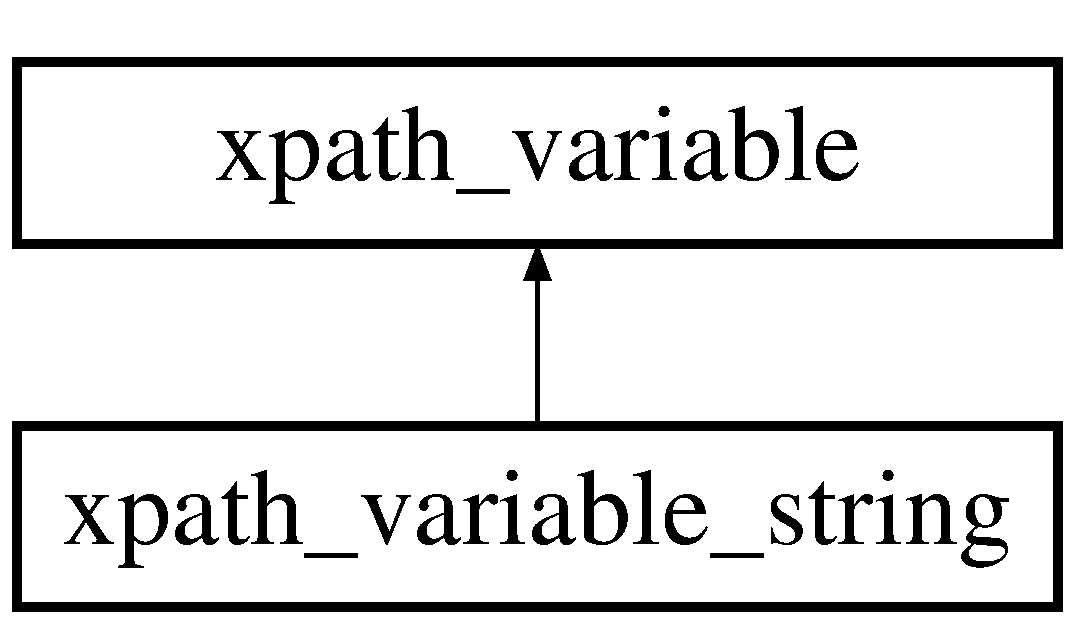
\includegraphics[height=2.000000cm]{structxpath__variable__string}
\end{center}
\end{figure}
\subsection*{Public Member Functions}
\begin{DoxyCompactItemize}
\item 
\hyperlink{structxpath__variable__string_a119d348b7f76371928faa5f5f80df815}{xpath\-\_\-variable\-\_\-string} ()
\item 
\hyperlink{structxpath__variable__string_a8e5e421f2e963e6196d2812a623ee912}{$\sim$xpath\-\_\-variable\-\_\-string} ()
\end{DoxyCompactItemize}
\subsection*{Data Fields}
\begin{DoxyCompactItemize}
\item 
char\-\_\-t $\ast$ \hyperlink{structxpath__variable__string_aeb8a87a8457d2615cd7b766fd3f30559}{value}
\item 
char\-\_\-t \hyperlink{structxpath__variable__string_a5c43cdcc55a620db0e7bdd29b4d56e89}{name} \mbox{[}1\mbox{]}
\end{DoxyCompactItemize}


\subsection{Constructor \& Destructor Documentation}
\hypertarget{structxpath__variable__string_a119d348b7f76371928faa5f5f80df815}{\index{xpath\-\_\-variable\-\_\-string@{xpath\-\_\-variable\-\_\-string}!xpath\-\_\-variable\-\_\-string@{xpath\-\_\-variable\-\_\-string}}
\index{xpath\-\_\-variable\-\_\-string@{xpath\-\_\-variable\-\_\-string}!xpath_variable_string@{xpath\-\_\-variable\-\_\-string}}
\subsubsection[{xpath\-\_\-variable\-\_\-string}]{\setlength{\rightskip}{0pt plus 5cm}xpath\-\_\-variable\-\_\-string\-::xpath\-\_\-variable\-\_\-string (
\begin{DoxyParamCaption}
{}
\end{DoxyParamCaption}
)\hspace{0.3cm}{\ttfamily [inline]}}}\label{structxpath__variable__string_a119d348b7f76371928faa5f5f80df815}
\hypertarget{structxpath__variable__string_a8e5e421f2e963e6196d2812a623ee912}{\index{xpath\-\_\-variable\-\_\-string@{xpath\-\_\-variable\-\_\-string}!$\sim$xpath\-\_\-variable\-\_\-string@{$\sim$xpath\-\_\-variable\-\_\-string}}
\index{$\sim$xpath\-\_\-variable\-\_\-string@{$\sim$xpath\-\_\-variable\-\_\-string}!xpath_variable_string@{xpath\-\_\-variable\-\_\-string}}
\subsubsection[{$\sim$xpath\-\_\-variable\-\_\-string}]{\setlength{\rightskip}{0pt plus 5cm}xpath\-\_\-variable\-\_\-string\-::$\sim$xpath\-\_\-variable\-\_\-string (
\begin{DoxyParamCaption}
{}
\end{DoxyParamCaption}
)\hspace{0.3cm}{\ttfamily [inline]}}}\label{structxpath__variable__string_a8e5e421f2e963e6196d2812a623ee912}


\subsection{Field Documentation}
\hypertarget{structxpath__variable__string_a5c43cdcc55a620db0e7bdd29b4d56e89}{\index{xpath\-\_\-variable\-\_\-string@{xpath\-\_\-variable\-\_\-string}!name@{name}}
\index{name@{name}!xpath_variable_string@{xpath\-\_\-variable\-\_\-string}}
\subsubsection[{name}]{\setlength{\rightskip}{0pt plus 5cm}char\-\_\-t xpath\-\_\-variable\-\_\-string\-::name\mbox{[}1\mbox{]}}}\label{structxpath__variable__string_a5c43cdcc55a620db0e7bdd29b4d56e89}
\hypertarget{structxpath__variable__string_aeb8a87a8457d2615cd7b766fd3f30559}{\index{xpath\-\_\-variable\-\_\-string@{xpath\-\_\-variable\-\_\-string}!value@{value}}
\index{value@{value}!xpath_variable_string@{xpath\-\_\-variable\-\_\-string}}
\subsubsection[{value}]{\setlength{\rightskip}{0pt plus 5cm}char\-\_\-t$\ast$ xpath\-\_\-variable\-\_\-string\-::value}}\label{structxpath__variable__string_aeb8a87a8457d2615cd7b766fd3f30559}


The documentation for this struct was generated from the following file\-:\begin{DoxyCompactItemize}
\item 
System/\hyperlink{pugixml_8cpp}{pugixml.\-cpp}\end{DoxyCompactItemize}

\chapter{File Documentation}
\hypertarget{_be_board_8cc}{\section{H\-W\-Description/\-Be\-Board.cc File Reference}
\label{_be_board_8cc}\index{H\-W\-Description/\-Be\-Board.\-cc@{H\-W\-Description/\-Be\-Board.\-cc}}
}

\hypertarget{_be_board_8h}{\section{H\-W\-Description/\-Be\-Board.h File Reference}
\label{_be_board_8h}\index{H\-W\-Description/\-Be\-Board.\-h@{H\-W\-Description/\-Be\-Board.\-h}}
}


Be\-Board Description class, configs of the Be\-Board.  


{\ttfamily \#include \char`\"{}Definition.\-h\char`\"{}}\\*
{\ttfamily \#include \char`\"{}Module.\-h\char`\"{}}\\*
{\ttfamily \#include $<$vector$>$}\\*
{\ttfamily \#include $<$map$>$}\\*
{\ttfamily \#include $<$boost/cstdint.\-hpp$>$}\\*
\subsection*{Data Structures}
\begin{DoxyCompactItemize}
\item 
class \hyperlink{class_ph2___hw_description_1_1_be_board}{Ph2\-\_\-\-Hw\-Description\-::\-Be\-Board}
\begin{DoxyCompactList}\small\item\em Read/\-Write \hyperlink{class_ph2___hw_description_1_1_be_board}{Be\-Board}'s registers on a file, contains a register map and contains a vector of \hyperlink{class_ph2___hw_description_1_1_module}{Module} which are connected to the \hyperlink{class_ph2___hw_description_1_1_be_board}{Be\-Board}. \end{DoxyCompactList}\end{DoxyCompactItemize}
\subsection*{Namespaces}
\begin{DoxyCompactItemize}
\item 
\hyperlink{namespace_ph2___hw_description}{Ph2\-\_\-\-Hw\-Description}
\begin{DoxyCompactList}\small\item\em Namespace regrouping all the hardware description. \end{DoxyCompactList}\end{DoxyCompactItemize}
\subsection*{Typedefs}
\begin{DoxyCompactItemize}
\item 
typedef std\-::map$<$ std\-::string, \\*
uint16\-\_\-t $>$ \hyperlink{namespace_ph2___hw_description_a2e13fb82c8ed98154c60f9d0f8467d72}{Ph2\-\_\-\-Hw\-Description\-::\-Be\-Board\-Reg\-Map}
<<<<<<< HEAD
\end{DoxyCompactItemize}
\subsection*{Enumerations}
\begin{DoxyCompactItemize}
\item 
enum \hyperlink{namespace_ph2___hw_description_a891c19542f306c932b747f42fe48fc2b}{Ph2\-\_\-\-Hw\-Description\-::nb\-\_\-\-F\-E} \{ \hyperlink{namespace_ph2___hw_description_a891c19542f306c932b747f42fe48fc2baa30d72f6d58dc25b003fbf8bf56b3ace}{Ph2\-\_\-\-Hw\-Description\-::\-S\-I\-N\-G\-L\-E\-\_\-\-F\-E}, 
\hyperlink{namespace_ph2___hw_description_a891c19542f306c932b747f42fe48fc2ba6e0b877d015d017f61b07618e057c452}{Ph2\-\_\-\-Hw\-Description\-::\-F\-E\-\_\-\-T\-R\-G}, 
\hyperlink{namespace_ph2___hw_description_a891c19542f306c932b747f42fe48fc2bae3b57cb16641bb367bfc57a00315a4ca}{Ph2\-\_\-\-Hw\-Description\-::\-D\-U\-A\-L\-\_\-\-F\-E}
 \}
=======
>>>>>>> origin/Dev
\end{DoxyCompactItemize}


\subsection{Detailed Description}
Be\-Board Description class, configs of the Be\-Board. \begin{DoxyAuthor}{Author}
Lorenzo B\-I\-D\-E\-G\-A\-I\-N 
\end{DoxyAuthor}
\begin{DoxyDate}{Date}
14/07/14
\end{DoxyDate}
Support \-: mail to \-: \href{mailto:lorenzo.bidegain@cern.ch}{\tt lorenzo.\-bidegain@cern.\-ch} 
\hypertarget{_cbc_8cc}{
\section{HWDescription/Cbc.cc File Reference}
\label{_cbc_8cc}\index{HWDescription/Cbc.cc@{HWDescription/Cbc.cc}}
}
{\tt \#include \char`\"{}Cbc.h\char`\"{}}\par
{\tt \#include $<$fstream$>$}\par
{\tt \#include $<$cstdio$>$}\par
{\tt \#include $<$sstream$>$}\par
{\tt \#include $<$iostream$>$}\par
{\tt \#include $<$string.h$>$}\par
{\tt \#include $<$iomanip$>$}\par
{\tt \#include \char`\"{}Definition.h\char`\"{}}\par
\subsection*{Namespaces}
\begin{CompactItemize}
\item 
namespace \hyperlink{namespace_ph2___hw_description}{Ph2\_\-Hw\-Description}
\end{CompactItemize}

\hypertarget{_cbc_8h}{\section{H\-W\-Description/\-Cbc.h File Reference}
\label{_cbc_8h}\index{H\-W\-Description/\-Cbc.\-h@{H\-W\-Description/\-Cbc.\-h}}
}


Cbc Description class, config of the Cbcs.  


{\ttfamily \#include \char`\"{}Front\-End\-Description.\-h\char`\"{}}\\*
{\ttfamily \#include \char`\"{}Cbc\-Reg\-Item.\-h\char`\"{}}\\*
{\ttfamily \#include $<$iostream$>$}\\*
{\ttfamily \#include $<$map$>$}\\*
{\ttfamily \#include $<$string$>$}\\*
{\ttfamily \#include $<$boost/cstdint.\-hpp$>$}\\*
\subsection*{Data Structures}
\begin{DoxyCompactItemize}
\item 
class \hyperlink{class_ph2___hw_description_1_1_cbc}{Ph2\-\_\-\-Hw\-Description\-::\-Cbc}
\begin{DoxyCompactList}\small\item\em Read/\-Write \hyperlink{class_ph2___hw_description_1_1_cbc}{Cbc}'s registers on a file. \end{DoxyCompactList}\item 
struct \hyperlink{struct_ph2___hw_description_1_1_cbc_comparer}{Ph2\-\_\-\-Hw\-Description\-::\-Cbc\-Comparer}
\begin{DoxyCompactList}\small\item\em Compare two \hyperlink{class_ph2___hw_description_1_1_cbc}{Cbc} by their I\-D. \end{DoxyCompactList}\end{DoxyCompactItemize}
\subsection*{Namespaces}
\begin{DoxyCompactItemize}
\item 
\hyperlink{namespace_ph2___hw_description}{Ph2\-\_\-\-Hw\-Description}
\begin{DoxyCompactList}\small\item\em Namespace regrouping all the hardware description. \end{DoxyCompactList}\end{DoxyCompactItemize}
\subsection*{Macros}
\begin{DoxyCompactItemize}
\item 
\#define \hyperlink{_cbc_8h_ad406c895476128d696804038e617141b}{default\-\_\-file}~\char`\"{}default\-\_\-file.\-txt\char`\"{}
\end{DoxyCompactItemize}
\subsection*{Typedefs}
\begin{DoxyCompactItemize}
\item 
typedef std\-::map$<$ std\-::string, \\*
Cbc\-Reg\-Item $>$ \hyperlink{namespace_ph2___hw_description_a9a23b373068f169aa67ca1d22c9a6001}{Ph2\-\_\-\-Hw\-Description\-::\-Cbc\-Reg\-Map}
\end{DoxyCompactItemize}


\subsection{Detailed Description}
Cbc Description class, config of the Cbcs. \begin{DoxyAuthor}{Author}
Lorenzo B\-I\-D\-E\-G\-A\-I\-N 
\end{DoxyAuthor}
\begin{DoxyDate}{Date}
25/06/14
\end{DoxyDate}
Support \-: mail to \-: \href{mailto:lorenzo.bidegain@cern.ch}{\tt lorenzo.\-bidegain@cern.\-ch} 

\subsection{Macro Definition Documentation}
\hypertarget{_cbc_8h_ad406c895476128d696804038e617141b}{\index{Cbc.\-h@{Cbc.\-h}!default\-\_\-file@{default\-\_\-file}}
\index{default\-\_\-file@{default\-\_\-file}!Cbc.h@{Cbc.\-h}}
\subsubsection[{default\-\_\-file}]{\setlength{\rightskip}{0pt plus 5cm}\#define default\-\_\-file~\char`\"{}default\-\_\-file.\-txt\char`\"{}}}\label{_cbc_8h_ad406c895476128d696804038e617141b}

\hypertarget{_cbc_reg_item_8h}{\section{H\-W\-Description/\-Cbc\-Reg\-Item.h File Reference}
\label{_cbc_reg_item_8h}\index{H\-W\-Description/\-Cbc\-Reg\-Item.\-h@{H\-W\-Description/\-Cbc\-Reg\-Item.\-h}}
}
\subsection*{Data Structures}
\begin{DoxyCompactItemize}
\item 
struct \hyperlink{struct_ph2___hw_description_1_1_cbc_reg_item}{Ph2\-\_\-\-Hw\-Description\-::\-Cbc\-Reg\-Item}
\item 
struct \hyperlink{struct_ph2___hw_description_1_1_reg_item_comparer}{Ph2\-\_\-\-Hw\-Description\-::\-Reg\-Item\-Comparer}
\end{DoxyCompactItemize}
\subsection*{Namespaces}
\begin{DoxyCompactItemize}
\item 
\hyperlink{namespace_ph2___hw_description}{Ph2\-\_\-\-Hw\-Description}
\end{DoxyCompactItemize}

\hypertarget{_definition_8h}{
\section{HWDescription/Definition.h File Reference}
\label{_definition_8h}\index{HWDescription/Definition.h@{HWDescription/Definition.h}}
}
\subsection*{Defines}
\begin{CompactItemize}
\item 
\#define \hyperlink{_definition_8h_522d1a46e55b54c8ff9ec3275c60d73a}{XML\_\-DESCRIPTION\_\-FILE\_\-2CBC}~\char`\"{}settings/HWDescription\_\-2CBC.xml\char`\"{}
\item 
\#define \hyperlink{_definition_8h_26d84c24d1a2341a0fa6d42a89921628}{XML\_\-DESCRIPTION\_\-FILE\_\-8CBC}~\char`\"{}settings/HWDescription\_\-8CBC.xml\char`\"{}
\item 
\#define \hyperlink{_definition_8h_7538d40fca6562ecc1768f6d07cef2fa}{I2C\_\-CTRL\_\-ENABLE}~0x000009F4
\item 
\#define \hyperlink{_definition_8h_b1dd2d69bec1712857cc2a103c85c26d}{I2C\_\-CTRL\_\-DISABLE}~0
\item 
\#define \hyperlink{_definition_8h_8d3f448d28b023f560e3df976bb3ff9c}{I2C\_\-STROBE}~1
\item 
\#define \hyperlink{_definition_8h_ae239b4919cbd8d8dced934150986de3}{I2C\_\-M16B}~0
\item 
\#define \hyperlink{_definition_8h_c030aa7b3fbd8b2432a9c66fc49fc4ae}{I2C\_\-MEM}~1
\item 
\#define \hyperlink{_definition_8h_7978167075eb8954c1090fc7ce9647c6}{I2C\_\-WRITE\_\-ADDR}~0x09
\item 
\#define \hyperlink{_definition_8h_11a0148c64950f3315f38d957cd43d37}{I2C\_\-READ\_\-ADDR}~0x06
\item 
\#define \hyperlink{_definition_8h_b15137f7c592d05573de99f078516157}{I2C\_\-SLAVE}~0x5B
\item 
\#define \hyperlink{_definition_8h_e308275dafb538f2511ea285fea768d0}{I2C\_\-COMMAND}~\char`\"{}user\_\-wb\_\-ttc\_\-fmc\_\-regs.cbc\_\-reg\_\-i2c\_\-command\char`\"{}
\item 
\#define \hyperlink{_definition_8h_46aaa2293185dfc3cd655f65bea7f614}{I2C\_\-REPLY}~\char`\"{}user\_\-wb\_\-ttc\_\-fmc\_\-regs.cbc\_\-reg\_\-i2c\_\-reply\char`\"{}
\item 
\#define \hyperlink{_definition_8h_15db09e24617ea5c5843213672ac8a03}{I2C\_\-SETTINGS}~\char`\"{}user\_\-wb\_\-ttc\_\-fmc\_\-regs.cbc\_\-reg\_\-i2c\_\-settings\char`\"{}
\item 
\#define \hyperlink{_definition_8h_30957298974d3b5c605a9e6e3cf33ff9}{MAX\_\-NB\_\-LOOP}~50
\item 
\#define \hyperlink{_definition_8h_9b229c5fa667622ae84c26cbbfca2c4a}{BOARD\_\-TYPE}~\char`\"{}board\_\-id\char`\"{}
\item 
\#define \hyperlink{_definition_8h_5a209f781c62e738bb2f3868604fbe77}{FW\_\-VERSION\_\-MAJOR}~\char`\"{}firm\_\-id.firmware\_\-major\char`\"{}
\item 
\#define \hyperlink{_definition_8h_e224d2fae5df95eef5b8b1638b714731}{FW\_\-VERSION\_\-MINOR}~\char`\"{}firm\_\-id.firmware\_\-minor\char`\"{}
\item 
\#define \hyperlink{_definition_8h_46d23f1b70547c7ec03a7ede5a4a53c1}{FW\_\-VERSION\_\-BUILD}~\char`\"{}firm\_\-id.firmware\_\-build\char`\"{}
\item 
\#define \hyperlink{_definition_8h_ce8447cf1974d876d5655fb2fb48f7a9}{FMC1\_\-PRESENT}~\char`\"{}status.fmc1\_\-present\char`\"{}
\item 
\#define \hyperlink{_definition_8h_dc6f5f1944441c702829bb535878c480}{FMC2\_\-PRESENT}~\char`\"{}status.fmc2\_\-present\char`\"{}
\item 
\#define \hyperlink{_definition_8h_6124cfaca7b122eb740cc81165fdb52d}{FMC\_\-USER\_\-BOARD\_\-ID}~\char`\"{}user\_\-wb\_\-ttc\_\-fmc\_\-regs.user\_\-board\_\-id\char`\"{}
\item 
\#define \hyperlink{_definition_8h_63344015089bba1295e33de70c0bd6d1}{FMC\_\-USER\_\-SYS\_\-ID}~\char`\"{}user\_\-wb\_\-ttc\_\-fmc\_\-regs.user\_\-sys\_\-id\char`\"{}
\item 
\#define \hyperlink{_definition_8h_e326374c67375e752225499c19882801}{FMC\_\-USER\_\-VERSION}~\char`\"{}user\_\-wb\_\-ttc\_\-fmc\_\-regs.user\_\-version\char`\"{}
\item 
\#define \hyperlink{_definition_8h_6a7f90395054dfa1a2f6521213aad848}{SRAM1}~\char`\"{}sram1\char`\"{}
\item 
\#define \hyperlink{_definition_8h_14684bbbabb20ef143bc395b2c7e2ed9}{SRAM2}~\char`\"{}sram2\char`\"{}
\item 
\#define \hyperlink{_definition_8h_69322dcaf50029bc06b197cbcac24296}{SRAM1\_\-256}~\char`\"{}sram1\_\-256\char`\"{}
\item 
\#define \hyperlink{_definition_8h_1c40ef19c013212b46bd2f866d2d7367}{SRAM2\_\-256}~\char`\"{}sram2\_\-256\char`\"{}
\item 
\#define \hyperlink{_definition_8h_df5585d61d19b17bc9af074a461fde93}{SRAM1\_\-USR\_\-LOGIC}~\char`\"{}ctrl\_\-sram.sram1\_\-user\_\-logic\char`\"{}
\item 
\#define \hyperlink{_definition_8h_d891becc0588c44642479f53d559c1a5}{SRAM2\_\-USR\_\-LOGIC}~\char`\"{}ctrl\_\-sram.sram2\_\-user\_\-logic\char`\"{}
\item 
\#define \hyperlink{_definition_8h_96bfb08d3abc89fde1c50f2db0b640de}{SRAM1\_\-END\_\-READOUT}~\char`\"{}user\_\-wb\_\-ttc\_\-fmc\_\-regs.pc\_\-commands.SRAM1\_\-end\_\-readout\char`\"{}
\item 
\#define \hyperlink{_definition_8h_df4e9d9d29b9c2e8e501dae3131be2a3}{SRAM2\_\-END\_\-READOUT}~\char`\"{}user\_\-wb\_\-ttc\_\-fmc\_\-regs.pc\_\-commands.SRAM2\_\-end\_\-readout\char`\"{}
\item 
\#define \hyperlink{_definition_8h_08761f200e1c7a6fe97e09d7af9c7a15}{SRAM1\_\-FULL}~\char`\"{}user\_\-wb\_\-ttc\_\-fmc\_\-regs.flags.SRAM1\_\-full\char`\"{}
\item 
\#define \hyperlink{_definition_8h_937e26b9dc4d1f265bbc8982b410451b}{SRAM2\_\-FULL}~\char`\"{}user\_\-wb\_\-ttc\_\-fmc\_\-regs.flags.SRAM2\_\-full\char`\"{}
\item 
\#define \hyperlink{_definition_8h_6190016044b4e4aafb00bc3767600a34}{FAKE\_\-DATA}~\char`\"{}user\_\-wb\_\-ttc\_\-fmc\_\-regs.pc\_\-commands.CBC\_\-DATA\_\-GENE\char`\"{}
\item 
\#define \hyperlink{_definition_8h_c2006ced84fd829c1eaea6ee77c73fce}{EXT\_\-TRG}~\char`\"{}user\_\-wb\_\-ttc\_\-fmc\_\-regs.pc\_\-commands.TRIGGER\_\-SEL\char`\"{}
\item 
\#define \hyperlink{_definition_8h_67670806b37e9b321f2d1dc4a45f55a2}{HYBRID\_\-TYPE}~\char`\"{}hybrid\_\-type\char`\"{}
\item 
\#define \hyperlink{_definition_8h_eae1c06b6a23a69b44f7e8b476d980c8}{HYBRID\_\-VERSION}~\char`\"{}user\_\-wb\_\-ttc\_\-fmc\_\-regs.new.hybrid\_\-version\char`\"{}
\item 
\#define \hyperlink{_definition_8h_d2ba3d00a6d2c7308d2ff50ea039231f}{NB\_\-FE}~\char`\"{}nb\_\-FE\char`\"{}
\item 
\#define \hyperlink{_definition_8h_7da27b2738428e3dfeb39e351e551556}{CBC\_\-EXPECTED}~\char`\"{}CBC\_\-expected\char`\"{}
\item 
\#define \hyperlink{_definition_8h_4c95b734f201124f65fdf525484f905c}{CBC\_\-PACKET\_\-NB}~\char`\"{}user\_\-wb\_\-ttc\_\-fmc\_\-regs.pc\_\-commands.CBC\_\-DATA\_\-PACKET\_\-NUMBER\char`\"{}
\item 
\#define \hyperlink{_definition_8h_b41e5a6624129af07cf04896a2638e05}{CBC\_\-TEST\_\-PULSE\_\-VALID}~\char`\"{}COMMISSIONNING\_\-MODE\_\-CBC\_\-TEST\_\-PULSE\_\-VALID\char`\"{}
\item 
\#define \hyperlink{_definition_8h_a8b47c8d93bc3a0a17f13d7aba88eebd}{CBC\_\-DATA\_\-GENE}~\char`\"{}user\_\-wb\_\-ttc\_\-fmc\_\-regs.pc\_\-commands.CBC\_\-DATA\_\-GENE\char`\"{}
\item 
\#define \hyperlink{_definition_8h_f707b6c693823387a84c1ae5b5dc01c7}{CBC\_\-TRIGGER\_\-1SHOT}~\char`\"{}user\_\-wb\_\-ttc\_\-fmc\_\-regs.cbc\_\-acquisition.CBC\_\-TRIGGER\_\-ONE\_\-SHOT\char`\"{}
\item 
\#define \hyperlink{_definition_8h_74f2bb936c6db739349d53796624df22}{CBC\_\-STUB\_\-LATENCY}~\char`\"{}cbc\_\-stubdata\_\-latency\_\-adjust\char`\"{}
\item 
\#define \hyperlink{_definition_8h_dcbbe8574bdf346be21ae23451c410ec}{CBC\_\-STUB\_\-LATENCY\_\-FE1}~\char`\"{}cbc\_\-stubdata\_\-latency\_\-adjust\_\-fe1\char`\"{}
\item 
\#define \hyperlink{_definition_8h_99153490571202993a0d92d1ffb62df0}{CBC\_\-STUB\_\-LATENCY\_\-FE2}~\char`\"{}cbc\_\-stubdata\_\-latency\_\-adjust\_\-fe2\char`\"{}
\item 
\#define \hyperlink{_definition_8h_980fdc4242ab14da9fcd648b1e9a50a4}{CBC\_\-I2C\_\-CMD\_\-ACK}~\char`\"{}cbc\_\-i2c\_\-cmd\_\-ack\char`\"{}
\item 
\#define \hyperlink{_definition_8h_8a4f3b344351ac3f9e05f3a3d27ffbf6}{CBC\_\-I2C\_\-CMD\_\-ACK\_\-FE1}~\char`\"{}cbc\_\-i2c\_\-cmd\_\-ack\_\-fe1\char`\"{}
\item 
\#define \hyperlink{_definition_8h_d7ef355ab00621a8d2984b3a4d2b5336}{CBC\_\-I2C\_\-CMD\_\-ACK\_\-FE2}~\char`\"{}cbc\_\-i2c\_\-cmd\_\-ack\_\-fe2\char`\"{}
\item 
\#define \hyperlink{_definition_8h_a92f4a416201bbe9742da9f72ba0bb46}{CBC\_\-I2C\_\-CMD\_\-RQ}~\char`\"{}cbc\_\-i2c\_\-cmd\_\-rq\char`\"{}
\item 
\#define \hyperlink{_definition_8h_27f1d47d65b52569c75ae7abb12c850c}{CBC\_\-I2C\_\-CMD\_\-RQ\_\-FE1}~\char`\"{}cbc\_\-i2c\_\-cmd\_\-rq\_\-fe1\char`\"{}
\item 
\#define \hyperlink{_definition_8h_386e61ed089e53095e19b1dded969001}{CBC\_\-I2C\_\-CMD\_\-RQ\_\-FE2}~\char`\"{}cbc\_\-i2c\_\-cmd\_\-rq\_\-fe2\char`\"{}
\item 
\#define \hyperlink{_definition_8h_339750768b74eeb2a5e15d27002e5ed1}{CBC\_\-HARD\_\-RESET}~\char`\"{}cbc\_\-hard\_\-reset\char`\"{}
\item 
\#define \hyperlink{_definition_8h_1afae7c30406c0520e384fa1806e97ca}{CBC\_\-HARD\_\-RESET\_\-FE1}~\char`\"{}cbc\_\-hard\_\-reset\_\-fe1\char`\"{}
\item 
\#define \hyperlink{_definition_8h_e6dcd5d0b1ff293b4ad62fe648e34127}{CBC\_\-HARD\_\-RESET\_\-FE2}~\char`\"{}cbc\_\-hard\_\-reset\_\-fe2\char`\"{}
\item 
\#define \hyperlink{_definition_8h_46c24affadd18b38f8f180c29996c917}{CBC\_\-FAST\_\-RESET}~\char`\"{}cbc\_\-fast\_\-reset\char`\"{}
\item 
\#define \hyperlink{_definition_8h_14ca43ce56b6ba3282562ec26d4dd1d4}{CBC\_\-FAST\_\-RESET\_\-FE1}~\char`\"{}cbc\_\-fast\_\-reset\_\-fe1\char`\"{}
\item 
\#define \hyperlink{_definition_8h_ac0c28e4301536787f75b2b7c8f8a4ab}{CBC\_\-FAST\_\-RESET\_\-FE2}~\char`\"{}cbc\_\-fast\_\-reset\_\-fe2\char`\"{}
\item 
\#define \hyperlink{_definition_8h_21929d3fe4a97a1b854110f3cb1c3f58}{ENABLE\_\-FE0\_\-CBC0}~\char`\"{}user\_\-wb\_\-ttc\_\-fmc\_\-regs.FE0.CBC0\char`\"{}
\item 
\#define \hyperlink{_definition_8h_22c3189db97e8a23a0ebd2413daefb67}{ENABLE\_\-FE0\_\-CBC1}~\char`\"{}user\_\-wb\_\-ttc\_\-fmc\_\-regs.FE0.CBC1\char`\"{}
\item 
\#define \hyperlink{_definition_8h_79ebea1b1cff5aca72560a5165cef784}{ENABLE\_\-FE0\_\-CBC2}~\char`\"{}user\_\-wb\_\-ttc\_\-fmc\_\-regs.FE0.CBC2\char`\"{}
\item 
\#define \hyperlink{_definition_8h_e2cf6493ba65a5a24f9d9171c27c2a2e}{ENABLE\_\-FE0\_\-CBC3}~\char`\"{}user\_\-wb\_\-ttc\_\-fmc\_\-regs.FE0.CBC3\char`\"{}
\item 
\#define \hyperlink{_definition_8h_bcd6b5364cbcc9c22b7ca984e5b68b83}{ENABLE\_\-FE0\_\-CBC4}~\char`\"{}user\_\-wb\_\-ttc\_\-fmc\_\-regs.FE0.CBC4\char`\"{}
\item 
\#define \hyperlink{_definition_8h_d353c3df69d1a4593e3bb3cf0c8b555f}{ENABLE\_\-FE0\_\-CBC5}~\char`\"{}user\_\-wb\_\-ttc\_\-fmc\_\-regs.FE0.CBC5\char`\"{}
\item 
\#define \hyperlink{_definition_8h_b00b99d0589e0c7cb397936f7cceeb1e}{ENABLE\_\-FE0\_\-CBC6}~\char`\"{}user\_\-wb\_\-ttc\_\-fmc\_\-regs.FE0.CBC6\char`\"{}
\item 
\#define \hyperlink{_definition_8h_1de9fce1a97c53ca033c99051bae5da7}{ENABLE\_\-FE0\_\-CBC7}~\char`\"{}user\_\-wb\_\-ttc\_\-fmc\_\-regs.FE0.CBC7\char`\"{}
\item 
\#define \hyperlink{_definition_8h_6148f48ad50c9763bc623d43dbff9298}{ENABLE\_\-FE0\_\-CBC8}~\char`\"{}user\_\-wb\_\-ttc\_\-fmc\_\-regs.FE0.CBC8\char`\"{}
\item 
\#define \hyperlink{_definition_8h_9c76e69061159cc4092e21ef4433a6e7}{ENABLE\_\-FE0\_\-CBC9}~\char`\"{}user\_\-wb\_\-ttc\_\-fmc\_\-regs.FE0.CBC9\char`\"{}
\item 
\#define \hyperlink{_definition_8h_674d82485e0138e446a3bf7005ecbe0f}{ENABLE\_\-FE0\_\-CBC10}~\char`\"{}user\_\-wb\_\-ttc\_\-fmc\_\-regs.FE0.CBC10\char`\"{}
\item 
\#define \hyperlink{_definition_8h_77506b853e03009d0f5aee68d4e9ba84}{ENABLE\_\-FE0\_\-CBC11}~\char`\"{}user\_\-wb\_\-ttc\_\-fmc\_\-regs.FE0.CBC11\char`\"{}
\item 
\#define \hyperlink{_definition_8h_05b144d4533ad9c4205feb0eb5f736e6}{ENABLE\_\-FE0\_\-CBC12}~\char`\"{}user\_\-wb\_\-ttc\_\-fmc\_\-regs.FE0.CBC12\char`\"{}
\item 
\#define \hyperlink{_definition_8h_8225af337a0f9f4ddaadf0bbc4264c02}{ENABLE\_\-FE0\_\-CBC13}~\char`\"{}user\_\-wb\_\-ttc\_\-fmc\_\-regs.FE0.CBC13\char`\"{}
\item 
\#define \hyperlink{_definition_8h_74da8be115351dfc75ae35ca834a8147}{ENABLE\_\-FE0\_\-CBC14}~\char`\"{}user\_\-wb\_\-ttc\_\-fmc\_\-regs.FE0.CBC14\char`\"{}
\item 
\#define \hyperlink{_definition_8h_252b8d73c177c269f546f487884c7eff}{ENABLE\_\-FE0\_\-CBC15}~\char`\"{}user\_\-wb\_\-ttc\_\-fmc\_\-regs.FE0.CBC15\char`\"{}
\item 
\#define \hyperlink{_definition_8h_de36fc7aee3ea334c79116a6274842cb}{CBC\_\-FE0\_\-ENABLED}~\char`\"{}user\_\-wb\_\-ttc\_\-fmc\_\-regs.FE0.enabled\char`\"{}
\item 
\#define \hyperlink{_definition_8h_03317145939625cba307ba446b365986}{ENABLE\_\-FE1\_\-CBC0}~\char`\"{}user\_\-wb\_\-ttc\_\-fmc\_\-regs.FE1.CBC0\char`\"{}
\item 
\#define \hyperlink{_definition_8h_b76d774c8ed60fab0eeb6e8ef87a2ded}{ENABLE\_\-FE1\_\-CBC1}~\char`\"{}user\_\-wb\_\-ttc\_\-fmc\_\-regs.FE1.CBC1\char`\"{}
\item 
\#define \hyperlink{_definition_8h_8bfad8c6a0b94b20a3a9281589b31471}{ENABLE\_\-FE1\_\-CBC2}~\char`\"{}user\_\-wb\_\-ttc\_\-fmc\_\-regs.FE1.CBC2\char`\"{}
\item 
\#define \hyperlink{_definition_8h_263b5f189fbc3d3387e10e2f32d03abb}{ENABLE\_\-FE1\_\-CBC3}~\char`\"{}user\_\-wb\_\-ttc\_\-fmc\_\-regs.FE1.CBC3\char`\"{}
\item 
\#define \hyperlink{_definition_8h_98470137a318927b22805ede8fcde0f4}{ENABLE\_\-FE1\_\-CBC4}~\char`\"{}user\_\-wb\_\-ttc\_\-fmc\_\-regs.FE1.CBC4\char`\"{}
\item 
\#define \hyperlink{_definition_8h_cb93a071c9d4140aa188e7c8f976934d}{ENABLE\_\-FE1\_\-CBC5}~\char`\"{}user\_\-wb\_\-ttc\_\-fmc\_\-regs.FE1.CBC5\char`\"{}
\item 
\#define \hyperlink{_definition_8h_e874f3583b542160e906512331c4cc88}{ENABLE\_\-FE1\_\-CBC6}~\char`\"{}user\_\-wb\_\-ttc\_\-fmc\_\-regs.FE1.CBC6\char`\"{}
\item 
\#define \hyperlink{_definition_8h_bce65c16723daa8105c8b16cbfa4fe51}{ENABLE\_\-FE1\_\-CBC7}~\char`\"{}user\_\-wb\_\-ttc\_\-fmc\_\-regs.FE1.CBC7\char`\"{}
\item 
\#define \hyperlink{_definition_8h_7f9cd1649eb893431936cdf4c7f3c282}{ENABLE\_\-FE1\_\-CBC8}~\char`\"{}user\_\-wb\_\-ttc\_\-fmc\_\-regs.FE1.CBC8\char`\"{}
\item 
\#define \hyperlink{_definition_8h_3d710db3abf22fac46e52b3645670616}{ENABLE\_\-FE1\_\-CBC9}~\char`\"{}user\_\-wb\_\-ttc\_\-fmc\_\-regs.FE1.CBC9\char`\"{}
\item 
\#define \hyperlink{_definition_8h_062b817ea9e2def85b97d1c0877f46b7}{ENABLE\_\-FE1\_\-CBC10}~\char`\"{}user\_\-wb\_\-ttc\_\-fmc\_\-regs.FE1.CBC10\char`\"{}
\item 
\#define \hyperlink{_definition_8h_48cece7e1f97f624fe98af09df709209}{ENABLE\_\-FE1\_\-CBC11}~\char`\"{}user\_\-wb\_\-ttc\_\-fmc\_\-regs.FE1.CBC11\char`\"{}
\item 
\#define \hyperlink{_definition_8h_aa4a44550314c57ea9bfe01c1288a2c6}{ENABLE\_\-FE1\_\-CBC12}~\char`\"{}user\_\-wb\_\-ttc\_\-fmc\_\-regs.FE1.CBC12\char`\"{}
\item 
\#define \hyperlink{_definition_8h_98c3bccbb72aa385251a0145628396ce}{ENABLE\_\-FE1\_\-CBC13}~\char`\"{}user\_\-wb\_\-ttc\_\-fmc\_\-regs.FE1.CBC13\char`\"{}
\item 
\#define \hyperlink{_definition_8h_b6bb263484b332b72f2fec89a0dda4fc}{ENABLE\_\-FE1\_\-CBC14}~\char`\"{}user\_\-wb\_\-ttc\_\-fmc\_\-regs.FE1.CBC14\char`\"{}
\item 
\#define \hyperlink{_definition_8h_396018336770bb4351eba3aa75cd7474}{ENABLE\_\-FE1\_\-CBC15}~\char`\"{}user\_\-wb\_\-ttc\_\-fmc\_\-regs.FE1.CBC15\char`\"{}
\item 
\#define \hyperlink{_definition_8h_83f524d50b61345b68f47f01131af8f4}{CBC\_\-FE1\_\-ENABLED}~\char`\"{}user\_\-wb\_\-ttc\_\-fmc\_\-regs.FE1.enabled\char`\"{}
\item 
\#define \hyperlink{_definition_8h_a8f2e0c6d69fa30c6f3df3a1ce79191b}{DELAY\_\-AF\_\-FAST\_\-RESET}~\char`\"{}COMMISSIONNING\_\-MODE\_\-DELAY\_\-AFTER\_\-FAST\_\-RESET\char`\"{}
\item 
\#define \hyperlink{_definition_8h_54b90cd00f1ecb699b4addd24a1991f5}{DELAY\_\-AF\_\-L1A}~\char`\"{}COMMISSIONNING\_\-MODE\_\-DELAY\_\-AFTER\_\-L1A\char`\"{}
\item 
\#define \hyperlink{_definition_8h_de36f0b97b019d8e26695fc406262b42}{DELAY\_\-AF\_\-TEST\_\-PULSE}~\char`\"{}COMMISSIONNING\_\-MODE\_\-DELAY\_\-AFTER\_\-TEST\_\-PULSE\char`\"{}
\item 
\#define \hyperlink{_definition_8h_001a688d4bf711101d3b626ba6ae8726}{BREAK\_\-TRIGGER}~\char`\"{}break\_\-trigger\char`\"{}
\item 
\#define \hyperlink{_definition_8h_11ea004b3c38d4dae3309a13db5b6f78}{INT\_\-TRIGGER\_\-FREQ}~\char`\"{}user\_\-wb\_\-ttc\_\-fmc\_\-regs.pc\_\-commands.INT\_\-TRIGGER\_\-FREQ\char`\"{}
\item 
\#define \hyperlink{_definition_8h_1f0933a2debf91dff9cf62493a7d0225}{TRIGGER\_\-SELECT}~\char`\"{}user\_\-wb\_\-ttc\_\-fmc\_\-regs.pc\_\-commands.TRIGGER\_\-SEL\char`\"{}
\item 
\#define \hyperlink{_definition_8h_1489698bb660d3265c22ac35ab990bdc}{PC\_\-CONFIG\_\-OK}~\char`\"{}user\_\-wb\_\-ttc\_\-fmc\_\-regs.pc\_\-commands.PC\_\-config\_\-ok\char`\"{}
\item 
\#define \hyperlink{_definition_8h_b207427d943afb5b5fc19364720a69a7}{SPURIOUS\_\-FRAME}~\char`\"{}user\_\-wb\_\-ttc\_\-fmc\_\-regs.pc\_\-commands.SPURIOUS\_\-FRAME\char`\"{}
\item 
\#define \hyperlink{_definition_8h_29d2e6a95762c3eac0a1a346b80c9749}{FORCE\_\-BG0\_\-START}~\char`\"{}user\_\-wb\_\-ttc\_\-fmc\_\-regs.pc\_\-commands2.force\_\-BG0\_\-start\char`\"{}
\item 
\#define \hyperlink{_definition_8h_ee17fc2a301953d9c76d8e9f71afcc70}{CMD\_\-START\_\-VALID}~\char`\"{}user\_\-wb\_\-ttc\_\-fmc\_\-regs.status\_\-flags.CMD\_\-START\_\-VALID\char`\"{}
\item 
\#define \hyperlink{_definition_8h_bec4b50692225e50c27448e9a5bee66a}{FE\_\-EXPECTED}~\char`\"{}FE\_\-expected\char`\"{}
\item 
\#define \hyperlink{_definition_8h_a816b503e037321d1934b973f7e33028}{RQ}~\char`\"{}COMMISSIONNING\_\-MODE\_\-RQ\char`\"{}
\item 
\#define \hyperlink{_definition_8h_9b250570624323c4222a15d1cd6b8005}{ACQ\_\-MODE}~\char`\"{}user\_\-wb\_\-ttc\_\-fmc\_\-regs.pc\_\-commands.ACQ\_\-MODE\char`\"{}
\item 
\#define \hyperlink{_definition_8h_b4cc301c3b8aa0dce7713b7d025c2789}{CLOCK\_\-SHIFT}~\char`\"{}user\_\-wb\_\-ttc\_\-fmc\_\-regs.pc\_\-commands2.clock\_\-shift\char`\"{}
\item 
\#define \hyperlink{_definition_8h_001731cf7d6166aebeaa24ba4df58bf2}{NEG\_\-LOGIC\_\-CBC}~\char`\"{}user\_\-wb\_\-ttc\_\-fmc\_\-regs.pc\_\-commands2.negative\_\-logic\_\-CBC\char`\"{}
\item 
\#define \hyperlink{_definition_8h_3f8b0dba172c42abbc1d2909bce9fcfa}{NEG\_\-LOGIC\_\-STTS}~\char`\"{}user\_\-wb\_\-ttc\_\-fmc\_\-regs.pc\_\-commands2.negative\_\-logic\_\-s\-TTS\char`\"{}
\item 
\#define \hyperlink{_definition_8h_94a72e10ee4b5a41ce4221a48ffe5f06}{POLARITY}~\char`\"{}user\_\-wb\_\-ttc\_\-fmc\_\-regs.pc\_\-commands2.polarity\_\-tlu\char`\"{}
\item 
\#define \hyperlink{_definition_8h_799517031a8334a42807b119bb456c53}{TIME\_\-OUT}~5
\item 
\#define \hyperlink{_definition_8h_89acf5b5983235845ea7c7d849f4ed9f}{CBC\_\-EVENT\_\-SIZE\_\-32}~9
\item 
\#define \hyperlink{_definition_8h_da4d3dd73049956f322b901f7ad88f2c}{EVENT\_\-HEADER\_\-TDC\_\-SIZE\_\-32}~6
\item 
\#define \hyperlink{_definition_8h_b48bd5f5134661dcc42a31501acb8ff5}{EVENT\_\-HEADER\_\-SIZE\_\-32}~5
\item 
\#define \hyperlink{_definition_8h_a99523d4b33e4cd1d7bc24ae748b5868}{CBC\_\-EVENT\_\-SIZE\_\-CHAR}~9 $\ast$ 4
\item 
\#define \hyperlink{_definition_8h_10bdb18b33b0f33a0f214cdf57c2ed6c}{EVENT\_\-HEADER\_\-TDC\_\-SIZE\_\-CHAR}~6 $\ast$ 4
\item 
\#define \hyperlink{_definition_8h_133dfc01f9d7f575fc8f020e657dcfc0}{EVENT\_\-HEADER\_\-SIZE\_\-CHAR}~5 $\ast$ 4
\item 
\#define \hyperlink{_definition_8h_f02f6ff9a143548736b70c9b5dd340ef}{OFFSET\_\-BUNCH}~8
\item 
\#define \hyperlink{_definition_8h_80ed4da02244b01e9002b83b08622833}{WIDTH\_\-BUNCH}~24
\item 
\#define \hyperlink{_definition_8h_7e3f5dcd64e350b19cfe6ac8d8b9de55}{OFFSET\_\-ORBIT}~1$\ast$32+8
\item 
\#define \hyperlink{_definition_8h_a9aa442bb5c1632ae55291cc8745df4f}{WIDTH\_\-ORBIT}~24
\item 
\#define \hyperlink{_definition_8h_a726e7f33789f31d51f8e23c8027331f}{OFFSET\_\-LUMI}~2$\ast$32+8
\item 
\#define \hyperlink{_definition_8h_8e0d7d1baf50ff405315799885e5fe1f}{WIDTH\_\-LUMI}~24
\item 
\#define \hyperlink{_definition_8h_19dec49d149ed0fe8b2b40b897e02a0a}{OFFSET\_\-EVENT\_\-COUNT}~3$\ast$32+8
\item 
\#define \hyperlink{_definition_8h_7ffea0c86604775c2c6f3eb39b721439}{WIDTH\_\-EVENT\_\-COUNT}~24
\item 
\#define \hyperlink{_definition_8h_ebd462ec6df98e8ed895658b76d46b0a}{OFFSET\_\-EVENT\_\-COUNT\_\-CBC}~4$\ast$32+8
\item 
\#define \hyperlink{_definition_8h_8a9f30d30ccc6d269a97f1a7fd278a0a}{WIDTH\_\-EVENT\_\-COUNT\_\-CBC}~3$\ast$8
\item 
\#define \hyperlink{_definition_8h_aa87103510bece40808b6bd48b0816de}{NSENSOR}~254
\item 
\#define \hyperlink{_definition_8h_d2bc6c3edfeacef111e6c48a1e7d4292}{OFFSET\_\-ERROR}~0
\item 
\#define \hyperlink{_definition_8h_2631e8313c2ad88efde5a688e59268b1}{WIDTH\_\-ERROR}~2
\item 
\#define \hyperlink{_definition_8h_5868314549e40a5df9050c0aefdd28d5}{OFFSET\_\-PIPELINE\_\-ADDRESS}~2
\item 
\#define \hyperlink{_definition_8h_700bfc7826a1bf6c5a0d70b702c686a1}{WIDTH\_\-PIPELINE\_\-ADDRESS}~8
\item 
\#define \hyperlink{_definition_8h_1314086b8661fda4ef495c9bb7acc09c}{OFFSET\_\-CBCDATA}~2+8
\item 
\#define \hyperlink{_definition_8h_0769a751209824a05e5036e98a1f8ffd}{WIDTH\_\-CBCDATA}~254
\item 
\#define \hyperlink{_definition_8h_5bc72cc73fd4c639404f07920d4e4a32}{OFFSET\_\-GLIBFLAG}~10+254
\item 
\#define \hyperlink{_definition_8h_1ce95bad2fed3f0ae933f08daa0961e6}{WIDTH\_\-GLIBFLAG}~12
\item 
\#define \hyperlink{_definition_8h_b82e17c3e18bc2cd6e4bc8fdc6be6d52}{OFFSET\_\-CBCSTUBDATA}~264+12
\item 
\#define \hyperlink{_definition_8h_eef4fede8c96b7029cbd543e956c4099}{WIDTH\_\-CBCSTUBDATA}~12
\end{CompactItemize}


\subsection{Define Documentation}
\hypertarget{_definition_8h_9b250570624323c4222a15d1cd6b8005}{
\index{Definition.h@{Definition.h}!ACQ_MODE@{ACQ\_\-MODE}}
\index{ACQ_MODE@{ACQ\_\-MODE}!Definition.h@{Definition.h}}
\subsubsection[ACQ\_\-MODE]{\setlength{\rightskip}{0pt plus 5cm}\#define ACQ\_\-MODE~\char`\"{}user\_\-wb\_\-ttc\_\-fmc\_\-regs.pc\_\-commands.ACQ\_\-MODE\char`\"{}}}
\label{_definition_8h_9b250570624323c4222a15d1cd6b8005}


\hypertarget{_definition_8h_9b229c5fa667622ae84c26cbbfca2c4a}{
\index{Definition.h@{Definition.h}!BOARD_TYPE@{BOARD\_\-TYPE}}
\index{BOARD_TYPE@{BOARD\_\-TYPE}!Definition.h@{Definition.h}}
\subsubsection[BOARD\_\-TYPE]{\setlength{\rightskip}{0pt plus 5cm}\#define BOARD\_\-TYPE~\char`\"{}board\_\-id\char`\"{}}}
\label{_definition_8h_9b229c5fa667622ae84c26cbbfca2c4a}


\hypertarget{_definition_8h_001a688d4bf711101d3b626ba6ae8726}{
\index{Definition.h@{Definition.h}!BREAK_TRIGGER@{BREAK\_\-TRIGGER}}
\index{BREAK_TRIGGER@{BREAK\_\-TRIGGER}!Definition.h@{Definition.h}}
\subsubsection[BREAK\_\-TRIGGER]{\setlength{\rightskip}{0pt plus 5cm}\#define BREAK\_\-TRIGGER~\char`\"{}break\_\-trigger\char`\"{}}}
\label{_definition_8h_001a688d4bf711101d3b626ba6ae8726}


\hypertarget{_definition_8h_a8b47c8d93bc3a0a17f13d7aba88eebd}{
\index{Definition.h@{Definition.h}!CBC_DATA_GENE@{CBC\_\-DATA\_\-GENE}}
\index{CBC_DATA_GENE@{CBC\_\-DATA\_\-GENE}!Definition.h@{Definition.h}}
\subsubsection[CBC\_\-DATA\_\-GENE]{\setlength{\rightskip}{0pt plus 5cm}\#define CBC\_\-DATA\_\-GENE~\char`\"{}user\_\-wb\_\-ttc\_\-fmc\_\-regs.pc\_\-commands.CBC\_\-DATA\_\-GENE\char`\"{}}}
\label{_definition_8h_a8b47c8d93bc3a0a17f13d7aba88eebd}


\hypertarget{_definition_8h_89acf5b5983235845ea7c7d849f4ed9f}{
\index{Definition.h@{Definition.h}!CBC_EVENT_SIZE_32@{CBC\_\-EVENT\_\-SIZE\_\-32}}
\index{CBC_EVENT_SIZE_32@{CBC\_\-EVENT\_\-SIZE\_\-32}!Definition.h@{Definition.h}}
\subsubsection[CBC\_\-EVENT\_\-SIZE\_\-32]{\setlength{\rightskip}{0pt plus 5cm}\#define CBC\_\-EVENT\_\-SIZE\_\-32~9}}
\label{_definition_8h_89acf5b5983235845ea7c7d849f4ed9f}


\hypertarget{_definition_8h_a99523d4b33e4cd1d7bc24ae748b5868}{
\index{Definition.h@{Definition.h}!CBC_EVENT_SIZE_CHAR@{CBC\_\-EVENT\_\-SIZE\_\-CHAR}}
\index{CBC_EVENT_SIZE_CHAR@{CBC\_\-EVENT\_\-SIZE\_\-CHAR}!Definition.h@{Definition.h}}
\subsubsection[CBC\_\-EVENT\_\-SIZE\_\-CHAR]{\setlength{\rightskip}{0pt plus 5cm}\#define CBC\_\-EVENT\_\-SIZE\_\-CHAR~9 $\ast$ 4}}
\label{_definition_8h_a99523d4b33e4cd1d7bc24ae748b5868}


\hypertarget{_definition_8h_7da27b2738428e3dfeb39e351e551556}{
\index{Definition.h@{Definition.h}!CBC_EXPECTED@{CBC\_\-EXPECTED}}
\index{CBC_EXPECTED@{CBC\_\-EXPECTED}!Definition.h@{Definition.h}}
\subsubsection[CBC\_\-EXPECTED]{\setlength{\rightskip}{0pt plus 5cm}\#define CBC\_\-EXPECTED~\char`\"{}CBC\_\-expected\char`\"{}}}
\label{_definition_8h_7da27b2738428e3dfeb39e351e551556}


\hypertarget{_definition_8h_46c24affadd18b38f8f180c29996c917}{
\index{Definition.h@{Definition.h}!CBC_FAST_RESET@{CBC\_\-FAST\_\-RESET}}
\index{CBC_FAST_RESET@{CBC\_\-FAST\_\-RESET}!Definition.h@{Definition.h}}
\subsubsection[CBC\_\-FAST\_\-RESET]{\setlength{\rightskip}{0pt plus 5cm}\#define CBC\_\-FAST\_\-RESET~\char`\"{}cbc\_\-fast\_\-reset\char`\"{}}}
\label{_definition_8h_46c24affadd18b38f8f180c29996c917}


\hypertarget{_definition_8h_14ca43ce56b6ba3282562ec26d4dd1d4}{
\index{Definition.h@{Definition.h}!CBC_FAST_RESET_FE1@{CBC\_\-FAST\_\-RESET\_\-FE1}}
\index{CBC_FAST_RESET_FE1@{CBC\_\-FAST\_\-RESET\_\-FE1}!Definition.h@{Definition.h}}
\subsubsection[CBC\_\-FAST\_\-RESET\_\-FE1]{\setlength{\rightskip}{0pt plus 5cm}\#define CBC\_\-FAST\_\-RESET\_\-FE1~\char`\"{}cbc\_\-fast\_\-reset\_\-fe1\char`\"{}}}
\label{_definition_8h_14ca43ce56b6ba3282562ec26d4dd1d4}


\hypertarget{_definition_8h_ac0c28e4301536787f75b2b7c8f8a4ab}{
\index{Definition.h@{Definition.h}!CBC_FAST_RESET_FE2@{CBC\_\-FAST\_\-RESET\_\-FE2}}
\index{CBC_FAST_RESET_FE2@{CBC\_\-FAST\_\-RESET\_\-FE2}!Definition.h@{Definition.h}}
\subsubsection[CBC\_\-FAST\_\-RESET\_\-FE2]{\setlength{\rightskip}{0pt plus 5cm}\#define CBC\_\-FAST\_\-RESET\_\-FE2~\char`\"{}cbc\_\-fast\_\-reset\_\-fe2\char`\"{}}}
\label{_definition_8h_ac0c28e4301536787f75b2b7c8f8a4ab}


\hypertarget{_definition_8h_de36fc7aee3ea334c79116a6274842cb}{
\index{Definition.h@{Definition.h}!CBC_FE0_ENABLED@{CBC\_\-FE0\_\-ENABLED}}
\index{CBC_FE0_ENABLED@{CBC\_\-FE0\_\-ENABLED}!Definition.h@{Definition.h}}
\subsubsection[CBC\_\-FE0\_\-ENABLED]{\setlength{\rightskip}{0pt plus 5cm}\#define CBC\_\-FE0\_\-ENABLED~\char`\"{}user\_\-wb\_\-ttc\_\-fmc\_\-regs.FE0.enabled\char`\"{}}}
\label{_definition_8h_de36fc7aee3ea334c79116a6274842cb}


\hypertarget{_definition_8h_83f524d50b61345b68f47f01131af8f4}{
\index{Definition.h@{Definition.h}!CBC_FE1_ENABLED@{CBC\_\-FE1\_\-ENABLED}}
\index{CBC_FE1_ENABLED@{CBC\_\-FE1\_\-ENABLED}!Definition.h@{Definition.h}}
\subsubsection[CBC\_\-FE1\_\-ENABLED]{\setlength{\rightskip}{0pt plus 5cm}\#define CBC\_\-FE1\_\-ENABLED~\char`\"{}user\_\-wb\_\-ttc\_\-fmc\_\-regs.FE1.enabled\char`\"{}}}
\label{_definition_8h_83f524d50b61345b68f47f01131af8f4}


\hypertarget{_definition_8h_339750768b74eeb2a5e15d27002e5ed1}{
\index{Definition.h@{Definition.h}!CBC_HARD_RESET@{CBC\_\-HARD\_\-RESET}}
\index{CBC_HARD_RESET@{CBC\_\-HARD\_\-RESET}!Definition.h@{Definition.h}}
\subsubsection[CBC\_\-HARD\_\-RESET]{\setlength{\rightskip}{0pt plus 5cm}\#define CBC\_\-HARD\_\-RESET~\char`\"{}cbc\_\-hard\_\-reset\char`\"{}}}
\label{_definition_8h_339750768b74eeb2a5e15d27002e5ed1}


\hypertarget{_definition_8h_1afae7c30406c0520e384fa1806e97ca}{
\index{Definition.h@{Definition.h}!CBC_HARD_RESET_FE1@{CBC\_\-HARD\_\-RESET\_\-FE1}}
\index{CBC_HARD_RESET_FE1@{CBC\_\-HARD\_\-RESET\_\-FE1}!Definition.h@{Definition.h}}
\subsubsection[CBC\_\-HARD\_\-RESET\_\-FE1]{\setlength{\rightskip}{0pt plus 5cm}\#define CBC\_\-HARD\_\-RESET\_\-FE1~\char`\"{}cbc\_\-hard\_\-reset\_\-fe1\char`\"{}}}
\label{_definition_8h_1afae7c30406c0520e384fa1806e97ca}


\hypertarget{_definition_8h_e6dcd5d0b1ff293b4ad62fe648e34127}{
\index{Definition.h@{Definition.h}!CBC_HARD_RESET_FE2@{CBC\_\-HARD\_\-RESET\_\-FE2}}
\index{CBC_HARD_RESET_FE2@{CBC\_\-HARD\_\-RESET\_\-FE2}!Definition.h@{Definition.h}}
\subsubsection[CBC\_\-HARD\_\-RESET\_\-FE2]{\setlength{\rightskip}{0pt plus 5cm}\#define CBC\_\-HARD\_\-RESET\_\-FE2~\char`\"{}cbc\_\-hard\_\-reset\_\-fe2\char`\"{}}}
\label{_definition_8h_e6dcd5d0b1ff293b4ad62fe648e34127}


\hypertarget{_definition_8h_980fdc4242ab14da9fcd648b1e9a50a4}{
\index{Definition.h@{Definition.h}!CBC_I2C_CMD_ACK@{CBC\_\-I2C\_\-CMD\_\-ACK}}
\index{CBC_I2C_CMD_ACK@{CBC\_\-I2C\_\-CMD\_\-ACK}!Definition.h@{Definition.h}}
\subsubsection[CBC\_\-I2C\_\-CMD\_\-ACK]{\setlength{\rightskip}{0pt plus 5cm}\#define CBC\_\-I2C\_\-CMD\_\-ACK~\char`\"{}cbc\_\-i2c\_\-cmd\_\-ack\char`\"{}}}
\label{_definition_8h_980fdc4242ab14da9fcd648b1e9a50a4}


\hypertarget{_definition_8h_8a4f3b344351ac3f9e05f3a3d27ffbf6}{
\index{Definition.h@{Definition.h}!CBC_I2C_CMD_ACK_FE1@{CBC\_\-I2C\_\-CMD\_\-ACK\_\-FE1}}
\index{CBC_I2C_CMD_ACK_FE1@{CBC\_\-I2C\_\-CMD\_\-ACK\_\-FE1}!Definition.h@{Definition.h}}
\subsubsection[CBC\_\-I2C\_\-CMD\_\-ACK\_\-FE1]{\setlength{\rightskip}{0pt plus 5cm}\#define CBC\_\-I2C\_\-CMD\_\-ACK\_\-FE1~\char`\"{}cbc\_\-i2c\_\-cmd\_\-ack\_\-fe1\char`\"{}}}
\label{_definition_8h_8a4f3b344351ac3f9e05f3a3d27ffbf6}


\hypertarget{_definition_8h_d7ef355ab00621a8d2984b3a4d2b5336}{
\index{Definition.h@{Definition.h}!CBC_I2C_CMD_ACK_FE2@{CBC\_\-I2C\_\-CMD\_\-ACK\_\-FE2}}
\index{CBC_I2C_CMD_ACK_FE2@{CBC\_\-I2C\_\-CMD\_\-ACK\_\-FE2}!Definition.h@{Definition.h}}
\subsubsection[CBC\_\-I2C\_\-CMD\_\-ACK\_\-FE2]{\setlength{\rightskip}{0pt plus 5cm}\#define CBC\_\-I2C\_\-CMD\_\-ACK\_\-FE2~\char`\"{}cbc\_\-i2c\_\-cmd\_\-ack\_\-fe2\char`\"{}}}
\label{_definition_8h_d7ef355ab00621a8d2984b3a4d2b5336}


\hypertarget{_definition_8h_a92f4a416201bbe9742da9f72ba0bb46}{
\index{Definition.h@{Definition.h}!CBC_I2C_CMD_RQ@{CBC\_\-I2C\_\-CMD\_\-RQ}}
\index{CBC_I2C_CMD_RQ@{CBC\_\-I2C\_\-CMD\_\-RQ}!Definition.h@{Definition.h}}
\subsubsection[CBC\_\-I2C\_\-CMD\_\-RQ]{\setlength{\rightskip}{0pt plus 5cm}\#define CBC\_\-I2C\_\-CMD\_\-RQ~\char`\"{}cbc\_\-i2c\_\-cmd\_\-rq\char`\"{}}}
\label{_definition_8h_a92f4a416201bbe9742da9f72ba0bb46}


\hypertarget{_definition_8h_27f1d47d65b52569c75ae7abb12c850c}{
\index{Definition.h@{Definition.h}!CBC_I2C_CMD_RQ_FE1@{CBC\_\-I2C\_\-CMD\_\-RQ\_\-FE1}}
\index{CBC_I2C_CMD_RQ_FE1@{CBC\_\-I2C\_\-CMD\_\-RQ\_\-FE1}!Definition.h@{Definition.h}}
\subsubsection[CBC\_\-I2C\_\-CMD\_\-RQ\_\-FE1]{\setlength{\rightskip}{0pt plus 5cm}\#define CBC\_\-I2C\_\-CMD\_\-RQ\_\-FE1~\char`\"{}cbc\_\-i2c\_\-cmd\_\-rq\_\-fe1\char`\"{}}}
\label{_definition_8h_27f1d47d65b52569c75ae7abb12c850c}


\hypertarget{_definition_8h_386e61ed089e53095e19b1dded969001}{
\index{Definition.h@{Definition.h}!CBC_I2C_CMD_RQ_FE2@{CBC\_\-I2C\_\-CMD\_\-RQ\_\-FE2}}
\index{CBC_I2C_CMD_RQ_FE2@{CBC\_\-I2C\_\-CMD\_\-RQ\_\-FE2}!Definition.h@{Definition.h}}
\subsubsection[CBC\_\-I2C\_\-CMD\_\-RQ\_\-FE2]{\setlength{\rightskip}{0pt plus 5cm}\#define CBC\_\-I2C\_\-CMD\_\-RQ\_\-FE2~\char`\"{}cbc\_\-i2c\_\-cmd\_\-rq\_\-fe2\char`\"{}}}
\label{_definition_8h_386e61ed089e53095e19b1dded969001}


\hypertarget{_definition_8h_4c95b734f201124f65fdf525484f905c}{
\index{Definition.h@{Definition.h}!CBC_PACKET_NB@{CBC\_\-PACKET\_\-NB}}
\index{CBC_PACKET_NB@{CBC\_\-PACKET\_\-NB}!Definition.h@{Definition.h}}
\subsubsection[CBC\_\-PACKET\_\-NB]{\setlength{\rightskip}{0pt plus 5cm}\#define CBC\_\-PACKET\_\-NB~\char`\"{}user\_\-wb\_\-ttc\_\-fmc\_\-regs.pc\_\-commands.CBC\_\-DATA\_\-PACKET\_\-NUMBER\char`\"{}}}
\label{_definition_8h_4c95b734f201124f65fdf525484f905c}


\hypertarget{_definition_8h_74f2bb936c6db739349d53796624df22}{
\index{Definition.h@{Definition.h}!CBC_STUB_LATENCY@{CBC\_\-STUB\_\-LATENCY}}
\index{CBC_STUB_LATENCY@{CBC\_\-STUB\_\-LATENCY}!Definition.h@{Definition.h}}
\subsubsection[CBC\_\-STUB\_\-LATENCY]{\setlength{\rightskip}{0pt plus 5cm}\#define CBC\_\-STUB\_\-LATENCY~\char`\"{}cbc\_\-stubdata\_\-latency\_\-adjust\char`\"{}}}
\label{_definition_8h_74f2bb936c6db739349d53796624df22}


\hypertarget{_definition_8h_dcbbe8574bdf346be21ae23451c410ec}{
\index{Definition.h@{Definition.h}!CBC_STUB_LATENCY_FE1@{CBC\_\-STUB\_\-LATENCY\_\-FE1}}
\index{CBC_STUB_LATENCY_FE1@{CBC\_\-STUB\_\-LATENCY\_\-FE1}!Definition.h@{Definition.h}}
\subsubsection[CBC\_\-STUB\_\-LATENCY\_\-FE1]{\setlength{\rightskip}{0pt plus 5cm}\#define CBC\_\-STUB\_\-LATENCY\_\-FE1~\char`\"{}cbc\_\-stubdata\_\-latency\_\-adjust\_\-fe1\char`\"{}}}
\label{_definition_8h_dcbbe8574bdf346be21ae23451c410ec}


\hypertarget{_definition_8h_99153490571202993a0d92d1ffb62df0}{
\index{Definition.h@{Definition.h}!CBC_STUB_LATENCY_FE2@{CBC\_\-STUB\_\-LATENCY\_\-FE2}}
\index{CBC_STUB_LATENCY_FE2@{CBC\_\-STUB\_\-LATENCY\_\-FE2}!Definition.h@{Definition.h}}
\subsubsection[CBC\_\-STUB\_\-LATENCY\_\-FE2]{\setlength{\rightskip}{0pt plus 5cm}\#define CBC\_\-STUB\_\-LATENCY\_\-FE2~\char`\"{}cbc\_\-stubdata\_\-latency\_\-adjust\_\-fe2\char`\"{}}}
\label{_definition_8h_99153490571202993a0d92d1ffb62df0}


\hypertarget{_definition_8h_b41e5a6624129af07cf04896a2638e05}{
\index{Definition.h@{Definition.h}!CBC_TEST_PULSE_VALID@{CBC\_\-TEST\_\-PULSE\_\-VALID}}
\index{CBC_TEST_PULSE_VALID@{CBC\_\-TEST\_\-PULSE\_\-VALID}!Definition.h@{Definition.h}}
\subsubsection[CBC\_\-TEST\_\-PULSE\_\-VALID]{\setlength{\rightskip}{0pt plus 5cm}\#define CBC\_\-TEST\_\-PULSE\_\-VALID~\char`\"{}COMMISSIONNING\_\-MODE\_\-CBC\_\-TEST\_\-PULSE\_\-VALID\char`\"{}}}
\label{_definition_8h_b41e5a6624129af07cf04896a2638e05}


\hypertarget{_definition_8h_f707b6c693823387a84c1ae5b5dc01c7}{
\index{Definition.h@{Definition.h}!CBC_TRIGGER_1SHOT@{CBC\_\-TRIGGER\_\-1SHOT}}
\index{CBC_TRIGGER_1SHOT@{CBC\_\-TRIGGER\_\-1SHOT}!Definition.h@{Definition.h}}
\subsubsection[CBC\_\-TRIGGER\_\-1SHOT]{\setlength{\rightskip}{0pt plus 5cm}\#define CBC\_\-TRIGGER\_\-1SHOT~\char`\"{}user\_\-wb\_\-ttc\_\-fmc\_\-regs.cbc\_\-acquisition.CBC\_\-TRIGGER\_\-ONE\_\-SHOT\char`\"{}}}
\label{_definition_8h_f707b6c693823387a84c1ae5b5dc01c7}


\hypertarget{_definition_8h_b4cc301c3b8aa0dce7713b7d025c2789}{
\index{Definition.h@{Definition.h}!CLOCK_SHIFT@{CLOCK\_\-SHIFT}}
\index{CLOCK_SHIFT@{CLOCK\_\-SHIFT}!Definition.h@{Definition.h}}
\subsubsection[CLOCK\_\-SHIFT]{\setlength{\rightskip}{0pt plus 5cm}\#define CLOCK\_\-SHIFT~\char`\"{}user\_\-wb\_\-ttc\_\-fmc\_\-regs.pc\_\-commands2.clock\_\-shift\char`\"{}}}
\label{_definition_8h_b4cc301c3b8aa0dce7713b7d025c2789}


\hypertarget{_definition_8h_ee17fc2a301953d9c76d8e9f71afcc70}{
\index{Definition.h@{Definition.h}!CMD_START_VALID@{CMD\_\-START\_\-VALID}}
\index{CMD_START_VALID@{CMD\_\-START\_\-VALID}!Definition.h@{Definition.h}}
\subsubsection[CMD\_\-START\_\-VALID]{\setlength{\rightskip}{0pt plus 5cm}\#define CMD\_\-START\_\-VALID~\char`\"{}user\_\-wb\_\-ttc\_\-fmc\_\-regs.status\_\-flags.CMD\_\-START\_\-VALID\char`\"{}}}
\label{_definition_8h_ee17fc2a301953d9c76d8e9f71afcc70}


\hypertarget{_definition_8h_a8f2e0c6d69fa30c6f3df3a1ce79191b}{
\index{Definition.h@{Definition.h}!DELAY_AF_FAST_RESET@{DELAY\_\-AF\_\-FAST\_\-RESET}}
\index{DELAY_AF_FAST_RESET@{DELAY\_\-AF\_\-FAST\_\-RESET}!Definition.h@{Definition.h}}
\subsubsection[DELAY\_\-AF\_\-FAST\_\-RESET]{\setlength{\rightskip}{0pt plus 5cm}\#define DELAY\_\-AF\_\-FAST\_\-RESET~\char`\"{}COMMISSIONNING\_\-MODE\_\-DELAY\_\-AFTER\_\-FAST\_\-RESET\char`\"{}}}
\label{_definition_8h_a8f2e0c6d69fa30c6f3df3a1ce79191b}


\hypertarget{_definition_8h_54b90cd00f1ecb699b4addd24a1991f5}{
\index{Definition.h@{Definition.h}!DELAY_AF_L1A@{DELAY\_\-AF\_\-L1A}}
\index{DELAY_AF_L1A@{DELAY\_\-AF\_\-L1A}!Definition.h@{Definition.h}}
\subsubsection[DELAY\_\-AF\_\-L1A]{\setlength{\rightskip}{0pt plus 5cm}\#define DELAY\_\-AF\_\-L1A~\char`\"{}COMMISSIONNING\_\-MODE\_\-DELAY\_\-AFTER\_\-L1A\char`\"{}}}
\label{_definition_8h_54b90cd00f1ecb699b4addd24a1991f5}


\hypertarget{_definition_8h_de36f0b97b019d8e26695fc406262b42}{
\index{Definition.h@{Definition.h}!DELAY_AF_TEST_PULSE@{DELAY\_\-AF\_\-TEST\_\-PULSE}}
\index{DELAY_AF_TEST_PULSE@{DELAY\_\-AF\_\-TEST\_\-PULSE}!Definition.h@{Definition.h}}
\subsubsection[DELAY\_\-AF\_\-TEST\_\-PULSE]{\setlength{\rightskip}{0pt plus 5cm}\#define DELAY\_\-AF\_\-TEST\_\-PULSE~\char`\"{}COMMISSIONNING\_\-MODE\_\-DELAY\_\-AFTER\_\-TEST\_\-PULSE\char`\"{}}}
\label{_definition_8h_de36f0b97b019d8e26695fc406262b42}


\hypertarget{_definition_8h_21929d3fe4a97a1b854110f3cb1c3f58}{
\index{Definition.h@{Definition.h}!ENABLE_FE0_CBC0@{ENABLE\_\-FE0\_\-CBC0}}
\index{ENABLE_FE0_CBC0@{ENABLE\_\-FE0\_\-CBC0}!Definition.h@{Definition.h}}
\subsubsection[ENABLE\_\-FE0\_\-CBC0]{\setlength{\rightskip}{0pt plus 5cm}\#define ENABLE\_\-FE0\_\-CBC0~\char`\"{}user\_\-wb\_\-ttc\_\-fmc\_\-regs.FE0.CBC0\char`\"{}}}
\label{_definition_8h_21929d3fe4a97a1b854110f3cb1c3f58}


\hypertarget{_definition_8h_22c3189db97e8a23a0ebd2413daefb67}{
\index{Definition.h@{Definition.h}!ENABLE_FE0_CBC1@{ENABLE\_\-FE0\_\-CBC1}}
\index{ENABLE_FE0_CBC1@{ENABLE\_\-FE0\_\-CBC1}!Definition.h@{Definition.h}}
\subsubsection[ENABLE\_\-FE0\_\-CBC1]{\setlength{\rightskip}{0pt plus 5cm}\#define ENABLE\_\-FE0\_\-CBC1~\char`\"{}user\_\-wb\_\-ttc\_\-fmc\_\-regs.FE0.CBC1\char`\"{}}}
\label{_definition_8h_22c3189db97e8a23a0ebd2413daefb67}


\hypertarget{_definition_8h_674d82485e0138e446a3bf7005ecbe0f}{
\index{Definition.h@{Definition.h}!ENABLE_FE0_CBC10@{ENABLE\_\-FE0\_\-CBC10}}
\index{ENABLE_FE0_CBC10@{ENABLE\_\-FE0\_\-CBC10}!Definition.h@{Definition.h}}
\subsubsection[ENABLE\_\-FE0\_\-CBC10]{\setlength{\rightskip}{0pt plus 5cm}\#define ENABLE\_\-FE0\_\-CBC10~\char`\"{}user\_\-wb\_\-ttc\_\-fmc\_\-regs.FE0.CBC10\char`\"{}}}
\label{_definition_8h_674d82485e0138e446a3bf7005ecbe0f}


\hypertarget{_definition_8h_77506b853e03009d0f5aee68d4e9ba84}{
\index{Definition.h@{Definition.h}!ENABLE_FE0_CBC11@{ENABLE\_\-FE0\_\-CBC11}}
\index{ENABLE_FE0_CBC11@{ENABLE\_\-FE0\_\-CBC11}!Definition.h@{Definition.h}}
\subsubsection[ENABLE\_\-FE0\_\-CBC11]{\setlength{\rightskip}{0pt plus 5cm}\#define ENABLE\_\-FE0\_\-CBC11~\char`\"{}user\_\-wb\_\-ttc\_\-fmc\_\-regs.FE0.CBC11\char`\"{}}}
\label{_definition_8h_77506b853e03009d0f5aee68d4e9ba84}


\hypertarget{_definition_8h_05b144d4533ad9c4205feb0eb5f736e6}{
\index{Definition.h@{Definition.h}!ENABLE_FE0_CBC12@{ENABLE\_\-FE0\_\-CBC12}}
\index{ENABLE_FE0_CBC12@{ENABLE\_\-FE0\_\-CBC12}!Definition.h@{Definition.h}}
\subsubsection[ENABLE\_\-FE0\_\-CBC12]{\setlength{\rightskip}{0pt plus 5cm}\#define ENABLE\_\-FE0\_\-CBC12~\char`\"{}user\_\-wb\_\-ttc\_\-fmc\_\-regs.FE0.CBC12\char`\"{}}}
\label{_definition_8h_05b144d4533ad9c4205feb0eb5f736e6}


\hypertarget{_definition_8h_8225af337a0f9f4ddaadf0bbc4264c02}{
\index{Definition.h@{Definition.h}!ENABLE_FE0_CBC13@{ENABLE\_\-FE0\_\-CBC13}}
\index{ENABLE_FE0_CBC13@{ENABLE\_\-FE0\_\-CBC13}!Definition.h@{Definition.h}}
\subsubsection[ENABLE\_\-FE0\_\-CBC13]{\setlength{\rightskip}{0pt plus 5cm}\#define ENABLE\_\-FE0\_\-CBC13~\char`\"{}user\_\-wb\_\-ttc\_\-fmc\_\-regs.FE0.CBC13\char`\"{}}}
\label{_definition_8h_8225af337a0f9f4ddaadf0bbc4264c02}


\hypertarget{_definition_8h_74da8be115351dfc75ae35ca834a8147}{
\index{Definition.h@{Definition.h}!ENABLE_FE0_CBC14@{ENABLE\_\-FE0\_\-CBC14}}
\index{ENABLE_FE0_CBC14@{ENABLE\_\-FE0\_\-CBC14}!Definition.h@{Definition.h}}
\subsubsection[ENABLE\_\-FE0\_\-CBC14]{\setlength{\rightskip}{0pt plus 5cm}\#define ENABLE\_\-FE0\_\-CBC14~\char`\"{}user\_\-wb\_\-ttc\_\-fmc\_\-regs.FE0.CBC14\char`\"{}}}
\label{_definition_8h_74da8be115351dfc75ae35ca834a8147}


\hypertarget{_definition_8h_252b8d73c177c269f546f487884c7eff}{
\index{Definition.h@{Definition.h}!ENABLE_FE0_CBC15@{ENABLE\_\-FE0\_\-CBC15}}
\index{ENABLE_FE0_CBC15@{ENABLE\_\-FE0\_\-CBC15}!Definition.h@{Definition.h}}
\subsubsection[ENABLE\_\-FE0\_\-CBC15]{\setlength{\rightskip}{0pt plus 5cm}\#define ENABLE\_\-FE0\_\-CBC15~\char`\"{}user\_\-wb\_\-ttc\_\-fmc\_\-regs.FE0.CBC15\char`\"{}}}
\label{_definition_8h_252b8d73c177c269f546f487884c7eff}


\hypertarget{_definition_8h_79ebea1b1cff5aca72560a5165cef784}{
\index{Definition.h@{Definition.h}!ENABLE_FE0_CBC2@{ENABLE\_\-FE0\_\-CBC2}}
\index{ENABLE_FE0_CBC2@{ENABLE\_\-FE0\_\-CBC2}!Definition.h@{Definition.h}}
\subsubsection[ENABLE\_\-FE0\_\-CBC2]{\setlength{\rightskip}{0pt plus 5cm}\#define ENABLE\_\-FE0\_\-CBC2~\char`\"{}user\_\-wb\_\-ttc\_\-fmc\_\-regs.FE0.CBC2\char`\"{}}}
\label{_definition_8h_79ebea1b1cff5aca72560a5165cef784}


\hypertarget{_definition_8h_e2cf6493ba65a5a24f9d9171c27c2a2e}{
\index{Definition.h@{Definition.h}!ENABLE_FE0_CBC3@{ENABLE\_\-FE0\_\-CBC3}}
\index{ENABLE_FE0_CBC3@{ENABLE\_\-FE0\_\-CBC3}!Definition.h@{Definition.h}}
\subsubsection[ENABLE\_\-FE0\_\-CBC3]{\setlength{\rightskip}{0pt plus 5cm}\#define ENABLE\_\-FE0\_\-CBC3~\char`\"{}user\_\-wb\_\-ttc\_\-fmc\_\-regs.FE0.CBC3\char`\"{}}}
\label{_definition_8h_e2cf6493ba65a5a24f9d9171c27c2a2e}


\hypertarget{_definition_8h_bcd6b5364cbcc9c22b7ca984e5b68b83}{
\index{Definition.h@{Definition.h}!ENABLE_FE0_CBC4@{ENABLE\_\-FE0\_\-CBC4}}
\index{ENABLE_FE0_CBC4@{ENABLE\_\-FE0\_\-CBC4}!Definition.h@{Definition.h}}
\subsubsection[ENABLE\_\-FE0\_\-CBC4]{\setlength{\rightskip}{0pt plus 5cm}\#define ENABLE\_\-FE0\_\-CBC4~\char`\"{}user\_\-wb\_\-ttc\_\-fmc\_\-regs.FE0.CBC4\char`\"{}}}
\label{_definition_8h_bcd6b5364cbcc9c22b7ca984e5b68b83}


\hypertarget{_definition_8h_d353c3df69d1a4593e3bb3cf0c8b555f}{
\index{Definition.h@{Definition.h}!ENABLE_FE0_CBC5@{ENABLE\_\-FE0\_\-CBC5}}
\index{ENABLE_FE0_CBC5@{ENABLE\_\-FE0\_\-CBC5}!Definition.h@{Definition.h}}
\subsubsection[ENABLE\_\-FE0\_\-CBC5]{\setlength{\rightskip}{0pt plus 5cm}\#define ENABLE\_\-FE0\_\-CBC5~\char`\"{}user\_\-wb\_\-ttc\_\-fmc\_\-regs.FE0.CBC5\char`\"{}}}
\label{_definition_8h_d353c3df69d1a4593e3bb3cf0c8b555f}


\hypertarget{_definition_8h_b00b99d0589e0c7cb397936f7cceeb1e}{
\index{Definition.h@{Definition.h}!ENABLE_FE0_CBC6@{ENABLE\_\-FE0\_\-CBC6}}
\index{ENABLE_FE0_CBC6@{ENABLE\_\-FE0\_\-CBC6}!Definition.h@{Definition.h}}
\subsubsection[ENABLE\_\-FE0\_\-CBC6]{\setlength{\rightskip}{0pt plus 5cm}\#define ENABLE\_\-FE0\_\-CBC6~\char`\"{}user\_\-wb\_\-ttc\_\-fmc\_\-regs.FE0.CBC6\char`\"{}}}
\label{_definition_8h_b00b99d0589e0c7cb397936f7cceeb1e}


\hypertarget{_definition_8h_1de9fce1a97c53ca033c99051bae5da7}{
\index{Definition.h@{Definition.h}!ENABLE_FE0_CBC7@{ENABLE\_\-FE0\_\-CBC7}}
\index{ENABLE_FE0_CBC7@{ENABLE\_\-FE0\_\-CBC7}!Definition.h@{Definition.h}}
\subsubsection[ENABLE\_\-FE0\_\-CBC7]{\setlength{\rightskip}{0pt plus 5cm}\#define ENABLE\_\-FE0\_\-CBC7~\char`\"{}user\_\-wb\_\-ttc\_\-fmc\_\-regs.FE0.CBC7\char`\"{}}}
\label{_definition_8h_1de9fce1a97c53ca033c99051bae5da7}


\hypertarget{_definition_8h_6148f48ad50c9763bc623d43dbff9298}{
\index{Definition.h@{Definition.h}!ENABLE_FE0_CBC8@{ENABLE\_\-FE0\_\-CBC8}}
\index{ENABLE_FE0_CBC8@{ENABLE\_\-FE0\_\-CBC8}!Definition.h@{Definition.h}}
\subsubsection[ENABLE\_\-FE0\_\-CBC8]{\setlength{\rightskip}{0pt plus 5cm}\#define ENABLE\_\-FE0\_\-CBC8~\char`\"{}user\_\-wb\_\-ttc\_\-fmc\_\-regs.FE0.CBC8\char`\"{}}}
\label{_definition_8h_6148f48ad50c9763bc623d43dbff9298}


\hypertarget{_definition_8h_9c76e69061159cc4092e21ef4433a6e7}{
\index{Definition.h@{Definition.h}!ENABLE_FE0_CBC9@{ENABLE\_\-FE0\_\-CBC9}}
\index{ENABLE_FE0_CBC9@{ENABLE\_\-FE0\_\-CBC9}!Definition.h@{Definition.h}}
\subsubsection[ENABLE\_\-FE0\_\-CBC9]{\setlength{\rightskip}{0pt plus 5cm}\#define ENABLE\_\-FE0\_\-CBC9~\char`\"{}user\_\-wb\_\-ttc\_\-fmc\_\-regs.FE0.CBC9\char`\"{}}}
\label{_definition_8h_9c76e69061159cc4092e21ef4433a6e7}


\hypertarget{_definition_8h_03317145939625cba307ba446b365986}{
\index{Definition.h@{Definition.h}!ENABLE_FE1_CBC0@{ENABLE\_\-FE1\_\-CBC0}}
\index{ENABLE_FE1_CBC0@{ENABLE\_\-FE1\_\-CBC0}!Definition.h@{Definition.h}}
\subsubsection[ENABLE\_\-FE1\_\-CBC0]{\setlength{\rightskip}{0pt plus 5cm}\#define ENABLE\_\-FE1\_\-CBC0~\char`\"{}user\_\-wb\_\-ttc\_\-fmc\_\-regs.FE1.CBC0\char`\"{}}}
\label{_definition_8h_03317145939625cba307ba446b365986}


\hypertarget{_definition_8h_b76d774c8ed60fab0eeb6e8ef87a2ded}{
\index{Definition.h@{Definition.h}!ENABLE_FE1_CBC1@{ENABLE\_\-FE1\_\-CBC1}}
\index{ENABLE_FE1_CBC1@{ENABLE\_\-FE1\_\-CBC1}!Definition.h@{Definition.h}}
\subsubsection[ENABLE\_\-FE1\_\-CBC1]{\setlength{\rightskip}{0pt plus 5cm}\#define ENABLE\_\-FE1\_\-CBC1~\char`\"{}user\_\-wb\_\-ttc\_\-fmc\_\-regs.FE1.CBC1\char`\"{}}}
\label{_definition_8h_b76d774c8ed60fab0eeb6e8ef87a2ded}


\hypertarget{_definition_8h_062b817ea9e2def85b97d1c0877f46b7}{
\index{Definition.h@{Definition.h}!ENABLE_FE1_CBC10@{ENABLE\_\-FE1\_\-CBC10}}
\index{ENABLE_FE1_CBC10@{ENABLE\_\-FE1\_\-CBC10}!Definition.h@{Definition.h}}
\subsubsection[ENABLE\_\-FE1\_\-CBC10]{\setlength{\rightskip}{0pt plus 5cm}\#define ENABLE\_\-FE1\_\-CBC10~\char`\"{}user\_\-wb\_\-ttc\_\-fmc\_\-regs.FE1.CBC10\char`\"{}}}
\label{_definition_8h_062b817ea9e2def85b97d1c0877f46b7}


\hypertarget{_definition_8h_48cece7e1f97f624fe98af09df709209}{
\index{Definition.h@{Definition.h}!ENABLE_FE1_CBC11@{ENABLE\_\-FE1\_\-CBC11}}
\index{ENABLE_FE1_CBC11@{ENABLE\_\-FE1\_\-CBC11}!Definition.h@{Definition.h}}
\subsubsection[ENABLE\_\-FE1\_\-CBC11]{\setlength{\rightskip}{0pt plus 5cm}\#define ENABLE\_\-FE1\_\-CBC11~\char`\"{}user\_\-wb\_\-ttc\_\-fmc\_\-regs.FE1.CBC11\char`\"{}}}
\label{_definition_8h_48cece7e1f97f624fe98af09df709209}


\hypertarget{_definition_8h_aa4a44550314c57ea9bfe01c1288a2c6}{
\index{Definition.h@{Definition.h}!ENABLE_FE1_CBC12@{ENABLE\_\-FE1\_\-CBC12}}
\index{ENABLE_FE1_CBC12@{ENABLE\_\-FE1\_\-CBC12}!Definition.h@{Definition.h}}
\subsubsection[ENABLE\_\-FE1\_\-CBC12]{\setlength{\rightskip}{0pt plus 5cm}\#define ENABLE\_\-FE1\_\-CBC12~\char`\"{}user\_\-wb\_\-ttc\_\-fmc\_\-regs.FE1.CBC12\char`\"{}}}
\label{_definition_8h_aa4a44550314c57ea9bfe01c1288a2c6}


\hypertarget{_definition_8h_98c3bccbb72aa385251a0145628396ce}{
\index{Definition.h@{Definition.h}!ENABLE_FE1_CBC13@{ENABLE\_\-FE1\_\-CBC13}}
\index{ENABLE_FE1_CBC13@{ENABLE\_\-FE1\_\-CBC13}!Definition.h@{Definition.h}}
\subsubsection[ENABLE\_\-FE1\_\-CBC13]{\setlength{\rightskip}{0pt plus 5cm}\#define ENABLE\_\-FE1\_\-CBC13~\char`\"{}user\_\-wb\_\-ttc\_\-fmc\_\-regs.FE1.CBC13\char`\"{}}}
\label{_definition_8h_98c3bccbb72aa385251a0145628396ce}


\hypertarget{_definition_8h_b6bb263484b332b72f2fec89a0dda4fc}{
\index{Definition.h@{Definition.h}!ENABLE_FE1_CBC14@{ENABLE\_\-FE1\_\-CBC14}}
\index{ENABLE_FE1_CBC14@{ENABLE\_\-FE1\_\-CBC14}!Definition.h@{Definition.h}}
\subsubsection[ENABLE\_\-FE1\_\-CBC14]{\setlength{\rightskip}{0pt plus 5cm}\#define ENABLE\_\-FE1\_\-CBC14~\char`\"{}user\_\-wb\_\-ttc\_\-fmc\_\-regs.FE1.CBC14\char`\"{}}}
\label{_definition_8h_b6bb263484b332b72f2fec89a0dda4fc}


\hypertarget{_definition_8h_396018336770bb4351eba3aa75cd7474}{
\index{Definition.h@{Definition.h}!ENABLE_FE1_CBC15@{ENABLE\_\-FE1\_\-CBC15}}
\index{ENABLE_FE1_CBC15@{ENABLE\_\-FE1\_\-CBC15}!Definition.h@{Definition.h}}
\subsubsection[ENABLE\_\-FE1\_\-CBC15]{\setlength{\rightskip}{0pt plus 5cm}\#define ENABLE\_\-FE1\_\-CBC15~\char`\"{}user\_\-wb\_\-ttc\_\-fmc\_\-regs.FE1.CBC15\char`\"{}}}
\label{_definition_8h_396018336770bb4351eba3aa75cd7474}


\hypertarget{_definition_8h_8bfad8c6a0b94b20a3a9281589b31471}{
\index{Definition.h@{Definition.h}!ENABLE_FE1_CBC2@{ENABLE\_\-FE1\_\-CBC2}}
\index{ENABLE_FE1_CBC2@{ENABLE\_\-FE1\_\-CBC2}!Definition.h@{Definition.h}}
\subsubsection[ENABLE\_\-FE1\_\-CBC2]{\setlength{\rightskip}{0pt plus 5cm}\#define ENABLE\_\-FE1\_\-CBC2~\char`\"{}user\_\-wb\_\-ttc\_\-fmc\_\-regs.FE1.CBC2\char`\"{}}}
\label{_definition_8h_8bfad8c6a0b94b20a3a9281589b31471}


\hypertarget{_definition_8h_263b5f189fbc3d3387e10e2f32d03abb}{
\index{Definition.h@{Definition.h}!ENABLE_FE1_CBC3@{ENABLE\_\-FE1\_\-CBC3}}
\index{ENABLE_FE1_CBC3@{ENABLE\_\-FE1\_\-CBC3}!Definition.h@{Definition.h}}
\subsubsection[ENABLE\_\-FE1\_\-CBC3]{\setlength{\rightskip}{0pt plus 5cm}\#define ENABLE\_\-FE1\_\-CBC3~\char`\"{}user\_\-wb\_\-ttc\_\-fmc\_\-regs.FE1.CBC3\char`\"{}}}
\label{_definition_8h_263b5f189fbc3d3387e10e2f32d03abb}


\hypertarget{_definition_8h_98470137a318927b22805ede8fcde0f4}{
\index{Definition.h@{Definition.h}!ENABLE_FE1_CBC4@{ENABLE\_\-FE1\_\-CBC4}}
\index{ENABLE_FE1_CBC4@{ENABLE\_\-FE1\_\-CBC4}!Definition.h@{Definition.h}}
\subsubsection[ENABLE\_\-FE1\_\-CBC4]{\setlength{\rightskip}{0pt plus 5cm}\#define ENABLE\_\-FE1\_\-CBC4~\char`\"{}user\_\-wb\_\-ttc\_\-fmc\_\-regs.FE1.CBC4\char`\"{}}}
\label{_definition_8h_98470137a318927b22805ede8fcde0f4}


\hypertarget{_definition_8h_cb93a071c9d4140aa188e7c8f976934d}{
\index{Definition.h@{Definition.h}!ENABLE_FE1_CBC5@{ENABLE\_\-FE1\_\-CBC5}}
\index{ENABLE_FE1_CBC5@{ENABLE\_\-FE1\_\-CBC5}!Definition.h@{Definition.h}}
\subsubsection[ENABLE\_\-FE1\_\-CBC5]{\setlength{\rightskip}{0pt plus 5cm}\#define ENABLE\_\-FE1\_\-CBC5~\char`\"{}user\_\-wb\_\-ttc\_\-fmc\_\-regs.FE1.CBC5\char`\"{}}}
\label{_definition_8h_cb93a071c9d4140aa188e7c8f976934d}


\hypertarget{_definition_8h_e874f3583b542160e906512331c4cc88}{
\index{Definition.h@{Definition.h}!ENABLE_FE1_CBC6@{ENABLE\_\-FE1\_\-CBC6}}
\index{ENABLE_FE1_CBC6@{ENABLE\_\-FE1\_\-CBC6}!Definition.h@{Definition.h}}
\subsubsection[ENABLE\_\-FE1\_\-CBC6]{\setlength{\rightskip}{0pt plus 5cm}\#define ENABLE\_\-FE1\_\-CBC6~\char`\"{}user\_\-wb\_\-ttc\_\-fmc\_\-regs.FE1.CBC6\char`\"{}}}
\label{_definition_8h_e874f3583b542160e906512331c4cc88}


\hypertarget{_definition_8h_bce65c16723daa8105c8b16cbfa4fe51}{
\index{Definition.h@{Definition.h}!ENABLE_FE1_CBC7@{ENABLE\_\-FE1\_\-CBC7}}
\index{ENABLE_FE1_CBC7@{ENABLE\_\-FE1\_\-CBC7}!Definition.h@{Definition.h}}
\subsubsection[ENABLE\_\-FE1\_\-CBC7]{\setlength{\rightskip}{0pt plus 5cm}\#define ENABLE\_\-FE1\_\-CBC7~\char`\"{}user\_\-wb\_\-ttc\_\-fmc\_\-regs.FE1.CBC7\char`\"{}}}
\label{_definition_8h_bce65c16723daa8105c8b16cbfa4fe51}


\hypertarget{_definition_8h_7f9cd1649eb893431936cdf4c7f3c282}{
\index{Definition.h@{Definition.h}!ENABLE_FE1_CBC8@{ENABLE\_\-FE1\_\-CBC8}}
\index{ENABLE_FE1_CBC8@{ENABLE\_\-FE1\_\-CBC8}!Definition.h@{Definition.h}}
\subsubsection[ENABLE\_\-FE1\_\-CBC8]{\setlength{\rightskip}{0pt plus 5cm}\#define ENABLE\_\-FE1\_\-CBC8~\char`\"{}user\_\-wb\_\-ttc\_\-fmc\_\-regs.FE1.CBC8\char`\"{}}}
\label{_definition_8h_7f9cd1649eb893431936cdf4c7f3c282}


\hypertarget{_definition_8h_3d710db3abf22fac46e52b3645670616}{
\index{Definition.h@{Definition.h}!ENABLE_FE1_CBC9@{ENABLE\_\-FE1\_\-CBC9}}
\index{ENABLE_FE1_CBC9@{ENABLE\_\-FE1\_\-CBC9}!Definition.h@{Definition.h}}
\subsubsection[ENABLE\_\-FE1\_\-CBC9]{\setlength{\rightskip}{0pt plus 5cm}\#define ENABLE\_\-FE1\_\-CBC9~\char`\"{}user\_\-wb\_\-ttc\_\-fmc\_\-regs.FE1.CBC9\char`\"{}}}
\label{_definition_8h_3d710db3abf22fac46e52b3645670616}


\hypertarget{_definition_8h_b48bd5f5134661dcc42a31501acb8ff5}{
\index{Definition.h@{Definition.h}!EVENT_HEADER_SIZE_32@{EVENT\_\-HEADER\_\-SIZE\_\-32}}
\index{EVENT_HEADER_SIZE_32@{EVENT\_\-HEADER\_\-SIZE\_\-32}!Definition.h@{Definition.h}}
\subsubsection[EVENT\_\-HEADER\_\-SIZE\_\-32]{\setlength{\rightskip}{0pt plus 5cm}\#define EVENT\_\-HEADER\_\-SIZE\_\-32~5}}
\label{_definition_8h_b48bd5f5134661dcc42a31501acb8ff5}


\hypertarget{_definition_8h_133dfc01f9d7f575fc8f020e657dcfc0}{
\index{Definition.h@{Definition.h}!EVENT_HEADER_SIZE_CHAR@{EVENT\_\-HEADER\_\-SIZE\_\-CHAR}}
\index{EVENT_HEADER_SIZE_CHAR@{EVENT\_\-HEADER\_\-SIZE\_\-CHAR}!Definition.h@{Definition.h}}
\subsubsection[EVENT\_\-HEADER\_\-SIZE\_\-CHAR]{\setlength{\rightskip}{0pt plus 5cm}\#define EVENT\_\-HEADER\_\-SIZE\_\-CHAR~5 $\ast$ 4}}
\label{_definition_8h_133dfc01f9d7f575fc8f020e657dcfc0}


\hypertarget{_definition_8h_da4d3dd73049956f322b901f7ad88f2c}{
\index{Definition.h@{Definition.h}!EVENT_HEADER_TDC_SIZE_32@{EVENT\_\-HEADER\_\-TDC\_\-SIZE\_\-32}}
\index{EVENT_HEADER_TDC_SIZE_32@{EVENT\_\-HEADER\_\-TDC\_\-SIZE\_\-32}!Definition.h@{Definition.h}}
\subsubsection[EVENT\_\-HEADER\_\-TDC\_\-SIZE\_\-32]{\setlength{\rightskip}{0pt plus 5cm}\#define EVENT\_\-HEADER\_\-TDC\_\-SIZE\_\-32~6}}
\label{_definition_8h_da4d3dd73049956f322b901f7ad88f2c}


\hypertarget{_definition_8h_10bdb18b33b0f33a0f214cdf57c2ed6c}{
\index{Definition.h@{Definition.h}!EVENT_HEADER_TDC_SIZE_CHAR@{EVENT\_\-HEADER\_\-TDC\_\-SIZE\_\-CHAR}}
\index{EVENT_HEADER_TDC_SIZE_CHAR@{EVENT\_\-HEADER\_\-TDC\_\-SIZE\_\-CHAR}!Definition.h@{Definition.h}}
\subsubsection[EVENT\_\-HEADER\_\-TDC\_\-SIZE\_\-CHAR]{\setlength{\rightskip}{0pt plus 5cm}\#define EVENT\_\-HEADER\_\-TDC\_\-SIZE\_\-CHAR~6 $\ast$ 4}}
\label{_definition_8h_10bdb18b33b0f33a0f214cdf57c2ed6c}


\hypertarget{_definition_8h_c2006ced84fd829c1eaea6ee77c73fce}{
\index{Definition.h@{Definition.h}!EXT_TRG@{EXT\_\-TRG}}
\index{EXT_TRG@{EXT\_\-TRG}!Definition.h@{Definition.h}}
\subsubsection[EXT\_\-TRG]{\setlength{\rightskip}{0pt plus 5cm}\#define EXT\_\-TRG~\char`\"{}user\_\-wb\_\-ttc\_\-fmc\_\-regs.pc\_\-commands.TRIGGER\_\-SEL\char`\"{}}}
\label{_definition_8h_c2006ced84fd829c1eaea6ee77c73fce}


\hypertarget{_definition_8h_6190016044b4e4aafb00bc3767600a34}{
\index{Definition.h@{Definition.h}!FAKE_DATA@{FAKE\_\-DATA}}
\index{FAKE_DATA@{FAKE\_\-DATA}!Definition.h@{Definition.h}}
\subsubsection[FAKE\_\-DATA]{\setlength{\rightskip}{0pt plus 5cm}\#define FAKE\_\-DATA~\char`\"{}user\_\-wb\_\-ttc\_\-fmc\_\-regs.pc\_\-commands.CBC\_\-DATA\_\-GENE\char`\"{}}}
\label{_definition_8h_6190016044b4e4aafb00bc3767600a34}


\hypertarget{_definition_8h_bec4b50692225e50c27448e9a5bee66a}{
\index{Definition.h@{Definition.h}!FE_EXPECTED@{FE\_\-EXPECTED}}
\index{FE_EXPECTED@{FE\_\-EXPECTED}!Definition.h@{Definition.h}}
\subsubsection[FE\_\-EXPECTED]{\setlength{\rightskip}{0pt plus 5cm}\#define FE\_\-EXPECTED~\char`\"{}FE\_\-expected\char`\"{}}}
\label{_definition_8h_bec4b50692225e50c27448e9a5bee66a}


\hypertarget{_definition_8h_ce8447cf1974d876d5655fb2fb48f7a9}{
\index{Definition.h@{Definition.h}!FMC1_PRESENT@{FMC1\_\-PRESENT}}
\index{FMC1_PRESENT@{FMC1\_\-PRESENT}!Definition.h@{Definition.h}}
\subsubsection[FMC1\_\-PRESENT]{\setlength{\rightskip}{0pt plus 5cm}\#define FMC1\_\-PRESENT~\char`\"{}status.fmc1\_\-present\char`\"{}}}
\label{_definition_8h_ce8447cf1974d876d5655fb2fb48f7a9}


\hypertarget{_definition_8h_dc6f5f1944441c702829bb535878c480}{
\index{Definition.h@{Definition.h}!FMC2_PRESENT@{FMC2\_\-PRESENT}}
\index{FMC2_PRESENT@{FMC2\_\-PRESENT}!Definition.h@{Definition.h}}
\subsubsection[FMC2\_\-PRESENT]{\setlength{\rightskip}{0pt plus 5cm}\#define FMC2\_\-PRESENT~\char`\"{}status.fmc2\_\-present\char`\"{}}}
\label{_definition_8h_dc6f5f1944441c702829bb535878c480}


\hypertarget{_definition_8h_6124cfaca7b122eb740cc81165fdb52d}{
\index{Definition.h@{Definition.h}!FMC_USER_BOARD_ID@{FMC\_\-USER\_\-BOARD\_\-ID}}
\index{FMC_USER_BOARD_ID@{FMC\_\-USER\_\-BOARD\_\-ID}!Definition.h@{Definition.h}}
\subsubsection[FMC\_\-USER\_\-BOARD\_\-ID]{\setlength{\rightskip}{0pt plus 5cm}\#define FMC\_\-USER\_\-BOARD\_\-ID~\char`\"{}user\_\-wb\_\-ttc\_\-fmc\_\-regs.user\_\-board\_\-id\char`\"{}}}
\label{_definition_8h_6124cfaca7b122eb740cc81165fdb52d}


\hypertarget{_definition_8h_63344015089bba1295e33de70c0bd6d1}{
\index{Definition.h@{Definition.h}!FMC_USER_SYS_ID@{FMC\_\-USER\_\-SYS\_\-ID}}
\index{FMC_USER_SYS_ID@{FMC\_\-USER\_\-SYS\_\-ID}!Definition.h@{Definition.h}}
\subsubsection[FMC\_\-USER\_\-SYS\_\-ID]{\setlength{\rightskip}{0pt plus 5cm}\#define FMC\_\-USER\_\-SYS\_\-ID~\char`\"{}user\_\-wb\_\-ttc\_\-fmc\_\-regs.user\_\-sys\_\-id\char`\"{}}}
\label{_definition_8h_63344015089bba1295e33de70c0bd6d1}


\hypertarget{_definition_8h_e326374c67375e752225499c19882801}{
\index{Definition.h@{Definition.h}!FMC_USER_VERSION@{FMC\_\-USER\_\-VERSION}}
\index{FMC_USER_VERSION@{FMC\_\-USER\_\-VERSION}!Definition.h@{Definition.h}}
\subsubsection[FMC\_\-USER\_\-VERSION]{\setlength{\rightskip}{0pt plus 5cm}\#define FMC\_\-USER\_\-VERSION~\char`\"{}user\_\-wb\_\-ttc\_\-fmc\_\-regs.user\_\-version\char`\"{}}}
\label{_definition_8h_e326374c67375e752225499c19882801}


\hypertarget{_definition_8h_29d2e6a95762c3eac0a1a346b80c9749}{
\index{Definition.h@{Definition.h}!FORCE_BG0_START@{FORCE\_\-BG0\_\-START}}
\index{FORCE_BG0_START@{FORCE\_\-BG0\_\-START}!Definition.h@{Definition.h}}
\subsubsection[FORCE\_\-BG0\_\-START]{\setlength{\rightskip}{0pt plus 5cm}\#define FORCE\_\-BG0\_\-START~\char`\"{}user\_\-wb\_\-ttc\_\-fmc\_\-regs.pc\_\-commands2.force\_\-BG0\_\-start\char`\"{}}}
\label{_definition_8h_29d2e6a95762c3eac0a1a346b80c9749}


\hypertarget{_definition_8h_46d23f1b70547c7ec03a7ede5a4a53c1}{
\index{Definition.h@{Definition.h}!FW_VERSION_BUILD@{FW\_\-VERSION\_\-BUILD}}
\index{FW_VERSION_BUILD@{FW\_\-VERSION\_\-BUILD}!Definition.h@{Definition.h}}
\subsubsection[FW\_\-VERSION\_\-BUILD]{\setlength{\rightskip}{0pt plus 5cm}\#define FW\_\-VERSION\_\-BUILD~\char`\"{}firm\_\-id.firmware\_\-build\char`\"{}}}
\label{_definition_8h_46d23f1b70547c7ec03a7ede5a4a53c1}


\hypertarget{_definition_8h_5a209f781c62e738bb2f3868604fbe77}{
\index{Definition.h@{Definition.h}!FW_VERSION_MAJOR@{FW\_\-VERSION\_\-MAJOR}}
\index{FW_VERSION_MAJOR@{FW\_\-VERSION\_\-MAJOR}!Definition.h@{Definition.h}}
\subsubsection[FW\_\-VERSION\_\-MAJOR]{\setlength{\rightskip}{0pt plus 5cm}\#define FW\_\-VERSION\_\-MAJOR~\char`\"{}firm\_\-id.firmware\_\-major\char`\"{}}}
\label{_definition_8h_5a209f781c62e738bb2f3868604fbe77}


\hypertarget{_definition_8h_e224d2fae5df95eef5b8b1638b714731}{
\index{Definition.h@{Definition.h}!FW_VERSION_MINOR@{FW\_\-VERSION\_\-MINOR}}
\index{FW_VERSION_MINOR@{FW\_\-VERSION\_\-MINOR}!Definition.h@{Definition.h}}
\subsubsection[FW\_\-VERSION\_\-MINOR]{\setlength{\rightskip}{0pt plus 5cm}\#define FW\_\-VERSION\_\-MINOR~\char`\"{}firm\_\-id.firmware\_\-minor\char`\"{}}}
\label{_definition_8h_e224d2fae5df95eef5b8b1638b714731}


\hypertarget{_definition_8h_67670806b37e9b321f2d1dc4a45f55a2}{
\index{Definition.h@{Definition.h}!HYBRID_TYPE@{HYBRID\_\-TYPE}}
\index{HYBRID_TYPE@{HYBRID\_\-TYPE}!Definition.h@{Definition.h}}
\subsubsection[HYBRID\_\-TYPE]{\setlength{\rightskip}{0pt plus 5cm}\#define HYBRID\_\-TYPE~\char`\"{}hybrid\_\-type\char`\"{}}}
\label{_definition_8h_67670806b37e9b321f2d1dc4a45f55a2}


\hypertarget{_definition_8h_eae1c06b6a23a69b44f7e8b476d980c8}{
\index{Definition.h@{Definition.h}!HYBRID_VERSION@{HYBRID\_\-VERSION}}
\index{HYBRID_VERSION@{HYBRID\_\-VERSION}!Definition.h@{Definition.h}}
\subsubsection[HYBRID\_\-VERSION]{\setlength{\rightskip}{0pt plus 5cm}\#define HYBRID\_\-VERSION~\char`\"{}user\_\-wb\_\-ttc\_\-fmc\_\-regs.new.hybrid\_\-version\char`\"{}}}
\label{_definition_8h_eae1c06b6a23a69b44f7e8b476d980c8}


\hypertarget{_definition_8h_e308275dafb538f2511ea285fea768d0}{
\index{Definition.h@{Definition.h}!I2C_COMMAND@{I2C\_\-COMMAND}}
\index{I2C_COMMAND@{I2C\_\-COMMAND}!Definition.h@{Definition.h}}
\subsubsection[I2C\_\-COMMAND]{\setlength{\rightskip}{0pt plus 5cm}\#define I2C\_\-COMMAND~\char`\"{}user\_\-wb\_\-ttc\_\-fmc\_\-regs.cbc\_\-reg\_\-i2c\_\-command\char`\"{}}}
\label{_definition_8h_e308275dafb538f2511ea285fea768d0}


\hypertarget{_definition_8h_b1dd2d69bec1712857cc2a103c85c26d}{
\index{Definition.h@{Definition.h}!I2C_CTRL_DISABLE@{I2C\_\-CTRL\_\-DISABLE}}
\index{I2C_CTRL_DISABLE@{I2C\_\-CTRL\_\-DISABLE}!Definition.h@{Definition.h}}
\subsubsection[I2C\_\-CTRL\_\-DISABLE]{\setlength{\rightskip}{0pt plus 5cm}\#define I2C\_\-CTRL\_\-DISABLE~0}}
\label{_definition_8h_b1dd2d69bec1712857cc2a103c85c26d}


\hypertarget{_definition_8h_7538d40fca6562ecc1768f6d07cef2fa}{
\index{Definition.h@{Definition.h}!I2C_CTRL_ENABLE@{I2C\_\-CTRL\_\-ENABLE}}
\index{I2C_CTRL_ENABLE@{I2C\_\-CTRL\_\-ENABLE}!Definition.h@{Definition.h}}
\subsubsection[I2C\_\-CTRL\_\-ENABLE]{\setlength{\rightskip}{0pt plus 5cm}\#define I2C\_\-CTRL\_\-ENABLE~0x000009F4}}
\label{_definition_8h_7538d40fca6562ecc1768f6d07cef2fa}


\hypertarget{_definition_8h_ae239b4919cbd8d8dced934150986de3}{
\index{Definition.h@{Definition.h}!I2C_M16B@{I2C\_\-M16B}}
\index{I2C_M16B@{I2C\_\-M16B}!Definition.h@{Definition.h}}
\subsubsection[I2C\_\-M16B]{\setlength{\rightskip}{0pt plus 5cm}\#define I2C\_\-M16B~0}}
\label{_definition_8h_ae239b4919cbd8d8dced934150986de3}


\hypertarget{_definition_8h_c030aa7b3fbd8b2432a9c66fc49fc4ae}{
\index{Definition.h@{Definition.h}!I2C_MEM@{I2C\_\-MEM}}
\index{I2C_MEM@{I2C\_\-MEM}!Definition.h@{Definition.h}}
\subsubsection[I2C\_\-MEM]{\setlength{\rightskip}{0pt plus 5cm}\#define I2C\_\-MEM~1}}
\label{_definition_8h_c030aa7b3fbd8b2432a9c66fc49fc4ae}


\hypertarget{_definition_8h_11a0148c64950f3315f38d957cd43d37}{
\index{Definition.h@{Definition.h}!I2C_READ_ADDR@{I2C\_\-READ\_\-ADDR}}
\index{I2C_READ_ADDR@{I2C\_\-READ\_\-ADDR}!Definition.h@{Definition.h}}
\subsubsection[I2C\_\-READ\_\-ADDR]{\setlength{\rightskip}{0pt plus 5cm}\#define I2C\_\-READ\_\-ADDR~0x06}}
\label{_definition_8h_11a0148c64950f3315f38d957cd43d37}


\hypertarget{_definition_8h_46aaa2293185dfc3cd655f65bea7f614}{
\index{Definition.h@{Definition.h}!I2C_REPLY@{I2C\_\-REPLY}}
\index{I2C_REPLY@{I2C\_\-REPLY}!Definition.h@{Definition.h}}
\subsubsection[I2C\_\-REPLY]{\setlength{\rightskip}{0pt plus 5cm}\#define I2C\_\-REPLY~\char`\"{}user\_\-wb\_\-ttc\_\-fmc\_\-regs.cbc\_\-reg\_\-i2c\_\-reply\char`\"{}}}
\label{_definition_8h_46aaa2293185dfc3cd655f65bea7f614}


\hypertarget{_definition_8h_15db09e24617ea5c5843213672ac8a03}{
\index{Definition.h@{Definition.h}!I2C_SETTINGS@{I2C\_\-SETTINGS}}
\index{I2C_SETTINGS@{I2C\_\-SETTINGS}!Definition.h@{Definition.h}}
\subsubsection[I2C\_\-SETTINGS]{\setlength{\rightskip}{0pt plus 5cm}\#define I2C\_\-SETTINGS~\char`\"{}user\_\-wb\_\-ttc\_\-fmc\_\-regs.cbc\_\-reg\_\-i2c\_\-settings\char`\"{}}}
\label{_definition_8h_15db09e24617ea5c5843213672ac8a03}


\hypertarget{_definition_8h_b15137f7c592d05573de99f078516157}{
\index{Definition.h@{Definition.h}!I2C_SLAVE@{I2C\_\-SLAVE}}
\index{I2C_SLAVE@{I2C\_\-SLAVE}!Definition.h@{Definition.h}}
\subsubsection[I2C\_\-SLAVE]{\setlength{\rightskip}{0pt plus 5cm}\#define I2C\_\-SLAVE~0x5B}}
\label{_definition_8h_b15137f7c592d05573de99f078516157}


\hypertarget{_definition_8h_8d3f448d28b023f560e3df976bb3ff9c}{
\index{Definition.h@{Definition.h}!I2C_STROBE@{I2C\_\-STROBE}}
\index{I2C_STROBE@{I2C\_\-STROBE}!Definition.h@{Definition.h}}
\subsubsection[I2C\_\-STROBE]{\setlength{\rightskip}{0pt plus 5cm}\#define I2C\_\-STROBE~1}}
\label{_definition_8h_8d3f448d28b023f560e3df976bb3ff9c}


\hypertarget{_definition_8h_7978167075eb8954c1090fc7ce9647c6}{
\index{Definition.h@{Definition.h}!I2C_WRITE_ADDR@{I2C\_\-WRITE\_\-ADDR}}
\index{I2C_WRITE_ADDR@{I2C\_\-WRITE\_\-ADDR}!Definition.h@{Definition.h}}
\subsubsection[I2C\_\-WRITE\_\-ADDR]{\setlength{\rightskip}{0pt plus 5cm}\#define I2C\_\-WRITE\_\-ADDR~0x09}}
\label{_definition_8h_7978167075eb8954c1090fc7ce9647c6}


\hypertarget{_definition_8h_11ea004b3c38d4dae3309a13db5b6f78}{
\index{Definition.h@{Definition.h}!INT_TRIGGER_FREQ@{INT\_\-TRIGGER\_\-FREQ}}
\index{INT_TRIGGER_FREQ@{INT\_\-TRIGGER\_\-FREQ}!Definition.h@{Definition.h}}
\subsubsection[INT\_\-TRIGGER\_\-FREQ]{\setlength{\rightskip}{0pt plus 5cm}\#define INT\_\-TRIGGER\_\-FREQ~\char`\"{}user\_\-wb\_\-ttc\_\-fmc\_\-regs.pc\_\-commands.INT\_\-TRIGGER\_\-FREQ\char`\"{}}}
\label{_definition_8h_11ea004b3c38d4dae3309a13db5b6f78}


\hypertarget{_definition_8h_30957298974d3b5c605a9e6e3cf33ff9}{
\index{Definition.h@{Definition.h}!MAX_NB_LOOP@{MAX\_\-NB\_\-LOOP}}
\index{MAX_NB_LOOP@{MAX\_\-NB\_\-LOOP}!Definition.h@{Definition.h}}
\subsubsection[MAX\_\-NB\_\-LOOP]{\setlength{\rightskip}{0pt plus 5cm}\#define MAX\_\-NB\_\-LOOP~50}}
\label{_definition_8h_30957298974d3b5c605a9e6e3cf33ff9}


\hypertarget{_definition_8h_d2ba3d00a6d2c7308d2ff50ea039231f}{
\index{Definition.h@{Definition.h}!NB_FE@{NB\_\-FE}}
\index{NB_FE@{NB\_\-FE}!Definition.h@{Definition.h}}
\subsubsection[NB\_\-FE]{\setlength{\rightskip}{0pt plus 5cm}\#define NB\_\-FE~\char`\"{}nb\_\-FE\char`\"{}}}
\label{_definition_8h_d2ba3d00a6d2c7308d2ff50ea039231f}


\hypertarget{_definition_8h_001731cf7d6166aebeaa24ba4df58bf2}{
\index{Definition.h@{Definition.h}!NEG_LOGIC_CBC@{NEG\_\-LOGIC\_\-CBC}}
\index{NEG_LOGIC_CBC@{NEG\_\-LOGIC\_\-CBC}!Definition.h@{Definition.h}}
\subsubsection[NEG\_\-LOGIC\_\-CBC]{\setlength{\rightskip}{0pt plus 5cm}\#define NEG\_\-LOGIC\_\-CBC~\char`\"{}user\_\-wb\_\-ttc\_\-fmc\_\-regs.pc\_\-commands2.negative\_\-logic\_\-CBC\char`\"{}}}
\label{_definition_8h_001731cf7d6166aebeaa24ba4df58bf2}


\hypertarget{_definition_8h_3f8b0dba172c42abbc1d2909bce9fcfa}{
\index{Definition.h@{Definition.h}!NEG_LOGIC_STTS@{NEG\_\-LOGIC\_\-STTS}}
\index{NEG_LOGIC_STTS@{NEG\_\-LOGIC\_\-STTS}!Definition.h@{Definition.h}}
\subsubsection[NEG\_\-LOGIC\_\-STTS]{\setlength{\rightskip}{0pt plus 5cm}\#define NEG\_\-LOGIC\_\-STTS~\char`\"{}user\_\-wb\_\-ttc\_\-fmc\_\-regs.pc\_\-commands2.negative\_\-logic\_\-s\-TTS\char`\"{}}}
\label{_definition_8h_3f8b0dba172c42abbc1d2909bce9fcfa}


\hypertarget{_definition_8h_aa87103510bece40808b6bd48b0816de}{
\index{Definition.h@{Definition.h}!NSENSOR@{NSENSOR}}
\index{NSENSOR@{NSENSOR}!Definition.h@{Definition.h}}
\subsubsection[NSENSOR]{\setlength{\rightskip}{0pt plus 5cm}\#define NSENSOR~254}}
\label{_definition_8h_aa87103510bece40808b6bd48b0816de}


\hypertarget{_definition_8h_f02f6ff9a143548736b70c9b5dd340ef}{
\index{Definition.h@{Definition.h}!OFFSET_BUNCH@{OFFSET\_\-BUNCH}}
\index{OFFSET_BUNCH@{OFFSET\_\-BUNCH}!Definition.h@{Definition.h}}
\subsubsection[OFFSET\_\-BUNCH]{\setlength{\rightskip}{0pt plus 5cm}\#define OFFSET\_\-BUNCH~8}}
\label{_definition_8h_f02f6ff9a143548736b70c9b5dd340ef}


\hypertarget{_definition_8h_1314086b8661fda4ef495c9bb7acc09c}{
\index{Definition.h@{Definition.h}!OFFSET_CBCDATA@{OFFSET\_\-CBCDATA}}
\index{OFFSET_CBCDATA@{OFFSET\_\-CBCDATA}!Definition.h@{Definition.h}}
\subsubsection[OFFSET\_\-CBCDATA]{\setlength{\rightskip}{0pt plus 5cm}\#define OFFSET\_\-CBCDATA~2+8}}
\label{_definition_8h_1314086b8661fda4ef495c9bb7acc09c}


\hypertarget{_definition_8h_b82e17c3e18bc2cd6e4bc8fdc6be6d52}{
\index{Definition.h@{Definition.h}!OFFSET_CBCSTUBDATA@{OFFSET\_\-CBCSTUBDATA}}
\index{OFFSET_CBCSTUBDATA@{OFFSET\_\-CBCSTUBDATA}!Definition.h@{Definition.h}}
\subsubsection[OFFSET\_\-CBCSTUBDATA]{\setlength{\rightskip}{0pt plus 5cm}\#define OFFSET\_\-CBCSTUBDATA~264+12}}
\label{_definition_8h_b82e17c3e18bc2cd6e4bc8fdc6be6d52}


\hypertarget{_definition_8h_d2bc6c3edfeacef111e6c48a1e7d4292}{
\index{Definition.h@{Definition.h}!OFFSET_ERROR@{OFFSET\_\-ERROR}}
\index{OFFSET_ERROR@{OFFSET\_\-ERROR}!Definition.h@{Definition.h}}
\subsubsection[OFFSET\_\-ERROR]{\setlength{\rightskip}{0pt plus 5cm}\#define OFFSET\_\-ERROR~0}}
\label{_definition_8h_d2bc6c3edfeacef111e6c48a1e7d4292}


\hypertarget{_definition_8h_19dec49d149ed0fe8b2b40b897e02a0a}{
\index{Definition.h@{Definition.h}!OFFSET_EVENT_COUNT@{OFFSET\_\-EVENT\_\-COUNT}}
\index{OFFSET_EVENT_COUNT@{OFFSET\_\-EVENT\_\-COUNT}!Definition.h@{Definition.h}}
\subsubsection[OFFSET\_\-EVENT\_\-COUNT]{\setlength{\rightskip}{0pt plus 5cm}\#define OFFSET\_\-EVENT\_\-COUNT~3$\ast$32+8}}
\label{_definition_8h_19dec49d149ed0fe8b2b40b897e02a0a}


\hypertarget{_definition_8h_ebd462ec6df98e8ed895658b76d46b0a}{
\index{Definition.h@{Definition.h}!OFFSET_EVENT_COUNT_CBC@{OFFSET\_\-EVENT\_\-COUNT\_\-CBC}}
\index{OFFSET_EVENT_COUNT_CBC@{OFFSET\_\-EVENT\_\-COUNT\_\-CBC}!Definition.h@{Definition.h}}
\subsubsection[OFFSET\_\-EVENT\_\-COUNT\_\-CBC]{\setlength{\rightskip}{0pt plus 5cm}\#define OFFSET\_\-EVENT\_\-COUNT\_\-CBC~4$\ast$32+8}}
\label{_definition_8h_ebd462ec6df98e8ed895658b76d46b0a}


\hypertarget{_definition_8h_5bc72cc73fd4c639404f07920d4e4a32}{
\index{Definition.h@{Definition.h}!OFFSET_GLIBFLAG@{OFFSET\_\-GLIBFLAG}}
\index{OFFSET_GLIBFLAG@{OFFSET\_\-GLIBFLAG}!Definition.h@{Definition.h}}
\subsubsection[OFFSET\_\-GLIBFLAG]{\setlength{\rightskip}{0pt plus 5cm}\#define OFFSET\_\-GLIBFLAG~10+254}}
\label{_definition_8h_5bc72cc73fd4c639404f07920d4e4a32}


\hypertarget{_definition_8h_a726e7f33789f31d51f8e23c8027331f}{
\index{Definition.h@{Definition.h}!OFFSET_LUMI@{OFFSET\_\-LUMI}}
\index{OFFSET_LUMI@{OFFSET\_\-LUMI}!Definition.h@{Definition.h}}
\subsubsection[OFFSET\_\-LUMI]{\setlength{\rightskip}{0pt plus 5cm}\#define OFFSET\_\-LUMI~2$\ast$32+8}}
\label{_definition_8h_a726e7f33789f31d51f8e23c8027331f}


\hypertarget{_definition_8h_7e3f5dcd64e350b19cfe6ac8d8b9de55}{
\index{Definition.h@{Definition.h}!OFFSET_ORBIT@{OFFSET\_\-ORBIT}}
\index{OFFSET_ORBIT@{OFFSET\_\-ORBIT}!Definition.h@{Definition.h}}
\subsubsection[OFFSET\_\-ORBIT]{\setlength{\rightskip}{0pt plus 5cm}\#define OFFSET\_\-ORBIT~1$\ast$32+8}}
\label{_definition_8h_7e3f5dcd64e350b19cfe6ac8d8b9de55}


\hypertarget{_definition_8h_5868314549e40a5df9050c0aefdd28d5}{
\index{Definition.h@{Definition.h}!OFFSET_PIPELINE_ADDRESS@{OFFSET\_\-PIPELINE\_\-ADDRESS}}
\index{OFFSET_PIPELINE_ADDRESS@{OFFSET\_\-PIPELINE\_\-ADDRESS}!Definition.h@{Definition.h}}
\subsubsection[OFFSET\_\-PIPELINE\_\-ADDRESS]{\setlength{\rightskip}{0pt plus 5cm}\#define OFFSET\_\-PIPELINE\_\-ADDRESS~2}}
\label{_definition_8h_5868314549e40a5df9050c0aefdd28d5}


\hypertarget{_definition_8h_1489698bb660d3265c22ac35ab990bdc}{
\index{Definition.h@{Definition.h}!PC_CONFIG_OK@{PC\_\-CONFIG\_\-OK}}
\index{PC_CONFIG_OK@{PC\_\-CONFIG\_\-OK}!Definition.h@{Definition.h}}
\subsubsection[PC\_\-CONFIG\_\-OK]{\setlength{\rightskip}{0pt plus 5cm}\#define PC\_\-CONFIG\_\-OK~\char`\"{}user\_\-wb\_\-ttc\_\-fmc\_\-regs.pc\_\-commands.PC\_\-config\_\-ok\char`\"{}}}
\label{_definition_8h_1489698bb660d3265c22ac35ab990bdc}


\hypertarget{_definition_8h_94a72e10ee4b5a41ce4221a48ffe5f06}{
\index{Definition.h@{Definition.h}!POLARITY@{POLARITY}}
\index{POLARITY@{POLARITY}!Definition.h@{Definition.h}}
\subsubsection[POLARITY]{\setlength{\rightskip}{0pt plus 5cm}\#define POLARITY~\char`\"{}user\_\-wb\_\-ttc\_\-fmc\_\-regs.pc\_\-commands2.polarity\_\-tlu\char`\"{}}}
\label{_definition_8h_94a72e10ee4b5a41ce4221a48ffe5f06}


\hypertarget{_definition_8h_a816b503e037321d1934b973f7e33028}{
\index{Definition.h@{Definition.h}!RQ@{RQ}}
\index{RQ@{RQ}!Definition.h@{Definition.h}}
\subsubsection[RQ]{\setlength{\rightskip}{0pt plus 5cm}\#define RQ~\char`\"{}COMMISSIONNING\_\-MODE\_\-RQ\char`\"{}}}
\label{_definition_8h_a816b503e037321d1934b973f7e33028}


\hypertarget{_definition_8h_b207427d943afb5b5fc19364720a69a7}{
\index{Definition.h@{Definition.h}!SPURIOUS_FRAME@{SPURIOUS\_\-FRAME}}
\index{SPURIOUS_FRAME@{SPURIOUS\_\-FRAME}!Definition.h@{Definition.h}}
\subsubsection[SPURIOUS\_\-FRAME]{\setlength{\rightskip}{0pt plus 5cm}\#define SPURIOUS\_\-FRAME~\char`\"{}user\_\-wb\_\-ttc\_\-fmc\_\-regs.pc\_\-commands.SPURIOUS\_\-FRAME\char`\"{}}}
\label{_definition_8h_b207427d943afb5b5fc19364720a69a7}


\hypertarget{_definition_8h_6a7f90395054dfa1a2f6521213aad848}{
\index{Definition.h@{Definition.h}!SRAM1@{SRAM1}}
\index{SRAM1@{SRAM1}!Definition.h@{Definition.h}}
\subsubsection[SRAM1]{\setlength{\rightskip}{0pt plus 5cm}\#define SRAM1~\char`\"{}sram1\char`\"{}}}
\label{_definition_8h_6a7f90395054dfa1a2f6521213aad848}


\hypertarget{_definition_8h_69322dcaf50029bc06b197cbcac24296}{
\index{Definition.h@{Definition.h}!SRAM1_256@{SRAM1\_\-256}}
\index{SRAM1_256@{SRAM1\_\-256}!Definition.h@{Definition.h}}
\subsubsection[SRAM1\_\-256]{\setlength{\rightskip}{0pt plus 5cm}\#define SRAM1\_\-256~\char`\"{}sram1\_\-256\char`\"{}}}
\label{_definition_8h_69322dcaf50029bc06b197cbcac24296}


\hypertarget{_definition_8h_96bfb08d3abc89fde1c50f2db0b640de}{
\index{Definition.h@{Definition.h}!SRAM1_END_READOUT@{SRAM1\_\-END\_\-READOUT}}
\index{SRAM1_END_READOUT@{SRAM1\_\-END\_\-READOUT}!Definition.h@{Definition.h}}
\subsubsection[SRAM1\_\-END\_\-READOUT]{\setlength{\rightskip}{0pt plus 5cm}\#define SRAM1\_\-END\_\-READOUT~\char`\"{}user\_\-wb\_\-ttc\_\-fmc\_\-regs.pc\_\-commands.SRAM1\_\-end\_\-readout\char`\"{}}}
\label{_definition_8h_96bfb08d3abc89fde1c50f2db0b640de}


\hypertarget{_definition_8h_08761f200e1c7a6fe97e09d7af9c7a15}{
\index{Definition.h@{Definition.h}!SRAM1_FULL@{SRAM1\_\-FULL}}
\index{SRAM1_FULL@{SRAM1\_\-FULL}!Definition.h@{Definition.h}}
\subsubsection[SRAM1\_\-FULL]{\setlength{\rightskip}{0pt plus 5cm}\#define SRAM1\_\-FULL~\char`\"{}user\_\-wb\_\-ttc\_\-fmc\_\-regs.flags.SRAM1\_\-full\char`\"{}}}
\label{_definition_8h_08761f200e1c7a6fe97e09d7af9c7a15}


\hypertarget{_definition_8h_df5585d61d19b17bc9af074a461fde93}{
\index{Definition.h@{Definition.h}!SRAM1_USR_LOGIC@{SRAM1\_\-USR\_\-LOGIC}}
\index{SRAM1_USR_LOGIC@{SRAM1\_\-USR\_\-LOGIC}!Definition.h@{Definition.h}}
\subsubsection[SRAM1\_\-USR\_\-LOGIC]{\setlength{\rightskip}{0pt plus 5cm}\#define SRAM1\_\-USR\_\-LOGIC~\char`\"{}ctrl\_\-sram.sram1\_\-user\_\-logic\char`\"{}}}
\label{_definition_8h_df5585d61d19b17bc9af074a461fde93}


\hypertarget{_definition_8h_14684bbbabb20ef143bc395b2c7e2ed9}{
\index{Definition.h@{Definition.h}!SRAM2@{SRAM2}}
\index{SRAM2@{SRAM2}!Definition.h@{Definition.h}}
\subsubsection[SRAM2]{\setlength{\rightskip}{0pt plus 5cm}\#define SRAM2~\char`\"{}sram2\char`\"{}}}
\label{_definition_8h_14684bbbabb20ef143bc395b2c7e2ed9}


\hypertarget{_definition_8h_1c40ef19c013212b46bd2f866d2d7367}{
\index{Definition.h@{Definition.h}!SRAM2_256@{SRAM2\_\-256}}
\index{SRAM2_256@{SRAM2\_\-256}!Definition.h@{Definition.h}}
\subsubsection[SRAM2\_\-256]{\setlength{\rightskip}{0pt plus 5cm}\#define SRAM2\_\-256~\char`\"{}sram2\_\-256\char`\"{}}}
\label{_definition_8h_1c40ef19c013212b46bd2f866d2d7367}


\hypertarget{_definition_8h_df4e9d9d29b9c2e8e501dae3131be2a3}{
\index{Definition.h@{Definition.h}!SRAM2_END_READOUT@{SRAM2\_\-END\_\-READOUT}}
\index{SRAM2_END_READOUT@{SRAM2\_\-END\_\-READOUT}!Definition.h@{Definition.h}}
\subsubsection[SRAM2\_\-END\_\-READOUT]{\setlength{\rightskip}{0pt plus 5cm}\#define SRAM2\_\-END\_\-READOUT~\char`\"{}user\_\-wb\_\-ttc\_\-fmc\_\-regs.pc\_\-commands.SRAM2\_\-end\_\-readout\char`\"{}}}
\label{_definition_8h_df4e9d9d29b9c2e8e501dae3131be2a3}


\hypertarget{_definition_8h_937e26b9dc4d1f265bbc8982b410451b}{
\index{Definition.h@{Definition.h}!SRAM2_FULL@{SRAM2\_\-FULL}}
\index{SRAM2_FULL@{SRAM2\_\-FULL}!Definition.h@{Definition.h}}
\subsubsection[SRAM2\_\-FULL]{\setlength{\rightskip}{0pt plus 5cm}\#define SRAM2\_\-FULL~\char`\"{}user\_\-wb\_\-ttc\_\-fmc\_\-regs.flags.SRAM2\_\-full\char`\"{}}}
\label{_definition_8h_937e26b9dc4d1f265bbc8982b410451b}


\hypertarget{_definition_8h_d891becc0588c44642479f53d559c1a5}{
\index{Definition.h@{Definition.h}!SRAM2_USR_LOGIC@{SRAM2\_\-USR\_\-LOGIC}}
\index{SRAM2_USR_LOGIC@{SRAM2\_\-USR\_\-LOGIC}!Definition.h@{Definition.h}}
\subsubsection[SRAM2\_\-USR\_\-LOGIC]{\setlength{\rightskip}{0pt plus 5cm}\#define SRAM2\_\-USR\_\-LOGIC~\char`\"{}ctrl\_\-sram.sram2\_\-user\_\-logic\char`\"{}}}
\label{_definition_8h_d891becc0588c44642479f53d559c1a5}


\hypertarget{_definition_8h_799517031a8334a42807b119bb456c53}{
\index{Definition.h@{Definition.h}!TIME_OUT@{TIME\_\-OUT}}
\index{TIME_OUT@{TIME\_\-OUT}!Definition.h@{Definition.h}}
\subsubsection[TIME\_\-OUT]{\setlength{\rightskip}{0pt plus 5cm}\#define TIME\_\-OUT~5}}
\label{_definition_8h_799517031a8334a42807b119bb456c53}


\hypertarget{_definition_8h_1f0933a2debf91dff9cf62493a7d0225}{
\index{Definition.h@{Definition.h}!TRIGGER_SELECT@{TRIGGER\_\-SELECT}}
\index{TRIGGER_SELECT@{TRIGGER\_\-SELECT}!Definition.h@{Definition.h}}
\subsubsection[TRIGGER\_\-SELECT]{\setlength{\rightskip}{0pt plus 5cm}\#define TRIGGER\_\-SELECT~\char`\"{}user\_\-wb\_\-ttc\_\-fmc\_\-regs.pc\_\-commands.TRIGGER\_\-SEL\char`\"{}}}
\label{_definition_8h_1f0933a2debf91dff9cf62493a7d0225}


\hypertarget{_definition_8h_80ed4da02244b01e9002b83b08622833}{
\index{Definition.h@{Definition.h}!WIDTH_BUNCH@{WIDTH\_\-BUNCH}}
\index{WIDTH_BUNCH@{WIDTH\_\-BUNCH}!Definition.h@{Definition.h}}
\subsubsection[WIDTH\_\-BUNCH]{\setlength{\rightskip}{0pt plus 5cm}\#define WIDTH\_\-BUNCH~24}}
\label{_definition_8h_80ed4da02244b01e9002b83b08622833}


\hypertarget{_definition_8h_0769a751209824a05e5036e98a1f8ffd}{
\index{Definition.h@{Definition.h}!WIDTH_CBCDATA@{WIDTH\_\-CBCDATA}}
\index{WIDTH_CBCDATA@{WIDTH\_\-CBCDATA}!Definition.h@{Definition.h}}
\subsubsection[WIDTH\_\-CBCDATA]{\setlength{\rightskip}{0pt plus 5cm}\#define WIDTH\_\-CBCDATA~254}}
\label{_definition_8h_0769a751209824a05e5036e98a1f8ffd}


\hypertarget{_definition_8h_eef4fede8c96b7029cbd543e956c4099}{
\index{Definition.h@{Definition.h}!WIDTH_CBCSTUBDATA@{WIDTH\_\-CBCSTUBDATA}}
\index{WIDTH_CBCSTUBDATA@{WIDTH\_\-CBCSTUBDATA}!Definition.h@{Definition.h}}
\subsubsection[WIDTH\_\-CBCSTUBDATA]{\setlength{\rightskip}{0pt plus 5cm}\#define WIDTH\_\-CBCSTUBDATA~12}}
\label{_definition_8h_eef4fede8c96b7029cbd543e956c4099}


\hypertarget{_definition_8h_2631e8313c2ad88efde5a688e59268b1}{
\index{Definition.h@{Definition.h}!WIDTH_ERROR@{WIDTH\_\-ERROR}}
\index{WIDTH_ERROR@{WIDTH\_\-ERROR}!Definition.h@{Definition.h}}
\subsubsection[WIDTH\_\-ERROR]{\setlength{\rightskip}{0pt plus 5cm}\#define WIDTH\_\-ERROR~2}}
\label{_definition_8h_2631e8313c2ad88efde5a688e59268b1}


\hypertarget{_definition_8h_7ffea0c86604775c2c6f3eb39b721439}{
\index{Definition.h@{Definition.h}!WIDTH_EVENT_COUNT@{WIDTH\_\-EVENT\_\-COUNT}}
\index{WIDTH_EVENT_COUNT@{WIDTH\_\-EVENT\_\-COUNT}!Definition.h@{Definition.h}}
\subsubsection[WIDTH\_\-EVENT\_\-COUNT]{\setlength{\rightskip}{0pt plus 5cm}\#define WIDTH\_\-EVENT\_\-COUNT~24}}
\label{_definition_8h_7ffea0c86604775c2c6f3eb39b721439}


\hypertarget{_definition_8h_8a9f30d30ccc6d269a97f1a7fd278a0a}{
\index{Definition.h@{Definition.h}!WIDTH_EVENT_COUNT_CBC@{WIDTH\_\-EVENT\_\-COUNT\_\-CBC}}
\index{WIDTH_EVENT_COUNT_CBC@{WIDTH\_\-EVENT\_\-COUNT\_\-CBC}!Definition.h@{Definition.h}}
\subsubsection[WIDTH\_\-EVENT\_\-COUNT\_\-CBC]{\setlength{\rightskip}{0pt plus 5cm}\#define WIDTH\_\-EVENT\_\-COUNT\_\-CBC~3$\ast$8}}
\label{_definition_8h_8a9f30d30ccc6d269a97f1a7fd278a0a}


\hypertarget{_definition_8h_1ce95bad2fed3f0ae933f08daa0961e6}{
\index{Definition.h@{Definition.h}!WIDTH_GLIBFLAG@{WIDTH\_\-GLIBFLAG}}
\index{WIDTH_GLIBFLAG@{WIDTH\_\-GLIBFLAG}!Definition.h@{Definition.h}}
\subsubsection[WIDTH\_\-GLIBFLAG]{\setlength{\rightskip}{0pt plus 5cm}\#define WIDTH\_\-GLIBFLAG~12}}
\label{_definition_8h_1ce95bad2fed3f0ae933f08daa0961e6}


\hypertarget{_definition_8h_8e0d7d1baf50ff405315799885e5fe1f}{
\index{Definition.h@{Definition.h}!WIDTH_LUMI@{WIDTH\_\-LUMI}}
\index{WIDTH_LUMI@{WIDTH\_\-LUMI}!Definition.h@{Definition.h}}
\subsubsection[WIDTH\_\-LUMI]{\setlength{\rightskip}{0pt plus 5cm}\#define WIDTH\_\-LUMI~24}}
\label{_definition_8h_8e0d7d1baf50ff405315799885e5fe1f}


\hypertarget{_definition_8h_a9aa442bb5c1632ae55291cc8745df4f}{
\index{Definition.h@{Definition.h}!WIDTH_ORBIT@{WIDTH\_\-ORBIT}}
\index{WIDTH_ORBIT@{WIDTH\_\-ORBIT}!Definition.h@{Definition.h}}
\subsubsection[WIDTH\_\-ORBIT]{\setlength{\rightskip}{0pt plus 5cm}\#define WIDTH\_\-ORBIT~24}}
\label{_definition_8h_a9aa442bb5c1632ae55291cc8745df4f}


\hypertarget{_definition_8h_700bfc7826a1bf6c5a0d70b702c686a1}{
\index{Definition.h@{Definition.h}!WIDTH_PIPELINE_ADDRESS@{WIDTH\_\-PIPELINE\_\-ADDRESS}}
\index{WIDTH_PIPELINE_ADDRESS@{WIDTH\_\-PIPELINE\_\-ADDRESS}!Definition.h@{Definition.h}}
\subsubsection[WIDTH\_\-PIPELINE\_\-ADDRESS]{\setlength{\rightskip}{0pt plus 5cm}\#define WIDTH\_\-PIPELINE\_\-ADDRESS~8}}
\label{_definition_8h_700bfc7826a1bf6c5a0d70b702c686a1}


\hypertarget{_definition_8h_522d1a46e55b54c8ff9ec3275c60d73a}{
\index{Definition.h@{Definition.h}!XML_DESCRIPTION_FILE_2CBC@{XML\_\-DESCRIPTION\_\-FILE\_\-2CBC}}
\index{XML_DESCRIPTION_FILE_2CBC@{XML\_\-DESCRIPTION\_\-FILE\_\-2CBC}!Definition.h@{Definition.h}}
\subsubsection[XML\_\-DESCRIPTION\_\-FILE\_\-2CBC]{\setlength{\rightskip}{0pt plus 5cm}\#define XML\_\-DESCRIPTION\_\-FILE\_\-2CBC~\char`\"{}settings/HWDescription\_\-2CBC.xml\char`\"{}}}
\label{_definition_8h_522d1a46e55b54c8ff9ec3275c60d73a}


\hypertarget{_definition_8h_26d84c24d1a2341a0fa6d42a89921628}{
\index{Definition.h@{Definition.h}!XML_DESCRIPTION_FILE_8CBC@{XML\_\-DESCRIPTION\_\-FILE\_\-8CBC}}
\index{XML_DESCRIPTION_FILE_8CBC@{XML\_\-DESCRIPTION\_\-FILE\_\-8CBC}!Definition.h@{Definition.h}}
\subsubsection[XML\_\-DESCRIPTION\_\-FILE\_\-8CBC]{\setlength{\rightskip}{0pt plus 5cm}\#define XML\_\-DESCRIPTION\_\-FILE\_\-8CBC~\char`\"{}settings/HWDescription\_\-8CBC.xml\char`\"{}}}
\label{_definition_8h_26d84c24d1a2341a0fa6d42a89921628}



\hypertarget{_front_end_description_8cc}{\section{H\-W\-Description/\-Front\-End\-Description.cc File Reference}
\label{_front_end_description_8cc}\index{H\-W\-Description/\-Front\-End\-Description.\-cc@{H\-W\-Description/\-Front\-End\-Description.\-cc}}
}
{\ttfamily \#include \char`\"{}Front\-End\-Description.\-h\char`\"{}}\\*
\subsection*{Namespaces}
\begin{DoxyCompactItemize}
\item 
\hyperlink{namespace_ph2___hw_description}{Ph2\-\_\-\-Hw\-Description}
\begin{DoxyCompactList}\small\item\em Namespace regrouping all the hardware description. \end{DoxyCompactList}\end{DoxyCompactItemize}

\hypertarget{_front_end_description_8h}{\section{H\-W\-Description/\-Front\-End\-Description.h File Reference}
\label{_front_end_description_8h}\index{H\-W\-Description/\-Front\-End\-Description.\-h@{H\-W\-Description/\-Front\-End\-Description.\-h}}
}


Front\-End\-Description base class to describe all parameters common to all F\-E Components in the D\-A\-Q chain.  


{\ttfamily \#include $<$boost/cstdint.\-hpp$>$}\\*
\subsection*{Data Structures}
\begin{DoxyCompactItemize}
\item 
class \hyperlink{class_ph2___hw_description_1_1_front_end_description}{Ph2\-\_\-\-Hw\-Description\-::\-Front\-End\-Description}
\begin{DoxyCompactList}\small\item\em Describe all parameters common to all F\-E Components in the D\-A\-Q chain. \end{DoxyCompactList}\end{DoxyCompactItemize}
\subsection*{Namespaces}
\begin{DoxyCompactItemize}
\item 
\hyperlink{namespace_ph2___hw_description}{Ph2\-\_\-\-Hw\-Description}
\begin{DoxyCompactList}\small\item\em Namespace regrouping all the hardware description. \end{DoxyCompactList}\end{DoxyCompactItemize}


\subsection{Detailed Description}
Front\-End\-Description base class to describe all parameters common to all F\-E Components in the D\-A\-Q chain. \begin{DoxyAuthor}{Author}
Lorenzo B\-I\-D\-E\-G\-A\-I\-N 
\end{DoxyAuthor}
\begin{DoxyDate}{Date}
25/06/14
\end{DoxyDate}
Support \-: mail to \-: \href{mailto:lorenzo.bidegain@cern.ch}{\tt lorenzo.\-bidegain@cern.\-ch} 
\hypertarget{_module_8cc}{\section{H\-W\-Description/\-Module.cc File Reference}
\label{_module_8cc}\index{H\-W\-Description/\-Module.\-cc@{H\-W\-Description/\-Module.\-cc}}
}
{\ttfamily \#include \char`\"{}H\-W\-Description/\-Module.\-h\char`\"{}}\\*
\subsection*{Namespaces}
\begin{DoxyCompactItemize}
\item 
\hyperlink{namespace_ph2___hw_description}{Ph2\-\_\-\-Hw\-Description}
\end{DoxyCompactItemize}

\hypertarget{_module_8h}{\section{H\-W\-Description/\-Module.h File Reference}
\label{_module_8h}\index{H\-W\-Description/\-Module.\-h@{H\-W\-Description/\-Module.\-h}}
}


Module Description class.  


{\ttfamily \#include \char`\"{}F\-E\-Description.\-h\char`\"{}}\\*
{\ttfamily \#include \char`\"{}Cbc.\-h\char`\"{}}\\*
{\ttfamily \#include $<$vector$>$}\\*
{\ttfamily \#include $<$boost/cstdint.\-hpp$>$}\\*
\subsection*{Data Structures}
\begin{DoxyCompactItemize}
\item 
class \hyperlink{class_ph2___hw_description_1_1_module}{Ph2\-\_\-\-Hw\-Description\-::\-Module}
\begin{DoxyCompactList}\small\item\em contains a vector of \hyperlink{class_ph2___hw_description_1_1_cbc}{Cbc} which are connected to the \hyperlink{class_ph2___hw_description_1_1_module}{Module} \end{DoxyCompactList}\end{DoxyCompactItemize}
\subsection*{Namespaces}
\begin{DoxyCompactItemize}
\item 
\hyperlink{namespace_ph2___hw_description}{Ph2\-\_\-\-Hw\-Description}
\begin{DoxyCompactList}\small\item\em Namespace regrouping all the hardware description. \end{DoxyCompactList}\end{DoxyCompactItemize}


\subsection{Detailed Description}
Module Description class. \begin{DoxyAuthor}{Author}
Lorenzo B\-I\-D\-E\-G\-A\-I\-N 
\end{DoxyAuthor}
\begin{DoxyDate}{Date}
25/06/14
\end{DoxyDate}
Support \-: mail to \-: \href{mailto:lorenzo.bidegain@cern.ch}{\tt lorenzo.\-bidegain@cern.\-ch} 
\hypertarget{_shelve_8cc}{\section{H\-W\-Description/\-Shelve.cc File Reference}
\label{_shelve_8cc}\index{H\-W\-Description/\-Shelve.\-cc@{H\-W\-Description/\-Shelve.\-cc}}
}
{\ttfamily \#include \char`\"{}Shelve.\-h\char`\"{}}\\*
\subsection*{Namespaces}
\begin{DoxyCompactItemize}
\item 
\hyperlink{namespace_ph2___hw_description}{Ph2\-\_\-\-Hw\-Description}
\begin{DoxyCompactList}\small\item\em Namespace regrouping all the hardware description. \end{DoxyCompactList}\end{DoxyCompactItemize}

\hypertarget{_shelve_8h}{\section{H\-W\-Description/\-Shelve.h File Reference}
\label{_shelve_8h}\index{H\-W\-Description/\-Shelve.\-h@{H\-W\-Description/\-Shelve.\-h}}
}


Shelve Description class, handles a vector of Board.  


{\ttfamily \#include \char`\"{}Be\-Board.\-h\char`\"{}}\\*
\subsection*{Data Structures}
\begin{DoxyCompactItemize}
\item 
class \hyperlink{class_ph2___hw_description_1_1_shelve}{Ph2\-\_\-\-Hw\-Description\-::\-Shelve}
\begin{DoxyCompactList}\small\item\em handles a vector of Board which are connected to the \hyperlink{class_ph2___hw_description_1_1_shelve}{Shelve} \end{DoxyCompactList}\end{DoxyCompactItemize}
\subsection*{Namespaces}
\begin{DoxyCompactItemize}
\item 
\hyperlink{namespace_ph2___hw_description}{Ph2\-\_\-\-Hw\-Description}
\begin{DoxyCompactList}\small\item\em Namespace regrouping all the hardware description. \end{DoxyCompactList}\end{DoxyCompactItemize}


\subsection{Detailed Description}
Shelve Description class, handles a vector of Board. \begin{DoxyAuthor}{Author}
Lorenzo B\-I\-D\-E\-G\-A\-I\-N 
\end{DoxyAuthor}
\begin{DoxyVersion}{Version}
1.\-0 
\end{DoxyVersion}
\begin{DoxyDate}{Date}
11/08/14 Support \-: mail to \-: \href{mailto:lorenzo.bidegain@gmail.com}{\tt lorenzo.\-bidegain@gmail.\-com} 
\end{DoxyDate}

\hypertarget{_be_board_f_w_interface_8cc}{\section{H\-W\-Interface/\-Be\-Board\-F\-W\-Interface.cc File Reference}
\label{_be_board_f_w_interface_8cc}\index{H\-W\-Interface/\-Be\-Board\-F\-W\-Interface.\-cc@{H\-W\-Interface/\-Be\-Board\-F\-W\-Interface.\-cc}}
}
{\ttfamily \#include \char`\"{}Be\-Board\-F\-W\-Interface.\-h\char`\"{}}\\*
\subsection*{Namespaces}
\begin{DoxyCompactItemize}
\item 
\hyperlink{namespace_ph2___hw_interface}{Ph2\-\_\-\-Hw\-Interface}
\begin{DoxyCompactList}\small\item\em Namespace regrouping all the interfaces to the hardware. \end{DoxyCompactList}\end{DoxyCompactItemize}
\subsection*{Macros}
\begin{DoxyCompactItemize}
\item 
\#define \hyperlink{_be_board_f_w_interface_8cc_a58e0334fd019cc0616b8f7474ba61137}{D\-E\-V\-\_\-\-F\-L\-A\-G}~0
\end{DoxyCompactItemize}


\subsection{Macro Definition Documentation}
\hypertarget{_be_board_f_w_interface_8cc_a58e0334fd019cc0616b8f7474ba61137}{\index{Be\-Board\-F\-W\-Interface.\-cc@{Be\-Board\-F\-W\-Interface.\-cc}!D\-E\-V\-\_\-\-F\-L\-A\-G@{D\-E\-V\-\_\-\-F\-L\-A\-G}}
\index{D\-E\-V\-\_\-\-F\-L\-A\-G@{D\-E\-V\-\_\-\-F\-L\-A\-G}!BeBoardFWInterface.cc@{Be\-Board\-F\-W\-Interface.\-cc}}
\subsubsection[{D\-E\-V\-\_\-\-F\-L\-A\-G}]{\setlength{\rightskip}{0pt plus 5cm}\#define D\-E\-V\-\_\-\-F\-L\-A\-G~0}}\label{_be_board_f_w_interface_8cc_a58e0334fd019cc0616b8f7474ba61137}

\hypertarget{_be_board_f_w_interface_8h}{\section{H\-W\-Interface/\-Be\-Board\-F\-W\-Interface.h File Reference}
\label{_be_board_f_w_interface_8h}\index{H\-W\-Interface/\-Be\-Board\-F\-W\-Interface.\-h@{H\-W\-Interface/\-Be\-Board\-F\-W\-Interface.\-h}}
}


Be\-Board\-F\-W\-Interface base class of all type of boards.  


{\ttfamily \#include $<$boost/format.\-hpp$>$}\\*
{\ttfamily \#include $<$uhal/uhal.\-hpp$>$}\\*
{\ttfamily \#include \char`\"{}Reg\-Manager.\-h\char`\"{}}\\*
{\ttfamily \#include \char`\"{}Event.\-h\char`\"{}}\\*
{\ttfamily \#include \char`\"{}Data.\-h\char`\"{}}\\*
{\ttfamily \#include \char`\"{}Utilities.\-h\char`\"{}}\\*
{\ttfamily \#include \char`\"{}Exception.\-h\char`\"{}}\\*
{\ttfamily \#include \char`\"{}../\-H\-W\-Description/\-Be\-Board.\-h\char`\"{}}\\*
{\ttfamily \#include \char`\"{}../\-H\-W\-Description/\-Definition.\-h\char`\"{}}\\*
{\ttfamily \#include \char`\"{}../\-H\-W\-Description/\-Cbc\-Reg\-Item.\-h\char`\"{}}\\*
{\ttfamily \#include \char`\"{}../\-H\-W\-Description/\-Cbc.\-h\char`\"{}}\\*
{\ttfamily \#include \char`\"{}../\-H\-W\-Description/\-Module.\-h\char`\"{}}\\*
\subsection*{Data Structures}
\begin{DoxyCompactItemize}
\item 
class \hyperlink{class_ph2___hw_interface_1_1_be_board_f_w_interface}{Ph2\-\_\-\-Hw\-Interface\-::\-Be\-Board\-F\-W\-Interface}
\begin{DoxyCompactList}\small\item\em Class separating board system F\-W interface from u\-Hal wrapper. \end{DoxyCompactList}\end{DoxyCompactItemize}
\subsection*{Namespaces}
\begin{DoxyCompactItemize}
\item 
\hyperlink{namespace_ph2___hw_interface}{Ph2\-\_\-\-Hw\-Interface}
\begin{DoxyCompactList}\small\item\em Namespace regrouping all the interfaces to the hardware. \end{DoxyCompactList}\end{DoxyCompactItemize}


\subsection{Detailed Description}
Be\-Board\-F\-W\-Interface base class of all type of boards. \begin{DoxyAuthor}{Author}
Lorenzo B\-I\-D\-E\-G\-A\-I\-N, Nicolas Pierre 
\end{DoxyAuthor}
\begin{DoxyDate}{Date}
28/07/14
\end{DoxyDate}
Support \-: mail to \-: \href{mailto:lorenzo.bidegain@cern.ch}{\tt lorenzo.\-bidegain@cern.\-ch}, \href{mailto:nicolas.pierre@cern.ch}{\tt nicolas.\-pierre@cern.\-ch} 
\hypertarget{_be_board_interface_8cc}{\section{H\-W\-Interface/\-Be\-Board\-Interface.cc File Reference}
\label{_be_board_interface_8cc}\index{H\-W\-Interface/\-Be\-Board\-Interface.\-cc@{H\-W\-Interface/\-Be\-Board\-Interface.\-cc}}
}
\subsection*{Namespaces}
\begin{DoxyCompactItemize}
\item 
\hyperlink{namespace_ph2___hw_interface}{Ph2\-\_\-\-Hw\-Interface}
\begin{DoxyCompactList}\small\item\em Namespace regrouping all the interfaces to the hardware. \end{DoxyCompactList}\end{DoxyCompactItemize}

\hypertarget{_be_board_interface_8h}{\section{H\-W\-Interface/\-Be\-Board\-Interface.h File Reference}
\label{_be_board_interface_8h}\index{H\-W\-Interface/\-Be\-Board\-Interface.\-h@{H\-W\-Interface/\-Be\-Board\-Interface.\-h}}
}
{\ttfamily \#include $<$string$>$}\\*
{\ttfamily \#include $<$map$>$}\\*
{\ttfamily \#include $<$vector$>$}\\*
{\ttfamily \#include $<$uhal/uhal.\-hpp$>$}\\*
{\ttfamily \#include \char`\"{}Reg\-Manager.\-h\char`\"{}}\\*
\subsection*{Data Structures}
\begin{DoxyCompactItemize}
\item 
class \hyperlink{class_ph2___hw_interface_1_1_be_board_interface}{Ph2\-\_\-\-Hw\-Interface\-::\-Be\-Board\-Interface}
\end{DoxyCompactItemize}
\subsection*{Namespaces}
\begin{DoxyCompactItemize}
\item 
\hyperlink{namespace_ph2___hw_interface}{Ph2\-\_\-\-Hw\-Interface}
\begin{DoxyCompactList}\small\item\em Namespace regrouping all the interfaces to the hardware. \end{DoxyCompactList}\end{DoxyCompactItemize}

\hypertarget{_cbc_interface_8cc}{\section{H\-W\-Interface/\-Cbc\-Interface.cc File Reference}
\label{_cbc_interface_8cc}\index{H\-W\-Interface/\-Cbc\-Interface.\-cc@{H\-W\-Interface/\-Cbc\-Interface.\-cc}}
}
{\ttfamily \#include $<$uhal/uhal.\-hpp$>$}\\*
{\ttfamily \#include $<$boost/format.\-hpp$>$}\\*
{\ttfamily \#include $<$boost/date\-\_\-time.\-hpp$>$}\\*
{\ttfamily \#include $<$boost/thread.\-hpp$>$}\\*
{\ttfamily \#include $<$time.\-h$>$}\\*
{\ttfamily \#include \char`\"{}Cbc\-Interface.\-h\char`\"{}}\\*
{\ttfamily \#include \char`\"{}Exception.\-h\char`\"{}}\\*
{\ttfamily \#include \char`\"{}../\-H\-W\-Description/\-Definition.\-h\char`\"{}}\\*
{\ttfamily \#include \char`\"{}../\-H\-W\-Description/\-Module.\-h\char`\"{}}\\*
{\ttfamily \#include \char`\"{}../\-H\-W\-Description/\-Cbc.\-h\char`\"{}}\\*
\subsection*{Namespaces}
\begin{DoxyCompactItemize}
\item 
\hyperlink{namespace_ph2___hw_interface}{Ph2\-\_\-\-Hw\-Interface}
\begin{DoxyCompactList}\small\item\em Namespace regrouping all the interfaces to the hardware. \end{DoxyCompactList}\end{DoxyCompactItemize}
\subsection*{Macros}
\begin{DoxyCompactItemize}
\item 
\#define \hyperlink{_cbc_interface_8cc_a58e0334fd019cc0616b8f7474ba61137}{D\-E\-V\-\_\-\-F\-L\-A\-G}~0
\end{DoxyCompactItemize}


\subsection{Macro Definition Documentation}
\hypertarget{_cbc_interface_8cc_a58e0334fd019cc0616b8f7474ba61137}{\index{Cbc\-Interface.\-cc@{Cbc\-Interface.\-cc}!D\-E\-V\-\_\-\-F\-L\-A\-G@{D\-E\-V\-\_\-\-F\-L\-A\-G}}
\index{D\-E\-V\-\_\-\-F\-L\-A\-G@{D\-E\-V\-\_\-\-F\-L\-A\-G}!CbcInterface.cc@{Cbc\-Interface.\-cc}}
\subsubsection[{D\-E\-V\-\_\-\-F\-L\-A\-G}]{\setlength{\rightskip}{0pt plus 5cm}\#define D\-E\-V\-\_\-\-F\-L\-A\-G~0}}\label{_cbc_interface_8cc_a58e0334fd019cc0616b8f7474ba61137}

\hypertarget{_cbc_interface_8h}{\section{H\-W\-Interface/\-Cbc\-Interface.h File Reference}
\label{_cbc_interface_8h}\index{H\-W\-Interface/\-Cbc\-Interface.\-h@{H\-W\-Interface/\-Cbc\-Interface.\-h}}
}


User Interface to the Cbcs.  


{\ttfamily \#include $<$vector$>$}\\*
{\ttfamily \#include \char`\"{}Glib\-F\-W\-Interface.\-h\char`\"{}}\\*
\subsection*{Data Structures}
\begin{DoxyCompactItemize}
\item 
class \hyperlink{class_ph2___hw_interface_1_1_cbc_interface}{Ph2\-\_\-\-Hw\-Interface\-::\-Cbc\-Interface}
\begin{DoxyCompactList}\small\item\em Class representing the User Interface to the Cbcs on different boards. \end{DoxyCompactList}\end{DoxyCompactItemize}
\subsection*{Namespaces}
\begin{DoxyCompactItemize}
\item 
\hyperlink{namespace_ph2___hw_interface}{Ph2\-\_\-\-Hw\-Interface}
\begin{DoxyCompactList}\small\item\em Namespace regrouping all the interfaces to the hardware. \end{DoxyCompactList}\end{DoxyCompactItemize}


\subsection{Detailed Description}
User Interface to the Cbcs. \begin{DoxyAuthor}{Author}
Lorenzo B\-I\-D\-E\-G\-A\-I\-N, Nicolas Pierre 
\end{DoxyAuthor}
\begin{DoxyVersion}{Version}
0.\-3 Date of creation \-: 31/07/14 Support \-: mail to \-: \href{mailto:lorenzo.bidegain@cern.ch}{\tt lorenzo.\-bidegain@cern.\-ch}, \href{mailto:nico.pierre@icloud.com}{\tt nico.\-pierre@icloud.\-com} 
\end{DoxyVersion}

\hypertarget{_data_8cc}{\section{H\-W\-Interface/\-Data.cc File Reference}
\label{_data_8cc}\index{H\-W\-Interface/\-Data.\-cc@{H\-W\-Interface/\-Data.\-cc}}
}
{\ttfamily \#include \char`\"{}Data.\-h\char`\"{}}\\*
{\ttfamily \#include \char`\"{}../\-H\-W\-Description/\-Definition.\-h\char`\"{}}\\*
{\ttfamily \#include $<$iostream$>$}\\*
\subsection*{Namespaces}
\begin{DoxyCompactItemize}
\item 
\hyperlink{namespace_ph2___hw_interface}{Ph2\-\_\-\-Hw\-Interface}
\begin{DoxyCompactList}\small\item\em Namespace regrouping all the interfaces to the hardware. \end{DoxyCompactList}\end{DoxyCompactItemize}
\subsection*{Functions}
\begin{DoxyCompactItemize}
\item 
void \hyperlink{namespace_ph2___hw_interface_ad58bc815dfbb93c57791f3aecc84a1ea}{Ph2\-\_\-\-Hw\-Interface\-::swap\-\_\-byte\-\_\-order} (const void $\ast$org, void $\ast$swapped, unsigned int nbyte)
\end{DoxyCompactItemize}

\hypertarget{_data_8h}{\section{H\-W\-Interface/\-Data.h File Reference}
\label{_data_8h}\index{H\-W\-Interface/\-Data.\-h@{H\-W\-Interface/\-Data.\-h}}
}
{\ttfamily \#include $<$uhal/uhal.\-hpp$>$}\\*
{\ttfamily \#include $<$ios$>$}\\*
{\ttfamily \#include $<$istream$>$}\\*
{\ttfamily \#include \char`\"{}Event.\-h\char`\"{}}\\*
{\ttfamily \#include \char`\"{}../\-H\-W\-Description/\-Be\-Board.\-h\char`\"{}}\\*
\subsection*{Data Structures}
\begin{DoxyCompactItemize}
\item 
class \hyperlink{class_ph2___hw_interface_1_1_data}{Ph2\-\_\-\-Hw\-Interface\-::\-Data}
\begin{DoxyCompactList}\small\item\em Dummy data format in order to test. \end{DoxyCompactList}\end{DoxyCompactItemize}
\subsection*{Namespaces}
\begin{DoxyCompactItemize}
\item 
\hyperlink{namespace_ph2___hw_interface}{Ph2\-\_\-\-Hw\-Interface}
\begin{DoxyCompactList}\small\item\em Namespace regrouping all the interfaces to the hardware. \end{DoxyCompactList}\end{DoxyCompactItemize}

\hypertarget{_event_8cc}{
\section{Utils/Event.cc File Reference}
\label{_event_8cc}\index{Utils/Event.cc@{Utils/Event.cc}}
}
{\tt \#include \char`\"{}../Utils/Event.h\char`\"{}}\par
\subsection*{Namespaces}
\begin{CompactItemize}
\item 
namespace \hyperlink{namespace_ph2___hw_interface}{Ph2\_\-Hw\-Interface}
\end{CompactItemize}
\subsection*{Functions}
\begin{CompactItemize}
\item 
uint32\_\-t \hyperlink{_event_8cc_1b984c5bbf7cee416f4b9612bbbd1657}{swap\_\-bytes} (char $\ast$p\-Org)
\item 
std::ostream \& \hyperlink{namespace_ph2___hw_interface_1ac2256abcd1c8a18fe02161b3735c80}{Ph2\_\-Hw\-Interface::operator$<$$<$} (std::ostream \&os, const Event \&ev)
\end{CompactItemize}


\subsection{Function Documentation}
\hypertarget{_event_8cc_1b984c5bbf7cee416f4b9612bbbd1657}{
\index{Event.cc@{Event.cc}!swap_bytes@{swap\_\-bytes}}
\index{swap_bytes@{swap\_\-bytes}!Event.cc@{Event.cc}}
\subsubsection[swap\_\-bytes]{\setlength{\rightskip}{0pt plus 5cm}uint32\_\-t swap\_\-bytes (char $\ast$ {\em p\-Org})}}
\label{_event_8cc_1b984c5bbf7cee416f4b9612bbbd1657}



\hypertarget{_event_8h}{\section{H\-W\-Interface/\-Event.h File Reference}
\label{_event_8h}\index{H\-W\-Interface/\-Event.\-h@{H\-W\-Interface/\-Event.\-h}}
}
{\ttfamily \#include $<$string$>$}\\*
{\ttfamily \#include $<$sstream$>$}\\*
{\ttfamily \#include $<$cstring$>$}\\*
{\ttfamily \#include $<$T\-R\-O\-O\-T.\-h$>$}\\*
{\ttfamily \#include $<$iomanip$>$}\\*
{\ttfamily \#include \char`\"{}../\-H\-W\-Description/\-Definition.\-h\char`\"{}}\\*
{\ttfamily \#include \char`\"{}../\-H\-W\-Description/\-Be\-Board.\-h\char`\"{}}\\*
\subsection*{Data Structures}
\begin{DoxyCompactItemize}
\item 
class \hyperlink{class_ph2___hw_interface_1_1_event}{Ph2\-\_\-\-Hw\-Interface\-::\-Event}
\begin{DoxyCompactList}\small\item\em \hyperlink{class_ph2___hw_interface_1_1_event}{Event} container to manipulate event flux from the Cbc. \end{DoxyCompactList}\end{DoxyCompactItemize}
\subsection*{Namespaces}
\begin{DoxyCompactItemize}
\item 
\hyperlink{namespace_ph2___hw_interface}{Ph2\-\_\-\-Hw\-Interface}
\begin{DoxyCompactList}\small\item\em Namespace regrouping all the interfaces to the hardware. \end{DoxyCompactList}\end{DoxyCompactItemize}
\subsection*{Typedefs}
\begin{DoxyCompactItemize}
\item 
typedef std\-::map$<$ uint32\-\_\-t, \\*
char $\ast$ $>$ \hyperlink{namespace_ph2___hw_interface_a50d97ee46941c2c0c2ecadc929e41b05}{Ph2\-\_\-\-Hw\-Interface\-::\-Fe\-Event\-Map}
\item 
typedef std\-::map$<$ uint32\-\_\-t, \\*
Fe\-Event\-Map $>$ \hyperlink{namespace_ph2___hw_interface_acf9f41d647e7a3ad9bae233b04b9e3bc}{Ph2\-\_\-\-Hw\-Interface\-::\-Event\-Map}
\end{DoxyCompactItemize}

\hypertarget{_exception_8cc}{\section{H\-W\-Interface/\-Interface/\-Exception.cc File Reference}
\label{_exception_8cc}\index{H\-W\-Interface/\-Interface/\-Exception.\-cc@{H\-W\-Interface/\-Interface/\-Exception.\-cc}}
}
{\ttfamily \#include \char`\"{}Exception.\-h\char`\"{}}\\*
{\ttfamily \#include \char`\"{}T\-R\-O\-O\-T.\-h\char`\"{}}\\*
\subsection*{Namespaces}
\begin{DoxyCompactItemize}
\item 
\hyperlink{namespace_ph2___hw_interface}{Ph2\-\_\-\-Hw\-Interface}
\begin{DoxyCompactList}\small\item\em Namespace regrouping all the interfaces to the hardware. \end{DoxyCompactList}\end{DoxyCompactItemize}

\hypertarget{_exception_8h}{\section{H\-W\-Interface/\-Exception.h File Reference}
\label{_exception_8h}\index{H\-W\-Interface/\-Exception.\-h@{H\-W\-Interface/\-Exception.\-h}}
}
{\ttfamily \#include $<$exception$>$}\\*
{\ttfamily \#include $<$string$>$}\\*
\subsection*{Data Structures}
\begin{DoxyCompactItemize}
\item 
class \hyperlink{class_ph2___hw_interface_1_1_exception}{Ph2\-\_\-\-Hw\-Interface\-::\-Exception}
\begin{DoxyCompactList}\small\item\em \hyperlink{class_ph2___hw_interface_1_1_exception}{Exception} handling class, inheriting from std\-::exception. \end{DoxyCompactList}\end{DoxyCompactItemize}
\subsection*{Namespaces}
\begin{DoxyCompactItemize}
\item 
\hyperlink{namespace_ph2___hw_interface}{Ph2\-\_\-\-Hw\-Interface}
\begin{DoxyCompactList}\small\item\em Namespace regrouping all the interfaces to the hardware. \end{DoxyCompactList}\end{DoxyCompactItemize}

\hypertarget{_glib_f_w_interface_8cc}{\section{H\-W\-Interface/\-Glib\-F\-W\-Interface.cc File Reference}
\label{_glib_f_w_interface_8cc}\index{H\-W\-Interface/\-Glib\-F\-W\-Interface.\-cc@{H\-W\-Interface/\-Glib\-F\-W\-Interface.\-cc}}
}


Glib\-F\-W\-Interface init/config of the Glib.  


{\ttfamily \#include $<$uhal/uhal.\-hpp$>$}\\*
{\ttfamily \#include $<$boost/date\-\_\-time.\-hpp$>$}\\*
{\ttfamily \#include $<$boost/thread.\-hpp$>$}\\*
{\ttfamily \#include $<$time.\-h$>$}\\*
{\ttfamily \#include \char`\"{}Glib\-F\-W\-Interface.\-h\char`\"{}}\\*
\subsection*{Namespaces}
\begin{DoxyCompactItemize}
\item 
\hyperlink{namespace_ph2___hw_interface}{Ph2\-\_\-\-Hw\-Interface}
\begin{DoxyCompactList}\small\item\em Namespace regrouping all the interfaces to the hardware. \end{DoxyCompactList}\end{DoxyCompactItemize}
\subsection*{Macros}
\begin{DoxyCompactItemize}
\item 
\#define \hyperlink{_glib_f_w_interface_8cc_a58e0334fd019cc0616b8f7474ba61137}{D\-E\-V\-\_\-\-F\-L\-A\-G}~0
\end{DoxyCompactItemize}


\subsection{Detailed Description}
Glib\-F\-W\-Interface init/config of the Glib. \begin{DoxyAuthor}{Author}
Lorenzo B\-I\-D\-E\-G\-A\-I\-N, Nicolas Pierre 
\end{DoxyAuthor}
\begin{DoxyDate}{Date}
28/07/14
\end{DoxyDate}
Support \-: mail to \-: \href{mailto:lorenzo.bidegain@cern.ch}{\tt lorenzo.\-bidegain@cern.\-ch}, \href{mailto:nico.pierre@icloud.com}{\tt nico.\-pierre@icloud.\-com} 

\subsection{Macro Definition Documentation}
\hypertarget{_glib_f_w_interface_8cc_a58e0334fd019cc0616b8f7474ba61137}{\index{Glib\-F\-W\-Interface.\-cc@{Glib\-F\-W\-Interface.\-cc}!D\-E\-V\-\_\-\-F\-L\-A\-G@{D\-E\-V\-\_\-\-F\-L\-A\-G}}
\index{D\-E\-V\-\_\-\-F\-L\-A\-G@{D\-E\-V\-\_\-\-F\-L\-A\-G}!GlibFWInterface.cc@{Glib\-F\-W\-Interface.\-cc}}
\subsubsection[{D\-E\-V\-\_\-\-F\-L\-A\-G}]{\setlength{\rightskip}{0pt plus 5cm}\#define D\-E\-V\-\_\-\-F\-L\-A\-G~0}}\label{_glib_f_w_interface_8cc_a58e0334fd019cc0616b8f7474ba61137}

\hypertarget{_glib_f_w_interface_8h}{\section{H\-W\-Interface/\-Glib\-F\-W\-Interface.h File Reference}
\label{_glib_f_w_interface_8h}\index{H\-W\-Interface/\-Glib\-F\-W\-Interface.\-h@{H\-W\-Interface/\-Glib\-F\-W\-Interface.\-h}}
}


Glib\-F\-W\-Interface init/config of the Glib and its Cbc's.  


{\ttfamily \#include $<$string$>$}\\*
{\ttfamily \#include $<$map$>$}\\*
{\ttfamily \#include $<$vector$>$}\\*
{\ttfamily \#include $<$T\-R\-O\-O\-T.\-h$>$}\\*
{\ttfamily \#include $<$limits.\-h$>$}\\*
{\ttfamily \#include $<$boost/cstdint.\-hpp$>$}\\*
{\ttfamily \#include \char`\"{}Be\-Board\-F\-W\-Interface.\-h\char`\"{}}\\*
{\ttfamily \#include \char`\"{}../\-H\-W\-Description/\-Module.\-h\char`\"{}}\\*
\subsection*{Data Structures}
\begin{DoxyCompactItemize}
\item 
class \hyperlink{class_ph2___hw_interface_1_1_glib_f_w_interface}{Ph2\-\_\-\-Hw\-Interface\-::\-Glib\-F\-W\-Interface}
\begin{DoxyCompactList}\small\item\em Permit r/w given registers in the Glib you specify. \end{DoxyCompactList}\end{DoxyCompactItemize}
\subsection*{Namespaces}
\begin{DoxyCompactItemize}
\item 
\hyperlink{namespace_ph2___hw_interface}{Ph2\-\_\-\-Hw\-Interface}
\begin{DoxyCompactList}\small\item\em Namespace regrouping all the interfaces to the hardware. \end{DoxyCompactList}\end{DoxyCompactItemize}


\subsection{Detailed Description}
Glib\-F\-W\-Interface init/config of the Glib and its Cbc's. \begin{DoxyAuthor}{Author}
Lorenzo B\-I\-D\-E\-G\-A\-I\-N, Nicolas Pierre 
\end{DoxyAuthor}
\begin{DoxyDate}{Date}
28/07/14
\end{DoxyDate}
Support \-: mail to \-: \href{mailto:lorenzo.bidegain@cern.ch}{\tt lorenzo.\-bidegain@cern.\-ch}, \href{mailto:nico.pierre@icloud.com}{\tt nico.\-pierre@icloud.\-com} 
\hypertarget{_reg_manager_8cc}{
\section{HWInterface/Reg\-Manager.cc File Reference}
\label{_reg_manager_8cc}\index{HWInterface/RegManager.cc@{HWInterface/RegManager.cc}}
}
{\tt \#include $<$uhal/uhal.hpp$>$}\par
{\tt \#include \char`\"{}Reg\-Manager.h\char`\"{}}\par
{\tt \#include \char`\"{}../Utils/Utilities.h\char`\"{}}\par
{\tt \#include \char`\"{}../HWDescription/Definition.h\char`\"{}}\par
{\tt \#include \char`\"{}TString.h\char`\"{}}\par
\subsection*{Namespaces}
\begin{CompactItemize}
\item 
namespace \hyperlink{namespace_ph2___hw_interface}{Ph2\_\-Hw\-Interface}
\end{CompactItemize}
\subsection*{Defines}
\begin{CompactItemize}
\item 
\#define \hyperlink{_reg_manager_8cc_58e0334fd019cc0616b8f7474ba61137}{DEV\_\-FLAG}~0
\end{CompactItemize}
\subsection*{Functions}
\begin{CompactItemize}
\item 
\hyperlink{namespace_ph2___hw_interface_45c84dee08a5b37d565bbcd5eeab2b4d}{Ph2\_\-Hw\-Interface::f\-Deactive\-Thread} (false)
\end{CompactItemize}


\subsection{Define Documentation}
\hypertarget{_reg_manager_8cc_58e0334fd019cc0616b8f7474ba61137}{
\index{RegManager.cc@{Reg\-Manager.cc}!DEV_FLAG@{DEV\_\-FLAG}}
\index{DEV_FLAG@{DEV\_\-FLAG}!RegManager.cc@{Reg\-Manager.cc}}
\subsubsection[DEV\_\-FLAG]{\setlength{\rightskip}{0pt plus 5cm}\#define DEV\_\-FLAG~0}}
\label{_reg_manager_8cc_58e0334fd019cc0616b8f7474ba61137}



\hypertarget{_reg_manager_8h}{\section{H\-W\-Interface/\-Reg\-Manager.h File Reference}
\label{_reg_manager_8h}\index{H\-W\-Interface/\-Reg\-Manager.\-h@{H\-W\-Interface/\-Reg\-Manager.\-h}}
}


Reg\-Manager class, permit connection \& r/w registers.  


{\ttfamily \#include $<$string$>$}\\*
{\ttfamily \#include $<$map$>$}\\*
{\ttfamily \#include $<$vector$>$}\\*
{\ttfamily \#include $<$utility$>$}\\*
{\ttfamily \#include $<$thread$>$}\\*
{\ttfamily \#include $<$mutex$>$}\\*
{\ttfamily \#include $<$chrono$>$}\\*
{\ttfamily \#include $<$uhal/uhal.\-hpp$>$}\\*
\subsection*{Data Structures}
\begin{DoxyCompactItemize}
\item 
class \hyperlink{class_ph2___hw_interface_1_1_reg_manager}{Ph2\-\_\-\-Hw\-Interface\-::\-Reg\-Manager}
\begin{DoxyCompactList}\small\item\em Permit connection to given boards and r/w given registers. \end{DoxyCompactList}\end{DoxyCompactItemize}
\subsection*{Namespaces}
\begin{DoxyCompactItemize}
\item 
\hyperlink{namespace_ph2___hw_interface}{Ph2\-\_\-\-Hw\-Interface}
\begin{DoxyCompactList}\small\item\em Namespace regrouping all the interfaces to the hardware. \end{DoxyCompactList}\end{DoxyCompactItemize}


\subsection{Detailed Description}
Reg\-Manager class, permit connection \& r/w registers. \begin{DoxyAuthor}{Author}
Nicolas P\-I\-E\-R\-R\-E 
\end{DoxyAuthor}
\begin{DoxyVersion}{Version}
1.\-0 
\end{DoxyVersion}
\begin{DoxyDate}{Date}
06/06/14 Support \-: mail to \-: \href{mailto:nico.pierre@icloud.com}{\tt nico.\-pierre@icloud.\-com} 
\end{DoxyDate}

\hypertarget{_utilities_8cc}{\section{H\-W\-Interface/\-Utilities.cc File Reference}
\label{_utilities_8cc}\index{H\-W\-Interface/\-Utilities.\-cc@{H\-W\-Interface/\-Utilities.\-cc}}
}
{\ttfamily \#include \char`\"{}Utilities.\-h\char`\"{}}\\*
{\ttfamily \#include $<$iostream$>$}\\*
\subsection*{Namespaces}
\begin{DoxyCompactItemize}
\item 
\hyperlink{namespace_ph2___hw_interface}{Ph2\-\_\-\-Hw\-Interface}
\begin{DoxyCompactList}\small\item\em Namespace regrouping all the interfaces to the hardware. \end{DoxyCompactList}\end{DoxyCompactItemize}
\subsection*{Functions}
\begin{DoxyCompactItemize}
\item 
long \hyperlink{namespace_ph2___hw_interface_a033a07cbe28368de19d534ef7cd3325d}{Ph2\-\_\-\-Hw\-Interface\-::get\-Time\-Took} (struct timeval \&p\-Start, bool p\-Mili)
\begin{DoxyCompactList}\small\item\em Get time took since the start. \end{DoxyCompactList}\item 
void \hyperlink{namespace_ph2___hw_interface_a2fe2ee1ddb69c79c23bf9b0b2fa58f67}{Ph2\-\_\-\-Hw\-Interface\-::myflush} (std\-::istream \&in)
\begin{DoxyCompactList}\small\item\em Flush the content of the input stream. \end{DoxyCompactList}\item 
void \hyperlink{namespace_ph2___hw_interface_a20399ed909de2641f1e7e086a4ec3667}{Ph2\-\_\-\-Hw\-Interface\-::mypause} ()
\begin{DoxyCompactList}\small\item\em Wait for Enter key press. \end{DoxyCompactList}\end{DoxyCompactItemize}

\hypertarget{_utilities_8h}{
\section{Utils/Utilities.h File Reference}
\label{_utilities_8h}\index{Utils/Utilities.h@{Utils/Utilities.h}}
}
{\tt \#include $<$sys/time.h$>$}\par
{\tt \#include $<$stdint.h$>$}\par
{\tt \#include $<$ios$>$}\par
{\tt \#include $<$istream$>$}\par
{\tt \#include $<$limits$>$}\par
{\tt \#include \char`\"{}../HWDescription/Definition.h\char`\"{}}\par
{\tt \#include $<$iostream$>$}\par
{\tt \#include \char`\"{}TMath.h\char`\"{}}\par
\subsection*{Functions}
\begin{CompactItemize}
\item 
long \hyperlink{_utilities_8h_d1c516c1175f95047c741cf3cb0a6e10}{get\-Time\-Took} (struct timeval \&p\-Start, bool p\-Mili)
\begin{CompactList}\small\item\em Get time took since the start. \item\end{CompactList}\item 
void \hyperlink{_utilities_8h_96a80fef38ea9bc495bde17147cbbbff}{myflush} (std::istream \&in)
\begin{CompactList}\small\item\em Flush the content of the input stream. \item\end{CompactList}\item 
void \hyperlink{_utilities_8h_e4880ab6a08531d72d56862bc04639c4}{mypause} ()
\begin{CompactList}\small\item\em Wait for Enter key press. \item\end{CompactList}\item 
const std::string \hyperlink{_utilities_8h_a46369f3c8adbff876c82270346fffa2}{current\-Date\-Time} ()
\begin{CompactList}\small\item\em get Current Time \& Date \item\end{CompactList}\item 
double \hyperlink{_utilities_8h_2e80641ce0731661172e2d0e53a6b5ad}{My\-Erf} (double $\ast$x, double $\ast$par)
\begin{CompactList}\small\item\em Error Function for SCurve Fit. \item\end{CompactList}\end{CompactItemize}


\subsection{Function Documentation}
\hypertarget{_utilities_8h_a46369f3c8adbff876c82270346fffa2}{
\index{Utilities.h@{Utilities.h}!currentDateTime@{currentDateTime}}
\index{currentDateTime@{currentDateTime}!Utilities.h@{Utilities.h}}
\subsubsection[currentDateTime]{\setlength{\rightskip}{0pt plus 5cm}const std::string current\-Date\-Time ()}}
\label{_utilities_8h_a46369f3c8adbff876c82270346fffa2}


get Current Time \& Date 

\hypertarget{_utilities_8h_d1c516c1175f95047c741cf3cb0a6e10}{
\index{Utilities.h@{Utilities.h}!getTimeTook@{getTimeTook}}
\index{getTimeTook@{getTimeTook}!Utilities.h@{Utilities.h}}
\subsubsection[getTimeTook]{\setlength{\rightskip}{0pt plus 5cm}long get\-Time\-Took (struct timeval \& {\em p\-Start}, bool {\em p\-Mili})}}
\label{_utilities_8h_d1c516c1175f95047c741cf3cb0a6e10}


Get time took since the start. 

\begin{Desc}
\item[Parameters:]
\begin{description}
\item[{\em p\-Start}]: Variable taking the start \item[{\em p\-Mili}]: Result in milliseconds/microseconds -$>$ 1/0 \end{description}
\end{Desc}
\begin{Desc}
\item[Returns:]The time took \end{Desc}
\hypertarget{_utilities_8h_2e80641ce0731661172e2d0e53a6b5ad}{
\index{Utilities.h@{Utilities.h}!MyErf@{MyErf}}
\index{MyErf@{MyErf}!Utilities.h@{Utilities.h}}
\subsubsection[MyErf]{\setlength{\rightskip}{0pt plus 5cm}double My\-Erf (double $\ast$ {\em x}, double $\ast$ {\em par})}}
\label{_utilities_8h_2e80641ce0731661172e2d0e53a6b5ad}


Error Function for SCurve Fit. 

\begin{Desc}
\item[Parameters:]
\begin{description}
\item[{\em x,:}]array of values \item[{\em p,:}]parameter array \end{description}
\end{Desc}
\begin{Desc}
\item[Returns:]function value \end{Desc}
\hypertarget{_utilities_8h_96a80fef38ea9bc495bde17147cbbbff}{
\index{Utilities.h@{Utilities.h}!myflush@{myflush}}
\index{myflush@{myflush}!Utilities.h@{Utilities.h}}
\subsubsection[myflush]{\setlength{\rightskip}{0pt plus 5cm}void myflush (std::istream \& {\em in})}}
\label{_utilities_8h_96a80fef38ea9bc495bde17147cbbbff}


Flush the content of the input stream. 

\begin{Desc}
\item[Parameters:]
\begin{description}
\item[{\em in}]: input stream \end{description}
\end{Desc}
\hypertarget{_utilities_8h_e4880ab6a08531d72d56862bc04639c4}{
\index{Utilities.h@{Utilities.h}!mypause@{mypause}}
\index{mypause@{mypause}!Utilities.h@{Utilities.h}}
\subsubsection[mypause]{\setlength{\rightskip}{0pt plus 5cm}void mypause ()}}
\label{_utilities_8h_e4880ab6a08531d72d56862bc04639c4}


Wait for Enter key press. 


\hypertarget{_r_e_a_d_m_e_8md}{\section{R\-E\-A\-D\-M\-E.\-md File Reference}
\label{_r_e_a_d_m_e_8md}\index{R\-E\-A\-D\-M\-E.\-md@{R\-E\-A\-D\-M\-E.\-md}}
}

\hypertarget{mcp_8cc}{\section{src/mcp.cc File Reference}
\label{mcp_8cc}\index{src/mcp.\-cc@{src/mcp.\-cc}}
}
{\ttfamily \#include \char`\"{}../\-H\-W\-Description/\-Cbc.\-h\char`\"{}}\\*
{\ttfamily \#include \char`\"{}../\-H\-W\-Description/\-Module.\-h\char`\"{}}\\*
{\ttfamily \#include \char`\"{}../\-H\-W\-Description/\-Glib.\-h\char`\"{}}\\*
{\ttfamily \#include \char`\"{}../\-H\-W\-Interface/\-Cbc\-Interface.\-h\char`\"{}}\\*
{\ttfamily \#include \char`\"{}../\-H\-W\-Interface/\-G\-L\-I\-B\-Interface.\-h\char`\"{}}\\*
{\ttfamily \#include \char`\"{}../\-H\-W\-Description/\-Definition.\-h\char`\"{}}\\*
{\ttfamily \#include $<$boost/format.\-hpp$>$}\\*
\subsection*{Functions}
\begin{DoxyCompactItemize}
\item 
int \hyperlink{mcp_8cc_ae66f6b31b5ad750f1fe042a706a4e3d4}{main} ()
\end{DoxyCompactItemize}


\subsection{Function Documentation}
\hypertarget{mcp_8cc_ae66f6b31b5ad750f1fe042a706a4e3d4}{\index{mcp.\-cc@{mcp.\-cc}!main@{main}}
\index{main@{main}!mcp.cc@{mcp.\-cc}}
\subsubsection[{main}]{\setlength{\rightskip}{0pt plus 5cm}int main (
\begin{DoxyParamCaption}
{}
\end{DoxyParamCaption}
)}}\label{mcp_8cc_ae66f6b31b5ad750f1fe042a706a4e3d4}

\hypertarget{readdatatest2_c_b_c_8cc}{\section{src/readdatatest2\-C\-B\-C.cc File Reference}
\label{readdatatest2_c_b_c_8cc}\index{src/readdatatest2\-C\-B\-C.\-cc@{src/readdatatest2\-C\-B\-C.\-cc}}
}
{\ttfamily \#include \char`\"{}../\-H\-W\-Description/\-Cbc.\-h\char`\"{}}\\*
{\ttfamily \#include \char`\"{}../\-H\-W\-Description/\-Module.\-h\char`\"{}}\\*
{\ttfamily \#include \char`\"{}../\-H\-W\-Description/\-Be\-Board.\-h\char`\"{}}\\*
{\ttfamily \#include \char`\"{}../\-H\-W\-Interface/\-Cbc\-Interface.\-h\char`\"{}}\\*
{\ttfamily \#include \char`\"{}../\-H\-W\-Interface/\-Be\-Board\-Interface.\-h\char`\"{}}\\*
{\ttfamily \#include \char`\"{}../\-H\-W\-Description/\-Definition.\-h\char`\"{}}\\*
{\ttfamily \#include \char`\"{}../\-H\-W\-Interface/\-Utilities.\-h\char`\"{}}\\*
{\ttfamily \#include \char`\"{}../\-System/\-System\-Controller.\-h\char`\"{}}\\*
{\ttfamily \#include $<$boost/format.\-hpp$>$}\\*
{\ttfamily \#include $<$T\-H1\-F.\-h$>$}\\*
{\ttfamily \#include $<$T\-Canvas.\-h$>$}\\*
{\ttfamily \#include $<$T\-Style.\-h$>$}\\*
{\ttfamily \#include $<$T\-Application.\-h$>$}\\*
{\ttfamily \#include $<$T\-R\-O\-O\-T.\-h$>$}\\*
\subsection*{Functions}
\begin{DoxyCompactItemize}
\item 
int \hyperlink{readdatatest2_c_b_c_8cc_a0ddf1224851353fc92bfbff6f499fa97}{main} (int argc, char $\ast$argv\mbox{[}$\,$\mbox{]})
\end{DoxyCompactItemize}


\subsection{Function Documentation}
\hypertarget{readdatatest2_c_b_c_8cc_a0ddf1224851353fc92bfbff6f499fa97}{\index{readdatatest2\-C\-B\-C.\-cc@{readdatatest2\-C\-B\-C.\-cc}!main@{main}}
\index{main@{main}!readdatatest2CBC.cc@{readdatatest2\-C\-B\-C.\-cc}}
\subsubsection[{main}]{\setlength{\rightskip}{0pt plus 5cm}int main (
\begin{DoxyParamCaption}
\item[{int}]{argc, }
\item[{char $\ast$}]{argv\mbox{[}$\,$\mbox{]}}
\end{DoxyParamCaption}
)}}\label{readdatatest2_c_b_c_8cc_a0ddf1224851353fc92bfbff6f499fa97}

\hypertarget{readdatatest8_c_b_c_8cc}{\section{src/readdatatest8\-C\-B\-C.cc File Reference}
\label{readdatatest8_c_b_c_8cc}\index{src/readdatatest8\-C\-B\-C.\-cc@{src/readdatatest8\-C\-B\-C.\-cc}}
}
{\ttfamily \#include \char`\"{}../\-H\-W\-Description/\-Cbc.\-h\char`\"{}}\\*
{\ttfamily \#include \char`\"{}../\-H\-W\-Description/\-Module.\-h\char`\"{}}\\*
{\ttfamily \#include \char`\"{}../\-H\-W\-Description/\-Be\-Board.\-h\char`\"{}}\\*
{\ttfamily \#include \char`\"{}../\-H\-W\-Interface/\-Cbc\-Interface.\-h\char`\"{}}\\*
{\ttfamily \#include \char`\"{}../\-H\-W\-Interface/\-Be\-Board\-Interface.\-h\char`\"{}}\\*
{\ttfamily \#include \char`\"{}../\-H\-W\-Description/\-Definition.\-h\char`\"{}}\\*
{\ttfamily \#include \char`\"{}../\-H\-W\-Interface/\-Utilities.\-h\char`\"{}}\\*
{\ttfamily \#include $<$boost/format.\-hpp$>$}\\*
{\ttfamily \#include $<$T\-H1\-F.\-h$>$}\\*
{\ttfamily \#include $<$T\-Canvas.\-h$>$}\\*
{\ttfamily \#include $<$T\-Style.\-h$>$}\\*
{\ttfamily \#include $<$T\-Application.\-h$>$}\\*
{\ttfamily \#include $<$T\-R\-O\-O\-T.\-h$>$}\\*
\subsection*{Functions}
\begin{DoxyCompactItemize}
\item 
int \hyperlink{readdatatest8_c_b_c_8cc_a0ddf1224851353fc92bfbff6f499fa97}{main} (int argc, char $\ast$argv\mbox{[}$\,$\mbox{]})
\end{DoxyCompactItemize}


\subsection{Function Documentation}
\hypertarget{readdatatest8_c_b_c_8cc_a0ddf1224851353fc92bfbff6f499fa97}{\index{readdatatest8\-C\-B\-C.\-cc@{readdatatest8\-C\-B\-C.\-cc}!main@{main}}
\index{main@{main}!readdatatest8CBC.cc@{readdatatest8\-C\-B\-C.\-cc}}
\subsubsection[{main}]{\setlength{\rightskip}{0pt plus 5cm}int main (
\begin{DoxyParamCaption}
\item[{int}]{argc, }
\item[{char $\ast$}]{argv\mbox{[}$\,$\mbox{]}}
\end{DoxyParamCaption}
)}}\label{readdatatest8_c_b_c_8cc_a0ddf1224851353fc92bfbff6f499fa97}

\hypertarget{systemtest_8cc}{
\section{src/systemtest.cc File Reference}
\label{systemtest_8cc}\index{src/systemtest.cc@{src/systemtest.cc}}
}
{\tt \#include \char`\"{}../System/System\-Controller.h\char`\"{}}\par
{\tt \#include \char`\"{}../Utils/argvparser.h\char`\"{}}\par
\subsection*{Functions}
\begin{CompactItemize}
\item 
int \hyperlink{systemtest_8cc_3c04138a5bfe5d72780bb7e82a18e627}{main} (int argc, char $\ast$$\ast$argv)
\end{CompactItemize}


\subsection{Function Documentation}
\hypertarget{systemtest_8cc_3c04138a5bfe5d72780bb7e82a18e627}{
\index{systemtest.cc@{systemtest.cc}!main@{main}}
\index{main@{main}!systemtest.cc@{systemtest.cc}}
\subsubsection[main]{\setlength{\rightskip}{0pt plus 5cm}int main (int {\em argc}, char $\ast$$\ast$ {\em argv})}}
\label{systemtest_8cc_3c04138a5bfe5d72780bb7e82a18e627}



\hypertarget{test_8cc}{\section{src/test.cc File Reference}
\label{test_8cc}\index{src/test.\-cc@{src/test.\-cc}}
}
{\ttfamily \#include \char`\"{}../\-H\-W\-Description/\-Cbc.\-h\char`\"{}}\\*
{\ttfamily \#include \char`\"{}../\-H\-W\-Description/\-Module.\-h\char`\"{}}\\*
{\ttfamily \#include \char`\"{}../\-H\-W\-Description/\-Be\-Board.\-h\char`\"{}}\\*
{\ttfamily \#include \char`\"{}../\-H\-W\-Interface/\-Cbc\-Interface.\-h\char`\"{}}\\*
{\ttfamily \#include \char`\"{}../\-H\-W\-Interface/\-Be\-Board\-Interface.\-h\char`\"{}}\\*
{\ttfamily \#include \char`\"{}../\-H\-W\-Description/\-Definition.\-h\char`\"{}}\\*
{\ttfamily \#include \char`\"{}../\-System/\-System\-Controller.\-h\char`\"{}}\\*
\subsection*{Functions}
\begin{DoxyCompactItemize}
\item 
int \hyperlink{test_8cc_ae66f6b31b5ad750f1fe042a706a4e3d4}{main} ()
\end{DoxyCompactItemize}


\subsection{Function Documentation}
\hypertarget{test_8cc_ae66f6b31b5ad750f1fe042a706a4e3d4}{\index{test.\-cc@{test.\-cc}!main@{main}}
\index{main@{main}!test.cc@{test.\-cc}}
\subsubsection[{main}]{\setlength{\rightskip}{0pt plus 5cm}int main (
\begin{DoxyParamCaption}
{}
\end{DoxyParamCaption}
)}}\label{test_8cc_ae66f6b31b5ad750f1fe042a706a4e3d4}

\hypertarget{pugiconfig_8hpp}{
\section{Utils/pugiconfig.hpp File Reference}
\label{pugiconfig_8hpp}\index{Utils/pugiconfig.hpp@{Utils/pugiconfig.hpp}}
}
{\tt \#include \char`\"{}pugixml.cpp\char`\"{}}\par
\subsection*{Defines}
\begin{CompactItemize}
\item 
\#define \hyperlink{pugiconfig_8hpp_50b0860df1126fa0e883a42c43a9c789}{PUGIXML\_\-HEADER\_\-ONLY}
\end{CompactItemize}


\subsection{Define Documentation}
\hypertarget{pugiconfig_8hpp_50b0860df1126fa0e883a42c43a9c789}{
\index{pugiconfig.hpp@{pugiconfig.hpp}!PUGIXML_HEADER_ONLY@{PUGIXML\_\-HEADER\_\-ONLY}}
\index{PUGIXML_HEADER_ONLY@{PUGIXML\_\-HEADER\_\-ONLY}!pugiconfig.hpp@{pugiconfig.hpp}}
\subsubsection[PUGIXML\_\-HEADER\_\-ONLY]{\setlength{\rightskip}{0pt plus 5cm}\#define PUGIXML\_\-HEADER\_\-ONLY}}
\label{pugiconfig_8hpp_50b0860df1126fa0e883a42c43a9c789}


pugixml parser - version 1.4 -------------------------------------------------------- Copyright (C) 2006-2014, by Arseny Kapoulkine (\href{mailto:arseny.kapoulkine@gmail.com}\tt{arseny.kapoulkine@gmail.com}) Report bugs and download new versions at \href{http://pugixml.org/}\tt{http://pugixml.org/}

This library is distributed under the MIT License. See notice at the end of this file.

This work is based on the pugxml parser, which is: Copyright (C) 2003, by Kristen Wegner (\href{mailto:kristen@tima.net}\tt{kristen@tima.net}) 
\hypertarget{pugixml_8cpp}{
\section{Utils/pugixml.cpp File Reference}
\label{pugixml_8cpp}\index{Utils/pugixml.cpp@{Utils/pugixml.cpp}}
}
{\tt \#include \char`\"{}pugixml.hpp\char`\"{}}\par
{\tt \#include $<$stdlib.h$>$}\par
{\tt \#include $<$stdio.h$>$}\par
{\tt \#include $<$string.h$>$}\par
{\tt \#include $<$assert.h$>$}\par
{\tt \#include $<$math.h$>$}\par
{\tt \#include $<$float.h$>$}\par
{\tt \#include $<$istream$>$}\par
{\tt \#include $<$ostream$>$}\par
{\tt \#include $<$string$>$}\par
{\tt \#include $<$new$>$}\par
{\tt \#include $<$stdint.h$>$}\par
\subsection*{Namespaces}
\begin{CompactItemize}
\item 
namespace \hyperlink{namespacepugi}{pugi}
\end{CompactItemize}
\subsection*{Data Structures}
\begin{CompactItemize}
\item 
struct \hyperlink{structxml__memory__management__function__storage}{xml\_\-memory\_\-management\_\-function\_\-storage$<$ T $>$}
\item 
struct \hyperlink{structbuffer__holder}{buffer\_\-holder}
\item 
struct \hyperlink{structxml__memory__page}{xml\_\-memory\_\-page}
\item 
struct \hyperlink{structxml__memory__string__header}{xml\_\-memory\_\-string\_\-header}
\item 
struct \hyperlink{structxml__allocator}{xml\_\-allocator}
\item 
struct \hyperlink{structpugi_1_1xml__attribute__struct}{pugi::xml\_\-attribute\_\-struct}
\begin{CompactList}\small\item\em A 'name=value' XML attribute structure. \item\end{CompactList}\item 
struct \hyperlink{structpugi_1_1xml__node__struct}{pugi::xml\_\-node\_\-struct}
\begin{CompactList}\small\item\em An XML document tree node. \item\end{CompactList}\item 
struct \hyperlink{structxml__extra__buffer}{xml\_\-extra\_\-buffer}
\item 
struct \hyperlink{structxml__document__struct}{xml\_\-document\_\-struct}
\item 
struct \hyperlink{structopt__false}{opt\_\-false}
\item 
struct \hyperlink{structopt__true}{opt\_\-true}
\item 
struct \hyperlink{structutf8__counter}{utf8\_\-counter}
\item 
struct \hyperlink{structutf8__writer}{utf8\_\-writer}
\item 
struct \hyperlink{structutf16__counter}{utf16\_\-counter}
\item 
struct \hyperlink{structutf16__writer}{utf16\_\-writer}
\item 
struct \hyperlink{structutf32__counter}{utf32\_\-counter}
\item 
struct \hyperlink{structutf32__writer}{utf32\_\-writer}
\item 
struct \hyperlink{structlatin1__writer}{latin1\_\-writer}
\item 
struct \hyperlink{structwchar__selector_3_012_01_4}{wchar\_\-selector$<$ 2 $>$}
\item 
struct \hyperlink{structwchar__selector_3_014_01_4}{wchar\_\-selector$<$ 4 $>$}
\item 
struct \hyperlink{structutf__decoder}{utf\_\-decoder$<$ Traits, opt\_\-swap $>$}
\item 
struct \hyperlink{structgap}{gap}
\item 
struct \hyperlink{structstrconv__pcdata__impl}{strconv\_\-pcdata\_\-impl$<$ opt\_\-trim, opt\_\-eol, opt\_\-escape $>$}
\item 
struct \hyperlink{structstrconv__attribute__impl}{strconv\_\-attribute\_\-impl$<$ opt\_\-escape $>$}
\item 
struct \hyperlink{structxml__parser}{xml\_\-parser}
\item 
class \hyperlink{classxml__buffered__writer}{xml\_\-buffered\_\-writer}
\item 
struct \hyperlink{structxml__stream__chunk}{xml\_\-stream\_\-chunk$<$ T $>$}
\item 
struct \hyperlink{structequal__to}{equal\_\-to}
\item 
struct \hyperlink{structnot__equal__to}{not\_\-equal\_\-to}
\item 
struct \hyperlink{structless}{less}
\item 
struct \hyperlink{structless__equal}{less\_\-equal}
\item 
struct \hyperlink{structxpath__memory__block}{xpath\_\-memory\_\-block}
\item 
class \hyperlink{classxpath__allocator}{xpath\_\-allocator}
\item 
struct \hyperlink{structxpath__allocator__capture}{xpath\_\-allocator\_\-capture}
\item 
struct \hyperlink{structxpath__stack}{xpath\_\-stack}
\item 
struct \hyperlink{structxpath__stack__data}{xpath\_\-stack\_\-data}
\item 
class \hyperlink{classxpath__string}{xpath\_\-string}
\item 
struct \hyperlink{structdocument__order__comparator}{document\_\-order\_\-comparator}
\item 
struct \hyperlink{structduplicate__comparator}{duplicate\_\-comparator}
\item 
struct \hyperlink{structnamespace__uri__predicate}{namespace\_\-uri\_\-predicate}
\item 
struct \hyperlink{structxpath__variable__boolean}{xpath\_\-variable\_\-boolean}
\item 
struct \hyperlink{structxpath__variable__number}{xpath\_\-variable\_\-number}
\item 
struct \hyperlink{structxpath__variable__string}{xpath\_\-variable\_\-string}
\item 
struct \hyperlink{structxpath__variable__node__set}{xpath\_\-variable\_\-node\_\-set}
\item 
class \hyperlink{classxpath__node__set__raw}{xpath\_\-node\_\-set\_\-raw}
\item 
struct \hyperlink{structxpath__context}{xpath\_\-context}
\item 
struct \hyperlink{structxpath__lexer__string}{xpath\_\-lexer\_\-string}
\item 
class \hyperlink{classxpath__lexer}{xpath\_\-lexer}
\item 
struct \hyperlink{structaxis__to__type}{axis\_\-to\_\-type$<$ N $>$}
\item 
class \hyperlink{classxpath__ast__node}{xpath\_\-ast\_\-node}
\item 
struct \hyperlink{structxpath__parser}{xpath\_\-parser}
\item 
struct \hyperlink{structxpath__parser_1_1binary__op__t}{xpath\_\-parser::binary\_\-op\_\-t}
\item 
struct \hyperlink{structxpath__query__impl}{xpath\_\-query\_\-impl}
\end{CompactItemize}
\subsection*{Defines}
\begin{CompactItemize}
\item 
\#define \hyperlink{pugixml_8cpp_fd532a3c78b5b7c68f199a24fbc4adb5}{PUGI\_\-\_\-NO\_\-INLINE}
\item 
\#define \hyperlink{pugixml_8cpp_7d1280c499f3355965242c431435a695}{PUGI\_\-\_\-STATIC\_\-ASSERT}(cond)~\{ static const char condition\_\-failed\mbox{[}(cond) ? 1 : -1\mbox{]} = \{0\}; (void)condition\_\-failed\mbox{[}0\mbox{]}; \}
\item 
\#define \hyperlink{pugixml_8cpp_88b7ffa81185df00606d7f2f1dad938b}{PUGI\_\-\_\-DMC\_\-VOLATILE}
\item 
\#define \hyperlink{pugixml_8cpp_7e613f6e5b9aa563d9d2d1f079d9be29}{PUGI\_\-\_\-NS\_\-BEGIN}~namespace pugi \{ namespace impl \{
\item 
\#define \hyperlink{pugixml_8cpp_a426d55daea96845bc154f5a7a71ecc4}{PUGI\_\-\_\-NS\_\-END}~\} \}
\item 
\#define \hyperlink{pugixml_8cpp_82c335af3ca48cdb209c506bf8dd6ad2}{PUGI\_\-\_\-FN}~inline
\item 
\#define \hyperlink{pugixml_8cpp_7c7ac48a50c2216e26d1c089d42b0b86}{PUGI\_\-\_\-FN\_\-NO\_\-INLINE}~inline
\item 
\#define \hyperlink{pugixml_8cpp_bc4e05b3f9f04b44e6bd3ba6a7f1b24d}{PUGI\_\-\_\-IS\_\-CHARTYPE\_\-IMPL}(c, ct, table)~(table\mbox{[}static\_\-cast$<$unsigned char$>$(c)\mbox{]} \& (ct))
\item 
\#define \hyperlink{pugixml_8cpp_2adf5ae9b7505408a18e9f3bb1b3d332}{PUGI\_\-\_\-IS\_\-CHARTYPE}(c, ct)~PUGI\_\-\_\-IS\_\-CHARTYPE\_\-IMPL(c, ct, \hyperlink{pugixml_8cpp_6acb2529321dd30b6f3a8c34e88edb1c}{chartype\_\-table})
\item 
\#define \hyperlink{pugixml_8cpp_4ce684b35edc78e6fda91e836f29a46c}{PUGI\_\-\_\-IS\_\-CHARTYPEX}(c, ct)~PUGI\_\-\_\-IS\_\-CHARTYPE\_\-IMPL(c, ct, \hyperlink{pugixml_8cpp_5671e1188ce92b80a289fc6b9bf72598}{chartypex\_\-table})
\item 
\#define \hyperlink{pugixml_8cpp_3a72d0b2c0e7f99940ce8fbcc69e532f}{ENDSWITH}(c, e)~((c) == (e) $|$$|$ ((c) == 0 \&\& endch == (e)))
\item 
\#define \hyperlink{pugixml_8cpp_87d9805caf644d370bb8e8faa2a1f887}{PUGI\_\-\_\-SKIPWS}()~\{ while (PUGI\_\-\_\-IS\_\-CHARTYPE($\ast$s, ct\_\-space)) ++s; \}
\item 
\#define \hyperlink{pugixml_8cpp_06966692c7864407ceffff065b4d7da2}{PUGI\_\-\_\-OPTSET}(OPT)~( optmsk \& (OPT) )
\item 
\#define \hyperlink{pugixml_8cpp_ccdd212cd2831662c3c2dda668246f8a}{PUGI\_\-\_\-PUSHNODE}(TYPE)~\{ cursor = append\_\-node(cursor, alloc, TYPE); if (!cursor) PUGI\_\-\_\-THROW\_\-ERROR(status\_\-out\_\-of\_\-memory, s); \}
\item 
\#define \hyperlink{pugixml_8cpp_b82f13ed99cc2d22c5ecb6e18b5dfe17}{PUGI\_\-\_\-POPNODE}()~\{ cursor = cursor $\rightarrow$ parent; \}
\item 
\#define \hyperlink{pugixml_8cpp_98386e86f2c7e7e477939d209a5bbf7e}{PUGI\_\-\_\-SCANFOR}(X)~\{ while ($\ast$s != 0 \&\& !(X)) ++s; \}
\item 
\#define \hyperlink{pugixml_8cpp_dfcdc54e9f7e0f2d3927b4a7690abf2a}{PUGI\_\-\_\-SCANWHILE}(X)~\{ while ((X)) ++s; \}
\item 
\#define \hyperlink{pugixml_8cpp_39554337dd1d0fef32ddf9926ee4e4ae}{PUGI\_\-\_\-ENDSEG}()~\{ ch = $\ast$s; $\ast$s = 0; ++s; \}
\item 
\#define \hyperlink{pugixml_8cpp_8af02d87a10272f03f96ab93a96d7202}{PUGI\_\-\_\-THROW\_\-ERROR}(err, m)~return error\_\-offset = m, error\_\-status = err, static\_\-cast$<$char\_\-t$\ast$$>$(0)
\item 
\#define \hyperlink{pugixml_8cpp_03531d9b3c74f0843567257537edfd53}{PUGI\_\-\_\-CHECK\_\-ERROR}(err, m)~\{ if ($\ast$s == 0) PUGI\_\-\_\-THROW\_\-ERROR(err, m); \}
\end{CompactItemize}
\subsection*{Typedefs}
\begin{CompactItemize}
\item 
typedef \hyperlink{structxml__memory__management__function__storage}{xml\_\-memory\_\-management\_\-function\_\-storage}$<$ int $>$ \hyperlink{pugixml_8cpp_619af209df810abfa72ce738336d7b88}{xml\_\-memory}
\item 
typedef wchar\_\-selector$<$ sizeof(wchar\_\-t)$>$::counter \hyperlink{pugixml_8cpp_48af51bcb239f88a85b75a71229c5876}{wchar\_\-counter}
\item 
typedef wchar\_\-selector$<$ sizeof(wchar\_\-t)$>$::writer \hyperlink{pugixml_8cpp_1cf0e4fd8c6a8fb58bb0378e86c36936}{wchar\_\-writer}
\item 
typedef char\_\-t $\ast$($\ast$) \hyperlink{pugixml_8cpp_d3de997e7c1b099068d61fff60e2826e}{strconv\_\-pcdata\_\-t} (char\_\-t $\ast$)
\item 
typedef char\_\-t $\ast$($\ast$) \hyperlink{pugixml_8cpp_495b5e3ed598a3d4a5be0d550218f2ec}{strconv\_\-attribute\_\-t} (char\_\-t $\ast$, char\_\-t)
\end{CompactItemize}
\subsection*{Enumerations}
\begin{CompactItemize}
\item 
enum \hyperlink{pugixml_8cpp_e83a55e5947d28c62625b690b1484108}{chartype\_\-t} \{ \par
\hyperlink{pugixml_8cpp_e83a55e5947d28c62625b690b1484108a0f09a99c3d76641d00d0ad11f4f2fa1}{ct\_\-parse\_\-pcdata} =  1, 
\hyperlink{pugixml_8cpp_e83a55e5947d28c62625b690b1484108884462ea84ab1e7745a2bf69fc2edf75}{ct\_\-parse\_\-attr} =  2, 
\hyperlink{pugixml_8cpp_e83a55e5947d28c62625b690b14841088ac9b7ded4827803524b87f772f17c51}{ct\_\-parse\_\-attr\_\-ws} =  4, 
\hyperlink{pugixml_8cpp_e83a55e5947d28c62625b690b1484108c957a1774b6a4430e583bcb881909372}{ct\_\-space} =  8, 
\par
\hyperlink{pugixml_8cpp_e83a55e5947d28c62625b690b14841089cc4f987cc929305369312be69d01be2}{ct\_\-parse\_\-cdata} =  16, 
\hyperlink{pugixml_8cpp_e83a55e5947d28c62625b690b14841081b5ce7d3f1f80e5514b64d57774ec342}{ct\_\-parse\_\-comment} =  32, 
\hyperlink{pugixml_8cpp_e83a55e5947d28c62625b690b1484108f8e561bd4654ab93d82193fdd3727915}{ct\_\-symbol} =  64, 
\hyperlink{pugixml_8cpp_e83a55e5947d28c62625b690b148410825a043d6a8b5a269b3cd8f512d712798}{ct\_\-start\_\-symbol} =  128
 \}
\item 
enum \hyperlink{pugixml_8cpp_f8255f70e16ba8c6dbd5ff66cef9af26}{chartypex\_\-t} \{ \par
\hyperlink{pugixml_8cpp_f8255f70e16ba8c6dbd5ff66cef9af26946d28c1ff054ef1d9dceb8e0ade57ee}{ctx\_\-special\_\-pcdata} =  1, 
\hyperlink{pugixml_8cpp_f8255f70e16ba8c6dbd5ff66cef9af261f0fb9ca7471c6e0824b576001175c3c}{ctx\_\-special\_\-attr} =  2, 
\hyperlink{pugixml_8cpp_f8255f70e16ba8c6dbd5ff66cef9af26934b9be54f1b4446a7a6665373d50ad6}{ctx\_\-start\_\-symbol} =  4, 
\hyperlink{pugixml_8cpp_f8255f70e16ba8c6dbd5ff66cef9af261e66040284fe331a2ec2162b6b9fee6a}{ctx\_\-digit} =  8, 
\par
\hyperlink{pugixml_8cpp_f8255f70e16ba8c6dbd5ff66cef9af267f60ee1dbb91625306756d7b8289162e}{ctx\_\-symbol} =  16
 \}
\item 
enum \hyperlink{pugixml_8cpp_1fdd6d0a63acbba1491ab331ddce4ac9}{lexeme\_\-t} \{ \par
\hyperlink{pugixml_8cpp_1fdd6d0a63acbba1491ab331ddce4ac96696dceb02e4d282197154d3805e8ce1}{lex\_\-none} =  0, 
\hyperlink{pugixml_8cpp_1fdd6d0a63acbba1491ab331ddce4ac95c2d9372cf8440a68eff3c16eeac8027}{lex\_\-equal}, 
\hyperlink{pugixml_8cpp_1fdd6d0a63acbba1491ab331ddce4ac9266a8f8365e61873ecb66c78d363f156}{lex\_\-not\_\-equal}, 
\hyperlink{pugixml_8cpp_1fdd6d0a63acbba1491ab331ddce4ac951a5852f31a8c2bd889f340ac3ab9fe4}{lex\_\-less}, 
\par
\hyperlink{pugixml_8cpp_1fdd6d0a63acbba1491ab331ddce4ac9bef050e09f087253f62bd3b4b6b435af}{lex\_\-greater}, 
\hyperlink{pugixml_8cpp_1fdd6d0a63acbba1491ab331ddce4ac9cd542cd6bfd08efcfa647426a7d577b8}{lex\_\-less\_\-or\_\-equal}, 
\hyperlink{pugixml_8cpp_1fdd6d0a63acbba1491ab331ddce4ac96308ad256806534e1cd586574718a562}{lex\_\-greater\_\-or\_\-equal}, 
\hyperlink{pugixml_8cpp_1fdd6d0a63acbba1491ab331ddce4ac9b165cbd439d1c24dd336e02645c98727}{lex\_\-plus}, 
\par
\hyperlink{pugixml_8cpp_1fdd6d0a63acbba1491ab331ddce4ac9a0a1d6df3298c5b043daa6ad9afa2733}{lex\_\-minus}, 
\hyperlink{pugixml_8cpp_1fdd6d0a63acbba1491ab331ddce4ac9095a092388d76a21ccfc1338c875fe54}{lex\_\-multiply}, 
\hyperlink{pugixml_8cpp_1fdd6d0a63acbba1491ab331ddce4ac9751c2248d5cb85f4ba650a78281923a1}{lex\_\-union}, 
\hyperlink{pugixml_8cpp_1fdd6d0a63acbba1491ab331ddce4ac9933a0fd7c93a22506dc917d0868e05d1}{lex\_\-var\_\-ref}, 
\par
\hyperlink{pugixml_8cpp_1fdd6d0a63acbba1491ab331ddce4ac9ea53091cdb9dce7a878792f2c8d4d17b}{lex\_\-open\_\-brace}, 
\hyperlink{pugixml_8cpp_1fdd6d0a63acbba1491ab331ddce4ac98a39009230ffa4187d22c91412f7fcd7}{lex\_\-close\_\-brace}, 
\hyperlink{pugixml_8cpp_1fdd6d0a63acbba1491ab331ddce4ac91f793e76227244d2ae78acf451b82808}{lex\_\-quoted\_\-string}, 
\hyperlink{pugixml_8cpp_1fdd6d0a63acbba1491ab331ddce4ac9be562e581d64a34b55b3d9b38db2e480}{lex\_\-number}, 
\par
\hyperlink{pugixml_8cpp_1fdd6d0a63acbba1491ab331ddce4ac98be0786f2c3130ad30b61bbac70fa809}{lex\_\-slash}, 
\hyperlink{pugixml_8cpp_1fdd6d0a63acbba1491ab331ddce4ac90988911f62781c4a1e8831a76c1e1fe8}{lex\_\-double\_\-slash}, 
\hyperlink{pugixml_8cpp_1fdd6d0a63acbba1491ab331ddce4ac9d9321b18d06078ecc38ad112ce654ce9}{lex\_\-open\_\-square\_\-brace}, 
\hyperlink{pugixml_8cpp_1fdd6d0a63acbba1491ab331ddce4ac9d572f5fa18506a8bf523425d075cac5d}{lex\_\-close\_\-square\_\-brace}, 
\par
\hyperlink{pugixml_8cpp_1fdd6d0a63acbba1491ab331ddce4ac9a18bda8e798cdf55d88ed65fd025e67c}{lex\_\-string}, 
\hyperlink{pugixml_8cpp_1fdd6d0a63acbba1491ab331ddce4ac978c1259369ef92b19f0ea2701d9c1d60}{lex\_\-comma}, 
\hyperlink{pugixml_8cpp_1fdd6d0a63acbba1491ab331ddce4ac9408fe857bc6c9b3a148ab798d0ad34e7}{lex\_\-axis\_\-attribute}, 
\hyperlink{pugixml_8cpp_1fdd6d0a63acbba1491ab331ddce4ac9a0709f7aad925098c9b62379206a536b}{lex\_\-dot}, 
\par
\hyperlink{pugixml_8cpp_1fdd6d0a63acbba1491ab331ddce4ac9bf40f90b4cc064d49394e974962b111b}{lex\_\-double\_\-dot}, 
\hyperlink{pugixml_8cpp_1fdd6d0a63acbba1491ab331ddce4ac9fbd9c771f4154c9cf363ff3c0b9f7b9c}{lex\_\-double\_\-colon}, 
\hyperlink{pugixml_8cpp_1fdd6d0a63acbba1491ab331ddce4ac9ade5d69e447274d8785ebc7d438be522}{lex\_\-eof}
 \}
\item 
enum \hyperlink{pugixml_8cpp_11258a240266b84b6b0526930e5d330d}{ast\_\-type\_\-t} \{ \par
\hyperlink{pugixml_8cpp_11258a240266b84b6b0526930e5d330d3069da19da872e0ae0a197b9dc29173e}{ast\_\-unknown}, 
\hyperlink{pugixml_8cpp_11258a240266b84b6b0526930e5d330de9da7f765cd2c72f580c86f06e0ab0a0}{ast\_\-op\_\-or}, 
\hyperlink{pugixml_8cpp_11258a240266b84b6b0526930e5d330d0459a344c7cfda000e4c987449ea1e09}{ast\_\-op\_\-and}, 
\hyperlink{pugixml_8cpp_11258a240266b84b6b0526930e5d330d2dec9732f911df2eba44fef4e50c89f4}{ast\_\-op\_\-equal}, 
\par
\hyperlink{pugixml_8cpp_11258a240266b84b6b0526930e5d330d75624fef27d23fd3a97f82d24027c583}{ast\_\-op\_\-not\_\-equal}, 
\hyperlink{pugixml_8cpp_11258a240266b84b6b0526930e5d330df968d4e04b9f634f2466ec66f5a7b85f}{ast\_\-op\_\-less}, 
\hyperlink{pugixml_8cpp_11258a240266b84b6b0526930e5d330d844979e65e0a70ebc59efa5bbdd42cc4}{ast\_\-op\_\-greater}, 
\hyperlink{pugixml_8cpp_11258a240266b84b6b0526930e5d330da616495e1f242635e7538da36645ca2a}{ast\_\-op\_\-less\_\-or\_\-equal}, 
\par
\hyperlink{pugixml_8cpp_11258a240266b84b6b0526930e5d330dec36ceed90ddf0bc022935266093c31e}{ast\_\-op\_\-greater\_\-or\_\-equal}, 
\hyperlink{pugixml_8cpp_11258a240266b84b6b0526930e5d330de52031dbbbd974aaa12ce304f58d6ca6}{ast\_\-op\_\-add}, 
\hyperlink{pugixml_8cpp_11258a240266b84b6b0526930e5d330da087aabd06e3c7df72d3159ccb53f718}{ast\_\-op\_\-subtract}, 
\hyperlink{pugixml_8cpp_11258a240266b84b6b0526930e5d330db0bf6ee67928daf76a761ca028c56d9b}{ast\_\-op\_\-multiply}, 
\par
\hyperlink{pugixml_8cpp_11258a240266b84b6b0526930e5d330d196364baec820eeb5970d3a36ac7a10e}{ast\_\-op\_\-divide}, 
\hyperlink{pugixml_8cpp_11258a240266b84b6b0526930e5d330df1b22f2953ec8782c50b2ab39366cd07}{ast\_\-op\_\-mod}, 
\hyperlink{pugixml_8cpp_11258a240266b84b6b0526930e5d330d8a1e59b48b67221da14fe292a232da26}{ast\_\-op\_\-negate}, 
\hyperlink{pugixml_8cpp_11258a240266b84b6b0526930e5d330d57012874ae8f1fe371ecd68677feb277}{ast\_\-op\_\-union}, 
\par
\hyperlink{pugixml_8cpp_11258a240266b84b6b0526930e5d330d39bc72aba9792b10763caa7c526b9ed5}{ast\_\-predicate}, 
\hyperlink{pugixml_8cpp_11258a240266b84b6b0526930e5d330d0c9430d6adbe88945efa5a1cb100d843}{ast\_\-filter}, 
\hyperlink{pugixml_8cpp_11258a240266b84b6b0526930e5d330d3d009066e8b19be4c62cc378edcaf541}{ast\_\-filter\_\-posinv}, 
\hyperlink{pugixml_8cpp_11258a240266b84b6b0526930e5d330d9062d53478f8a445ed281f1af75b9ab0}{ast\_\-string\_\-constant}, 
\par
\hyperlink{pugixml_8cpp_11258a240266b84b6b0526930e5d330d09494df03f6c34c5431cb9851a1259ba}{ast\_\-number\_\-constant}, 
\hyperlink{pugixml_8cpp_11258a240266b84b6b0526930e5d330d3e16540ee352944686b90794e0c94260}{ast\_\-variable}, 
\hyperlink{pugixml_8cpp_11258a240266b84b6b0526930e5d330da463c85b53c42378d421cbcf5eaf6009}{ast\_\-func\_\-last}, 
\hyperlink{pugixml_8cpp_11258a240266b84b6b0526930e5d330d8e32686d2d4ee9157d6ca389d7715998}{ast\_\-func\_\-position}, 
\par
\hyperlink{pugixml_8cpp_11258a240266b84b6b0526930e5d330db7169d72ddafbb8e64bad8e9e28cf2da}{ast\_\-func\_\-count}, 
\hyperlink{pugixml_8cpp_11258a240266b84b6b0526930e5d330df858fa45ee843ccfe4c7d2ae226a5e8c}{ast\_\-func\_\-id}, 
\hyperlink{pugixml_8cpp_11258a240266b84b6b0526930e5d330df12ccfa2490b679e1338d211e4f96c43}{ast\_\-func\_\-local\_\-name\_\-0}, 
\hyperlink{pugixml_8cpp_11258a240266b84b6b0526930e5d330d5d016b2c68613b3016415bcfeefbf2d5}{ast\_\-func\_\-local\_\-name\_\-1}, 
\par
\hyperlink{pugixml_8cpp_11258a240266b84b6b0526930e5d330d5e6ac5151480d36a3a5469c6d17f8b24}{ast\_\-func\_\-namespace\_\-uri\_\-0}, 
\hyperlink{pugixml_8cpp_11258a240266b84b6b0526930e5d330dbaab13e8fc9981d54c1d10d47c1ade2b}{ast\_\-func\_\-namespace\_\-uri\_\-1}, 
\hyperlink{pugixml_8cpp_11258a240266b84b6b0526930e5d330d354fdbfef6c16cc50e82c0c920cfd709}{ast\_\-func\_\-name\_\-0}, 
\hyperlink{pugixml_8cpp_11258a240266b84b6b0526930e5d330d12636568edce481fcb128064b25002b1}{ast\_\-func\_\-name\_\-1}, 
\par
\hyperlink{pugixml_8cpp_11258a240266b84b6b0526930e5d330d478e1f441c013c69a95053844e900924}{ast\_\-func\_\-string\_\-0}, 
\hyperlink{pugixml_8cpp_11258a240266b84b6b0526930e5d330d40f79d68b93d0068942664ad1cd73703}{ast\_\-func\_\-string\_\-1}, 
\hyperlink{pugixml_8cpp_11258a240266b84b6b0526930e5d330d2b60b6562585b1e6f1bb2b60901503a7}{ast\_\-func\_\-concat}, 
\hyperlink{pugixml_8cpp_11258a240266b84b6b0526930e5d330dde6b0e6cf600fd5462ff141dc924a152}{ast\_\-func\_\-starts\_\-with}, 
\par
\hyperlink{pugixml_8cpp_11258a240266b84b6b0526930e5d330d7ebe6f7042d21758eb74a8e1652d61ee}{ast\_\-func\_\-contains}, 
\hyperlink{pugixml_8cpp_11258a240266b84b6b0526930e5d330d57968ecb15bcbfa4c6a1cf69183d18f8}{ast\_\-func\_\-substring\_\-before}, 
\hyperlink{pugixml_8cpp_11258a240266b84b6b0526930e5d330db9cf1d6dbc207ac0d5421cc5f6d78c19}{ast\_\-func\_\-substring\_\-after}, 
\hyperlink{pugixml_8cpp_11258a240266b84b6b0526930e5d330d8bef77aeae6e5aa6d00d6f57ce9d7e13}{ast\_\-func\_\-substring\_\-2}, 
\par
\hyperlink{pugixml_8cpp_11258a240266b84b6b0526930e5d330d108fa4adbb640058d5042a324d15020f}{ast\_\-func\_\-substring\_\-3}, 
\hyperlink{pugixml_8cpp_11258a240266b84b6b0526930e5d330d5bc4366fd91243376b21e0bd585418ec}{ast\_\-func\_\-string\_\-length\_\-0}, 
\hyperlink{pugixml_8cpp_11258a240266b84b6b0526930e5d330dd2e8b9497c0d63eac59c19129a2a79c7}{ast\_\-func\_\-string\_\-length\_\-1}, 
\hyperlink{pugixml_8cpp_11258a240266b84b6b0526930e5d330da46c67b12851bceec7f56d2bef299145}{ast\_\-func\_\-normalize\_\-space\_\-0}, 
\par
\hyperlink{pugixml_8cpp_11258a240266b84b6b0526930e5d330d6ec954cce9f9c7a4119b280160c253da}{ast\_\-func\_\-normalize\_\-space\_\-1}, 
\hyperlink{pugixml_8cpp_11258a240266b84b6b0526930e5d330dc2296a32ef88a1416f52def407024601}{ast\_\-func\_\-translate}, 
\hyperlink{pugixml_8cpp_11258a240266b84b6b0526930e5d330da4d2882f2dfec6908671fd01bf626965}{ast\_\-func\_\-boolean}, 
\hyperlink{pugixml_8cpp_11258a240266b84b6b0526930e5d330d3d65825af60c39c5dd31ab710202f369}{ast\_\-func\_\-not}, 
\par
\hyperlink{pugixml_8cpp_11258a240266b84b6b0526930e5d330d6cfca54a1db508b01b3a70b60a117bdf}{ast\_\-func\_\-true}, 
\hyperlink{pugixml_8cpp_11258a240266b84b6b0526930e5d330df02fc3e0bd1c3695759342d0d051922c}{ast\_\-func\_\-false}, 
\hyperlink{pugixml_8cpp_11258a240266b84b6b0526930e5d330d666d33d475c216b35e0eae756955729e}{ast\_\-func\_\-lang}, 
\hyperlink{pugixml_8cpp_11258a240266b84b6b0526930e5d330d4bba091feebb6ddbb1c3fd143b0defb4}{ast\_\-func\_\-number\_\-0}, 
\par
\hyperlink{pugixml_8cpp_11258a240266b84b6b0526930e5d330dceb768b882e131cfb485dfd4a0cdd6dc}{ast\_\-func\_\-number\_\-1}, 
\hyperlink{pugixml_8cpp_11258a240266b84b6b0526930e5d330d11d81217d62ac719fce24834025750dc}{ast\_\-func\_\-sum}, 
\hyperlink{pugixml_8cpp_11258a240266b84b6b0526930e5d330d14388195af9fb91660f721911f4decaf}{ast\_\-func\_\-floor}, 
\hyperlink{pugixml_8cpp_11258a240266b84b6b0526930e5d330d9352aabce4fc3f97d5a439acd0347b13}{ast\_\-func\_\-ceiling}, 
\par
\hyperlink{pugixml_8cpp_11258a240266b84b6b0526930e5d330dc896699d30b94232d7a5ffc7fe82fd2c}{ast\_\-func\_\-round}, 
\hyperlink{pugixml_8cpp_11258a240266b84b6b0526930e5d330da6229c263d2e6f239a78d56b6f8aaf19}{ast\_\-step}, 
\hyperlink{pugixml_8cpp_11258a240266b84b6b0526930e5d330dbee572296f3d4f85d8ebfffca4c2d3bd}{ast\_\-step\_\-root}
 \}
\item 
enum \hyperlink{pugixml_8cpp_e7747145441b0591a5c04f20f6f9189a}{axis\_\-t} \{ \par
\hyperlink{pugixml_8cpp_e7747145441b0591a5c04f20f6f9189ad6f039a708acaaf1f7404cb061aac86f}{axis\_\-ancestor}, 
\hyperlink{pugixml_8cpp_e7747145441b0591a5c04f20f6f9189a22656c644b010657ddc2635d97e7b4a3}{axis\_\-ancestor\_\-or\_\-self}, 
\hyperlink{pugixml_8cpp_e7747145441b0591a5c04f20f6f9189a3e7282ac37732c350a6f4890a3ab6401}{axis\_\-attribute}, 
\hyperlink{pugixml_8cpp_e7747145441b0591a5c04f20f6f9189a6919787a75cb4c83edb15f11fbe98faa}{axis\_\-child}, 
\par
\hyperlink{pugixml_8cpp_e7747145441b0591a5c04f20f6f9189a835de5174f348c3a6b926f3467827ab9}{axis\_\-descendant}, 
\hyperlink{pugixml_8cpp_e7747145441b0591a5c04f20f6f9189aa4371804013320e9798cea401cffa22d}{axis\_\-descendant\_\-or\_\-self}, 
\hyperlink{pugixml_8cpp_e7747145441b0591a5c04f20f6f9189acb21ff57ba23bbf8e9bb3aa6e6d47106}{axis\_\-following}, 
\hyperlink{pugixml_8cpp_e7747145441b0591a5c04f20f6f9189a57a9f91a01f40c54aae642eefb9523c0}{axis\_\-following\_\-sibling}, 
\par
\hyperlink{pugixml_8cpp_e7747145441b0591a5c04f20f6f9189af530e34cb512f4b88fbb4b2caec602a0}{axis\_\-namespace}, 
\hyperlink{pugixml_8cpp_e7747145441b0591a5c04f20f6f9189afa5cf248a5e26f36caf8163293db25a9}{axis\_\-parent}, 
\hyperlink{pugixml_8cpp_e7747145441b0591a5c04f20f6f9189a0b356ec6c3e3dec19179067e73db7089}{axis\_\-preceding}, 
\hyperlink{pugixml_8cpp_e7747145441b0591a5c04f20f6f9189aef80578171e44825bd50265feb9a32dc}{axis\_\-preceding\_\-sibling}, 
\par
\hyperlink{pugixml_8cpp_e7747145441b0591a5c04f20f6f9189ac3dba2fdf066d765a93e20508450e924}{axis\_\-self}
 \}
\item 
enum \hyperlink{pugixml_8cpp_b268b4264276130baeb17ab629015275}{nodetest\_\-t} \{ \par
\hyperlink{pugixml_8cpp_b268b4264276130baeb17ab6290152756c7184af99feffae4eb898b764e93649}{nodetest\_\-none}, 
\hyperlink{pugixml_8cpp_b268b4264276130baeb17ab62901527548897ee9908e5282657f6499c23b5caf}{nodetest\_\-name}, 
\hyperlink{pugixml_8cpp_b268b4264276130baeb17ab629015275ef6cad334993e832458e028decb18c85}{nodetest\_\-type\_\-node}, 
\hyperlink{pugixml_8cpp_b268b4264276130baeb17ab629015275ad06f521ae05b1d06d3d23ca7c1381e6}{nodetest\_\-type\_\-comment}, 
\par
\hyperlink{pugixml_8cpp_b268b4264276130baeb17ab629015275ff02fd24afbb268bc0c40cb45ea9e0f6}{nodetest\_\-type\_\-pi}, 
\hyperlink{pugixml_8cpp_b268b4264276130baeb17ab62901527586e4bcba2f6202e9fd8001c33b92800b}{nodetest\_\-type\_\-text}, 
\hyperlink{pugixml_8cpp_b268b4264276130baeb17ab62901527596311576befbea6bcdb8c7b098ab7031}{nodetest\_\-pi}, 
\hyperlink{pugixml_8cpp_b268b4264276130baeb17ab629015275414f38524d511536350bcc69fea49ef9}{nodetest\_\-all}, 
\par
\hyperlink{pugixml_8cpp_b268b4264276130baeb17ab62901527592953acde5a4d8f8ab80fa3082dfa8af}{nodetest\_\-all\_\-in\_\-namespace}
 \}
\end{CompactItemize}
\subsection*{Functions}
\begin{CompactItemize}
\item 
PUGI\_\-\_\-NS\_\-BEGIN PUGI\_\-\_\-FN void $\ast$ \hyperlink{pugixml_8cpp_5c5a3cf417e46e0b3f5207fb9c6a5c18}{default\_\-allocate} (size\_\-t size)
\item 
PUGI\_\-\_\-FN void \hyperlink{pugixml_8cpp_04da64bb4806c0b7491d5d9d73d50100}{default\_\-deallocate} (void $\ast$ptr)
\item 
PUGI\_\-\_\-NS\_\-END PUGI\_\-\_\-NS\_\-BEGIN PUGI\_\-\_\-FN size\_\-t \hyperlink{pugixml_8cpp_ab9e1f034d085b663d146fcceabb1c48}{strlength} (const char\_\-t $\ast$s)
\item 
PUGI\_\-\_\-FN bool \hyperlink{pugixml_8cpp_f682718c79fea7fc666a593dc70764c1}{strequal} (const char\_\-t $\ast$src, const char\_\-t $\ast$dst)
\item 
PUGI\_\-\_\-FN bool \hyperlink{pugixml_8cpp_bbf171d1eb53f93f1fa710de5673f889}{strequalrange} (const char\_\-t $\ast$lhs, const char\_\-t $\ast$rhs, size\_\-t count)
\item 
PUGI\_\-\_\-FN size\_\-t \hyperlink{pugixml_8cpp_04fddd18d92999ab767c3ab8c123056b}{strlength\_\-wide} (const wchar\_\-t $\ast$s)
\item 
\hyperlink{structxml__allocator}{xml\_\-allocator} \& \hyperlink{pugixml_8cpp_b194763af6dca2d07ad5139dc2a75f60}{get\_\-allocator} (const xml\_\-node\_\-struct $\ast$node)
\item 
PUGI\_\-\_\-NS\_\-END PUGI\_\-\_\-NS\_\-BEGIN xml\_\-attribute\_\-struct $\ast$ \hyperlink{pugixml_8cpp_a5c147125f246a331c4a30df8e096960}{allocate\_\-attribute} (\hyperlink{structxml__allocator}{xml\_\-allocator} \&alloc)
\item 
xml\_\-node\_\-struct $\ast$ \hyperlink{pugixml_8cpp_6e4b9f37c4ab9fb598758530d69d8611}{allocate\_\-node} (\hyperlink{structxml__allocator}{xml\_\-allocator} \&alloc, xml\_\-node\_\-type type)
\item 
void \hyperlink{pugixml_8cpp_451a69801ffa96a6389bb7d4c8099bd9}{destroy\_\-attribute} (xml\_\-attribute\_\-struct $\ast$a, \hyperlink{structxml__allocator}{xml\_\-allocator} \&alloc)
\item 
void \hyperlink{pugixml_8cpp_00ae2c226db329ac858206e646251867}{destroy\_\-node} (xml\_\-node\_\-struct $\ast$n, \hyperlink{structxml__allocator}{xml\_\-allocator} \&alloc)
\item 
PUGI\_\-\_\-FN\_\-NO\_\-INLINE xml\_\-node\_\-struct $\ast$ \hyperlink{pugixml_8cpp_dd30251379f717a3ebd53171dbb12f3c}{append\_\-node} (xml\_\-node\_\-struct $\ast$node, \hyperlink{structxml__allocator}{xml\_\-allocator} \&alloc, xml\_\-node\_\-type type=node\_\-element)
\item 
PUGI\_\-\_\-FN\_\-NO\_\-INLINE xml\_\-attribute\_\-struct $\ast$ \hyperlink{pugixml_8cpp_ad3b67164b1e0fe8b1e9c57fe55dc8bc}{append\_\-attribute\_\-ll} (xml\_\-node\_\-struct $\ast$node, \hyperlink{structxml__allocator}{xml\_\-allocator} \&alloc)
\item 
PUGI\_\-\_\-NS\_\-END PUGI\_\-\_\-NS\_\-BEGIN uint16\_\-t \hyperlink{pugixml_8cpp_6d31b21cfa4167d79865a7797b33f3f1}{endian\_\-swap} (uint16\_\-t value)
\item 
uint32\_\-t \hyperlink{pugixml_8cpp_3333e3a194e23ccf6f0409e7ef45e639}{endian\_\-swap} (uint32\_\-t value)
\item 
template$<$typename T$>$ PUGI\_\-\_\-FN void \hyperlink{pugixml_8cpp_6a6d64c793f8e54f94b19898116b77ff}{convert\_\-utf\_\-endian\_\-swap} (T $\ast$result, const T $\ast$data, size\_\-t length)
\item 
PUGI\_\-\_\-FN bool \hyperlink{pugixml_8cpp_282e2854710450f313ea03bb59a8f681}{is\_\-little\_\-endian} ()
\item 
PUGI\_\-\_\-FN xml\_\-encoding \hyperlink{pugixml_8cpp_1d386e9425e75d35b01373e46f186b9c}{get\_\-wchar\_\-encoding} ()
\item 
PUGI\_\-\_\-FN xml\_\-encoding \hyperlink{pugixml_8cpp_c4aca43b7a1cc8918a214f00c7c9af47}{guess\_\-buffer\_\-encoding} (uint8\_\-t d0, uint8\_\-t d1, uint8\_\-t d2, uint8\_\-t d3)
\item 
PUGI\_\-\_\-FN xml\_\-encoding \hyperlink{pugixml_8cpp_e841fafba520d2341dc8386a6f825ac6}{get\_\-buffer\_\-encoding} (xml\_\-encoding encoding, const void $\ast$contents, size\_\-t size)
\item 
PUGI\_\-\_\-FN bool \hyperlink{pugixml_8cpp_23609126eff5820342411bf83b280225}{get\_\-mutable\_\-buffer} (char\_\-t $\ast$\&out\_\-buffer, size\_\-t \&out\_\-length, const void $\ast$contents, size\_\-t size, bool is\_\-mutable)
\item 
template$<$typename opt\_\-swap$>$ PUGI\_\-\_\-FN bool \hyperlink{pugixml_8cpp_f4a3d57bfb19aa8e481470d0ec565746}{convert\_\-buffer\_\-utf16} (char\_\-t $\ast$\&out\_\-buffer, size\_\-t \&out\_\-length, const void $\ast$contents, size\_\-t size, opt\_\-swap)
\item 
template$<$typename opt\_\-swap$>$ PUGI\_\-\_\-FN bool \hyperlink{pugixml_8cpp_1a8b6463e317a85dca2dabceb775a2f2}{convert\_\-buffer\_\-utf32} (char\_\-t $\ast$\&out\_\-buffer, size\_\-t \&out\_\-length, const void $\ast$contents, size\_\-t size, opt\_\-swap)
\item 
PUGI\_\-\_\-FN size\_\-t \hyperlink{pugixml_8cpp_0c28347bb885f60693b5d594cfc3dbd5}{get\_\-latin1\_\-7bit\_\-prefix\_\-length} (const uint8\_\-t $\ast$data, size\_\-t size)
\item 
PUGI\_\-\_\-FN bool \hyperlink{pugixml_8cpp_ab8dd109bccbb59a8a2c3f5b638cd16a}{convert\_\-buffer\_\-latin1} (char\_\-t $\ast$\&out\_\-buffer, size\_\-t \&out\_\-length, const void $\ast$contents, size\_\-t size, bool is\_\-mutable)
\item 
PUGI\_\-\_\-FN bool \hyperlink{pugixml_8cpp_307f5fbb9d87b5938c0b442458185ca6}{convert\_\-buffer} (char\_\-t $\ast$\&out\_\-buffer, size\_\-t \&out\_\-length, xml\_\-encoding encoding, const void $\ast$contents, size\_\-t size, bool is\_\-mutable)
\item 
PUGI\_\-\_\-FN size\_\-t \hyperlink{pugixml_8cpp_cf5b48bb1e377e9583eec8ba0e607898}{as\_\-utf8\_\-begin} (const wchar\_\-t $\ast$str, size\_\-t length)
\item 
PUGI\_\-\_\-FN void \hyperlink{pugixml_8cpp_1bc09bbcdecde39207659ed351487999}{as\_\-utf8\_\-end} (char $\ast$buffer, size\_\-t size, const wchar\_\-t $\ast$str, size\_\-t length)
\item 
PUGI\_\-\_\-FN std::string \hyperlink{pugixml_8cpp_5ff37130284fc41f3cb91b7351392ca0}{as\_\-utf8\_\-impl} (const wchar\_\-t $\ast$str, size\_\-t length)
\item 
PUGI\_\-\_\-FN std::basic\_\-string$<$ wchar\_\-t $>$ \hyperlink{pugixml_8cpp_ccfe3171da9b8a6cf354aca524a5c079}{as\_\-wide\_\-impl} (const char $\ast$str, size\_\-t size)
\item 
bool \hyperlink{pugixml_8cpp_230775a8b2b7883f8dffc32b550a267c}{strcpy\_\-insitu\_\-allow} (size\_\-t length, uintptr\_\-t allocated, char\_\-t $\ast$target)
\item 
PUGI\_\-\_\-FN bool \hyperlink{pugixml_8cpp_b9527027631039c4e2361e30f2c0788e}{strcpy\_\-insitu} (char\_\-t $\ast$\&dest, uintptr\_\-t \&header, uintptr\_\-t header\_\-mask, const char\_\-t $\ast$source)
\item 
PUGI\_\-\_\-FN char\_\-t $\ast$ \hyperlink{pugixml_8cpp_7cf2b6da7b109a11f8cb1c7e1a09bf7e}{strconv\_\-escape} (char\_\-t $\ast$s, \hyperlink{structgap}{gap} \&g)
\item 
PUGI\_\-\_\-FN char\_\-t $\ast$ \hyperlink{pugixml_8cpp_cd89f6b92cd5a83b4e8a56bff9e55118}{strconv\_\-comment} (char\_\-t $\ast$s, char\_\-t endch)
\item 
PUGI\_\-\_\-FN char\_\-t $\ast$ \hyperlink{pugixml_8cpp_9caa489db9fff49dc8819a48849627c0}{strconv\_\-cdata} (char\_\-t $\ast$s, char\_\-t endch)
\item 
PUGI\_\-\_\-FN \hyperlink{pugixml_8cpp_d3de997e7c1b099068d61fff60e2826e}{strconv\_\-pcdata\_\-t} \hyperlink{pugixml_8cpp_2f80cbdc79c199f54f617b8c42a37bec}{get\_\-strconv\_\-pcdata} (unsigned int optmask)
\item 
PUGI\_\-\_\-FN \hyperlink{pugixml_8cpp_495b5e3ed598a3d4a5be0d550218f2ec}{strconv\_\-attribute\_\-t} \hyperlink{pugixml_8cpp_2ea43b65ff9cfdf86459c60a1a0849ec}{get\_\-strconv\_\-attribute} (unsigned int optmask)
\item 
xml\_\-parse\_\-result \hyperlink{pugixml_8cpp_9081c36df7470451a2a067677ee9e423}{make\_\-parse\_\-result} (xml\_\-parse\_\-status status, ptrdiff\_\-t offset=0)
\item 
PUGI\_\-\_\-FN xml\_\-encoding \hyperlink{pugixml_8cpp_12b9d6cff4d37c68755263d0687c62b1}{get\_\-write\_\-native\_\-encoding} ()
\item 
PUGI\_\-\_\-FN xml\_\-encoding \hyperlink{pugixml_8cpp_a7c85cfc84db7ee4b4eb887366365479}{get\_\-write\_\-encoding} (xml\_\-encoding encoding)
\item 
PUGI\_\-\_\-FN size\_\-t \hyperlink{pugixml_8cpp_5dfd2dce8fc6dd9268a19ed553884234}{get\_\-valid\_\-length} (const char\_\-t $\ast$data, size\_\-t length)
\item 
PUGI\_\-\_\-FN size\_\-t \hyperlink{pugixml_8cpp_976a3493e244f178a887d589740bea73}{convert\_\-buffer\_\-output} (char\_\-t $\ast$, uint8\_\-t $\ast$r\_\-u8, uint16\_\-t $\ast$r\_\-u16, uint32\_\-t $\ast$r\_\-u32, const char\_\-t $\ast$data, size\_\-t length, xml\_\-encoding encoding)
\item 
PUGI\_\-\_\-FN void \hyperlink{pugixml_8cpp_ffde71fa96c9fca0c49b21e22ba197c5}{text\_\-output\_\-escaped} (\hyperlink{classxml__buffered__writer}{xml\_\-buffered\_\-writer} \&writer, const char\_\-t $\ast$s, \hyperlink{pugixml_8cpp_f8255f70e16ba8c6dbd5ff66cef9af26}{chartypex\_\-t} type)
\item 
PUGI\_\-\_\-FN void \hyperlink{pugixml_8cpp_d40396398fcbab11c9283b516f766413}{text\_\-output} (\hyperlink{classxml__buffered__writer}{xml\_\-buffered\_\-writer} \&writer, const char\_\-t $\ast$s, \hyperlink{pugixml_8cpp_f8255f70e16ba8c6dbd5ff66cef9af26}{chartypex\_\-t} type, unsigned int flags)
\item 
PUGI\_\-\_\-FN void \hyperlink{pugixml_8cpp_21f7b54b5d3837583ca0da632f7c27fc}{text\_\-output\_\-cdata} (\hyperlink{classxml__buffered__writer}{xml\_\-buffered\_\-writer} \&writer, const char\_\-t $\ast$s)
\item 
PUGI\_\-\_\-FN void \hyperlink{pugixml_8cpp_b1fa07dbea11b2e8484159f5114a292a}{node\_\-output\_\-attributes} (\hyperlink{classxml__buffered__writer}{xml\_\-buffered\_\-writer} \&writer, const xml\_\-node \&node, unsigned int flags)
\item 
PUGI\_\-\_\-FN void \hyperlink{pugixml_8cpp_7f5dd565c9321db184119a5f337333e7}{node\_\-output} (\hyperlink{classxml__buffered__writer}{xml\_\-buffered\_\-writer} \&writer, const xml\_\-node \&node, const char\_\-t $\ast$indent, unsigned int flags, unsigned int depth)
\item 
bool \hyperlink{pugixml_8cpp_51b27832195cf2345f65119f07056743}{has\_\-declaration} (const xml\_\-node \&node)
\item 
bool \hyperlink{pugixml_8cpp_9a76bd4417ac5f4778004bbd1658175e}{allow\_\-insert\_\-child} (xml\_\-node\_\-type parent, xml\_\-node\_\-type child)
\item 
PUGI\_\-\_\-FN void \hyperlink{pugixml_8cpp_ada7f66bd2b77338ef8b8089e7139f08}{recursive\_\-copy\_\-skip} (xml\_\-node \&dest, const xml\_\-node \&source, const xml\_\-node \&skip)
\item 
bool \hyperlink{pugixml_8cpp_78cb6a1f92159f3649ac191400feb3a2}{is\_\-text\_\-node} (xml\_\-node\_\-struct $\ast$node)
\item 
PUGI\_\-\_\-FN int \hyperlink{pugixml_8cpp_ff41c77a13af1d81cd719cfeec93fe3c}{get\_\-integer\_\-base} (const char\_\-t $\ast$value)
\item 
PUGI\_\-\_\-FN int \hyperlink{pugixml_8cpp_fe79ce7d93b358eb7f503cc5eb7fd7df}{get\_\-value\_\-int} (const char\_\-t $\ast$value, int def)
\item 
PUGI\_\-\_\-FN unsigned int \hyperlink{pugixml_8cpp_e610c0c654729981dd58b2d2d19f6f07}{get\_\-value\_\-uint} (const char\_\-t $\ast$value, unsigned int def)
\item 
PUGI\_\-\_\-FN double \hyperlink{pugixml_8cpp_89d53cca88a1787eaff695225c52ac9e}{get\_\-value\_\-double} (const char\_\-t $\ast$value, double def)
\item 
PUGI\_\-\_\-FN float \hyperlink{pugixml_8cpp_e8ed6162cf7a98281598daa4d858c757}{get\_\-value\_\-float} (const char\_\-t $\ast$value, float def)
\item 
PUGI\_\-\_\-FN bool \hyperlink{pugixml_8cpp_8458bf6b4828301059456c3ea00e7331}{get\_\-value\_\-bool} (const char\_\-t $\ast$value, bool def)
\item 
PUGI\_\-\_\-FN bool \hyperlink{pugixml_8cpp_b5661e636fc32d2d065fb10a58fedd10}{set\_\-value\_\-buffer} (char\_\-t $\ast$\&dest, uintptr\_\-t \&header, uintptr\_\-t header\_\-mask, char(\&buf)\mbox{[}128\mbox{]})
\item 
PUGI\_\-\_\-FN bool \hyperlink{pugixml_8cpp_376292f4d74bfb179f38bd30dd66c2e4}{set\_\-value\_\-convert} (char\_\-t $\ast$\&dest, uintptr\_\-t \&header, uintptr\_\-t header\_\-mask, int value)
\item 
PUGI\_\-\_\-FN bool \hyperlink{pugixml_8cpp_b2ee9a440a1447d7e7fa57e38eef068b}{set\_\-value\_\-convert} (char\_\-t $\ast$\&dest, uintptr\_\-t \&header, uintptr\_\-t header\_\-mask, unsigned int value)
\item 
PUGI\_\-\_\-FN bool \hyperlink{pugixml_8cpp_1c12c65da3412c2603390e1a51772537}{set\_\-value\_\-convert} (char\_\-t $\ast$\&dest, uintptr\_\-t \&header, uintptr\_\-t header\_\-mask, double value)
\item 
PUGI\_\-\_\-FN bool \hyperlink{pugixml_8cpp_ae5ad520a997bd3b9350f264be945d59}{set\_\-value\_\-convert} (char\_\-t $\ast$\&dest, uintptr\_\-t \&header, uintptr\_\-t header\_\-mask, bool value)
\item 
PUGI\_\-\_\-FN xml\_\-parse\_\-status \hyperlink{pugixml_8cpp_62a3aaae374ea438f3b13324b1254b2d}{get\_\-file\_\-size} (FILE $\ast$file, size\_\-t \&out\_\-result)
\item 
PUGI\_\-\_\-FN size\_\-t \hyperlink{pugixml_8cpp_2a34bcc0f03213bd1a9bb8a488682d3a}{zero\_\-terminate\_\-buffer} (void $\ast$buffer, size\_\-t size, xml\_\-encoding encoding)
\item 
PUGI\_\-\_\-FN xml\_\-parse\_\-result \hyperlink{pugixml_8cpp_79f0e2f9483c87a85ec4873a20caaa12}{load\_\-file\_\-impl} (xml\_\-document \&doc, FILE $\ast$file, unsigned int options, xml\_\-encoding encoding)
\item 
template$<$typename T$>$ PUGI\_\-\_\-FN xml\_\-parse\_\-status \hyperlink{pugixml_8cpp_62b8582304716e603726f468cfab244a}{load\_\-stream\_\-data\_\-noseek} (std::basic\_\-istream$<$ T $>$ \&stream, void $\ast$$\ast$out\_\-buffer, size\_\-t $\ast$out\_\-size)
\item 
template$<$typename T$>$ PUGI\_\-\_\-FN xml\_\-parse\_\-status \hyperlink{pugixml_8cpp_ccd4fa597b32f02ca0c4409f7f57df23}{load\_\-stream\_\-data\_\-seek} (std::basic\_\-istream$<$ T $>$ \&stream, void $\ast$$\ast$out\_\-buffer, size\_\-t $\ast$out\_\-size)
\item 
template$<$typename T$>$ PUGI\_\-\_\-FN xml\_\-parse\_\-result \hyperlink{pugixml_8cpp_d7af43e998b181fd0f7229f981d5ad9e}{load\_\-stream\_\-impl} (xml\_\-document \&doc, std::basic\_\-istream$<$ T $>$ \&stream, unsigned int options, xml\_\-encoding encoding)
\item 
PUGI\_\-\_\-FN char $\ast$ \hyperlink{pugixml_8cpp_e2a4ab9dd26f40adbf2174fe5fc079a9}{convert\_\-path\_\-heap} (const wchar\_\-t $\ast$str)
\item 
PUGI\_\-\_\-FN FILE $\ast$ \hyperlink{pugixml_8cpp_6a347080c51ac7c992a32cde66a43801}{open\_\-file\_\-wide} (const wchar\_\-t $\ast$path, const wchar\_\-t $\ast$mode)
\item 
PUGI\_\-\_\-FN bool \hyperlink{pugixml_8cpp_bde253604bc33c829133fdbc5d2b4dba}{save\_\-file\_\-impl} (const xml\_\-document \&doc, FILE $\ast$file, const char\_\-t $\ast$indent, unsigned int flags, xml\_\-encoding encoding)
\item 
PUGI\_\-\_\-FN xml\_\-parse\_\-result \hyperlink{pugixml_8cpp_0d9bcb567b8ceb20206147857f03c187}{load\_\-buffer\_\-impl} (\hyperlink{structxml__document__struct}{xml\_\-document\_\-struct} $\ast$doc, xml\_\-node\_\-struct $\ast$root, void $\ast$contents, size\_\-t size, unsigned int options, xml\_\-encoding encoding, bool is\_\-mutable, bool own, char\_\-t $\ast$$\ast$out\_\-buffer)
\item 
static PUGI\_\-\_\-FN void \hyperlink{namespacepugi_8effe3a6fc7cc9c1cf2550739dbdc438}{pugi::unspecified\_\-bool\_\-xml\_\-attribute} (xml\_\-attribute $\ast$$\ast$$\ast$)
\item 
static PUGI\_\-\_\-FN void \hyperlink{namespacepugi_487b2e720a3808d6fd5730d7c97bcdac}{pugi::unspecified\_\-bool\_\-xml\_\-node} (xml\_\-node $\ast$$\ast$$\ast$)
\item 
static PUGI\_\-\_\-FN void \hyperlink{namespacepugi_cfae514de3abac05ed155e531a401c15}{pugi::unspecified\_\-bool\_\-xml\_\-text} (xml\_\-text $\ast$$\ast$$\ast$)
\item 
PUGI\_\-\_\-FN std::string PUGIXML\_\-FUNCTION \hyperlink{namespacepugi_390bb44f7ba92b1a8a4f9157799d2ca8}{pugi::as\_\-utf8} (const wchar\_\-t $\ast$str)
\item 
PUGI\_\-\_\-FN std::string PUGIXML\_\-FUNCTION \hyperlink{namespacepugi_b4be9ab3dc86b13599b9f2fd2f778dfb}{pugi::as\_\-utf8} (const std::basic\_\-string$<$ wchar\_\-t $>$ \&str)
\item 
PUGI\_\-\_\-FN std::basic\_\-string$<$ wchar\_\-t $>$ PUGIXML\_\-FUNCTION \hyperlink{namespacepugi_c2a9782a1c3c725703c6e4533e735d9b}{pugi::as\_\-wide} (const char $\ast$str)
\item 
PUGI\_\-\_\-FN std::basic\_\-string$<$ wchar\_\-t $>$ PUGIXML\_\-FUNCTION \hyperlink{namespacepugi_f33046c0db1ff7b3f63327d32fc6dca7}{pugi::as\_\-wide} (const std::string \&str)
\item 
PUGI\_\-\_\-FN void PUGIXML\_\-FUNCTION \hyperlink{namespacepugi_993c6b7947c1dec98936510d9e5fe778}{pugi::set\_\-memory\_\-management\_\-functions} (allocation\_\-function allocate, deallocation\_\-function deallocate)
\item 
PUGI\_\-\_\-FN allocation\_\-function PUGIXML\_\-FUNCTION \hyperlink{namespacepugi_b36e5aed4e5c952687b42d69daf981eb}{pugi::get\_\-memory\_\-allocation\_\-function} ()
\item 
PUGI\_\-\_\-FN deallocation\_\-function PUGIXML\_\-FUNCTION \hyperlink{namespacepugi_9fcabe4b52fbef0f133fab9ff97652ca}{pugi::get\_\-memory\_\-deallocation\_\-function} ()
\item 
template$<$typename T$>$ void \hyperlink{pugixml_8cpp_64dc0aa45172e5bfdfe70d46b49b1049}{swap} (T \&lhs, T \&rhs)
\item 
template$<$typename I, typename Pred$>$ I \hyperlink{pugixml_8cpp_3a1f3346d4572489c20de698288cb35a}{min\_\-element} (I begin, I end, const Pred \&pred)
\item 
template$<$typename I$>$ void \hyperlink{pugixml_8cpp_8ea266f77d651d4f798cfaf5e9f6e28e}{reverse} (I begin, I end)
\item 
template$<$typename I$>$ I \hyperlink{pugixml_8cpp_1a25efc160e5b672f61fd3a849ab4ddc}{unique} (I begin, I end)
\item 
template$<$typename I$>$ void \hyperlink{pugixml_8cpp_1efb5cae27aeed9634098c20ce3af75a}{copy\_\-backwards} (I begin, I end, I target)
\item 
template$<$typename I, typename Pred, typename T$>$ void \hyperlink{pugixml_8cpp_7561a6c77c4f242e1f5b1fbb449fbc9b}{insertion\_\-sort} (I begin, I end, const Pred \&pred, T $\ast$)
\item 
template$<$typename I, typename Pred$>$ void \hyperlink{pugixml_8cpp_48bf1d0684d4f96edd2c487f60e78db7}{partition} (I begin, I middle, I end, const Pred \&pred, I $\ast$out\_\-eqbeg, I $\ast$out\_\-eqend)
\item 
template$<$typename I, typename Pred$>$ void \hyperlink{pugixml_8cpp_691ffc5ff521031703c0a05b7b086ad6}{median3} (I first, I middle, I last, const Pred \&pred)
\item 
template$<$typename I, typename Pred$>$ void \hyperlink{pugixml_8cpp_ec3b1bb121fad2f6a3207e60f820fbd0}{median} (I first, I middle, I last, const Pred \&pred)
\item 
template$<$typename I, typename Pred$>$ void \hyperlink{pugixml_8cpp_1c62a6e4589a19a442e62889c36bf29e}{sort} (I begin, I end, const Pred \&pred)
\item 
PUGI\_\-\_\-FN \hyperlink{classxpath__string}{xpath\_\-string} \hyperlink{pugixml_8cpp_f98444c6604376907823f1d20acac2bd}{xpath\_\-string\_\-const} (const char\_\-t $\ast$str)
\item 
PUGI\_\-\_\-NS\_\-END PUGI\_\-\_\-NS\_\-BEGIN PUGI\_\-\_\-FN bool \hyperlink{pugixml_8cpp_4ab3a20f90bd9a6d4d050b7438fe83e3}{starts\_\-with} (const char\_\-t $\ast$string, const char\_\-t $\ast$pattern)
\item 
PUGI\_\-\_\-FN const char\_\-t $\ast$ \hyperlink{pugixml_8cpp_490922f92ed98e972a13ffb410400a57}{find\_\-char} (const char\_\-t $\ast$s, char\_\-t c)
\item 
PUGI\_\-\_\-FN const char\_\-t $\ast$ \hyperlink{pugixml_8cpp_3dee0e9c414704e194aedeef90fdb33f}{find\_\-substring} (const char\_\-t $\ast$s, const char\_\-t $\ast$p)
\item 
PUGI\_\-\_\-FN char\_\-t \hyperlink{pugixml_8cpp_feba7a7ade93e89bc9c83aa616ea7ad6}{tolower\_\-ascii} (char\_\-t ch)
\item 
PUGI\_\-\_\-FN \hyperlink{classxpath__string}{xpath\_\-string} \hyperlink{pugixml_8cpp_7983b03f2dd06eb98951cd2dde03cd87}{string\_\-value} (const xpath\_\-node \&na, \hyperlink{classxpath__allocator}{xpath\_\-allocator} $\ast$alloc)
\item 
PUGI\_\-\_\-FN unsigned int \hyperlink{pugixml_8cpp_71b769adcc2bf76bd8b2902980605082}{node\_\-height} (xml\_\-node n)
\item 
PUGI\_\-\_\-FN bool \hyperlink{pugixml_8cpp_64dbb9cc2216106e19248c7d5770525d}{node\_\-is\_\-before} (xml\_\-node ln, unsigned int lh, xml\_\-node rn, unsigned int rh)
\item 
PUGI\_\-\_\-FN bool \hyperlink{pugixml_8cpp_fe5e132153aa01551d56a2fc999f4483}{node\_\-is\_\-ancestor} (xml\_\-node parent, xml\_\-node node)
\item 
PUGI\_\-\_\-FN const void $\ast$ \hyperlink{pugixml_8cpp_f28012d575e412e524d54e911266d548}{document\_\-order} (const xpath\_\-node \&xnode)
\item 
PUGI\_\-\_\-FN double \hyperlink{pugixml_8cpp_2d2fd408a346e00cc39c418d81f4341c}{gen\_\-nan} ()
\item 
PUGI\_\-\_\-FN bool \hyperlink{pugixml_8cpp_c5a4735a6c75f496aa9e2868216ad32e}{is\_\-nan} (double value)
\item 
PUGI\_\-\_\-FN const char\_\-t $\ast$ \hyperlink{pugixml_8cpp_cc28dfcad999710b36daa33cd8d984d8}{convert\_\-number\_\-to\_\-string\_\-special} (double value)
\item 
PUGI\_\-\_\-FN bool \hyperlink{pugixml_8cpp_15ed2feda8a764a64c49b203e093d996}{convert\_\-number\_\-to\_\-boolean} (double value)
\item 
PUGI\_\-\_\-FN void \hyperlink{pugixml_8cpp_e4e5418ba6b9fb37fd27eb89a00de148}{truncate\_\-zeros} (char $\ast$begin, char $\ast$end)
\item 
PUGI\_\-\_\-FN void \hyperlink{pugixml_8cpp_a9ac35e635a595b6ff7b3fa1b2dac90e}{convert\_\-number\_\-to\_\-mantissa\_\-exponent} (double value, char $\ast$buffer, size\_\-t buffer\_\-size, char $\ast$$\ast$out\_\-mantissa, int $\ast$out\_\-exponent)
\item 
PUGI\_\-\_\-FN \hyperlink{classxpath__string}{xpath\_\-string} \hyperlink{pugixml_8cpp_26ed30b05a22acb22dc6eed1cefc7570}{convert\_\-number\_\-to\_\-string} (double value, \hyperlink{classxpath__allocator}{xpath\_\-allocator} $\ast$alloc)
\item 
PUGI\_\-\_\-FN bool \hyperlink{pugixml_8cpp_57ad1b0f2d749266d4ef08149b9fb012}{check\_\-string\_\-to\_\-number\_\-format} (const char\_\-t $\ast$string)
\item 
PUGI\_\-\_\-FN double \hyperlink{pugixml_8cpp_c5908a6e73e3b0c5b4ab667a42f413f9}{convert\_\-string\_\-to\_\-number} (const char\_\-t $\ast$string)
\item 
PUGI\_\-\_\-FN bool \hyperlink{pugixml_8cpp_a15effa1d77b8990cd881a93f402bceb}{convert\_\-string\_\-to\_\-number\_\-scratch} (char\_\-t(\&buffer)\mbox{[}32\mbox{]}, const char\_\-t $\ast$begin, const char\_\-t $\ast$end, double $\ast$out\_\-result)
\item 
PUGI\_\-\_\-FN double \hyperlink{pugixml_8cpp_aeb62784a181c44f2ee34c0172e00240}{round\_\-nearest} (double value)
\item 
PUGI\_\-\_\-FN double \hyperlink{pugixml_8cpp_08148576c17009ae574e2fc8cd3d17a9}{round\_\-nearest\_\-nzero} (double value)
\item 
PUGI\_\-\_\-FN const char\_\-t $\ast$ \hyperlink{pugixml_8cpp_f4c8365a5d8bae7540276768ddbd3eb5}{qualified\_\-name} (const xpath\_\-node \&node)
\item 
PUGI\_\-\_\-FN const char\_\-t $\ast$ \hyperlink{pugixml_8cpp_4046fdbf867e469eb899a6a17cfaafa9}{local\_\-name} (const xpath\_\-node \&node)
\item 
PUGI\_\-\_\-FN const char\_\-t $\ast$ \hyperlink{pugixml_8cpp_fb842719fceb1fbb8ada527cd208e885}{namespace\_\-uri} (const xml\_\-node \&node)
\item 
PUGI\_\-\_\-FN const char\_\-t $\ast$ \hyperlink{pugixml_8cpp_cf4023d95b1a79deda69366a9c83dade}{namespace\_\-uri} (const xml\_\-attribute \&attr, const xml\_\-node \&parent)
\item 
PUGI\_\-\_\-FN const char\_\-t $\ast$ \hyperlink{pugixml_8cpp_8211d5881db5ad1afa4b45d935ecc8ed}{namespace\_\-uri} (const xpath\_\-node \&node)
\item 
PUGI\_\-\_\-FN void \hyperlink{pugixml_8cpp_ba6b04ce493ae6df9e4dbc901b964b90}{normalize\_\-space} (char\_\-t $\ast$buffer)
\item 
PUGI\_\-\_\-FN void \hyperlink{pugixml_8cpp_d4a1dbcf50be703f147af6fa20c76ff7}{translate} (char\_\-t $\ast$buffer, const char\_\-t $\ast$from, const char\_\-t $\ast$to)
\item 
PUGI\_\-\_\-FN unsigned int \hyperlink{pugixml_8cpp_2925a12bcdf39684733293ef195ae7e8}{hash\_\-string} (const char\_\-t $\ast$str)
\item 
template$<$typename T$>$ PUGI\_\-\_\-FN T $\ast$ \hyperlink{pugixml_8cpp_40e5116a46952e8fb4d67dba1448757c}{new\_\-xpath\_\-variable} (const char\_\-t $\ast$name)
\item 
PUGI\_\-\_\-FN xpath\_\-variable $\ast$ \hyperlink{pugixml_8cpp_6301d8a3514e0f724a51d9c38fa1cfec}{new\_\-xpath\_\-variable} (xpath\_\-value\_\-type type, const char\_\-t $\ast$name)
\item 
template$<$typename T$>$ PUGI\_\-\_\-FN void \hyperlink{pugixml_8cpp_2467cd3717797d18416b46ce0557ed34}{delete\_\-xpath\_\-variable} (T $\ast$var)
\item 
PUGI\_\-\_\-FN void \hyperlink{pugixml_8cpp_7849f92cf1fb611f65e35760fe040998}{delete\_\-xpath\_\-variable} (xpath\_\-value\_\-type type, xpath\_\-variable $\ast$var)
\item 
PUGI\_\-\_\-FN xpath\_\-variable $\ast$ \hyperlink{pugixml_8cpp_6a0c7ce80aae9c093d03a42534f001e7}{get\_\-variable\_\-scratch} (char\_\-t(\&buffer)\mbox{[}32\mbox{]}, xpath\_\-variable\_\-set $\ast$set, const char\_\-t $\ast$begin, const char\_\-t $\ast$end)
\item 
PUGI\_\-\_\-NS\_\-END PUGI\_\-\_\-NS\_\-BEGIN PUGI\_\-\_\-FN xpath\_\-node\_\-set::type\_\-t \hyperlink{pugixml_8cpp_8cb0eb3d56ad07f31e10d66d23fbc66d}{xpath\_\-sort} (xpath\_\-node $\ast$begin, xpath\_\-node $\ast$end, xpath\_\-node\_\-set::type\_\-t type, bool rev)
\item 
PUGI\_\-\_\-FN xpath\_\-node \hyperlink{pugixml_8cpp_ca111b93f54ac52bd9a932ffda372368}{xpath\_\-first} (const xpath\_\-node $\ast$begin, const xpath\_\-node $\ast$end, xpath\_\-node\_\-set::type\_\-t type)
\item 
PUGI\_\-\_\-FN \hyperlink{classxpath__string}{xpath\_\-string} \hyperlink{pugixml_8cpp_0ed220563fd15a1211ce33941feb6ae3}{evaluate\_\-string\_\-impl} (\hyperlink{structxpath__query__impl}{xpath\_\-query\_\-impl} $\ast$impl, const xpath\_\-node \&n, \hyperlink{structxpath__stack__data}{xpath\_\-stack\_\-data} \&sd)
\item 
static PUGI\_\-\_\-FN void \hyperlink{namespacepugi_bca519e72b848d2ebadf5250727da6c5}{pugi::unspecified\_\-bool\_\-xpath\_\-node} (xpath\_\-node $\ast$$\ast$$\ast$)
\item 
static PUGI\_\-\_\-FN void \hyperlink{namespacepugi_41b925609dde7657664cf68c6506838b}{pugi::unspecified\_\-bool\_\-xpath\_\-query} (xpath\_\-query $\ast$$\ast$$\ast$)
\end{CompactItemize}
\subsection*{Variables}
\begin{CompactItemize}
\item 
PUGI\_\-\_\-NS\_\-END static PUGI\_\-\_\-NS\_\-BEGIN const size\_\-t \hyperlink{pugixml_8cpp_a040c77beb7349f7473f072b6dd364b9}{xml\_\-memory\_\-page\_\-size}
\item 
static const uintptr\_\-t \hyperlink{pugixml_8cpp_b551909bf50e9db29cce783b3ecfc102}{xml\_\-memory\_\-page\_\-alignment} = 32
\item 
static const uintptr\_\-t \hyperlink{pugixml_8cpp_3dcb4e19abd7c83d2008e512ae557931}{xml\_\-memory\_\-page\_\-pointer\_\-mask} = $\sim$(\hyperlink{pugixml_8cpp_b551909bf50e9db29cce783b3ecfc102}{xml\_\-memory\_\-page\_\-alignment} - 1)
\item 
static const uintptr\_\-t \hyperlink{pugixml_8cpp_9fe438ab2ab20f7ebf6be4a140eccc7d}{xml\_\-memory\_\-page\_\-name\_\-allocated\_\-mask} = 16
\item 
static const uintptr\_\-t \hyperlink{pugixml_8cpp_c6bd2c90078386db01e2551c0d11441f}{xml\_\-memory\_\-page\_\-value\_\-allocated\_\-mask} = 8
\item 
static const uintptr\_\-t \hyperlink{pugixml_8cpp_24c7f234d1f6628ccf3d07bd1bf878b3}{xml\_\-memory\_\-page\_\-type\_\-mask} = 7
\item 
static const unsigned char \hyperlink{pugixml_8cpp_6acb2529321dd30b6f3a8c34e88edb1c}{chartype\_\-table} \mbox{[}256\mbox{]}
\item 
static const unsigned char \hyperlink{pugixml_8cpp_5671e1188ce92b80a289fc6b9bf72598}{chartypex\_\-table} \mbox{[}256\mbox{]}
\item 
static const xpath\_\-node\_\-set \hyperlink{pugixml_8cpp_ce94b7b2616c35a34bb5fc96f0b53706}{dummy\_\-node\_\-set}
\end{CompactItemize}


\subsection{Define Documentation}
\hypertarget{pugixml_8cpp_3a72d0b2c0e7f99940ce8fbcc69e532f}{
\index{pugixml.cpp@{pugixml.cpp}!ENDSWITH@{ENDSWITH}}
\index{ENDSWITH@{ENDSWITH}!pugixml.cpp@{pugixml.cpp}}
\subsubsection[ENDSWITH]{\setlength{\rightskip}{0pt plus 5cm}\#define ENDSWITH(c, e)~((c) == (e) $|$$|$ ((c) == 0 \&\& endch == (e)))}}
\label{pugixml_8cpp_3a72d0b2c0e7f99940ce8fbcc69e532f}


\hypertarget{pugixml_8cpp_03531d9b3c74f0843567257537edfd53}{
\index{pugixml.cpp@{pugixml.cpp}!PUGI__CHECK_ERROR@{PUGI\_\-\_\-CHECK\_\-ERROR}}
\index{PUGI__CHECK_ERROR@{PUGI\_\-\_\-CHECK\_\-ERROR}!pugixml.cpp@{pugixml.cpp}}
\subsubsection[PUGI\_\-\_\-CHECK\_\-ERROR]{\setlength{\rightskip}{0pt plus 5cm}\#define PUGI\_\-\_\-CHECK\_\-ERROR(err, m)~\{ if ($\ast$s == 0) PUGI\_\-\_\-THROW\_\-ERROR(err, m); \}}}
\label{pugixml_8cpp_03531d9b3c74f0843567257537edfd53}


\hypertarget{pugixml_8cpp_88b7ffa81185df00606d7f2f1dad938b}{
\index{pugixml.cpp@{pugixml.cpp}!PUGI__DMC_VOLATILE@{PUGI\_\-\_\-DMC\_\-VOLATILE}}
\index{PUGI__DMC_VOLATILE@{PUGI\_\-\_\-DMC\_\-VOLATILE}!pugixml.cpp@{pugixml.cpp}}
\subsubsection[PUGI\_\-\_\-DMC\_\-VOLATILE]{\setlength{\rightskip}{0pt plus 5cm}\#define PUGI\_\-\_\-DMC\_\-VOLATILE}}
\label{pugixml_8cpp_88b7ffa81185df00606d7f2f1dad938b}


\hypertarget{pugixml_8cpp_39554337dd1d0fef32ddf9926ee4e4ae}{
\index{pugixml.cpp@{pugixml.cpp}!PUGI__ENDSEG@{PUGI\_\-\_\-ENDSEG}}
\index{PUGI__ENDSEG@{PUGI\_\-\_\-ENDSEG}!pugixml.cpp@{pugixml.cpp}}
\subsubsection[PUGI\_\-\_\-ENDSEG]{\setlength{\rightskip}{0pt plus 5cm}\#define PUGI\_\-\_\-ENDSEG()~\{ ch = $\ast$s; $\ast$s = 0; ++s; \}}}
\label{pugixml_8cpp_39554337dd1d0fef32ddf9926ee4e4ae}


\hypertarget{pugixml_8cpp_82c335af3ca48cdb209c506bf8dd6ad2}{
\index{pugixml.cpp@{pugixml.cpp}!PUGI__FN@{PUGI\_\-\_\-FN}}
\index{PUGI__FN@{PUGI\_\-\_\-FN}!pugixml.cpp@{pugixml.cpp}}
\subsubsection[PUGI\_\-\_\-FN]{\setlength{\rightskip}{0pt plus 5cm}\#define PUGI\_\-\_\-FN~inline}}
\label{pugixml_8cpp_82c335af3ca48cdb209c506bf8dd6ad2}


\hypertarget{pugixml_8cpp_7c7ac48a50c2216e26d1c089d42b0b86}{
\index{pugixml.cpp@{pugixml.cpp}!PUGI__FN_NO_INLINE@{PUGI\_\-\_\-FN\_\-NO\_\-INLINE}}
\index{PUGI__FN_NO_INLINE@{PUGI\_\-\_\-FN\_\-NO\_\-INLINE}!pugixml.cpp@{pugixml.cpp}}
\subsubsection[PUGI\_\-\_\-FN\_\-NO\_\-INLINE]{\setlength{\rightskip}{0pt plus 5cm}\#define PUGI\_\-\_\-FN\_\-NO\_\-INLINE~inline}}
\label{pugixml_8cpp_7c7ac48a50c2216e26d1c089d42b0b86}


\hypertarget{pugixml_8cpp_2adf5ae9b7505408a18e9f3bb1b3d332}{
\index{pugixml.cpp@{pugixml.cpp}!PUGI__IS_CHARTYPE@{PUGI\_\-\_\-IS\_\-CHARTYPE}}
\index{PUGI__IS_CHARTYPE@{PUGI\_\-\_\-IS\_\-CHARTYPE}!pugixml.cpp@{pugixml.cpp}}
\subsubsection[PUGI\_\-\_\-IS\_\-CHARTYPE]{\setlength{\rightskip}{0pt plus 5cm}\#define PUGI\_\-\_\-IS\_\-CHARTYPE(c, ct)~PUGI\_\-\_\-IS\_\-CHARTYPE\_\-IMPL(c, ct, \hyperlink{pugixml_8cpp_6acb2529321dd30b6f3a8c34e88edb1c}{chartype\_\-table})}}
\label{pugixml_8cpp_2adf5ae9b7505408a18e9f3bb1b3d332}


\hypertarget{pugixml_8cpp_bc4e05b3f9f04b44e6bd3ba6a7f1b24d}{
\index{pugixml.cpp@{pugixml.cpp}!PUGI__IS_CHARTYPE_IMPL@{PUGI\_\-\_\-IS\_\-CHARTYPE\_\-IMPL}}
\index{PUGI__IS_CHARTYPE_IMPL@{PUGI\_\-\_\-IS\_\-CHARTYPE\_\-IMPL}!pugixml.cpp@{pugixml.cpp}}
\subsubsection[PUGI\_\-\_\-IS\_\-CHARTYPE\_\-IMPL]{\setlength{\rightskip}{0pt plus 5cm}\#define PUGI\_\-\_\-IS\_\-CHARTYPE\_\-IMPL(c, ct, table)~(table\mbox{[}static\_\-cast$<$unsigned char$>$(c)\mbox{]} \& (ct))}}
\label{pugixml_8cpp_bc4e05b3f9f04b44e6bd3ba6a7f1b24d}


\hypertarget{pugixml_8cpp_4ce684b35edc78e6fda91e836f29a46c}{
\index{pugixml.cpp@{pugixml.cpp}!PUGI__IS_CHARTYPEX@{PUGI\_\-\_\-IS\_\-CHARTYPEX}}
\index{PUGI__IS_CHARTYPEX@{PUGI\_\-\_\-IS\_\-CHARTYPEX}!pugixml.cpp@{pugixml.cpp}}
\subsubsection[PUGI\_\-\_\-IS\_\-CHARTYPEX]{\setlength{\rightskip}{0pt plus 5cm}\#define PUGI\_\-\_\-IS\_\-CHARTYPEX(c, ct)~PUGI\_\-\_\-IS\_\-CHARTYPE\_\-IMPL(c, ct, \hyperlink{pugixml_8cpp_5671e1188ce92b80a289fc6b9bf72598}{chartypex\_\-table})}}
\label{pugixml_8cpp_4ce684b35edc78e6fda91e836f29a46c}


\hypertarget{pugixml_8cpp_fd532a3c78b5b7c68f199a24fbc4adb5}{
\index{pugixml.cpp@{pugixml.cpp}!PUGI__NO_INLINE@{PUGI\_\-\_\-NO\_\-INLINE}}
\index{PUGI__NO_INLINE@{PUGI\_\-\_\-NO\_\-INLINE}!pugixml.cpp@{pugixml.cpp}}
\subsubsection[PUGI\_\-\_\-NO\_\-INLINE]{\setlength{\rightskip}{0pt plus 5cm}\#define PUGI\_\-\_\-NO\_\-INLINE}}
\label{pugixml_8cpp_fd532a3c78b5b7c68f199a24fbc4adb5}


pugixml parser - version 1.4 -------------------------------------------------------- Copyright (C) 2006-2014, by Arseny Kapoulkine (\href{mailto:arseny.kapoulkine@gmail.com}\tt{arseny.kapoulkine@gmail.com}) Report bugs and download new versions at \href{http://pugixml.org/}\tt{http://pugixml.org/}

This library is distributed under the MIT License. See notice at the end of this file.

This work is based on the pugxml parser, which is: Copyright (C) 2003, by Kristen Wegner (\href{mailto:kristen@tima.net}\tt{kristen@tima.net}) \hypertarget{pugixml_8cpp_7e613f6e5b9aa563d9d2d1f079d9be29}{
\index{pugixml.cpp@{pugixml.cpp}!PUGI__NS_BEGIN@{PUGI\_\-\_\-NS\_\-BEGIN}}
\index{PUGI__NS_BEGIN@{PUGI\_\-\_\-NS\_\-BEGIN}!pugixml.cpp@{pugixml.cpp}}
\subsubsection[PUGI\_\-\_\-NS\_\-BEGIN]{\setlength{\rightskip}{0pt plus 5cm}\#define PUGI\_\-\_\-NS\_\-BEGIN~namespace pugi \{ namespace impl \{}}
\label{pugixml_8cpp_7e613f6e5b9aa563d9d2d1f079d9be29}


\hypertarget{pugixml_8cpp_a426d55daea96845bc154f5a7a71ecc4}{
\index{pugixml.cpp@{pugixml.cpp}!PUGI__NS_END@{PUGI\_\-\_\-NS\_\-END}}
\index{PUGI__NS_END@{PUGI\_\-\_\-NS\_\-END}!pugixml.cpp@{pugixml.cpp}}
\subsubsection[PUGI\_\-\_\-NS\_\-END]{\setlength{\rightskip}{0pt plus 5cm}\#define PUGI\_\-\_\-NS\_\-END~\} \}}}
\label{pugixml_8cpp_a426d55daea96845bc154f5a7a71ecc4}


\hypertarget{pugixml_8cpp_06966692c7864407ceffff065b4d7da2}{
\index{pugixml.cpp@{pugixml.cpp}!PUGI__OPTSET@{PUGI\_\-\_\-OPTSET}}
\index{PUGI__OPTSET@{PUGI\_\-\_\-OPTSET}!pugixml.cpp@{pugixml.cpp}}
\subsubsection[PUGI\_\-\_\-OPTSET]{\setlength{\rightskip}{0pt plus 5cm}\#define PUGI\_\-\_\-OPTSET(OPT)~( optmsk \& (OPT) )}}
\label{pugixml_8cpp_06966692c7864407ceffff065b4d7da2}


\hypertarget{pugixml_8cpp_b82f13ed99cc2d22c5ecb6e18b5dfe17}{
\index{pugixml.cpp@{pugixml.cpp}!PUGI__POPNODE@{PUGI\_\-\_\-POPNODE}}
\index{PUGI__POPNODE@{PUGI\_\-\_\-POPNODE}!pugixml.cpp@{pugixml.cpp}}
\subsubsection[PUGI\_\-\_\-POPNODE]{\setlength{\rightskip}{0pt plus 5cm}\#define PUGI\_\-\_\-POPNODE()~\{ cursor = cursor $\rightarrow$ parent; \}}}
\label{pugixml_8cpp_b82f13ed99cc2d22c5ecb6e18b5dfe17}


\hypertarget{pugixml_8cpp_ccdd212cd2831662c3c2dda668246f8a}{
\index{pugixml.cpp@{pugixml.cpp}!PUGI__PUSHNODE@{PUGI\_\-\_\-PUSHNODE}}
\index{PUGI__PUSHNODE@{PUGI\_\-\_\-PUSHNODE}!pugixml.cpp@{pugixml.cpp}}
\subsubsection[PUGI\_\-\_\-PUSHNODE]{\setlength{\rightskip}{0pt plus 5cm}\#define PUGI\_\-\_\-PUSHNODE(TYPE)~\{ cursor = append\_\-node(cursor, alloc, TYPE); if (!cursor) PUGI\_\-\_\-THROW\_\-ERROR(status\_\-out\_\-of\_\-memory, s); \}}}
\label{pugixml_8cpp_ccdd212cd2831662c3c2dda668246f8a}


\hypertarget{pugixml_8cpp_98386e86f2c7e7e477939d209a5bbf7e}{
\index{pugixml.cpp@{pugixml.cpp}!PUGI__SCANFOR@{PUGI\_\-\_\-SCANFOR}}
\index{PUGI__SCANFOR@{PUGI\_\-\_\-SCANFOR}!pugixml.cpp@{pugixml.cpp}}
\subsubsection[PUGI\_\-\_\-SCANFOR]{\setlength{\rightskip}{0pt plus 5cm}\#define PUGI\_\-\_\-SCANFOR(X)~\{ while ($\ast$s != 0 \&\& !(X)) ++s; \}}}
\label{pugixml_8cpp_98386e86f2c7e7e477939d209a5bbf7e}


\hypertarget{pugixml_8cpp_dfcdc54e9f7e0f2d3927b4a7690abf2a}{
\index{pugixml.cpp@{pugixml.cpp}!PUGI__SCANWHILE@{PUGI\_\-\_\-SCANWHILE}}
\index{PUGI__SCANWHILE@{PUGI\_\-\_\-SCANWHILE}!pugixml.cpp@{pugixml.cpp}}
\subsubsection[PUGI\_\-\_\-SCANWHILE]{\setlength{\rightskip}{0pt plus 5cm}\#define PUGI\_\-\_\-SCANWHILE(X)~\{ while ((X)) ++s; \}}}
\label{pugixml_8cpp_dfcdc54e9f7e0f2d3927b4a7690abf2a}


\hypertarget{pugixml_8cpp_87d9805caf644d370bb8e8faa2a1f887}{
\index{pugixml.cpp@{pugixml.cpp}!PUGI__SKIPWS@{PUGI\_\-\_\-SKIPWS}}
\index{PUGI__SKIPWS@{PUGI\_\-\_\-SKIPWS}!pugixml.cpp@{pugixml.cpp}}
\subsubsection[PUGI\_\-\_\-SKIPWS]{\setlength{\rightskip}{0pt plus 5cm}\#define PUGI\_\-\_\-SKIPWS()~\{ while (PUGI\_\-\_\-IS\_\-CHARTYPE($\ast$s, ct\_\-space)) ++s; \}}}
\label{pugixml_8cpp_87d9805caf644d370bb8e8faa2a1f887}


\hypertarget{pugixml_8cpp_7d1280c499f3355965242c431435a695}{
\index{pugixml.cpp@{pugixml.cpp}!PUGI__STATIC_ASSERT@{PUGI\_\-\_\-STATIC\_\-ASSERT}}
\index{PUGI__STATIC_ASSERT@{PUGI\_\-\_\-STATIC\_\-ASSERT}!pugixml.cpp@{pugixml.cpp}}
\subsubsection[PUGI\_\-\_\-STATIC\_\-ASSERT]{\setlength{\rightskip}{0pt plus 5cm}\#define PUGI\_\-\_\-STATIC\_\-ASSERT(cond)~\{ static const char condition\_\-failed\mbox{[}(cond) ? 1 : -1\mbox{]} = \{0\}; (void)condition\_\-failed\mbox{[}0\mbox{]}; \}}}
\label{pugixml_8cpp_7d1280c499f3355965242c431435a695}


\hypertarget{pugixml_8cpp_8af02d87a10272f03f96ab93a96d7202}{
\index{pugixml.cpp@{pugixml.cpp}!PUGI__THROW_ERROR@{PUGI\_\-\_\-THROW\_\-ERROR}}
\index{PUGI__THROW_ERROR@{PUGI\_\-\_\-THROW\_\-ERROR}!pugixml.cpp@{pugixml.cpp}}
\subsubsection[PUGI\_\-\_\-THROW\_\-ERROR]{\setlength{\rightskip}{0pt plus 5cm}\#define PUGI\_\-\_\-THROW\_\-ERROR(err, m)~return error\_\-offset = m, error\_\-status = err, static\_\-cast$<$char\_\-t$\ast$$>$(0)}}
\label{pugixml_8cpp_8af02d87a10272f03f96ab93a96d7202}




\subsection{Typedef Documentation}
\hypertarget{pugixml_8cpp_495b5e3ed598a3d4a5be0d550218f2ec}{
\index{pugixml.cpp@{pugixml.cpp}!strconv_attribute_t@{strconv\_\-attribute\_\-t}}
\index{strconv_attribute_t@{strconv\_\-attribute\_\-t}!pugixml.cpp@{pugixml.cpp}}
\subsubsection[strconv\_\-attribute\_\-t]{\setlength{\rightskip}{0pt plus 5cm}typedef char\_\-t$\ast$($\ast$) \hyperlink{pugixml_8cpp_495b5e3ed598a3d4a5be0d550218f2ec}{strconv\_\-attribute\_\-t}(char\_\-t $\ast$, char\_\-t)}}
\label{pugixml_8cpp_495b5e3ed598a3d4a5be0d550218f2ec}


\hypertarget{pugixml_8cpp_d3de997e7c1b099068d61fff60e2826e}{
\index{pugixml.cpp@{pugixml.cpp}!strconv_pcdata_t@{strconv\_\-pcdata\_\-t}}
\index{strconv_pcdata_t@{strconv\_\-pcdata\_\-t}!pugixml.cpp@{pugixml.cpp}}
\subsubsection[strconv\_\-pcdata\_\-t]{\setlength{\rightskip}{0pt plus 5cm}typedef char\_\-t$\ast$($\ast$) \hyperlink{pugixml_8cpp_d3de997e7c1b099068d61fff60e2826e}{strconv\_\-pcdata\_\-t}(char\_\-t $\ast$)}}
\label{pugixml_8cpp_d3de997e7c1b099068d61fff60e2826e}


\hypertarget{pugixml_8cpp_48af51bcb239f88a85b75a71229c5876}{
\index{pugixml.cpp@{pugixml.cpp}!wchar_counter@{wchar\_\-counter}}
\index{wchar_counter@{wchar\_\-counter}!pugixml.cpp@{pugixml.cpp}}
\subsubsection[wchar\_\-counter]{\setlength{\rightskip}{0pt plus 5cm}typedef wchar\_\-selector$<$sizeof(wchar\_\-t)$>$::counter \hyperlink{pugixml_8cpp_48af51bcb239f88a85b75a71229c5876}{wchar\_\-counter}}}
\label{pugixml_8cpp_48af51bcb239f88a85b75a71229c5876}


\hypertarget{pugixml_8cpp_1cf0e4fd8c6a8fb58bb0378e86c36936}{
\index{pugixml.cpp@{pugixml.cpp}!wchar_writer@{wchar\_\-writer}}
\index{wchar_writer@{wchar\_\-writer}!pugixml.cpp@{pugixml.cpp}}
\subsubsection[wchar\_\-writer]{\setlength{\rightskip}{0pt plus 5cm}typedef wchar\_\-selector$<$sizeof(wchar\_\-t)$>$::writer \hyperlink{pugixml_8cpp_1cf0e4fd8c6a8fb58bb0378e86c36936}{wchar\_\-writer}}}
\label{pugixml_8cpp_1cf0e4fd8c6a8fb58bb0378e86c36936}


\hypertarget{pugixml_8cpp_619af209df810abfa72ce738336d7b88}{
\index{pugixml.cpp@{pugixml.cpp}!xml_memory@{xml\_\-memory}}
\index{xml_memory@{xml\_\-memory}!pugixml.cpp@{pugixml.cpp}}
\subsubsection[xml\_\-memory]{\setlength{\rightskip}{0pt plus 5cm}typedef \hyperlink{structxml__memory__management__function__storage}{xml\_\-memory\_\-management\_\-function\_\-storage}$<$int$>$ \hyperlink{structxml__memory__management__function__storage}{xml\_\-memory}}}
\label{pugixml_8cpp_619af209df810abfa72ce738336d7b88}




\subsection{Enumeration Type Documentation}
\hypertarget{pugixml_8cpp_11258a240266b84b6b0526930e5d330d}{
\index{pugixml.cpp@{pugixml.cpp}!ast_type_t@{ast\_\-type\_\-t}}
\index{ast_type_t@{ast\_\-type\_\-t}!pugixml.cpp@{pugixml.cpp}}
\subsubsection[ast\_\-type\_\-t]{\setlength{\rightskip}{0pt plus 5cm}enum \hyperlink{pugixml_8cpp_11258a240266b84b6b0526930e5d330d}{ast\_\-type\_\-t}}}
\label{pugixml_8cpp_11258a240266b84b6b0526930e5d330d}


\begin{Desc}
\item[Enumerator: ]\par
\begin{description}
\index{ast_unknown@{ast\_\-unknown}!pugixml.cpp@{pugixml.cpp}}\index{pugixml.cpp@{pugixml.cpp}!ast_unknown@{ast\_\-unknown}}\item[{\em 
\hypertarget{pugixml_8cpp_11258a240266b84b6b0526930e5d330d3069da19da872e0ae0a197b9dc29173e}{
ast\_\-unknown}
\label{pugixml_8cpp_11258a240266b84b6b0526930e5d330d3069da19da872e0ae0a197b9dc29173e}
}]\index{ast_op_or@{ast\_\-op\_\-or}!pugixml.cpp@{pugixml.cpp}}\index{pugixml.cpp@{pugixml.cpp}!ast_op_or@{ast\_\-op\_\-or}}\item[{\em 
\hypertarget{pugixml_8cpp_11258a240266b84b6b0526930e5d330de9da7f765cd2c72f580c86f06e0ab0a0}{
ast\_\-op\_\-or}
\label{pugixml_8cpp_11258a240266b84b6b0526930e5d330de9da7f765cd2c72f580c86f06e0ab0a0}
}]\index{ast_op_and@{ast\_\-op\_\-and}!pugixml.cpp@{pugixml.cpp}}\index{pugixml.cpp@{pugixml.cpp}!ast_op_and@{ast\_\-op\_\-and}}\item[{\em 
\hypertarget{pugixml_8cpp_11258a240266b84b6b0526930e5d330d0459a344c7cfda000e4c987449ea1e09}{
ast\_\-op\_\-and}
\label{pugixml_8cpp_11258a240266b84b6b0526930e5d330d0459a344c7cfda000e4c987449ea1e09}
}]\index{ast_op_equal@{ast\_\-op\_\-equal}!pugixml.cpp@{pugixml.cpp}}\index{pugixml.cpp@{pugixml.cpp}!ast_op_equal@{ast\_\-op\_\-equal}}\item[{\em 
\hypertarget{pugixml_8cpp_11258a240266b84b6b0526930e5d330d2dec9732f911df2eba44fef4e50c89f4}{
ast\_\-op\_\-equal}
\label{pugixml_8cpp_11258a240266b84b6b0526930e5d330d2dec9732f911df2eba44fef4e50c89f4}
}]\index{ast_op_not_equal@{ast\_\-op\_\-not\_\-equal}!pugixml.cpp@{pugixml.cpp}}\index{pugixml.cpp@{pugixml.cpp}!ast_op_not_equal@{ast\_\-op\_\-not\_\-equal}}\item[{\em 
\hypertarget{pugixml_8cpp_11258a240266b84b6b0526930e5d330d75624fef27d23fd3a97f82d24027c583}{
ast\_\-op\_\-not\_\-equal}
\label{pugixml_8cpp_11258a240266b84b6b0526930e5d330d75624fef27d23fd3a97f82d24027c583}
}]\index{ast_op_less@{ast\_\-op\_\-less}!pugixml.cpp@{pugixml.cpp}}\index{pugixml.cpp@{pugixml.cpp}!ast_op_less@{ast\_\-op\_\-less}}\item[{\em 
\hypertarget{pugixml_8cpp_11258a240266b84b6b0526930e5d330df968d4e04b9f634f2466ec66f5a7b85f}{
ast\_\-op\_\-less}
\label{pugixml_8cpp_11258a240266b84b6b0526930e5d330df968d4e04b9f634f2466ec66f5a7b85f}
}]\index{ast_op_greater@{ast\_\-op\_\-greater}!pugixml.cpp@{pugixml.cpp}}\index{pugixml.cpp@{pugixml.cpp}!ast_op_greater@{ast\_\-op\_\-greater}}\item[{\em 
\hypertarget{pugixml_8cpp_11258a240266b84b6b0526930e5d330d844979e65e0a70ebc59efa5bbdd42cc4}{
ast\_\-op\_\-greater}
\label{pugixml_8cpp_11258a240266b84b6b0526930e5d330d844979e65e0a70ebc59efa5bbdd42cc4}
}]\index{ast_op_less_or_equal@{ast\_\-op\_\-less\_\-or\_\-equal}!pugixml.cpp@{pugixml.cpp}}\index{pugixml.cpp@{pugixml.cpp}!ast_op_less_or_equal@{ast\_\-op\_\-less\_\-or\_\-equal}}\item[{\em 
\hypertarget{pugixml_8cpp_11258a240266b84b6b0526930e5d330da616495e1f242635e7538da36645ca2a}{
ast\_\-op\_\-less\_\-or\_\-equal}
\label{pugixml_8cpp_11258a240266b84b6b0526930e5d330da616495e1f242635e7538da36645ca2a}
}]\index{ast_op_greater_or_equal@{ast\_\-op\_\-greater\_\-or\_\-equal}!pugixml.cpp@{pugixml.cpp}}\index{pugixml.cpp@{pugixml.cpp}!ast_op_greater_or_equal@{ast\_\-op\_\-greater\_\-or\_\-equal}}\item[{\em 
\hypertarget{pugixml_8cpp_11258a240266b84b6b0526930e5d330dec36ceed90ddf0bc022935266093c31e}{
ast\_\-op\_\-greater\_\-or\_\-equal}
\label{pugixml_8cpp_11258a240266b84b6b0526930e5d330dec36ceed90ddf0bc022935266093c31e}
}]\index{ast_op_add@{ast\_\-op\_\-add}!pugixml.cpp@{pugixml.cpp}}\index{pugixml.cpp@{pugixml.cpp}!ast_op_add@{ast\_\-op\_\-add}}\item[{\em 
\hypertarget{pugixml_8cpp_11258a240266b84b6b0526930e5d330de52031dbbbd974aaa12ce304f58d6ca6}{
ast\_\-op\_\-add}
\label{pugixml_8cpp_11258a240266b84b6b0526930e5d330de52031dbbbd974aaa12ce304f58d6ca6}
}]\index{ast_op_subtract@{ast\_\-op\_\-subtract}!pugixml.cpp@{pugixml.cpp}}\index{pugixml.cpp@{pugixml.cpp}!ast_op_subtract@{ast\_\-op\_\-subtract}}\item[{\em 
\hypertarget{pugixml_8cpp_11258a240266b84b6b0526930e5d330da087aabd06e3c7df72d3159ccb53f718}{
ast\_\-op\_\-subtract}
\label{pugixml_8cpp_11258a240266b84b6b0526930e5d330da087aabd06e3c7df72d3159ccb53f718}
}]\index{ast_op_multiply@{ast\_\-op\_\-multiply}!pugixml.cpp@{pugixml.cpp}}\index{pugixml.cpp@{pugixml.cpp}!ast_op_multiply@{ast\_\-op\_\-multiply}}\item[{\em 
\hypertarget{pugixml_8cpp_11258a240266b84b6b0526930e5d330db0bf6ee67928daf76a761ca028c56d9b}{
ast\_\-op\_\-multiply}
\label{pugixml_8cpp_11258a240266b84b6b0526930e5d330db0bf6ee67928daf76a761ca028c56d9b}
}]\index{ast_op_divide@{ast\_\-op\_\-divide}!pugixml.cpp@{pugixml.cpp}}\index{pugixml.cpp@{pugixml.cpp}!ast_op_divide@{ast\_\-op\_\-divide}}\item[{\em 
\hypertarget{pugixml_8cpp_11258a240266b84b6b0526930e5d330d196364baec820eeb5970d3a36ac7a10e}{
ast\_\-op\_\-divide}
\label{pugixml_8cpp_11258a240266b84b6b0526930e5d330d196364baec820eeb5970d3a36ac7a10e}
}]\index{ast_op_mod@{ast\_\-op\_\-mod}!pugixml.cpp@{pugixml.cpp}}\index{pugixml.cpp@{pugixml.cpp}!ast_op_mod@{ast\_\-op\_\-mod}}\item[{\em 
\hypertarget{pugixml_8cpp_11258a240266b84b6b0526930e5d330df1b22f2953ec8782c50b2ab39366cd07}{
ast\_\-op\_\-mod}
\label{pugixml_8cpp_11258a240266b84b6b0526930e5d330df1b22f2953ec8782c50b2ab39366cd07}
}]\index{ast_op_negate@{ast\_\-op\_\-negate}!pugixml.cpp@{pugixml.cpp}}\index{pugixml.cpp@{pugixml.cpp}!ast_op_negate@{ast\_\-op\_\-negate}}\item[{\em 
\hypertarget{pugixml_8cpp_11258a240266b84b6b0526930e5d330d8a1e59b48b67221da14fe292a232da26}{
ast\_\-op\_\-negate}
\label{pugixml_8cpp_11258a240266b84b6b0526930e5d330d8a1e59b48b67221da14fe292a232da26}
}]\index{ast_op_union@{ast\_\-op\_\-union}!pugixml.cpp@{pugixml.cpp}}\index{pugixml.cpp@{pugixml.cpp}!ast_op_union@{ast\_\-op\_\-union}}\item[{\em 
\hypertarget{pugixml_8cpp_11258a240266b84b6b0526930e5d330d57012874ae8f1fe371ecd68677feb277}{
ast\_\-op\_\-union}
\label{pugixml_8cpp_11258a240266b84b6b0526930e5d330d57012874ae8f1fe371ecd68677feb277}
}]\index{ast_predicate@{ast\_\-predicate}!pugixml.cpp@{pugixml.cpp}}\index{pugixml.cpp@{pugixml.cpp}!ast_predicate@{ast\_\-predicate}}\item[{\em 
\hypertarget{pugixml_8cpp_11258a240266b84b6b0526930e5d330d39bc72aba9792b10763caa7c526b9ed5}{
ast\_\-predicate}
\label{pugixml_8cpp_11258a240266b84b6b0526930e5d330d39bc72aba9792b10763caa7c526b9ed5}
}]\index{ast_filter@{ast\_\-filter}!pugixml.cpp@{pugixml.cpp}}\index{pugixml.cpp@{pugixml.cpp}!ast_filter@{ast\_\-filter}}\item[{\em 
\hypertarget{pugixml_8cpp_11258a240266b84b6b0526930e5d330d0c9430d6adbe88945efa5a1cb100d843}{
ast\_\-filter}
\label{pugixml_8cpp_11258a240266b84b6b0526930e5d330d0c9430d6adbe88945efa5a1cb100d843}
}]\index{ast_filter_posinv@{ast\_\-filter\_\-posinv}!pugixml.cpp@{pugixml.cpp}}\index{pugixml.cpp@{pugixml.cpp}!ast_filter_posinv@{ast\_\-filter\_\-posinv}}\item[{\em 
\hypertarget{pugixml_8cpp_11258a240266b84b6b0526930e5d330d3d009066e8b19be4c62cc378edcaf541}{
ast\_\-filter\_\-posinv}
\label{pugixml_8cpp_11258a240266b84b6b0526930e5d330d3d009066e8b19be4c62cc378edcaf541}
}]\index{ast_string_constant@{ast\_\-string\_\-constant}!pugixml.cpp@{pugixml.cpp}}\index{pugixml.cpp@{pugixml.cpp}!ast_string_constant@{ast\_\-string\_\-constant}}\item[{\em 
\hypertarget{pugixml_8cpp_11258a240266b84b6b0526930e5d330d9062d53478f8a445ed281f1af75b9ab0}{
ast\_\-string\_\-constant}
\label{pugixml_8cpp_11258a240266b84b6b0526930e5d330d9062d53478f8a445ed281f1af75b9ab0}
}]\index{ast_number_constant@{ast\_\-number\_\-constant}!pugixml.cpp@{pugixml.cpp}}\index{pugixml.cpp@{pugixml.cpp}!ast_number_constant@{ast\_\-number\_\-constant}}\item[{\em 
\hypertarget{pugixml_8cpp_11258a240266b84b6b0526930e5d330d09494df03f6c34c5431cb9851a1259ba}{
ast\_\-number\_\-constant}
\label{pugixml_8cpp_11258a240266b84b6b0526930e5d330d09494df03f6c34c5431cb9851a1259ba}
}]\index{ast_variable@{ast\_\-variable}!pugixml.cpp@{pugixml.cpp}}\index{pugixml.cpp@{pugixml.cpp}!ast_variable@{ast\_\-variable}}\item[{\em 
\hypertarget{pugixml_8cpp_11258a240266b84b6b0526930e5d330d3e16540ee352944686b90794e0c94260}{
ast\_\-variable}
\label{pugixml_8cpp_11258a240266b84b6b0526930e5d330d3e16540ee352944686b90794e0c94260}
}]\index{ast_func_last@{ast\_\-func\_\-last}!pugixml.cpp@{pugixml.cpp}}\index{pugixml.cpp@{pugixml.cpp}!ast_func_last@{ast\_\-func\_\-last}}\item[{\em 
\hypertarget{pugixml_8cpp_11258a240266b84b6b0526930e5d330da463c85b53c42378d421cbcf5eaf6009}{
ast\_\-func\_\-last}
\label{pugixml_8cpp_11258a240266b84b6b0526930e5d330da463c85b53c42378d421cbcf5eaf6009}
}]\index{ast_func_position@{ast\_\-func\_\-position}!pugixml.cpp@{pugixml.cpp}}\index{pugixml.cpp@{pugixml.cpp}!ast_func_position@{ast\_\-func\_\-position}}\item[{\em 
\hypertarget{pugixml_8cpp_11258a240266b84b6b0526930e5d330d8e32686d2d4ee9157d6ca389d7715998}{
ast\_\-func\_\-position}
\label{pugixml_8cpp_11258a240266b84b6b0526930e5d330d8e32686d2d4ee9157d6ca389d7715998}
}]\index{ast_func_count@{ast\_\-func\_\-count}!pugixml.cpp@{pugixml.cpp}}\index{pugixml.cpp@{pugixml.cpp}!ast_func_count@{ast\_\-func\_\-count}}\item[{\em 
\hypertarget{pugixml_8cpp_11258a240266b84b6b0526930e5d330db7169d72ddafbb8e64bad8e9e28cf2da}{
ast\_\-func\_\-count}
\label{pugixml_8cpp_11258a240266b84b6b0526930e5d330db7169d72ddafbb8e64bad8e9e28cf2da}
}]\index{ast_func_id@{ast\_\-func\_\-id}!pugixml.cpp@{pugixml.cpp}}\index{pugixml.cpp@{pugixml.cpp}!ast_func_id@{ast\_\-func\_\-id}}\item[{\em 
\hypertarget{pugixml_8cpp_11258a240266b84b6b0526930e5d330df858fa45ee843ccfe4c7d2ae226a5e8c}{
ast\_\-func\_\-id}
\label{pugixml_8cpp_11258a240266b84b6b0526930e5d330df858fa45ee843ccfe4c7d2ae226a5e8c}
}]\index{ast_func_local_name_0@{ast\_\-func\_\-local\_\-name\_\-0}!pugixml.cpp@{pugixml.cpp}}\index{pugixml.cpp@{pugixml.cpp}!ast_func_local_name_0@{ast\_\-func\_\-local\_\-name\_\-0}}\item[{\em 
\hypertarget{pugixml_8cpp_11258a240266b84b6b0526930e5d330df12ccfa2490b679e1338d211e4f96c43}{
ast\_\-func\_\-local\_\-name\_\-0}
\label{pugixml_8cpp_11258a240266b84b6b0526930e5d330df12ccfa2490b679e1338d211e4f96c43}
}]\index{ast_func_local_name_1@{ast\_\-func\_\-local\_\-name\_\-1}!pugixml.cpp@{pugixml.cpp}}\index{pugixml.cpp@{pugixml.cpp}!ast_func_local_name_1@{ast\_\-func\_\-local\_\-name\_\-1}}\item[{\em 
\hypertarget{pugixml_8cpp_11258a240266b84b6b0526930e5d330d5d016b2c68613b3016415bcfeefbf2d5}{
ast\_\-func\_\-local\_\-name\_\-1}
\label{pugixml_8cpp_11258a240266b84b6b0526930e5d330d5d016b2c68613b3016415bcfeefbf2d5}
}]\index{ast_func_namespace_uri_0@{ast\_\-func\_\-namespace\_\-uri\_\-0}!pugixml.cpp@{pugixml.cpp}}\index{pugixml.cpp@{pugixml.cpp}!ast_func_namespace_uri_0@{ast\_\-func\_\-namespace\_\-uri\_\-0}}\item[{\em 
\hypertarget{pugixml_8cpp_11258a240266b84b6b0526930e5d330d5e6ac5151480d36a3a5469c6d17f8b24}{
ast\_\-func\_\-namespace\_\-uri\_\-0}
\label{pugixml_8cpp_11258a240266b84b6b0526930e5d330d5e6ac5151480d36a3a5469c6d17f8b24}
}]\index{ast_func_namespace_uri_1@{ast\_\-func\_\-namespace\_\-uri\_\-1}!pugixml.cpp@{pugixml.cpp}}\index{pugixml.cpp@{pugixml.cpp}!ast_func_namespace_uri_1@{ast\_\-func\_\-namespace\_\-uri\_\-1}}\item[{\em 
\hypertarget{pugixml_8cpp_11258a240266b84b6b0526930e5d330dbaab13e8fc9981d54c1d10d47c1ade2b}{
ast\_\-func\_\-namespace\_\-uri\_\-1}
\label{pugixml_8cpp_11258a240266b84b6b0526930e5d330dbaab13e8fc9981d54c1d10d47c1ade2b}
}]\index{ast_func_name_0@{ast\_\-func\_\-name\_\-0}!pugixml.cpp@{pugixml.cpp}}\index{pugixml.cpp@{pugixml.cpp}!ast_func_name_0@{ast\_\-func\_\-name\_\-0}}\item[{\em 
\hypertarget{pugixml_8cpp_11258a240266b84b6b0526930e5d330d354fdbfef6c16cc50e82c0c920cfd709}{
ast\_\-func\_\-name\_\-0}
\label{pugixml_8cpp_11258a240266b84b6b0526930e5d330d354fdbfef6c16cc50e82c0c920cfd709}
}]\index{ast_func_name_1@{ast\_\-func\_\-name\_\-1}!pugixml.cpp@{pugixml.cpp}}\index{pugixml.cpp@{pugixml.cpp}!ast_func_name_1@{ast\_\-func\_\-name\_\-1}}\item[{\em 
\hypertarget{pugixml_8cpp_11258a240266b84b6b0526930e5d330d12636568edce481fcb128064b25002b1}{
ast\_\-func\_\-name\_\-1}
\label{pugixml_8cpp_11258a240266b84b6b0526930e5d330d12636568edce481fcb128064b25002b1}
}]\index{ast_func_string_0@{ast\_\-func\_\-string\_\-0}!pugixml.cpp@{pugixml.cpp}}\index{pugixml.cpp@{pugixml.cpp}!ast_func_string_0@{ast\_\-func\_\-string\_\-0}}\item[{\em 
\hypertarget{pugixml_8cpp_11258a240266b84b6b0526930e5d330d478e1f441c013c69a95053844e900924}{
ast\_\-func\_\-string\_\-0}
\label{pugixml_8cpp_11258a240266b84b6b0526930e5d330d478e1f441c013c69a95053844e900924}
}]\index{ast_func_string_1@{ast\_\-func\_\-string\_\-1}!pugixml.cpp@{pugixml.cpp}}\index{pugixml.cpp@{pugixml.cpp}!ast_func_string_1@{ast\_\-func\_\-string\_\-1}}\item[{\em 
\hypertarget{pugixml_8cpp_11258a240266b84b6b0526930e5d330d40f79d68b93d0068942664ad1cd73703}{
ast\_\-func\_\-string\_\-1}
\label{pugixml_8cpp_11258a240266b84b6b0526930e5d330d40f79d68b93d0068942664ad1cd73703}
}]\index{ast_func_concat@{ast\_\-func\_\-concat}!pugixml.cpp@{pugixml.cpp}}\index{pugixml.cpp@{pugixml.cpp}!ast_func_concat@{ast\_\-func\_\-concat}}\item[{\em 
\hypertarget{pugixml_8cpp_11258a240266b84b6b0526930e5d330d2b60b6562585b1e6f1bb2b60901503a7}{
ast\_\-func\_\-concat}
\label{pugixml_8cpp_11258a240266b84b6b0526930e5d330d2b60b6562585b1e6f1bb2b60901503a7}
}]\index{ast_func_starts_with@{ast\_\-func\_\-starts\_\-with}!pugixml.cpp@{pugixml.cpp}}\index{pugixml.cpp@{pugixml.cpp}!ast_func_starts_with@{ast\_\-func\_\-starts\_\-with}}\item[{\em 
\hypertarget{pugixml_8cpp_11258a240266b84b6b0526930e5d330dde6b0e6cf600fd5462ff141dc924a152}{
ast\_\-func\_\-starts\_\-with}
\label{pugixml_8cpp_11258a240266b84b6b0526930e5d330dde6b0e6cf600fd5462ff141dc924a152}
}]\index{ast_func_contains@{ast\_\-func\_\-contains}!pugixml.cpp@{pugixml.cpp}}\index{pugixml.cpp@{pugixml.cpp}!ast_func_contains@{ast\_\-func\_\-contains}}\item[{\em 
\hypertarget{pugixml_8cpp_11258a240266b84b6b0526930e5d330d7ebe6f7042d21758eb74a8e1652d61ee}{
ast\_\-func\_\-contains}
\label{pugixml_8cpp_11258a240266b84b6b0526930e5d330d7ebe6f7042d21758eb74a8e1652d61ee}
}]\index{ast_func_substring_before@{ast\_\-func\_\-substring\_\-before}!pugixml.cpp@{pugixml.cpp}}\index{pugixml.cpp@{pugixml.cpp}!ast_func_substring_before@{ast\_\-func\_\-substring\_\-before}}\item[{\em 
\hypertarget{pugixml_8cpp_11258a240266b84b6b0526930e5d330d57968ecb15bcbfa4c6a1cf69183d18f8}{
ast\_\-func\_\-substring\_\-before}
\label{pugixml_8cpp_11258a240266b84b6b0526930e5d330d57968ecb15bcbfa4c6a1cf69183d18f8}
}]\index{ast_func_substring_after@{ast\_\-func\_\-substring\_\-after}!pugixml.cpp@{pugixml.cpp}}\index{pugixml.cpp@{pugixml.cpp}!ast_func_substring_after@{ast\_\-func\_\-substring\_\-after}}\item[{\em 
\hypertarget{pugixml_8cpp_11258a240266b84b6b0526930e5d330db9cf1d6dbc207ac0d5421cc5f6d78c19}{
ast\_\-func\_\-substring\_\-after}
\label{pugixml_8cpp_11258a240266b84b6b0526930e5d330db9cf1d6dbc207ac0d5421cc5f6d78c19}
}]\index{ast_func_substring_2@{ast\_\-func\_\-substring\_\-2}!pugixml.cpp@{pugixml.cpp}}\index{pugixml.cpp@{pugixml.cpp}!ast_func_substring_2@{ast\_\-func\_\-substring\_\-2}}\item[{\em 
\hypertarget{pugixml_8cpp_11258a240266b84b6b0526930e5d330d8bef77aeae6e5aa6d00d6f57ce9d7e13}{
ast\_\-func\_\-substring\_\-2}
\label{pugixml_8cpp_11258a240266b84b6b0526930e5d330d8bef77aeae6e5aa6d00d6f57ce9d7e13}
}]\index{ast_func_substring_3@{ast\_\-func\_\-substring\_\-3}!pugixml.cpp@{pugixml.cpp}}\index{pugixml.cpp@{pugixml.cpp}!ast_func_substring_3@{ast\_\-func\_\-substring\_\-3}}\item[{\em 
\hypertarget{pugixml_8cpp_11258a240266b84b6b0526930e5d330d108fa4adbb640058d5042a324d15020f}{
ast\_\-func\_\-substring\_\-3}
\label{pugixml_8cpp_11258a240266b84b6b0526930e5d330d108fa4adbb640058d5042a324d15020f}
}]\index{ast_func_string_length_0@{ast\_\-func\_\-string\_\-length\_\-0}!pugixml.cpp@{pugixml.cpp}}\index{pugixml.cpp@{pugixml.cpp}!ast_func_string_length_0@{ast\_\-func\_\-string\_\-length\_\-0}}\item[{\em 
\hypertarget{pugixml_8cpp_11258a240266b84b6b0526930e5d330d5bc4366fd91243376b21e0bd585418ec}{
ast\_\-func\_\-string\_\-length\_\-0}
\label{pugixml_8cpp_11258a240266b84b6b0526930e5d330d5bc4366fd91243376b21e0bd585418ec}
}]\index{ast_func_string_length_1@{ast\_\-func\_\-string\_\-length\_\-1}!pugixml.cpp@{pugixml.cpp}}\index{pugixml.cpp@{pugixml.cpp}!ast_func_string_length_1@{ast\_\-func\_\-string\_\-length\_\-1}}\item[{\em 
\hypertarget{pugixml_8cpp_11258a240266b84b6b0526930e5d330dd2e8b9497c0d63eac59c19129a2a79c7}{
ast\_\-func\_\-string\_\-length\_\-1}
\label{pugixml_8cpp_11258a240266b84b6b0526930e5d330dd2e8b9497c0d63eac59c19129a2a79c7}
}]\index{ast_func_normalize_space_0@{ast\_\-func\_\-normalize\_\-space\_\-0}!pugixml.cpp@{pugixml.cpp}}\index{pugixml.cpp@{pugixml.cpp}!ast_func_normalize_space_0@{ast\_\-func\_\-normalize\_\-space\_\-0}}\item[{\em 
\hypertarget{pugixml_8cpp_11258a240266b84b6b0526930e5d330da46c67b12851bceec7f56d2bef299145}{
ast\_\-func\_\-normalize\_\-space\_\-0}
\label{pugixml_8cpp_11258a240266b84b6b0526930e5d330da46c67b12851bceec7f56d2bef299145}
}]\index{ast_func_normalize_space_1@{ast\_\-func\_\-normalize\_\-space\_\-1}!pugixml.cpp@{pugixml.cpp}}\index{pugixml.cpp@{pugixml.cpp}!ast_func_normalize_space_1@{ast\_\-func\_\-normalize\_\-space\_\-1}}\item[{\em 
\hypertarget{pugixml_8cpp_11258a240266b84b6b0526930e5d330d6ec954cce9f9c7a4119b280160c253da}{
ast\_\-func\_\-normalize\_\-space\_\-1}
\label{pugixml_8cpp_11258a240266b84b6b0526930e5d330d6ec954cce9f9c7a4119b280160c253da}
}]\index{ast_func_translate@{ast\_\-func\_\-translate}!pugixml.cpp@{pugixml.cpp}}\index{pugixml.cpp@{pugixml.cpp}!ast_func_translate@{ast\_\-func\_\-translate}}\item[{\em 
\hypertarget{pugixml_8cpp_11258a240266b84b6b0526930e5d330dc2296a32ef88a1416f52def407024601}{
ast\_\-func\_\-translate}
\label{pugixml_8cpp_11258a240266b84b6b0526930e5d330dc2296a32ef88a1416f52def407024601}
}]\index{ast_func_boolean@{ast\_\-func\_\-boolean}!pugixml.cpp@{pugixml.cpp}}\index{pugixml.cpp@{pugixml.cpp}!ast_func_boolean@{ast\_\-func\_\-boolean}}\item[{\em 
\hypertarget{pugixml_8cpp_11258a240266b84b6b0526930e5d330da4d2882f2dfec6908671fd01bf626965}{
ast\_\-func\_\-boolean}
\label{pugixml_8cpp_11258a240266b84b6b0526930e5d330da4d2882f2dfec6908671fd01bf626965}
}]\index{ast_func_not@{ast\_\-func\_\-not}!pugixml.cpp@{pugixml.cpp}}\index{pugixml.cpp@{pugixml.cpp}!ast_func_not@{ast\_\-func\_\-not}}\item[{\em 
\hypertarget{pugixml_8cpp_11258a240266b84b6b0526930e5d330d3d65825af60c39c5dd31ab710202f369}{
ast\_\-func\_\-not}
\label{pugixml_8cpp_11258a240266b84b6b0526930e5d330d3d65825af60c39c5dd31ab710202f369}
}]\index{ast_func_true@{ast\_\-func\_\-true}!pugixml.cpp@{pugixml.cpp}}\index{pugixml.cpp@{pugixml.cpp}!ast_func_true@{ast\_\-func\_\-true}}\item[{\em 
\hypertarget{pugixml_8cpp_11258a240266b84b6b0526930e5d330d6cfca54a1db508b01b3a70b60a117bdf}{
ast\_\-func\_\-true}
\label{pugixml_8cpp_11258a240266b84b6b0526930e5d330d6cfca54a1db508b01b3a70b60a117bdf}
}]\index{ast_func_false@{ast\_\-func\_\-false}!pugixml.cpp@{pugixml.cpp}}\index{pugixml.cpp@{pugixml.cpp}!ast_func_false@{ast\_\-func\_\-false}}\item[{\em 
\hypertarget{pugixml_8cpp_11258a240266b84b6b0526930e5d330df02fc3e0bd1c3695759342d0d051922c}{
ast\_\-func\_\-false}
\label{pugixml_8cpp_11258a240266b84b6b0526930e5d330df02fc3e0bd1c3695759342d0d051922c}
}]\index{ast_func_lang@{ast\_\-func\_\-lang}!pugixml.cpp@{pugixml.cpp}}\index{pugixml.cpp@{pugixml.cpp}!ast_func_lang@{ast\_\-func\_\-lang}}\item[{\em 
\hypertarget{pugixml_8cpp_11258a240266b84b6b0526930e5d330d666d33d475c216b35e0eae756955729e}{
ast\_\-func\_\-lang}
\label{pugixml_8cpp_11258a240266b84b6b0526930e5d330d666d33d475c216b35e0eae756955729e}
}]\index{ast_func_number_0@{ast\_\-func\_\-number\_\-0}!pugixml.cpp@{pugixml.cpp}}\index{pugixml.cpp@{pugixml.cpp}!ast_func_number_0@{ast\_\-func\_\-number\_\-0}}\item[{\em 
\hypertarget{pugixml_8cpp_11258a240266b84b6b0526930e5d330d4bba091feebb6ddbb1c3fd143b0defb4}{
ast\_\-func\_\-number\_\-0}
\label{pugixml_8cpp_11258a240266b84b6b0526930e5d330d4bba091feebb6ddbb1c3fd143b0defb4}
}]\index{ast_func_number_1@{ast\_\-func\_\-number\_\-1}!pugixml.cpp@{pugixml.cpp}}\index{pugixml.cpp@{pugixml.cpp}!ast_func_number_1@{ast\_\-func\_\-number\_\-1}}\item[{\em 
\hypertarget{pugixml_8cpp_11258a240266b84b6b0526930e5d330dceb768b882e131cfb485dfd4a0cdd6dc}{
ast\_\-func\_\-number\_\-1}
\label{pugixml_8cpp_11258a240266b84b6b0526930e5d330dceb768b882e131cfb485dfd4a0cdd6dc}
}]\index{ast_func_sum@{ast\_\-func\_\-sum}!pugixml.cpp@{pugixml.cpp}}\index{pugixml.cpp@{pugixml.cpp}!ast_func_sum@{ast\_\-func\_\-sum}}\item[{\em 
\hypertarget{pugixml_8cpp_11258a240266b84b6b0526930e5d330d11d81217d62ac719fce24834025750dc}{
ast\_\-func\_\-sum}
\label{pugixml_8cpp_11258a240266b84b6b0526930e5d330d11d81217d62ac719fce24834025750dc}
}]\index{ast_func_floor@{ast\_\-func\_\-floor}!pugixml.cpp@{pugixml.cpp}}\index{pugixml.cpp@{pugixml.cpp}!ast_func_floor@{ast\_\-func\_\-floor}}\item[{\em 
\hypertarget{pugixml_8cpp_11258a240266b84b6b0526930e5d330d14388195af9fb91660f721911f4decaf}{
ast\_\-func\_\-floor}
\label{pugixml_8cpp_11258a240266b84b6b0526930e5d330d14388195af9fb91660f721911f4decaf}
}]\index{ast_func_ceiling@{ast\_\-func\_\-ceiling}!pugixml.cpp@{pugixml.cpp}}\index{pugixml.cpp@{pugixml.cpp}!ast_func_ceiling@{ast\_\-func\_\-ceiling}}\item[{\em 
\hypertarget{pugixml_8cpp_11258a240266b84b6b0526930e5d330d9352aabce4fc3f97d5a439acd0347b13}{
ast\_\-func\_\-ceiling}
\label{pugixml_8cpp_11258a240266b84b6b0526930e5d330d9352aabce4fc3f97d5a439acd0347b13}
}]\index{ast_func_round@{ast\_\-func\_\-round}!pugixml.cpp@{pugixml.cpp}}\index{pugixml.cpp@{pugixml.cpp}!ast_func_round@{ast\_\-func\_\-round}}\item[{\em 
\hypertarget{pugixml_8cpp_11258a240266b84b6b0526930e5d330dc896699d30b94232d7a5ffc7fe82fd2c}{
ast\_\-func\_\-round}
\label{pugixml_8cpp_11258a240266b84b6b0526930e5d330dc896699d30b94232d7a5ffc7fe82fd2c}
}]\index{ast_step@{ast\_\-step}!pugixml.cpp@{pugixml.cpp}}\index{pugixml.cpp@{pugixml.cpp}!ast_step@{ast\_\-step}}\item[{\em 
\hypertarget{pugixml_8cpp_11258a240266b84b6b0526930e5d330da6229c263d2e6f239a78d56b6f8aaf19}{
ast\_\-step}
\label{pugixml_8cpp_11258a240266b84b6b0526930e5d330da6229c263d2e6f239a78d56b6f8aaf19}
}]\index{ast_step_root@{ast\_\-step\_\-root}!pugixml.cpp@{pugixml.cpp}}\index{pugixml.cpp@{pugixml.cpp}!ast_step_root@{ast\_\-step\_\-root}}\item[{\em 
\hypertarget{pugixml_8cpp_11258a240266b84b6b0526930e5d330dbee572296f3d4f85d8ebfffca4c2d3bd}{
ast\_\-step\_\-root}
\label{pugixml_8cpp_11258a240266b84b6b0526930e5d330dbee572296f3d4f85d8ebfffca4c2d3bd}
}]\end{description}
\end{Desc}

\hypertarget{pugixml_8cpp_e7747145441b0591a5c04f20f6f9189a}{
\index{pugixml.cpp@{pugixml.cpp}!axis_t@{axis\_\-t}}
\index{axis_t@{axis\_\-t}!pugixml.cpp@{pugixml.cpp}}
\subsubsection[axis\_\-t]{\setlength{\rightskip}{0pt plus 5cm}enum \hyperlink{pugixml_8cpp_e7747145441b0591a5c04f20f6f9189a}{axis\_\-t}}}
\label{pugixml_8cpp_e7747145441b0591a5c04f20f6f9189a}


\begin{Desc}
\item[Enumerator: ]\par
\begin{description}
\index{axis_ancestor@{axis\_\-ancestor}!pugixml.cpp@{pugixml.cpp}}\index{pugixml.cpp@{pugixml.cpp}!axis_ancestor@{axis\_\-ancestor}}\item[{\em 
\hypertarget{pugixml_8cpp_e7747145441b0591a5c04f20f6f9189ad6f039a708acaaf1f7404cb061aac86f}{
axis\_\-ancestor}
\label{pugixml_8cpp_e7747145441b0591a5c04f20f6f9189ad6f039a708acaaf1f7404cb061aac86f}
}]\index{axis_ancestor_or_self@{axis\_\-ancestor\_\-or\_\-self}!pugixml.cpp@{pugixml.cpp}}\index{pugixml.cpp@{pugixml.cpp}!axis_ancestor_or_self@{axis\_\-ancestor\_\-or\_\-self}}\item[{\em 
\hypertarget{pugixml_8cpp_e7747145441b0591a5c04f20f6f9189a22656c644b010657ddc2635d97e7b4a3}{
axis\_\-ancestor\_\-or\_\-self}
\label{pugixml_8cpp_e7747145441b0591a5c04f20f6f9189a22656c644b010657ddc2635d97e7b4a3}
}]\index{axis_attribute@{axis\_\-attribute}!pugixml.cpp@{pugixml.cpp}}\index{pugixml.cpp@{pugixml.cpp}!axis_attribute@{axis\_\-attribute}}\item[{\em 
\hypertarget{pugixml_8cpp_e7747145441b0591a5c04f20f6f9189a3e7282ac37732c350a6f4890a3ab6401}{
axis\_\-attribute}
\label{pugixml_8cpp_e7747145441b0591a5c04f20f6f9189a3e7282ac37732c350a6f4890a3ab6401}
}]\index{axis_child@{axis\_\-child}!pugixml.cpp@{pugixml.cpp}}\index{pugixml.cpp@{pugixml.cpp}!axis_child@{axis\_\-child}}\item[{\em 
\hypertarget{pugixml_8cpp_e7747145441b0591a5c04f20f6f9189a6919787a75cb4c83edb15f11fbe98faa}{
axis\_\-child}
\label{pugixml_8cpp_e7747145441b0591a5c04f20f6f9189a6919787a75cb4c83edb15f11fbe98faa}
}]\index{axis_descendant@{axis\_\-descendant}!pugixml.cpp@{pugixml.cpp}}\index{pugixml.cpp@{pugixml.cpp}!axis_descendant@{axis\_\-descendant}}\item[{\em 
\hypertarget{pugixml_8cpp_e7747145441b0591a5c04f20f6f9189a835de5174f348c3a6b926f3467827ab9}{
axis\_\-descendant}
\label{pugixml_8cpp_e7747145441b0591a5c04f20f6f9189a835de5174f348c3a6b926f3467827ab9}
}]\index{axis_descendant_or_self@{axis\_\-descendant\_\-or\_\-self}!pugixml.cpp@{pugixml.cpp}}\index{pugixml.cpp@{pugixml.cpp}!axis_descendant_or_self@{axis\_\-descendant\_\-or\_\-self}}\item[{\em 
\hypertarget{pugixml_8cpp_e7747145441b0591a5c04f20f6f9189aa4371804013320e9798cea401cffa22d}{
axis\_\-descendant\_\-or\_\-self}
\label{pugixml_8cpp_e7747145441b0591a5c04f20f6f9189aa4371804013320e9798cea401cffa22d}
}]\index{axis_following@{axis\_\-following}!pugixml.cpp@{pugixml.cpp}}\index{pugixml.cpp@{pugixml.cpp}!axis_following@{axis\_\-following}}\item[{\em 
\hypertarget{pugixml_8cpp_e7747145441b0591a5c04f20f6f9189acb21ff57ba23bbf8e9bb3aa6e6d47106}{
axis\_\-following}
\label{pugixml_8cpp_e7747145441b0591a5c04f20f6f9189acb21ff57ba23bbf8e9bb3aa6e6d47106}
}]\index{axis_following_sibling@{axis\_\-following\_\-sibling}!pugixml.cpp@{pugixml.cpp}}\index{pugixml.cpp@{pugixml.cpp}!axis_following_sibling@{axis\_\-following\_\-sibling}}\item[{\em 
\hypertarget{pugixml_8cpp_e7747145441b0591a5c04f20f6f9189a57a9f91a01f40c54aae642eefb9523c0}{
axis\_\-following\_\-sibling}
\label{pugixml_8cpp_e7747145441b0591a5c04f20f6f9189a57a9f91a01f40c54aae642eefb9523c0}
}]\index{axis_namespace@{axis\_\-namespace}!pugixml.cpp@{pugixml.cpp}}\index{pugixml.cpp@{pugixml.cpp}!axis_namespace@{axis\_\-namespace}}\item[{\em 
\hypertarget{pugixml_8cpp_e7747145441b0591a5c04f20f6f9189af530e34cb512f4b88fbb4b2caec602a0}{
axis\_\-namespace}
\label{pugixml_8cpp_e7747145441b0591a5c04f20f6f9189af530e34cb512f4b88fbb4b2caec602a0}
}]\index{axis_parent@{axis\_\-parent}!pugixml.cpp@{pugixml.cpp}}\index{pugixml.cpp@{pugixml.cpp}!axis_parent@{axis\_\-parent}}\item[{\em 
\hypertarget{pugixml_8cpp_e7747145441b0591a5c04f20f6f9189afa5cf248a5e26f36caf8163293db25a9}{
axis\_\-parent}
\label{pugixml_8cpp_e7747145441b0591a5c04f20f6f9189afa5cf248a5e26f36caf8163293db25a9}
}]\index{axis_preceding@{axis\_\-preceding}!pugixml.cpp@{pugixml.cpp}}\index{pugixml.cpp@{pugixml.cpp}!axis_preceding@{axis\_\-preceding}}\item[{\em 
\hypertarget{pugixml_8cpp_e7747145441b0591a5c04f20f6f9189a0b356ec6c3e3dec19179067e73db7089}{
axis\_\-preceding}
\label{pugixml_8cpp_e7747145441b0591a5c04f20f6f9189a0b356ec6c3e3dec19179067e73db7089}
}]\index{axis_preceding_sibling@{axis\_\-preceding\_\-sibling}!pugixml.cpp@{pugixml.cpp}}\index{pugixml.cpp@{pugixml.cpp}!axis_preceding_sibling@{axis\_\-preceding\_\-sibling}}\item[{\em 
\hypertarget{pugixml_8cpp_e7747145441b0591a5c04f20f6f9189aef80578171e44825bd50265feb9a32dc}{
axis\_\-preceding\_\-sibling}
\label{pugixml_8cpp_e7747145441b0591a5c04f20f6f9189aef80578171e44825bd50265feb9a32dc}
}]\index{axis_self@{axis\_\-self}!pugixml.cpp@{pugixml.cpp}}\index{pugixml.cpp@{pugixml.cpp}!axis_self@{axis\_\-self}}\item[{\em 
\hypertarget{pugixml_8cpp_e7747145441b0591a5c04f20f6f9189ac3dba2fdf066d765a93e20508450e924}{
axis\_\-self}
\label{pugixml_8cpp_e7747145441b0591a5c04f20f6f9189ac3dba2fdf066d765a93e20508450e924}
}]\end{description}
\end{Desc}

\hypertarget{pugixml_8cpp_e83a55e5947d28c62625b690b1484108}{
\index{pugixml.cpp@{pugixml.cpp}!chartype_t@{chartype\_\-t}}
\index{chartype_t@{chartype\_\-t}!pugixml.cpp@{pugixml.cpp}}
\subsubsection[chartype\_\-t]{\setlength{\rightskip}{0pt plus 5cm}enum \hyperlink{pugixml_8cpp_e83a55e5947d28c62625b690b1484108}{chartype\_\-t}}}
\label{pugixml_8cpp_e83a55e5947d28c62625b690b1484108}


\begin{Desc}
\item[Enumerator: ]\par
\begin{description}
\index{ct_parse_pcdata@{ct\_\-parse\_\-pcdata}!pugixml.cpp@{pugixml.cpp}}\index{pugixml.cpp@{pugixml.cpp}!ct_parse_pcdata@{ct\_\-parse\_\-pcdata}}\item[{\em 
\hypertarget{pugixml_8cpp_e83a55e5947d28c62625b690b1484108a0f09a99c3d76641d00d0ad11f4f2fa1}{
ct\_\-parse\_\-pcdata}
\label{pugixml_8cpp_e83a55e5947d28c62625b690b1484108a0f09a99c3d76641d00d0ad11f4f2fa1}
}]\index{ct_parse_attr@{ct\_\-parse\_\-attr}!pugixml.cpp@{pugixml.cpp}}\index{pugixml.cpp@{pugixml.cpp}!ct_parse_attr@{ct\_\-parse\_\-attr}}\item[{\em 
\hypertarget{pugixml_8cpp_e83a55e5947d28c62625b690b1484108884462ea84ab1e7745a2bf69fc2edf75}{
ct\_\-parse\_\-attr}
\label{pugixml_8cpp_e83a55e5947d28c62625b690b1484108884462ea84ab1e7745a2bf69fc2edf75}
}]\index{ct_parse_attr_ws@{ct\_\-parse\_\-attr\_\-ws}!pugixml.cpp@{pugixml.cpp}}\index{pugixml.cpp@{pugixml.cpp}!ct_parse_attr_ws@{ct\_\-parse\_\-attr\_\-ws}}\item[{\em 
\hypertarget{pugixml_8cpp_e83a55e5947d28c62625b690b14841088ac9b7ded4827803524b87f772f17c51}{
ct\_\-parse\_\-attr\_\-ws}
\label{pugixml_8cpp_e83a55e5947d28c62625b690b14841088ac9b7ded4827803524b87f772f17c51}
}]\index{ct_space@{ct\_\-space}!pugixml.cpp@{pugixml.cpp}}\index{pugixml.cpp@{pugixml.cpp}!ct_space@{ct\_\-space}}\item[{\em 
\hypertarget{pugixml_8cpp_e83a55e5947d28c62625b690b1484108c957a1774b6a4430e583bcb881909372}{
ct\_\-space}
\label{pugixml_8cpp_e83a55e5947d28c62625b690b1484108c957a1774b6a4430e583bcb881909372}
}]\index{ct_parse_cdata@{ct\_\-parse\_\-cdata}!pugixml.cpp@{pugixml.cpp}}\index{pugixml.cpp@{pugixml.cpp}!ct_parse_cdata@{ct\_\-parse\_\-cdata}}\item[{\em 
\hypertarget{pugixml_8cpp_e83a55e5947d28c62625b690b14841089cc4f987cc929305369312be69d01be2}{
ct\_\-parse\_\-cdata}
\label{pugixml_8cpp_e83a55e5947d28c62625b690b14841089cc4f987cc929305369312be69d01be2}
}]\index{ct_parse_comment@{ct\_\-parse\_\-comment}!pugixml.cpp@{pugixml.cpp}}\index{pugixml.cpp@{pugixml.cpp}!ct_parse_comment@{ct\_\-parse\_\-comment}}\item[{\em 
\hypertarget{pugixml_8cpp_e83a55e5947d28c62625b690b14841081b5ce7d3f1f80e5514b64d57774ec342}{
ct\_\-parse\_\-comment}
\label{pugixml_8cpp_e83a55e5947d28c62625b690b14841081b5ce7d3f1f80e5514b64d57774ec342}
}]\index{ct_symbol@{ct\_\-symbol}!pugixml.cpp@{pugixml.cpp}}\index{pugixml.cpp@{pugixml.cpp}!ct_symbol@{ct\_\-symbol}}\item[{\em 
\hypertarget{pugixml_8cpp_e83a55e5947d28c62625b690b1484108f8e561bd4654ab93d82193fdd3727915}{
ct\_\-symbol}
\label{pugixml_8cpp_e83a55e5947d28c62625b690b1484108f8e561bd4654ab93d82193fdd3727915}
}]\index{ct_start_symbol@{ct\_\-start\_\-symbol}!pugixml.cpp@{pugixml.cpp}}\index{pugixml.cpp@{pugixml.cpp}!ct_start_symbol@{ct\_\-start\_\-symbol}}\item[{\em 
\hypertarget{pugixml_8cpp_e83a55e5947d28c62625b690b148410825a043d6a8b5a269b3cd8f512d712798}{
ct\_\-start\_\-symbol}
\label{pugixml_8cpp_e83a55e5947d28c62625b690b148410825a043d6a8b5a269b3cd8f512d712798}
}]\end{description}
\end{Desc}

\hypertarget{pugixml_8cpp_f8255f70e16ba8c6dbd5ff66cef9af26}{
\index{pugixml.cpp@{pugixml.cpp}!chartypex_t@{chartypex\_\-t}}
\index{chartypex_t@{chartypex\_\-t}!pugixml.cpp@{pugixml.cpp}}
\subsubsection[chartypex\_\-t]{\setlength{\rightskip}{0pt plus 5cm}enum \hyperlink{pugixml_8cpp_f8255f70e16ba8c6dbd5ff66cef9af26}{chartypex\_\-t}}}
\label{pugixml_8cpp_f8255f70e16ba8c6dbd5ff66cef9af26}


\begin{Desc}
\item[Enumerator: ]\par
\begin{description}
\index{ctx_special_pcdata@{ctx\_\-special\_\-pcdata}!pugixml.cpp@{pugixml.cpp}}\index{pugixml.cpp@{pugixml.cpp}!ctx_special_pcdata@{ctx\_\-special\_\-pcdata}}\item[{\em 
\hypertarget{pugixml_8cpp_f8255f70e16ba8c6dbd5ff66cef9af26946d28c1ff054ef1d9dceb8e0ade57ee}{
ctx\_\-special\_\-pcdata}
\label{pugixml_8cpp_f8255f70e16ba8c6dbd5ff66cef9af26946d28c1ff054ef1d9dceb8e0ade57ee}
}]\index{ctx_special_attr@{ctx\_\-special\_\-attr}!pugixml.cpp@{pugixml.cpp}}\index{pugixml.cpp@{pugixml.cpp}!ctx_special_attr@{ctx\_\-special\_\-attr}}\item[{\em 
\hypertarget{pugixml_8cpp_f8255f70e16ba8c6dbd5ff66cef9af261f0fb9ca7471c6e0824b576001175c3c}{
ctx\_\-special\_\-attr}
\label{pugixml_8cpp_f8255f70e16ba8c6dbd5ff66cef9af261f0fb9ca7471c6e0824b576001175c3c}
}]\index{ctx_start_symbol@{ctx\_\-start\_\-symbol}!pugixml.cpp@{pugixml.cpp}}\index{pugixml.cpp@{pugixml.cpp}!ctx_start_symbol@{ctx\_\-start\_\-symbol}}\item[{\em 
\hypertarget{pugixml_8cpp_f8255f70e16ba8c6dbd5ff66cef9af26934b9be54f1b4446a7a6665373d50ad6}{
ctx\_\-start\_\-symbol}
\label{pugixml_8cpp_f8255f70e16ba8c6dbd5ff66cef9af26934b9be54f1b4446a7a6665373d50ad6}
}]\index{ctx_digit@{ctx\_\-digit}!pugixml.cpp@{pugixml.cpp}}\index{pugixml.cpp@{pugixml.cpp}!ctx_digit@{ctx\_\-digit}}\item[{\em 
\hypertarget{pugixml_8cpp_f8255f70e16ba8c6dbd5ff66cef9af261e66040284fe331a2ec2162b6b9fee6a}{
ctx\_\-digit}
\label{pugixml_8cpp_f8255f70e16ba8c6dbd5ff66cef9af261e66040284fe331a2ec2162b6b9fee6a}
}]\index{ctx_symbol@{ctx\_\-symbol}!pugixml.cpp@{pugixml.cpp}}\index{pugixml.cpp@{pugixml.cpp}!ctx_symbol@{ctx\_\-symbol}}\item[{\em 
\hypertarget{pugixml_8cpp_f8255f70e16ba8c6dbd5ff66cef9af267f60ee1dbb91625306756d7b8289162e}{
ctx\_\-symbol}
\label{pugixml_8cpp_f8255f70e16ba8c6dbd5ff66cef9af267f60ee1dbb91625306756d7b8289162e}
}]\end{description}
\end{Desc}

\hypertarget{pugixml_8cpp_1fdd6d0a63acbba1491ab331ddce4ac9}{
\index{pugixml.cpp@{pugixml.cpp}!lexeme_t@{lexeme\_\-t}}
\index{lexeme_t@{lexeme\_\-t}!pugixml.cpp@{pugixml.cpp}}
\subsubsection[lexeme\_\-t]{\setlength{\rightskip}{0pt plus 5cm}enum \hyperlink{pugixml_8cpp_1fdd6d0a63acbba1491ab331ddce4ac9}{lexeme\_\-t}}}
\label{pugixml_8cpp_1fdd6d0a63acbba1491ab331ddce4ac9}


\begin{Desc}
\item[Enumerator: ]\par
\begin{description}
\index{lex_none@{lex\_\-none}!pugixml.cpp@{pugixml.cpp}}\index{pugixml.cpp@{pugixml.cpp}!lex_none@{lex\_\-none}}\item[{\em 
\hypertarget{pugixml_8cpp_1fdd6d0a63acbba1491ab331ddce4ac96696dceb02e4d282197154d3805e8ce1}{
lex\_\-none}
\label{pugixml_8cpp_1fdd6d0a63acbba1491ab331ddce4ac96696dceb02e4d282197154d3805e8ce1}
}]\index{lex_equal@{lex\_\-equal}!pugixml.cpp@{pugixml.cpp}}\index{pugixml.cpp@{pugixml.cpp}!lex_equal@{lex\_\-equal}}\item[{\em 
\hypertarget{pugixml_8cpp_1fdd6d0a63acbba1491ab331ddce4ac95c2d9372cf8440a68eff3c16eeac8027}{
lex\_\-equal}
\label{pugixml_8cpp_1fdd6d0a63acbba1491ab331ddce4ac95c2d9372cf8440a68eff3c16eeac8027}
}]\index{lex_not_equal@{lex\_\-not\_\-equal}!pugixml.cpp@{pugixml.cpp}}\index{pugixml.cpp@{pugixml.cpp}!lex_not_equal@{lex\_\-not\_\-equal}}\item[{\em 
\hypertarget{pugixml_8cpp_1fdd6d0a63acbba1491ab331ddce4ac9266a8f8365e61873ecb66c78d363f156}{
lex\_\-not\_\-equal}
\label{pugixml_8cpp_1fdd6d0a63acbba1491ab331ddce4ac9266a8f8365e61873ecb66c78d363f156}
}]\index{lex_less@{lex\_\-less}!pugixml.cpp@{pugixml.cpp}}\index{pugixml.cpp@{pugixml.cpp}!lex_less@{lex\_\-less}}\item[{\em 
\hypertarget{pugixml_8cpp_1fdd6d0a63acbba1491ab331ddce4ac951a5852f31a8c2bd889f340ac3ab9fe4}{
lex\_\-less}
\label{pugixml_8cpp_1fdd6d0a63acbba1491ab331ddce4ac951a5852f31a8c2bd889f340ac3ab9fe4}
}]\index{lex_greater@{lex\_\-greater}!pugixml.cpp@{pugixml.cpp}}\index{pugixml.cpp@{pugixml.cpp}!lex_greater@{lex\_\-greater}}\item[{\em 
\hypertarget{pugixml_8cpp_1fdd6d0a63acbba1491ab331ddce4ac9bef050e09f087253f62bd3b4b6b435af}{
lex\_\-greater}
\label{pugixml_8cpp_1fdd6d0a63acbba1491ab331ddce4ac9bef050e09f087253f62bd3b4b6b435af}
}]\index{lex_less_or_equal@{lex\_\-less\_\-or\_\-equal}!pugixml.cpp@{pugixml.cpp}}\index{pugixml.cpp@{pugixml.cpp}!lex_less_or_equal@{lex\_\-less\_\-or\_\-equal}}\item[{\em 
\hypertarget{pugixml_8cpp_1fdd6d0a63acbba1491ab331ddce4ac9cd542cd6bfd08efcfa647426a7d577b8}{
lex\_\-less\_\-or\_\-equal}
\label{pugixml_8cpp_1fdd6d0a63acbba1491ab331ddce4ac9cd542cd6bfd08efcfa647426a7d577b8}
}]\index{lex_greater_or_equal@{lex\_\-greater\_\-or\_\-equal}!pugixml.cpp@{pugixml.cpp}}\index{pugixml.cpp@{pugixml.cpp}!lex_greater_or_equal@{lex\_\-greater\_\-or\_\-equal}}\item[{\em 
\hypertarget{pugixml_8cpp_1fdd6d0a63acbba1491ab331ddce4ac96308ad256806534e1cd586574718a562}{
lex\_\-greater\_\-or\_\-equal}
\label{pugixml_8cpp_1fdd6d0a63acbba1491ab331ddce4ac96308ad256806534e1cd586574718a562}
}]\index{lex_plus@{lex\_\-plus}!pugixml.cpp@{pugixml.cpp}}\index{pugixml.cpp@{pugixml.cpp}!lex_plus@{lex\_\-plus}}\item[{\em 
\hypertarget{pugixml_8cpp_1fdd6d0a63acbba1491ab331ddce4ac9b165cbd439d1c24dd336e02645c98727}{
lex\_\-plus}
\label{pugixml_8cpp_1fdd6d0a63acbba1491ab331ddce4ac9b165cbd439d1c24dd336e02645c98727}
}]\index{lex_minus@{lex\_\-minus}!pugixml.cpp@{pugixml.cpp}}\index{pugixml.cpp@{pugixml.cpp}!lex_minus@{lex\_\-minus}}\item[{\em 
\hypertarget{pugixml_8cpp_1fdd6d0a63acbba1491ab331ddce4ac9a0a1d6df3298c5b043daa6ad9afa2733}{
lex\_\-minus}
\label{pugixml_8cpp_1fdd6d0a63acbba1491ab331ddce4ac9a0a1d6df3298c5b043daa6ad9afa2733}
}]\index{lex_multiply@{lex\_\-multiply}!pugixml.cpp@{pugixml.cpp}}\index{pugixml.cpp@{pugixml.cpp}!lex_multiply@{lex\_\-multiply}}\item[{\em 
\hypertarget{pugixml_8cpp_1fdd6d0a63acbba1491ab331ddce4ac9095a092388d76a21ccfc1338c875fe54}{
lex\_\-multiply}
\label{pugixml_8cpp_1fdd6d0a63acbba1491ab331ddce4ac9095a092388d76a21ccfc1338c875fe54}
}]\index{lex_union@{lex\_\-union}!pugixml.cpp@{pugixml.cpp}}\index{pugixml.cpp@{pugixml.cpp}!lex_union@{lex\_\-union}}\item[{\em 
\hypertarget{pugixml_8cpp_1fdd6d0a63acbba1491ab331ddce4ac9751c2248d5cb85f4ba650a78281923a1}{
lex\_\-union}
\label{pugixml_8cpp_1fdd6d0a63acbba1491ab331ddce4ac9751c2248d5cb85f4ba650a78281923a1}
}]\index{lex_var_ref@{lex\_\-var\_\-ref}!pugixml.cpp@{pugixml.cpp}}\index{pugixml.cpp@{pugixml.cpp}!lex_var_ref@{lex\_\-var\_\-ref}}\item[{\em 
\hypertarget{pugixml_8cpp_1fdd6d0a63acbba1491ab331ddce4ac9933a0fd7c93a22506dc917d0868e05d1}{
lex\_\-var\_\-ref}
\label{pugixml_8cpp_1fdd6d0a63acbba1491ab331ddce4ac9933a0fd7c93a22506dc917d0868e05d1}
}]\index{lex_open_brace@{lex\_\-open\_\-brace}!pugixml.cpp@{pugixml.cpp}}\index{pugixml.cpp@{pugixml.cpp}!lex_open_brace@{lex\_\-open\_\-brace}}\item[{\em 
\hypertarget{pugixml_8cpp_1fdd6d0a63acbba1491ab331ddce4ac9ea53091cdb9dce7a878792f2c8d4d17b}{
lex\_\-open\_\-brace}
\label{pugixml_8cpp_1fdd6d0a63acbba1491ab331ddce4ac9ea53091cdb9dce7a878792f2c8d4d17b}
}]\index{lex_close_brace@{lex\_\-close\_\-brace}!pugixml.cpp@{pugixml.cpp}}\index{pugixml.cpp@{pugixml.cpp}!lex_close_brace@{lex\_\-close\_\-brace}}\item[{\em 
\hypertarget{pugixml_8cpp_1fdd6d0a63acbba1491ab331ddce4ac98a39009230ffa4187d22c91412f7fcd7}{
lex\_\-close\_\-brace}
\label{pugixml_8cpp_1fdd6d0a63acbba1491ab331ddce4ac98a39009230ffa4187d22c91412f7fcd7}
}]\index{lex_quoted_string@{lex\_\-quoted\_\-string}!pugixml.cpp@{pugixml.cpp}}\index{pugixml.cpp@{pugixml.cpp}!lex_quoted_string@{lex\_\-quoted\_\-string}}\item[{\em 
\hypertarget{pugixml_8cpp_1fdd6d0a63acbba1491ab331ddce4ac91f793e76227244d2ae78acf451b82808}{
lex\_\-quoted\_\-string}
\label{pugixml_8cpp_1fdd6d0a63acbba1491ab331ddce4ac91f793e76227244d2ae78acf451b82808}
}]\index{lex_number@{lex\_\-number}!pugixml.cpp@{pugixml.cpp}}\index{pugixml.cpp@{pugixml.cpp}!lex_number@{lex\_\-number}}\item[{\em 
\hypertarget{pugixml_8cpp_1fdd6d0a63acbba1491ab331ddce4ac9be562e581d64a34b55b3d9b38db2e480}{
lex\_\-number}
\label{pugixml_8cpp_1fdd6d0a63acbba1491ab331ddce4ac9be562e581d64a34b55b3d9b38db2e480}
}]\index{lex_slash@{lex\_\-slash}!pugixml.cpp@{pugixml.cpp}}\index{pugixml.cpp@{pugixml.cpp}!lex_slash@{lex\_\-slash}}\item[{\em 
\hypertarget{pugixml_8cpp_1fdd6d0a63acbba1491ab331ddce4ac98be0786f2c3130ad30b61bbac70fa809}{
lex\_\-slash}
\label{pugixml_8cpp_1fdd6d0a63acbba1491ab331ddce4ac98be0786f2c3130ad30b61bbac70fa809}
}]\index{lex_double_slash@{lex\_\-double\_\-slash}!pugixml.cpp@{pugixml.cpp}}\index{pugixml.cpp@{pugixml.cpp}!lex_double_slash@{lex\_\-double\_\-slash}}\item[{\em 
\hypertarget{pugixml_8cpp_1fdd6d0a63acbba1491ab331ddce4ac90988911f62781c4a1e8831a76c1e1fe8}{
lex\_\-double\_\-slash}
\label{pugixml_8cpp_1fdd6d0a63acbba1491ab331ddce4ac90988911f62781c4a1e8831a76c1e1fe8}
}]\index{lex_open_square_brace@{lex\_\-open\_\-square\_\-brace}!pugixml.cpp@{pugixml.cpp}}\index{pugixml.cpp@{pugixml.cpp}!lex_open_square_brace@{lex\_\-open\_\-square\_\-brace}}\item[{\em 
\hypertarget{pugixml_8cpp_1fdd6d0a63acbba1491ab331ddce4ac9d9321b18d06078ecc38ad112ce654ce9}{
lex\_\-open\_\-square\_\-brace}
\label{pugixml_8cpp_1fdd6d0a63acbba1491ab331ddce4ac9d9321b18d06078ecc38ad112ce654ce9}
}]\index{lex_close_square_brace@{lex\_\-close\_\-square\_\-brace}!pugixml.cpp@{pugixml.cpp}}\index{pugixml.cpp@{pugixml.cpp}!lex_close_square_brace@{lex\_\-close\_\-square\_\-brace}}\item[{\em 
\hypertarget{pugixml_8cpp_1fdd6d0a63acbba1491ab331ddce4ac9d572f5fa18506a8bf523425d075cac5d}{
lex\_\-close\_\-square\_\-brace}
\label{pugixml_8cpp_1fdd6d0a63acbba1491ab331ddce4ac9d572f5fa18506a8bf523425d075cac5d}
}]\index{lex_string@{lex\_\-string}!pugixml.cpp@{pugixml.cpp}}\index{pugixml.cpp@{pugixml.cpp}!lex_string@{lex\_\-string}}\item[{\em 
\hypertarget{pugixml_8cpp_1fdd6d0a63acbba1491ab331ddce4ac9a18bda8e798cdf55d88ed65fd025e67c}{
lex\_\-string}
\label{pugixml_8cpp_1fdd6d0a63acbba1491ab331ddce4ac9a18bda8e798cdf55d88ed65fd025e67c}
}]\index{lex_comma@{lex\_\-comma}!pugixml.cpp@{pugixml.cpp}}\index{pugixml.cpp@{pugixml.cpp}!lex_comma@{lex\_\-comma}}\item[{\em 
\hypertarget{pugixml_8cpp_1fdd6d0a63acbba1491ab331ddce4ac978c1259369ef92b19f0ea2701d9c1d60}{
lex\_\-comma}
\label{pugixml_8cpp_1fdd6d0a63acbba1491ab331ddce4ac978c1259369ef92b19f0ea2701d9c1d60}
}]\index{lex_axis_attribute@{lex\_\-axis\_\-attribute}!pugixml.cpp@{pugixml.cpp}}\index{pugixml.cpp@{pugixml.cpp}!lex_axis_attribute@{lex\_\-axis\_\-attribute}}\item[{\em 
\hypertarget{pugixml_8cpp_1fdd6d0a63acbba1491ab331ddce4ac9408fe857bc6c9b3a148ab798d0ad34e7}{
lex\_\-axis\_\-attribute}
\label{pugixml_8cpp_1fdd6d0a63acbba1491ab331ddce4ac9408fe857bc6c9b3a148ab798d0ad34e7}
}]\index{lex_dot@{lex\_\-dot}!pugixml.cpp@{pugixml.cpp}}\index{pugixml.cpp@{pugixml.cpp}!lex_dot@{lex\_\-dot}}\item[{\em 
\hypertarget{pugixml_8cpp_1fdd6d0a63acbba1491ab331ddce4ac9a0709f7aad925098c9b62379206a536b}{
lex\_\-dot}
\label{pugixml_8cpp_1fdd6d0a63acbba1491ab331ddce4ac9a0709f7aad925098c9b62379206a536b}
}]\index{lex_double_dot@{lex\_\-double\_\-dot}!pugixml.cpp@{pugixml.cpp}}\index{pugixml.cpp@{pugixml.cpp}!lex_double_dot@{lex\_\-double\_\-dot}}\item[{\em 
\hypertarget{pugixml_8cpp_1fdd6d0a63acbba1491ab331ddce4ac9bf40f90b4cc064d49394e974962b111b}{
lex\_\-double\_\-dot}
\label{pugixml_8cpp_1fdd6d0a63acbba1491ab331ddce4ac9bf40f90b4cc064d49394e974962b111b}
}]\index{lex_double_colon@{lex\_\-double\_\-colon}!pugixml.cpp@{pugixml.cpp}}\index{pugixml.cpp@{pugixml.cpp}!lex_double_colon@{lex\_\-double\_\-colon}}\item[{\em 
\hypertarget{pugixml_8cpp_1fdd6d0a63acbba1491ab331ddce4ac9fbd9c771f4154c9cf363ff3c0b9f7b9c}{
lex\_\-double\_\-colon}
\label{pugixml_8cpp_1fdd6d0a63acbba1491ab331ddce4ac9fbd9c771f4154c9cf363ff3c0b9f7b9c}
}]\index{lex_eof@{lex\_\-eof}!pugixml.cpp@{pugixml.cpp}}\index{pugixml.cpp@{pugixml.cpp}!lex_eof@{lex\_\-eof}}\item[{\em 
\hypertarget{pugixml_8cpp_1fdd6d0a63acbba1491ab331ddce4ac9ade5d69e447274d8785ebc7d438be522}{
lex\_\-eof}
\label{pugixml_8cpp_1fdd6d0a63acbba1491ab331ddce4ac9ade5d69e447274d8785ebc7d438be522}
}]\end{description}
\end{Desc}

\hypertarget{pugixml_8cpp_b268b4264276130baeb17ab629015275}{
\index{pugixml.cpp@{pugixml.cpp}!nodetest_t@{nodetest\_\-t}}
\index{nodetest_t@{nodetest\_\-t}!pugixml.cpp@{pugixml.cpp}}
\subsubsection[nodetest\_\-t]{\setlength{\rightskip}{0pt plus 5cm}enum \hyperlink{pugixml_8cpp_b268b4264276130baeb17ab629015275}{nodetest\_\-t}}}
\label{pugixml_8cpp_b268b4264276130baeb17ab629015275}


\begin{Desc}
\item[Enumerator: ]\par
\begin{description}
\index{nodetest_none@{nodetest\_\-none}!pugixml.cpp@{pugixml.cpp}}\index{pugixml.cpp@{pugixml.cpp}!nodetest_none@{nodetest\_\-none}}\item[{\em 
\hypertarget{pugixml_8cpp_b268b4264276130baeb17ab6290152756c7184af99feffae4eb898b764e93649}{
nodetest\_\-none}
\label{pugixml_8cpp_b268b4264276130baeb17ab6290152756c7184af99feffae4eb898b764e93649}
}]\index{nodetest_name@{nodetest\_\-name}!pugixml.cpp@{pugixml.cpp}}\index{pugixml.cpp@{pugixml.cpp}!nodetest_name@{nodetest\_\-name}}\item[{\em 
\hypertarget{pugixml_8cpp_b268b4264276130baeb17ab62901527548897ee9908e5282657f6499c23b5caf}{
nodetest\_\-name}
\label{pugixml_8cpp_b268b4264276130baeb17ab62901527548897ee9908e5282657f6499c23b5caf}
}]\index{nodetest_type_node@{nodetest\_\-type\_\-node}!pugixml.cpp@{pugixml.cpp}}\index{pugixml.cpp@{pugixml.cpp}!nodetest_type_node@{nodetest\_\-type\_\-node}}\item[{\em 
\hypertarget{pugixml_8cpp_b268b4264276130baeb17ab629015275ef6cad334993e832458e028decb18c85}{
nodetest\_\-type\_\-node}
\label{pugixml_8cpp_b268b4264276130baeb17ab629015275ef6cad334993e832458e028decb18c85}
}]\index{nodetest_type_comment@{nodetest\_\-type\_\-comment}!pugixml.cpp@{pugixml.cpp}}\index{pugixml.cpp@{pugixml.cpp}!nodetest_type_comment@{nodetest\_\-type\_\-comment}}\item[{\em 
\hypertarget{pugixml_8cpp_b268b4264276130baeb17ab629015275ad06f521ae05b1d06d3d23ca7c1381e6}{
nodetest\_\-type\_\-comment}
\label{pugixml_8cpp_b268b4264276130baeb17ab629015275ad06f521ae05b1d06d3d23ca7c1381e6}
}]\index{nodetest_type_pi@{nodetest\_\-type\_\-pi}!pugixml.cpp@{pugixml.cpp}}\index{pugixml.cpp@{pugixml.cpp}!nodetest_type_pi@{nodetest\_\-type\_\-pi}}\item[{\em 
\hypertarget{pugixml_8cpp_b268b4264276130baeb17ab629015275ff02fd24afbb268bc0c40cb45ea9e0f6}{
nodetest\_\-type\_\-pi}
\label{pugixml_8cpp_b268b4264276130baeb17ab629015275ff02fd24afbb268bc0c40cb45ea9e0f6}
}]\index{nodetest_type_text@{nodetest\_\-type\_\-text}!pugixml.cpp@{pugixml.cpp}}\index{pugixml.cpp@{pugixml.cpp}!nodetest_type_text@{nodetest\_\-type\_\-text}}\item[{\em 
\hypertarget{pugixml_8cpp_b268b4264276130baeb17ab62901527586e4bcba2f6202e9fd8001c33b92800b}{
nodetest\_\-type\_\-text}
\label{pugixml_8cpp_b268b4264276130baeb17ab62901527586e4bcba2f6202e9fd8001c33b92800b}
}]\index{nodetest_pi@{nodetest\_\-pi}!pugixml.cpp@{pugixml.cpp}}\index{pugixml.cpp@{pugixml.cpp}!nodetest_pi@{nodetest\_\-pi}}\item[{\em 
\hypertarget{pugixml_8cpp_b268b4264276130baeb17ab62901527596311576befbea6bcdb8c7b098ab7031}{
nodetest\_\-pi}
\label{pugixml_8cpp_b268b4264276130baeb17ab62901527596311576befbea6bcdb8c7b098ab7031}
}]\index{nodetest_all@{nodetest\_\-all}!pugixml.cpp@{pugixml.cpp}}\index{pugixml.cpp@{pugixml.cpp}!nodetest_all@{nodetest\_\-all}}\item[{\em 
\hypertarget{pugixml_8cpp_b268b4264276130baeb17ab629015275414f38524d511536350bcc69fea49ef9}{
nodetest\_\-all}
\label{pugixml_8cpp_b268b4264276130baeb17ab629015275414f38524d511536350bcc69fea49ef9}
}]\index{nodetest_all_in_namespace@{nodetest\_\-all\_\-in\_\-namespace}!pugixml.cpp@{pugixml.cpp}}\index{pugixml.cpp@{pugixml.cpp}!nodetest_all_in_namespace@{nodetest\_\-all\_\-in\_\-namespace}}\item[{\em 
\hypertarget{pugixml_8cpp_b268b4264276130baeb17ab62901527592953acde5a4d8f8ab80fa3082dfa8af}{
nodetest\_\-all\_\-in\_\-namespace}
\label{pugixml_8cpp_b268b4264276130baeb17ab62901527592953acde5a4d8f8ab80fa3082dfa8af}
}]\end{description}
\end{Desc}



\subsection{Function Documentation}
\hypertarget{pugixml_8cpp_a5c147125f246a331c4a30df8e096960}{
\index{pugixml.cpp@{pugixml.cpp}!allocate_attribute@{allocate\_\-attribute}}
\index{allocate_attribute@{allocate\_\-attribute}!pugixml.cpp@{pugixml.cpp}}
\subsubsection[allocate\_\-attribute]{\setlength{\rightskip}{0pt plus 5cm}PUGI\_\-\_\-NS\_\-END PUGI\_\-\_\-NS\_\-BEGIN xml\_\-attribute\_\-struct$\ast$ allocate\_\-attribute (\hyperlink{structxml__allocator}{xml\_\-allocator} \& {\em alloc})\hspace{0.3cm}{\tt  \mbox{[}inline\mbox{]}}}}
\label{pugixml_8cpp_a5c147125f246a331c4a30df8e096960}


\hypertarget{pugixml_8cpp_6e4b9f37c4ab9fb598758530d69d8611}{
\index{pugixml.cpp@{pugixml.cpp}!allocate_node@{allocate\_\-node}}
\index{allocate_node@{allocate\_\-node}!pugixml.cpp@{pugixml.cpp}}
\subsubsection[allocate\_\-node]{\setlength{\rightskip}{0pt plus 5cm}xml\_\-node\_\-struct$\ast$ allocate\_\-node (\hyperlink{structxml__allocator}{xml\_\-allocator} \& {\em alloc}, xml\_\-node\_\-type {\em type})\hspace{0.3cm}{\tt  \mbox{[}inline\mbox{]}}}}
\label{pugixml_8cpp_6e4b9f37c4ab9fb598758530d69d8611}


\hypertarget{pugixml_8cpp_9a76bd4417ac5f4778004bbd1658175e}{
\index{pugixml.cpp@{pugixml.cpp}!allow_insert_child@{allow\_\-insert\_\-child}}
\index{allow_insert_child@{allow\_\-insert\_\-child}!pugixml.cpp@{pugixml.cpp}}
\subsubsection[allow\_\-insert\_\-child]{\setlength{\rightskip}{0pt plus 5cm}bool allow\_\-insert\_\-child (xml\_\-node\_\-type {\em parent}, xml\_\-node\_\-type {\em child})\hspace{0.3cm}{\tt  \mbox{[}inline\mbox{]}}}}
\label{pugixml_8cpp_9a76bd4417ac5f4778004bbd1658175e}


\hypertarget{pugixml_8cpp_ad3b67164b1e0fe8b1e9c57fe55dc8bc}{
\index{pugixml.cpp@{pugixml.cpp}!append_attribute_ll@{append\_\-attribute\_\-ll}}
\index{append_attribute_ll@{append\_\-attribute\_\-ll}!pugixml.cpp@{pugixml.cpp}}
\subsubsection[append\_\-attribute\_\-ll]{\setlength{\rightskip}{0pt plus 5cm}PUGI\_\-\_\-FN\_\-NO\_\-INLINE xml\_\-attribute\_\-struct$\ast$ append\_\-attribute\_\-ll (xml\_\-node\_\-struct $\ast$ {\em node}, \hyperlink{structxml__allocator}{xml\_\-allocator} \& {\em alloc})}}
\label{pugixml_8cpp_ad3b67164b1e0fe8b1e9c57fe55dc8bc}


\hypertarget{pugixml_8cpp_dd30251379f717a3ebd53171dbb12f3c}{
\index{pugixml.cpp@{pugixml.cpp}!append_node@{append\_\-node}}
\index{append_node@{append\_\-node}!pugixml.cpp@{pugixml.cpp}}
\subsubsection[append\_\-node]{\setlength{\rightskip}{0pt plus 5cm}PUGI\_\-\_\-FN\_\-NO\_\-INLINE xml\_\-node\_\-struct$\ast$ append\_\-node (xml\_\-node\_\-struct $\ast$ {\em node}, \hyperlink{structxml__allocator}{xml\_\-allocator} \& {\em alloc}, xml\_\-node\_\-type {\em type} = {\tt node\_\-element})}}
\label{pugixml_8cpp_dd30251379f717a3ebd53171dbb12f3c}


\hypertarget{pugixml_8cpp_cf5b48bb1e377e9583eec8ba0e607898}{
\index{pugixml.cpp@{pugixml.cpp}!as_utf8_begin@{as\_\-utf8\_\-begin}}
\index{as_utf8_begin@{as\_\-utf8\_\-begin}!pugixml.cpp@{pugixml.cpp}}
\subsubsection[as\_\-utf8\_\-begin]{\setlength{\rightskip}{0pt plus 5cm}PUGI\_\-\_\-FN size\_\-t as\_\-utf8\_\-begin (const wchar\_\-t $\ast$ {\em str}, size\_\-t {\em length})}}
\label{pugixml_8cpp_cf5b48bb1e377e9583eec8ba0e607898}


\hypertarget{pugixml_8cpp_1bc09bbcdecde39207659ed351487999}{
\index{pugixml.cpp@{pugixml.cpp}!as_utf8_end@{as\_\-utf8\_\-end}}
\index{as_utf8_end@{as\_\-utf8\_\-end}!pugixml.cpp@{pugixml.cpp}}
\subsubsection[as\_\-utf8\_\-end]{\setlength{\rightskip}{0pt plus 5cm}PUGI\_\-\_\-FN void as\_\-utf8\_\-end (char $\ast$ {\em buffer}, size\_\-t {\em size}, const wchar\_\-t $\ast$ {\em str}, size\_\-t {\em length})}}
\label{pugixml_8cpp_1bc09bbcdecde39207659ed351487999}


\hypertarget{pugixml_8cpp_5ff37130284fc41f3cb91b7351392ca0}{
\index{pugixml.cpp@{pugixml.cpp}!as_utf8_impl@{as\_\-utf8\_\-impl}}
\index{as_utf8_impl@{as\_\-utf8\_\-impl}!pugixml.cpp@{pugixml.cpp}}
\subsubsection[as\_\-utf8\_\-impl]{\setlength{\rightskip}{0pt plus 5cm}PUGI\_\-\_\-FN std::string as\_\-utf8\_\-impl (const wchar\_\-t $\ast$ {\em str}, size\_\-t {\em length})}}
\label{pugixml_8cpp_5ff37130284fc41f3cb91b7351392ca0}


\hypertarget{pugixml_8cpp_ccfe3171da9b8a6cf354aca524a5c079}{
\index{pugixml.cpp@{pugixml.cpp}!as_wide_impl@{as\_\-wide\_\-impl}}
\index{as_wide_impl@{as\_\-wide\_\-impl}!pugixml.cpp@{pugixml.cpp}}
\subsubsection[as\_\-wide\_\-impl]{\setlength{\rightskip}{0pt plus 5cm}PUGI\_\-\_\-FN std::basic\_\-string$<$wchar\_\-t$>$ as\_\-wide\_\-impl (const char $\ast$ {\em str}, size\_\-t {\em size})}}
\label{pugixml_8cpp_ccfe3171da9b8a6cf354aca524a5c079}


\hypertarget{pugixml_8cpp_57ad1b0f2d749266d4ef08149b9fb012}{
\index{pugixml.cpp@{pugixml.cpp}!check_string_to_number_format@{check\_\-string\_\-to\_\-number\_\-format}}
\index{check_string_to_number_format@{check\_\-string\_\-to\_\-number\_\-format}!pugixml.cpp@{pugixml.cpp}}
\subsubsection[check\_\-string\_\-to\_\-number\_\-format]{\setlength{\rightskip}{0pt plus 5cm}PUGI\_\-\_\-FN bool check\_\-string\_\-to\_\-number\_\-format (const char\_\-t $\ast$ {\em string})}}
\label{pugixml_8cpp_57ad1b0f2d749266d4ef08149b9fb012}


\hypertarget{pugixml_8cpp_307f5fbb9d87b5938c0b442458185ca6}{
\index{pugixml.cpp@{pugixml.cpp}!convert_buffer@{convert\_\-buffer}}
\index{convert_buffer@{convert\_\-buffer}!pugixml.cpp@{pugixml.cpp}}
\subsubsection[convert\_\-buffer]{\setlength{\rightskip}{0pt plus 5cm}PUGI\_\-\_\-FN bool convert\_\-buffer (char\_\-t $\ast$\& {\em out\_\-buffer}, size\_\-t \& {\em out\_\-length}, xml\_\-encoding {\em encoding}, const void $\ast$ {\em contents}, size\_\-t {\em size}, bool {\em is\_\-mutable})}}
\label{pugixml_8cpp_307f5fbb9d87b5938c0b442458185ca6}


\hypertarget{pugixml_8cpp_ab8dd109bccbb59a8a2c3f5b638cd16a}{
\index{pugixml.cpp@{pugixml.cpp}!convert_buffer_latin1@{convert\_\-buffer\_\-latin1}}
\index{convert_buffer_latin1@{convert\_\-buffer\_\-latin1}!pugixml.cpp@{pugixml.cpp}}
\subsubsection[convert\_\-buffer\_\-latin1]{\setlength{\rightskip}{0pt plus 5cm}PUGI\_\-\_\-FN bool convert\_\-buffer\_\-latin1 (char\_\-t $\ast$\& {\em out\_\-buffer}, size\_\-t \& {\em out\_\-length}, const void $\ast$ {\em contents}, size\_\-t {\em size}, bool {\em is\_\-mutable})}}
\label{pugixml_8cpp_ab8dd109bccbb59a8a2c3f5b638cd16a}


\hypertarget{pugixml_8cpp_976a3493e244f178a887d589740bea73}{
\index{pugixml.cpp@{pugixml.cpp}!convert_buffer_output@{convert\_\-buffer\_\-output}}
\index{convert_buffer_output@{convert\_\-buffer\_\-output}!pugixml.cpp@{pugixml.cpp}}
\subsubsection[convert\_\-buffer\_\-output]{\setlength{\rightskip}{0pt plus 5cm}PUGI\_\-\_\-FN size\_\-t convert\_\-buffer\_\-output (char\_\-t $\ast$, uint8\_\-t $\ast$ {\em r\_\-u8}, uint16\_\-t $\ast$ {\em r\_\-u16}, uint32\_\-t $\ast$ {\em r\_\-u32}, const char\_\-t $\ast$ {\em data}, size\_\-t {\em length}, xml\_\-encoding {\em encoding})}}
\label{pugixml_8cpp_976a3493e244f178a887d589740bea73}


\hypertarget{pugixml_8cpp_f4a3d57bfb19aa8e481470d0ec565746}{
\index{pugixml.cpp@{pugixml.cpp}!convert_buffer_utf16@{convert\_\-buffer\_\-utf16}}
\index{convert_buffer_utf16@{convert\_\-buffer\_\-utf16}!pugixml.cpp@{pugixml.cpp}}
\subsubsection[convert\_\-buffer\_\-utf16]{\setlength{\rightskip}{0pt plus 5cm}template$<$typename opt\_\-swap$>$ PUGI\_\-\_\-FN bool convert\_\-buffer\_\-utf16 (char\_\-t $\ast$\& {\em out\_\-buffer}, size\_\-t \& {\em out\_\-length}, const void $\ast$ {\em contents}, size\_\-t {\em size}, opt\_\-swap)}}
\label{pugixml_8cpp_f4a3d57bfb19aa8e481470d0ec565746}


\hypertarget{pugixml_8cpp_1a8b6463e317a85dca2dabceb775a2f2}{
\index{pugixml.cpp@{pugixml.cpp}!convert_buffer_utf32@{convert\_\-buffer\_\-utf32}}
\index{convert_buffer_utf32@{convert\_\-buffer\_\-utf32}!pugixml.cpp@{pugixml.cpp}}
\subsubsection[convert\_\-buffer\_\-utf32]{\setlength{\rightskip}{0pt plus 5cm}template$<$typename opt\_\-swap$>$ PUGI\_\-\_\-FN bool convert\_\-buffer\_\-utf32 (char\_\-t $\ast$\& {\em out\_\-buffer}, size\_\-t \& {\em out\_\-length}, const void $\ast$ {\em contents}, size\_\-t {\em size}, opt\_\-swap)}}
\label{pugixml_8cpp_1a8b6463e317a85dca2dabceb775a2f2}


\hypertarget{pugixml_8cpp_15ed2feda8a764a64c49b203e093d996}{
\index{pugixml.cpp@{pugixml.cpp}!convert_number_to_boolean@{convert\_\-number\_\-to\_\-boolean}}
\index{convert_number_to_boolean@{convert\_\-number\_\-to\_\-boolean}!pugixml.cpp@{pugixml.cpp}}
\subsubsection[convert\_\-number\_\-to\_\-boolean]{\setlength{\rightskip}{0pt plus 5cm}PUGI\_\-\_\-FN bool convert\_\-number\_\-to\_\-boolean (double {\em value})}}
\label{pugixml_8cpp_15ed2feda8a764a64c49b203e093d996}


\hypertarget{pugixml_8cpp_a9ac35e635a595b6ff7b3fa1b2dac90e}{
\index{pugixml.cpp@{pugixml.cpp}!convert_number_to_mantissa_exponent@{convert\_\-number\_\-to\_\-mantissa\_\-exponent}}
\index{convert_number_to_mantissa_exponent@{convert\_\-number\_\-to\_\-mantissa\_\-exponent}!pugixml.cpp@{pugixml.cpp}}
\subsubsection[convert\_\-number\_\-to\_\-mantissa\_\-exponent]{\setlength{\rightskip}{0pt plus 5cm}PUGI\_\-\_\-FN void convert\_\-number\_\-to\_\-mantissa\_\-exponent (double {\em value}, char $\ast$ {\em buffer}, size\_\-t {\em buffer\_\-size}, char $\ast$$\ast$ {\em out\_\-mantissa}, int $\ast$ {\em out\_\-exponent})}}
\label{pugixml_8cpp_a9ac35e635a595b6ff7b3fa1b2dac90e}


\hypertarget{pugixml_8cpp_26ed30b05a22acb22dc6eed1cefc7570}{
\index{pugixml.cpp@{pugixml.cpp}!convert_number_to_string@{convert\_\-number\_\-to\_\-string}}
\index{convert_number_to_string@{convert\_\-number\_\-to\_\-string}!pugixml.cpp@{pugixml.cpp}}
\subsubsection[convert\_\-number\_\-to\_\-string]{\setlength{\rightskip}{0pt plus 5cm}PUGI\_\-\_\-FN \hyperlink{classxpath__string}{xpath\_\-string} convert\_\-number\_\-to\_\-string (double {\em value}, \hyperlink{classxpath__allocator}{xpath\_\-allocator} $\ast$ {\em alloc})}}
\label{pugixml_8cpp_26ed30b05a22acb22dc6eed1cefc7570}


\hypertarget{pugixml_8cpp_cc28dfcad999710b36daa33cd8d984d8}{
\index{pugixml.cpp@{pugixml.cpp}!convert_number_to_string_special@{convert\_\-number\_\-to\_\-string\_\-special}}
\index{convert_number_to_string_special@{convert\_\-number\_\-to\_\-string\_\-special}!pugixml.cpp@{pugixml.cpp}}
\subsubsection[convert\_\-number\_\-to\_\-string\_\-special]{\setlength{\rightskip}{0pt plus 5cm}PUGI\_\-\_\-FN const char\_\-t$\ast$ convert\_\-number\_\-to\_\-string\_\-special (double {\em value})}}
\label{pugixml_8cpp_cc28dfcad999710b36daa33cd8d984d8}


\hypertarget{pugixml_8cpp_e2a4ab9dd26f40adbf2174fe5fc079a9}{
\index{pugixml.cpp@{pugixml.cpp}!convert_path_heap@{convert\_\-path\_\-heap}}
\index{convert_path_heap@{convert\_\-path\_\-heap}!pugixml.cpp@{pugixml.cpp}}
\subsubsection[convert\_\-path\_\-heap]{\setlength{\rightskip}{0pt plus 5cm}PUGI\_\-\_\-FN char$\ast$ convert\_\-path\_\-heap (const wchar\_\-t $\ast$ {\em str})}}
\label{pugixml_8cpp_e2a4ab9dd26f40adbf2174fe5fc079a9}


\hypertarget{pugixml_8cpp_c5908a6e73e3b0c5b4ab667a42f413f9}{
\index{pugixml.cpp@{pugixml.cpp}!convert_string_to_number@{convert\_\-string\_\-to\_\-number}}
\index{convert_string_to_number@{convert\_\-string\_\-to\_\-number}!pugixml.cpp@{pugixml.cpp}}
\subsubsection[convert\_\-string\_\-to\_\-number]{\setlength{\rightskip}{0pt plus 5cm}PUGI\_\-\_\-FN double convert\_\-string\_\-to\_\-number (const char\_\-t $\ast$ {\em string})}}
\label{pugixml_8cpp_c5908a6e73e3b0c5b4ab667a42f413f9}


\hypertarget{pugixml_8cpp_a15effa1d77b8990cd881a93f402bceb}{
\index{pugixml.cpp@{pugixml.cpp}!convert_string_to_number_scratch@{convert\_\-string\_\-to\_\-number\_\-scratch}}
\index{convert_string_to_number_scratch@{convert\_\-string\_\-to\_\-number\_\-scratch}!pugixml.cpp@{pugixml.cpp}}
\subsubsection[convert\_\-string\_\-to\_\-number\_\-scratch]{\setlength{\rightskip}{0pt plus 5cm}PUGI\_\-\_\-FN bool convert\_\-string\_\-to\_\-number\_\-scratch (char\_\-t \& {\em buffer}\mbox{[}32\mbox{]}, const char\_\-t $\ast$ {\em begin}, const char\_\-t $\ast$ {\em end}, double $\ast$ {\em out\_\-result})}}
\label{pugixml_8cpp_a15effa1d77b8990cd881a93f402bceb}


\hypertarget{pugixml_8cpp_6a6d64c793f8e54f94b19898116b77ff}{
\index{pugixml.cpp@{pugixml.cpp}!convert_utf_endian_swap@{convert\_\-utf\_\-endian\_\-swap}}
\index{convert_utf_endian_swap@{convert\_\-utf\_\-endian\_\-swap}!pugixml.cpp@{pugixml.cpp}}
\subsubsection[convert\_\-utf\_\-endian\_\-swap]{\setlength{\rightskip}{0pt plus 5cm}template$<$typename T$>$ PUGI\_\-\_\-FN void convert\_\-utf\_\-endian\_\-swap (T $\ast$ {\em result}, const T $\ast$ {\em data}, size\_\-t {\em length})}}
\label{pugixml_8cpp_6a6d64c793f8e54f94b19898116b77ff}


\hypertarget{pugixml_8cpp_1efb5cae27aeed9634098c20ce3af75a}{
\index{pugixml.cpp@{pugixml.cpp}!copy_backwards@{copy\_\-backwards}}
\index{copy_backwards@{copy\_\-backwards}!pugixml.cpp@{pugixml.cpp}}
\subsubsection[copy\_\-backwards]{\setlength{\rightskip}{0pt plus 5cm}template$<$typename I$>$ void copy\_\-backwards (I {\em begin}, I {\em end}, I {\em target})}}
\label{pugixml_8cpp_1efb5cae27aeed9634098c20ce3af75a}


\hypertarget{pugixml_8cpp_5c5a3cf417e46e0b3f5207fb9c6a5c18}{
\index{pugixml.cpp@{pugixml.cpp}!default_allocate@{default\_\-allocate}}
\index{default_allocate@{default\_\-allocate}!pugixml.cpp@{pugixml.cpp}}
\subsubsection[default\_\-allocate]{\setlength{\rightskip}{0pt plus 5cm}PUGI\_\-\_\-NS\_\-BEGIN PUGI\_\-\_\-FN void$\ast$ default\_\-allocate (size\_\-t {\em size})}}
\label{pugixml_8cpp_5c5a3cf417e46e0b3f5207fb9c6a5c18}


\hypertarget{pugixml_8cpp_04da64bb4806c0b7491d5d9d73d50100}{
\index{pugixml.cpp@{pugixml.cpp}!default_deallocate@{default\_\-deallocate}}
\index{default_deallocate@{default\_\-deallocate}!pugixml.cpp@{pugixml.cpp}}
\subsubsection[default\_\-deallocate]{\setlength{\rightskip}{0pt plus 5cm}PUGI\_\-\_\-FN void default\_\-deallocate (void $\ast$ {\em ptr})}}
\label{pugixml_8cpp_04da64bb4806c0b7491d5d9d73d50100}


\hypertarget{pugixml_8cpp_7849f92cf1fb611f65e35760fe040998}{
\index{pugixml.cpp@{pugixml.cpp}!delete_xpath_variable@{delete\_\-xpath\_\-variable}}
\index{delete_xpath_variable@{delete\_\-xpath\_\-variable}!pugixml.cpp@{pugixml.cpp}}
\subsubsection[delete\_\-xpath\_\-variable]{\setlength{\rightskip}{0pt plus 5cm}PUGI\_\-\_\-FN void delete\_\-xpath\_\-variable (xpath\_\-value\_\-type {\em type}, xpath\_\-variable $\ast$ {\em var})}}
\label{pugixml_8cpp_7849f92cf1fb611f65e35760fe040998}


\hypertarget{pugixml_8cpp_2467cd3717797d18416b46ce0557ed34}{
\index{pugixml.cpp@{pugixml.cpp}!delete_xpath_variable@{delete\_\-xpath\_\-variable}}
\index{delete_xpath_variable@{delete\_\-xpath\_\-variable}!pugixml.cpp@{pugixml.cpp}}
\subsubsection[delete\_\-xpath\_\-variable]{\setlength{\rightskip}{0pt plus 5cm}template$<$typename T$>$ PUGI\_\-\_\-FN void delete\_\-xpath\_\-variable (T $\ast$ {\em var})}}
\label{pugixml_8cpp_2467cd3717797d18416b46ce0557ed34}


\hypertarget{pugixml_8cpp_451a69801ffa96a6389bb7d4c8099bd9}{
\index{pugixml.cpp@{pugixml.cpp}!destroy_attribute@{destroy\_\-attribute}}
\index{destroy_attribute@{destroy\_\-attribute}!pugixml.cpp@{pugixml.cpp}}
\subsubsection[destroy\_\-attribute]{\setlength{\rightskip}{0pt plus 5cm}void destroy\_\-attribute (xml\_\-attribute\_\-struct $\ast$ {\em a}, \hyperlink{structxml__allocator}{xml\_\-allocator} \& {\em alloc})\hspace{0.3cm}{\tt  \mbox{[}inline\mbox{]}}}}
\label{pugixml_8cpp_451a69801ffa96a6389bb7d4c8099bd9}


\hypertarget{pugixml_8cpp_00ae2c226db329ac858206e646251867}{
\index{pugixml.cpp@{pugixml.cpp}!destroy_node@{destroy\_\-node}}
\index{destroy_node@{destroy\_\-node}!pugixml.cpp@{pugixml.cpp}}
\subsubsection[destroy\_\-node]{\setlength{\rightskip}{0pt plus 5cm}void destroy\_\-node (xml\_\-node\_\-struct $\ast$ {\em n}, \hyperlink{structxml__allocator}{xml\_\-allocator} \& {\em alloc})\hspace{0.3cm}{\tt  \mbox{[}inline\mbox{]}}}}
\label{pugixml_8cpp_00ae2c226db329ac858206e646251867}


\hypertarget{pugixml_8cpp_f28012d575e412e524d54e911266d548}{
\index{pugixml.cpp@{pugixml.cpp}!document_order@{document\_\-order}}
\index{document_order@{document\_\-order}!pugixml.cpp@{pugixml.cpp}}
\subsubsection[document\_\-order]{\setlength{\rightskip}{0pt plus 5cm}PUGI\_\-\_\-FN const void$\ast$ document\_\-order (const xpath\_\-node \& {\em xnode})}}
\label{pugixml_8cpp_f28012d575e412e524d54e911266d548}


\hypertarget{pugixml_8cpp_3333e3a194e23ccf6f0409e7ef45e639}{
\index{pugixml.cpp@{pugixml.cpp}!endian_swap@{endian\_\-swap}}
\index{endian_swap@{endian\_\-swap}!pugixml.cpp@{pugixml.cpp}}
\subsubsection[endian\_\-swap]{\setlength{\rightskip}{0pt plus 5cm}uint32\_\-t endian\_\-swap (uint32\_\-t {\em value})\hspace{0.3cm}{\tt  \mbox{[}inline\mbox{]}}}}
\label{pugixml_8cpp_3333e3a194e23ccf6f0409e7ef45e639}


\hypertarget{pugixml_8cpp_6d31b21cfa4167d79865a7797b33f3f1}{
\index{pugixml.cpp@{pugixml.cpp}!endian_swap@{endian\_\-swap}}
\index{endian_swap@{endian\_\-swap}!pugixml.cpp@{pugixml.cpp}}
\subsubsection[endian\_\-swap]{\setlength{\rightskip}{0pt plus 5cm}PUGI\_\-\_\-NS\_\-END PUGI\_\-\_\-NS\_\-BEGIN uint16\_\-t endian\_\-swap (uint16\_\-t {\em value})\hspace{0.3cm}{\tt  \mbox{[}inline\mbox{]}}}}
\label{pugixml_8cpp_6d31b21cfa4167d79865a7797b33f3f1}


\hypertarget{pugixml_8cpp_0ed220563fd15a1211ce33941feb6ae3}{
\index{pugixml.cpp@{pugixml.cpp}!evaluate_string_impl@{evaluate\_\-string\_\-impl}}
\index{evaluate_string_impl@{evaluate\_\-string\_\-impl}!pugixml.cpp@{pugixml.cpp}}
\subsubsection[evaluate\_\-string\_\-impl]{\setlength{\rightskip}{0pt plus 5cm}PUGI\_\-\_\-FN \hyperlink{classxpath__string}{xpath\_\-string} evaluate\_\-string\_\-impl (\hyperlink{structxpath__query__impl}{xpath\_\-query\_\-impl} $\ast$ {\em impl}, const xpath\_\-node \& {\em n}, \hyperlink{structxpath__stack__data}{xpath\_\-stack\_\-data} \& {\em sd})}}
\label{pugixml_8cpp_0ed220563fd15a1211ce33941feb6ae3}


\hypertarget{pugixml_8cpp_490922f92ed98e972a13ffb410400a57}{
\index{pugixml.cpp@{pugixml.cpp}!find_char@{find\_\-char}}
\index{find_char@{find\_\-char}!pugixml.cpp@{pugixml.cpp}}
\subsubsection[find\_\-char]{\setlength{\rightskip}{0pt plus 5cm}PUGI\_\-\_\-FN const char\_\-t$\ast$ find\_\-char (const char\_\-t $\ast$ {\em s}, char\_\-t {\em c})}}
\label{pugixml_8cpp_490922f92ed98e972a13ffb410400a57}


\hypertarget{pugixml_8cpp_3dee0e9c414704e194aedeef90fdb33f}{
\index{pugixml.cpp@{pugixml.cpp}!find_substring@{find\_\-substring}}
\index{find_substring@{find\_\-substring}!pugixml.cpp@{pugixml.cpp}}
\subsubsection[find\_\-substring]{\setlength{\rightskip}{0pt plus 5cm}PUGI\_\-\_\-FN const char\_\-t$\ast$ find\_\-substring (const char\_\-t $\ast$ {\em s}, const char\_\-t $\ast$ {\em p})}}
\label{pugixml_8cpp_3dee0e9c414704e194aedeef90fdb33f}


\hypertarget{pugixml_8cpp_2d2fd408a346e00cc39c418d81f4341c}{
\index{pugixml.cpp@{pugixml.cpp}!gen_nan@{gen\_\-nan}}
\index{gen_nan@{gen\_\-nan}!pugixml.cpp@{pugixml.cpp}}
\subsubsection[gen\_\-nan]{\setlength{\rightskip}{0pt plus 5cm}PUGI\_\-\_\-FN double gen\_\-nan ()}}
\label{pugixml_8cpp_2d2fd408a346e00cc39c418d81f4341c}


\hypertarget{pugixml_8cpp_b194763af6dca2d07ad5139dc2a75f60}{
\index{pugixml.cpp@{pugixml.cpp}!get_allocator@{get\_\-allocator}}
\index{get_allocator@{get\_\-allocator}!pugixml.cpp@{pugixml.cpp}}
\subsubsection[get\_\-allocator]{\setlength{\rightskip}{0pt plus 5cm}\hyperlink{structxml__allocator}{xml\_\-allocator}\& get\_\-allocator (const xml\_\-node\_\-struct $\ast$ {\em node})\hspace{0.3cm}{\tt  \mbox{[}inline\mbox{]}}}}
\label{pugixml_8cpp_b194763af6dca2d07ad5139dc2a75f60}


\hypertarget{pugixml_8cpp_e841fafba520d2341dc8386a6f825ac6}{
\index{pugixml.cpp@{pugixml.cpp}!get_buffer_encoding@{get\_\-buffer\_\-encoding}}
\index{get_buffer_encoding@{get\_\-buffer\_\-encoding}!pugixml.cpp@{pugixml.cpp}}
\subsubsection[get\_\-buffer\_\-encoding]{\setlength{\rightskip}{0pt plus 5cm}PUGI\_\-\_\-FN xml\_\-encoding get\_\-buffer\_\-encoding (xml\_\-encoding {\em encoding}, const void $\ast$ {\em contents}, size\_\-t {\em size})}}
\label{pugixml_8cpp_e841fafba520d2341dc8386a6f825ac6}


\hypertarget{pugixml_8cpp_62a3aaae374ea438f3b13324b1254b2d}{
\index{pugixml.cpp@{pugixml.cpp}!get_file_size@{get\_\-file\_\-size}}
\index{get_file_size@{get\_\-file\_\-size}!pugixml.cpp@{pugixml.cpp}}
\subsubsection[get\_\-file\_\-size]{\setlength{\rightskip}{0pt plus 5cm}PUGI\_\-\_\-FN xml\_\-parse\_\-status get\_\-file\_\-size (FILE $\ast$ {\em file}, size\_\-t \& {\em out\_\-result})}}
\label{pugixml_8cpp_62a3aaae374ea438f3b13324b1254b2d}


\hypertarget{pugixml_8cpp_ff41c77a13af1d81cd719cfeec93fe3c}{
\index{pugixml.cpp@{pugixml.cpp}!get_integer_base@{get\_\-integer\_\-base}}
\index{get_integer_base@{get\_\-integer\_\-base}!pugixml.cpp@{pugixml.cpp}}
\subsubsection[get\_\-integer\_\-base]{\setlength{\rightskip}{0pt plus 5cm}PUGI\_\-\_\-FN int get\_\-integer\_\-base (const char\_\-t $\ast$ {\em value})}}
\label{pugixml_8cpp_ff41c77a13af1d81cd719cfeec93fe3c}


\hypertarget{pugixml_8cpp_0c28347bb885f60693b5d594cfc3dbd5}{
\index{pugixml.cpp@{pugixml.cpp}!get_latin1_7bit_prefix_length@{get\_\-latin1\_\-7bit\_\-prefix\_\-length}}
\index{get_latin1_7bit_prefix_length@{get\_\-latin1\_\-7bit\_\-prefix\_\-length}!pugixml.cpp@{pugixml.cpp}}
\subsubsection[get\_\-latin1\_\-7bit\_\-prefix\_\-length]{\setlength{\rightskip}{0pt plus 5cm}PUGI\_\-\_\-FN size\_\-t get\_\-latin1\_\-7bit\_\-prefix\_\-length (const uint8\_\-t $\ast$ {\em data}, size\_\-t {\em size})}}
\label{pugixml_8cpp_0c28347bb885f60693b5d594cfc3dbd5}


\hypertarget{pugixml_8cpp_23609126eff5820342411bf83b280225}{
\index{pugixml.cpp@{pugixml.cpp}!get_mutable_buffer@{get\_\-mutable\_\-buffer}}
\index{get_mutable_buffer@{get\_\-mutable\_\-buffer}!pugixml.cpp@{pugixml.cpp}}
\subsubsection[get\_\-mutable\_\-buffer]{\setlength{\rightskip}{0pt plus 5cm}PUGI\_\-\_\-FN bool get\_\-mutable\_\-buffer (char\_\-t $\ast$\& {\em out\_\-buffer}, size\_\-t \& {\em out\_\-length}, const void $\ast$ {\em contents}, size\_\-t {\em size}, bool {\em is\_\-mutable})}}
\label{pugixml_8cpp_23609126eff5820342411bf83b280225}


\hypertarget{pugixml_8cpp_2ea43b65ff9cfdf86459c60a1a0849ec}{
\index{pugixml.cpp@{pugixml.cpp}!get_strconv_attribute@{get\_\-strconv\_\-attribute}}
\index{get_strconv_attribute@{get\_\-strconv\_\-attribute}!pugixml.cpp@{pugixml.cpp}}
\subsubsection[get\_\-strconv\_\-attribute]{\setlength{\rightskip}{0pt plus 5cm}PUGI\_\-\_\-FN \hyperlink{pugixml_8cpp_495b5e3ed598a3d4a5be0d550218f2ec}{strconv\_\-attribute\_\-t} get\_\-strconv\_\-attribute (unsigned int {\em optmask})}}
\label{pugixml_8cpp_2ea43b65ff9cfdf86459c60a1a0849ec}


\hypertarget{pugixml_8cpp_2f80cbdc79c199f54f617b8c42a37bec}{
\index{pugixml.cpp@{pugixml.cpp}!get_strconv_pcdata@{get\_\-strconv\_\-pcdata}}
\index{get_strconv_pcdata@{get\_\-strconv\_\-pcdata}!pugixml.cpp@{pugixml.cpp}}
\subsubsection[get\_\-strconv\_\-pcdata]{\setlength{\rightskip}{0pt plus 5cm}PUGI\_\-\_\-FN \hyperlink{pugixml_8cpp_d3de997e7c1b099068d61fff60e2826e}{strconv\_\-pcdata\_\-t} get\_\-strconv\_\-pcdata (unsigned int {\em optmask})}}
\label{pugixml_8cpp_2f80cbdc79c199f54f617b8c42a37bec}


\hypertarget{pugixml_8cpp_5dfd2dce8fc6dd9268a19ed553884234}{
\index{pugixml.cpp@{pugixml.cpp}!get_valid_length@{get\_\-valid\_\-length}}
\index{get_valid_length@{get\_\-valid\_\-length}!pugixml.cpp@{pugixml.cpp}}
\subsubsection[get\_\-valid\_\-length]{\setlength{\rightskip}{0pt plus 5cm}PUGI\_\-\_\-FN size\_\-t get\_\-valid\_\-length (const char\_\-t $\ast$ {\em data}, size\_\-t {\em length})}}
\label{pugixml_8cpp_5dfd2dce8fc6dd9268a19ed553884234}


\hypertarget{pugixml_8cpp_8458bf6b4828301059456c3ea00e7331}{
\index{pugixml.cpp@{pugixml.cpp}!get_value_bool@{get\_\-value\_\-bool}}
\index{get_value_bool@{get\_\-value\_\-bool}!pugixml.cpp@{pugixml.cpp}}
\subsubsection[get\_\-value\_\-bool]{\setlength{\rightskip}{0pt plus 5cm}PUGI\_\-\_\-FN bool get\_\-value\_\-bool (const char\_\-t $\ast$ {\em value}, bool {\em def})}}
\label{pugixml_8cpp_8458bf6b4828301059456c3ea00e7331}


\hypertarget{pugixml_8cpp_89d53cca88a1787eaff695225c52ac9e}{
\index{pugixml.cpp@{pugixml.cpp}!get_value_double@{get\_\-value\_\-double}}
\index{get_value_double@{get\_\-value\_\-double}!pugixml.cpp@{pugixml.cpp}}
\subsubsection[get\_\-value\_\-double]{\setlength{\rightskip}{0pt plus 5cm}PUGI\_\-\_\-FN double get\_\-value\_\-double (const char\_\-t $\ast$ {\em value}, double {\em def})}}
\label{pugixml_8cpp_89d53cca88a1787eaff695225c52ac9e}


\hypertarget{pugixml_8cpp_e8ed6162cf7a98281598daa4d858c757}{
\index{pugixml.cpp@{pugixml.cpp}!get_value_float@{get\_\-value\_\-float}}
\index{get_value_float@{get\_\-value\_\-float}!pugixml.cpp@{pugixml.cpp}}
\subsubsection[get\_\-value\_\-float]{\setlength{\rightskip}{0pt plus 5cm}PUGI\_\-\_\-FN float get\_\-value\_\-float (const char\_\-t $\ast$ {\em value}, float {\em def})}}
\label{pugixml_8cpp_e8ed6162cf7a98281598daa4d858c757}


\hypertarget{pugixml_8cpp_fe79ce7d93b358eb7f503cc5eb7fd7df}{
\index{pugixml.cpp@{pugixml.cpp}!get_value_int@{get\_\-value\_\-int}}
\index{get_value_int@{get\_\-value\_\-int}!pugixml.cpp@{pugixml.cpp}}
\subsubsection[get\_\-value\_\-int]{\setlength{\rightskip}{0pt plus 5cm}PUGI\_\-\_\-FN int get\_\-value\_\-int (const char\_\-t $\ast$ {\em value}, int {\em def})}}
\label{pugixml_8cpp_fe79ce7d93b358eb7f503cc5eb7fd7df}


\hypertarget{pugixml_8cpp_e610c0c654729981dd58b2d2d19f6f07}{
\index{pugixml.cpp@{pugixml.cpp}!get_value_uint@{get\_\-value\_\-uint}}
\index{get_value_uint@{get\_\-value\_\-uint}!pugixml.cpp@{pugixml.cpp}}
\subsubsection[get\_\-value\_\-uint]{\setlength{\rightskip}{0pt plus 5cm}PUGI\_\-\_\-FN unsigned int get\_\-value\_\-uint (const char\_\-t $\ast$ {\em value}, unsigned int {\em def})}}
\label{pugixml_8cpp_e610c0c654729981dd58b2d2d19f6f07}


\hypertarget{pugixml_8cpp_6a0c7ce80aae9c093d03a42534f001e7}{
\index{pugixml.cpp@{pugixml.cpp}!get_variable_scratch@{get\_\-variable\_\-scratch}}
\index{get_variable_scratch@{get\_\-variable\_\-scratch}!pugixml.cpp@{pugixml.cpp}}
\subsubsection[get\_\-variable\_\-scratch]{\setlength{\rightskip}{0pt plus 5cm}PUGI\_\-\_\-FN xpath\_\-variable$\ast$ get\_\-variable\_\-scratch (char\_\-t \& {\em buffer}\mbox{[}32\mbox{]}, xpath\_\-variable\_\-set $\ast$ {\em set}, const char\_\-t $\ast$ {\em begin}, const char\_\-t $\ast$ {\em end})}}
\label{pugixml_8cpp_6a0c7ce80aae9c093d03a42534f001e7}


\hypertarget{pugixml_8cpp_1d386e9425e75d35b01373e46f186b9c}{
\index{pugixml.cpp@{pugixml.cpp}!get_wchar_encoding@{get\_\-wchar\_\-encoding}}
\index{get_wchar_encoding@{get\_\-wchar\_\-encoding}!pugixml.cpp@{pugixml.cpp}}
\subsubsection[get\_\-wchar\_\-encoding]{\setlength{\rightskip}{0pt plus 5cm}PUGI\_\-\_\-FN xml\_\-encoding get\_\-wchar\_\-encoding ()}}
\label{pugixml_8cpp_1d386e9425e75d35b01373e46f186b9c}


\hypertarget{pugixml_8cpp_a7c85cfc84db7ee4b4eb887366365479}{
\index{pugixml.cpp@{pugixml.cpp}!get_write_encoding@{get\_\-write\_\-encoding}}
\index{get_write_encoding@{get\_\-write\_\-encoding}!pugixml.cpp@{pugixml.cpp}}
\subsubsection[get\_\-write\_\-encoding]{\setlength{\rightskip}{0pt plus 5cm}PUGI\_\-\_\-FN xml\_\-encoding get\_\-write\_\-encoding (xml\_\-encoding {\em encoding})}}
\label{pugixml_8cpp_a7c85cfc84db7ee4b4eb887366365479}


\hypertarget{pugixml_8cpp_12b9d6cff4d37c68755263d0687c62b1}{
\index{pugixml.cpp@{pugixml.cpp}!get_write_native_encoding@{get\_\-write\_\-native\_\-encoding}}
\index{get_write_native_encoding@{get\_\-write\_\-native\_\-encoding}!pugixml.cpp@{pugixml.cpp}}
\subsubsection[get\_\-write\_\-native\_\-encoding]{\setlength{\rightskip}{0pt plus 5cm}PUGI\_\-\_\-FN xml\_\-encoding get\_\-write\_\-native\_\-encoding ()}}
\label{pugixml_8cpp_12b9d6cff4d37c68755263d0687c62b1}


\hypertarget{pugixml_8cpp_c4aca43b7a1cc8918a214f00c7c9af47}{
\index{pugixml.cpp@{pugixml.cpp}!guess_buffer_encoding@{guess\_\-buffer\_\-encoding}}
\index{guess_buffer_encoding@{guess\_\-buffer\_\-encoding}!pugixml.cpp@{pugixml.cpp}}
\subsubsection[guess\_\-buffer\_\-encoding]{\setlength{\rightskip}{0pt plus 5cm}PUGI\_\-\_\-FN xml\_\-encoding guess\_\-buffer\_\-encoding (uint8\_\-t {\em d0}, uint8\_\-t {\em d1}, uint8\_\-t {\em d2}, uint8\_\-t {\em d3})}}
\label{pugixml_8cpp_c4aca43b7a1cc8918a214f00c7c9af47}


\hypertarget{pugixml_8cpp_51b27832195cf2345f65119f07056743}{
\index{pugixml.cpp@{pugixml.cpp}!has_declaration@{has\_\-declaration}}
\index{has_declaration@{has\_\-declaration}!pugixml.cpp@{pugixml.cpp}}
\subsubsection[has\_\-declaration]{\setlength{\rightskip}{0pt plus 5cm}bool has\_\-declaration (const xml\_\-node \& {\em node})\hspace{0.3cm}{\tt  \mbox{[}inline\mbox{]}}}}
\label{pugixml_8cpp_51b27832195cf2345f65119f07056743}


\hypertarget{pugixml_8cpp_2925a12bcdf39684733293ef195ae7e8}{
\index{pugixml.cpp@{pugixml.cpp}!hash_string@{hash\_\-string}}
\index{hash_string@{hash\_\-string}!pugixml.cpp@{pugixml.cpp}}
\subsubsection[hash\_\-string]{\setlength{\rightskip}{0pt plus 5cm}PUGI\_\-\_\-FN unsigned int hash\_\-string (const char\_\-t $\ast$ {\em str})}}
\label{pugixml_8cpp_2925a12bcdf39684733293ef195ae7e8}


\hypertarget{pugixml_8cpp_7561a6c77c4f242e1f5b1fbb449fbc9b}{
\index{pugixml.cpp@{pugixml.cpp}!insertion_sort@{insertion\_\-sort}}
\index{insertion_sort@{insertion\_\-sort}!pugixml.cpp@{pugixml.cpp}}
\subsubsection[insertion\_\-sort]{\setlength{\rightskip}{0pt plus 5cm}template$<$typename I, typename Pred, typename T$>$ void insertion\_\-sort (I {\em begin}, I {\em end}, const Pred \& {\em pred}, T $\ast$)}}
\label{pugixml_8cpp_7561a6c77c4f242e1f5b1fbb449fbc9b}


\hypertarget{pugixml_8cpp_282e2854710450f313ea03bb59a8f681}{
\index{pugixml.cpp@{pugixml.cpp}!is_little_endian@{is\_\-little\_\-endian}}
\index{is_little_endian@{is\_\-little\_\-endian}!pugixml.cpp@{pugixml.cpp}}
\subsubsection[is\_\-little\_\-endian]{\setlength{\rightskip}{0pt plus 5cm}PUGI\_\-\_\-FN bool is\_\-little\_\-endian ()}}
\label{pugixml_8cpp_282e2854710450f313ea03bb59a8f681}


\hypertarget{pugixml_8cpp_c5a4735a6c75f496aa9e2868216ad32e}{
\index{pugixml.cpp@{pugixml.cpp}!is_nan@{is\_\-nan}}
\index{is_nan@{is\_\-nan}!pugixml.cpp@{pugixml.cpp}}
\subsubsection[is\_\-nan]{\setlength{\rightskip}{0pt plus 5cm}PUGI\_\-\_\-FN bool is\_\-nan (double {\em value})}}
\label{pugixml_8cpp_c5a4735a6c75f496aa9e2868216ad32e}


\hypertarget{pugixml_8cpp_78cb6a1f92159f3649ac191400feb3a2}{
\index{pugixml.cpp@{pugixml.cpp}!is_text_node@{is\_\-text\_\-node}}
\index{is_text_node@{is\_\-text\_\-node}!pugixml.cpp@{pugixml.cpp}}
\subsubsection[is\_\-text\_\-node]{\setlength{\rightskip}{0pt plus 5cm}bool is\_\-text\_\-node (xml\_\-node\_\-struct $\ast$ {\em node})\hspace{0.3cm}{\tt  \mbox{[}inline\mbox{]}}}}
\label{pugixml_8cpp_78cb6a1f92159f3649ac191400feb3a2}


\hypertarget{pugixml_8cpp_0d9bcb567b8ceb20206147857f03c187}{
\index{pugixml.cpp@{pugixml.cpp}!load_buffer_impl@{load\_\-buffer\_\-impl}}
\index{load_buffer_impl@{load\_\-buffer\_\-impl}!pugixml.cpp@{pugixml.cpp}}
\subsubsection[load\_\-buffer\_\-impl]{\setlength{\rightskip}{0pt plus 5cm}PUGI\_\-\_\-FN xml\_\-parse\_\-result load\_\-buffer\_\-impl (\hyperlink{structxml__document__struct}{xml\_\-document\_\-struct} $\ast$ {\em doc}, xml\_\-node\_\-struct $\ast$ {\em root}, void $\ast$ {\em contents}, size\_\-t {\em size}, unsigned int {\em options}, xml\_\-encoding {\em encoding}, bool {\em is\_\-mutable}, bool {\em own}, char\_\-t $\ast$$\ast$ {\em out\_\-buffer})}}
\label{pugixml_8cpp_0d9bcb567b8ceb20206147857f03c187}


\hypertarget{pugixml_8cpp_79f0e2f9483c87a85ec4873a20caaa12}{
\index{pugixml.cpp@{pugixml.cpp}!load_file_impl@{load\_\-file\_\-impl}}
\index{load_file_impl@{load\_\-file\_\-impl}!pugixml.cpp@{pugixml.cpp}}
\subsubsection[load\_\-file\_\-impl]{\setlength{\rightskip}{0pt plus 5cm}PUGI\_\-\_\-FN xml\_\-parse\_\-result load\_\-file\_\-impl (xml\_\-document \& {\em doc}, FILE $\ast$ {\em file}, unsigned int {\em options}, xml\_\-encoding {\em encoding})}}
\label{pugixml_8cpp_79f0e2f9483c87a85ec4873a20caaa12}


\hypertarget{pugixml_8cpp_62b8582304716e603726f468cfab244a}{
\index{pugixml.cpp@{pugixml.cpp}!load_stream_data_noseek@{load\_\-stream\_\-data\_\-noseek}}
\index{load_stream_data_noseek@{load\_\-stream\_\-data\_\-noseek}!pugixml.cpp@{pugixml.cpp}}
\subsubsection[load\_\-stream\_\-data\_\-noseek]{\setlength{\rightskip}{0pt plus 5cm}template$<$typename T$>$ PUGI\_\-\_\-FN xml\_\-parse\_\-status load\_\-stream\_\-data\_\-noseek (std::basic\_\-istream$<$ T $>$ \& {\em stream}, void $\ast$$\ast$ {\em out\_\-buffer}, size\_\-t $\ast$ {\em out\_\-size})}}
\label{pugixml_8cpp_62b8582304716e603726f468cfab244a}


\hypertarget{pugixml_8cpp_ccd4fa597b32f02ca0c4409f7f57df23}{
\index{pugixml.cpp@{pugixml.cpp}!load_stream_data_seek@{load\_\-stream\_\-data\_\-seek}}
\index{load_stream_data_seek@{load\_\-stream\_\-data\_\-seek}!pugixml.cpp@{pugixml.cpp}}
\subsubsection[load\_\-stream\_\-data\_\-seek]{\setlength{\rightskip}{0pt plus 5cm}template$<$typename T$>$ PUGI\_\-\_\-FN xml\_\-parse\_\-status load\_\-stream\_\-data\_\-seek (std::basic\_\-istream$<$ T $>$ \& {\em stream}, void $\ast$$\ast$ {\em out\_\-buffer}, size\_\-t $\ast$ {\em out\_\-size})}}
\label{pugixml_8cpp_ccd4fa597b32f02ca0c4409f7f57df23}


\hypertarget{pugixml_8cpp_d7af43e998b181fd0f7229f981d5ad9e}{
\index{pugixml.cpp@{pugixml.cpp}!load_stream_impl@{load\_\-stream\_\-impl}}
\index{load_stream_impl@{load\_\-stream\_\-impl}!pugixml.cpp@{pugixml.cpp}}
\subsubsection[load\_\-stream\_\-impl]{\setlength{\rightskip}{0pt plus 5cm}template$<$typename T$>$ PUGI\_\-\_\-FN xml\_\-parse\_\-result load\_\-stream\_\-impl (xml\_\-document \& {\em doc}, std::basic\_\-istream$<$ T $>$ \& {\em stream}, unsigned int {\em options}, xml\_\-encoding {\em encoding})}}
\label{pugixml_8cpp_d7af43e998b181fd0f7229f981d5ad9e}


\hypertarget{pugixml_8cpp_4046fdbf867e469eb899a6a17cfaafa9}{
\index{pugixml.cpp@{pugixml.cpp}!local_name@{local\_\-name}}
\index{local_name@{local\_\-name}!pugixml.cpp@{pugixml.cpp}}
\subsubsection[local\_\-name]{\setlength{\rightskip}{0pt plus 5cm}PUGI\_\-\_\-FN const char\_\-t$\ast$ local\_\-name (const xpath\_\-node \& {\em node})}}
\label{pugixml_8cpp_4046fdbf867e469eb899a6a17cfaafa9}


\hypertarget{pugixml_8cpp_9081c36df7470451a2a067677ee9e423}{
\index{pugixml.cpp@{pugixml.cpp}!make_parse_result@{make\_\-parse\_\-result}}
\index{make_parse_result@{make\_\-parse\_\-result}!pugixml.cpp@{pugixml.cpp}}
\subsubsection[make\_\-parse\_\-result]{\setlength{\rightskip}{0pt plus 5cm}xml\_\-parse\_\-result make\_\-parse\_\-result (xml\_\-parse\_\-status {\em status}, ptrdiff\_\-t {\em offset} = {\tt 0})\hspace{0.3cm}{\tt  \mbox{[}inline\mbox{]}}}}
\label{pugixml_8cpp_9081c36df7470451a2a067677ee9e423}


\hypertarget{pugixml_8cpp_ec3b1bb121fad2f6a3207e60f820fbd0}{
\index{pugixml.cpp@{pugixml.cpp}!median@{median}}
\index{median@{median}!pugixml.cpp@{pugixml.cpp}}
\subsubsection[median]{\setlength{\rightskip}{0pt plus 5cm}template$<$typename I, typename Pred$>$ void median (I {\em first}, I {\em middle}, I {\em last}, const Pred \& {\em pred})}}
\label{pugixml_8cpp_ec3b1bb121fad2f6a3207e60f820fbd0}


\hypertarget{pugixml_8cpp_691ffc5ff521031703c0a05b7b086ad6}{
\index{pugixml.cpp@{pugixml.cpp}!median3@{median3}}
\index{median3@{median3}!pugixml.cpp@{pugixml.cpp}}
\subsubsection[median3]{\setlength{\rightskip}{0pt plus 5cm}template$<$typename I, typename Pred$>$ void median3 (I {\em first}, I {\em middle}, I {\em last}, const Pred \& {\em pred})}}
\label{pugixml_8cpp_691ffc5ff521031703c0a05b7b086ad6}


\hypertarget{pugixml_8cpp_3a1f3346d4572489c20de698288cb35a}{
\index{pugixml.cpp@{pugixml.cpp}!min_element@{min\_\-element}}
\index{min_element@{min\_\-element}!pugixml.cpp@{pugixml.cpp}}
\subsubsection[min\_\-element]{\setlength{\rightskip}{0pt plus 5cm}template$<$typename I, typename Pred$>$ I min\_\-element (I {\em begin}, I {\em end}, const Pred \& {\em pred})}}
\label{pugixml_8cpp_3a1f3346d4572489c20de698288cb35a}


\hypertarget{pugixml_8cpp_8211d5881db5ad1afa4b45d935ecc8ed}{
\index{pugixml.cpp@{pugixml.cpp}!namespace_uri@{namespace\_\-uri}}
\index{namespace_uri@{namespace\_\-uri}!pugixml.cpp@{pugixml.cpp}}
\subsubsection[namespace\_\-uri]{\setlength{\rightskip}{0pt plus 5cm}PUGI\_\-\_\-FN const char\_\-t$\ast$ namespace\_\-uri (const xpath\_\-node \& {\em node})}}
\label{pugixml_8cpp_8211d5881db5ad1afa4b45d935ecc8ed}


\hypertarget{pugixml_8cpp_cf4023d95b1a79deda69366a9c83dade}{
\index{pugixml.cpp@{pugixml.cpp}!namespace_uri@{namespace\_\-uri}}
\index{namespace_uri@{namespace\_\-uri}!pugixml.cpp@{pugixml.cpp}}
\subsubsection[namespace\_\-uri]{\setlength{\rightskip}{0pt plus 5cm}PUGI\_\-\_\-FN const char\_\-t$\ast$ namespace\_\-uri (const xml\_\-attribute \& {\em attr}, const xml\_\-node \& {\em parent})}}
\label{pugixml_8cpp_cf4023d95b1a79deda69366a9c83dade}


\hypertarget{pugixml_8cpp_fb842719fceb1fbb8ada527cd208e885}{
\index{pugixml.cpp@{pugixml.cpp}!namespace_uri@{namespace\_\-uri}}
\index{namespace_uri@{namespace\_\-uri}!pugixml.cpp@{pugixml.cpp}}
\subsubsection[namespace\_\-uri]{\setlength{\rightskip}{0pt plus 5cm}PUGI\_\-\_\-FN const char\_\-t$\ast$ namespace\_\-uri (const xml\_\-node \& {\em node})}}
\label{pugixml_8cpp_fb842719fceb1fbb8ada527cd208e885}


\hypertarget{pugixml_8cpp_6301d8a3514e0f724a51d9c38fa1cfec}{
\index{pugixml.cpp@{pugixml.cpp}!new_xpath_variable@{new\_\-xpath\_\-variable}}
\index{new_xpath_variable@{new\_\-xpath\_\-variable}!pugixml.cpp@{pugixml.cpp}}
\subsubsection[new\_\-xpath\_\-variable]{\setlength{\rightskip}{0pt plus 5cm}PUGI\_\-\_\-FN xpath\_\-variable$\ast$ new\_\-xpath\_\-variable (xpath\_\-value\_\-type {\em type}, const char\_\-t $\ast$ {\em name})}}
\label{pugixml_8cpp_6301d8a3514e0f724a51d9c38fa1cfec}


\hypertarget{pugixml_8cpp_40e5116a46952e8fb4d67dba1448757c}{
\index{pugixml.cpp@{pugixml.cpp}!new_xpath_variable@{new\_\-xpath\_\-variable}}
\index{new_xpath_variable@{new\_\-xpath\_\-variable}!pugixml.cpp@{pugixml.cpp}}
\subsubsection[new\_\-xpath\_\-variable]{\setlength{\rightskip}{0pt plus 5cm}template$<$typename T$>$ PUGI\_\-\_\-FN T$\ast$ new\_\-xpath\_\-variable (const char\_\-t $\ast$ {\em name})}}
\label{pugixml_8cpp_40e5116a46952e8fb4d67dba1448757c}


\hypertarget{pugixml_8cpp_71b769adcc2bf76bd8b2902980605082}{
\index{pugixml.cpp@{pugixml.cpp}!node_height@{node\_\-height}}
\index{node_height@{node\_\-height}!pugixml.cpp@{pugixml.cpp}}
\subsubsection[node\_\-height]{\setlength{\rightskip}{0pt plus 5cm}PUGI\_\-\_\-FN unsigned int node\_\-height (xml\_\-node {\em n})}}
\label{pugixml_8cpp_71b769adcc2bf76bd8b2902980605082}


\hypertarget{pugixml_8cpp_fe5e132153aa01551d56a2fc999f4483}{
\index{pugixml.cpp@{pugixml.cpp}!node_is_ancestor@{node\_\-is\_\-ancestor}}
\index{node_is_ancestor@{node\_\-is\_\-ancestor}!pugixml.cpp@{pugixml.cpp}}
\subsubsection[node\_\-is\_\-ancestor]{\setlength{\rightskip}{0pt plus 5cm}PUGI\_\-\_\-FN bool node\_\-is\_\-ancestor (xml\_\-node {\em parent}, xml\_\-node {\em node})}}
\label{pugixml_8cpp_fe5e132153aa01551d56a2fc999f4483}


\hypertarget{pugixml_8cpp_64dbb9cc2216106e19248c7d5770525d}{
\index{pugixml.cpp@{pugixml.cpp}!node_is_before@{node\_\-is\_\-before}}
\index{node_is_before@{node\_\-is\_\-before}!pugixml.cpp@{pugixml.cpp}}
\subsubsection[node\_\-is\_\-before]{\setlength{\rightskip}{0pt plus 5cm}PUGI\_\-\_\-FN bool node\_\-is\_\-before (xml\_\-node {\em ln}, unsigned int {\em lh}, xml\_\-node {\em rn}, unsigned int {\em rh})}}
\label{pugixml_8cpp_64dbb9cc2216106e19248c7d5770525d}


\hypertarget{pugixml_8cpp_7f5dd565c9321db184119a5f337333e7}{
\index{pugixml.cpp@{pugixml.cpp}!node_output@{node\_\-output}}
\index{node_output@{node\_\-output}!pugixml.cpp@{pugixml.cpp}}
\subsubsection[node\_\-output]{\setlength{\rightskip}{0pt plus 5cm}PUGI\_\-\_\-FN void node\_\-output (\hyperlink{classxml__buffered__writer}{xml\_\-buffered\_\-writer} \& {\em writer}, const xml\_\-node \& {\em node}, const char\_\-t $\ast$ {\em indent}, unsigned int {\em flags}, unsigned int {\em depth})}}
\label{pugixml_8cpp_7f5dd565c9321db184119a5f337333e7}


\hypertarget{pugixml_8cpp_b1fa07dbea11b2e8484159f5114a292a}{
\index{pugixml.cpp@{pugixml.cpp}!node_output_attributes@{node\_\-output\_\-attributes}}
\index{node_output_attributes@{node\_\-output\_\-attributes}!pugixml.cpp@{pugixml.cpp}}
\subsubsection[node\_\-output\_\-attributes]{\setlength{\rightskip}{0pt plus 5cm}PUGI\_\-\_\-FN void node\_\-output\_\-attributes (\hyperlink{classxml__buffered__writer}{xml\_\-buffered\_\-writer} \& {\em writer}, const xml\_\-node \& {\em node}, unsigned int {\em flags})}}
\label{pugixml_8cpp_b1fa07dbea11b2e8484159f5114a292a}


\hypertarget{pugixml_8cpp_ba6b04ce493ae6df9e4dbc901b964b90}{
\index{pugixml.cpp@{pugixml.cpp}!normalize_space@{normalize\_\-space}}
\index{normalize_space@{normalize\_\-space}!pugixml.cpp@{pugixml.cpp}}
\subsubsection[normalize\_\-space]{\setlength{\rightskip}{0pt plus 5cm}PUGI\_\-\_\-FN void normalize\_\-space (char\_\-t $\ast$ {\em buffer})}}
\label{pugixml_8cpp_ba6b04ce493ae6df9e4dbc901b964b90}


\hypertarget{pugixml_8cpp_6a347080c51ac7c992a32cde66a43801}{
\index{pugixml.cpp@{pugixml.cpp}!open_file_wide@{open\_\-file\_\-wide}}
\index{open_file_wide@{open\_\-file\_\-wide}!pugixml.cpp@{pugixml.cpp}}
\subsubsection[open\_\-file\_\-wide]{\setlength{\rightskip}{0pt plus 5cm}PUGI\_\-\_\-FN FILE$\ast$ open\_\-file\_\-wide (const wchar\_\-t $\ast$ {\em path}, const wchar\_\-t $\ast$ {\em mode})}}
\label{pugixml_8cpp_6a347080c51ac7c992a32cde66a43801}


\hypertarget{pugixml_8cpp_48bf1d0684d4f96edd2c487f60e78db7}{
\index{pugixml.cpp@{pugixml.cpp}!partition@{partition}}
\index{partition@{partition}!pugixml.cpp@{pugixml.cpp}}
\subsubsection[partition]{\setlength{\rightskip}{0pt plus 5cm}template$<$typename I, typename Pred$>$ void partition (I {\em begin}, I {\em middle}, I {\em end}, const Pred \& {\em pred}, I $\ast$ {\em out\_\-eqbeg}, I $\ast$ {\em out\_\-eqend})}}
\label{pugixml_8cpp_48bf1d0684d4f96edd2c487f60e78db7}


\hypertarget{pugixml_8cpp_f4c8365a5d8bae7540276768ddbd3eb5}{
\index{pugixml.cpp@{pugixml.cpp}!qualified_name@{qualified\_\-name}}
\index{qualified_name@{qualified\_\-name}!pugixml.cpp@{pugixml.cpp}}
\subsubsection[qualified\_\-name]{\setlength{\rightskip}{0pt plus 5cm}PUGI\_\-\_\-FN const char\_\-t$\ast$ qualified\_\-name (const xpath\_\-node \& {\em node})}}
\label{pugixml_8cpp_f4c8365a5d8bae7540276768ddbd3eb5}


\hypertarget{pugixml_8cpp_ada7f66bd2b77338ef8b8089e7139f08}{
\index{pugixml.cpp@{pugixml.cpp}!recursive_copy_skip@{recursive\_\-copy\_\-skip}}
\index{recursive_copy_skip@{recursive\_\-copy\_\-skip}!pugixml.cpp@{pugixml.cpp}}
\subsubsection[recursive\_\-copy\_\-skip]{\setlength{\rightskip}{0pt plus 5cm}PUGI\_\-\_\-FN void recursive\_\-copy\_\-skip (xml\_\-node \& {\em dest}, const xml\_\-node \& {\em source}, const xml\_\-node \& {\em skip})}}
\label{pugixml_8cpp_ada7f66bd2b77338ef8b8089e7139f08}


\hypertarget{pugixml_8cpp_8ea266f77d651d4f798cfaf5e9f6e28e}{
\index{pugixml.cpp@{pugixml.cpp}!reverse@{reverse}}
\index{reverse@{reverse}!pugixml.cpp@{pugixml.cpp}}
\subsubsection[reverse]{\setlength{\rightskip}{0pt plus 5cm}template$<$typename I$>$ void reverse (I {\em begin}, I {\em end})}}
\label{pugixml_8cpp_8ea266f77d651d4f798cfaf5e9f6e28e}


\hypertarget{pugixml_8cpp_aeb62784a181c44f2ee34c0172e00240}{
\index{pugixml.cpp@{pugixml.cpp}!round_nearest@{round\_\-nearest}}
\index{round_nearest@{round\_\-nearest}!pugixml.cpp@{pugixml.cpp}}
\subsubsection[round\_\-nearest]{\setlength{\rightskip}{0pt plus 5cm}PUGI\_\-\_\-FN double round\_\-nearest (double {\em value})}}
\label{pugixml_8cpp_aeb62784a181c44f2ee34c0172e00240}


\hypertarget{pugixml_8cpp_08148576c17009ae574e2fc8cd3d17a9}{
\index{pugixml.cpp@{pugixml.cpp}!round_nearest_nzero@{round\_\-nearest\_\-nzero}}
\index{round_nearest_nzero@{round\_\-nearest\_\-nzero}!pugixml.cpp@{pugixml.cpp}}
\subsubsection[round\_\-nearest\_\-nzero]{\setlength{\rightskip}{0pt plus 5cm}PUGI\_\-\_\-FN double round\_\-nearest\_\-nzero (double {\em value})}}
\label{pugixml_8cpp_08148576c17009ae574e2fc8cd3d17a9}


\hypertarget{pugixml_8cpp_bde253604bc33c829133fdbc5d2b4dba}{
\index{pugixml.cpp@{pugixml.cpp}!save_file_impl@{save\_\-file\_\-impl}}
\index{save_file_impl@{save\_\-file\_\-impl}!pugixml.cpp@{pugixml.cpp}}
\subsubsection[save\_\-file\_\-impl]{\setlength{\rightskip}{0pt plus 5cm}PUGI\_\-\_\-FN bool save\_\-file\_\-impl (const xml\_\-document \& {\em doc}, FILE $\ast$ {\em file}, const char\_\-t $\ast$ {\em indent}, unsigned int {\em flags}, xml\_\-encoding {\em encoding})}}
\label{pugixml_8cpp_bde253604bc33c829133fdbc5d2b4dba}


\hypertarget{pugixml_8cpp_b5661e636fc32d2d065fb10a58fedd10}{
\index{pugixml.cpp@{pugixml.cpp}!set_value_buffer@{set\_\-value\_\-buffer}}
\index{set_value_buffer@{set\_\-value\_\-buffer}!pugixml.cpp@{pugixml.cpp}}
\subsubsection[set\_\-value\_\-buffer]{\setlength{\rightskip}{0pt plus 5cm}PUGI\_\-\_\-FN bool set\_\-value\_\-buffer (char\_\-t $\ast$\& {\em dest}, uintptr\_\-t \& {\em header}, uintptr\_\-t {\em header\_\-mask}, char \& {\em buf}\mbox{[}128\mbox{]})}}
\label{pugixml_8cpp_b5661e636fc32d2d065fb10a58fedd10}


\hypertarget{pugixml_8cpp_ae5ad520a997bd3b9350f264be945d59}{
\index{pugixml.cpp@{pugixml.cpp}!set_value_convert@{set\_\-value\_\-convert}}
\index{set_value_convert@{set\_\-value\_\-convert}!pugixml.cpp@{pugixml.cpp}}
\subsubsection[set\_\-value\_\-convert]{\setlength{\rightskip}{0pt plus 5cm}PUGI\_\-\_\-FN bool set\_\-value\_\-convert (char\_\-t $\ast$\& {\em dest}, uintptr\_\-t \& {\em header}, uintptr\_\-t {\em header\_\-mask}, bool {\em value})}}
\label{pugixml_8cpp_ae5ad520a997bd3b9350f264be945d59}


\hypertarget{pugixml_8cpp_1c12c65da3412c2603390e1a51772537}{
\index{pugixml.cpp@{pugixml.cpp}!set_value_convert@{set\_\-value\_\-convert}}
\index{set_value_convert@{set\_\-value\_\-convert}!pugixml.cpp@{pugixml.cpp}}
\subsubsection[set\_\-value\_\-convert]{\setlength{\rightskip}{0pt plus 5cm}PUGI\_\-\_\-FN bool set\_\-value\_\-convert (char\_\-t $\ast$\& {\em dest}, uintptr\_\-t \& {\em header}, uintptr\_\-t {\em header\_\-mask}, double {\em value})}}
\label{pugixml_8cpp_1c12c65da3412c2603390e1a51772537}


\hypertarget{pugixml_8cpp_b2ee9a440a1447d7e7fa57e38eef068b}{
\index{pugixml.cpp@{pugixml.cpp}!set_value_convert@{set\_\-value\_\-convert}}
\index{set_value_convert@{set\_\-value\_\-convert}!pugixml.cpp@{pugixml.cpp}}
\subsubsection[set\_\-value\_\-convert]{\setlength{\rightskip}{0pt plus 5cm}PUGI\_\-\_\-FN bool set\_\-value\_\-convert (char\_\-t $\ast$\& {\em dest}, uintptr\_\-t \& {\em header}, uintptr\_\-t {\em header\_\-mask}, unsigned int {\em value})}}
\label{pugixml_8cpp_b2ee9a440a1447d7e7fa57e38eef068b}


\hypertarget{pugixml_8cpp_376292f4d74bfb179f38bd30dd66c2e4}{
\index{pugixml.cpp@{pugixml.cpp}!set_value_convert@{set\_\-value\_\-convert}}
\index{set_value_convert@{set\_\-value\_\-convert}!pugixml.cpp@{pugixml.cpp}}
\subsubsection[set\_\-value\_\-convert]{\setlength{\rightskip}{0pt plus 5cm}PUGI\_\-\_\-FN bool set\_\-value\_\-convert (char\_\-t $\ast$\& {\em dest}, uintptr\_\-t \& {\em header}, uintptr\_\-t {\em header\_\-mask}, int {\em value})}}
\label{pugixml_8cpp_376292f4d74bfb179f38bd30dd66c2e4}


\hypertarget{pugixml_8cpp_1c62a6e4589a19a442e62889c36bf29e}{
\index{pugixml.cpp@{pugixml.cpp}!sort@{sort}}
\index{sort@{sort}!pugixml.cpp@{pugixml.cpp}}
\subsubsection[sort]{\setlength{\rightskip}{0pt plus 5cm}template$<$typename I, typename Pred$>$ void sort (I {\em begin}, I {\em end}, const Pred \& {\em pred})}}
\label{pugixml_8cpp_1c62a6e4589a19a442e62889c36bf29e}


\hypertarget{pugixml_8cpp_4ab3a20f90bd9a6d4d050b7438fe83e3}{
\index{pugixml.cpp@{pugixml.cpp}!starts_with@{starts\_\-with}}
\index{starts_with@{starts\_\-with}!pugixml.cpp@{pugixml.cpp}}
\subsubsection[starts\_\-with]{\setlength{\rightskip}{0pt plus 5cm}PUGI\_\-\_\-NS\_\-END PUGI\_\-\_\-NS\_\-BEGIN PUGI\_\-\_\-FN bool starts\_\-with (const char\_\-t $\ast$ {\em string}, const char\_\-t $\ast$ {\em pattern})}}
\label{pugixml_8cpp_4ab3a20f90bd9a6d4d050b7438fe83e3}


\hypertarget{pugixml_8cpp_9caa489db9fff49dc8819a48849627c0}{
\index{pugixml.cpp@{pugixml.cpp}!strconv_cdata@{strconv\_\-cdata}}
\index{strconv_cdata@{strconv\_\-cdata}!pugixml.cpp@{pugixml.cpp}}
\subsubsection[strconv\_\-cdata]{\setlength{\rightskip}{0pt plus 5cm}PUGI\_\-\_\-FN char\_\-t$\ast$ strconv\_\-cdata (char\_\-t $\ast$ {\em s}, char\_\-t {\em endch})}}
\label{pugixml_8cpp_9caa489db9fff49dc8819a48849627c0}


\hypertarget{pugixml_8cpp_cd89f6b92cd5a83b4e8a56bff9e55118}{
\index{pugixml.cpp@{pugixml.cpp}!strconv_comment@{strconv\_\-comment}}
\index{strconv_comment@{strconv\_\-comment}!pugixml.cpp@{pugixml.cpp}}
\subsubsection[strconv\_\-comment]{\setlength{\rightskip}{0pt plus 5cm}PUGI\_\-\_\-FN char\_\-t$\ast$ strconv\_\-comment (char\_\-t $\ast$ {\em s}, char\_\-t {\em endch})}}
\label{pugixml_8cpp_cd89f6b92cd5a83b4e8a56bff9e55118}


\hypertarget{pugixml_8cpp_7cf2b6da7b109a11f8cb1c7e1a09bf7e}{
\index{pugixml.cpp@{pugixml.cpp}!strconv_escape@{strconv\_\-escape}}
\index{strconv_escape@{strconv\_\-escape}!pugixml.cpp@{pugixml.cpp}}
\subsubsection[strconv\_\-escape]{\setlength{\rightskip}{0pt plus 5cm}PUGI\_\-\_\-FN char\_\-t$\ast$ strconv\_\-escape (char\_\-t $\ast$ {\em s}, \hyperlink{structgap}{gap} \& {\em g})}}
\label{pugixml_8cpp_7cf2b6da7b109a11f8cb1c7e1a09bf7e}


\hypertarget{pugixml_8cpp_b9527027631039c4e2361e30f2c0788e}{
\index{pugixml.cpp@{pugixml.cpp}!strcpy_insitu@{strcpy\_\-insitu}}
\index{strcpy_insitu@{strcpy\_\-insitu}!pugixml.cpp@{pugixml.cpp}}
\subsubsection[strcpy\_\-insitu]{\setlength{\rightskip}{0pt plus 5cm}PUGI\_\-\_\-FN bool strcpy\_\-insitu (char\_\-t $\ast$\& {\em dest}, uintptr\_\-t \& {\em header}, uintptr\_\-t {\em header\_\-mask}, const char\_\-t $\ast$ {\em source})}}
\label{pugixml_8cpp_b9527027631039c4e2361e30f2c0788e}


\hypertarget{pugixml_8cpp_230775a8b2b7883f8dffc32b550a267c}{
\index{pugixml.cpp@{pugixml.cpp}!strcpy_insitu_allow@{strcpy\_\-insitu\_\-allow}}
\index{strcpy_insitu_allow@{strcpy\_\-insitu\_\-allow}!pugixml.cpp@{pugixml.cpp}}
\subsubsection[strcpy\_\-insitu\_\-allow]{\setlength{\rightskip}{0pt plus 5cm}bool strcpy\_\-insitu\_\-allow (size\_\-t {\em length}, uintptr\_\-t {\em allocated}, char\_\-t $\ast$ {\em target})\hspace{0.3cm}{\tt  \mbox{[}inline\mbox{]}}}}
\label{pugixml_8cpp_230775a8b2b7883f8dffc32b550a267c}


\hypertarget{pugixml_8cpp_f682718c79fea7fc666a593dc70764c1}{
\index{pugixml.cpp@{pugixml.cpp}!strequal@{strequal}}
\index{strequal@{strequal}!pugixml.cpp@{pugixml.cpp}}
\subsubsection[strequal]{\setlength{\rightskip}{0pt plus 5cm}PUGI\_\-\_\-FN bool strequal (const char\_\-t $\ast$ {\em src}, const char\_\-t $\ast$ {\em dst})}}
\label{pugixml_8cpp_f682718c79fea7fc666a593dc70764c1}


\hypertarget{pugixml_8cpp_bbf171d1eb53f93f1fa710de5673f889}{
\index{pugixml.cpp@{pugixml.cpp}!strequalrange@{strequalrange}}
\index{strequalrange@{strequalrange}!pugixml.cpp@{pugixml.cpp}}
\subsubsection[strequalrange]{\setlength{\rightskip}{0pt plus 5cm}PUGI\_\-\_\-FN bool strequalrange (const char\_\-t $\ast$ {\em lhs}, const char\_\-t $\ast$ {\em rhs}, size\_\-t {\em count})}}
\label{pugixml_8cpp_bbf171d1eb53f93f1fa710de5673f889}


\hypertarget{pugixml_8cpp_7983b03f2dd06eb98951cd2dde03cd87}{
\index{pugixml.cpp@{pugixml.cpp}!string_value@{string\_\-value}}
\index{string_value@{string\_\-value}!pugixml.cpp@{pugixml.cpp}}
\subsubsection[string\_\-value]{\setlength{\rightskip}{0pt plus 5cm}PUGI\_\-\_\-FN \hyperlink{classxpath__string}{xpath\_\-string} string\_\-value (const xpath\_\-node \& {\em na}, \hyperlink{classxpath__allocator}{xpath\_\-allocator} $\ast$ {\em alloc})}}
\label{pugixml_8cpp_7983b03f2dd06eb98951cd2dde03cd87}


\hypertarget{pugixml_8cpp_ab9e1f034d085b663d146fcceabb1c48}{
\index{pugixml.cpp@{pugixml.cpp}!strlength@{strlength}}
\index{strlength@{strlength}!pugixml.cpp@{pugixml.cpp}}
\subsubsection[strlength]{\setlength{\rightskip}{0pt plus 5cm}PUGI\_\-\_\-NS\_\-END PUGI\_\-\_\-NS\_\-BEGIN PUGI\_\-\_\-FN size\_\-t strlength (const char\_\-t $\ast$ {\em s})}}
\label{pugixml_8cpp_ab9e1f034d085b663d146fcceabb1c48}


\hypertarget{pugixml_8cpp_04fddd18d92999ab767c3ab8c123056b}{
\index{pugixml.cpp@{pugixml.cpp}!strlength_wide@{strlength\_\-wide}}
\index{strlength_wide@{strlength\_\-wide}!pugixml.cpp@{pugixml.cpp}}
\subsubsection[strlength\_\-wide]{\setlength{\rightskip}{0pt plus 5cm}PUGI\_\-\_\-FN size\_\-t strlength\_\-wide (const wchar\_\-t $\ast$ {\em s})}}
\label{pugixml_8cpp_04fddd18d92999ab767c3ab8c123056b}


\hypertarget{pugixml_8cpp_64dc0aa45172e5bfdfe70d46b49b1049}{
\index{pugixml.cpp@{pugixml.cpp}!swap@{swap}}
\index{swap@{swap}!pugixml.cpp@{pugixml.cpp}}
\subsubsection[swap]{\setlength{\rightskip}{0pt plus 5cm}template$<$typename T$>$ void swap (T \& {\em lhs}, T \& {\em rhs})}}
\label{pugixml_8cpp_64dc0aa45172e5bfdfe70d46b49b1049}


\hypertarget{pugixml_8cpp_d40396398fcbab11c9283b516f766413}{
\index{pugixml.cpp@{pugixml.cpp}!text_output@{text\_\-output}}
\index{text_output@{text\_\-output}!pugixml.cpp@{pugixml.cpp}}
\subsubsection[text\_\-output]{\setlength{\rightskip}{0pt plus 5cm}PUGI\_\-\_\-FN void text\_\-output (\hyperlink{classxml__buffered__writer}{xml\_\-buffered\_\-writer} \& {\em writer}, const char\_\-t $\ast$ {\em s}, \hyperlink{pugixml_8cpp_f8255f70e16ba8c6dbd5ff66cef9af26}{chartypex\_\-t} {\em type}, unsigned int {\em flags})}}
\label{pugixml_8cpp_d40396398fcbab11c9283b516f766413}


\hypertarget{pugixml_8cpp_21f7b54b5d3837583ca0da632f7c27fc}{
\index{pugixml.cpp@{pugixml.cpp}!text_output_cdata@{text\_\-output\_\-cdata}}
\index{text_output_cdata@{text\_\-output\_\-cdata}!pugixml.cpp@{pugixml.cpp}}
\subsubsection[text\_\-output\_\-cdata]{\setlength{\rightskip}{0pt plus 5cm}PUGI\_\-\_\-FN void text\_\-output\_\-cdata (\hyperlink{classxml__buffered__writer}{xml\_\-buffered\_\-writer} \& {\em writer}, const char\_\-t $\ast$ {\em s})}}
\label{pugixml_8cpp_21f7b54b5d3837583ca0da632f7c27fc}


\hypertarget{pugixml_8cpp_ffde71fa96c9fca0c49b21e22ba197c5}{
\index{pugixml.cpp@{pugixml.cpp}!text_output_escaped@{text\_\-output\_\-escaped}}
\index{text_output_escaped@{text\_\-output\_\-escaped}!pugixml.cpp@{pugixml.cpp}}
\subsubsection[text\_\-output\_\-escaped]{\setlength{\rightskip}{0pt plus 5cm}PUGI\_\-\_\-FN void text\_\-output\_\-escaped (\hyperlink{classxml__buffered__writer}{xml\_\-buffered\_\-writer} \& {\em writer}, const char\_\-t $\ast$ {\em s}, \hyperlink{pugixml_8cpp_f8255f70e16ba8c6dbd5ff66cef9af26}{chartypex\_\-t} {\em type})}}
\label{pugixml_8cpp_ffde71fa96c9fca0c49b21e22ba197c5}


\hypertarget{pugixml_8cpp_feba7a7ade93e89bc9c83aa616ea7ad6}{
\index{pugixml.cpp@{pugixml.cpp}!tolower_ascii@{tolower\_\-ascii}}
\index{tolower_ascii@{tolower\_\-ascii}!pugixml.cpp@{pugixml.cpp}}
\subsubsection[tolower\_\-ascii]{\setlength{\rightskip}{0pt plus 5cm}PUGI\_\-\_\-FN char\_\-t tolower\_\-ascii (char\_\-t {\em ch})}}
\label{pugixml_8cpp_feba7a7ade93e89bc9c83aa616ea7ad6}


\hypertarget{pugixml_8cpp_d4a1dbcf50be703f147af6fa20c76ff7}{
\index{pugixml.cpp@{pugixml.cpp}!translate@{translate}}
\index{translate@{translate}!pugixml.cpp@{pugixml.cpp}}
\subsubsection[translate]{\setlength{\rightskip}{0pt plus 5cm}PUGI\_\-\_\-FN void translate (char\_\-t $\ast$ {\em buffer}, const char\_\-t $\ast$ {\em from}, const char\_\-t $\ast$ {\em to})}}
\label{pugixml_8cpp_d4a1dbcf50be703f147af6fa20c76ff7}


\hypertarget{pugixml_8cpp_e4e5418ba6b9fb37fd27eb89a00de148}{
\index{pugixml.cpp@{pugixml.cpp}!truncate_zeros@{truncate\_\-zeros}}
\index{truncate_zeros@{truncate\_\-zeros}!pugixml.cpp@{pugixml.cpp}}
\subsubsection[truncate\_\-zeros]{\setlength{\rightskip}{0pt plus 5cm}PUGI\_\-\_\-FN void truncate\_\-zeros (char $\ast$ {\em begin}, char $\ast$ {\em end})}}
\label{pugixml_8cpp_e4e5418ba6b9fb37fd27eb89a00de148}


\hypertarget{pugixml_8cpp_1a25efc160e5b672f61fd3a849ab4ddc}{
\index{pugixml.cpp@{pugixml.cpp}!unique@{unique}}
\index{unique@{unique}!pugixml.cpp@{pugixml.cpp}}
\subsubsection[unique]{\setlength{\rightskip}{0pt plus 5cm}template$<$typename I$>$ I unique (I {\em begin}, I {\em end})}}
\label{pugixml_8cpp_1a25efc160e5b672f61fd3a849ab4ddc}


\hypertarget{pugixml_8cpp_ca111b93f54ac52bd9a932ffda372368}{
\index{pugixml.cpp@{pugixml.cpp}!xpath_first@{xpath\_\-first}}
\index{xpath_first@{xpath\_\-first}!pugixml.cpp@{pugixml.cpp}}
\subsubsection[xpath\_\-first]{\setlength{\rightskip}{0pt plus 5cm}PUGI\_\-\_\-FN xpath\_\-node xpath\_\-first (const xpath\_\-node $\ast$ {\em begin}, const xpath\_\-node $\ast$ {\em end}, xpath\_\-node\_\-set::type\_\-t {\em type})}}
\label{pugixml_8cpp_ca111b93f54ac52bd9a932ffda372368}


\hypertarget{pugixml_8cpp_8cb0eb3d56ad07f31e10d66d23fbc66d}{
\index{pugixml.cpp@{pugixml.cpp}!xpath_sort@{xpath\_\-sort}}
\index{xpath_sort@{xpath\_\-sort}!pugixml.cpp@{pugixml.cpp}}
\subsubsection[xpath\_\-sort]{\setlength{\rightskip}{0pt plus 5cm}PUGI\_\-\_\-NS\_\-END PUGI\_\-\_\-NS\_\-BEGIN PUGI\_\-\_\-FN xpath\_\-node\_\-set::type\_\-t xpath\_\-sort (xpath\_\-node $\ast$ {\em begin}, xpath\_\-node $\ast$ {\em end}, xpath\_\-node\_\-set::type\_\-t {\em type}, bool {\em rev})}}
\label{pugixml_8cpp_8cb0eb3d56ad07f31e10d66d23fbc66d}


\hypertarget{pugixml_8cpp_f98444c6604376907823f1d20acac2bd}{
\index{pugixml.cpp@{pugixml.cpp}!xpath_string_const@{xpath\_\-string\_\-const}}
\index{xpath_string_const@{xpath\_\-string\_\-const}!pugixml.cpp@{pugixml.cpp}}
\subsubsection[xpath\_\-string\_\-const]{\setlength{\rightskip}{0pt plus 5cm}PUGI\_\-\_\-FN \hyperlink{classxpath__string}{xpath\_\-string} xpath\_\-string\_\-const (const char\_\-t $\ast$ {\em str})}}
\label{pugixml_8cpp_f98444c6604376907823f1d20acac2bd}


\hypertarget{pugixml_8cpp_2a34bcc0f03213bd1a9bb8a488682d3a}{
\index{pugixml.cpp@{pugixml.cpp}!zero_terminate_buffer@{zero\_\-terminate\_\-buffer}}
\index{zero_terminate_buffer@{zero\_\-terminate\_\-buffer}!pugixml.cpp@{pugixml.cpp}}
\subsubsection[zero\_\-terminate\_\-buffer]{\setlength{\rightskip}{0pt plus 5cm}PUGI\_\-\_\-FN size\_\-t zero\_\-terminate\_\-buffer (void $\ast$ {\em buffer}, size\_\-t {\em size}, xml\_\-encoding {\em encoding})}}
\label{pugixml_8cpp_2a34bcc0f03213bd1a9bb8a488682d3a}




\subsection{Variable Documentation}
\hypertarget{pugixml_8cpp_6acb2529321dd30b6f3a8c34e88edb1c}{
\index{pugixml.cpp@{pugixml.cpp}!chartype_table@{chartype\_\-table}}
\index{chartype_table@{chartype\_\-table}!pugixml.cpp@{pugixml.cpp}}
\subsubsection[chartype\_\-table]{\setlength{\rightskip}{0pt plus 5cm}const unsigned char \hyperlink{pugixml_8cpp_6acb2529321dd30b6f3a8c34e88edb1c}{chartype\_\-table}\mbox{[}256\mbox{]}\hspace{0.3cm}{\tt  \mbox{[}static\mbox{]}}}}
\label{pugixml_8cpp_6acb2529321dd30b6f3a8c34e88edb1c}


\textbf{Initial value:}

\begin{Code}\begin{verbatim}
    {
        55,  0,   0,   0,   0,   0,   0,   0,      0,   12,  12,  0,   0,   63,  0,   0,   
        0,   0,   0,   0,   0,   0,   0,   0,      0,   0,   0,   0,   0,   0,   0,   0,   
        8,   0,   6,   0,   0,   0,   7,   6,      0,   0,   0,   0,   0,   96,  64,  0,   
        64,  64,  64,  64,  64,  64,  64,  64,     64,  64,  192, 0,   1,   0,   48,  0,   
        0,   192, 192, 192, 192, 192, 192, 192,    192, 192, 192, 192, 192, 192, 192, 192, 
        192, 192, 192, 192, 192, 192, 192, 192,    192, 192, 192, 0,   0,   16,  0,   192, 
        0,   192, 192, 192, 192, 192, 192, 192,    192, 192, 192, 192, 192, 192, 192, 192, 
        192, 192, 192, 192, 192, 192, 192, 192,    192, 192, 192, 0, 0, 0, 0, 0,           

        192, 192, 192, 192, 192, 192, 192, 192,    192, 192, 192, 192, 192, 192, 192, 192, 
        192, 192, 192, 192, 192, 192, 192, 192,    192, 192, 192, 192, 192, 192, 192, 192,
        192, 192, 192, 192, 192, 192, 192, 192,    192, 192, 192, 192, 192, 192, 192, 192,
        192, 192, 192, 192, 192, 192, 192, 192,    192, 192, 192, 192, 192, 192, 192, 192,
        192, 192, 192, 192, 192, 192, 192, 192,    192, 192, 192, 192, 192, 192, 192, 192,
        192, 192, 192, 192, 192, 192, 192, 192,    192, 192, 192, 192, 192, 192, 192, 192,
        192, 192, 192, 192, 192, 192, 192, 192,    192, 192, 192, 192, 192, 192, 192, 192,
        192, 192, 192, 192, 192, 192, 192, 192,    192, 192, 192, 192, 192, 192, 192, 192
    }
\end{verbatim}\end{Code}
\hypertarget{pugixml_8cpp_5671e1188ce92b80a289fc6b9bf72598}{
\index{pugixml.cpp@{pugixml.cpp}!chartypex_table@{chartypex\_\-table}}
\index{chartypex_table@{chartypex\_\-table}!pugixml.cpp@{pugixml.cpp}}
\subsubsection[chartypex\_\-table]{\setlength{\rightskip}{0pt plus 5cm}const unsigned char \hyperlink{pugixml_8cpp_5671e1188ce92b80a289fc6b9bf72598}{chartypex\_\-table}\mbox{[}256\mbox{]}\hspace{0.3cm}{\tt  \mbox{[}static\mbox{]}}}}
\label{pugixml_8cpp_5671e1188ce92b80a289fc6b9bf72598}


\textbf{Initial value:}

\begin{Code}\begin{verbatim}
    {
        3,  3,  3,  3,  3,  3,  3,  3,     3,  0,  2,  3,  3,  2,  3,  3,     
        3,  3,  3,  3,  3,  3,  3,  3,     3,  3,  3,  3,  3,  3,  3,  3,     
        0,  0,  2,  0,  0,  0,  3,  0,     0,  0,  0,  0,  0, 16, 16,  0,     
        24, 24, 24, 24, 24, 24, 24, 24,    24, 24, 0,  0,  3,  0,  3,  0,     

        0,  20, 20, 20, 20, 20, 20, 20,    20, 20, 20, 20, 20, 20, 20, 20,    
        20, 20, 20, 20, 20, 20, 20, 20,    20, 20, 20, 0,  0,  0,  0,  20,    
        0,  20, 20, 20, 20, 20, 20, 20,    20, 20, 20, 20, 20, 20, 20, 20,    
        20, 20, 20, 20, 20, 20, 20, 20,    20, 20, 20, 0,  0,  0,  0,  0,     

        20, 20, 20, 20, 20, 20, 20, 20,    20, 20, 20, 20, 20, 20, 20, 20,    
        20, 20, 20, 20, 20, 20, 20, 20,    20, 20, 20, 20, 20, 20, 20, 20,
        20, 20, 20, 20, 20, 20, 20, 20,    20, 20, 20, 20, 20, 20, 20, 20,
        20, 20, 20, 20, 20, 20, 20, 20,    20, 20, 20, 20, 20, 20, 20, 20,
        20, 20, 20, 20, 20, 20, 20, 20,    20, 20, 20, 20, 20, 20, 20, 20,
        20, 20, 20, 20, 20, 20, 20, 20,    20, 20, 20, 20, 20, 20, 20, 20,
        20, 20, 20, 20, 20, 20, 20, 20,    20, 20, 20, 20, 20, 20, 20, 20,
        20, 20, 20, 20, 20, 20, 20, 20,    20, 20, 20, 20, 20, 20, 20, 20
    }
\end{verbatim}\end{Code}
\hypertarget{pugixml_8cpp_ce94b7b2616c35a34bb5fc96f0b53706}{
\index{pugixml.cpp@{pugixml.cpp}!dummy_node_set@{dummy\_\-node\_\-set}}
\index{dummy_node_set@{dummy\_\-node\_\-set}!pugixml.cpp@{pugixml.cpp}}
\subsubsection[dummy\_\-node\_\-set]{\setlength{\rightskip}{0pt plus 5cm}const xpath\_\-node\_\-set \hyperlink{pugixml_8cpp_ce94b7b2616c35a34bb5fc96f0b53706}{dummy\_\-node\_\-set}\hspace{0.3cm}{\tt  \mbox{[}static\mbox{]}}}}
\label{pugixml_8cpp_ce94b7b2616c35a34bb5fc96f0b53706}


\hypertarget{pugixml_8cpp_b551909bf50e9db29cce783b3ecfc102}{
\index{pugixml.cpp@{pugixml.cpp}!xml_memory_page_alignment@{xml\_\-memory\_\-page\_\-alignment}}
\index{xml_memory_page_alignment@{xml\_\-memory\_\-page\_\-alignment}!pugixml.cpp@{pugixml.cpp}}
\subsubsection[xml\_\-memory\_\-page\_\-alignment]{\setlength{\rightskip}{0pt plus 5cm}const uintptr\_\-t \hyperlink{pugixml_8cpp_b551909bf50e9db29cce783b3ecfc102}{xml\_\-memory\_\-page\_\-alignment} = 32\hspace{0.3cm}{\tt  \mbox{[}static\mbox{]}}}}
\label{pugixml_8cpp_b551909bf50e9db29cce783b3ecfc102}


\hypertarget{pugixml_8cpp_9fe438ab2ab20f7ebf6be4a140eccc7d}{
\index{pugixml.cpp@{pugixml.cpp}!xml_memory_page_name_allocated_mask@{xml\_\-memory\_\-page\_\-name\_\-allocated\_\-mask}}
\index{xml_memory_page_name_allocated_mask@{xml\_\-memory\_\-page\_\-name\_\-allocated\_\-mask}!pugixml.cpp@{pugixml.cpp}}
\subsubsection[xml\_\-memory\_\-page\_\-name\_\-allocated\_\-mask]{\setlength{\rightskip}{0pt plus 5cm}const uintptr\_\-t \hyperlink{pugixml_8cpp_9fe438ab2ab20f7ebf6be4a140eccc7d}{xml\_\-memory\_\-page\_\-name\_\-allocated\_\-mask} = 16\hspace{0.3cm}{\tt  \mbox{[}static\mbox{]}}}}
\label{pugixml_8cpp_9fe438ab2ab20f7ebf6be4a140eccc7d}


\hypertarget{pugixml_8cpp_3dcb4e19abd7c83d2008e512ae557931}{
\index{pugixml.cpp@{pugixml.cpp}!xml_memory_page_pointer_mask@{xml\_\-memory\_\-page\_\-pointer\_\-mask}}
\index{xml_memory_page_pointer_mask@{xml\_\-memory\_\-page\_\-pointer\_\-mask}!pugixml.cpp@{pugixml.cpp}}
\subsubsection[xml\_\-memory\_\-page\_\-pointer\_\-mask]{\setlength{\rightskip}{0pt plus 5cm}const uintptr\_\-t \hyperlink{pugixml_8cpp_3dcb4e19abd7c83d2008e512ae557931}{xml\_\-memory\_\-page\_\-pointer\_\-mask} = $\sim$(\hyperlink{pugixml_8cpp_b551909bf50e9db29cce783b3ecfc102}{xml\_\-memory\_\-page\_\-alignment} - 1)\hspace{0.3cm}{\tt  \mbox{[}static\mbox{]}}}}
\label{pugixml_8cpp_3dcb4e19abd7c83d2008e512ae557931}


\hypertarget{pugixml_8cpp_a040c77beb7349f7473f072b6dd364b9}{
\index{pugixml.cpp@{pugixml.cpp}!xml_memory_page_size@{xml\_\-memory\_\-page\_\-size}}
\index{xml_memory_page_size@{xml\_\-memory\_\-page\_\-size}!pugixml.cpp@{pugixml.cpp}}
\subsubsection[xml\_\-memory\_\-page\_\-size]{\setlength{\rightskip}{0pt plus 5cm}PUGI\_\-\_\-NS\_\-END static PUGI\_\-\_\-NS\_\-BEGIN const size\_\-t \hyperlink{pugixml_8cpp_a040c77beb7349f7473f072b6dd364b9}{xml\_\-memory\_\-page\_\-size}\hspace{0.3cm}{\tt  \mbox{[}static\mbox{]}}}}
\label{pugixml_8cpp_a040c77beb7349f7473f072b6dd364b9}


\textbf{Initial value:}

\begin{Code}\begin{verbatim}



        32768
\end{verbatim}\end{Code}
\hypertarget{pugixml_8cpp_24c7f234d1f6628ccf3d07bd1bf878b3}{
\index{pugixml.cpp@{pugixml.cpp}!xml_memory_page_type_mask@{xml\_\-memory\_\-page\_\-type\_\-mask}}
\index{xml_memory_page_type_mask@{xml\_\-memory\_\-page\_\-type\_\-mask}!pugixml.cpp@{pugixml.cpp}}
\subsubsection[xml\_\-memory\_\-page\_\-type\_\-mask]{\setlength{\rightskip}{0pt plus 5cm}const uintptr\_\-t \hyperlink{pugixml_8cpp_24c7f234d1f6628ccf3d07bd1bf878b3}{xml\_\-memory\_\-page\_\-type\_\-mask} = 7\hspace{0.3cm}{\tt  \mbox{[}static\mbox{]}}}}
\label{pugixml_8cpp_24c7f234d1f6628ccf3d07bd1bf878b3}


\hypertarget{pugixml_8cpp_c6bd2c90078386db01e2551c0d11441f}{
\index{pugixml.cpp@{pugixml.cpp}!xml_memory_page_value_allocated_mask@{xml\_\-memory\_\-page\_\-value\_\-allocated\_\-mask}}
\index{xml_memory_page_value_allocated_mask@{xml\_\-memory\_\-page\_\-value\_\-allocated\_\-mask}!pugixml.cpp@{pugixml.cpp}}
\subsubsection[xml\_\-memory\_\-page\_\-value\_\-allocated\_\-mask]{\setlength{\rightskip}{0pt plus 5cm}const uintptr\_\-t \hyperlink{pugixml_8cpp_c6bd2c90078386db01e2551c0d11441f}{xml\_\-memory\_\-page\_\-value\_\-allocated\_\-mask} = 8\hspace{0.3cm}{\tt  \mbox{[}static\mbox{]}}}}
\label{pugixml_8cpp_c6bd2c90078386db01e2551c0d11441f}



\hypertarget{pugixml_8hpp}{
\section{Utils/pugixml.hpp File Reference}
\label{pugixml_8hpp}\index{Utils/pugixml.hpp@{Utils/pugixml.hpp}}
}
{\tt \#include \char`\"{}pugiconfig.hpp\char`\"{}}\par
{\tt \#include $<$stddef.h$>$}\par
{\tt \#include $<$exception$>$}\par
{\tt \#include $<$iterator$>$}\par
{\tt \#include $<$iosfwd$>$}\par
{\tt \#include $<$string$>$}\par
\subsection*{Defines}
\begin{CompactItemize}
\item 
\#define \hyperlink{pugixml_8hpp_8780f48a99ee220810217d06d2148363}{PUGIXML\_\-VERSION}~140
\end{CompactItemize}


\subsection{Define Documentation}
\hypertarget{pugixml_8hpp_8780f48a99ee220810217d06d2148363}{
\index{pugixml.hpp@{pugixml.hpp}!PUGIXML_VERSION@{PUGIXML\_\-VERSION}}
\index{PUGIXML_VERSION@{PUGIXML\_\-VERSION}!pugixml.hpp@{pugixml.hpp}}
\subsubsection[PUGIXML\_\-VERSION]{\setlength{\rightskip}{0pt plus 5cm}\#define PUGIXML\_\-VERSION~140}}
\label{pugixml_8hpp_8780f48a99ee220810217d06d2148363}


pugixml parser - version 1.4 -------------------------------------------------------- Copyright (C) 2006-2014, by Arseny Kapoulkine (\href{mailto:arseny.kapoulkine@gmail.com}\tt{arseny.kapoulkine@gmail.com}) Report bugs and download new versions at \href{http://pugixml.org/}\tt{http://pugixml.org/}

This library is distributed under the MIT License. See notice at the end of this file.

This work is based on the pugxml parser, which is: Copyright (C) 2003, by Kristen Wegner (\href{mailto:kristen@tima.net}\tt{kristen@tima.net}) 
\hypertarget{_system_controller_8cc}{\section{System/\-System\-Controller.cc File Reference}
\label{_system_controller_8cc}\index{System/\-System\-Controller.\-cc@{System/\-System\-Controller.\-cc}}
}
{\ttfamily \#include \char`\"{}System\-Controller.\-h\char`\"{}}\\*
\subsection*{Namespaces}
\begin{DoxyCompactItemize}
\item 
\hyperlink{namespace_ph2___system}{Ph2\-\_\-\-System}
\begin{DoxyCompactList}\small\item\em Namespace regrouping the framework wrapper. \end{DoxyCompactList}\end{DoxyCompactItemize}

\hypertarget{_system_controller_8h}{
\section{System/System\-Controller.h File Reference}
\label{_system_controller_8h}\index{System/SystemController.h@{System/SystemController.h}}
}
Controller of the System, overall wrapper of the framework. 

{\tt \#include \char`\"{}../HWInterface/Be\-Board\-FWInterface.h\char`\"{}}\par
{\tt \#include \char`\"{}../HWDescription/Shelve.h\char`\"{}}\par
{\tt \#include \char`\"{}../HWInterface/Cbc\-Interface.h\char`\"{}}\par
{\tt \#include \char`\"{}../HWInterface/Be\-Board\-Interface.h\char`\"{}}\par
{\tt \#include \char`\"{}../HWDescription/Definition.h\char`\"{}}\par
{\tt \#include \char`\"{}../Utils/Visitor.h\char`\"{}}\par
{\tt \#include \char`\"{}../Utils/Utilities.h\char`\"{}}\par
{\tt \#include \char`\"{}../Utils/pugixml.hpp\char`\"{}}\par
{\tt \#include \char`\"{}../Utils/Console\-Color.h\char`\"{}}\par
{\tt \#include $<$iostream$>$}\par
{\tt \#include $<$vector$>$}\par
{\tt \#include $<$map$>$}\par
{\tt \#include $<$stdlib.h$>$}\par
{\tt \#include $<$string.h$>$}\par
{\tt \#include \char`\"{}TFile.h\char`\"{}}\par
\subsection*{Namespaces}
\begin{CompactItemize}
\item 
namespace \hyperlink{namespace_ph2___system}{Ph2\_\-System}
\end{CompactItemize}
\subsection*{Data Structures}
\begin{CompactItemize}
\item 
class \hyperlink{class_ph2___system_1_1_system_controller}{Ph2\_\-System::System\-Controller}
\begin{CompactList}\small\item\em Create, initialise, configure a predefined HW structure. \item\end{CompactList}\end{CompactItemize}
\subsection*{Typedefs}
\begin{CompactItemize}
\item 
typedef std::vector$<$ \hyperlink{class_ph2___hw_description_1_1_shelve}{Shelve} $\ast$ $>$ \hyperlink{namespace_ph2___system_1c21eed494ab8a888694adf3de379dcf}{Ph2\_\-System::Shelve\-Vec}
\item 
typedef std::map$<$ std::string, uint32\_\-t $>$ \hyperlink{namespace_ph2___system_f2bca61b7444e1e35ab6bccba079876b}{Ph2\_\-System::Settings\-Map}
\end{CompactItemize}


\subsection{Detailed Description}
Controller of the System, overall wrapper of the framework. 

\begin{Desc}
\item[Author:]Nicolas PIERRE \end{Desc}
\begin{Desc}
\item[Version:]1.0 \end{Desc}
\begin{Desc}
\item[Date:]10/08/14 Support : mail to : \href{mailto:lorenzo.bidegain@cern.ch}\tt{lorenzo.bidegain@cern.ch}, \href{mailto:nico.pierre@icloud.com}\tt{nico.pierre@icloud.com} \end{Desc}

\hypertarget{_calibration_8cc}{\section{tools/\-Calibration.cc File Reference}
\label{_calibration_8cc}\index{tools/\-Calibration.\-cc@{tools/\-Calibration.\-cc}}
}


\hyperlink{class_calibration}{Calibration} class, calibration of the hardware.  


{\ttfamily \#include \char`\"{}Calibration.\-h\char`\"{}}\\*


\subsection{Detailed Description}
\hyperlink{class_calibration}{Calibration} class, calibration of the hardware. \begin{DoxyAuthor}{Author}
Lorenzo B\-I\-D\-E\-G\-A\-I\-N 
\end{DoxyAuthor}
\begin{DoxyDate}{Date}
13/08/14
\end{DoxyDate}
Support \-: mail to \-: \href{mailto:lorenzo.bidegain@cern.ch}{\tt lorenzo.\-bidegain@cern.\-ch} 
\hypertarget{_calibration_8h}{\section{tools/\-Calibration.h File Reference}
\label{_calibration_8h}\index{tools/\-Calibration.\-h@{tools/\-Calibration.\-h}}
}


\hyperlink{class_calibration}{Calibration} class, calibration of the hardware.  


{\ttfamily \#include \char`\"{}../\-H\-W\-Description/\-Be\-Board.\-h\char`\"{}}\\*
{\ttfamily \#include \char`\"{}../\-H\-W\-Interface/\-Cbc\-Interface.\-h\char`\"{}}\\*
{\ttfamily \#include \char`\"{}../\-H\-W\-Interface/\-Be\-Board\-Interface.\-h\char`\"{}}\\*
{\ttfamily \#include \char`\"{}../\-System/\-System\-Controller.\-h\char`\"{}}\\*
{\ttfamily \#include \char`\"{}Channel.\-h\char`\"{}}\\*
\subsection*{Data Structures}
\begin{DoxyCompactItemize}
\item 
class \hyperlink{class_calibration}{Calibration}
\begin{DoxyCompactList}\small\item\em Read/\-Write Cbc's registers on a file. \end{DoxyCompactList}\end{DoxyCompactItemize}


\subsection{Detailed Description}
\hyperlink{class_calibration}{Calibration} class, calibration of the hardware. \begin{DoxyAuthor}{Author}
Lorenzo B\-I\-D\-E\-G\-A\-I\-N 
\end{DoxyAuthor}
\begin{DoxyDate}{Date}
13/08/14
\end{DoxyDate}
Support \-: mail to \-: \href{mailto:lorenzo.bidegain@cern.ch}{\tt lorenzo.\-bidegain@cern.\-ch} 
\hypertarget{_channel_8cc}{
\section{tools/Channel.cc File Reference}
\label{_channel_8cc}\index{tools/Channel.cc@{tools/Channel.cc}}
}
{\tt \#include \char`\"{}Channel.h\char`\"{}}\par
{\tt \#include \char`\"{}TMath.h\char`\"{}}\par
{\tt \#include $<$cmath$>$}\par

\hypertarget{_channel_8h}{\section{tools/\-Channel.h File Reference}
\label{_channel_8h}\index{tools/\-Channel.\-h@{tools/\-Channel.\-h}}
}
{\ttfamily \#include $<$map$>$}\\*
{\ttfamily \#include $<$vector$>$}\\*
{\ttfamily \#include \char`\"{}T\-H1\-F.\-h\char`\"{}}\\*
{\ttfamily \#include \char`\"{}T\-F1.\-h\char`\"{}}\\*
{\ttfamily \#include \char`\"{}T\-Graph\-Errors.\-h\char`\"{}}\\*
{\ttfamily \#include \char`\"{}T\-File.\-h\char`\"{}}\\*
{\ttfamily \#include \char`\"{}T\-String.\-h\char`\"{}}\\*
{\ttfamily \#include \char`\"{}T\-R\-O\-O\-T.\-h\char`\"{}}\\*
\subsection*{Data Structures}
\begin{DoxyCompactItemize}
\item 
struct \hyperlink{struct_channel}{Channel}
\item 
struct \hyperlink{struct_test_group}{Test\-Group}
\item 
struct \hyperlink{struct_test_group_comparer}{Test\-Group\-Comparer}
\end{DoxyCompactItemize}
\subsection*{Typedefs}
\begin{DoxyCompactItemize}
\item 
typedef std\-::map$<$ \hyperlink{struct_test_group}{Test\-Group}, \\*
std\-::vector$<$ \hyperlink{struct_channel}{Channel} $>$\\*
, \hyperlink{struct_test_group_comparer}{Test\-Group\-Comparer} $>$ \hyperlink{_channel_8h_a4ea9798fb754a2f5910c0b01959c2256}{Test\-Group\-Map}
\end{DoxyCompactItemize}


\subsection{Typedef Documentation}
\hypertarget{_channel_8h_a4ea9798fb754a2f5910c0b01959c2256}{\index{Channel.\-h@{Channel.\-h}!Test\-Group\-Map@{Test\-Group\-Map}}
\index{Test\-Group\-Map@{Test\-Group\-Map}!Channel.h@{Channel.\-h}}
\subsubsection[{Test\-Group\-Map}]{\setlength{\rightskip}{0pt plus 5cm}typedef std\-::map$<$ {\bf Test\-Group} , std\-::vector$<${\bf Channel}$>$, {\bf Test\-Group\-Comparer} $>$ {\bf Test\-Group\-Map}}}\label{_channel_8h_a4ea9798fb754a2f5910c0b01959c2256}

%--- End generated contents ---

% Index
\newpage
\phantomsection
\addcontentsline{toc}{part}{Index}
\printindex

\end{document}
